\clearpage
\bookpart{偏微分方程}{Partial Differential Equations}
\label{part:partial-differential-equations}

\BookPartGuide{%
温度分布、弦的位移、河水中的污染物浓度，未知量从一条曲线变成了依赖空间和时间的场。此时方程给出的是各个偏导数之间的关系，还需要初值和边界数据才能确定解，而不同的方程传播信息的方式截然不同。

第~\ref{chap:pde-problems}章建立共同的问题设定，说明未知场、初边值数据、方程类型和解的含义。接下来三章研究典型的二阶方程：第~\ref{chap:elliptic-equations}章的椭圆方程描述平衡状态，第~\ref{chap:diffusion-equations}章的扩散方程描述抹平过程，第~\ref{chap:wave-equations}章的波动方程描述有限速度的传播，作为补充内容。

再下面三章研究一阶方程，信息沿曲线传播。第~\ref{chap:transport-equations}章的输运方程由给定速度场搬运场和分布；第~\ref{chap:scalar-conservation-laws}章的标量守恒律会自发产生间断，需要熵条件选出解；第~\ref{chap:hamilton-jacobi-equations}章的Hamilton--Jacobi方程由梯度的非线性关系决定场，尖点出现后要用黏性解。

第~\ref{chap:pde-numerical-methods}章用有限差分、有限元和有限体积三种代表方法把连续问题转成有限未知量，并讨论离散解是否逼近原问题。}

\chapter{偏微分方程问题}
\label{chap:pde-problems}

一根细棒两端浸在冰水里，中间一段事先被加热过。我们想知道此后每个位置、每个时刻的温度。这个问题的状态不再是有限个数，而是棒上的一整条温度曲线；描述它的方程$\partial_tu=\partial_x^2u$把时间变化率和空间弯曲程度联系起来。

可是只写下这个方程，问题还没有提好。$u=0$、$u=x$、$u=x^2+2t$都满足它，彼此毫无关系。要得到确定的答案，还要说明棒从什么温度开始、两端发生了什么。换成弦的振动，一个初始形状不够，还要知道初始速度；换成水流搬运墨水，只有上游的端点需要提供信息，下游的端点不能随意规定。

数据给对了，还有两件事没有说清。第一，当初始温度带折角、热源有跳跃，或者解在演化中自己长出间断时，“满足方程”这句话是什么意思？第二，方程有了解，解是否唯一？测量误差会不会被放大到毫无意义？

本章在进入具体方程之前把这些问题摆清楚。先把未知场和方程写成统一的形式，再按时间和边界讨论需要什么数据、数据之间要满足什么关系；然后用系数的符号结构区分方程的类型，由此判断信息的传播方式；最后讨论解的几种含义，以及存在、唯一、连续依赖这三个问题怎样依赖于所选的函数空间。后面各章会在具体模型中逐一落实这些条件。

\section{未知场与方程}
\label{sec:pdeprob-fields}

常微分方程的未知量是随时间变化的有限维向量。未知量变成空间上的函数之后，方程要写什么？这种方程和常微分方程有多少相同、从哪里开始不同？

\paragraph{从状态向量到场}
设细棒占据区间$[0,1]$。棒很细，同一截面上的温度可以看成相同，于是在时刻$t$、位置$x$处只有一个温度$u(x,t)$。固定$t$，整条曲线$x\mapsto u(x,t)$就是这一时刻棒的状态。

把棒等分为$N+1$段，步长$h=1/(N+1)$，只记录内部格点$x_j=jh$处的温度，就得到一个$N$维向量，这正是常微分方程意义下的状态。图~\ref{fig:pdeprob-state-to-field}画出同一条温度曲线在两种步长下的采样：格点加密时向量变长，竖线越来越密地铺满曲线下方。

\begin{BookInlineFigure}
  \centering
  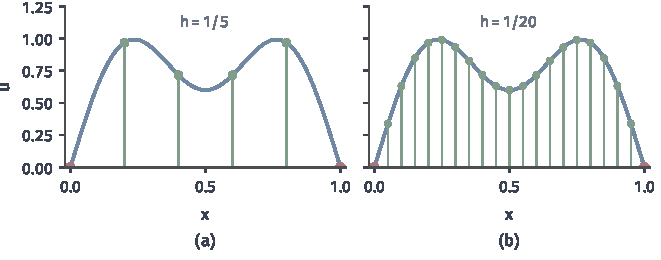
\includegraphics[width=112.0mm]{figures/06-differential-equations/02-partial-differential-equations/matplotlib/pdeprob-state-to-field/figure.pdf}
  \caption{细棒上的温度曲线（蓝）及其格点采样（绿）。曲线为$u=\sin\pi x+0.4\sin3\pi x$，两端值为零（红点）。(a)$h=1/5$，状态是$4$维向量。(b)$h=1/20$，状态是$19$维向量。把步长继续减小，向量就变成整条曲线。}
  \label{fig:pdeprob-state-to-field}
\end{BookInlineFigure}

步长趋于零时，状态不再是有限个数，而是一个函数。这样在空间每一点指定一个量的函数称为\term{场}（field）。每点的量是一个数，就是\term{标量场}（scalar field），如温度、浓度、弦的位移；每点的量是一个向量，就是\term{向量场}（vector field），如流体的速度。

\paragraph{本部分的记号}
从本章开始，空间区域记为开集$\Omega\subset\mathbb{R}^{d}$，边界为$\partial\Omega$，闭包为$\overline{\Omega}$，边界上的单位外法向为$\bm{n}$。空间点写作$\bm{x}$，一维时写作$x$。这里要特别注意：第一部分用$\bm{x}(t)$表示状态，而在这一部分$\bm{x}$只表示位置，状态的角色由整个函数$u(\cdot,t)$担任。

偏导数写作$\partial_tu$、$\partial_xu$、$\partial_{x_i}u$。三个空间微分算子只对$\bm{x}$求导，不涉及$t$，它们是：
\begin{equation}
  \begin{gathered}
    \nabla u=(\partial_{x_1}u,\ldots,\partial_{x_d}u)^{\top},\qquad
    \nabla\cdot\bm{F}=\sum_{i=1}^{d}\partial_{x_i}F_i,\\
    \Delta u=\nabla\cdot(\nabla u)=\sum_{i=1}^{d}\partial_{x_i}^{2}u.
  \end{gathered}
  \label{eq:pdeprob-operators}
\end{equation}
三者分别称为梯度、散度和Laplace算子。这些场运算的定义和计算规则与积分定理配套，可参考\BookChapterRef{chap:integral-theorems}{卷二第27章“积分定理”}。方程中其余各量的写法列在表~\ref{tab:pdeprob-notation}中，后面各章沿用。

\begin{BookInlineTable}
  \centering
  \begin{tabular}{lll}
    \toprule
    记号 & 含义 & 所在位置\\
    \midrule
    $u(\bm{x},t)$ & 未知场 & $\Omega$内 \\
    $f$ & 源项 & $\Omega$内 \\
    $u_0$ & 初值 & $t=0$的$\Omega$上 \\
    $g$ & 边值 & $\partial\Omega$上 \\
    $\bm{A}(\bm{x})$ & 扩散系数矩阵，对称正定 & $\Omega$内 \\
    $\bm{v}(\bm{x},t)$ & 速度场 & $\Omega$内 \\
    $F(u)$ & 依赖于$u$的通量 & 守恒律中 \\
    $H$ & Hamilton量 & Hamilton--Jacobi方程中 \\
    \bottomrule
  \end{tabular}
  \caption{偏微分方程部分的数据记号。}
  \label{tab:pdeprob-notation}
\end{BookInlineTable}

\paragraph{由局部守恒得到方程}
方程的形式并不是约定出来的，它来自物理量的收支。设$u$是某种量的密度，如热量或墨水浓度，$\bm{F}(\bm{x},t)$是通量，表示单位时间穿过单位面积的量，$f$是单位体积内的产生率。任取一块包含在$\Omega$内的小区域$V$，如图~\ref{fig:pdeprob-balance}。$V$内总量的变化率等于流入减去流出，再加上内部产生：
\begin{equation}
  \frac{\mathrm{d}}{\mathrm{d}t}\int_V u\,\mathrm{d}\bm{x}
  =-\int_{\partial V}\bm{F}\cdot\bm{n}\,\mathrm{d}S+\int_V f\,\mathrm{d}\bm{x}.
  \label{eq:pdeprob-balance}
\end{equation}

\begin{BookInlineFigure}
  \centering
  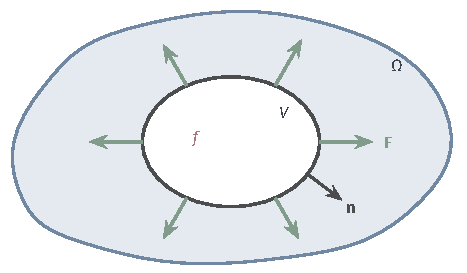
\includegraphics[width=79.1mm]{figures/06-differential-equations/02-partial-differential-equations/tikz/pdeprob-balance/figure.pdf}
  \caption{局部收支。浅蓝区域是$\Omega$，白色小区域$V$内有产生率$f$，绿色箭头表示穿过$\partial V$的通量$\bm{F}$，$\bm{n}$是$\partial V$的单位外法向。$\bm{F}\cdot\bm{n}>0$处量在流出$V$。}
  \label{fig:pdeprob-balance}
\end{BookInlineFigure}

设$u$对$t$连续可微，$\bm{F}$对$\bm{x}$连续可微，$V$的边界足够规则。由散度定理，边界积分可以改写成区域积分，式~\eqref{eq:pdeprob-balance}成为
\[
  \int_V\bigl(\partial_tu+\nabla\cdot\bm{F}-f\bigr)\,\mathrm{d}\bm{x}=0.
\]
这对每个小区域$V$都成立。被积函数连续，若它在某点为正，在该点的一个小球上也为正，取$V$为这个小球就与上式矛盾；为负时同理。所以被积函数处处为零，得到局部形式：
\begin{equation}
  \partial_tu+\nabla\cdot\bm{F}=f.
  \label{eq:pdeprob-conservation}
\end{equation}

式~\eqref{eq:pdeprob-conservation}只有一条关系，却有$u$和$\bm{F}$两个未知对象，还要说明通量怎样由$u$决定。这一步由具体的物理规律给出，不同的规律得到不同的方程。

若热量从高温流向低温，流量正比于温度梯度，就有$\bm{F}=-\bm{A}(\bm{x})\nabla u$，其中对称正定矩阵$\bm{A}$描述材料各方向的导热能力。代入后得到扩散型方程：
\begin{equation}
  \partial_tu-\nabla\cdot\bigl(\bm{A}(\bm{x})\nabla u\bigr)=f.
  \label{eq:pdeprob-diffusion-general}
\end{equation}

若量只是被流体带着走，就有$\bm{F}=\bm{v}u$。由乘积法则，
\[
  \nabla\cdot(\bm{v}u)=\bm{v}\cdot\nabla u+u\,\nabla\cdot\bm{v}.
\]
在不可压缩流动$\nabla\cdot\bm{v}=0$中，第二项消失，方程成为输运形式$\partial_tu+\bm{v}\cdot\nabla u=f$。

若通量是密度自身的函数$F(u)$，例如车流量由车辆密度决定，一维方程就是$\partial_tu+\partial_xF(u)=0$。

弦的振动不是量的收支，而是Newton第二定律。设线密度为$\rho$的弦绷有张力$T$，位移$u(x,t)$和斜率都很小。一小段$[x,x+\delta]$受到两端张力的竖直分力，近似为$T\partial_xu(x+\delta,t)-T\partial_xu(x,t)$，所以
\[
  \rho\,\delta\,\partial_t^{2}u\approx T\bigl(\partial_xu(x+\delta,t)-\partial_xu(x,t)\bigr).
\]
两边除以$\rho\delta$，令$\delta\to0$，并记$c^{2}=T/\rho$，就得到$\partial_t^{2}u=c^{2}\partial_x^{2}u$。

\paragraph{四个模型方程}
取$\bm{A}=\bm{I}$，让演化方程的时间变化率消失，就得到平衡状态的方程。于是我们有四个代表性的方程，它们用同一组变量写成：
\begin{align}
  -\Delta u&=f, \label{eq:pdeprob-poisson}\\
  \partial_tu+\bm{v}\cdot\nabla u&=f, \label{eq:pdeprob-transport}\\
  \partial_tu-\Delta u&=f, \label{eq:pdeprob-heat}\\
  \partial_t^{2}u-c^{2}\Delta u&=f. \label{eq:pdeprob-wave}
\end{align}
依次称为\term{Poisson方程}（Poisson equation）、\term{输运方程}（transport equation）、\term{热方程}（heat equation）和\term{波动方程}（wave equation）。

式~\eqref{eq:pdeprob-poisson}中没有$t$，解只依赖位置，这样的场称为\term{静态场}（stationary field），如稳态温度、膜在固定载荷下的位移。另外三个方程含$t$，解是\term{演化场}（evolving field）。静态问题没有起点，只受区域和边界约束；演化问题的状态从某个时刻出发向前推进，这个差别决定了后面需要什么样的数据。

式~\eqref{eq:pdeprob-heat}和式~\eqref{eq:pdeprob-wave}都含$\Delta u$，要理解这两个方程先要知道$\Delta u$量的是什么。设$u$对$x$三次连续可微，由Taylor展开，
\begin{equation}
  \frac{u(x+h)+u(x-h)}{2}-u(x)=\frac{h^{2}}{2}\partial_x^{2}u(x)+o(h^{2}).
  \label{eq:pdeprob-neighbor-average}
\end{equation}
左边是两个邻点的平均减去当前值。所以$\partial_x^{2}u<0$表示这一点高于邻点的平均，处在凸起上；$\partial_x^{2}u>0$表示这一点低于邻点的平均。

图~\ref{fig:pdeprob-laplace-average}中，红点在峰顶时比两邻点连线的中点高，在山脚时比它低。热方程说温度变化率就是这个差：峰顶降温，山脚升温，形状被抹平。

\begin{BookInlineFigure}
  \centering
  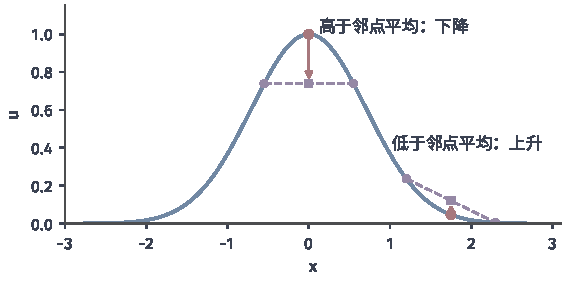
\includegraphics[width=96.0mm]{figures/06-differential-equations/02-partial-differential-equations/matplotlib/pdeprob-laplace-average/figure.pdf}
  \caption{二阶导数比较一点与其邻点的平均。蓝线为$u=\mathrm{e}^{-x^2}$，紫色虚线连接邻点$x_0\pm0.55$，紫色方块是两邻点的平均，红点是$u(x_0)$，红色箭头指示热方程下该点的变化方向。}
  \label{fig:pdeprob-laplace-average}
\end{BookInlineFigure}

在$d$维中，把两个邻点换成以$\bm{x}$为心、半径$r$的球面，同样的Taylor展开给出球面平均减去中心值约等于$\frac{r^{2}}{2d}\Delta u(\bm{x})$。这里用到单位球面上$n_in_j$的平均值，$i=j$时为$1/d$，$i\neq j$时为$0$。$f=0$时这个主项消失；事实上此时两者精确相等，这就是平衡状态下每一点的值等于周围平均的性质。

图~\ref{fig:pdeprob-three-evolutions}把同一个初始鼓包放进三个演化方程。热方程把它压低变宽，输运方程把它原样平移，波动方程把它分成两半向两侧传播。这三种行为分别对应抹平、搬运和分路传播，后面几章会分别加以证明。

\begin{BookInlineFigure}
  \centering
  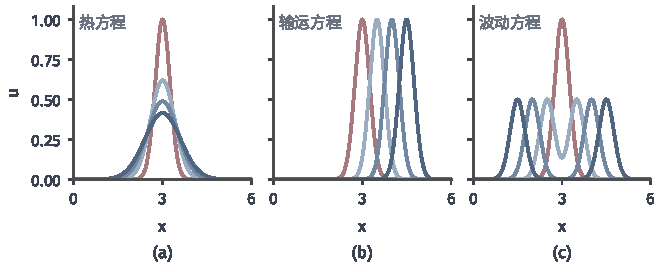
\includegraphics[width=112.0mm]{figures/06-differential-equations/02-partial-differential-equations/matplotlib/pdeprob-three-evolutions/figure.pdf}
  \caption{同一鼓包$u_0(x)=\exp(-(x-3)^2/(2\cdot0.25^2))$在实轴上的演化，红线为$t=0$，蓝色由浅到深为$t=0.5,1,1.5$。(a)$\partial_tu=0.1\,\partial_x^2u$，方差由$0.25^2$增至$0.25^2+0.2t$。(b)$\partial_tu+\partial_xu=0$，解为$u_0(x-t)$。(c)$\partial_t^2u=\partial_x^2u$，初速度为零，解为$\frac12[u_0(x-t)+u_0(x+t)]$。}
  \label{fig:pdeprob-three-evolutions}
\end{BookInlineFigure}

\paragraph{一般形式与线性程度}
上面的方程都是在每一点上把未知函数和它的有限个偏导数联系起来。把静态和演化两种情形放在一起，记自变量为$\bm{z}$：静态问题中$\bm{z}=\bm{x}$，演化问题中$\bm{z}=(\bm{x},t)$。用$D^{k}u$表示$u$的全部$k$阶偏导数。

\begin{definition}[偏微分方程]
\label{def:pdeprob-pde}
设$U$是自变量$\bm{z}$所在的开集，$u:U\to\mathbb{R}$是未知函数。若在$U$的每一点上，$u$及其不超过$m$阶的偏导数满足关系
\begin{equation}
  \mathcal{F}\bigl(\bm{z},u,Du,\ldots,D^{m}u\bigr)=0,
  \label{eq:pdeprob-general-form}
\end{equation}
且$\mathcal{F}$确实依赖某个$m$阶偏导数，则称它是$m$阶\term{偏微分方程}（partial differential equation, PDE）。
\end{definition}

方程按对最高阶导数和$u$的依赖方式分为几个层次，见表~\ref{tab:pdeprob-linearity}。线性方程的系数只依赖$\bm{z}$，算子$L$满足$L(au+bw)=aLu+bLw$；\term{半线性方程}（semilinear equation）的最高阶部分线性，且系数只依赖$\bm{z}$，低阶部分可以非线性；\term{拟线性方程}（quasilinear equation）的最高阶导数仍以一次形式出现，但系数可以依赖$u$和较低阶导数；\term{完全非线性方程}（fully nonlinear equation）对最高阶导数本身非线性。

\begin{BookInlineTable}
  \centering
  \begin{tabular}{lll}
    \toprule
    层次 & 例子 & 判断依据\\
    \midrule
    线性 & $\partial_tu-\nabla\cdot(\bm{A}(\bm{x})\nabla u)=f$ & 系数只依赖$\bm{x}$\\
    半线性 & $\partial_tu-\Delta u=u^{2}$ & 最高阶线性，低阶$u^{2}$\\
    拟线性 & $\partial_tu+u\,\partial_xu=0$ & $\partial_xu$的系数含$u$\\
    完全非线性 & $\partial_tu+\frac12(\partial_xu)^{2}=0$ & 最高阶导数出现平方\\
    \bottomrule
  \end{tabular}
  \caption{偏微分方程按线性程度的层次。}
  \label{tab:pdeprob-linearity}
\end{BookInlineTable}

这些区分影响求解方式。线性方程满足叠加：两个解的线性组合对相应右端仍是解，两个解之差满足右端为零的方程，这是证明唯一性时的基本手段。非线性方程没有这一性质，下面用拟线性方程$\partial_tu+u\,\partial_xu=0$算一个例子。

取两个解$u_1=1$和$u_2=x/(1+t)$。常数$u_1$的两个偏导数都是零，它满足方程。$u_2$的偏导数为
\[
  \partial_tu_2=-\frac{x}{(1+t)^{2}},\qquad
  u_2\,\partial_xu_2=\frac{x}{1+t}\cdot\frac{1}{1+t}=\frac{x}{(1+t)^{2}},
\]
两者相加为零。再看$w=u_1+u_2=1+x/(1+t)$，同样计算得
\[
  \partial_tw+w\,\partial_xw=-\frac{x}{(1+t)^{2}}+\Bigl(1+\frac{x}{1+t}\Bigr)\frac{1}{1+t}=\frac{1}{1+t}\neq0.
\]
两个解之和不是解。

其余几项的作用也可以逐一说清。阶数$m$决定经典意义下解要有几阶导数，也关系到要提供多少数据。系数是常数时，方程在平移下不变，可以用Fourier模式把求导变成乘法；系数随位置变化时这条路不再直接可用。源项$f$让方程非齐次，但在线性问题中可以通过取差消去。

\paragraph{向量未知量}
未知量也可以是向量场。把波动方程降阶就能得到一个例子，做法和常微分方程降阶相同。在一维中记$p=\partial_tu$，$q=\partial_xu$，波动方程$\partial_t^{2}u=c^{2}\partial_x^{2}u$和混合偏导相等分别给出
\[
  \partial_tp=c^{2}\partial_xq,\qquad \partial_tq=\partial_xp.
\]
记$\bm{w}=(p,q)^{\top}$，这是一个一阶方程组：
\begin{equation}
  \partial_t\bm{w}=\bm{B}\,\partial_x\bm{w},\qquad
  \bm{B}=\begin{pmatrix}0&c^{2}\\1&0\end{pmatrix}.
  \label{eq:pdeprob-first-order-system}
\end{equation}
$\bm{B}$的特征值是$\pm c$，恰好是波向两侧传播的速度。降阶用未知量的个数换取了导数的阶数；流体的速度场方程、电磁场方程也是这样的方程组。本部分以标量未知量为主。

\paragraph{函数作为无限维向量}
回到细棒，看空间离散后方程变成什么。在内部格点上用式~\eqref{eq:pdeprob-neighbor-average}近似$\partial_x^{2}u$，并取两端值为零，记$\bm{u}(t)=(u_1(t),\ldots,u_N(t))^{\top}$，热方程成为线性常微分方程组：
\begin{equation}
  \frac{\mathrm{d}\bm{u}}{\mathrm{d}t}=\bm{A}_h\bm{u},\qquad
  (\bm{A}_h\bm{u})_j=\frac{u_{j+1}-2u_j+u_{j-1}}{h^{2}}.
  \label{eq:pdeprob-semi-discrete}
\end{equation}
式中下标超出$1,\ldots,N$的格点值取为零，这样两端的零边值已经写进矩阵。

下面取$N=3$，$h=1/4$，逐项算出这个矩阵的特征值：
\[
  \bm{A}_h=16\begin{pmatrix}-2&1&0\\1&-2&1\\0&1&-2\end{pmatrix}.
\]
$\bm{A}_h$的第$k$个特征向量由$\sin(k\pi x_j)$组成，由和差化积，特征值是
\[
  \lambda_k=-\frac{4}{h^{2}}\sin^{2}\frac{k\pi h}{2},\qquad k=1,\ldots,N.
\]
代入$h=1/4$，得到
\[
  \lambda_1\approx-9.37,\quad \lambda_2=-32,\quad \lambda_3\approx-54.63.
\]

连续问题中对应的等式是
\[
  \partial_x^{2}\sin(k\pi x)=-k^{2}\pi^{2}\sin(k\pi x),
\]
前三个特征值约为$-9.87$、$-39.48$、$-88.83$。向量的分量对应函数在各点的值，矩阵$\bm{A}_h$对应算子$\partial_x^{2}$，特征向量对应正弦模式，矩阵的首末行编码了零边值。

这个类比在一个关键处失效。图~\ref{fig:pdeprob-spectrum-growth}显示，低频特征值随加密趋于$-k^{2}\pi^{2}$，但矩阵的谱范数约为$4/h^{2}$，$N\to\infty$时趋于无穷。

\begin{BookInlineFigure}
  \centering
  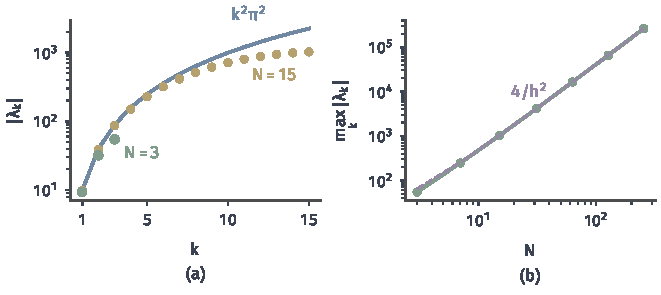
\includegraphics[width=112.0mm]{figures/06-differential-equations/02-partial-differential-equations/matplotlib/pdeprob-spectrum-growth/figure.pdf}
  \caption{式~\eqref{eq:pdeprob-semi-discrete}中矩阵的特征值。(a)第$k$个特征值的绝对值：$N=3$（绿）、$N=15$（黄）、连续问题的$k^2\pi^2$（蓝）。(b)最大特征值绝对值（绿）随$N$的增长，紫色虚线为$4/h^2$。}
  \label{fig:pdeprob-spectrum-growth}
\end{BookInlineFigure}

谱范数正是线性右端的Lipschitz常数。第~\ref{chap:ode-existence-continuation}章的存在性论证依赖右端的Lipschitz条件，而这里的常数随加密无界增长，极限算子$\partial_x^{2}$在$L^{2}(0,1)$或$C[0,1]$这样的空间上不是有界映射：它要消耗两阶导数。所以不能把偏微分方程直接当作无限维常微分方程来套用已有的定理。后面要靠别的结构，例如$\bm{A}_h$的特征值全部为负，来得到估计；这也是为什么必须先说清解和数据所在的空间。

\section{初值与边界数据}
\label{sec:pdeprob-data}

方程只规定区域内部每一点上的局部关系，它本身确定不了解。仍以$(0,1)$上的细棒为例，下面几个函数都满足$\partial_tu=\partial_x^{2}u$：
\[
  u=0,\qquad u=x,\qquad u=x^{2}+2t,\qquad u=\mathrm{e}^{-\pi^{2}t}\sin\pi x.
\]
第三个函数的两个偏导数都是$2$；第四个函数的两个偏导数都等于$-\pi^{2}\mathrm{e}^{-\pi^{2}t}\sin\pi x$。

缺少的信息有多少？一阶常微分方程的通解含一个任意常数，补一个初值就够了。偏微分方程的通解含任意函数。例如$\partial_tu+\partial_xu=0$的解可以写成$u=\varphi(x-t)$，其中$\varphi$是任意可微函数，由链式法则，$\partial_tu=-\varphi'$，$\partial_xu=\varphi'$，两者相加为零。所以需要补充的也是函数，它们定义在比时空低一维的集合上：初始时刻的切片和区域的边界。

演化问题的自变量落在\term{时空柱}（space-time cylinder）$Q=\Omega\times(0,T)$中。图~\ref{fig:pdeprob-cylinder}画出它的三块边界：底面是初始时刻，侧面是空间边界随时间展开，顶面是终止时刻。以热方程为例，典型的问题是
\begin{equation}
  \begin{cases}
    \partial_tu-\Delta u=f & \text{在}\ Q\ \text{内},\\
    u=g & \text{在}\ \partial\Omega\times(0,T)\ \text{上},\\
    u(\cdot,0)=u_0 & \text{在}\ \Omega\ \text{上}.
  \end{cases}
  \label{eq:pdeprob-heat-ibvp}
\end{equation}

\begin{BookInlineFigure}
  \centering
  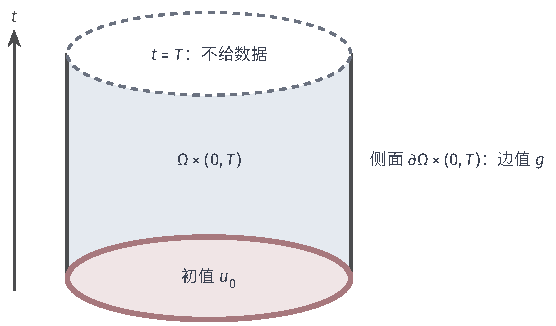
\includegraphics[width=94.1mm]{figures/06-differential-equations/02-partial-differential-equations/tikz/pdeprob-cylinder/figure.pdf}
  \caption{时空柱$Q=\Omega\times(0,T)$。红色底面给初值，深灰色侧面给边值，虚线所示的顶面$t=T$不给数据，那里的值由演化决定。}
  \label{fig:pdeprob-cylinder}
\end{BookInlineFigure}

数据的个数和位置不是随意的，还要与方程传播信息的方式相合。热方程不在顶面给数据，输运方程只在一部分侧面给数据，波动方程在底面要给两个函数。下面分三部分讨论：初始状态要给几个函数、边界上能给什么、两者交接时要满足什么。

\subsection{初始数据}
\label{sec:pdeprob-initial}

为什么热方程只要一个初值，而波动方程要两个？比较这两个方程在$t=0$能告诉我们什么。

\paragraph{时间阶数与初始状态}
在$(0,1)$上给定初始温度$u_0$，且两端为零。热方程的右端可以由$u_0$算出，于是$\partial_tu(\cdot,0)=\partial_x^{2}u_0$，时间一阶导数已经由方程确定，不必再给。

波动方程不同。给定初始位移$u_0$，方程只确定了$\partial_t^{2}u(\cdot,0)=c^{2}\partial_x^{2}u_0$，时间一阶导数还是自由的。这和常微分方程$\ddot{x}=-x$必须同时给位置和速度是一回事，只是位置和速度现在都是函数。所以波动方程的初始状态是一对函数：
\begin{equation}
  u(\cdot,0)=u_0,\qquad \partial_tu(\cdot,0)=u_1.
  \label{eq:pdeprob-wave-initial}
\end{equation}

下面取$c=1$、两端固定，给定同一个初始位移$u_0=\sin\pi x$，算两个不同的解。直接代入可以验证，下面两个函数都满足波动方程和零边值，且在$t=0$的位移都是$\sin\pi x$：
\[
  u^{\mathrm{a}}=\cos(\pi t)\sin\pi x,\qquad
  u^{\mathrm{b}}=\bigl(\cos(\pi t)+\sin(\pi t)\bigr)\sin\pi x.
\]
区别在初始速度：$\partial_tu^{\mathrm{a}}(x,0)=0$，而$\partial_tu^{\mathrm{b}}(x,0)=\pi\sin\pi x$。

图~\ref{fig:pdeprob-wave-velocity}(b)比较弦中点的历史。两条波动曲线从同一点出发，随后分开，所以只给位移不能确定解。同样的初值在热方程下只有一条曲线，就是$\mathrm{e}^{-\pi^{2}t}$，第~\ref{sec:pdeprob-well-posedness}节将证明它是唯一的。

\begin{BookInlineFigure}
  \centering
  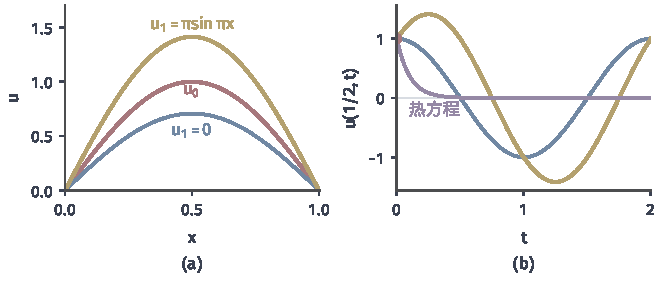
\includegraphics[width=112.0mm]{figures/06-differential-equations/02-partial-differential-equations/matplotlib/pdeprob-wave-velocity/figure.pdf}
  \caption{同一初始位移$u_0=\sin\pi x$（红），$c=1$。(a)$t=1/4$时的弦形：初速度为零（蓝）和初速度为$\pi\sin\pi x$（黄）。(b)中点$x=1/2$的时间历史，蓝、黄同(a)，紫线是热方程在同一初值下的解。}
  \label{fig:pdeprob-wave-velocity}
\end{BookInlineFigure}

一般地，若方程能解出最高阶时间导数，即$\partial_t^{k}u$可以用较低阶时间导数和空间导数表示，就需要$k$个初始函数。这时可以逐阶求出$t=0$处的全部时间导数。以波动方程的$u^{\mathrm{b}}$为例，由初始数据得$\partial_t^{2}u=-\pi^{2}\sin\pi x$，对方程再求一次时间导数得$\partial_t^{3}u=-\pi^{3}\sin\pi x$，这正是$u^{\mathrm{b}}$的Taylor系数。

这个计数只是必要的预期，不保证问题可解。第~\ref{sec:pdeprob-well-posedness}节会看到，把Laplace方程中的一个空间变量当成“时间”，也可以解出二阶导数并给两个初始函数，结果却完全不可用。

\paragraph{初值的光滑程度}
初值的光滑程度决定方程在初始时刻能否按经典意义解释。取折线初值
\begin{equation}
  u_0(x)=\min\{x,1-x\},
  \label{eq:pdeprob-hat}
\end{equation}
它在$x=1/2$处没有导数，$\partial_x^{2}u_0$不存在，所以方程在$t=0$的这一点上没有意义。解决办法是只要求方程在$t>0$成立，初值作为$t\to0$时的极限取到。

这样解释后，热方程和波动方程的表现完全不同。把$u_0$展开成正弦级数，系数为
\[
  b_k=2\int_0^{1}u_0(x)\sin(k\pi x)\,\mathrm{d}x=\frac{4\sin(k\pi/2)}{k^{2}\pi^{2}},
\]
热方程的解和$c=1$的波动方程在初速度为零时的解分别是
\[
  \sum_{k\geq1}b_k\mathrm{e}^{-k^{2}\pi^{2}t}\sin k\pi x,\qquad
  \sum_{k\geq1}b_k\cos(k\pi t)\sin k\pi x.
\]

对热方程，每求一次$x$的导数系数多一个因子$k\pi$，但只要$t>0$，因子$\mathrm{e}^{-k^{2}\pi^{2}t}$比任何多项式衰减得都快，求导后的级数仍然收敛，解立即变得光滑。在$t=0$，二阶导数的级数通项是$-4\sin(k\pi/2)\sin(k\pi x)$，不趋于零，这正对应$\partial_x^{2}u_0$不存在。

对波动方程，系数没有衰减因子。解等于$\frac12[u_0^{*}(x-t)+u_0^{*}(x+t)]$，其中$u_0^{*}$是$u_0$在实轴上的奇周期延拓。折角被原样带着走，分成两个折角向两边移动。图~\ref{fig:pdeprob-kink-heat-wave}对比了两种情形：(a)的折角瞬间变圆，(b)的折角一直保持。所以波动方程在$t>0$时沿这两条线仍不能按经典意义解释；这样的函数算不算解，要到第~\ref{sec:pdeprob-solutions}节再回答。

\begin{BookInlineFigure}
  \centering
  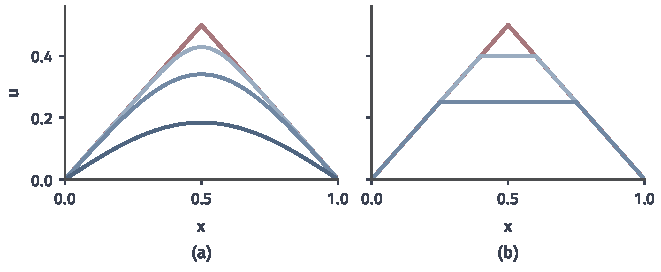
\includegraphics[width=112.0mm]{figures/06-differential-equations/02-partial-differential-equations/matplotlib/pdeprob-kink-heat-wave/figure.pdf}
  \caption{折线初值$u_0=\min\{x,1-x\}$（红），两端为零。(a)热方程，蓝色由浅到深为$t=0.004,0.02,0.08$，折角立即消失（$600$项正弦级数）。(b)波动方程，$c=1$，初速度为零，蓝色由浅到深为$t=0.1,0.25$，两个折角分别向左右移动，中间是一段平台。}
  \label{fig:pdeprob-kink-heat-wave}
\end{BookInlineFigure}

\subsection{边界数据}
\label{sec:pdeprob-boundary}

区域有边界，边界上发生的事也要交代。边界条件规定的可以是场值，可以是穿过边界的通量，也可以是两者之间的关系。

\paragraph{三类边界条件}
记$\partial_{\bm{n}}u=\nabla u\cdot\bm{n}$，它是$u$沿离开区域方向的变化率，称为\term{法向导数}（normal derivative）。按照热传导的语言，$\partial\Omega$上常见的条件是：
\begin{align}
  u&=g, \label{eq:pdeprob-dirichlet}\\
  \partial_{\bm{n}}u&=g, \label{eq:pdeprob-neumann}\\
  \partial_{\bm{n}}u+\alpha u&=g. \label{eq:pdeprob-robin}
\end{align}
依次称为\term{Dirichlet边界条件}（Dirichlet boundary condition）、\term{Neumann边界条件}（Neumann boundary condition）和\term{Robin边界条件}（Robin boundary condition）。

Dirichlet条件直接规定温度，如棒端浸在恒温水中。Neumann条件规定穿过边界的通量，向外的热流是$-\partial_{\bm{n}}u$，所以$g=0$表示绝热。Robin条件来自Newton冷却定律：向外的热流正比于边界温度与环境温度$u_{\mathrm{env}}$之差，$-\partial_{\bm{n}}u=\alpha(u-u_{\mathrm{env}})$，整理后就是式~\eqref{eq:pdeprob-robin}，其中$g=\alpha u_{\mathrm{env}}$。

物理上$\alpha\geq0$。$\alpha<0$意味着边界越热吸收得越多，这种正反馈下后面的估计不再成立。系数不是单位矩阵时，通量是$\bm{A}\nabla u$，法向导数相应换成$\bm{n}^{\top}\bm{A}\nabla u$。不同边界段可以使用不同类型，如图~\ref{fig:pdeprob-boundary-types}。

\begin{BookInlineFigure}
  \centering
  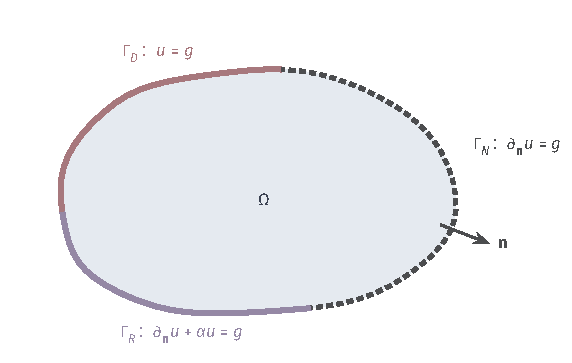
\includegraphics[width=96.9mm]{figures/06-differential-equations/02-partial-differential-equations/tikz/pdeprob-boundary-types/figure.pdf}
  \caption{同一区域的边界分成三段：红色段$\Gamma_D$规定场值，深灰虚线段$\Gamma_N$规定法向导数，紫色段$\Gamma_R$规定场值和法向导数的组合。$\bm{n}$是单位外法向。}
  \label{fig:pdeprob-boundary-types}
\end{BookInlineFigure}

边界类型会改变解本身。下面在$(0,1)$上取方程$-u''=2$和右端条件$u(1)=0$，通解是
\[
  u(x)=-x^{2}+Ax+B.
\]
左端点的外法向指向$-x$方向，所以左端的$\partial_{\bm{n}}u=-u'(0)$。下面依次取三种条件。

Dirichlet条件$u(0)=0$给出$B=0$，再由$u(1)=0$得$A=1$，于是
\[
  u(x)=x(1-x),\qquad \max_xu=\frac14.
\]

Neumann条件$u'(0)=0$给出$A=0$，再由$u(1)=0$得$B=1$，于是
\[
  u(x)=1-x^{2},\qquad \max_xu=1.
\]

Robin条件取$\alpha=1$、$g=0$，即$-u'(0)+u(0)=0$，给出$A=B$。再由$u(1)=-1+2B=0$得$B=1/2$，于是
\[
  u(x)=\frac12+\frac12x-x^{2},\qquad \max_xu=u\Bigl(\frac14\Bigr)=\frac{9}{16}.
\]

图~\ref{fig:pdeprob-bc-solutions}中，三条曲线的热源和右端相同，只有左端不同：Dirichlet曲线被钉在零，Neumann曲线的切线水平，Robin曲线的切线斜率等于端点值$1/2$。左端越容易散热，整根棒越凉：Dirichlet、Robin、Neumann三种情形的最高温依次是$1/4$、$9/16$、$1$。

\begin{BookInlineFigure}
  \centering
  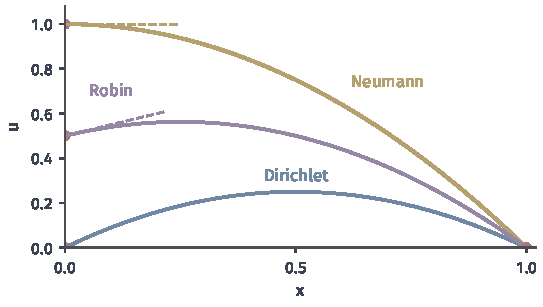
\includegraphics[width=92.0mm]{figures/06-differential-equations/02-partial-differential-equations/matplotlib/pdeprob-bc-solutions/figure.pdf}
  \caption{$-u''=2$、$u(1)=0$在三种左端条件下的解。红点是端点值，虚线是左端切线。}
  \label{fig:pdeprob-bc-solutions}
\end{BookInlineFigure}

\paragraph{输运方程的入流边界}
对$\Omega$的整个边界都规定数据，在二阶椭圆方程中是合理的，在输运方程中却不行。想象水流搬运墨水：墨水的浓度由上游决定，下游端点流出的是已经确定的东西，不能再规定。

在$(0,1)$上取$v=1$，方程$\partial_tu+\partial_xu=0$的信息沿直线$x=x_0+t$传递。设$u(\cdot,0)=u_0$，左端$u(0,t)=g(t)$，沿着这些路径回溯，解是
\begin{equation}
  u(x,t)=\begin{cases}u_0(x-t),&x>t,\\ g(t-x),&x<t.\end{cases}
  \label{eq:pdeprob-transport-solution}
\end{equation}
右端的值$u(1,t)$已经由式~\eqref{eq:pdeprob-transport-solution}确定。若再独立规定$u(1,t)=h(t)$，除非$h$恰好等于算出来的值，否则问题无解。

一般地，定义\term{入流边界}（inflow boundary）和\term{出流边界}（outflow boundary）为
\begin{equation}
  \Gamma_{-}=\{\bm{x}\in\partial\Omega:\bm{v}\cdot\bm{n}<0\},\qquad
  \Gamma_{+}=\{\bm{x}\in\partial\Omega:\bm{v}\cdot\bm{n}>0\}.
  \label{eq:pdeprob-inflow}
\end{equation}
$\bm{v}\cdot\bm{n}<0$表示流动指向区域内部，边界数据只在$\Gamma_{-}$上给出；$\bm{v}$随时间变化时，这两部分也随时间变化。入流边界的位置由速度场决定，而不是由几何形状决定。

图~\ref{fig:pdeprob-inflow}画出区间上的三个速度场。(a)$v=1$，只有左端入流。(b)$v=x-1/2$，两端的外法向分别与速度同向，都是出流，因此端点不需要任何数据，解完全由初值决定。(c)$v=1/2-x$，两端都是入流，都要给数据。

\begin{BookInlineFigure}
  \centering
  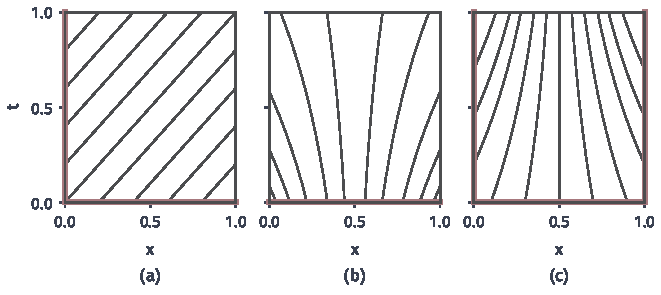
\includegraphics[width=112.0mm]{figures/06-differential-equations/02-partial-differential-equations/matplotlib/pdeprob-inflow/figure.pdf}
  \caption{区间$(0,1)$上三个速度场的粒子路径$\mathrm{d}x/\mathrm{d}t=v$（深灰），红色粗线是需要给数据的边界。(a)$v=1$。(b)$v=x-\frac12$，两端都是出流。(c)$v=\frac12-x$，两端都是入流。每条路径都从红线出发。}
  \label{fig:pdeprob-inflow}
\end{BookInlineFigure}

只在入流边界给数据为什么足够？设$\nabla\cdot\bm{v}=0$，$u$是光滑解，$f=0$。将方程乘以$u$并在$\Omega$上积分。由$\nabla\cdot\bm{v}=0$，对流项可以写成散度：
\[
  u\,\bm{v}\cdot\nabla u=\frac12\nabla\cdot(\bm{v}u^{2}).
\]
再由散度定理，得到
\begin{equation}
  \frac{\mathrm{d}}{\mathrm{d}t}\frac12\int_\Omega u^{2}\,\mathrm{d}\bm{x}
  =-\frac12\int_{\partial\Omega}(\bm{v}\cdot\bm{n})\,u^{2}\,\mathrm{d}S.
  \label{eq:pdeprob-transport-energy}
\end{equation}
出流边界上$\bm{v}\cdot\bm{n}>0$，这一项只会减少能量，不需要控制；入流边界上这一项会增加能量，必须由数据控制。若两个解的初值相同、入流数据相同，它们之差$w$满足式~\eqref{eq:pdeprob-transport-energy}，且$\Gamma_{-}$上$w=0$，所以$\int_\Omega w^{2}$不增，从零出发恒为零。入流数据恰好足以确定解。

\subsection{数据相容性}
\label{sec:pdeprob-compatibility}

初值和边值是分别给出的，但它们在角点处相遇；有些问题的数据之间还有整体的约束。给的数据多，并不意味着有解。

\paragraph{角点处的相容条件}
回到$(0,1)$上的细棒。若初始温度处处为$1$，两端却保持为$0$，那么在角点$(x,t)=(0,0)$附近，沿$t=0$趋近得到$1$，沿$x=0$趋近得到$0$，解不可能在角点连续。

要让解在$\overline{Q}$上连续，需要初值在边界上的取值和边值在初始时刻一致，即零阶\term{相容条件}（compatibility condition）：
\begin{equation}
  u_0(\bm{x})=g(\bm{x},0),\qquad \bm{x}\in\partial\Omega.
  \label{eq:pdeprob-compat-zero}
\end{equation}

要求解更光滑时条件也更多。假设$u$在角点附近有连续的$\partial_tu$和$\partial_x^{2}u$，在左端$x=0$上有$u(0,t)=g(t)$，对$t$求导得$\partial_tu(0,t)=g'(t)$。令$t\to0$，再利用热方程$\partial_tu=\partial_x^{2}u+f$，就得到一阶相容条件：
\begin{equation}
  g'(0)=u_0''(0)+f(0,0).
  \label{eq:pdeprob-compat-one}
\end{equation}
式~\eqref{eq:pdeprob-compat-one}不是额外的物理假设，只是方程在角点处的推论。若要求解有更高阶的连续导数，同样的步骤可以继续，每多要求一阶时间导数，就多一个条件。波动方程的情形类似，表~\ref{tab:pdeprob-compatibility}列出左端点的前几个条件，其中$g$是左端的边值。

\begin{BookInlineTable}
  \centering
  \begin{tabular}{lll}
    \toprule
    方程 & 希望连续到角点的量 & 相容条件\\
    \midrule
    热方程 & $u$ & $u_0(0)=g(0)$\\
    热方程 & $u,\partial_tu,\partial_x^{2}u$ & 另加$g'(0)=u_0''(0)+f(0,0)$\\
    波动方程 & $u$ & $u_0(0)=g(0)$\\
    波动方程 & $u,\partial_tu$ & 另加$u_1(0)=g'(0)$\\
    波动方程 & 全部二阶导数 & 另加$g''(0)=c^{2}u_0''(0)+f(0,0)$\\
    \bottomrule
  \end{tabular}
  \caption{角点处的相容条件随所要求的光滑程度增加。}
  \label{tab:pdeprob-compatibility}
\end{BookInlineTable}

相容条件不满足时，问题不一定无解，而是解的光滑性受限，受限的方式随方程而不同。图~\ref{fig:pdeprob-corner-mismatch}比较初值为$1$、边值为$0$时的两种情形。(a)热方程的解在$t>0$时光滑，不连续性只局限在角点。(b)输运方程的解由式~\eqref{eq:pdeprob-transport-solution}给出，在直线$x=t$左侧为$0$、右侧为$1$，角点处的矛盾被带进区域内部，变成一条持续的间断线。

\begin{BookInlineFigure}
  \centering
  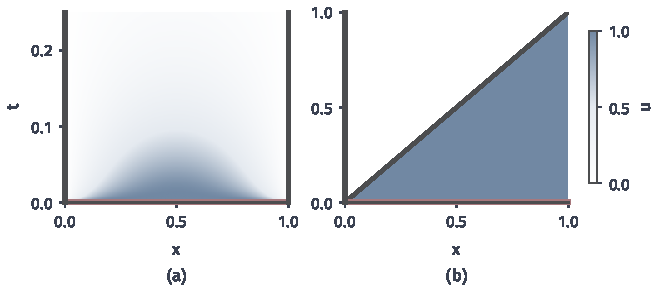
\includegraphics[width=112.0mm]{figures/06-differential-equations/02-partial-differential-equations/matplotlib/pdeprob-corner-mismatch/figure.pdf}
  \caption{初值$u_0=1$（红线）与边值$0$（深灰竖线）不相容。颜色表示$u$的值。(a)热方程，由奇数项正弦级数$\sum_{k}\frac{4}{k\pi}\mathrm{e}^{-k^2\pi^2t}\sin k\pi x$计算。(b)输运方程$v=1$，深灰斜线是间断线$x=t$。两图的时间范围不同。}
  \label{fig:pdeprob-corner-mismatch}
\end{BookInlineFigure}

\paragraph{整体的积分约束}
相容不只发生在角点。考虑Poisson方程配Neumann条件：
\begin{equation}
  -\Delta u=f\ \ \text{在}\ \Omega\ \text{内},\qquad
  \partial_{\bm{n}}u=g\ \ \text{在}\ \partial\Omega\ \text{上},
  \label{eq:pdeprob-neumann-problem}
\end{equation}
其中$\Omega$有界，边界足够规则。把方程在$\Omega$上积分，由散度定理，
\[
  \int_\Omega\Delta u\,\mathrm{d}\bm{x}=\int_{\partial\Omega}\partial_{\bm{n}}u\,\mathrm{d}S.
\]
于是若解存在，数据必须满足
\begin{equation}
  \int_\Omega f\,\mathrm{d}\bm{x}+\int_{\partial\Omega}g\,\mathrm{d}S=0.
  \label{eq:pdeprob-neumann-compat}
\end{equation}

这个条件的含义是收支平衡。$\int f$是内部的总产热，$\int g=\int\partial_{\bm{n}}u$是从外部流入的总热量，平衡状态要求两者之和为零。一个绝热的棒内部持续加热，不可能达到稳态。

在$(0,1)$上取$f=1$、两端绝热$u'(0)=u'(1)=0$。式~\eqref{eq:pdeprob-neumann-compat}左边是$1\neq0$，方程$-u''=1$无解。对应的演化问题$\partial_tu=\partial_x^{2}u+1$却有解，例如从$u_0=\frac12\cos\pi x$出发，
\[
  u(x,t)=t+\frac12\mathrm{e}^{-\pi^{2}t}\cos\pi x.
\]
图~\ref{fig:pdeprob-neumann-balance}(a)中，形状的起伏很快消失，而整体温度以速度$1$不断上升，没有稳态可趋近。

现在改为边界散热，取$u'(0)=1/2$，$u'(1)=-1/2$。这时$\partial_{\bm{n}}u$在两端都是$-1/2$，式~\eqref{eq:pdeprob-neumann-compat}左边是$1-\frac12-\frac12=0$。逐次积分得到解
\[
  u(x)=-\frac{x^{2}}{2}+\frac{x}{2}+C,
\]
其中$C$是任意常数，如图~\ref{fig:pdeprob-neumann-balance}(b)。约束满足了，解却不唯一：方程和边界条件都只含$u$的导数，看不到整体平移。

\begin{BookInlineFigure}
  \centering
  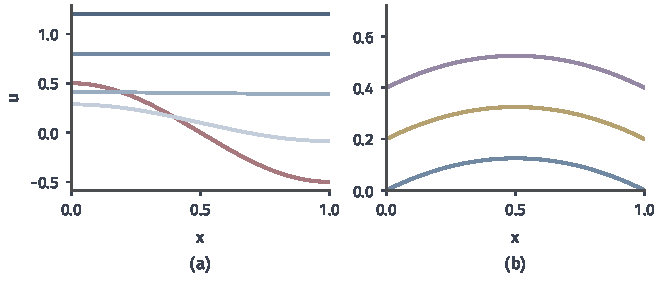
\includegraphics[width=112.0mm]{figures/06-differential-equations/02-partial-differential-equations/matplotlib/pdeprob-neumann-balance/figure.pdf}
  \caption{Neumann问题的积分约束。(a)绝热棒内持续加热，初值（红）的起伏消失，整体上升，蓝色由浅到深为$t=0.1,0.4,0.8,1.2$。(b)加热与散热平衡时$-u''=1$的解$-x^2/2+x/2+C$，$C=0,0.2,0.4$，彼此只差常数。}
  \label{fig:pdeprob-neumann-balance}
\end{BookInlineFigure}

这和线性方程组完全相同。把棒分成三段，每段写热量收支，绝热端没有通量，得到系数矩阵
\[
  \bm{B}=\begin{pmatrix}1&-1&0\\-1&2&-1\\0&-1&1\end{pmatrix},
  \qquad \bm{B}\bm{1}=\bm{0},\qquad \bm{1}^{\top}\bm{B}=\bm{0}^{\top},
\]
其中$\bm{1}=(1,1,1)^{\top}$。方程$\bm{B}\bm{u}=\bm{b}$有解当且仅当$\bm{1}^{\top}\bm{b}=0$，有解时解差$\bm{1}$的倍数。积分约束对应对$\bm{1}$的正交条件，任意常数对应零空间。

这些例子说明，不能靠增加数据的数量来保证有解。数据太少时解不唯一，例如区间上$-u''=f$只给一个端点；数据太多时互相冲突，例如输运方程同时规定两端；个数恰好，也可能违反积分约束。判断的依据是方程的传播方式和结构，下一节把这件事说清楚。

\section{方程类型}
\label{sec:pdeprob-types}

Poisson方程、热方程和波动方程都是二阶线性方程，需要的数据却不同，传播信息的方式也不同。能否不解方程，只看系数就把它们区分开？

\paragraph{主部与高频响应}
记自变量为$\bm{z}\in\mathbb{R}^{N}$，二阶线性方程写成
\begin{equation}
  \sum_{i,j=1}^{N}M_{i,j}(\bm{z})\,\partial_{z_i}\partial_{z_j}u+(\text{一阶及零阶项})=f,
  \label{eq:pdeprob-second-order}
\end{equation}
其中$\bm{M}(\bm{z})$是实对称矩阵。对称性不是限制：混合偏导相等，$M_{i,j}$与$M_{j,i}$只有两者之和起作用，可以都换成平均值。二阶项的全体称为方程的\term{主部}（principal part）。

为什么分类只看主部？在一点附近把系数看成常数，代入高频振荡$u=\mathrm{e}^{\mathrm{i}\bm{\xi}\cdot\bm{z}}$。二阶项给出因子$-\bm{\xi}^{\top}\bm{M}\bm{\xi}$，大小与$\lVert\bm{\xi}\rVert_2^{2}$同阶，一阶项只有$\lVert\bm{\xi}\rVert_2$的量级。频率越高，主部越占支配地位。

所以方程对高频振荡的反应由二次型$\bm{\xi}^{\top}\bm{M}\bm{\xi}$决定。若对所有非零$\bm{\xi}$它都不为零，任何方向的高频振荡都会被主部放大成很大的量，无法存在于解中，除非右端也这样振荡；若沿某个方向它等于零，主部感觉不到沿这个方向的振荡，这种振荡就可以在解中传播。二次型的性质由$\bm{M}$的特征值的符号决定。

\begin{definition}[二阶线性方程的类型]
\label{def:pdeprob-types}
设$\bm{M}(\bm{z})$是式~\eqref{eq:pdeprob-second-order}在点$\bm{z}$处的系数矩阵。根据它的特征值，称方程在该点是
\begin{enumerate}
  \item \term{椭圆型}（elliptic）：全部特征值非零且同号；
  \item \term{抛物型}（parabolic）：恰有一个特征值为零，其余同号，且相应零特征方向上有一阶项；
  \item \term{双曲型}（hyperbolic）：全部特征值非零，且恰有一个的符号与其余相反。
\end{enumerate}
\end{definition}

这三类并不穷尽所有情形。$N\geq4$时可以有两正两负的特征值，例如下面的方程不属于这三类：
\[
  \partial_{z_1}^{2}u+\partial_{z_2}^{2}u-\partial_{z_3}^{2}u-\partial_{z_4}^{2}u=0.
\]

抛物型的定义中要求一阶项，是因为把$\partial_x^{2}u=0$看成$(x,t)$的方程时，$\bm{M}$也有零特征值，但其中$t$只是参数，方程实质上是关于$x$的常微分方程。

把四个模型代入。Poisson方程的$\bm{z}=\bm{x}$，$\bm{M}=-\bm{I}$，椭圆型。热方程的$\bm{z}=(\bm{x},t)$，
\[
  \bm{M}=\operatorname{diag}(-1,\ldots,-1,0),
\]
零特征方向是时间方向，那里有一阶项$\partial_tu$，抛物型。波动方程的$\bm{z}=(\bm{x},t)$，
\[
  \bm{M}=\operatorname{diag}(-c^{2},\ldots,-c^{2},1),
\]
恰有一个特征值与其余反号，双曲型。输运方程是一阶方程，没有二阶项，不在这个分类中。

两个变量时分类有一个常用的判别式。考虑方程
\[
  a_1\partial_y^{2}u+2a_2\partial_y\partial_zu+a_3\partial_z^{2}u+(\text{低阶项})=f.
\]
它的系数矩阵的行列式是$a_1a_3-a_2^{2}$，也就是两个特征值之积。于是$a_2^{2}-a_1a_3$小于零、等于零、大于零分别对应椭圆、抛物、双曲型（抛物型另需一阶项）。

名称来自把$\partial_x$换成$\xi$、把$\partial_t$换成$\tau$后得到的曲线，如图~\ref{fig:pdeprob-conics}：二维Laplace算子给出$\xi^{2}+\tau^{2}=1$，热算子给出$\tau=\xi^{2}$，波动算子给出$\tau^{2}-\xi^{2}=1$。这只解释了名字的来历，真正起作用的是下面要讲的传播方式。

\begin{BookInlineFigure}
  \centering
  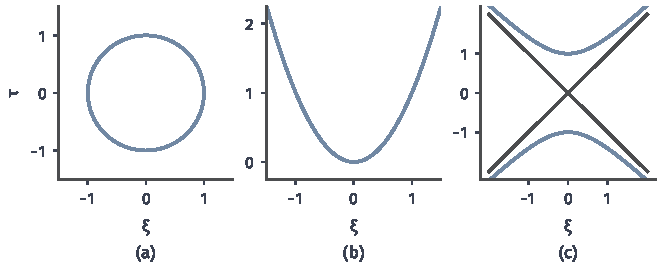
\includegraphics[width=112.0mm]{figures/06-differential-equations/02-partial-differential-equations/matplotlib/pdeprob-conics/figure.pdf}
  \caption{三类方程名称的来历。(a)椭圆$\xi^2+\tau^2=1$。(b)抛物线$\tau=\xi^2$。(c)双曲线$\tau^2-\xi^2=1$，深灰直线是渐近线$\tau=\pm\xi$，它们对应二次型为零的方向。}
  \label{fig:pdeprob-conics}
\end{BookInlineFigure}

\paragraph{分类不依赖坐标}
类型只有在换坐标后不变才有意义。下面的引理说明它只依赖特征值符号的个数。

\begin{lemma}[类型在坐标变换下不变]
\label{lem:pdeprob-invariance}
设$\bm{y}=\bm{\Phi}(\bm{z})$是二阶连续可微的可逆坐标变换，其Jacobi矩阵$\bm{J}$处处可逆。在新坐标下，式~\eqref{eq:pdeprob-second-order}的系数矩阵是
\begin{equation}
  \widetilde{\bm{M}}=\bm{J}\bm{M}\bm{J}^{\top},
  \label{eq:pdeprob-congruence}
\end{equation}
且$\widetilde{\bm{M}}$与$\bm{M}$的正、负、零特征值个数分别相同。
\end{lemma}

\begin{proof}
记$\widetilde{u}(\bm{y})=u(\bm{z})$。由链式法则，
\[
  \partial_{z_i}u=\sum_{k}J_{k,i}\,\partial_{y_k}\widetilde{u}.
\]
再求一次导数，二阶导数项来自对$\partial_{y_k}\widetilde{u}$求导，对$J_{k,i}$求导只产生一阶项，于是
\[
  \partial_{z_i}\partial_{z_j}u=\sum_{k,l}J_{k,i}J_{l,j}\,\partial_{y_k}\partial_{y_l}\widetilde{u}+(\text{一阶项}).
\]
代入式~\eqref{eq:pdeprob-second-order}，$\partial_{y_k}\partial_{y_l}\widetilde{u}$的系数是$\sum_{i,j}J_{k,i}M_{i,j}J_{l,j}$，这就是式~\eqref{eq:pdeprob-congruence}。

$\bm{M}$的正特征值个数等于使二次型在其上正定的子空间的最大维数。变量替换$\bm{\xi}=\bm{J}^{\top}\bm{\eta}$是线性双射，把$\bm{M}$的这类子空间一一映成$\widetilde{\bm{M}}$的这类子空间，维数不变。负特征值同理，零特征值的个数由总数$N$确定。
\end{proof}

\paragraph{特征方向}
引理还回答了哪些曲面特殊。设曲面由$\varphi(\bm{z})=$常数给出，$\nabla_{\bm{z}}\varphi\neq\bm{0}$。若把$\varphi$取作新坐标$y_1$，$\bm{J}$的第一行就是$(\nabla_{\bm{z}}\varphi)^{\top}$，由式~\eqref{eq:pdeprob-congruence}，
\[
  \widetilde{M}_{1,1}=(\nabla_{\bm{z}}\varphi)^{\top}\bm{M}\,\nabla_{\bm{z}}\varphi.
\]
若这个量为零，新方程中不含$\partial_{y_1}^{2}\widetilde{u}$，方程就无法用曲面上的值和一阶法向导数算出二阶法向导数。这样的曲面称为\term{特征曲面}（characteristic surface），两个自变量时称为\term{特征线}（characteristic curve）。二阶法向导数穿过它可以有跳跃，解的不光滑性可以沿它存在。

下面用一个可以手算的方程走一遍。考虑
\[
  \partial_y^{2}u+4\partial_y\partial_zu+3\partial_z^{2}u=0.
\]
这里$a_1=1$，$a_2=2$，$a_3=3$，判别式$a_2^{2}-a_1a_3=1>0$，方程是双曲型。系数矩阵的两个特征值是$2\pm\sqrt{5}$，确实异号。

把算子分解为两个一阶因子，
\[
  \partial_y^{2}+4\partial_y\partial_z+3\partial_z^{2}=(\partial_y+\partial_z)(\partial_y+3\partial_z).
\]
第一个因子把任何$\psi(y-z)$变成零，第二个因子把任何$\varphi(3y-z)$变成零，因此方程的通解是
\[
  u(y,z)=\varphi(3y-z)+\psi(y-z).
\]
验证特征条件：取$\varphi_1=y-z$，梯度$(1,-1)^{\top}$代入二次型得$1-4+3=0$；取$\varphi_2=3y-z$，梯度$(3,-1)^{\top}$代入得$9-12+3=0$。解确实由沿这两族直线传播的两个函数组成。

三个模型的特征曲面反映了各自的传播方式。对Poisson方程，$\bm{M}=-\bm{I}$，二次型只在零向量上为零，没有特征曲面。对热方程，$\nabla\varphi$必须只有时间分量，特征曲面是水平的$t=$常数。对一维波动方程，二次型$\tau^{2}-c^{2}\xi^{2}$的零点给出直线$x\pm ct=$常数。

\paragraph{类型决定传播方式}
图~\ref{fig:pdeprob-dependence}用一个内部点$P$说明三种类型的依赖关系。椭圆型中，$P$处的值受整个边界影响，没有时间方向，也没有“上游”。抛物型中，$P$处的值依赖此前全部时刻的整个区域；特征面水平，信息在同一时刻立刻到达各处。双曲型中，$P$处的值只依赖向过去张开的一个圆锥。

\begin{BookInlineFigure}
  \centering
  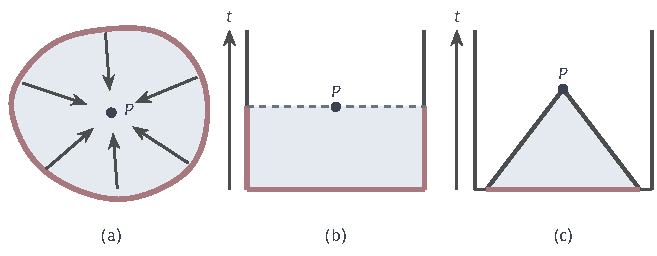
\includegraphics[width=111.3mm]{figures/06-differential-equations/02-partial-differential-equations/tikz/pdeprob-dependence/figure.pdf}
  \caption{内部点$P$的值依赖哪些数据（红）。(a)椭圆型：整个边界都影响$P$。(b)抛物型：时空图中，$P$之前的全部初值和侧面边值都影响$P$，浅蓝部分为依赖区域。(c)双曲型：只有深灰特征线所夹的底边影响$P$，这段红色底边之外的初值不起作用。}
  \label{fig:pdeprob-dependence}
\end{BookInlineFigure}

用点刺激可以把这种差别算出来。把总量为$1$的源或初值集中到一点，看三个方程的响应。在$(0,1)$上，两端为零、中点受单位点源的Poisson解是
\[
  u(x)=\frac12\min\{x,1-x\},
\]
它是一条折线，折点处斜率由$1/2$跳到$-1/2$，跳跃量$1$正好是点源的强度。解在整个区间上都不为零。

实轴上的热方程从原点的单位点热源出发，解是
\begin{equation}
  G(x,t)=\frac{1}{\sqrt{4\pi t}}\exp\Bigl(-\frac{x^{2}}{4t}\Bigr),\qquad t>0.
  \label{eq:pdeprob-heat-kernel}
\end{equation}
直接求导可以验证它满足方程：
\[
  \partial_tG=\partial_x^{2}G=\Bigl(\frac{x^{2}}{4t^{2}}-\frac{1}{2t}\Bigr)G.
\]
对任意$t>0$和任意$x$都有$G>0$，影响瞬间到达每一点，只是远处非常小。例如$x=1$，$t=0.01$时，$G\approx3.9\times10^{-11}$。

实轴上的波动方程以$c=1$、初位移为零、初速度为单位点刺激时，解是
\[
  u(x,t)=\frac12\mathbb{I}\{\lvert x\rvert<t\},
\]
影响的前沿以速度$1$前进，前沿之外严格为零。图~\ref{fig:pdeprob-point-response}并排画出了这三种响应。

\begin{BookInlineFigure}
  \centering
  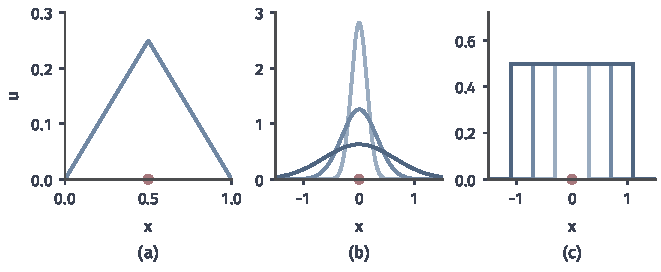
\includegraphics[width=112.0mm]{figures/06-differential-equations/02-partial-differential-equations/matplotlib/pdeprob-point-response/figure.pdf}
  \caption{对单位点刺激（红点）的响应。(a)$(0,1)$上的Poisson方程，解为折线。(b)实轴上的热方程，蓝色由浅到深为$t=0.01,0.05,0.2$，处处为正。(c)实轴上的波动方程，$c=1$，蓝色由浅到深为$t=0.3,0.7,1.1$，前沿之外为零。}
  \label{fig:pdeprob-point-response}
\end{BookInlineFigure}

表~\ref{tab:pdeprob-type-roles}汇总了这些差别，以及与之相配的数据。表中的结论是对模型方程而言的典型行为，一般方程要在相应条件下分别证明。

\begin{BookInlineTable}
  \centering
  \begin{tabular}{llll}
    \toprule
     & 椭圆型 & 抛物型 & 双曲型\\
    \midrule
    模型 & Poisson & 热 & 波动\\
    数据 & 全部边界 & 初值、侧面 & 两个初值、侧面\\
    传播 & 无时间方向 & 速度无穷 & 速度有限\\
    不光滑性 & 内部不产生 & 瞬间抹平 & 沿特征传播\\
    时间方向 & 无 & 不可逆 & 可逆\\
    \bottomrule
  \end{tabular}
  \caption{三类二阶模型方程的典型行为。}
  \label{tab:pdeprob-type-roles}
\end{BookInlineTable}

\paragraph{分类的适用范围}
类型是逐点定义的，系数随位置变化时类型可以改变。Tricomi方程$y\,\partial_x^{2}u+\partial_y^{2}u=0$的系数矩阵是$\operatorname{diag}(y,1)$：$y>0$时椭圆型，$y<0$时双曲型，$y=0$时退化。

在$y<0$的半平面，特征线满足$y\varphi_x^{2}+\varphi_y^{2}=0$，取$\varphi=x\mp\frac23(-y)^{3/2}$可以直接验证。图~\ref{fig:pdeprob-tricomi}中这两族曲线在下半平面交织，在$y=0$处形成尖点，上半平面没有特征线。这样的方程要在两个区域上分别提数据，不能套用单一类型的结论。

\begin{BookInlineFigure}
  \centering
  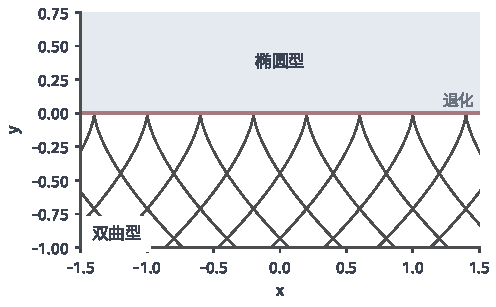
\includegraphics[width=84.0mm]{figures/06-differential-equations/02-partial-differential-equations/matplotlib/pdeprob-tricomi/figure.pdf}
  \caption{Tricomi方程$y\,\partial_x^2u+\partial_y^2u=0$的类型随位置变化。上半平面（浅蓝）椭圆型，红线$y=0$处退化，下半平面双曲型，深灰曲线是特征线$x\mp\frac23(-y)^{3/2}=$常数。}
  \label{fig:pdeprob-tricomi}
\end{BookInlineFigure}

分类也不记录变量的角色。方程$\partial_tu=\partial_x^{2}u$把$t$换成$-t$，得到$-\partial_tu=\partial_x^{2}u$，$\bm{M}$完全相同，仍是抛物型。但第一个方程向未来演化是好问题，向过去演化却不是，第~\ref{sec:pdeprob-well-posedness}节将具体算出差别。所以说一个方程是抛物型时，还要说明哪个变量是时间、沿哪个方向演化。

拟线性方程的主部系数依赖解，类型要在给定的解处判断，同一方程对不同的解可以不同。分类本身是线性方程的概念，推广到非线性方程总要先指明在哪个解上取线性化。

\paragraph{一阶方程按特征传播}
一阶方程没有二阶主部，二次型的分类对它们说不出什么，要改用另一种语言：信息沿曲线传递，这些曲线由常微分方程确定，同样称为特征线。

输运方程$\partial_tu+\bm{v}\cdot\nabla u=0$的特征线就是流体粒子的轨迹$\mathrm{d}\bm{x}/\mathrm{d}t=\bm{v}(\bm{x},t)$，它由给定的速度场决定，与解无关，沿线$u$不变。

非线性时情况改变。守恒律$\partial_tu+\partial_xF(u)=0$可以写成$\partial_tu+F'(u)\partial_xu=0$，信息的传播速度$F'(u)$依赖解本身，不同位置出发的曲线可能相交。Hamilton--Jacobi方程$\partial_tu+H(\nabla u)=0$对梯度非线性，沿曲线传递的是值和梯度，解在曲线相遇处会产生尖点。

这些方程的中心问题不是分类，而是相交之后如何选择解。这需要先搞清楚“解”究竟是什么意思。

\section{解的含义}
\label{sec:pdeprob-solutions}

到目前为止，“$u$满足方程”都是指把导数算出来、逐点代入。前面几个例子已经暴露了这种理解的局限：折线初值的折角在波动方程中一直存在，初值和边值不相容时输运方程的解带一条间断线。这些函数是不是解？要回答这个问题，就要明确“满足方程”的方式。

\paragraph{经典解}
最直接的要求是方程涉及的导数都存在且连续，方程逐点成立，初边值也逐点取到。

\begin{definition}[经典解]
\label{def:pdeprob-classical}
设$\Omega$是有界开集。Poisson方程$-\Delta u=f$配边值$u=g$的\term{经典解}（classical solution）是满足下列条件的函数：$u\in C^{2}(\Omega)\cap C(\overline{\Omega})$，在$\Omega$内每一点$-\Delta u=f$，在$\partial\Omega$上每一点$u=g$。对热方程问题~\eqref{eq:pdeprob-heat-ibvp}，经典解要求$u$对$\bm{x}$二阶、对$t$一阶连续可微于$\Omega\times(0,T]$，在$\overline{Q}$上连续，方程和初边值逐点成立。
\end{definition}

定义中的两层要求分工不同：内部的光滑性让方程有意义，到边界的连续性让边值有意义。热方程不要求光滑到$t=0$，正是为了容纳第~\ref{sec:pdeprob-initial}小节中的折线初值。

经典解的概念在两种情况下不够用：数据本身粗糙，或者解在演化中自己失去光滑性。下面逐一看。

\paragraph{粗糙的源项}
在$(0,1)$上考虑$-u''=f$，$u(0)=u(1)=0$，其中源项只在中间一段加热：
\begin{equation}
  f(x)=\begin{cases}4,&1/4<x<3/4,\\0,&\text{其他}.\end{cases}
  \label{eq:pdeprob-step-source}
\end{equation}
若$u\in C^{2}$，$u''$连续，但$u''=-f$在$x=1/4$处跳跃，所以经典解不存在。可是这根棒有确定的稳态温度，问题出在我们对“解”的要求太高。

分段把这个温度算出来。由对称性，$u'(1/2)=0$，所以在中段$u'(x)=-4(x-1/2)$，到左分界点时$u'(1/4)=1$。在$(0,1/4)$上$u''=0$，$u'$恒为$1$，由$u(0)=0$得
\[
  u(x)=x,\qquad 0\leq x\leq\frac14.
\]
中段积分一次得$u(x)=C-2(x-1/2)^{2}$，由$x=1/4$处连续，$C-\frac18=\frac14$，于是
\[
  u(x)=\frac38-2\Bigl(x-\frac12\Bigr)^{2},\qquad \frac14\leq x\leq\frac34.
\]
右段由对称性得$u(x)=1-x$。

这个函数在图~\ref{fig:pdeprob-weak-piecewise}中是一条光滑的曲线，$u$和$u'$都连续，只有$u''$在两个分界点跳跃。除这两点外方程逐点成立。我们希望有一种“解”的定义，能把它算进去，又不至于什么都算进去。

\begin{BookInlineFigure}
  \centering
  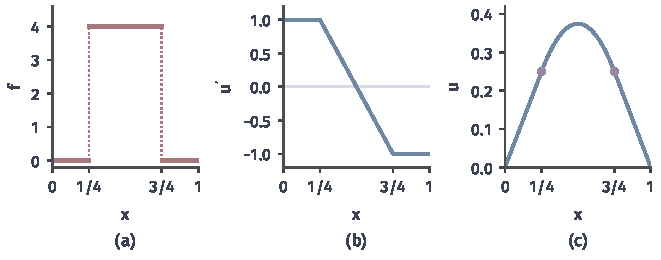
\includegraphics[width=112.0mm]{figures/06-differential-equations/02-partial-differential-equations/matplotlib/pdeprob-weak-piecewise/figure.pdf}
  \caption{跳跃源项下的解。(a)源项$f$，在$1/4$和$3/4$处跳跃。(b)$u'$连续，折点处$u''$跳跃。(c)$u$，紫点标出两个分界点，$u(1/2)=3/8$。}
  \label{fig:pdeprob-weak-piecewise}
\end{BookInlineFigure}

\paragraph{用测试函数检验}
把逐点检验换成加权平均的检验。逐点检验好比用一根无限细的探针逐点测量，而现实的探针总有一定宽度，读到的是附近的加权平均。两个函数相等，既可以逐点比较，也可以用所有光滑探针读数比较，后者不需要任何点上的导数。

设$\varphi$是\term{测试函数}（test function），即在$\Omega$内紧支撑的无穷次可微函数，全体记作$C_c^{\infty}(\Omega)$。若$u$是经典解，把$-\Delta u=f$乘以$\varphi$并在$\Omega$上积分，由分部积分得到
\[
  \int_\Omega\nabla u\cdot\nabla\varphi\,\mathrm{d}\bm{x}=\int_\Omega f\varphi\,\mathrm{d}\bm{x}.
\]
边界项因为$\varphi$在边界附近为零而消失。这个等式只含$u$的一阶导数，导数被挪了一阶到探针上。

把一阶导数也放宽，就要用到弱导数。设局部可积函数$w$对所有测试函数满足
\[
  \int_\Omega u\,\partial_{x_i}\varphi\,\mathrm{d}\bm{x}=-\int_\Omega w\,\varphi\,\mathrm{d}\bm{x},
\]
就称$w$是$u$的弱导数，这个$w$在几乎处处意义下唯一。详细的定义和性质可参考\BookChapterRef{chap:smoothing-weak-derivatives}{卷四第7章“光滑逼近与弱导数”}。

$H^{1}(\Omega)$由本身及各弱导数都属于$L^{2}(\Omega)$的函数组成，$H_0^{1}(\Omega)$是$C_c^{\infty}(\Omega)$在$H^{1}$范数下的闭包，在有界Lipschitz区域上恰好是边界迹为零的函数。这些空间的完备性、迹和嵌入性质可参考\BookChapterRef{chap:sobolev-spaces}{卷四第21章“Sobolev空间”}。

\begin{definition}[Poisson方程的弱解]
\label{def:pdeprob-weak-poisson}
设$\Omega\subset\mathbb{R}^{d}$是有界开集，$f\in L^{2}(\Omega)$。若$u\in H_0^{1}(\Omega)$满足
\begin{equation}
  \begin{gathered}
    a(u,v)=\int_\Omega fv\,\mathrm{d}\bm{x},\qquad\forall v\in H_0^{1}(\Omega),\\
    a(u,v)=\int_\Omega\nabla u\cdot\nabla v\,\mathrm{d}\bm{x},
  \end{gathered}
  \label{eq:pdeprob-weak-form}
\end{equation}
则称$u$是零边值Poisson问题的\term{弱解}（weak solution），式~\eqref{eq:pdeprob-weak-form}称为它的\term{弱形式}（weak formulation）。
\end{definition}

定义的三个成分各有作用。要求$u\in H^{1}$，式~\eqref{eq:pdeprob-weak-form}左边才有意义；要求$u\in H_0^{1}$，把零边值写进了解所在的空间；让$v$取遍$H_0^{1}$而非只取测试函数，并没有增加要求，因为测试函数在其中稠密、等式两边对$v$连续。

分段例子的$u$是弱解。$u$连续可微且在两端为零，所以$u\in H_0^{1}(0,1)$。对测试函数$\varphi$，把积分分成三段分别分部积分：
\[
  \int_0^{1}u'\varphi'\,\mathrm{d}x
  =\sum_{\text{三段}}\Bigl(\bigl[u'\varphi\bigr]-\int u''\varphi\,\mathrm{d}x\Bigr).
\]
$u'$在两个分界点连续，相邻两段的端点项互相抵消，$\varphi$在$0,1$处为零，端点项全部消失。各段内$-u''=f$，于是
\[
  \int_0^{1}u'\varphi'\,\mathrm{d}x=\int_0^{1}f\varphi\,\mathrm{d}x.
\]

弱解的要求并不是“几乎处处满足方程”。在$(0,1)$上取$f=0$，考虑折线$u=\min\{x,1-x\}$，除$x=1/2$外$u''=0$，两端也为零。它是不是$-u''=0$的弱解？取测试函数$\varphi$，同样分段，$u'$在$(0,1/2)$上是$1$，在$(1/2,1)$上是$-1$：
\[
  \int_0^{1}u'\varphi'\,\mathrm{d}x
  =\int_0^{1/2}\varphi'\,\mathrm{d}x-\int_{1/2}^{1}\varphi'\,\mathrm{d}x
  =2\varphi\Bigl(\frac12\Bigr).
\]

结果不为零，所以折线不是弱解：探针读出了折点。这个折点实际上是一个集中在$x=1/2$、强度为$2$的点热源，第~\ref{sec:pdeprob-types}节的点源解就是这一函数的一半。

图~\ref{fig:pdeprob-kink-test}取一个具体的光滑探针演示，(b)中$u'\varphi'$在两侧都是正的，面积加起来等于$2\varphi(1/2)=2$。“几乎处处”忽略了一点上发生的事，而测试函数不会。

\begin{BookInlineFigure}
  \centering
  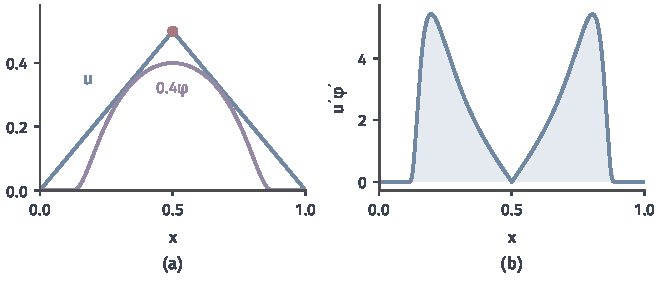
\includegraphics[width=112.0mm]{figures/06-differential-equations/02-partial-differential-equations/matplotlib/pdeprob-kink-test/figure.pdf}
  \caption{探针读出折点。(a)折线$u=\min\{x,1-x\}$（蓝，红点为折点）与测试函数$\varphi(x)=\exp(1-1/(1-r^2))$，$r=(x-\frac12)/0.4$（紫，图中缩放$0.4$倍）。(b)$u'\varphi'$，阴影面积的数值积分为$2.000$，等于$2\varphi(\frac12)$。}
  \label{fig:pdeprob-kink-test}
\end{BookInlineFigure}

弱解是经典解的推广，而不是另一种东西。下面的定理说明，函数足够光滑时两者一致。

\begin{theorem}[弱解与经典解的相容]
\label{thm:pdeprob-weak-classical}
设$\Omega$是有界Lipschitz区域，$f\in C(\overline{\Omega})$，$u\in C^{2}(\overline{\Omega})$且在$\partial\Omega$上$u=0$。则$u$是经典解，当且仅当$u$满足弱形式~\eqref{eq:pdeprob-weak-form}。
\end{theorem}

\begin{proof}
$u$连续可微到边界且边界值为零，所以$u\in H_0^{1}(\Omega)$。对$v\in C_c^{\infty}(\Omega)$，由乘积法则，
\[
  \nabla\cdot(v\nabla u)=\nabla v\cdot\nabla u+v\Delta u.
\]
$v$在边界附近为零，由散度定理，左边的积分为零，于是
\[
  \int_\Omega\nabla u\cdot\nabla v\,\mathrm{d}\bm{x}=-\int_\Omega v\,\Delta u\,\mathrm{d}\bm{x}.
\]

若$u$是经典解，右边等于$\int_\Omega fv\,\mathrm{d}\bm{x}$，对测试函数成立。式~\eqref{eq:pdeprob-weak-form}两边都是$v$在$H^{1}$范数下的连续线性泛函，由稠密性，等式对全部$v\in H_0^{1}(\Omega)$成立。

反过来，若弱形式成立，则对任意测试函数$v$有
\[
  \int_\Omega(-\Delta u-f)\,v\,\mathrm{d}\bm{x}=0.
\]
$-\Delta u-f$连续。若它在某点为正，取在该点附近非负、不恒为零的测试函数$v$，积分为正，矛盾；为负时同理。所以$-\Delta u=f$在$\Omega$内处处成立。
\end{proof}

\paragraph{演化产生的间断}
第二种情况更棘手：数据没有间断，解却在有限时间内失去光滑性。考虑守恒律$\partial_tu+\partial_x(u^{2}/2)=0$，即拟线性方程$\partial_tu+u\,\partial_xu=0$，通常称为Burgers方程。沿直线$x=x_0+u_0(x_0)t$，
\[
  \frac{\mathrm{d}}{\mathrm{d}t}u(x_0+u_0(x_0)t,t)=\partial_tu+u_0(x_0)\partial_xu=0.
\]
所以$u$沿这条直线保持初值$u_0(x_0)$，初值大的点跑得快。

取初值
\begin{equation}
  u_0(x)=\begin{cases}1,&x<0,\\1-x,&0\leq x\leq1,\\0,&x>1.\end{cases}
  \label{eq:pdeprob-burgers-ramp}
\end{equation}
由$x=x_0+(1-x_0)t$解出$x_0=(x-t)/(1-t)$，在$t<1$时得到
\[
  u(x,t)=\frac{1-x}{1-t},\qquad t\leq x\leq1.
\]
这时$\partial_xu=-1/(1-t)$，$t\to1$时斜率趋于无穷。图~\ref{fig:pdeprob-burgers-crossing}(a)中，从$[0,1]$出发的直线全部在$(1,1)$汇聚；(b)中坡面越来越陡，$t=1$时成为垂直的台阶。此后沿直线算出的值成为多值，方程必须换一种读法。斜坡的两个折角只是为了算得出显式解，把它磨成无穷次可微的初值，坡面同样会在有限时间变成垂直。

\begin{BookInlineFigure}
  \centering
  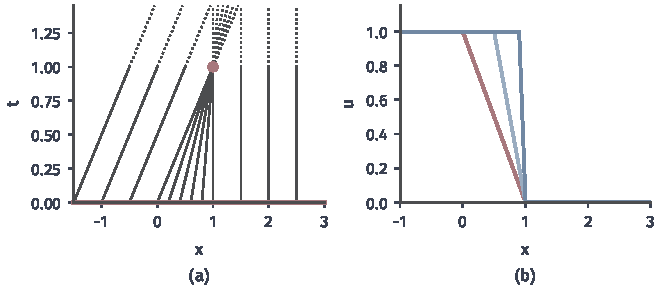
\includegraphics[width=112.0mm]{figures/06-differential-equations/02-partial-differential-equations/matplotlib/pdeprob-burgers-crossing/figure.pdf}
  \caption{Burgers方程的斜坡初值。(a)从初始线（红）出发的直线$x=x_0+u_0(x_0)t$（深灰），在红点$(1,1)$汇聚，虚线部分表示相交后已无法继续沿用。(b)解的形状，红线为$t=0$，蓝色由浅到深为$t=0.5,0.9$。}
  \label{fig:pdeprob-burgers-crossing}
\end{BookInlineFigure}

同样的办法可以用在这里，但必须从守恒形式出发。设$u$是光滑解，把$\partial_tu+\partial_xF(u)=0$乘以$\varphi\in C_c^{\infty}(\mathbb{R}\times[0,\infty))$，在$\mathbb{R}\times(0,\infty)$上积分并分部积分，所有导数都转到$\varphi$上：
\begin{equation}
  \int_0^{\infty}\!\!\int_{\mathbb{R}}\bigl(u\,\partial_t\varphi+F(u)\,\partial_x\varphi\bigr)\,\mathrm{d}x\,\mathrm{d}t
  +\int_{\mathbb{R}}u_0\,\varphi(\cdot,0)\,\mathrm{d}x=0.
  \label{eq:pdeprob-weak-conservation}
\end{equation}
$\varphi$在$t=0$可以不为零，第二项由此而来，初值由它写进方程。局部有界可测函数$u$若对所有这样的$\varphi$满足式~\eqref{eq:pdeprob-weak-conservation}，就称为守恒律的弱解。这个式子里没有$u$的导数，间断的$u$也可以代入。

必须强调从守恒形式出发。$u\,\partial_xu$在$u$间断时没有定义，而$\partial_x(u^{2}/2)$可以用弱导数理解。两种写法对光滑解等价，对间断解不等价。

线性方程的粗糙解也用同样的方式理解。输运方程带间断线的解~\eqref{eq:pdeprob-transport-solution}和波动方程带折角的解，都可以看成光滑解的极限；把导数全部转到测试函数上之后，积分等式在极限下保持成立，它们因此是弱解。这回答了本节开头的问题。

\paragraph{弱解可以不唯一}
放宽到这一步后，又出现了新问题。下面算出间断解需要满足的条件。设$u$在直线$x=st$左侧为常数$u_l$，右侧为常数$u_r$，初值是相应的台阶。在左侧区域上对向量场$(F(u_l)\varphi,u_l\varphi)$用散度定理，这个区域的边界由$t=0$的半直线和$x=st$组成，得到
\[
  \begin{aligned}
  &\iint_{x<st}\bigl(u_l\partial_t\varphi+F(u_l)\partial_x\varphi\bigr)\,\mathrm{d}x\,\mathrm{d}t\\
  &\qquad=\int_0^{\infty}\bigl(F(u_l)-su_l\bigr)\varphi(st,t)\,\mathrm{d}t
  -\int_{-\infty}^{0}u_l\varphi(x,0)\,\mathrm{d}x.
  \end{aligned}
\]
右侧区域的计算相同，只是直线上的外法向反号。两式相加，再加上式~\eqref{eq:pdeprob-weak-conservation}的初值项，初值积分全部抵消，只剩直线上的积分：
\[
  \int_0^{\infty}\bigl(F(u_l)-F(u_r)-s(u_l-u_r)\bigr)\varphi(st,t)\,\mathrm{d}t=0.
\]
对所有$\varphi$成立，当且仅当间断速度满足
\begin{equation}
  s\,(u_r-u_l)=F(u_r)-F(u_l).
  \label{eq:pdeprob-jump-condition}
\end{equation}

现在取Burgers方程，$F(u)=u^{2}/2$，初值在$x<0$时为$0$，$x>0$时为$1$。下面两个函数都是弱解。第一个是间断解：$u_l=0$，$u_r=1$，由式~\eqref{eq:pdeprob-jump-condition}，$s=\frac12$，
\[
  u^{\mathrm{a}}(x,t)=\begin{cases}0,&x<t/2,\\1,&x>t/2.\end{cases}
\]
第二个是连续的扇形：
\[
  u^{\mathrm{b}}(x,t)=\begin{cases}0,&x\leq0,\\x/t,&0<x<t,\\1,&x\geq t.\end{cases}
\]
扇形内部$\partial_tu+u\,\partial_xu=-x/t^{2}+(x/t)(1/t)=0$，它在两条分界线上连续，分段积分时端点项抵消，所以也满足式~\eqref{eq:pdeprob-weak-conservation}。

一个初值对应两个弱解，弱形式提供的信息不足以挑出一个。图~\ref{fig:pdeprob-riemann}(a)中，$u^{\mathrm{a}}$两侧的特征线都从间断处发出，好比信息从间断线上凭空产生，这在物理上不合理；(b)中的$u^{\mathrm{b}}$没有这个问题。(c)给方程加上一个很小的黏性项，算出来的解贴近$u^{\mathrm{b}}$。

\begin{BookInlineFigure}
  \centering
  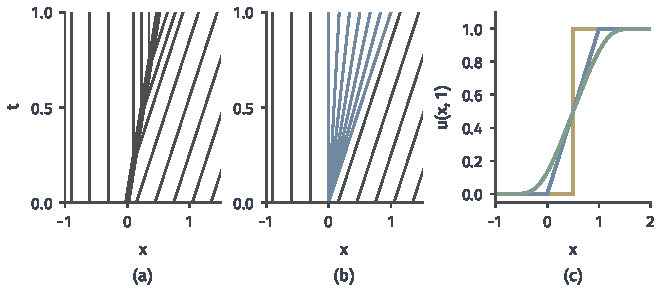
\includegraphics[width=112.0mm]{figures/06-differential-equations/02-partial-differential-equations/matplotlib/pdeprob-riemann/figure.pdf}
  \caption{同一台阶初值的两个弱解。(a)间断解：深灰粗线是间断线$x=t/2$，细线是特征线，它们都从间断线离开。(b)扇形解：蓝线是从原点发出的扇形特征线。(c)$t=1$的形状：间断解（黄）、扇形解（蓝）、带黏性$\nu=0.02$的数值解（绿）。}
  \label{fig:pdeprob-riemann}
\end{BookInlineFigure}

要恢复唯一性，就要在弱解中增加一条选择规则，只保留与小黏性极限一致的解。满足这种规则的弱解称为\term{熵解}（entropy solution），第~\ref{chap:scalar-conservation-laws}章给出精确的定义并证明唯一性。

\paragraph{Hamilton--Jacobi方程：几乎处处太宽}
最后一种情况说明，弱导数的办法并不总能用上。考虑$\lvert u'\rvert=1$，$x\in(-1,1)$，$u(\pm1)=0$，这是从边界出发、速度为$1$的波前的到达时间所满足的方程。

它没有$C^{1}$解。若$u\in C^{1}$，由Rolle定理存在一点$u'=0$，与$\lvert u'\rvert=1$矛盾。若只要求几乎处处成立，又有太多的解：图~\ref{fig:pdeprob-eikonal}(a)中每一条锯齿线的斜率都是$\pm1$，可以折任意多次。

这里不能把导数转到测试函数上，因为方程对$u'$非线性，$\lvert u'\rvert$无法通过分部积分移走。可行的选择办法仍然是加小黏性。考虑
\[
  (u')^{2}-\varepsilon u''=1,\qquad u(\pm1)=0.
\]
它有显式解
\begin{equation}
  u_\varepsilon(x)=\varepsilon\Bigl(\ln\cosh\frac{1}{\varepsilon}-\ln\cosh\frac{x}{\varepsilon}\Bigr).
  \label{eq:pdeprob-viscous-eikonal}
\end{equation}

下面验证。两次求导得到
\[
  u_\varepsilon'=-\tanh\frac{x}{\varepsilon},\qquad
  u_\varepsilon''=-\frac{1}{\varepsilon}\operatorname{sech}^{2}\frac{x}{\varepsilon}.
\]
于是
\[
  (u_\varepsilon')^{2}-\varepsilon u_\varepsilon''=\tanh^{2}\frac{x}{\varepsilon}+\operatorname{sech}^{2}\frac{x}{\varepsilon}=1.
\]
边值也满足，因为$\cosh$是偶函数。令$\varepsilon\to0$，由$\cosh s\approx\frac12\mathrm{e}^{\lvert s\rvert}$（$\lvert s\rvert$很大时），
\[
  \varepsilon\ln\cosh\frac{x}{\varepsilon}\to\lvert x\rvert,
\]
所以$u_\varepsilon\to1-\lvert x\rvert$。这正是到边界的距离，即波前的最短到达时间。图~\ref{fig:pdeprob-eikonal}(b)显示了这个极限。

\begin{BookInlineFigure}
  \centering
  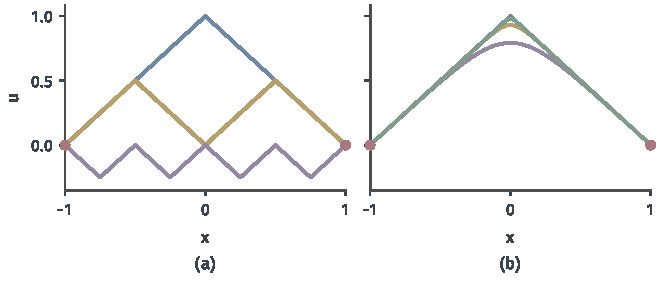
\includegraphics[width=112.0mm]{figures/06-differential-equations/02-partial-differential-equations/matplotlib/pdeprob-eikonal/figure.pdf}
  \caption{$\lvert u'\rvert=1$，$u(\pm1)=0$（红点）。(a)几个几乎处处满足方程的函数：$1-\lvert x\rvert$（蓝）和两条锯齿线（黄、紫）。(b)小黏性解$u_\varepsilon$，$\varepsilon=0.3$（紫）、$0.1$（黄）、$0.03$（绿）趋于$1-\lvert x\rvert$（蓝）。}
  \label{fig:pdeprob-eikonal}
\end{BookInlineFigure}

注意$\varepsilon$前的符号决定了选中的解：把$-\varepsilon u''$换成$+\varepsilon u''$，极限就成了$\lvert x\rvert-1$。这条选择规则的严格形式不用导数，而是在解被光滑函数从上方或下方触碰的点上提出不等式，满足它的解称为\term{黏性解}（viscosity solution），第~\ref{chap:hamilton-jacobi-equations}章专门讨论。

表~\ref{tab:pdeprob-solution-concepts}对比了这几种解的概念。它们不是彼此竞争的定义，而是针对不同方程结构的不同检验方式，光滑时都回到经典解。

\begin{BookInlineTable}
  \centering
  \begin{tabular}{lll}
    \toprule
    解的概念 & 检验方式 & 用在哪里\\
    \midrule
    经典解 & 逐点代入导数 & 数据和解都足够光滑\\
    弱解 & 导数转到测试函数上 & 方程有散度结构\\
    熵解 & 弱解，加熵条件 & 标量守恒律\\
    黏性解 & 用光滑函数从两侧触碰 & Hamilton--Jacobi方程\\
    \bottomrule
  \end{tabular}
  \caption{几种解的概念。}
  \label{tab:pdeprob-solution-concepts}
\end{BookInlineTable}

\section{适定性}
\label{sec:pdeprob-well-posedness}

写出一个公式，是否就解决了问题？细棒的热方程反向求解也有“公式”：把初值的正弦系数乘上一个增长的指数，形式上和正向完全对称。下面会看到，这个公式几乎没有用处。判断一个问题是否提得合理，需要把三个问题分开回答。

\paragraph{三个问题}
把问题看成从数据到解的一个映射。这个映射要有意义，至少要回答：对给定的数据，解存在吗？解只有一个吗？数据有小的误差时，解的变化也小吗？这三个问题只有在明确了数据和解分别属于什么空间、用什么范数度量之后，才有确切的答案。

\begin{definition}[适定问题]
\label{def:pdeprob-well-posed}
设数据空间$D$和解空间$S$是赋范空间。若对每个$d\in D$，问题在$S$中存在唯一的解$\mathcal{S}(d)$，且映射$\mathcal{S}:D\to S$连续，即
\begin{equation}
  \lVert d_n-d\rVert_{D}\to0\ \Longrightarrow\ \lVert\mathcal{S}(d_n)-\mathcal{S}(d)\rVert_{S}\to0,
  \label{eq:pdeprob-continuous-dependence}
\end{equation}
就称问题在$(D,S)$下是\term{适定问题}（well-posed problem），否则称为\term{不适定问题}（ill-posed problem）。
\end{definition}

这是Hadamard提出的标准。线性问题中$\mathcal{S}$是线性映射，连续性等价于存在常数$C$，使得
\[
  \lVert\mathcal{S}(d)\rVert_{S}\leq C\lVert d\rVert_{D},\qquad\forall d\in D.
\]

图~\ref{fig:pdeprob-well-posed-map}画出了这三条要求：每个数据都有箭头指出（存在），箭头只有一支（唯一），数据的邻域映到解的小邻域（连续依赖）。线性算子方程的相应结论，可参考\BookChapterRef{chap:linear-operator-equations}{卷四第19章“线性算子方程”}。

\begin{BookInlineFigure}
  \centering
  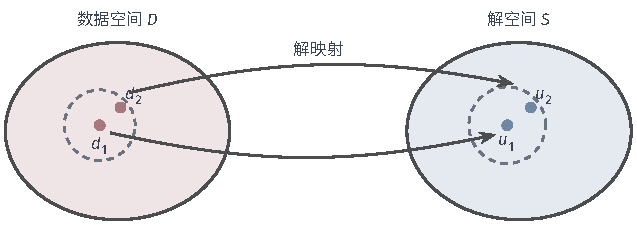
\includegraphics[width=107.8mm]{figures/06-differential-equations/02-partial-differential-equations/tikz/pdeprob-well-posed-map/figure.pdf}
  \caption{适定性是从数据空间到解空间的连续映射。虚线圈分别表示所选范数下的邻域，相近的数据$d_1,d_2$对应相近的解$u_1,u_2$。换一对空间，三条要求的答案都可能改变。}
  \label{fig:pdeprob-well-posed-map}
\end{BookInlineFigure}

\paragraph{存在：解空间是否够大}
存在性的答案依赖解空间。跳跃源项~\eqref{eq:pdeprob-step-source}在$C^{2}$中没有解，在$H_0^{1}$中有解；Neumann问题在数据违反式~\eqref{eq:pdeprob-neumann-compat}时哪里都没有解，这时要把数据空间缩小到满足约束的子空间。

非线性方程的存在性还有时间范围的问题。对Burgers方程，沿直线$x=x_0+u_0(x_0)t$，对$x_0$求导可得
\[
  \partial_xu=\frac{u_0'(x_0)}{1+u_0'(x_0)\,t}.
\]
只要某处$u_0'<0$，分母就会在有限时间变为零，光滑解只能存在到
\begin{equation}
  T^{*}=-\frac{1}{\min_xu_0'(x)}.
  \label{eq:pdeprob-burgers-breaking}
\end{equation}
式~\eqref{eq:pdeprob-burgers-ramp}的斜坡初值中$\min u_0'=-1$，$T^{*}=1$，与图~\ref{fig:pdeprob-burgers-crossing}一致。在$C^{1}$中只有局部解，放宽到弱解后解可以延续到所有时间。这和第~\ref{chap:ode-existence-continuation}章的情形类似，那里常微分方程的解也可能在有限时间爆炸，不过这里爆炸的是导数，而解本身仍然有界。

\paragraph{唯一：解空间是否够小}
解空间放得太大，唯一性就会失去，上一节的两个弱解和无穷多条锯齿线都是例子。Neumann问题差一个常数，这时要在解空间上加均值为零的条件，或者把差常数的函数视为同一个。

对线性演化方程，证明唯一性最常用的工具是能量估计：对两个解的差构造一个非负量，证明它不增。下面的定理同时给出唯一性和连续依赖。

\begin{theorem}[细棒热方程的能量估计]
\label{thm:pdeprob-heat-energy}
设$u_1,u_2$在$[0,1]\times[0,T]$上连续，$\partial_tu_i$、$\partial_xu_i$、$\partial_x^{2}u_i$在同一闭集上连续，满足同一方程$\partial_tu=\partial_x^{2}u+f$和同一边值$u(0,t)=g_0(t)$、$u(1,t)=g_1(t)$。则对$t\in[0,T]$，
\begin{equation}
  \lVert u_1(\cdot,t)-u_2(\cdot,t)\rVert_{L^{2}(0,1)}\leq\lVert u_1(\cdot,0)-u_2(\cdot,0)\rVert_{L^{2}(0,1)}.
  \label{eq:pdeprob-heat-energy}
\end{equation}
特别地，初值相同的两个解相等。
\end{theorem}

\begin{proof}
记$w=u_1-u_2$。由线性，$w$满足$\partial_tw=\partial_x^{2}w$，两端值为零。定义
\[
  E(t)=\frac12\int_0^{1}w(x,t)^{2}\,\mathrm{d}x.
\]
$\partial_tw$在闭集上连续，可以在积分号下求导，再代入方程：
\[
  E'(t)=\int_0^{1}w\,\partial_tw\,\mathrm{d}x=\int_0^{1}w\,\partial_x^{2}w\,\mathrm{d}x.
\]
分部积分，端点项$[w\,\partial_xw]_0^{1}$因$w$在两端为零而消失：
\[
  E'(t)=-\int_0^{1}(\partial_xw)^{2}\,\mathrm{d}x\leq0.
\]
所以$E(t)\leq E(0)$，开方即得式~\eqref{eq:pdeprob-heat-energy}。初值相同时$E(0)=0$，于是$E\equiv0$，$w\equiv0$。
\end{proof}

定理中的条件要求解光滑到初始时刻和边界。在无界区域上，单凭方程和初值并不能保证唯一性：实轴上的热方程存在初值为零、但不恒为零的解，它们在$\lvert x\rvert\to\infty$时增长得极快。这个构造由Tikhonov给出，证明需要较长的级数估计，读者可查阅偏微分方程教材。加上增长限制$\lvert u(x,t)\rvert\leq C\mathrm{e}^{ax^{2}}$后唯一性恢复，这说明解空间的限制不是技术细节。

\paragraph{连续依赖：同一方程，两个方向}
现在回到本节开头的问题。设$u_0=\sum_kb_k\sin k\pi x$，$u$是细棒两端为零的热方程的解，则第$k$个模式的系数在时刻$t$变为$b_k\mathrm{e}^{-k^{2}\pi^{2}t}$。由正弦函数的正交性，$\lVert\sin k\pi x\rVert_{L^{2}(0,1)}^{2}=\frac12$，于是
\[
  \lVert u(\cdot,T)\rVert_{L^{2}(0,1)}^{2}
  =\frac12\sum_kb_k^{2}\mathrm{e}^{-2k^{2}\pi^{2}T}
  \leq\lVert u_0\rVert_{L^{2}(0,1)}^{2}.
\]
正向映射$u_0\mapsto u(\cdot,T)$在$L^{2}$上有界，高频模式被强烈衰减。

反过来，由$T$时刻的温度$d=\sum_kd_k\sin k\pi x$推算初始温度，公式也可以写出来：
\begin{equation}
  u(x,0)=\sum_{k\geq1}d_k\,\mathrm{e}^{k^{2}\pi^{2}T}\sin k\pi x.
  \label{eq:pdeprob-backward-heat}
\end{equation}
形式上它和正向一样简单，但指数的符号反了。图~\ref{fig:pdeprob-backward-heat}(a)比较了两个方向上各模式的放大倍数。

这个公式首先不保证解存在。要让式~\eqref{eq:pdeprob-backward-heat}属于$L^{2}$，$d_k$必须满足$\sum_kd_k^{2}\mathrm{e}^{2k^{2}\pi^{2}T}<\infty$。折线$\min\{x,1-x\}$的系数只有$k^{-2}$的量级，不满足这个条件，它不可能是任何$L^{2}$初值在正时刻的温度。这和正向热方程瞬间变光滑是同一件事。

唯一性倒还成立：若$d=0$，每个$d_k$为零，$L^{2}$初值的所有系数都为零。问题出在连续依赖。取数据的扰动$\delta=\varepsilon\sin k\pi x$，它的$L^{2}$范数是$\varepsilon/\sqrt{2}$，反算出的初值扰动是
\[
  \varepsilon\,\mathrm{e}^{k^{2}\pi^{2}T}\sin k\pi x,
\]
放大倍数是$\mathrm{e}^{k^{2}\pi^{2}T}$，随$k$无界增长。所以反向映射在$L^{2}$上无界，问题在$(L^{2},L^{2})$下不适定。

下面取具体的数字。$T=0.1$，真实初值$\sin\pi x$，它在$T$时刻的温度是$\mathrm{e}^{-\pi^{2}T}\sin\pi x$。给这个数据加上幅度$\varepsilon=10^{-10}$的第$5$模式扰动，反算时模式$5$的放大倍数是
\[
  \mathrm{e}^{25\pi^{2}\cdot0.1}\approx5.2\times10^{10},
\]
反算结果中出现幅度约$5.2$的振荡。图~\ref{fig:pdeprob-backward-heat}(b)中，真实解的幅度为$1$，几乎完全被这个振荡淹没，而数据的扰动只有$10^{-10}$，小于任何测量误差。

\begin{BookInlineFigure}
  \centering
  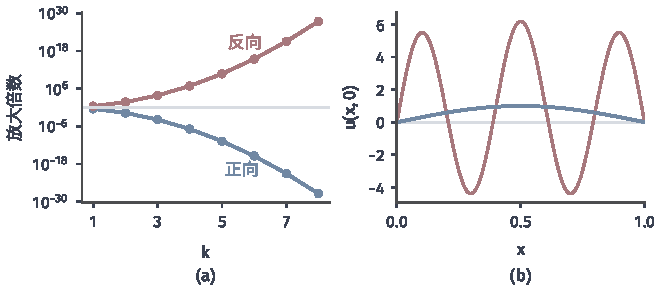
\includegraphics[width=112.0mm]{figures/06-differential-equations/02-partial-differential-equations/matplotlib/pdeprob-backward-heat/figure.pdf}
  \caption{热方程的两个方向，$T=0.1$。(a)第$k$个模式的放大倍数：正向$\mathrm{e}^{-k^2\pi^2T}$（蓝）与反向$\mathrm{e}^{k^2\pi^2T}$（红），纵轴为对数坐标。(b)真实初值$\sin\pi x$（蓝）与数据含幅度$10^{-10}$的第$5$模式扰动时的反算结果（红）。}
  \label{fig:pdeprob-backward-heat}
\end{BookInlineFigure}

适定性是相对于空间而言的，这里可以看得很清楚。若把数据空间的范数改为
\[
  \lVert d\rVert_{*}^{2}=\frac12\sum_kd_k^{2}\mathrm{e}^{2k^{2}\pi^{2}T},
\]
反向映射就成了等距映射，问题“适定”了。但这个范数下的小，意味着高频分量小到指数级，现实的测量误差达不到，这种适定性没有实用价值。选择空间时要问：数据的误差实际上在什么范数下小？

\paragraph{同一方程，换一种数据}
椭圆方程有一个著名的类似例子，说明同一方程配不同的数据，结果可以完全不同。考虑上半平面上的Laplace方程，把$y$当作“时间”，像波动方程那样给两个初值：
\begin{equation}
  \partial_x^{2}u+\partial_y^{2}u=0,\qquad
  u(x,0)=0,\qquad \partial_yu(x,0)=\frac{\sin kx}{k}.
  \label{eq:pdeprob-hadamard}
\end{equation}
直接代入可以验证，解是
\[
  u(x,y)=\frac{\sinh(ky)\sin kx}{k^{2}}.
\]

$k\to\infty$时，数据一致地趋于零，解却对每个$y>0$都按$\mathrm{e}^{ky}/(2k^{2})$爆炸。$k=20$时，数据的幅度只有$0.05$，在$y=1$处解的幅度是$\sinh(20)/400\approx6.1\times10^{5}$。图~\ref{fig:pdeprob-hadamard}画出了这种增长。若把数据换成$\sin(kx)/k^{m}$，数据的任意有限阶导数都趋于零，指数增长依然如故。

\begin{BookInlineFigure}
  \centering
  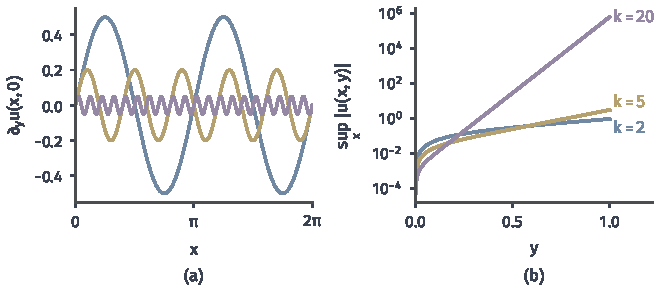
\includegraphics[width=112.0mm]{figures/06-differential-equations/02-partial-differential-equations/matplotlib/pdeprob-hadamard/figure.pdf}
  \caption{Laplace方程的“初值”问题~\eqref{eq:pdeprob-hadamard}。(a)数据$\partial_yu(x,0)=\sin(kx)/k$，$k=2$（蓝）、$5$（黄）、$20$（紫），频率越高幅度越小。(b)解的幅度$\sinh(ky)/k^2$随$y$的增长，纵轴为对数坐标。频率最高的数据最小，增长最快。}
  \label{fig:pdeprob-hadamard}
\end{BookInlineFigure}

同一方程配Dirichlet数据却是适定的。在$(0,1)$上取$-u''=f$，$u(0)=u(1)=0$，先对解本身做能量估计。将方程乘以$u$并分部积分，端点项消失：
\[
  \lVert u'\rVert_{L^{2}}^{2}=\int_0^{1}fu\,\mathrm{d}x\leq\lVert f\rVert_{L^{2}}\lVert u\rVert_{L^{2}}.
\]
再把$u$展开成正弦级数$\sum_kc_k\sin k\pi x$，由$k\geq1$，
\[
  \lVert u'\rVert_{L^{2}}^{2}=\frac12\sum_kk^{2}\pi^{2}c_k^{2}\geq\pi^{2}\lVert u\rVert_{L^{2}}^{2},
\]
这是区间上的Poincaré不等式。把它代入上式右端，两边约去$\lVert u'\rVert_{L^{2}}$，得到
\begin{equation}
  \lVert u'\rVert_{L^{2}(0,1)}\leq\frac{1}{\pi}\lVert f\rVert_{L^{2}(0,1)}.
  \label{eq:pdeprob-poisson-energy}
\end{equation}
取$u=\sin\pi x$，$f=\pi^{2}\sin\pi x$时，两边都是$\pi/\sqrt{2}$，等号成立。由线性，这个估计同时给出唯一性和对$f$的连续依赖，存在性由第~\ref{chap:elliptic-equations}章的变分方法给出。

波动方程的估计量不同。设$u$在$[0,1]\times[0,T]$上二阶连续可微，满足$\partial_t^{2}u=c^{2}\partial_x^{2}u$和零边值，定义能量
\[
  E(t)=\frac12\int_0^{1}\bigl((\partial_tu)^{2}+c^{2}(\partial_xu)^{2}\bigr)\,\mathrm{d}x.
\]
求导并对第二项分部积分，端点上$\partial_tu=0$，于是
\begin{equation}
  E'(t)=\int_0^{1}\partial_tu\,\bigl(\partial_t^{2}u-c^{2}\partial_x^{2}u\bigr)\,\mathrm{d}x=0.
  \label{eq:pdeprob-wave-energy}
\end{equation}
能量守恒，对时间的两个方向都成立，这正是波动方程可逆的反映。它要求数据是一对函数，数据空间自然取$H_0^{1}(0,1)\times L^{2}(0,1)$，而不是$L^{2}$。

\paragraph{不同数据要求下的结果}
表~\ref{tab:pdeprob-well-posed-summary}把本章的例子放在一起。前两行方程相同、方向相反，第三、四行方程相同、数据位置不同，每一行都要连同空间一起读。其中Laplace方程Cauchy问题的唯一性来自调和函数的解析性，Burgers方程熵解的结论在第~\ref{chap:scalar-conservation-laws}章讨论，这里只记录结果。

\begin{BookInlineTable}
  \centering
  \begin{tabular}{llll}
    \toprule
    问题与空间 & 存在 & 唯一 & 连续依赖\\
    \midrule
    热方程正向，$L^{2}$ & 有 & 有 & 有\\
    热方程反向，$L^{2}$ & 一般无 & 有 & 无\\
    Poisson，Dirichlet，$H_0^{1}$ & 有 & 有 & 有\\
    Laplace，Cauchy数据 & 一般无 & 有 & 无\\
    Poisson，Neumann & 需式~\eqref{eq:pdeprob-neumann-compat} & 差常数 & 商掉常数后有\\
    Burgers，$C^{1}$ & 仅到$T^{*}$ & 有 & 局部有\\
    Burgers，弱解 & 有 & 无 & 无从谈起\\
    Burgers，熵解 & 有 & 有 & 有\\
    \bottomrule
  \end{tabular}
  \caption{同一方程在不同数据与空间要求下的适定性。}
  \label{tab:pdeprob-well-posed-summary}
\end{BookInlineTable}

适定也不等于计算容易。连续依赖只说误差放大倍数有限，这个倍数可能很大；离散后的方程是否继承连续问题的稳定性，是另一个问题，要在第~\ref{chap:pde-numerical-methods}章对具体格式讨论。

\section{本章小结}
\label{sec:pdeprob-summary}

一个偏微分方程问题由四样东西共同构成：未知场和它所在的区域，方程本身，初值和边界数据，以及“解”的含义和相应的函数空间。只写一条方程不等于提出了问题，$\partial_tu=\partial_x^{2}u$有无穷多解，它们的差别要由数据来确定。

未知量从向量变成函数后，方程可以由局部守恒和具体的通量规律得出，Poisson、输运、热和波动四个模型都写成同一组变量。空间离散后，热方程就是常微分方程组，但矩阵的谱范数按$4/h^{2}$增长，所以不能把常微分方程的存在性定理直接搬过来。

需要什么数据由方程决定。时间阶数决定初始函数的个数，边界条件可以规定场值、通量或两者的组合，输运方程只在入流边界给数据。初值与边值在角点要相容，相容的阶数随所要求的光滑性增加；Neumann问题还有积分约束。不是数据越多越好。

对二阶线性方程，系数矩阵特征值的符号结构决定类型：椭圆型受整个边界约束，抛物型立刻抹平，双曲型以有限速度传播不光滑性。类型在坐标变换下不变，但是逐点定义，也不记录时间的方向。一阶方程不在这个分类中，它们按特征线传播，非线性时特征线会相交。

数据粗糙或演化产生间断时，要改变方程成立的方式。弱解把导数转移到测试函数上；守恒律的弱解可以不唯一，要由熵解选择；Hamilton--Jacobi方程几乎处处意义下有太多解，要由黏性解选择。不同方程需要不同的解的概念，光滑时它们都回到经典解。

存在、唯一和连续依赖是三个要分别回答的问题，答案依赖所选的空间。热方程正向适定、反向不适定，Laplace方程配Dirichlet数据适定、配Cauchy数据不适定，公式形式上都写得出来，所以写出解不等于证明问题适定。本章的结论都是有限时间内的。

后面几章在具体模型中落实这些条件：第~\ref{chap:elliptic-equations}章建立椭圆方程的弱形式和适定性，第~\ref{chap:diffusion-equations}章和第~\ref{chap:wave-equations}章分别讨论抛物型和双曲型的演化，第~\ref{chap:transport-equations}章、第~\ref{chap:scalar-conservation-laws}章和第~\ref{chap:hamilton-jacobi-equations}章处理一阶方程及其解的选择，数值稳定性留到第~\ref{chap:pde-numerical-methods}章的离散问题中讨论。


\chapter{椭圆方程}
\label{chap:elliptic-equations}

一块金属板的边缘保持固定温度，板内某些地方持续发热。足够久之后，温度不再变化。板上每一点的温度是多少？这个数不能只看这一点附近：边缘上任何一段的温度升高，源项在任何一处的增强，都会让板内处处的温度发生变化。平衡场的每个值都同时取决于整个区域的数据。

这种“牵一发而动全身”的结构决定了椭圆方程的提法和做法。它没有时间方向，不能从一个初始时刻往后推，只能在整个区域上一次解出来。数据必须放在边界上，而且边界条件的类型决定了问题是否可解，也决定了解是否唯一。

能写出解的情形只占少数，但它们把结构摆得最清楚。区间上积分两次，就能看到积分常数怎样被边界条件吃掉；Green函数告诉我们一处的点源在别处产生多大的响应；特征函数把求解变成逐个模式的除法，还会暴露零特征值这个危险的情形。这些计算都要求解足够光滑，而系数有间断、源项很粗糙时，经典意义下的解根本不存在。

于是要换一种提法：不再逐点要求方程成立，而是要求方程经过所有测试函数检验后成立。这样得到的弱形式把二阶方程变成一阶导数的积分关系，边界条件也分成了写进空间和写进积分两种。Lax--Milgram定理随后给出存在、唯一和连续依赖，只是三类边界条件要用不同的方式验证它的条件。

最后三节从三个方向审视弱解：对称问题的弱解是能量的极小点，方程的符号结构给出最大值原理，系数和区域足够好时弱解还会更光滑。第~\ref{chap:diffusion-equations}章的扩散方程会沿用这里的空间和边界模式，空间离散放在第~\ref{chap:pde-numerical-methods}章。

\section{边值问题}
\label{sec:ellip-bvp}

一根细棒两端浸在冰水里，棒内各处均匀发热。温度稳定之后是什么样子？棒上任何一小段都处在收支平衡中：流进来的热量加上这一段自己产生的热量，等于流出去的热量。这个平衡关系就是方程的来源。

\paragraph{区间上的平衡}
设棒占据区间$(0,1)$，$u(x)$是稳定后的温度，$f(x)$是单位长度上的发热率，$q(x)$是$x$处向右流过的热流。取一小段$[x,x+\delta]$，如图~\ref{fig:ellip-flux-balance}(a)。稳态时这一段的热量不变，流出减流入等于内部产热：
\[
 q(x+\delta)-q(x)=\int_x^{x+\delta}f(s)\,\mathrm{d}s .
\]

两边除以$\delta$，令$\delta\to0$，得到$q'=f$。再用导热定律把热流与温度联系起来：热量从高温流向低温，流量正比于温度梯度，比例系数$a(x)>0$是导热率，即$q=-a\,u'$。代入后得到
\begin{equation}
 -\bigl(a(x)\,u'(x)\bigr)'=f(x),\qquad x\in(0,1).
 \label{eq:ellip-1d-equation}
\end{equation}

\begin{BookInlineFigure}
  \centering
  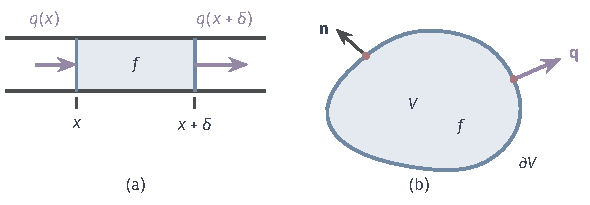
\includegraphics[width=100mm]{figures/06-differential-equations/02-partial-differential-equations/tikz/ellip-flux-balance/figure.pdf}
  \caption{热量收支平衡。(a)区间上的一小段：从左端流入$q(x)$，从右端流出$q(x+\delta)$，两者之差由段内的源项$f$补足。(b)多维区域中的控制体$V$：紫色箭头是热流$\bm{q}$，黑色箭头是边界的外法向$\bm{n}$，穿过$\partial V$的净流出量等于$V$内的总产热。}
  \label{fig:ellip-flux-balance}
\end{BookInlineFigure}

式~\eqref{eq:ellip-1d-equation}是二阶常微分方程，但它的提法与第~\ref{chap:ordinary-differential-equations}章的初值问题不同。初值问题在同一点给出$u$和$u'$，解可以从左向右递推。这里的两个条件分别放在区间的两端，右端的温度会影响左端，无法从一头推到另一头，必须把整段一起解出来。

取$a=1$、$f=1$，两端温度为零。方程$-u''=1$的解是
\begin{equation}
 u(x)=\frac{x(1-x)}{2},
 \label{eq:ellip-running-solution}
\end{equation}
它在中点取最大值$u(1/2)=1/8$。这个例子贯穿全章。后面每种方法算出的结果，都可以拿它来核对。

\paragraph{多维的散度型方程}
把收支平衡搬到区域$\Omega\subset\mathbb{R}^{d}$上。热流现在是向量场$\bm{q}(\bm{x})$，任取控制体$V\subset\Omega$，如图~\ref{fig:ellip-flux-balance}(b)，净流出量等于总产热：
\[
 \int_{\partial V}\bm{q}\cdot\bm{n}\,\mathrm{d}S=\int_Vf\,\mathrm{d}\bm{x} .
\]

由散度定理（可参考\BookChapterRef{chap:integral-theorems}{卷二第27章“积分定理”}），左端等于$\int_V\nabla\cdot\bm{q}\,\mathrm{d}\bm{x}$。这个等式对每个小控制体都成立，被积函数连续时可得$\nabla\cdot\bm{q}=f$。

导热率在不同方向上可能不同，例如木材顺纹与横纹导热差别很大，所以导热定律写成$\bm{q}=-\bm{A}(\bm{x})\nabla u$，其中$\bm{A}(\bm{x})$是$d\times d$的\term{扩散系数矩阵}（diffusion coefficient matrix）。于是得到散度型方程
\begin{equation}
 -\nabla\cdot\bigl(\bm{A}(\bm{x})\nabla u\bigr)=f\qquad\text{于}\ \Omega.
 \label{eq:ellip-divergence-form}
\end{equation}

取$\bm{A}=\bm{I}$，方程化为\term{Poisson方程}（Poisson equation）
\begin{equation}
 -\Delta u=f\qquad\text{于}\ \Omega,
 \label{eq:ellip-poisson}
\end{equation}
其中$\Delta u=\sum_{i=1}^d\partial_{i}^2u$是Laplace算子。$f=0$时称为Laplace方程，它的解称为\term{调和函数}（harmonic function）。方程前面的负号让$f>0$对应发热：$-\Delta u>0$表示$u$在该点附近比周围的平均值高，这正是热源处温度的样子。

第~\ref{chap:pde-problems}章按二阶项系数的符号结构区分方程类型：系数矩阵对称正定是椭圆型，还有一个时间方向上的一阶导数是抛物型，时间与空间的二阶导数异号是双曲型。式~\eqref{eq:ellip-divergence-form}没有时间，$\bm{A}$正定，就是椭圆型的典型代表。

\paragraph{三类边界条件}
方程只说明区域内部的收支，边界上发生什么要另外指定。设$\Omega$有界，$\bm{n}$是$\partial\Omega$上的外法向，$g$是边界上给定的函数。常用的条件有三类：

\begin{itemize}
 \item \term{Dirichlet边界条件}（Dirichlet boundary condition）$u=g$：边界温度由外界固定，如贴在恒温槽上。
 \item \term{Neumann边界条件}（Neumann boundary condition）$\bm{n}\cdot\bm{A}\nabla u=g$：规定穿过边界流入的热流。由$\bm{q}=-\bm{A}\nabla u$，$-\bm{q}\cdot\bm{n}$是单位面积上的流入量，$g=0$表示绝热。
 \item \term{Robin边界条件}（Robin boundary condition）$\bm{n}\cdot\bm{A}\nabla u+\beta u=g$，其中$\beta\geq0$：通过边界与环境换热，换热量正比于边界温度与环境温度之差，$g/\beta$相当于环境温度。
\end{itemize}

三者也可以分片出现在边界的不同部分。图~\ref{fig:ellip-boundary-types}固定源项$f=1$和左端$u(0)=0$，只改变右端的条件。绝热端把所有热量都存在棒内，温度最高；固定温度的右端可以直接散热，温度最低；Robin条件介于两者之间。

\begin{BookInlineFigure}
  \centering
  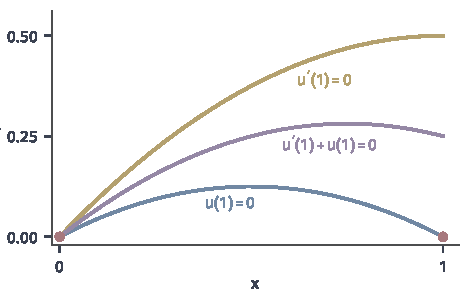
\includegraphics[width=80mm]{figures/06-differential-equations/02-partial-differential-equations/matplotlib/ellip-boundary-types/figure.pdf}
  \caption{同一方程$-u''=1$、同一左端条件$u(0)=0$，右端换三种条件。蓝线$u(1)=0$，解为$x(1-x)/2$；紫线$u'(1)+u(1)=0$，解为$3x/4-x^2/2$；黄线$u'(1)=0$，解为$x-x^2/2$。红点标出取定的边界值。}
  \label{fig:ellip-boundary-types}
\end{BookInlineFigure}

这三个解都可以手算验证。三者都有$-u''=1$和$u(0)=0$，因而都形如$u=Bx-x^2/2$，右端的条件只决定常数$B$：$u(1)=0$给出$B=1/2$，$u'(1)=0$给出$B=1$，$u'(1)+u(1)=0$即$(B-1)+(B-\tfrac12)=0$，给出$B=3/4$。

\paragraph{一致椭圆系数}
后面所有定理都要用到$\bm{A}$的一条性质。在式~\eqref{eq:ellip-divergence-form}两边乘以$u$并积分，会出现二次量$\int\nabla u^\top\bm{A}\nabla u$，它衡量的是梯度带来的能量。我们要求这个量能够控制梯度本身的大小，并且系数不能大到无界。

\begin{definition}[一致椭圆]
\label{def:ellip-uniform}
设$\bm{A}:\Omega\to\mathbb{R}^{d\times d}$可测。若存在常数$0<\kappa_{\min}\leq\kappa_{\max}<\infty$，使几乎所有$\bm{x}\in\Omega$和所有$\bm{\xi}\in\mathbb{R}^{d}$满足
\begin{equation}
 \bm{\xi}^\top\bm{A}(\bm{x})\bm{\xi}\geq\kappa_{\min}\lVert\bm{\xi}\rVert_2^2,\qquad
 \lVert\bm{A}(\bm{x})\bm{\xi}\rVert_2\leq\kappa_{\max}\lVert\bm{\xi}\rVert_2,
 \label{eq:ellip-uniform}
\end{equation}
就称$\bm{A}$在$\Omega$上\term{一致椭圆}（uniformly elliptic）。
\end{definition}

定义不要求$\bm{A}$连续，也不要求对称。系数可以在两种材料的交界处跳变，这在应用中很常见。若$\bm{A}$对称，第一个条件说$\bm{A}(\bm{x})$的最小特征值不小于$\kappa_{\min}$，第二个条件说最大特征值不超过$\kappa_{\max}$。

对任意足够光滑的$u$，取$\bm{\xi}=\nabla u(\bm{x})$，再对$\bm{x}$积分，得到
\begin{equation}
 \int_\Omega\nabla u^\top\bm{A}\nabla u\,\mathrm{d}\bm{x}\geq\kappa_{\min}\int_\Omega\lVert\nabla u\rVert_2^2\,\mathrm{d}\bm{x}.
 \label{eq:ellip-gradient-control}
\end{equation}
这就是一致椭圆的用途：无论梯度指向哪个方向，都有不低于$\kappa_{\min}$的“导热能力”把它计入能量。

图~\ref{fig:ellip-ellipticity}用集合$\{\bm{\xi}:\bm{\xi}^\top\bm{A}\bm{\xi}=1\}$的形状区分三种情况。(a)中$\bm{A}$的元素是$2,0.6,0.6,1$，特征值约为$2.28$和$0.72$，水平集是夹在两个圆之间的椭圆，这是椭圆一词的来历。

(b)中$\bm{A}=\operatorname{diag}(1,0)$，$\xi_2$方向的梯度完全不被计入，能量控制不住这个方向，方程在$x_2$方向没有扩散，这是退化情形。(c)中$\bm{A}=\operatorname{diag}(1,-1)$不定，水平集是双曲线，二次量可以取负，这是波动方程的结构，第~\ref{chap:wave-equations}章要用完全不同的方法处理。

\begin{BookInlineFigure}
  \centering
  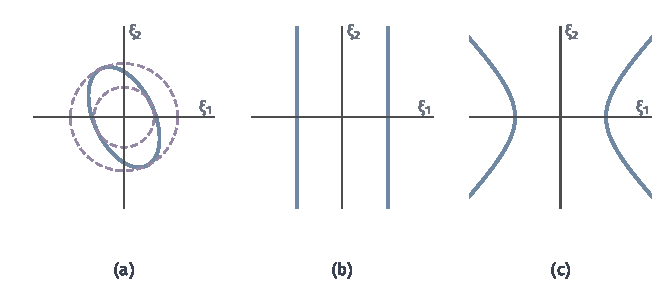
\includegraphics[width=112mm]{figures/06-differential-equations/02-partial-differential-equations/matplotlib/ellip-ellipticity/figure.pdf}
  \caption{水平集$\bm{\xi}^\top\bm{A}\bm{\xi}=1$（蓝线）的三种形状。(a)一致椭圆：椭圆被夹在半径$\kappa_{\max}^{-1/2}$与$\kappa_{\min}^{-1/2}$的两个圆（紫色虚线）之间。(b)退化：$\bm{A}=\operatorname{diag}(1,0)$，水平集是两条平行线，$\xi_2$方向无界。(c)不定：$\bm{A}=\operatorname{diag}(1,-1)$，水平集是双曲线。}
  \label{fig:ellip-ellipticity}
\end{BookInlineFigure}

要注意，主部一致椭圆只说明最高阶项的结构。方程$-\Delta u-k^2u=f$的二阶项与Poisson方程相同，零阶项的符号却相反，它在某些$k$上会失去唯一性，后面的结论不能照搬。本章的主线是式~\eqref{eq:ellip-divergence-form}，低阶项在用到时单独说明条件。


\section{解的表示}
\label{sec:ellip-representation}

能把解写成公式的情形不多，但它们最能说明解由什么决定。下面三种表示各借助一种结构：区间上可以直接积分，线性性允许把点源的响应叠加起来，自伴性允许沿特征函数分解。每个公式都有成立的前提，这些前提与公式一起说明。

\subsection{区间上的求解}
\label{sec:ellip-interval}

先看最简单的两点边值问题。给定$f\in C[0,1]$与边界值$g_0,g_1$，求$u\in C^2[0,1]$满足
\begin{equation}
 -u''=f\quad\text{于}\ (0,1),\qquad u(0)=g_0,\quad u(1)=g_1.
 \label{eq:ellip-interval-dirichlet}
\end{equation}

积分一次，$u'(0)$是一个待定常数，记为$C_1$：
\[
 u'(x)=C_1-\int_0^xf(s)\,\mathrm{d}s .
\]
再积分一次，把二重积分交换次序化成单重积分，$u(0)$是第二个常数：
\[
 u(x)=u(0)+C_1x-\int_0^x(x-s)f(s)\,\mathrm{d}s .
\]

代入左端条件，得到$u(0)=g_0$。代入右端条件，解出$C_1$：
\[
 C_1=g_1-g_0+\int_0^1(1-s)f(s)\,\mathrm{d}s .
\]

两个积分常数恰好被两个边界条件确定。代回去整理，解分成两部分：
\begin{equation}
 u(x)=\underbrace{g_0(1-x)+g_1x}_{\text{边界贡献}}
 +\underbrace{x\int_0^1(1-s)f(s)\,\mathrm{d}s-\int_0^x(x-s)f(s)\,\mathrm{d}s}_{\text{源项贡献}} .
 \label{eq:ellip-interval-solution}
\end{equation}

边界贡献是连接两个边界值的直线，满足$u''=0$。源项贡献在两端为零。这一分解来自线性：边界数据和源项可以分别处理，再把结果相加。

取$f=1$、$g_0=1$、$g_1=3$做一次手算。式~\eqref{eq:ellip-interval-solution}中的积分是
\[
 \int_0^1(1-s)\,\mathrm{d}s=\frac12,\qquad \int_0^x(x-s)\,\mathrm{d}s=\frac{x^2}2 .
\]
于是
\[
 u(x)=(1+2x)+\frac{x}{2}-\frac{x^2}{2}=1+2x+\frac{x(1-x)}{2},
\]
边界贡献是$1+2x$，源项贡献正是式~\eqref{eq:ellip-running-solution}。

唯一性也可以直接读出。若$u_1,u_2$都是解，差$w=u_1-u_2$满足$w''=0$和$w(0)=w(1)=0$。$w''=0$说明$w$是一次函数，两端为零的一次函数只能恒为零。

\paragraph{Neumann条件：相容性与不唯一}
把两端的条件都换成通量。按上一节的约定，外法向在$x=0$处指向左，在$x=1$处指向右，所以问题是
\begin{equation}
 -u''=f\quad\text{于}\ (0,1),\qquad -u'(0)=g_0,\quad u'(1)=g_1.
 \label{eq:ellip-interval-neumann}
\end{equation}
仍然积分一次，这次两端的条件都落在$u'$上，$u$本身一次也没有被约束。

对方程在$[0,1]$上积分，由牛顿--莱布尼茨公式，
\[
 \int_0^1f\,\mathrm{d}x=-u'(1)+u'(0)=-g_1-g_0 .
\]
也就是说，解若存在，数据必须满足
\begin{equation}
 \int_0^1f\,\mathrm{d}x+g_0+g_1=0.
 \label{eq:ellip-interval-compat}
\end{equation}

物理上这是总热量的收支：棒内总产热加上从两端流入的热量必须为零，否则温度不可能稳定。这样的条件称为\term{相容条件}（compatibility condition）。反过来，式~\eqref{eq:ellip-interval-compat}成立时，由$u'(x)=-g_0-\int_0^xf$定义的函数在$x=1$处恰好满足第二个条件，再积分一次就得到解，积分常数$c$可以任取。

取$f(x)=1-2x$，$g_0=g_1=0$。此时$\int_0^1f=0$，相容条件成立。积分得到
\[
 u'(x)=x^2-x,\qquad u(x)=\frac{x^3}{3}-\frac{x^2}{2}+c .
\]
图~\ref{fig:ellip-neumann-compat}(a)是不同$c$对应的解。整条曲线可以上下平移，因为方程和边界条件都只看导数。若要挑出一个代表，可以要求$\int_0^1u=0$，由$\int_0^1(x^3/3-x^2/2)\,\mathrm{d}x=-1/12$得到$c=1/12$。

\begin{BookInlineFigure}
  \centering
  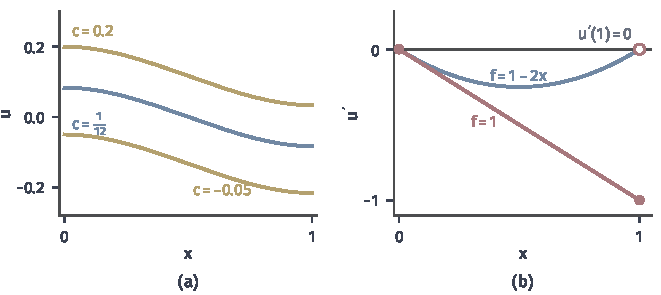
\includegraphics[width=112mm]{figures/06-differential-equations/02-partial-differential-equations/matplotlib/ellip-neumann-compat/figure.pdf}
  \caption{区间上的Neumann问题，$g_0=g_1=0$。(a)$f=1-2x$满足相容条件，解$x^3/3-x^2/2+c$可以任意平移；蓝线是零均值的代表，黄线是另外两个常数。(b)$u'$从$u'(0)=0$（红点）出发：$f=1-2x$时蓝线回到$u'(1)=0$（空心点）；$f=1$时红线走到$-1$，右端条件无法满足。}
  \label{fig:ellip-neumann-compat}
\end{BookInlineFigure}

若取$f=1$，图~\ref{fig:ellip-neumann-compat}(b)显示了失败的方式。从$u'(0)=0$出发，$u'(x)=-x$到右端变成$-1$，而边界要求$0$。两端绝热，棒内持续发热，温度只会不断上升，稳态根本不存在。

对比两种边界条件：Dirichlet问题对任何$f$都唯一可解，Neumann问题只在数据满足一个线性约束时可解，可解时解有一维的自由度。这与线性方程组$\bm{K}\bm{c}=\bm{b}$在$\bm{K}$奇异时的情形相同，后面会把这个对应写清楚。

\subsection{Green函数}
\label{sec:ellip-green}

式~\eqref{eq:ellip-interval-solution}中源项的贡献是对$f$的积分，说明解线性地依赖于$f$。线性依赖应该能写成“每一处的源乘以一个响应，再叠加”。这个响应是什么？

\paragraph{矩阵的逆给出点源响应}
把函数看成长向量，问题就变成矩阵方程。将$[0,1]$等分为$n+1$段，步长$h=1/(n+1)$，内部格点$x_i=ih$。用二阶差商近似$-u''$，边界值为零，得到$\bm{K}\bm{u}=\bm{f}$，其中
\begin{equation}
 \bm{K}=\frac1{h^2}\begin{pmatrix}2&-1&&\\-1&2&\ddots&\\&\ddots&\ddots&-1\\&&-1&2\end{pmatrix}.
 \label{eq:ellip-discrete-laplacian}
\end{equation}

解是$\bm{u}=\bm{K}^{-1}\bm{f}$，写成分量为$u_i=\sum_j(\bm{K}^{-1})_{i,j}f_j$。$\bm{K}^{-1}$的第$j$列，就是只在第$j$个格点放单位源时的整个解。求逆等于把每个格点上的点源响应都算好。

取$n=3$，$h=1/4$，可以手算：
\[
 \bm{K}=16\begin{pmatrix}2&-1&0\\-1&2&-1\\0&-1&2\end{pmatrix},\qquad
 \bm{K}^{-1}=\frac1{64}\begin{pmatrix}3&2&1\\2&4&2\\1&2&3\end{pmatrix}.
\]
每一列先升后降，顶点在对角元处，折线形如帐篷。矩阵对称，说明$y$处放源在$x$处的响应，等于$x$处放源在$y$处的响应。

\paragraph{区间上的点源}
让格点加密，这些帐篷收敛到什么？连续地提问：在$y\in(0,1)$处放一个单位点源，解$G(\cdot,y)$应当满足什么？点源之外没有源，所以$G(\cdot,y)$在$(0,y)$和$(y,1)$上都满足$u''=0$，都是一次函数。加上两端为零，可设
\[
 G(x,y)=\begin{cases}\alpha x,&0\leq x\leq y,\\ \gamma(1-x),&y\leq x\leq1 .\end{cases}
\]

在$y$处需要两个条件。第一，温度连续，否则温度有跳变，热流无穷大，这就是$\alpha y=\gamma(1-y)$。第二，把$-u''=f$在包含$y$的小区间上积分，右端是单位源的总量$1$，左端是$u'$在左右两侧之差的相反数，所以$u'$在$y$处向下跳$1$，这就是$\alpha+\gamma=1$。

两个方程解出$\alpha=1-y$，$\gamma=y$。于是
\begin{equation}
 G(x,y)=\begin{cases}x(1-y),&0\leq x\leq y,\\ y(1-x),&y\leq x\leq1 .\end{cases}
 \label{eq:ellip-green-1d}
\end{equation}
它称为这个边值问题的\term{Green函数}（Green's function）。第~\ref{chap:linear-differential-systems}章也有一个积分核，把脉冲输入变成后续响应，它在脉冲发生之前为零，体现因果。这里的$G$在点源两侧都不为零，因为边界条件把信息从两个方向都传了过来。

有了点源响应，一般的源就是点源的叠加：
\begin{equation}
 u(x)=\int_0^1G(x,y)f(y)\,\mathrm{d}y .
 \label{eq:ellip-green-1d-rep}
\end{equation}
图~\ref{fig:ellip-inverse-tent}验证了矩阵与函数的对应，$\bm{K}^{-1}$除以$h$后，每列的元素恰好落在$G$上。图~\ref{fig:ellip-tents-superposition}展示叠加：几个点源的帐篷相加，点源越多越接近真解。

\begin{BookInlineFigure}
  \centering
  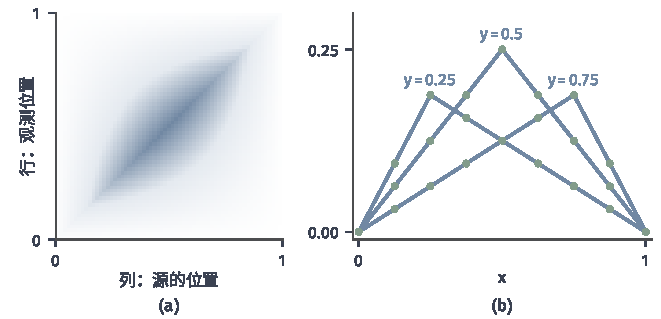
\includegraphics[width=112mm]{figures/06-differential-equations/02-partial-differential-equations/matplotlib/ellip-inverse-tent/figure.pdf}
  \caption{差分矩阵的逆是离散的Green函数。(a)$n=63$时$\bm{K}^{-1}/h$的取值，颜色越深值越大，沿对角线形成山脊。(b)$n=7$时第$2,4,6$列的元素（绿点）与式~\eqref{eq:ellip-green-1d}的$G(\cdot,y)$（蓝线），在格点上数值完全相同。}
  \label{fig:ellip-inverse-tent}
\end{BookInlineFigure}

现在验证式~\eqref{eq:ellip-green-1d-rep}。把积分在$y=x$处拆开，代入式~\eqref{eq:ellip-green-1d}：
\[
 u(x)=(1-x)\int_0^xyf(y)\,\mathrm{d}y+x\int_x^1(1-y)f(y)\,\mathrm{d}y .
\]

对$x$求导，积分限上出现的两项是$(1-x)xf(x)$和$-x(1-x)f(x)$，互相抵消，只剩
\[
 u'(x)=-\int_0^xyf(y)\,\mathrm{d}y+\int_x^1(1-y)f(y)\,\mathrm{d}y .
\]

再求导，得到
\[
 u''(x)=-xf(x)-(1-x)f(x)=-f(x).
\]
又由公式直接读出$u(0)=u(1)=0$。取$f=1$，
\[
 u(x)=(1-x)\frac{x^2}{2}+x\frac{(1-x)^2}{2}=\frac{x(1-x)}{2},
\]
这正是式~\eqref{eq:ellip-running-solution}。

\begin{BookInlineFigure}
  \centering
  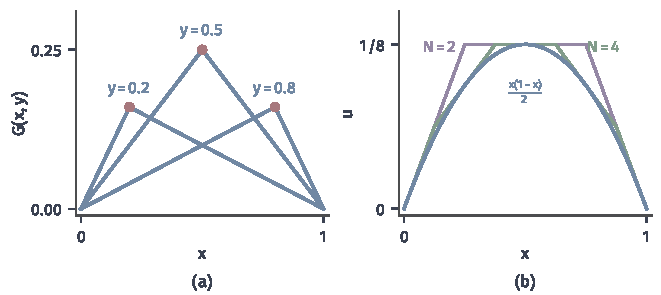
\includegraphics[width=112mm]{figures/06-differential-equations/02-partial-differential-equations/matplotlib/ellip-tents-superposition/figure.pdf}
  \caption{点源响应的叠加。(a)三个位置$y$处的单位点源产生的帐篷$G(\cdot,y)$，红点是顶点$(y,y(1-y))$。(b)均匀源$f=1$的离散近似：在$N$个等分小段的中点放权重$1/N$的点源，紫线$N=2$，绿线$N=4$，$N$增大时趋于蓝线$x(1-x)/2$。}
  \label{fig:ellip-tents-superposition}
\end{BookInlineFigure}

\paragraph{全空间的基本解}
多维情形不能分段积分，但点源响应的想法仍然有效。先在没有边界的全空间里问：单位点源在原点产生的平衡温度是什么？

对称性告诉我们解只依赖于到原点的距离$r=\lVert\bm{x}\rVert_2$，记为$\varphi(r)$。把所有热量想成从原点向外流：稳态下，单位热源产生的热量必须全部穿过每一个以原点为心的球面。半径$r$的球面面积是$d\omega_dr^{d-1}$，其中$\omega_d$是单位球的体积。所以径向热流密度为
\[
 -\varphi'(r)=\frac1{d\omega_dr^{d-1}} .
\]

积分一次，常数取最简单的值，就得到\termalias{基本解-偏微分方程}{基本解}（fundamental solution）
\begin{equation}
 \Phi(\bm{x})=\begin{cases}
 -\dfrac{\lVert\bm{x}\rVert_2}{2},&d=1,\\
 -\dfrac1{2\pi}\log\lVert\bm{x}\rVert_2,&d=2,\\
 \dfrac1{d(d-2)\omega_d}\,\lVert\bm{x}\rVert_2^{2-d},&d\geq3 .
 \end{cases}
 \label{eq:ellip-fundamental}
\end{equation}
$d=3$时$\omega_3=4\pi/3$，$\Phi=1/(4\pi\lVert\bm{x}\rVert_2)$。直接计算可知$\Delta\Phi=0$在原点之外成立：径向函数的Laplace是$r^{1-d}(r^{d-1}\varphi')'$，而$r^{d-1}\varphi'$是常数。

图~\ref{fig:ellip-fundamental-radial}比较了三个维数。维数越高，球面面积随半径增长越快，同样的热量摊得越薄，所以(b)中的流密度衰减得越快。$d=1$时热流不衰减，$\Phi$一直线性下降；$d\geq3$时$\Phi$在无穷远趋于零；$d=2$介于两者之间，$\Phi$对数发散。

\begin{BookInlineFigure}
  \centering
  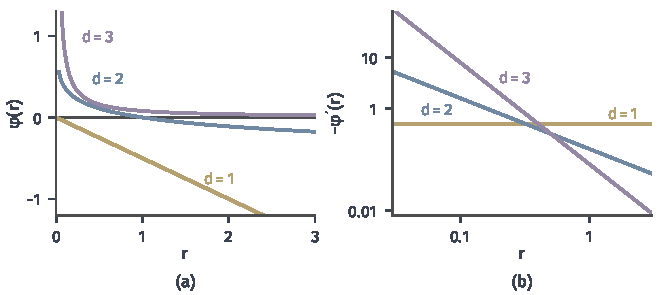
\includegraphics[width=112mm]{figures/06-differential-equations/02-partial-differential-equations/matplotlib/ellip-fundamental-radial/figure.pdf}
  \caption{基本解的径向形状。(a)$\varphi(r)$：$d=1$（黄）是直线，$d=2$（蓝）是对数，$d=3$（紫）是$1/(4\pi r)$，$d\geq2$时在原点发散。(b)流密度$-\varphi'(r)$的双对数图，斜率分别为$0,-1,-2$，体现单位热量摊在面积$d\omega_dr^{d-1}$上。}
  \label{fig:ellip-fundamental-radial}
\end{BookInlineFigure}

基本解只回答了全空间的问题。对紧支撑的$C^2$函数$f$，卷积
\[
 v(\bm{x})=\int_{\mathbb{R}^{d}}\Phi(\bm{x}-\bm{y})f(\bm{y})\,\mathrm{d}\bm{y}
\]
满足$-\Delta v=f$，这在下面的表示定理之后就能验证。但$v$不满足任何给定的边界条件。在$(0,1)$上取$f=1$，
\[
 v(x)=-\int_0^1\frac{\lvert x-y\rvert}{2}\,\mathrm{d}y=-\frac{x^2+(1-x)^2}{4},
\]
边界值$v(0)=v(1)=-1/4$不是$0$。它比真解$x(1-x)/2$处处低$1/4$，必须修正。

\paragraph{表示公式}
要知道边界怎样影响解，用Green第二恒等式。设$V$是有界区域，$\partial V$足够光滑，$u,w\in C^2(\overline V)$。向量场$u\nabla w-w\nabla u$的散度是
\[
 \nabla\cdot(u\nabla w-w\nabla u)=u\Delta w-w\Delta u .
\]
对它用散度定理，得到
\begin{equation}
 \int_V(u\Delta w-w\Delta u)\,\mathrm{d}\bm{x}=\int_{\partial V}(u\,\partial_{\bm{n}}w-w\,\partial_{\bm{n}}u)\,\mathrm{d}S,
 \label{eq:ellip-green-second}
\end{equation}
其中$\partial_{\bm{n}}w=\bm{n}\cdot\nabla w$是外法向导数。

我们想取$w=\Phi(\bm{x}-\cdot)$，但它在$\bm{x}$处奇异。办法是挖掉以$\bm{x}$为中心的小球，见图~\ref{fig:ellip-excised-ball}，在剩下的区域用恒等式，再让球缩小。

\begin{BookInlineFigure}
  \centering
  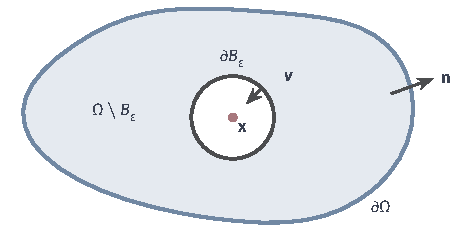
\includegraphics[width=78mm]{figures/06-differential-equations/02-partial-differential-equations/tikz/ellip-excised-ball/figure.pdf}
  \caption{挖去小球后的区域$\Omega\setminus B_\varepsilon$。外边界上的法向$\bm{n}$指向区域外，小球面上区域的外法向$\bm{\nu}$指向球心$\bm{x}$。}
  \label{fig:ellip-excised-ball}
\end{BookInlineFigure}

\begin{theorem}[Green表示公式]
\label{thm:ellip-representation}
设$d\geq2$，$\Omega\subset\mathbb{R}^{d}$是边界光滑的有界区域，$u\in C^2(\overline\Omega)$。则对每个$\bm{x}\in\Omega$，
\begin{equation}
 \begin{aligned}
 u(\bm{x})={}&\int_\Omega\Phi(\bm{x}-\bm{y})\bigl(-\Delta u(\bm{y})\bigr)\,\mathrm{d}\bm{y}\\
 &+\int_{\partial\Omega}\Bigl(\Phi(\bm{x}-\bm{y})\,\partial_{\bm{n}}u(\bm{y})-u(\bm{y})\,\partial_{\bm{n}}\Phi(\bm{x}-\bm{y})\Bigr)\,\mathrm{d}S(\bm{y}),
 \end{aligned}
 \label{eq:ellip-representation}
\end{equation}
其中法向导数对变量$\bm{y}$求。
\end{theorem}

\begin{proof}
固定$\bm{x}$，记$w(\bm{y})=\Phi(\bm{x}-\bm{y})$，取$\varepsilon$足够小使$\overline{B_\varepsilon(\bm{x})}\subset\Omega$，令$V=\Omega\setminus\overline{B_\varepsilon(\bm{x})}$。在$V$上$\Delta w=0$，式~\eqref{eq:ellip-green-second}化为
\[
 -\int_Vw\Delta u\,\mathrm{d}\bm{y}=\int_{\partial\Omega}(u\,\partial_{\bm{n}}w-w\,\partial_{\bm{n}}u)\,\mathrm{d}S+\int_{\partial B_\varepsilon}(u\,\partial_{\bm{\nu}}w-w\,\partial_{\bm{\nu}}u)\,\mathrm{d}S .
\]

在小球面上，$\bm{\nu}$指向球心，$w$的值是$\varphi(\varepsilon)$，方向导数是
\[
 \partial_{\bm{\nu}}w=-\varphi'(\varepsilon)=\frac1{d\omega_d\varepsilon^{d-1}},
\]
它正好是球面面积的倒数。于是第一项是$u$在球面上的平均值：
\[
 \int_{\partial B_\varepsilon}u\,\partial_{\bm{\nu}}w\,\mathrm{d}S=\frac1{\lvert\partial B_\varepsilon\rvert}\int_{\partial B_\varepsilon}u\,\mathrm{d}S\ \longrightarrow\ u(\bm{x}),\qquad\varepsilon\to0,
\]
极限成立是因为$u$连续。

第二项的绝对值不超过$\lvert\varphi(\varepsilon)\rvert\cdot d\omega_d\varepsilon^{d-1}\cdot\max\lVert\nabla u\rVert_2$。$d=2$时这是$\varepsilon\lvert\log\varepsilon\rvert$的倍数，$d\geq3$时是$\varepsilon$的倍数，都趋于零。

最后，$\Phi(\bm{x}-\cdot)$在$\bm{x}$附近可积，$\Delta u$有界，左端的积分当$\varepsilon\to0$时收敛到$\int_\Omega w\Delta u$的相反数。三个极限合起来，移项即得式~\eqref{eq:ellip-representation}。
\end{proof}

现在可以补上卷积的验证。设$f\in C_c^2(\mathbb{R}^{d})$，把导数放到$f$上，有$\Delta v=\Phi*\Delta f$。把定理用于$u=f$、足够大的球$\Omega$，边界项为零，给出$f=\Phi*(-\Delta f)$，所以$-\Delta v=f$。

式~\eqref{eq:ellip-representation}还不能算是解的公式，因为右端同时用到了边界上的$u$和$\partial_{\bm{n}}u$。对Dirichlet问题，$\partial_{\bm{n}}u$恰恰是未知的。要把它消掉。

\paragraph{区域的Green函数}
办法是给基本解加一个调和的修正，使修正后的函数在边界上为零，这样含$\partial_{\bm{n}}u$的项就消失了。

\begin{definition}[区域的Green函数]
\label{def:ellip-green-domain}
设$\Omega$是有界区域。若对每个$\bm{x}\in\Omega$，存在$h^{\bm{x}}\in C^2(\overline\Omega)$满足$\Delta h^{\bm{x}}=0$，且在$\partial\Omega$上$h^{\bm{x}}(\bm{y})=\Phi(\bm{x}-\bm{y})$，则称
\begin{equation}
 G(\bm{x},\bm{y})=\Phi(\bm{x}-\bm{y})-h^{\bm{x}}(\bm{y})
 \label{eq:ellip-green-domain}
\end{equation}
为$\Omega$上Dirichlet问题的Green函数。
\end{definition}

$\Phi$负责在点源处产生正确的奇性，$h^{\bm{x}}$负责抵消边界值。图~\ref{fig:ellip-green-corrector}在一维展示了这个构造：黄色的基本解在两端不为零，紫色的修正是过这两个端点值的直线，两者相减就是蓝色的帐篷。$\Phi$在全空间只有一个，而$G$随着区域变化，换一个区域就要重新解一次修正问题。

\begin{BookInlineFigure}
  \centering
  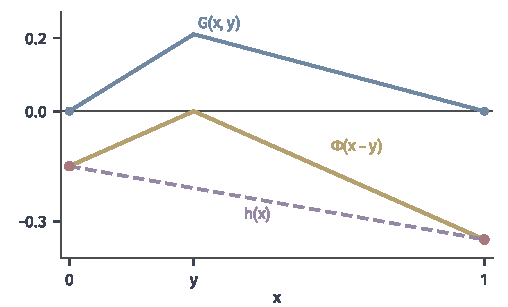
\includegraphics[width=86mm]{figures/06-differential-equations/02-partial-differential-equations/matplotlib/ellip-green-corrector/figure.pdf}
  \caption{一维Green函数的构造，$y=0.3$。黄线是基本解$\Phi(x-y)=-\lvert x-y\rvert/2$，红点是它的两个端点值。紫色虚线$h$是以这两个值为端点的直线，$h''=0$。蓝线$G=\Phi-h$在两端为零，就是式~\eqref{eq:ellip-green-1d}。}
  \label{fig:ellip-green-corrector}
\end{BookInlineFigure}

用$u$和$h^{\bm{x}}$再做一次式~\eqref{eq:ellip-green-second}，由$\Delta h^{\bm{x}}=0$得到
\[
 \int_\Omega h^{\bm{x}}\bigl(-\Delta u\bigr)\,\mathrm{d}\bm{y}=\int_{\partial\Omega}\bigl(u\,\partial_{\bm{n}}h^{\bm{x}}-h^{\bm{x}}\,\partial_{\bm{n}}u\bigr)\,\mathrm{d}S .
\]

用式~\eqref{eq:ellip-representation}减去这个等式。在边界上$\Phi=h^{\bm{x}}$，含$\partial_{\bm{n}}u$的两项抵消，得到
\begin{equation}
 u(\bm{x})=\int_\Omega G(\bm{x},\bm{y})\bigl(-\Delta u(\bm{y})\bigr)\,\mathrm{d}\bm{y}-\int_{\partial\Omega}u(\bm{y})\,\partial_{\bm{n}}G(\bm{x},\bm{y})\,\mathrm{d}S(\bm{y}) .
 \label{eq:ellip-green-rep}
\end{equation}

这个公式把解分成两份，第一份由源项产生，第二份由边界值产生。边界贡献不能省略，否则非零边值的信息就丢了。一维的验证很直接：端点$y=0$的外法向指向左，$\partial_{\bm{n}}G=-\partial_yG(x,0)=-(1-x)$，边界项给出$g_0(1-x)$；同样$y=1$处给出$g_1x$。两项合起来就是式~\eqref{eq:ellip-interval-solution}中的那条直线。

要小心公式的逻辑方向。式~\eqref{eq:ellip-green-rep}是说：\emph{如果}$C^2(\overline\Omega)$的解存在，\emph{并且}Green函数存在且足够光滑，解就必须是这个样子。它推出了唯一性，但没有证明存在性。

\paragraph{像源法}
几何特别简单时，修正项可以直接猜出来。考虑上半平面$\{x_2>0\}$，点源在$\bm{y}=(y_1,y_2)$。在边界另一侧的镜像点$\bm{y}^{*}=(y_1,-y_2)$放一个负的点源，由对称性，边界$x_2=0$上每一点到$\bm{y}$与到$\bm{y}^{*}$的距离相等，两个势在边界上抵消。这种做法称为\term{像源法}（method of images），二维的Green函数是
\begin{equation}
 G(\bm{x},\bm{y})=-\frac1{2\pi}\bigl(\log\lVert\bm{x}-\bm{y}\rVert_2-\log\lVert\bm{x}-\bm{y}^{*}\rVert_2\bigr).
 \label{eq:ellip-green-half-plane}
\end{equation}

半平面的外法向是$-\bm{e}_2$，把$-\partial_{\bm{n}}G=\partial_{y_2}G$在$y_2=0$处算出来：
\[
 P(\bm{x},y_1)=\frac{x_2}{\pi\bigl((x_1-y_1)^2+x_2^2\bigr)} .
\]
边界数据$g$产生的解是
\[
 u(\bm{x})=\int_{\mathbb{R}}P(\bm{x},y_1)\,g(y_1)\,\mathrm{d}y_1 ,
\]
$P$称为半平面的\term{Poisson核}（Poisson kernel）。半平面无界，这个公式对有界连续的$g$给出有界调和函数，要证明解确实取到边界值，需要对$P$的集中性质单独做极限估计，这里不细述。

图~\ref{fig:ellip-image-method}(b)说明Poisson核是一个加权平均：离边界越近，权重越集中在最近的边界点附近。这与解的边值恰好是$g$相吻合。离边界越远，权重摊得越开，解越光滑。

\begin{BookInlineFigure}
  \centering
  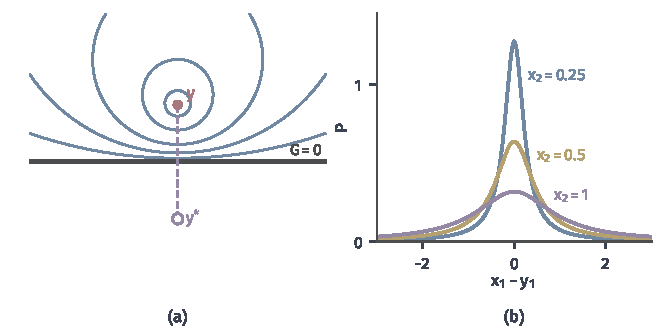
\includegraphics[width=112mm]{figures/06-differential-equations/02-partial-differential-equations/matplotlib/ellip-image-method/figure.pdf}
  \caption{上半平面的Green函数。(a)红点$\bm{y}=(0,1)$是点源，紫色空心点$\bm{y}^{*}=(0,-1)$是虚设的负像源，蓝线是$G$的等值线，粗线是边界，边界上$G=0$。(b)Poisson核$P$随$x_1-y_1$的变化，$x_2$越小峰越尖；每条曲线下的面积都是$1$。}
  \label{fig:ellip-image-method}
\end{BookInlineFigure}

\subsection{谱展开}
\label{sec:ellip-spectral}

Green函数把解写成“一处一处”的叠加。另一种思路是“一个模式一个模式”地叠加：找一组基，使微分算子在这组基下成为对角的，求解就成了逐个系数的除法。这正是对称矩阵的做法。

\paragraph{从矩阵的对角化到函数}
若$\bm{K}$对称正定，$\bm{K}=\bm{Q}\bm{\Lambda}\bm{Q}^\top$，那么$\bm{K}\bm{u}=\bm{f}$的解是把$\bm{f}$在特征向量上分解，每个分量除以对应的特征值，再合成。连续的对应物是
\begin{equation}
 -\Delta e_k=\lambda_ke_k\quad\text{于}\ \Omega,\qquad e_k=0\quad\text{于}\ \partial\Omega .
 \label{eq:ellip-eigenproblem}
\end{equation}

在区间$(0,1)$上，满足这个问题的函数和特征值是
\[
 e_k(x)=\sqrt2\sin(k\pi x),\qquad\lambda_k=k^2\pi^2,\qquad k\geq1 .
\]
这组函数是$L^2(0,1)$的标准正交基，它与Fourier级数的完备性同源，可参考\BookChapterRef{chap:fourier-transform}{卷四第14章“Fourier变换”}。把$f$与$u$按这组基展开，系数记为$f_k=\langle f,e_k\rangle$，$u_k=\langle u,e_k\rangle$。

用$e_k$乘方程$-u''=f$并积分，分部积分两次。$u$和$e_k$在端点都为零，边界项消失，得到
\[
 f_k=\int_0^1(-u'')e_k\,\mathrm{d}x=\int_0^1u(-e_k'')\,\mathrm{d}x=\lambda_ku_k .
\]
于是
\begin{equation}
 u=\sum_{k\geq1}\frac{f_k}{\lambda_k}\,e_k .
 \label{eq:ellip-spectral-solution}
\end{equation}

这个过程用到了边界条件的自伴结构：分部积分时$u$和$e_k$的边界项同时消失，$-\mathrm{d}^2/\mathrm{d}x^2$才能从$u$移到$e_k$上。对一般的有界区域，这样一组基是否存在，要等弱解理论建立之后才能回答。

\paragraph{一个完整的计算}
继续用$f=1$。系数是
\[
 f_k=\sqrt2\int_0^1\sin(k\pi x)\,\mathrm{d}x=\frac{\sqrt2\,(1-(-1)^k)}{k\pi} .
\]
偶数$k$的系数为零，奇数$k$的系数为$2\sqrt2/(k\pi)$。代入式~\eqref{eq:ellip-spectral-solution}，
\[
 u(x)=\sum_{k\ \text{奇}}\frac{4}{k^3\pi^3}\sin(k\pi x).
\]

在中点$x=1/2$处算几项部分和。$\sin(k\pi/2)$对$k=1,3,5$依次是$1,-1,1$，于是
\[
 \frac4{\pi^3}\approx0.12901,\qquad
 \frac4{\pi^3}\Bigl(1-\frac1{27}\Bigr)\approx0.12423,\qquad
 \frac4{\pi^3}\Bigl(1-\frac1{27}+\frac1{125}\Bigr)\approx0.12526 ,
\]
正在收敛到式~\eqref{eq:ellip-running-solution}给出的$1/8=0.125$。

图~\ref{fig:ellip-modes-coeffs}对比了$f$与$u$的系数。$f_k$按$1/k$衰减，所以部分和在间断处有明显的振荡，这是$f$在端点从$1$跳到边界值$0$的结果。$u_k=f_k/\lambda_k$按$1/k^3$衰减，只取第一项就已经和真解很接近。

除以$\lambda_k$压低高频，这就是椭圆问题的光滑作用。解比数据多出两阶导数的正则性，这在系数上表现为多出$k^{-2}$的衰减。

\begin{BookInlineFigure}
  \centering
  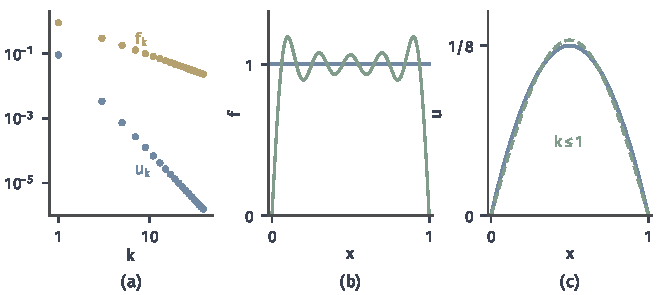
\includegraphics[width=112mm]{figures/06-differential-equations/02-partial-differential-equations/matplotlib/ellip-modes-coeffs/figure.pdf}
  \caption{$f=1$的正弦展开。(a)奇数$k$上$f_k$（黄）与$u_k=f_k/\lambda_k$（蓝）的双对数图，衰减率分别是$k^{-1}$与$k^{-3}$。(b)$f$的$k\leq9$部分和（绿）在$f$的目标值（蓝）附近振荡。(c)$u$的第一项（绿色虚线）已贴近真解（蓝）。}
  \label{fig:ellip-modes-coeffs}
\end{BookInlineFigure}

$f\in L^2(0,1)$时，式~\eqref{eq:ellip-spectral-solution}在$L^2$意义下收敛，它的导数级数也在$L^2$中收敛，这由下面两个有限的和保证：
\[
 \sum_k\frac{f_k^2}{\lambda_k^2}\leq\frac1{\lambda_1^2}\sum_kf_k^2<\infty,\qquad
 \sum_k\lambda_ku_k^2=\sum_k\frac{f_k^2}{\lambda_k}<\infty .
\]
逐点收敛和逐项求二阶导需要$f$有更多的光滑性，不能仅凭$f\in L^2$断言。

把$u_k=f_k/\lambda_k$的定义代回，再交换求和与积分，还能读出Green函数的谱表示：
\begin{equation}
 G(x,y)=\sum_{k\geq1}\frac{e_k(x)\,e_k(y)}{\lambda_k},
 \label{eq:ellip-green-spectral}
\end{equation}
这是矩阵等式$\bm{K}^{-1}=\sum_k\bm{q}_k\bm{q}_k^\top/\lambda_k$的函数版本。两种表示说的是同一个算子，一个按位置分解，一个按频率分解。

\paragraph{矩形区域}
积分区域是矩形时，变量分离给出二维的特征函数。在单位正方形上，
\[
 e_{m,n}(x_1,x_2)=2\sin(m\pi x_1)\sin(n\pi x_2),\qquad \lambda_{m,n}=\pi^2(m^2+n^2).
\]

若$f$恰好是单个模式，如$f=\sin(\pi x_1)\sin(\pi x_2)$，解就是$u=f/(2\pi^2)$，一次除法完成。取$f=1$，系数只在$m,n$都是奇数时非零，计算与一维相同，
\begin{equation}
 \begin{gathered}
 u(x_1,x_2)=\sum_{m,n\ \text{奇}}c_{m,n}\sin(m\pi x_1)\sin(n\pi x_2),\\
 c_{m,n}=\frac{16}{\pi^4mn(m^2+n^2)} .
 \end{gathered}
 \label{eq:ellip-square-series}
\end{equation}
图~\ref{fig:ellip-square-series}显示解的形状和中心点的收敛。第一项给出的中心值是$16/(2\pi^4)\approx0.0821$，加入更多项后趋于约$0.0737$。

\begin{BookInlineFigure}
  \centering
  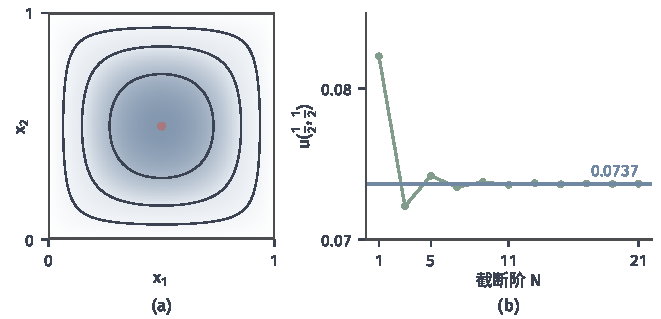
\includegraphics[width=112mm]{figures/06-differential-equations/02-partial-differential-equations/matplotlib/ellip-square-series/figure.pdf}
  \caption{单位正方形上$-\Delta u=1$、零Dirichlet边界的解。(a)$u$的取值，颜色越深值越大，等值线取$0.02,0.04,0.06$；角点附近的等值线被挤成圆角，红点是中心。(b)式~\eqref{eq:ellip-square-series}取$m,n\leq N$的中心值（绿）趋于蓝线。}
  \label{fig:ellip-square-series}
\end{BookInlineFigure}

\paragraph{零特征值}
把边界条件换成Neumann条件，特征问题的解变成$e_0=1$和$e_k=\sqrt2\cos(k\pi x)$，$\lambda_0=0$，$\lambda_k=k^2\pi^2$。式~\eqref{eq:ellip-spectral-solution}的第$k=0$项要除以$0$，不能直接用。

回到$\lambda_ku_k=f_k$这个关系，它对$k=0$说的是
\[
 0\cdot u_0=f_0=\int_0^1f\,\mathrm{d}x .
\]
这个等式有解当且仅当$f_0=0$，即相容条件~\eqref{eq:ellip-interval-compat}（$g_0=g_1=0$时）；一旦成立，$u_0$可以任取，这正是相差常数的不唯一。所以要先检查核空间上的分量，再对非零特征值做除法。

以$f=1-2x$为例，$f_0=0$，其余系数由分部积分算出，奇数$k$时$f_k=4\sqrt2/(k\pi)^2$，偶数$k$（$k\geq2$）时$f_k=0$。于是零均值的解是
\[
 u(x)=\sum_{k\ \text{奇}}\frac{8}{k^4\pi^4}\cos(k\pi x).
\]
在$x=0$处，第一项是$8/\pi^4\approx0.0821$，加上$k=3$的一项后约为$0.0831$，与前面的精确值$u(0)=1/12\approx0.0833$一致。


\section{弱形式}
\label{sec:ellip-weak}

前面的公式都假设解有连续的二阶导数。这个假设常常不成立。考虑一根由两种材料接成的棒：$a=1$于$(0,1/2)$，$a=4$于$(1/2,1)$，源项$f=1$，两端温度为零。系数在中点跳变，方程~\eqref{eq:ellip-1d-equation}中的$(au')'$在中点该怎么理解？

\paragraph{一个没有经典解的问题}
先按物理来算。热流$q=-au'$满足$q'=1$，所以$q(x)=x+C$在整段上是一条直线；热流穿过界面时不会凭空消失，因而$q$连续。由此得到$u'=-(x+C)/a$，它在中点有跳跃。

再用$u(0)=u(1)=0$定常数。温度沿整段的变化为零：
\[
 0=\int_0^1u'\,\mathrm{d}x=-\int_0^{1/2}(x+C)\,\mathrm{d}x-\frac14\int_{1/2}^1(x+C)\,\mathrm{d}x .
\]

算出两个积分并代入，得到
\[
 -\Bigl(\frac18+\frac C2\Bigr)-\frac14\Bigl(\frac38+\frac C2\Bigr)=-\frac7{32}-\frac{5C}8=0,
\]
所以$C=-7/20$。中点的温度是$u(1/2)=-(1/8+C/2)=1/20=0.05$。

图~\ref{fig:ellip-coefficient-jump}是这个解。$u$连续而在中点有折角，$u'$从$-0.15$跳到$-0.0375$，所以$u$不是$C^2$函数，甚至不是$C^1$函数，在中点逐点谈论方程是没有意义的。可是物理上这个解完全合理，热流$q$也是连续的。我们需要一种能接纳它的“解”的定义。

\begin{BookInlineFigure}
  \centering
  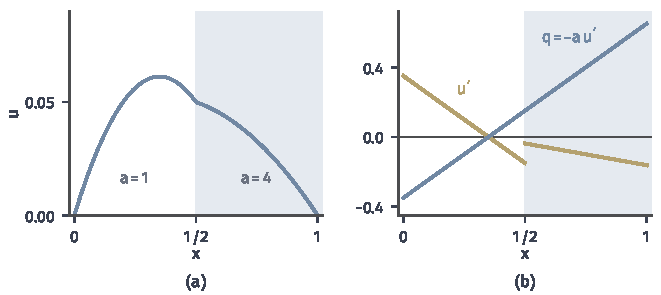
\includegraphics[width=112mm]{figures/06-differential-equations/02-partial-differential-equations/matplotlib/ellip-coefficient-jump/figure.pdf}
  \caption{两段材料接成的棒，$f=1$，两端温度为零，右半段（浅蓝底）导热率为$4$。(a)温度$u$连续，在中点有折角。(b)$u'$（黄）在中点跳跃，热流$q=-au'$（蓝）是一条连续的直线。}
  \label{fig:ellip-coefficient-jump}
\end{BookInlineFigure}

\paragraph{用测试函数检验}
经典解要求方程在每一点成立。换一种检验方式：取光滑的“探针”函数$v$，它只在某一小块区域内不为零，读取方程两边在这块区域上的加权平均。若对所有探针读数都相等，就说方程成立。这样的$v$称为\term{测试函数}（test function）。

用式~\eqref{eq:ellip-1d-equation}检验：两边乘以在两端为零的$v$，积分，并分部积分一次，把一个导数从$au'$移到$v$上：
\[
 \int_0^1fv\,\mathrm{d}x=-\int_0^1(au')'v\,\mathrm{d}x=\int_0^1au'v'\,\mathrm{d}x-\bigl[au'v\bigr]_0^1 .
\]
$v$在两端为零，边界项消失，于是
\begin{equation}
 \int_0^1a\,u'v'\,\mathrm{d}x=\int_0^1fv\,\mathrm{d}x .
 \label{eq:ellip-weak-1d}
\end{equation}

式~\eqref{eq:ellip-weak-1d}只含$u$的一阶导数，$a$也不需要可导。上面的折线型解可以直接代入。取$v=x(1-x)$，$v'=1-2x$，由$au'=-(x+C)$，两段合起来得到
\[
 \int_0^1au'v'\,\mathrm{d}x=-\int_0^1\Bigl(x-\frac7{20}\Bigr)(1-2x)\,\mathrm{d}x=\frac16,
\]
右端$\int_0^1fv\,\mathrm{d}x$也是$\int_0^1x(1-x)\,\mathrm{d}x=1/6$，两边相等。界面处的通量连续性不用单独写，它已经包含在弱形式中。

\begin{BookInlineFigure}
  \centering
  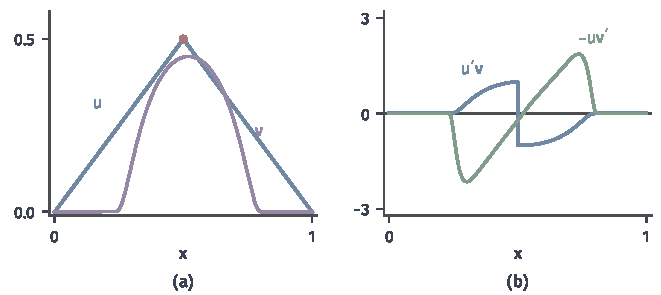
\includegraphics[width=112mm]{figures/06-differential-equations/02-partial-differential-equations/matplotlib/ellip-test-probe/figure.pdf}
  \caption{把导数转移到测试函数上。(a)$u=\tfrac12-\lvert x-\tfrac12\rvert$在红点处有折角，紫线是支撑在$(0.22,0.82)$内的光滑测试函数$v$（画为$0.45$倍）。(b)蓝线$u'v$在折角处跳跃，绿线$-uv'$连续。两条曲线不同，下方的积分却相同，数值积分都约为$-0.040$。}
  \label{fig:ellip-test-probe}
\end{BookInlineFigure}

这个动作的实质是让测试函数承担一半的导数，如图~\ref{fig:ellip-test-probe}所示。卷四用同样的动作定义了弱导数，这里只是把它用于方程。下面把多维的对应写出来，$\bm{A}$的条件沿用定义~\ref{def:ellip-uniform}。

\paragraph{多维的分部积分}
设$\Omega$是有界Lipschitz区域，$u,v$足够光滑。向量场$v\,\bm{A}\nabla u$的散度由乘积法则给出：
\[
 \nabla\cdot(v\bm{A}\nabla u)=\nabla v\cdot\bm{A}\nabla u+v\,\nabla\cdot(\bm{A}\nabla u) .
\]
对它用散度定理，得到
\begin{equation}
 \int_\Omega\bigl(-\nabla\cdot(\bm{A}\nabla u)\bigr)v\,\mathrm{d}\bm{x}
 =\int_\Omega\bm{A}\nabla u\cdot\nabla v\,\mathrm{d}\bm{x}-\int_{\partial\Omega}(\bm{n}\cdot\bm{A}\nabla u)\,v\,\mathrm{d}S .
 \label{eq:ellip-green-first}
\end{equation}
这是Green第一恒等式的一般形式。左端要两阶导数，右端的体积分只要一阶，边界项显示了边界通量在哪里出现。

由此定义贯穿全章的\term{双线性型}（bilinear form）
\begin{equation}
 a(u,v)=\int_\Omega\bm{A}\nabla u\cdot\nabla v\,\mathrm{d}\bm{x}.
 \label{eq:ellip-bilinear}
\end{equation}

\paragraph{用到的空间}
式~\eqref{eq:ellip-bilinear}有意义，只需要$u,v$有平方可积的一阶弱导数，这就是Sobolev空间$H^1(\Omega)$。回忆几个事实，其详细讨论可参考\BookChapterRef{chap:sobolev-spaces}{卷四第21章“Sobolev空间”}：

\begin{itemize}
 \item $H^1(\Omega)$由$L^2(\Omega)$中弱梯度也在$L^2$中的函数组成，按函数值和梯度的$L^2$内积之和定义内积后，它是Hilbert空间；
 \item 在有界Lipschitz区域上，存在把$H^1(\Omega)$映到$L^2(\partial\Omega)$的有界线性迹算子$\operatorname{Tr}$，对光滑到边界的函数就是限制到边界；
 \item $H^1_0(\Omega)$是$C_c^\infty(\Omega)$在$H^1$范数下的闭包，有界Lipschitz区域上它恰好是迹为零的函数组成的闭子空间。
\end{itemize}

本章记$\lVert v\rVert_2$为$L^2(\Omega)$范数，$\lVert\nabla v\rVert_2$为$\lVert\nabla v(\bm{x})\rVert_2$的$L^2(\Omega)$范数，$H^1$范数则由下式给出：
\[
 \lVert v\rVert_{H^1}^2=\lVert v\rVert_2^2+\lVert\nabla v\rVert_2^2 .
\]

函数值在边界上的约束要借助迹来表达，因为$H^1$函数只是几乎处处定义的等价类，边界是零测集，不能读取一个代表的边界值。右端的$\int_\Omega fv$只要求$f\in L^2(\Omega)$，甚至可以更弱：只要$v\mapsto\ell(v)$是$H^1_0(\Omega)$上的有界线性泛函。这样的泛函全体记为$H^{-1}(\Omega)$。

下面按边界条件的类型分别写出弱形式。两类条件的处理方式完全不同：一类写进函数空间，一类写进积分。

\subsection{Dirichlet条件}
\label{sec:ellip-weak-dirichlet}

对问题$-\nabla\cdot(\bm{A}\nabla u)=f$，$u=g$于$\partial\Omega$，式~\eqref{eq:ellip-green-first}中含未知的边界通量。测试函数取零迹时，这一项直接消失，所以测试函数应取在$H^1_0(\Omega)$中。

解要满足边界值$g$，这是对$u$的约束，写成$\operatorname{Tr}u=g$。要让这个条件有意义，$g$必须是某个$H^1(\Omega)$函数的迹，满足这个要求的边界函数组成迹空间，通常记为$H^{1/2}(\partial\Omega)$。于是有下面的定义。

\begin{definition}[Dirichlet问题的弱解]
\label{def:ellip-weak-dirichlet}
设$\Omega$是有界Lipschitz区域，$\bm{A}$一致椭圆，$f\in L^2(\Omega)$，$g=\operatorname{Tr}R$，其中$R\in H^1(\Omega)$。若$u\in H^1(\Omega)$满足$\operatorname{Tr}u=g$，且
\begin{equation}
 a(u,v)=\int_\Omega fv\,\mathrm{d}\bm{x}\qquad\text{对所有}\ v\in H^1_0(\Omega),
 \label{eq:ellip-weak-dirichlet}
\end{equation}
就称$u$是该问题的\term{弱解}（weak solution）。式~\eqref{eq:ellip-weak-dirichlet}称为\term{弱形式}（weak formulation）。
\end{definition}

这里要分清两组函数。候选的解称为试探函数，它们组成的集合是$\{u\in H^1(\Omega):\operatorname{Tr}u=g\}$，$g\neq0$时这不是线性空间，两个解之和的迹是$2g$。测试函数在$H^1_0(\Omega)$中，它是线性空间。

\paragraph{边界提升}
两者的关系是：试探函数的集合是$H^1_0(\Omega)$的一个平移。取任一满足$\operatorname{Tr}R=g$的函数$R$，称为$g$的\term{边界提升}（boundary lifting），令$w=u-R$，则$w\in H^1_0(\Omega)$。代入式~\eqref{eq:ellip-weak-dirichlet}，由$a$的双线性，问题化为
\begin{equation}
 a(w,v)=\int_\Omega fv\,\mathrm{d}\bm{x}-a(R,v)\qquad\text{对所有}\ v\in H^1_0(\Omega).
 \label{eq:ellip-lifted}
\end{equation}
边界数据的影响进入了右端的泛函，$w$在线性空间$H^1_0(\Omega)$中寻找，见图~\ref{fig:ellip-affine-trial}。

\begin{BookInlineFigure}
  \centering
  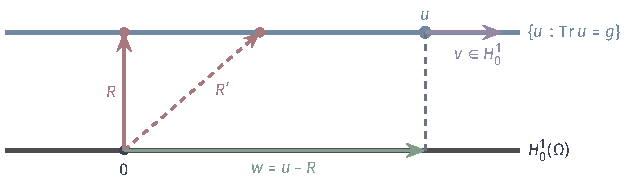
\includegraphics[width=110mm]{figures/06-differential-equations/02-partial-differential-equations/tikz/ellip-affine-trial/figure.pdf}
  \caption{试探集合与测试空间。深灰线是线性空间$H^1_0(\Omega)$，蓝线是平行的试探集合$\{u:\operatorname{Tr}u=g\}$，红色箭头是两个不同的提升$R$与$R'$。解$u$落在蓝线上，$w=u-R$（绿）在$H^1_0(\Omega)$中；试探集合内的移动方向（紫）都属于$H^1_0(\Omega)$，这就是测试函数取自$H^1_0(\Omega)$的原因。}
  \label{fig:ellip-affine-trial}
\end{BookInlineFigure}

提升不唯一，但$u$与提升的选择无关。回到例子$-u''=1$，$u(0)=1$，$u(1)=3$，解是$1+2x+x(1-x)/2$。取$R=1+2x$，得$w=x(1-x)/2$；取$R'=1+2x^2$，得$w'=5x(1-x)/2$。两个$w$不同，$R+w$与$R'+w'$却是同一个函数。

\paragraph{经典解与弱解}
新定义是否与原问题一致？经典解一定是弱解，反过来，足够光滑的弱解也是经典解，下面的定理说明了这一点。

\begin{theorem}[经典解与弱解]
\label{thm:ellip-classical-weak}
设$\Omega$是有界Lipschitz区域，$\bm{A}\in C^1(\overline\Omega)$一致椭圆，$f\in C(\overline\Omega)$，$u\in C^2(\overline\Omega)$，且在$\partial\Omega$上$u=g$。则$u$是弱解当且仅当
\begin{equation}
 -\nabla\cdot(\bm{A}\nabla u)=f\qquad\text{在}\ \Omega\ \text{内逐点成立}.
 \label{eq:ellip-classical}
\end{equation}
\end{theorem}

\begin{proof}
设$u$逐点满足方程。两边乘以$v\in C_c^\infty(\Omega)$，用式~\eqref{eq:ellip-green-first}，边界项为零，得到$a(u,v)=\int fv$。两边对$v$在$H^1$范数下都连续，$C_c^\infty(\Omega)$在$H^1_0(\Omega)$中稠密，所以等式对所有$v\in H^1_0(\Omega)$成立。

反过来，设$u$是弱解。对$v\in C_c^\infty(\Omega)$，式~\eqref{eq:ellip-weak-dirichlet}与式~\eqref{eq:ellip-green-first}合起来给出
\[
 \int_\Omega\bigl(-\nabla\cdot(\bm{A}\nabla u)-f\bigr)v\,\mathrm{d}\bm{x}=0 .
\]
括号内的函数连续。若它在某点不为零，就在该点附近保持同号，取在那里为正的局部凸起$v$，积分不为零，矛盾。所以它处处为零。
\end{proof}

用一个例子看弱形式怎样接纳更粗糙的数据。在$(0,1)$上固定$y$，令$\ell(v)=v(y)$，这是点源。$H^1_0(0,1)$的函数有连续代表，由Cauchy--Schwarz不等式，
\[
 \lvert v(y)\rvert=\Bigl\lvert\int_0^yv'\,\mathrm{d}x\Bigr\rvert\leq\sqrt y\,\lVert v'\rVert_2 ,
\]
所以$\ell$是有界泛函。Green函数$G(\cdot,y)$的斜率在$y$的左右分别是$1-y$和$-y$，代入弱形式，
\[
 \int_0^1G_x\,v'\,\mathrm{d}x=(1-y)\bigl(v(y)-v(0)\bigr)-y\bigl(v(1)-v(y)\bigr)=v(y),
\]
可见帐篷函数就是点源问题的弱解。

一维的这个例子不能推广到高维。$d\geq2$时$H^1$函数不必连续，点值不是有界泛函，点源的解$\Phi$的梯度也不平方可积，这一点在第~\ref{sec:ellip-lax-milgram}小节还会用到。

\subsection{Neumann与Robin条件}
\label{sec:ellip-weak-neumann}

若边界上规定的是通量，式~\eqref{eq:ellip-green-first}的边界项恰好是已知的量，这时不必再让它消失。

\paragraph{Neumann问题}
设$\bm{n}\cdot\bm{A}\nabla u=g$于$\partial\Omega$，$g\in L^2(\partial\Omega)$。两边乘以$v\in H^1(\Omega)$，用式~\eqref{eq:ellip-green-first}，把边界通量换成$g$，移到右端：
\begin{equation}
 a(u,v)=\int_\Omega fv\,\mathrm{d}\bm{x}+\int_{\partial\Omega}gv\,\mathrm{d}S\qquad\text{对所有}\ v\in H^1(\Omega),
 \label{eq:ellip-weak-neumann}
\end{equation}
其中边界积分里的$v$是迹。这里的试探函数和测试函数都在整个$H^1(\Omega)$中，空间没有施加任何边界约束。

\paragraph{Robin问题}
设$\bm{n}\cdot\bm{A}\nabla u+\beta u=g$，$\beta\geq0$。边界通量写成$g-\beta u$，代入后含未知函数$u$的边界项移到左端，得到
\begin{equation}
 a_\beta(u,v)=\int_\Omega fv\,\mathrm{d}\bm{x}+\int_{\partial\Omega}gv\,\mathrm{d}S\qquad\text{对所有}\ v\in H^1(\Omega),
 \label{eq:ellip-weak-robin}
\end{equation}
其中双线性型多了一个边界项：
\begin{equation}
 a_\beta(u,v)=a(u,v)+\int_{\partial\Omega}\beta uv\,\mathrm{d}S.
 \label{eq:ellip-robin-bilinear}
\end{equation}

\paragraph{边界条件怎样从积分中回来}
式~\eqref{eq:ellip-weak-neumann}没有明写边界条件，它是怎样被满足的？设弱解足够光滑。先取$v\in C_c^\infty(\Omega)$，边界项都消失，由定理~\ref{thm:ellip-classical-weak}的论证得到内部方程。

把内部方程代回，对一般的$v\in H^1(\Omega)$，式~\eqref{eq:ellip-green-first}给出
\[
 \int_{\partial\Omega}(\bm{n}\cdot\bm{A}\nabla u-g)\,v\,\mathrm{d}S=0 .
\]
$v$的边界值可以任意变动，所以$\bm{n}\cdot\bm{A}\nabla u=g$成立。这样由弱形式自动产生的条件称为\term{自然边界条件}（natural boundary condition）。对比之下，Dirichlet条件要事先放进试探集合，称为\term{本质边界条件}（essential boundary condition）。

用混合问题看这个机制的效果。方程$-u''=1$，$u(0)=0$，$u'(1)=0$，真解是$u_*=x-x^2/2$。弱形式是：$u$满足$u(0)=0$，且对所有$v(0)=0$的$v\in H^1(0,1)$有$\int_0^1u'v'\,\mathrm{d}x=\int_0^1v\,\mathrm{d}x$。

假如取一个满足内部方程但边界条件错误的候选$\tilde u=x(1-x)/2$，定义残量
\[
 R(v)=\int_0^1\tilde u'v'\,\mathrm{d}x-\int_0^1v\,\mathrm{d}x .
\]
分部积分，因$-\tilde u''=1$，积分项消去，只剩边界项：
\[
 R(v)=\bigl[\tilde u'v\bigr]_0^1=\tilde u'(1)\,v(1)=-\frac{v(1)}2 .
\]

图~\ref{fig:ellip-natural-residual}(b)画出这个关系。只要测试函数在$x=1$处不为零，$\tilde u$就通不过检验，而$u_*$对所有测试函数残量为零。例如$v=x$时，$\tilde u'v'=\tfrac12-x$的积分为$0$，$\int_0^1v=\tfrac12$，所以$R(v)=-\tfrac12$，与公式相符。

\begin{BookInlineFigure}
  \centering
  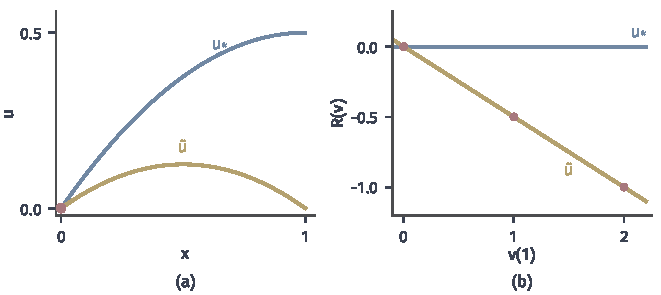
\includegraphics[width=112mm]{figures/06-differential-equations/02-partial-differential-equations/matplotlib/ellip-natural-residual/figure.pdf}
  \caption{自然边界条件由测试函数在边界上的自由度强制。(a)真解$u_*$（蓝）与错误候选$\tilde u$（黄），后者满足$u(1)=0$而不满足$u'(1)=0$。(b)残量$R(v)$随$v(1)$的变化，红点依次是$v=x(1-x)$、$v=x$或$x^2$、$v=2x$；$u_*$的残量恒为零。}
  \label{fig:ellip-natural-residual}
\end{BookInlineFigure}

把两类条件的对比列成表~\ref{tab:ellip-boundary-weak}。三种条件的差异只在于：边界的值由谁来负责。

\begin{BookInlineTable}
  \centering
  \caption{三类边界条件的弱形式。}
  \label{tab:ellip-boundary-weak}
  \begin{tabular}{llll}
    \toprule
    条件 & 试探函数 & 测试函数 & 边界数据的去向\\
    \midrule
    Dirichlet & $\operatorname{Tr}u=g$ & $H^1_0(\Omega)$ & 写进空间（本质）\\
    Neumann & $H^1(\Omega)$ & $H^1(\Omega)$ & 右端边界积分（自然）\\
    Robin & $H^1(\Omega)$ & $H^1(\Omega)$ & 左端$\beta$项与右端积分（自然）\\
    \bottomrule
  \end{tabular}
\end{BookInlineTable}


\section{存在、唯一与稳定性}
\label{sec:ellip-wellposed}

弱形式只是把问题重新写了一遍，解是否存在、是否唯一、是否连续依赖于数据，都还不知道。上一节的三种弱形式有共同的结构：在Hilbert空间$H$中求$u$，使得对所有$v\in H$有$a(u,v)=\ell(v)$。把这个抽象问题解决一次，再逐个边界条件检验假设。

\subsection{Lax--Milgram方法}
\label{sec:ellip-lax-milgram}

先看有限维。考虑方程组$\bm{A}\bm{x}=\bm{b}$，设存在$\alpha>0$，对所有$\bm{x}$有
\[
 \bm{x}^\top\bm{A}\bm{x}\geq\alpha\lVert\bm{x}\rVert_2^2 .
\]
这时矩阵一定可逆，因为$\bm{A}\bm{x}=\bm{0}$推出$\alpha\lVert\bm{x}\rVert_2^2\leq0$。这里不要求$\bm{A}$对称。

下面用一个非对称的矩阵核对：
\[
 \bm{A}=\begin{pmatrix}2&1\\-1&2\end{pmatrix},\qquad\bm{b}=\begin{pmatrix}3\\1\end{pmatrix}.
\]
二次型里的反对称部分互相抵消，$\bm{x}^\top\bm{A}\bm{x}=2\lVert\bm{x}\rVert_2^2$，所以$\alpha=2$。方程的解是$\bm{x}=(1,1)^\top$，并且
\[
 \lVert\bm{x}\rVert_2=\sqrt2\approx1.41\leq\frac{\lVert\bm{b}\rVert_2}{\alpha}=\frac{\sqrt{10}}2\approx1.58 .
\]

这个下界同时给出了可逆性和解的大小，无限维只需把三件事分别补上：把$a$变成算子，由下界得到单射与闭值域，再说明值域没有缺失的方向。第一件事要用Riesz表示定理：Hilbert空间上的每个有界线性泛函都能写成与唯一向量的内积，可参考\BookChapterRef{chap:linear-functionals}{卷四第16章“线性泛函”}。需要的条件如下。

\begin{definition}[有界与强制]
\label{def:ellip-bounded-coercive}
设$H$是实Hilbert空间，$a:H\times H\to\mathbb{R}$是双线性型。若存在$M>0$使
\begin{equation}
 \lvert a(u,v)\rvert\leq M\lVert u\rVert_H\lVert v\rVert_H\qquad\text{对所有}\ u,v\in H,
 \label{eq:ellip-bounded}
\end{equation}
就称$a$有界。若存在$\alpha>0$使
\begin{equation}
 a(v,v)\geq\alpha\lVert v\rVert_H^2\qquad\text{对所有}\ v\in H,
 \label{eq:ellip-coercive}
\end{equation}
就称$a$具有\term{强制性}（coercivity）。
\end{definition}

\begin{theorem}[Lax--Milgram定理]
\label{thm:ellip-lax-milgram}
设$H$是实Hilbert空间，$a$是$H$上有界且强制的双线性型，$\ell\in H^*$。则存在唯一的$u\in H$，使
\begin{equation}
 a(u,v)=\ell(v)\qquad\text{对所有}\ v\in H,
 \label{eq:ellip-abstract}
\end{equation}
并且
\begin{equation}
 \lVert u\rVert_H\leq\frac{\lVert\ell\rVert_{H^*}}{\alpha}.
 \label{eq:ellip-lm-estimate}
\end{equation}
\end{theorem}

\begin{proof}
\emph{第一步，化为算子方程。}由Riesz表示定理，对固定的$u$，$v\mapsto a(u,v)$是有界线性泛函，所以存在唯一的$Tu\in H$，使
\[
 a(u,v)=\langle Tu,v\rangle\qquad\text{对所有}\ v\in H .
\]
同样存在$h\in H$，使$\ell(v)=\langle h,v\rangle$，且$\lVert h\rVert_H=\lVert\ell\rVert_{H^*}$。由$a$的双线性，$T$线性。取$v=Tu$，式~\eqref{eq:ellip-bounded}给出$\lVert Tu\rVert_H\leq M\lVert u\rVert_H$，所以$T$有界。式~\eqref{eq:ellip-abstract}等价于$Tu=h$。

\emph{第二步，下界。}由强制性和Cauchy--Schwarz不等式，
\[
 \alpha\lVert v\rVert_H^2\leq a(v,v)=\langle Tv,v\rangle\leq\lVert Tv\rVert_H\lVert v\rVert_H .
\]
于是
\[
 \lVert Tv\rVert_H\geq\alpha\lVert v\rVert_H\qquad\text{对所有}\ v\in H .
\]
这说明$T$是单射。

\emph{第三步，值域闭。}设$Tv_n\to y$。对差$v_n-v_m$用下界，得到
\[
 \lVert v_n-v_m\rVert_H\leq\frac1\alpha\lVert Tv_n-Tv_m\rVert_H ,
\]
所以$(v_n)$是Cauchy列，收敛到某个$v$。$T$连续，得到$Tv=y$，所以$y$在值域中。

\emph{第四步，值域是全空间。}闭子空间的正交补为零时，子空间就是全空间。设$z$与值域正交。特别地，$z\perp Tz$，于是
\[
 \alpha\lVert z\rVert_H^2\leq a(z,z)=\langle Tz,z\rangle=0 ,
\]
所以$z=0$。因此$T$是双射，$u=T^{-1}h$是唯一的解。

\emph{第五步，估计。}在下界中取$v=u$，得到
\[
 \alpha\lVert u\rVert_H\leq\lVert Tu\rVert_H=\lVert h\rVert_H=\lVert\ell\rVert_{H^*} .
\]
\end{proof}

图~\ref{fig:ellip-lax-milgram}把第三、四步画了出来。下界保证蓝色的值域是闭的，不会缺少极限点；强制性保证与值域垂直的方向$z$不存在，因为若有这样的$z$，$Tz$也在值域中，与$z$垂直，就意味着$a(z,z)=0$。

\begin{BookInlineFigure}
  \centering
  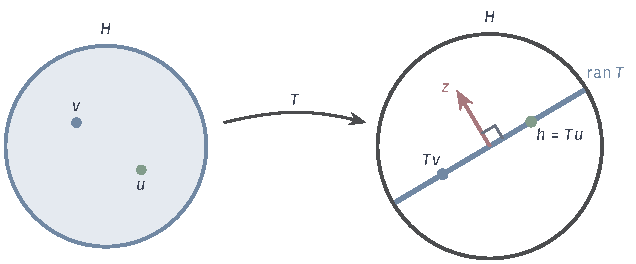
\includegraphics[width=108mm]{figures/06-differential-equations/02-partial-differential-equations/tikz/ellip-lax-milgram/figure.pdf}
  \caption{Lax--Milgram定理证明的几何图景。Riesz表示把$a$变成算子$T$，把$\ell$变成向量$h$，弱问题化为$Tu=h$。下界$\lVert Tv\rVert_H\geq\alpha\lVert v\rVert_H$使值域$\operatorname{ran}T$（蓝线）是闭子空间；红色的$z$若垂直于值域，强制性推出$z=0$，所以值域就是全空间。}
  \label{fig:ellip-lax-milgram}
\end{BookInlineFigure}

\paragraph{各条件的作用}
由式~\eqref{eq:ellip-lm-estimate}，数据之差$\ell_1-\ell_2$导致的解之差满足
\begin{equation}
 \lVert u_1-u_2\rVert_H\leq\frac{\lVert\ell_1-\ell_2\rVert_{H^*}}{\alpha}.
 \label{eq:ellip-lm-stability}
\end{equation}
所以弱问题适定：解存在、唯一，且连续依赖于右端。强制常数$\alpha$越小，同样的数据扰动带来的解的变化可能越大。

三个条件的分工很清楚。有界性让$T$有定义，而且是连续的。强制性同时负责单射、闭值域和满射。$\ell\in H^*$让右端能被表示成向量。

强制性是充分条件，不是必要条件。旋转矩阵$\begin{pmatrix}0&1\\-1&0\end{pmatrix}$可逆，却有$\bm{x}^\top\bm{A}\bm{x}=0$，定理不能用，但这只说明这条路走不通。而在具体方程中，强制性失败时往往确实出了问题：下面的Neumann问题就是这样。

$\ell$有界也不能省略。在$d=2$的单位圆盘上取点源，$\Phi$的梯度大小是$1/(2\pi r)$，能量积分
\[
 \int_{\lVert\bm{x}\rVert_2<1}\lVert\nabla\Phi\rVert_2^2\,\mathrm{d}\bm{x}=\int_0^1\frac{2\pi r}{4\pi^2r^2}\,\mathrm{d}r
\]
对数发散，所以点源问题的解不在$H^1$中。这与“点值不是$H^1_0$上的有界泛函”是同一件事的两面。

\subsection{Dirichlet问题}
\label{sec:ellip-dirichlet}

取$H=H^1_0(\Omega)$。式~\eqref{eq:ellip-uniform}的第二个条件和Cauchy--Schwarz不等式给出有界性：
\[
 \lvert a(u,v)\rvert\leq\kappa_{\max}\lVert\nabla u\rVert_2\lVert\nabla v\rVert_2 .
\]
强制性则要比较$\lVert\nabla v\rVert_2$与$\lVert v\rVert_{H^1}$。式~\eqref{eq:ellip-gradient-control}只控制了梯度，还需要用梯度控制函数本身。

这里需要的工具是Poincaré不等式，由卷四的结论，若$\Omega$有界，存在常数$C_P$，使
\begin{equation}
 \lVert v\rVert_2\leq C_P\lVert\nabla v\rVert_2\qquad\text{对所有}\ v\in H^1_0(\Omega).
 \label{eq:ellip-poincare}
\end{equation}
在$(0,1)$上最优常数是$1/\pi$，它在最低特征函数$\sin(\pi x)$上取到。这个不等式的含义是：函数在边界上被钉在零，要长高就必须爬坡，高度被坡度限制。

由式~\eqref{eq:ellip-poincare}，$\lVert\nabla v\rVert_2$在$H^1_0(\Omega)$上是与$H^1$范数等价的范数，因为
\[
 \lVert\nabla v\rVert_2^2\leq\lVert v\rVert_{H^1}^2\leq(1+C_P^2)\lVert\nabla v\rVert_2^2 .
\]
下面在$H^1_0(\Omega)$上取$\lVert v\rVert_{H^1_0}=\lVert\nabla v\rVert_2$，这时$\alpha=\kappa_{\min}$，$M=\kappa_{\max}$。

\begin{theorem}[Dirichlet问题的适定性]
\label{thm:ellip-dirichlet}
设$\Omega$是有界开集，$\bm{A}$一致椭圆，$f\in L^2(\Omega)$。则$-\nabla\cdot(\bm{A}\nabla u)=f$、零Dirichlet边界的弱解$u\in H^1_0(\Omega)$存在唯一，且
\begin{equation}
 \lVert\nabla u\rVert_2\leq\frac{C_P}{\kappa_{\min}}\lVert f\rVert_2 .
 \label{eq:ellip-dirichlet-estimate}
\end{equation}
若$\Omega$是有界Lipschitz区域，边界值$g=\operatorname{Tr}R$，$R\in H^1(\Omega)$，弱解同样存在唯一，且
\begin{equation}
 \lVert\nabla u\rVert_2\leq\frac{C_P}{\kappa_{\min}}\lVert f\rVert_2+\Bigl(1+\frac{\kappa_{\max}}{\kappa_{\min}}\Bigr)\lVert\nabla R\rVert_2 .
 \label{eq:ellip-dirichlet-inhom}
\end{equation}
\end{theorem}

\begin{proof}
先看$g=0$。令$\ell(v)=\int_\Omega fv\,\mathrm{d}\bm{x}$。由Cauchy--Schwarz不等式和式~\eqref{eq:ellip-poincare}，
\[
 \lvert\ell(v)\rvert\leq\lVert f\rVert_2\lVert v\rVert_2\leq C_P\lVert f\rVert_2\lVert\nabla v\rVert_2 ,
\]
所以$\lVert\ell\rVert\leq C_P\lVert f\rVert_2$。定理~\ref{thm:ellip-lax-milgram}给出唯一的解和估计式~\eqref{eq:ellip-dirichlet-estimate}。

再看一般的$g$。令$u=R+w$，$w$满足式~\eqref{eq:ellip-lifted}。其右端泛函满足
\[
 \Bigl\lvert\int_\Omega fv\,\mathrm{d}\bm{x}-a(R,v)\Bigr\rvert\leq\bigl(C_P\lVert f\rVert_2+\kappa_{\max}\lVert\nabla R\rVert_2\bigr)\lVert\nabla v\rVert_2 .
\]

定理~\ref{thm:ellip-lax-milgram}给出唯一的$w\in H^1_0(\Omega)$，且$\lVert\nabla w\rVert_2$不超过上式括号内的量除以$\kappa_{\min}$。对$u=R+w$用三角不等式，就得到式~\eqref{eq:ellip-dirichlet-inhom}。

唯一性：若$u_1,u_2$都是弱解，差$u_1-u_2\in H^1_0(\Omega)$满足齐次问题，由已证部分为零。
\end{proof}

式~\eqref{eq:ellip-dirichlet-inhom}说明解的大小由源项和边界提升共同决定，并且提升可以取$H^1$范数最小的那一个，于是估计实际上是对边界数据本身的。

用贯穿的例子核对。$\Omega=(0,1)$，$\kappa_{\min}=1$，$C_P=1/\pi$，$f=1$，$\lVert f\rVert_2=1$。解$u=x(1-x)/2$的导数是$1/2-x$，
\[
 \lVert u'\rVert_2=\Bigl(\int_0^1\bigl(\tfrac12-x\bigr)^2\,\mathrm{d}x\Bigr)^{1/2}=\frac1{\sqrt{12}}\approx0.289,
\]
而估计的上界是$1/\pi\approx0.318$，上界成立且相当紧。若取$f=\sin(\pi x)$，解是$\sin(\pi x)/\pi^2$，此时$\lVert u'\rVert_2=\lVert f\rVert_2/\pi$，估计取到等号，这说明常数$C_P/\kappa_{\min}$不能改进。

\paragraph{解算子与特征基}
第~\ref{sec:ellip-spectral}小节留下了一个问题：一般有界区域上，特征函数组成的基存在吗？弱解理论现在可以回答。设$\bm{A}$对称。定义解算子$S:L^2(\Omega)\to L^2(\Omega)$，$Sf$是源项为$f$的弱解。

由式~\eqref{eq:ellip-dirichlet-estimate}，$S$把$L^2$的有界集映为$H^1_0(\Omega)$的有界集。把$H^1_0(\Omega)$的函数零延拓到一个包含$\Omega$的球上，$H^1$有界集到$L^2$的紧嵌入就给出$S$是紧算子。一维时这一紧性更直接：$H^1(a,b)$的有界集由Sobolev不等式一致有界、等度Hölder连续，由Arzelà--Ascoli定理在$C[a,b]$中相对紧，从而在$L^2(a,b)$中相对紧。

$S$还是自伴的。记$u=Sf$，$w=Sh$，把它们互相作为测试函数，由弱形式和$a$的对称性，
\[
 \langle h,Sf\rangle=a(w,u)=a(u,w)=\langle f,Sh\rangle .
\]
$S$也是正的，且是单射，因为$f\neq0$时$u\neq0$，从而$\langle f,Sf\rangle=a(u,u)>0$。

由紧自伴算子的谱定理（可参考\BookChapterRef{chap:operator-spectra}{卷四第18章“算子谱”}），存在$L^2(\Omega)$的标准正交基$(e_k)$，使$Se_k=\mu_ke_k$，$\mu_k>0$，$\mu_k\to0$。令$\lambda_k=1/\mu_k$，则$\lambda_k\to\infty$，$e_k\in H^1_0(\Omega)$，且
\[
 a(e_k,v)=\lambda_k\langle e_k,v\rangle\qquad\text{对所有}\ v\in H^1_0(\Omega) .
\]
这就是特征问题~\eqref{eq:ellip-eigenproblem}的弱形式，而$Sf=\sum_k\mu_kf_ke_k$正是式~\eqref{eq:ellip-spectral-solution}。

\subsection{Neumann问题}
\label{sec:ellip-neumann}

在式~\eqref{eq:ellip-weak-neumann}中取$v=1$，$\nabla v=0$，左端为零，得到
\begin{equation}
 \int_\Omega f\,\mathrm{d}\bm{x}+\int_{\partial\Omega}g\,\mathrm{d}S=0.
 \label{eq:ellip-neumann-compat}
\end{equation}
这是相容条件~\eqref{eq:ellip-interval-compat}的多维形式，意义仍是总量收支为零。不满足这个条件，弱解就不存在。

反过来，$a$在$H^1(\Omega)$上不强制：常数函数$v=1$满足$a(v,v)=0$。若$\Omega$连通，$a(v,v)=0$蕴含$\nabla v=0$，$v$是常数，所以核空间恰好是常数。若$\Omega$不连通，每个连通分支上都可以独立取常数，核空间更大，相容条件也要逐分支成立。

这与奇异矩阵的情形完全相同。图~\ref{fig:ellip-energy-valley}用两个未知量的二次函数$\frac12\bm{c}^\top\bm{K}\bm{c}-\bm{b}^\top\bm{c}$比较三种情形，其极小点满足$\bm{K}\bm{c}=\bm{b}$。(a)是正定的$\bm{K}$，等高线是椭圆，有唯一的极小点。(b)的$\bm{K}=\begin{pmatrix}1&-1\\-1&1\end{pmatrix}$有核方向$(1,1)^\top$，$\bm{b}$与核方向正交时，极小点组成一条线。(c)的$\bm{b}$不与核方向正交，函数沿核方向一直下降，没有极小点。

\begin{BookInlineFigure}
  \centering
  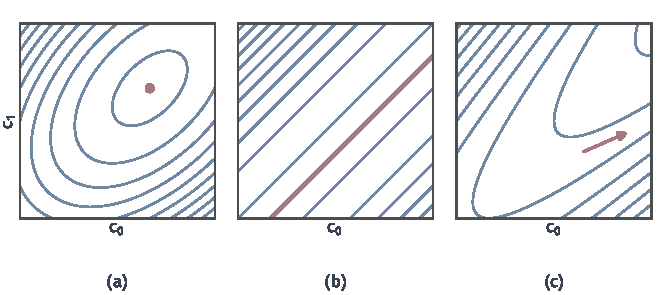
\includegraphics[width=112mm]{figures/06-differential-equations/02-partial-differential-equations/matplotlib/ellip-energy-valley/figure.pdf}
  \caption{核空间的有限维图景，蓝线是$\frac12\bm{c}^\top\bm{K}\bm{c}-\bm{b}^\top\bm{c}$的等高线。(a)$\bm{K}$的对角元为$2$、非对角元为$-1$，$\bm{b}=(1,1)^\top$，唯一极小点$(1,1)$（红）。(b)$\bm{K}$奇异，$\bm{b}=(1,-1)^\top$与核方向$(1,1)^\top$正交，极小点是红线$c_0-c_1=1$。(c)同样的$\bm{K}$，$\bm{b}=(1,0)^\top$，沿红色箭头方向函数无下界。}
  \label{fig:ellip-energy-valley}
\end{BookInlineFigure}

处理办法是先去掉核方向。取零均值子空间
\begin{equation}
 V=\Bigl\{v\in H^1(\Omega):\int_\Omega v\,\mathrm{d}\bm{x}=0\Bigr\}.
 \label{eq:ellip-zero-mean}
\end{equation}
由卷四的零均值Poincaré不等式，在有界连通Lipschitz区域上存在$C_W$，使$\lVert v\rVert_2\leq C_W\lVert\nabla v\rVert_2$对$v\in V$成立。于是$\lVert\nabla\cdot\rVert_2$是$V$上的等价范数，$a$在$V$上强制，$\alpha=\kappa_{\min}$。

迹算子有界，再用上面的等价范数，就存在常数$C_\partial$，使
\begin{equation}
 \lVert\operatorname{Tr}v\rVert_{L^2(\partial\Omega)}\leq C_\partial\lVert\nabla v\rVert_2\qquad\text{对所有}\ v\in V.
 \label{eq:ellip-trace-zero-mean}
\end{equation}

\begin{theorem}[Neumann问题的适定性]
\label{thm:ellip-neumann}
设$\Omega$是有界连通Lipschitz区域，$\bm{A}$一致椭圆，$f\in L^2(\Omega)$，$g\in L^2(\partial\Omega)$。式~\eqref{eq:ellip-weak-neumann}有解当且仅当式~\eqref{eq:ellip-neumann-compat}成立。此时解在相差一个常数的意义下唯一，零均值的解$u\in V$满足
\begin{equation}
 \lVert\nabla u\rVert_2\leq\frac1{\kappa_{\min}}\bigl(C_W\lVert f\rVert_2+C_\partial\lVert g\rVert_{L^2(\partial\Omega)}\bigr).
 \label{eq:ellip-neumann-estimate}
\end{equation}
\end{theorem}

\begin{proof}
必要性已经证明。设相容条件成立，令$\ell(v)=\int_\Omega fv+\int_{\partial\Omega}gv$。在$V$上，由Cauchy--Schwarz不等式和式~\eqref{eq:ellip-trace-zero-mean}，
\[
 \lvert\ell(v)\rvert\leq\bigl(C_W\lVert f\rVert_2+C_\partial\lVert g\rVert_{L^2(\partial\Omega)}\bigr)\lVert\nabla v\rVert_2 .
\]
定理~\ref{thm:ellip-lax-milgram}给出唯一的$u\in V$和估计式~\eqref{eq:ellip-neumann-estimate}，它对所有$v\in V$满足$a(u,v)=\ell(v)$。

还要把测试函数从$V$扩大到$H^1(\Omega)$。任取$v\in H^1(\Omega)$，令$\bar v=\lvert\Omega\rvert^{-1}\int_\Omega v$，则$v-\bar v\in V$。$a(u,\bar v)=0$，因为常数的梯度为零；$\ell(\bar v)=0$，因为相容条件成立。于是
\[
 a(u,v)=a(u,v-\bar v)=\ell(v-\bar v)=\ell(v) .
\]

若$u_1,u_2$都是解，差$z=u_1-u_2$满足$a(z,z)=0$，由式~\eqref{eq:ellip-gradient-control}，$\nabla z=0$，$\Omega$连通，故$z$是常数。
\end{proof}

用前面的例子核对。$\Omega=(0,1)$，$f=1-2x$，$C_W=1/\pi$，$\lVert f\rVert_2=1/\sqrt3$。解的导数$u'=x^2-x$，
\[
 \lVert u'\rVert_2=\Bigl(\int_0^1(x^2-x)^2\,\mathrm{d}x\Bigr)^{1/2}=\frac1{\sqrt{30}}\approx0.183,
\]
上界$C_W\lVert f\rVert_2=1/(\pi\sqrt3)\approx0.184$，几乎取到等号，因为$f$很接近第一个非常数的特征函数。

这里的估计式~\eqref{eq:ellip-neumann-estimate}只对零均值的代表成立，也只能如此：加上常数后，解可以任意大，却仍是解。

\subsection{Robin问题}
\label{sec:ellip-robin}

Robin问题的$a_\beta$比$a$多了边界项$\int_{\partial\Omega}\beta v^2$。常数函数在$a$中的能量为零，在这里要付出边界代价。边界项能否像Poincaré不等式那样补足对函数本身的控制？

先看一个可以直接解的例子。在$(0,1)$上取$-u''=1$，两端都是$\bm{n}\cdot\nabla u+\beta u=0$，$\beta>0$。由对称性，解形如$x(1-x)/2+c$，代入左端条件：
\[
 -u'(0)+\beta u(0)=-\frac12+\beta c=0 ,
\]
所以
\begin{equation}
 u(x)=\frac{x(1-x)}2+\frac1{2\beta}.
 \label{eq:ellip-robin-example}
\end{equation}

图~\ref{fig:ellip-robin-beta}显示$\beta$的作用。$\beta\to\infty$时，边界换热无限快，解收敛到Dirichlet问题的解。$\beta\to0$时，$u$的常数部分$1/(2\beta)$趋于无穷，解的范数爆炸；极限的Neumann问题$f=1$本来就不相容。收支也是平衡的：总产热$1$经两端散出，$\beta(u(0)+u(1))=1$。

\begin{BookInlineFigure}
  \centering
  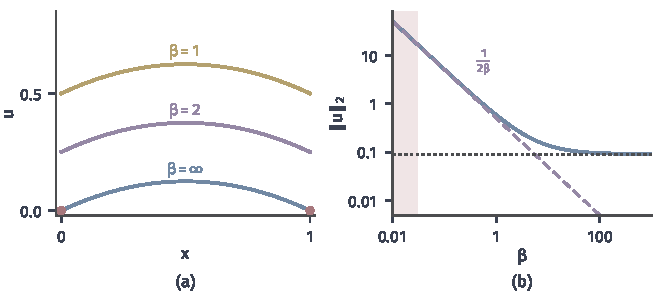
\includegraphics[width=112mm]{figures/06-differential-equations/02-partial-differential-equations/matplotlib/ellip-robin-beta/figure.pdf}
  \caption{$-u''=1$、两端Robin条件的解。(a)$\beta=1,2$时（黄、紫）解被整体抬高$1/(2\beta)$，$\beta\to\infty$时趋于蓝线的Dirichlet解。(b)$\lVert u\rVert_2$随$\beta$的变化：$\beta\to0$时沿紫色虚线$1/(2\beta)$爆炸（红底区域接近不相容的Neumann极限），$\beta\to\infty$时趋于点线$1/\sqrt{120}$。}
  \label{fig:ellip-robin-beta}
\end{BookInlineFigure}

这个例子说明，强制常数必然随$\beta$退化，所以需要一条统一的不等式，把$\beta$的作用写进去。

\begin{lemma}[边界项给出的Poincaré不等式]
\label{lem:ellip-robin-poincare}
设$\Omega$是有界连通Lipschitz区域，$\beta\in L^\infty(\partial\Omega)$，$\beta\geq0$，$\int_{\partial\Omega}\beta\,\mathrm{d}S>0$。则存在常数$C_R$，使
\begin{equation}
 \lVert v\rVert_2^2\leq C_R\Bigl(\lVert\nabla v\rVert_2^2+\int_{\partial\Omega}\beta v^2\,\mathrm{d}S\Bigr)\qquad\text{对所有}\ v\in H^1(\Omega).
 \label{eq:ellip-robin-poincare}
\end{equation}
\end{lemma}

\begin{proof}
用反证法。若不等式不成立，存在序列$(v_n)\subset H^1(\Omega)$，$\lVert v_n\rVert_2=1$，并且
\[
 \lVert\nabla v_n\rVert_2^2+\int_{\partial\Omega}\beta v_n^2\,\mathrm{d}S\to0 .
\]
序列在$H^1$中有界，由$H^1(\Omega)$到$L^2(\Omega)$的紧嵌入，有子列在$L^2(\Omega)$中收敛到某个$v$，$\lVert v\rVert_2=1$。子列的梯度趋于零，所以子列在$H^1$中也是Cauchy列，收敛到$v$，且$\nabla v=0$。

$\Omega$连通，所以$v$等于常数$c$，由$\lVert v\rVert_2=1$知$c\neq0$。迹算子连续，$\operatorname{Tr}v_n\to c$于$L^2(\partial\Omega)$，$\beta$有界，于是
\[
 \int_{\partial\Omega}\beta v_n^2\,\mathrm{d}S\to c^2\int_{\partial\Omega}\beta\,\mathrm{d}S>0 ,
\]
这与假设矛盾。
\end{proof}

这个证明用了紧嵌入，所以常数$C_R$是非构造性的。证明的核心很直白：能让所有控制量都趋于零的只有常数，而边界上正的$\beta$排除了常数。

\begin{theorem}[Robin问题的适定性]
\label{thm:ellip-robin}
设$\Omega$是有界连通Lipschitz区域，$\bm{A}$一致椭圆，$\beta$满足引理~\ref{lem:ellip-robin-poincare}的条件，$f\in L^2(\Omega)$，$g\in L^2(\partial\Omega)$。则式~\eqref{eq:ellip-weak-robin}存在唯一的解$u\in H^1(\Omega)$，且存在只依赖于$\Omega,\bm{A},\beta$的常数$C$，使
\begin{equation}
 \lVert u\rVert_{H^1}\leq C\bigl(\lVert f\rVert_2+\lVert g\rVert_{L^2(\partial\Omega)}\bigr).
 \label{eq:ellip-robin-estimate}
\end{equation}
\end{theorem}

\begin{proof}
由迹定理，存在$C_{\mathrm{Tr}}$，使
\[
 \lVert\operatorname{Tr}v\rVert_{L^2(\partial\Omega)}\leq C_{\mathrm{Tr}}\lVert v\rVert_{H^1} .
\]
于是$a_\beta$有界：
\[
 \lvert a_\beta(u,v)\rvert\leq\bigl(\kappa_{\max}+\lVert\beta\rVert_\infty C_{\mathrm{Tr}}^2\bigr)\lVert u\rVert_{H^1}\lVert v\rVert_{H^1} .
\]
右端泛函也有界，其范数不超过$\lVert f\rVert_2+C_{\mathrm{Tr}}\lVert g\rVert_{L^2(\partial\Omega)}$。

由式~\eqref{eq:ellip-gradient-control}，令$\kappa_0=\min(\kappa_{\min},1)$，
\[
 a_\beta(v,v)\geq\kappa_0\Bigl(\lVert\nabla v\rVert_2^2+\int_{\partial\Omega}\beta v^2\,\mathrm{d}S\Bigr) .
\]
由式~\eqref{eq:ellip-robin-poincare}，
\[
 \lVert v\rVert_{H^1}^2\leq(1+C_R)\Bigl(\lVert\nabla v\rVert_2^2+\int_{\partial\Omega}\beta v^2\,\mathrm{d}S\Bigr) .
\]
所以$a_\beta$强制，$\alpha=\kappa_0/(1+C_R)$。定理~\ref{thm:ellip-lax-milgram}给出结论。
\end{proof}

条件$\int_{\partial\Omega}\beta>0$不能去掉。$\beta\equiv0$时问题退回Neumann问题，核空间是常数，唯一性丢失。条件$\beta\geq0$也不能随意放宽。在$(0,1)$上取两端$\beta=-2$，考察$-u''=0$，函数$u=1-2x$满足
\[
 -u'(0)+\beta u(0)=2-2=0,\qquad u'(1)+\beta u(1)=-2+2=0 ,
\]
这是一个非零的解，所以齐次问题不唯一。负的$\beta$相当于边界不断向棒内放热，且放热量随温度增长，边界项不再贡献能量，而是削弱能量。

三类边界条件的结论可以这样总结：Dirichlet问题靠零迹排除常数，Robin问题靠边界代价排除常数，Neumann问题排除不了常数，只能把常数方向分离出去，并要求数据与之相容。


\section{能量极小}
\label{sec:ellip-energy}

一根绷紧的弦受到载荷后停在某个形状，这个形状是所有可能形状中总势能最小的。Poisson方程的弱解是否也是某种能量的极小点？第~\ref{sec:ellip-wellposed}节的三种弱形式都能这样解释吗？

\paragraph{能量泛函}
对$H$上的双线性型$a$和右端泛函$\ell$，定义二次泛函
\begin{equation}
 J(v)=\frac12a(v,v)-\ell(v).
 \label{eq:ellip-energy}
\end{equation}
对Dirichlet问题，$a$和$\ell$分别是式~\eqref{eq:ellip-bilinear}与$\int_\Omega fv$，所以
\[
 J(v)=\frac12\int_\Omega\bm{A}\nabla v\cdot\nabla v\,\mathrm{d}\bm{x}-\int_\Omega fv\,\mathrm{d}\bm{x} .
\]
第一项是梯度的储能，第二项是载荷做功的相反数，两者折中，形成平衡。

有限维的类比是对称正定的$\bm{K}$和二次函数$\frac12\bm{c}^\top\bm{K}\bm{c}-\bm{b}^\top\bm{c}$，令梯度为零，正是$\bm{K}\bm{c}=\bm{b}$。下面的定理是这件事的无限维版本。泛函的方向导数与极小点的一般理论可参考\BookChapterRef{chap:functional-optimization-variation}{卷五第29章“泛函优化”}，这里的二次泛函可以直接展开，不需要一般理论。

\begin{theorem}[弱解是能量的唯一极小点]
\label{thm:ellip-energy}
设$H$是实Hilbert空间，$a$是$H$上有界、强制且对称的双线性型，$\ell\in H^*$。对$u\in H$，下面两条等价：
\begin{enumerate}
 \item $a(u,v)=\ell(v)$对所有$v\in H$成立；
 \item $u$是$J$在$H$上的极小点。
\end{enumerate}
极小点存在且唯一，并且对所有$w\in H$，
\begin{equation}
 J(u+w)-J(u)=\frac12a(w,w).
 \label{eq:ellip-energy-gap}
\end{equation}
\end{theorem}

\begin{proof}
对任意$u,w\in H$，由双线性与对称性展开，
\[
 J(u+w)=J(u)+\bigl(a(u,w)-\ell(w)\bigr)+\frac12a(w,w).
\]

设第1条成立，括号为零，就得到式~\eqref{eq:ellip-energy-gap}。由强制性，$w\neq0$时$a(w,w)>0$，所以$u$是唯一的极小点。

设第2条成立。任取$v\in H$和实数$t$，取$w=tv$，极小性给出
\[
 0\leq J(u+tv)-J(u)=t\bigl(a(u,v)-\ell(v)\bigr)+\frac{t^2}2a(v,v).
\]
右端是$t$的二次函数，在$t=0$处取最小值$0$，所以一次项系数为零，即第1条成立。

极小点的存在由定理~\ref{thm:ellip-lax-milgram}给出。
\end{proof}

式~\eqref{eq:ellip-energy-gap}比“极小”的说法更强：任何候选的能量超出最优能量的部分，恰好是它到解的距离在能量范数下的平方的一半。

对称情形下，存在性也可以不用Lax--Milgram定理。此时$a(\cdot,\cdot)$本身是$H$上的一个等价内积，Riesz表示定理直接给出解；或者取极小化序列用平行四边形恒等式证明它是Cauchy列。这是对称问题的简化，非对称问题走不通。

\paragraph{手算比较}
继续用$-u''=1$，$u(0)=u(1)=0$，这时$J(v)=\frac12\int_0^1v'^2-\int_0^1v$。把真解$u_*=x(1-x)/2$代入：
\[
 J(u_*)=\frac12\cdot\frac1{12}-\frac1{12}=-\frac1{24}\approx-0.04167 .
\]

取几个其他的候选比较，都先把幅度调到各自的最优值。形如$cx(1-x)$的候选有
\[
 J=\frac{c^2}6-\frac c6,
\]
它在$c=1/2$处最小，正好回到真解。帐篷函数$s\min(x,1-x)$有$J=s^2/2-s/4$，最优幅度$s=1/4$给出$J=-1/32\approx-0.03125$。单个正弦$c\sin(\pi x)$的最优幅度是$c=4/\pi^3$，给出$J=-4/\pi^4\approx-0.04106$。

\begin{BookInlineFigure}
  \centering
  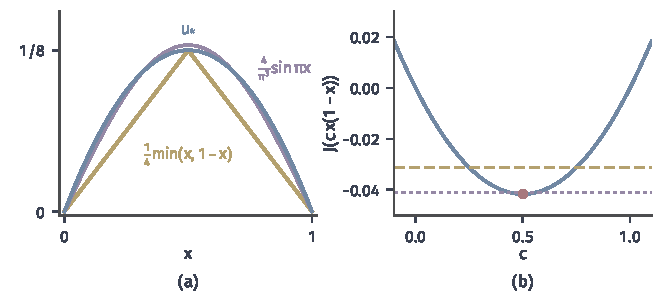
\includegraphics[width=112mm]{figures/06-differential-equations/02-partial-differential-equations/matplotlib/ellip-energy-competition/figure.pdf}
  \caption{能量比较，$f=1$，零边界。(a)真解$u_*$（蓝）与两个候选：帐篷（黄）和单个正弦（紫）。(b)蓝线是$J(cx(1-x))$，红点是$c=1/2$处的最小值$-1/24$；黄色虚线和紫色点线分别是帐篷和正弦的能量，都高于$-1/24$。}
  \label{fig:ellip-energy-competition}
\end{BookInlineFigure}

图~\ref{fig:ellip-energy-competition}表明，正弦候选的形状已经非常接近真解，能量也只比最优高$0.0006$。式~\eqref{eq:ellip-energy-gap}解释了能量如此接近的原因：能量差是误差的平方，误差小时，能量差更小。

\paragraph{边界条件的归宿}
能量泛函还给出了本质边界条件与自然边界条件的另一种解释。Dirichlet问题的约束是对可行集的限制，要在集合$\{v\in H^1(\Omega):\operatorname{Tr}v=g\}$上极小化。Neumann问题没有约束，$J$里多一项$-\int_{\partial\Omega}gv$，边界条件是极小性自己产生的。Robin问题里，$\frac12\int_{\partial\Omega}\beta v^2$是边界代价，$\beta\to\infty$时迫使$v$在边界上趋于零，这正是图~\ref{fig:ellip-robin-beta}看到的极限。

Neumann问题的能量沿常数方向是平的，这就是图~\ref{fig:ellip-energy-valley}的情形：相容条件成立时极小点组成一条直线，不成立时能量沿常数方向无下界，极小点不存在。

\paragraph{非对称问题}
对称性不能省去。考虑带一阶项的方程$-u''+bu'=f$，$u(0)=u(1)=0$，$b$是常数。在$H^1_0(0,1)$上，弱形式的双线性型是
\begin{equation}
 a_b(u,v)=\int_0^1u'v'\,\mathrm{d}x+b\int_0^1u'v\,\mathrm{d}x .
 \label{eq:ellip-convection-form}
\end{equation}

它有界，因为由Poincaré不等式，
\[
 \Bigl\lvert b\int_0^1u'v\,\mathrm{d}x\Bigr\rvert\leq\lvert b\rvert\lVert u'\rVert_2\lVert v\rVert_2\leq\frac{\lvert b\rvert}\pi\lVert u'\rVert_2\lVert v'\rVert_2 .
\]
它也强制，而且强制常数与$b$无关：
\[
 \int_0^1v'v\,\mathrm{d}x=\frac12\bigl[v^2\bigr]_0^1=0,\qquad\text{所以}\quad a_b(v,v)=\lVert v'\rVert_2^2 .
\]
由Lax--Milgram定理，弱解存在唯一。$f=1$时可以解出
\begin{equation}
 u_b(x)=\frac xb-\frac{\mathrm{e}^{bx}-1}{b(\mathrm{e}^b-1)},\qquad b\neq0 .
 \label{eq:ellip-convection-solution}
\end{equation}

这个解不是$J(v)=\frac12a_b(v,v)-\ell(v)$的极小点。由上式，$\frac12a_b(v,v)=\frac12\lVert v'\rVert_2^2$，$b$根本没有出现在$J$中。$J$的极小点对每个$b$都是$b=0$的解$x(1-x)/2$，而图~\ref{fig:ellip-nonsymmetric}中真正的解随$b$的增大明显向右偏移。

一般地，$J$在$u$处沿$w$的变化率是$\frac12(a(u,w)+a(w,u))-\ell(w)$，只看到$a$的对称部分。

\begin{BookInlineFigure}
  \centering
  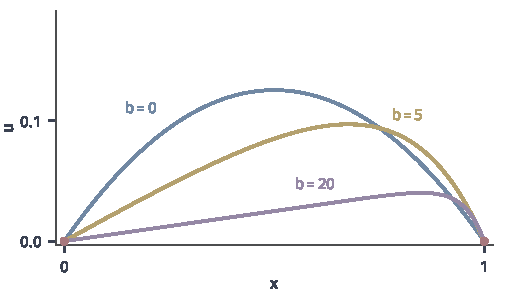
\includegraphics[width=86mm]{figures/06-differential-equations/02-partial-differential-equations/matplotlib/ellip-nonsymmetric/figure.pdf}
  \caption{非对称问题$-u''+bu'=1$的解随$b$的变化。$b=0$（蓝）时对称，$b=5$（黄）与$b=20$（紫）时被对流推向右端，在$x=1$附近形成边界层。双线性型的二次部分与$b$无关，所以这些解不能由式~\eqref{eq:ellip-energy}的极小化得到。}
  \label{fig:ellip-nonsymmetric}
\end{BookInlineFigure}

区间上的这个例子还可以用积分因子补救。在方程两边乘以$\mathrm{e}^{-bx}$，得到$-(\mathrm{e}^{-bx}u')'=\mathrm{e}^{-bx}f$，它在带权的能量下又是对称的。多维情形中，只有当一阶项的系数是某个函数的梯度时，这种办法才能奏效，否则一般不存在把问题化成能量极小的权函数。所以结论是：Lax--Milgram定理适用的范围比能量极小更广，能量极小只是对称情形的额外结构。


\section{最大值原理}
\label{sec:ellip-maximum}

前面的能量估计控制的是平方积分的大小，没有告诉我们解在哪里最大。温度分布有一个直观的事实：没有内部热源时，最高温只能出现在边界上。若内部出现了一个比周围都热的点，热量就会从它流向四周，无法平衡。把这个直觉变成定理，需要用到方程的符号结构。

\paragraph{调和函数是平均值}
上面的直觉有一个精确的版本：调和函数在每一点的值，等于以该点为心的任意球面上的平均值，这称为\term{平均值性质}（mean value property）。

\begin{theorem}[平均值性质]
\label{thm:ellip-mean-value}
设$u\in C^2(\Omega)$在$\Omega$内调和，$\overline{B_r(\bm{x})}\subset\Omega$。则
\begin{equation}
 u(\bm{x})=\frac1{\lvert\partial B_r\rvert}\int_{\partial B_r(\bm{x})}u\,\mathrm{d}S,
 \label{eq:ellip-mean-value}
\end{equation}
并且对球体上的平均，同样的等式成立。
\end{theorem}

\begin{proof}
把球面积分写成单位球面$S$上的平均，令
\[
 m(r)=\frac1{\lvert S\rvert}\int_Su(\bm{x}+r\bm{\omega})\,\mathrm{d}\sigma(\bm{\omega}) .
\]
对$r$求导，换回半径$r$的球面，并用散度定理：
\[
 m'(r)=\frac1{\lvert\partial B_r\rvert}\int_{\partial B_r}\partial_{\bm{n}}u\,\mathrm{d}S=\frac1{\lvert\partial B_r\rvert}\int_{B_r}\Delta u\,\mathrm{d}\bm{y}=0 .
\]
所以$m$是常数，又因$u$连续，$r\to0$时$m(r)\to u(\bm{x})$。这就证明了式~\eqref{eq:ellip-mean-value}。球体上的平均是不同半径的球面平均对$r$的加权积分，也等于$u(\bm{x})$。
\end{proof}

图~\ref{fig:ellip-harmonic-saddle}中，$u=x_1^2-x_2^2$在圆盘上调和。圆周上的值有高有低，平均后恰好是圆心的值。这个函数的最大值出现在边界上的两个红点，最小值在两个紫点，内部的鞍点不是极值。

\begin{BookInlineFigure}
  \centering
  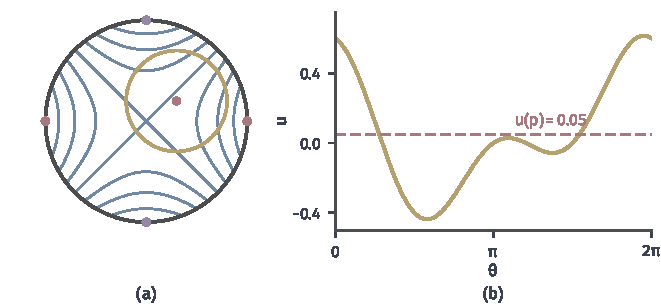
\includegraphics[width=112mm]{figures/06-differential-equations/02-partial-differential-equations/matplotlib/ellip-harmonic-saddle/figure.pdf}
  \caption{调和函数$u=x_1^2-x_2^2$。(a)单位圆盘内的等值线，红点是边界上的最大值点，紫点是最小值点。黄圆心在$\bm{p}=(0.3,0.2)$，半径$0.5$。(b)黄圆上$u$的取值（黄），红色虚线是圆心值$u(\bm{p})=0.05$，也是这些取值的平均值。}
  \label{fig:ellip-harmonic-saddle}
\end{BookInlineFigure}

\paragraph{Laplace算子的最大值原理}
把“内部的值不超过边界上的值”写成定理，就是\term{最大值原理}（maximum principle）。它只要求$-\Delta u\leq0$，即区域内部没有热源，但可以有热汇。

\begin{theorem}[弱最大值原理]
\label{thm:ellip-weak-max}
设$\Omega$是有界开集，$u\in C^2(\Omega)\cap C(\overline\Omega)$，在$\Omega$内$-\Delta u\leq0$。则
\begin{equation}
 \max_{\overline\Omega}u=\max_{\partial\Omega}u.
 \label{eq:ellip-weak-max}
\end{equation}
\end{theorem}

\begin{proof}
先处理严格的情形。若$-\Delta v<0$，$v$不可能在内部取最大值：在内部最大值点，每个方向的二阶导数都不超过零，$\Delta v\leq0$，与$\Delta v>0$矛盾。

对一般的$u$，令$v_\varepsilon=u+\varepsilon\lVert\bm{x}\rVert_2^2$，$\varepsilon>0$。则$\Delta v_\varepsilon=\Delta u+2d\varepsilon>0$，所以$v_\varepsilon$的最大值在边界上取得，于是
\[
 \max_{\overline\Omega}u\leq\max_{\overline\Omega}v_\varepsilon=\max_{\partial\Omega}v_\varepsilon\leq\max_{\partial\Omega}u+\varepsilon\max_{\partial\Omega}\lVert\bm{x}\rVert_2^2 .
\]
令$\varepsilon\to0$，得到$\max_{\overline\Omega}u\leq\max_{\partial\Omega}u$。反向不等式由$\partial\Omega\subset\overline\Omega$得到。
\end{proof}

定理说最大值在边界上取得，但不排除内部也取到。调和函数的情形可以说得更多：若$\Omega$连通，调和函数在内部取到最大值，则必为常数。设最大值$M$在内部某点取到，集合$\{u=M\}$在$\Omega$中闭。由球上的平均值性质，若$u(\bm{x})=M$，球内$u\leq M$而平均等于$M$，只能处处等于$M$，所以这个集合又是开的。连通性使它等于整个$\Omega$。这是强最大值原理在调和情形的证明。

\paragraph{比较与上界}
最大值原理最直接的用途是比较两个解。把定理用于差$u-w$，得到\term{比较原理}（comparison principle），再选择不同的比较函数，就有下面三个结论。

\begin{theorem}[比较原理与上界]
\label{thm:ellip-comparison}
设$\Omega$是有界开集，$u,w\in C^2(\Omega)\cap C(\overline\Omega)$。
\begin{enumerate}
 \item 若在$\Omega$内$-\Delta u\leq-\Delta w$，在$\partial\Omega$上$u\leq w$，则在$\Omega$内$u\leq w$。
 \item Poisson方程的Dirichlet问题最多有一个$C^2(\Omega)\cap C(\overline\Omega)$解。
 \item 设$\Omega\subset B_\rho(\bm{x}_0)$，$-\Delta u=f$，$u=g$于$\partial\Omega$，且$f$有界。则
 \begin{equation}
 \max_{\overline\Omega}\lvert u\rvert\leq\max_{\partial\Omega}\lvert g\rvert+\frac{\rho^2}{2d}\sup_\Omega\lvert f\rvert .
 \label{eq:ellip-max-bound}
 \end{equation}
\end{enumerate}
\end{theorem}

\begin{proof}
第1条，$z=u-w$满足$-\Delta z\leq0$，由定理~\ref{thm:ellip-weak-max}，$\max z=\max_{\partial\Omega}z\leq0$。第2条，两个解的差$z$满足$\Delta z=0$且边界值为零，把定理用于$z$与$-z$，得到$z=0$。

第3条，记$F=\sup\lvert f\rvert$，$G_0=\max_{\partial\Omega}\lvert g\rvert$。取比较函数
\[
 w(\bm{x})=G_0+\frac F{2d}\bigl(\rho^2-\lVert\bm{x}-\bm{x}_0\rVert_2^2\bigr).
\]
由$\Delta\lVert\bm{x}\rVert_2^2=2d$，$-\Delta w=F\geq\pm f$，并且$\overline\Omega$上$w\geq G_0\geq\pm g$。第1条分别用于$u$和$-u$，得到$\lvert u\rvert\leq w\leq G_0+F\rho^2/(2d)$。
\end{proof}

检验一下估计的精度。$\Omega=(0,1)$，$d=1$，$\rho=1/2$，$\bm{x}_0=1/2$，$f=1$，$g=0$，式~\eqref{eq:ellip-max-bound}给出$\lvert u\rvert\leq1/8$，恰好等于真解的最大值。这里比较函数$w=\frac12(\frac14-(x-\frac12)^2)=x(1-x)/2$就是真解本身。

比较原理还告诉我们，$f\geq0$且$g\geq0$时$u\geq0$，即加热不会使温度降低。这对点源同样成立，所以Green函数非负：$G(\bm{x},\bm{y})\geq0$，在式~\eqref{eq:ellip-green-1d}中也能直接看出来。

\paragraph{带低阶项的算子}
考虑更一般的算子，写成非散度形式
\begin{equation}
 Lu=-\operatorname{tr}\bigl(\bm{A}\nabla^2u\bigr)+\bm{b}\cdot\nabla u+cu,
 \label{eq:ellip-general-operator}
\end{equation}
其中$\bm{A}(\bm{x})$对称，满足式~\eqref{eq:ellip-uniform}，$\bm{b}$和$c$在$\Omega$上有界，$\nabla^2u$是Hessian矩阵。式~\eqref{eq:ellip-divergence-form}在$\bm{A}\in C^1$时也能写成这个形式。

最大值原理成立的关键是$c$的符号。在正的最大值点，$\nabla u=0$，$\nabla^2u$半负定，所以$-\operatorname{tr}(\bm{A}\nabla^2u)\geq0$。若$c\geq0$，还有$cu\geq0$，两项都迫使$Lu\geq0$，这与$Lu<0$矛盾。

\begin{theorem}[带零阶项的最大值原理]
\label{thm:ellip-general-max}
设$\Omega$是有界开集，$L$如式~\eqref{eq:ellip-general-operator}，$c\geq0$。若$u\in C^2(\Omega)\cap C(\overline\Omega)$满足$Lu\leq0$，则
\begin{equation}
 \max_{\overline\Omega}u\leq\max_{\partial\Omega}u^+,
 \label{eq:ellip-general-max}
\end{equation}
其中$u^+=\max(u,0)$。若$c\equiv0$，则$\max_{\overline\Omega}u=\max_{\partial\Omega}u$。
\end{theorem}

\begin{proof}
先设$c\equiv0$，记此时的算子为$L_0$。若$L_0v<0$，由上面的论证，$v$在内部没有最大值点。一般情形下取$\gamma$足够大，令$\psi=\mathrm{e}^{\gamma x_1}$，有
\[
 L_0\psi=\bigl(-A_{1,1}\gamma^2+b_1\gamma\bigr)\psi\leq\gamma\bigl(-\kappa_{\min}\gamma+\lVert\bm{b}\rVert_\infty\bigr)\psi<0 .
\]
于是$v_\varepsilon=u+\varepsilon\psi$满足$L_0v_\varepsilon<0$，最大值在边界上取得。令$\varepsilon\to0$，与定理~\ref{thm:ellip-weak-max}的做法相同，得到结论。

再看$c\geq0$。若$u\leq0$，式~\eqref{eq:ellip-general-max}已成立。否则令$\Omega^+=\{\bm{x}\in\Omega:u(\bm{x})>0\}$。在这个开集上$L_0u=Lu-cu\leq0$，把已证结论用于$\Omega^+$。$\Omega^+$的边界点要么在$\partial\Omega$上，要么满足$u=0$，所以$u$的最大值不超过$\max_{\partial\Omega}u^+$。
\end{proof}

图~\ref{fig:ellip-sign-failure}显示$c$的两种符号。(a)中$c\geq0$，$-u''+cu=1$，$u(0)=u(1)=0$。常数函数$w=1/c$满足$Lw=1$，边界上$w>u$，由比较原理（对差$u-w$用定理~\ref{thm:ellip-general-max}）得到$u\leq1/c$，图中的点线就是这个上界。$c$越大，方程越像$cu=1$，解越贴近$1/c$。

(b)中$c=-\pi^2$，方程$-u''-\pi^2u=0$有非零解$A\sin(\pi x)$，它们的边界值都是零，内部却有非零的值，最大值原理和唯一性同时失效。这里$-\pi^2$恰好是$-\lambda_1$，用谱展开的语言说，算子有了零特征值。

\begin{BookInlineFigure}
  \centering
  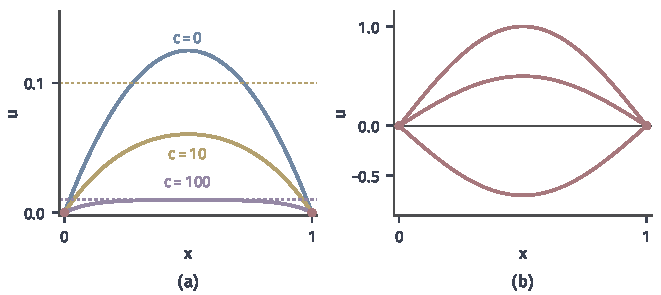
\includegraphics[width=112mm]{figures/06-differential-equations/02-partial-differential-equations/matplotlib/ellip-sign-failure/figure.pdf}
  \caption{零阶项的符号。(a)$-u''+cu=1$，零边界，$c=0,10,100$，点线是上界$u\leq1/c$（$c=0$时无此上界）。(b)$c=-\pi^2$时$u=A\sin(\pi x)$（红线，$A=1,\tfrac12,-\tfrac7{10}$）都满足齐次方程和零边界，最大值原理失效。}
  \label{fig:ellip-sign-failure}
\end{BookInlineFigure}

\paragraph{弱解的最大值原理}
定理~\ref{thm:ellip-general-max}要求$u\in C^2$。散度型方程的弱解有一个不需要二阶导数的版本，它把能量方法和最大值原理连在了一起。

设$u\in H^1(\Omega)$是式~\eqref{eq:ellip-divergence-form}的弱解，$f\leq0$，$\operatorname{Tr}u\leq M$。把$v=(u-M)^+$作为测试函数，这里用到$H^1$函数被截断后仍在$H^1$中，且$\nabla v=\nabla u\,\mathbf{1}_{\{u>M\}}$，$v$的迹为零，所以$v\in H^1_0(\Omega)$。

由弱形式和$f\leq0$，$v\geq0$，
\[
 \kappa_{\min}\lVert\nabla v\rVert_2^2\leq\int_\Omega\bm{A}\nabla v\cdot\nabla v\,\mathrm{d}\bm{x}=a(u,v)=\int_\Omega fv\,\mathrm{d}\bm{x}\leq0 .
\]
所以$\nabla v=0$，由Poincaré不等式$v=0$，即$u\leq M$几乎处处成立。这个证明不要求$\bm{A}$连续，也适用于前面那根两段材料的棒。

\paragraph{两种估计的对比}
能量估计与最大值估计回答不同的问题，见表~\ref{tab:ellip-energy-vs-max}。两者不能互相替代：弱解的能量估计不给出逐点的界，而最大值原理不给出梯度的积分界。

\begin{BookInlineTable}
  \centering
  \caption{能量估计与最大值估计的对比。}
  \label{tab:ellip-energy-vs-max}
  \begin{tabular}{lll}
    \toprule
    & 能量估计 & 最大值估计\\
    \midrule
    控制的量 & $\lVert\nabla u\rVert_2$（平方平均） & $\max\lvert u\rvert$（逐点）\\
    数据的度量 & $\lVert f\rVert_2$ & $\sup\lvert f\rvert$\\
    结构要求 & 强制性 & 符号（$c\geq0$）\\
    适用范围 & 方程组同样可用 & 只对标量方程\\
    \bottomrule
  \end{tabular}
\end{BookInlineTable}


\section{正则性}
\label{sec:ellip-regularity}

Lax--Milgram定理给出的弱解只在$H^1$中。它是否具有更好的性质，比如二阶导数平方可积、逐点连续，甚至光滑？这决定了弱解是否就是经典解，也决定了数值方法能达到多高的精度。答案取决于系数、源项和区域三者，而且内部和边界的情况不一样。

\paragraph{一维的情形}
在一维可以直接看到。$-u''=f$的弱解满足$u''=-f$，所以$f\in L^2$时$u\in H^2$，$f$连续时$u\in C^2$，一般地$f\in C^k$时$u\in C^{k+2}$。解比源项多两阶导数，这正是“两次积分”的效果。

图~\ref{fig:ellip-regularity-ladder}取跳跃的源项$f=\mathbf{1}_{(1/2,1)}$，零边界。解$u$的二阶导数就是$-f$，有跳跃，所以$u\in H^2$但$u\notin C^2$。$u'$连续但有折角，$u$是$C^1$的，已经看不出任何异常。

\begin{BookInlineFigure}
  \centering
  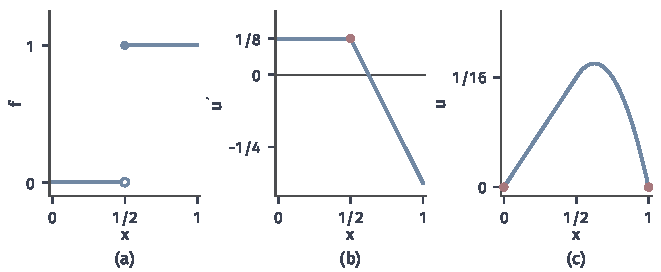
\includegraphics[width=112mm]{figures/06-differential-equations/02-partial-differential-equations/matplotlib/ellip-regularity-ladder/figure.pdf}
  \caption{解比源项多两阶光滑性。(a)源项$f$在$x=1/2$处跳跃。(b)$u'$连续，在红点处有折角。(c)$u$是$C^1$的，曲线在中点看不出异常。由式~\eqref{eq:ellip-interval-solution}，$x\leq1/2$时$u=x/8$，$x\geq1/2$时$u=1/16+(x-\tfrac12)/8-(x-\tfrac12)^2/2$。}
  \label{fig:ellip-regularity-ladder}
\end{BookInlineFigure}

这种增益来自源项，前提是系数足够好。图~\ref{fig:ellip-coefficient-jump}的两段材料中，$f=1$是光滑的，解在界面处却有折角，$u'$有跳跃，$u\notin H^2$。方程能保证的是通量$au'$在$H^1$中，而把$a$除掉后，$u'$的光滑性不会比$a$好。这说明系数必须有一定的光滑性才能得到$H^2$。

\paragraph{为什么Laplace算子能控制全部二阶导数}
多维的情形有一个疑问：方程只给出了$\Delta u$，即二阶导数的一个特定组合，它凭什么控制全部的二阶导数？对$v\in C_c^\infty(\mathbb{R}^{d})$，分部积分两次，
\[
 \int\partial_i\partial_jv\,\partial_i\partial_jv\,\mathrm{d}\bm{x}=\int\partial_i\partial_iv\,\partial_j\partial_jv\,\mathrm{d}\bm{x}.
\]
对$i,j$求和，得到恒等式
\begin{equation}
 \lVert\nabla^2v\rVert_2=\lVert\Delta v\rVert_2 .
 \label{eq:ellip-hessian-identity}
\end{equation}
Hessian的全部元素的平方和，积分后恰好等于$\Delta v$的平方的积分。这个恒等式是椭圆方程内部正则性的核心，其中分部积分需要$v$紧支撑，边界项才能消失。

\paragraph{内部正则性}
定理的形式是：系数Lipschitz，$f\in L^2$，则弱解在内部多一阶导数。我们对$\bm{A}=\bm{I}$完整证明。一般系数的证明思路相同，差商落在系数上会多出一些低阶项，用系数的Lipschitz常数控制，读者可查阅椭圆方程的专著。

\begin{theorem}[内部$H^2$正则性]
\label{thm:ellip-interior}
设$\Omega$是开集，$\bm{A}$一致椭圆且Lipschitz连续，$f\in L^2(\Omega)$，$u\in H^1(\Omega)$满足$a(u,v)=\int_\Omega fv$对所有$v\in C_c^\infty(\Omega)$成立。则对每个$\Omega'$，只要$\overline{\Omega'}$是$\Omega$的紧子集，就有$u\in H^2(\Omega')$，且存在依赖于$\Omega'$和$\bm{A}$的常数$C$，使
\begin{equation}
 \lVert\nabla^2u\rVert_{L^2(\Omega')}\leq C\bigl(\lVert f\rVert_2+\lVert\nabla u\rVert_2\bigr).
 \label{eq:ellip-interior}
\end{equation}
\end{theorem}

注意定理对$u$的边界行为没有任何要求，这是内部正则性的特点。证明的关键技巧是用差商代替导数，因为我们还不知道二阶导数存在，而差商总是存在的。

\begin{proof}[$\bm{A}=\bm{I}$时的证明]
固定方向$\bm{e}_k$，对小的$h\neq0$定义差商
\[
 D^h\phi(\bm{x})=\frac{\phi(\bm{x}+h\bm{e}_k)-\phi(\bm{x})}h .
\]
在下面用到的区域和$h$范围内，有三条性质。

第一，分部求和：若$\phi$或$\psi$紧支撑，$\int(D^h\phi)\psi=-\int\phi\,D^{-h}\psi$。第二，差商不超过导数：设$\phi\in H^1(\Omega)$，$\overline{\Omega''}$是$\Omega$的紧子集，$\lvert h\rvert$小于$\Omega''$到$\partial\Omega$的距离，则由微积分基本定理和Cauchy--Schwarz不等式，
\[
 \lVert D^h\phi\rVert_{L^2(\Omega'')}\leq\lVert\partial_k\phi\rVert_{L^2(\Omega)} .
\]

第三，若$\lVert D^h\phi\rVert_{L^2(\Omega')}$对所有小的$h$有上界$B$，则$\partial_k\phi\in L^2(\Omega')$，且范数不超过$B$。这是因为有界序列$D^{h_n}\phi$有弱收敛子列，把弱极限记为$\Gamma$，对紧支撑的光滑$\psi$有
\[
 \int\Gamma\psi\,\mathrm{d}\bm{x}=-\lim_{n\to\infty}\int\phi\,D^{-h_n}\psi\,\mathrm{d}\bm{x}=-\int\phi\,\partial_k\psi\,\mathrm{d}\bm{x},
\]
所以$\Gamma=\partial_k\phi$。

取$\Omega''$介于$\Omega'$与$\Omega$之间，取截断函数$\eta\in C_c^\infty(\Omega'')$，$0\leq\eta\leq1$，在$\Omega'$上$\eta=1$。记$w=D^hu$，把测试函数取成
\[
 v=-D^{-h}(\eta^2w)\in H^1_0(\Omega) .
\]

由第一条性质，左端变成
\[
 \begin{aligned}
 \int_\Omega\nabla u\cdot\nabla v\,\mathrm{d}\bm{x}&=\int_\Omega\nabla w\cdot\nabla(\eta^2w)\,\mathrm{d}\bm{x}\\
 &=\int_\Omega\eta^2\lVert\nabla w\rVert_2^2\,\mathrm{d}\bm{x}+2\int_\Omega\eta w\,\nabla\eta\cdot\nabla w\,\mathrm{d}\bm{x}.
 \end{aligned}
\]

记$X=\lVert\eta\nabla w\rVert_2$，$B=\lVert w\nabla\eta\rVert_2$。由第二条性质和$0\leq\eta\leq1$，
\[
 \lVert v\rVert_2\leq\lVert\nabla(\eta^2w)\rVert_2\leq X+2B .
\]
$w$的大小也由第二条性质控制，所以$B$不超过$\nabla\eta$的上界与$\lVert\nabla u\rVert_2$的乘积。

把弱形式代入，由Cauchy--Schwarz不等式，得到
\[
 X^2\leq\lVert f\rVert_2(X+2B)+2XB .
\]
用$ab\leq\tfrac14a^2+b^2$吸收含$X$的项，
\[
 \frac12X^2\leq2\lVert f\rVert_2^2+5B^2 .
\]

所以
\[
 \lVert\nabla D^hu\rVert_{L^2(\Omega')}\leq X\leq C\bigl(\lVert f\rVert_2+\lVert\nabla u\rVert_2\bigr),
\]
上界与$h$无关。第三条性质用于每个分量$\partial_ju$，就得到$\partial_k\partial_ju\in L^2(\Omega')$和式~\eqref{eq:ellip-interior}。
\end{proof}

这个结果可以反复使用。$\bm{A}=\bm{I}$时，若$f\in H^1$，$\partial_ku$是源项为$\partial_kf$的弱解，再用一次定理得到$u$在内部属于$H^3$。一般地，$\bm{A}\in C^{k+1}$且$f\in H^k$时，$u$在内部属于$H^{k+2}$。特别地，系数和$f$都光滑时，弱解在内部光滑，调和函数是$C^\infty$的。由Sobolev嵌入，$k>d/2$时$H^k$函数有连续代表，所以$d\leq3$时内部的$H^2$解已经是连续函数。

$L^2$型的增益是整两阶。逐点的情形略有不同，$f$连续不足以保证$u\in C^2$，需要$f$是Hölder连续的。对应的结论称为Schauder估计，证明需要用基本解的奇异积分细致估计，篇幅较长，读者可查阅椭圆方程的专著。其结论是：$\bm{A},f\in C^{0,\gamma}$时$u\in C^{2,\gamma}$在内部成立。

若$\bm{A}$只是有界可测，则没有$H^2$可言，但De Giorgi和Nash的定理仍然给出弱解在内部的Hölder连续性（$f\in L^q$，$q>d/2$），证明同样需要较长的迭代估计，读者可查阅相关专著。

\paragraph{边界正则性}
内部估计依靠截断函数把边界隔开，边界附近没有这个便利，边界的形状成为新的约束。典型的结论如下。

\begin{theorem}[整体$H^2$正则性]
\label{thm:ellip-boundary}
设$\Omega$是有界开集，边界$\partial\Omega$属于$C^{1,1}$，$\bm{A}$在$\overline\Omega$上Lipschitz连续且一致椭圆，$f\in L^2(\Omega)$，$u\in H^1_0(\Omega)$是Dirichlet问题的弱解。则$u\in H^2(\Omega)$，且存在只依赖于$\Omega,\bm{A}$的常数$C$，使
\begin{equation}
 \lVert u\rVert_{H^2(\Omega)}\leq C\lVert f\rVert_2 .
 \label{eq:ellip-boundary-regularity}
\end{equation}
\end{theorem}

证明要把边界局部拉直，篇幅较长，读者可查阅椭圆方程的专著。思路是：拉直后边界是一块平面，沿切向的差商不改变测试函数的零迹，所以内部的论证对切向导数仍然成立，得到除$\partial_{\bm{n}}^2u$之外的二阶导数的估计；剩下的那一个由方程解出，因为方程把它写成了其余二阶导数和$f$的组合。Neumann问题也有类似结论，需要边界数据有相应的光滑性。

$\Omega$是凸多边形且$\bm{A}=\bm{I}$时结论仍成立，并且对零边界的函数有$\lVert\nabla^2u\rVert_2\leq\lVert\Delta u\rVert_2$，证明需要分析边界项的符号，读者可查阅相关专著。但只要边界有向内凹进去的角，结论就失效。

\paragraph{角点}
图~\ref{fig:ellip-corner}的区域是L形，内角$\omega=3\pi/2$的顶点在原点。用极坐标$(r,\theta)$，$\theta\in(0,3\pi/2)$，函数
\begin{equation}
 u=r^{2/3}\sin\frac{2\theta}{3}
 \label{eq:ellip-corner}
\end{equation}
在区域内调和，因为它是复解析函数$z^{2/3}$的虚部，并且在顶点相邻的两条边$\theta=0$、$\theta=3\pi/2$上为零。

\begin{BookInlineFigure}
  \centering
  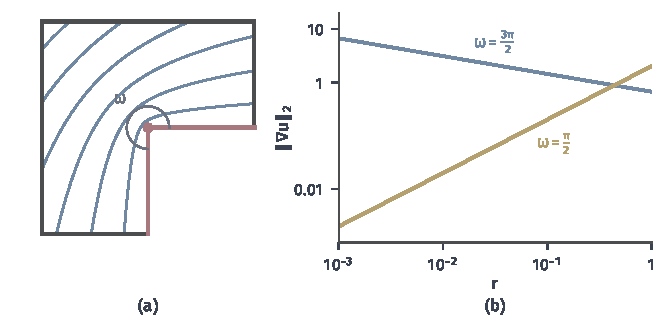
\includegraphics[width=112mm]{figures/06-differential-equations/02-partial-differential-equations/matplotlib/ellip-corner/figure.pdf}
  \caption{角点限制整体光滑性。(a)L形区域上$u=r^{2/3}\sin(2\theta/3)$的等值线，红色的两条边上$u=0$，它们在内角$\omega=3\pi/2$的顶点相交。(b)梯度大小随$r$的变化：$\omega=3\pi/2$时（蓝）$\frac23r^{-1/3}$在顶点爆炸，$\omega=\pi/2$的$r^2\sin2\theta$（黄）梯度$2r$在顶点趋于零。}
  \label{fig:ellip-corner}
\end{BookInlineFigure}

梯度的大小是$\frac23r^{-1/3}$，在顶点处趋于无穷，但其平方可积：
\[
 \int_0^1r^{-2/3}\,r\,\mathrm{d}r<\infty .
\]
所以$u\in H^1$，它是合法的弱解。二阶导数的大小是$r^{-4/3}$量级，平方的积分
\[
 \int_0^1r^{-8/3}\,r\,\mathrm{d}r
\]
发散，所以$u\notin H^2$。再取一个在顶点附近恒为$1$、支撑很小的光滑截断函数$\eta$，令$\tilde u=\eta u$。由乘积法则和$\Delta u=0$，
\[
 -\Delta\tilde u=-2\nabla\eta\cdot\nabla u-u\,\Delta\eta ,
\]
它只在$\eta$不是常数的地方非零，那里$u$光滑。所以$\tilde u$是光滑源项、全零边界值的问题的弱解，在顶点附近却与$u$相同，不属于$H^2$。

一般地，内角$\omega$对应的奇性是$r^{\pi/\omega}$。二阶导数的量级是$r^{\pi/\omega-2}$，平方可积当且仅当$\pi/\omega>1$，即$\omega<\pi$。内角超过$\pi$时奇性无法避免，这不是系数或数据的问题，而是几何本身的限制。

边界条件类型的切换也会产生奇性，哪怕边界本身是光滑的。在上半平面取$u=r^{1/2}\sin(\theta/2)$，它在正半轴$\theta=0$上满足$u=0$，在负半轴$\theta=\pi$上满足$\partial_\theta u=0$。切换点处的梯度量级是$r^{-1/2}$，同样不在$H^2$中。

把各种因素放在一起，可以这样理解：弱解的存在由能量和强制性决定，对光滑性没有要求；更高的光滑性是额外的收获，需要系数、源项和边界几何都配合，其中任何一个粗糙都会限制最终的结果。第~\ref{chap:pde-numerical-methods}章的有限元收敛阶，正是由这里的正则性决定的。


\section{本章小结}
\label{sec:ellip-summary}

开篇的问题是：平衡场的每一点由什么决定？本章的回答是，由整个区域内的源项和整条边界上的数据共同决定，这种全局依赖体现在解的每一种表示之中。

\paragraph{解的结构}
区间上的两次积分展示了最基本的结构：边界贡献和源项贡献线性相加，积分常数由边界条件确定。Green函数把源项的贡献写成点源响应的叠加，$G=\Phi-h$把点源的奇性和边界的修正分开；差分矩阵的逆是它的离散版本。谱展开把算子对角化，$u_k=f_k/\lambda_k$说明解比数据多两阶的光滑性，零特征值则要求先处理核空间。这些公式依赖几何或边界的特殊结构，适用范围有限，也都要求足够的光滑性。

\paragraph{弱理论}
弱形式把一阶导数分给测试函数，让系数跳变和粗糙的源都能进入问题。本质边界条件写进空间，自然边界条件写进积分。Lax--Milgram定理把适定性归结为有界、强制和右端连续三个条件，其证明由Riesz表示和强制性下界完成。三类边界条件的区别，在于怎样处理常数方向，见表~\ref{tab:ellip-summary}。

\begin{BookInlineTable}
  \centering
  \caption{三类边界条件的适定性（$\Omega$有界连通，$\bm{A}$一致椭圆）。}
  \label{tab:ellip-summary}
  \begin{tabular}{lll}
    \toprule
    条件 & 如何排除常数 & 可解性与唯一性\\
    \midrule
    Dirichlet & 零迹与Poincaré不等式 & 任意数据，唯一\\
    Neumann & 零均值子空间 & 需相容条件，差常数\\
    Robin & 边界代价，$\int\beta>0$ & 任意数据，唯一\\
    \bottomrule
  \end{tabular}
\end{BookInlineTable}

\paragraph{三种进一步的结构}
对称问题的弱解是能量的唯一极小点，能量差恰好是误差在能量范数下的平方；非对称问题仍可用Lax--Milgram定理，但没有这种极小刻画。最大值原理依靠符号结构控制逐点的大小，$c\geq0$是必要的结构条件。正则性在内部由系数和源项决定，整体还受边界几何和边界条件切换点的限制。

\paragraph{结论的适用范围}
能量方法和Lax--Milgram定理给出弱解的存在和唯一，对边界和系数的要求很低。最大值原理要求符号条件，经典形式要求解是$C^2$的，弱形式的版本用截断测试函数绕过了这一点。更高的光滑性要求系数、源项和边界同时配合。所有这些结论都是关于平衡场的，没有时间的参与。

第~\ref{chap:diffusion-equations}章在同样的空间和边界模式上引入时间，第~\ref{chap:pde-numerical-methods}章把这里的弱形式在有限维子空间上离散，得到有限元方法。


\chapter{扩散方程}
\label{chap:diffusion-equations}

把一根细铁棒的中段烧热，再放到隔热的架子上。峰顶很快降下去，两侧慢慢热起来，几分钟之后整根棒几乎同样温度。如果把两端插进冰水，结局又不一样：热量不断从两端流走，棒最后回到冰水的温度。这两个过程遵循同一条局部规律，每一点的温度都在向邻居的平均值靠拢，差别只来自端点。

这条规律能回答的问题比“温度怎样变化”更具体。一个任意形状的鼓包，能不能拆成若干互不干扰、各自衰减的形状？如果棒无限长，一点上的热量过了时间$t$散布成什么样子？初始温度有跳跃时，方程在初始时刻是什么意思？持续加热、端点温度随时间变化时，解又怎样写？

具体的解写出来之后，还要问哪些事情不需要公式也能断定：总热量怎样变，最高温能不能升高，温度的起伏被抹平得多快，粗糙的初值过了片刻会变得多光滑。这些估计同时给出唯一性和对数据的连续依赖，而且把条件暴露得很清楚，有界区域上成立的结论，到了无穷远可能失败。

全章以$(0,1)$上的三角形鼓包为贯穿例子。我们先用方程的局部推导和两类端点确定问题，再分别在有界区间和全空间求解，把持续热源和非零边值叠加进来，然后研究质量、极值、能量和光滑性。最后把“从时刻$0$走到时刻$t$”看成一个算子，并反过来问能否由终态恢复初态：向前平滑得越好，向后恢复就越困难。

\section{初边值问题}
\label{sec:heat-ibvp}

取一根长度为$1$的细棒，中点加热到$1/2$度，向两端线性降到$0$度，初始温度就是一个三角形鼓包
\begin{equation}
 u_0(x)=\min\{x,1-x\},\qquad 0\leq x\leq 1 .
 \label{eq:heat-tent}
\end{equation}
棒的侧面包着隔热层，只有两端可能与外界交换热量。松手之后温度怎样变化？回答它需要一个方程，还需要说清初始时刻和两端发生了什么。

\paragraph{局部守恒与Fourier定律}
先看棒上任意一段$[a,b]$。记$u(x,t)$为温度，选取单位，使单位长度的棒升高一度所需的热量为$1$，于是这一段含有的热量是$\int_a^bu\,\mathrm{d}x$。再记$q(x,t)$为单位时间向右穿过截面$x$的热量，$f(x,t)$为单位长度、单位时间内产生的热量。

如图~\ref{fig:heat-bar-balance}，这一段热量的变化只有三个来源：从左端流入，从右端流出，内部产生。写成等式是
\[
 \frac{\mathrm{d}}{\mathrm{d}t}\int_a^bu\,\mathrm{d}x=q(a,t)-q(b,t)+\int_a^bf\,\mathrm{d}x .
\]

\begin{BookInlineFigure}
  \centering
  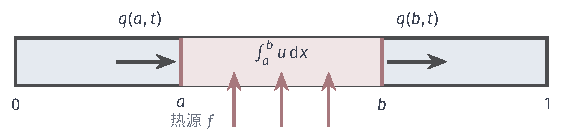
\includegraphics[width=96mm]{figures/06-differential-equations/02-partial-differential-equations/tikz/heat-bar-balance/figure.pdf}
  \caption{细棒上一段$[a,b]$（红色浅底）的热量收支。左右两个箭头是穿过截面的热流$q$，向右为正；下方红色箭头是内部热源$f$。段内热量的变化率等于流入减流出再加内部产生。}
  \label{fig:heat-bar-balance}
\end{BookInlineFigure}

这个等式对任何传递机制都成立，它有$u$和$q$两个未知量，还不能决定演化。补上的一条是物质的性质：热量从高温流向低温，流量正比于温度的斜率，这称为\term{Fourier定律}（Fourier's law）：
\[
 q=-\kappa\,\partial_xu ,
\]
其中$\kappa>0$是导热能力。斜率为正时右边更热，$q<0$，热量向左流，符号正好如此。

设$u$足够光滑。由微积分基本定理，$q(a,t)-q(b,t)=-\int_a^b\partial_xq\,\mathrm{d}x$。把它和Fourier定律代入收支等式，并把对$t$的导数移进积分，得到
\[
 \int_a^b\bigl(\partial_tu-\kappa\,\partial_x^2u-f\bigr)\,\mathrm{d}x=0 .
\]
这对每一段$[a,b]$都成立。被积函数连续，若它在某点不为零，就在一小段上保持同号，取这一小段作$[a,b]$，积分不为零，矛盾。所以被积函数处处为零，即
\begin{equation}
 \partial_tu=\kappa\,\partial_x^2u+f .
 \label{eq:heat-1d-kappa}
\end{equation}
这就是\term{扩散方程}（diffusion equation），在温度的语境下称为\term{热方程}（heat equation）。

\paragraph{向邻居的平均值靠拢}
二阶导数比较的是一点与邻点的平均。由Taylor展开，
\[
 \partial_x^2u(x,t)\approx\frac{2}{h^2}\Bigl(\frac{u(x-h,t)+u(x+h,t)}{2}-u(x,t)\Bigr) .
\]
于是无源时，每一点的温度变化率正比于“邻居平均值减自己”。比邻居平均值高的地方降温，低的地方升温，这就是抹平。

拿式~\eqref{eq:heat-tent}的三角形来看。在两条直线段上，邻居的平均值恰好等于自己，这些点一开始不想变化；只有中点比邻居的平均值高，所以降温从峰顶开始，再逐渐向两侧传开。下面图~\ref{fig:heat-bump-two-boundaries}中最浅的一条曲线正是这样：直线段的大部分还贴着初值，峰顶已经被削圆。

\paragraph{尺度与多维形式}
系数$\kappa$和棒长都可以通过选单位消去。设棒长为$L$，令$x=Ly$、$t=(L^2/\kappa)s$，代入无源方程，得到$\partial_su=\partial_y^2u$。所以时间的自然单位是$L^2/\kappa$：棒长加倍，抹平到同样程度要四倍的时间。这个平方关系后面还会以$\sqrt{t}$的形式反复出现。

高维的推导相同，把截面换成任意小区域的边界，用散度定理把边界通量变成体积分。材料各向异性时通量是$-\bm{A}(\bm{x})\nabla u$，方程是$\partial_tu=\nabla\cdot(\bm{A}\nabla u)+f$，其中$\bm{A}$对称且一致正定。本章取$\bm{A}=\bm{I}$，一维时即$\kappa=1$，这样可以把全部注意力放在解的结构上。

\paragraph{初值、热源与边界}
一个方程不足以确定温度，还要指定开始时的状态和区域边缘的情况。下面把问题写完整，$\Omega\subset\mathbb{R}^{d}$是有界开集，$T>0$。

\begin{definition}[初边值问题]
\label{def:heat-ibvp}
给定源项$f$、初值$u_0$和边界数据$g$，扩散方程的\term{初边值问题}（initial-boundary value problem）是求$u(\bm{x},t)$，使得
\begin{equation}
 \begin{aligned}
  \partial_tu&=\Delta u+f, && \bm{x}\in\Omega,\ 0<t\leq T,\\
  u(\bm{x},0)&=u_0(\bm{x}), && \bm{x}\in\Omega,
 \end{aligned}
 \label{eq:heat-ibvp}
\end{equation}
并在$\partial\Omega\times(0,T]$上满足Dirichlet条件$u=g$或Neumann条件$\partial_{\bm{n}}u=g$。若$\partial_tu$与二阶空间偏导在$\Omega\times(0,T]$上连续，$u$在$\overline\Omega\times[0,T]$上连续，式~\eqref{eq:heat-ibvp}和边界条件逐点成立，就称$u$是\term{经典解}（classical solution）；Neumann情形还要求法向导数在$\partial\Omega\times(0,T]$上存在且连续。
\end{definition}

三种数据各管一件事。初值$u_0$给出出发的状态。方程对时间只有一阶，$\partial_tu$已经由当前的温度分布决定，所以只需要一个初始函数，不必另给初始变化率。源项$f$是持续注入或抽走的热量，$f>0$时加热。边界条件规定外界怎样与区域交换热量。

这些数据在初始时刻的边界上相遇。Dirichlet情形要让$u$在角点连续，必须有$u_0=g(\cdot,0)$，否则解只能在较弱的意义下取得初值；三角形鼓包和零边值满足这一要求。Neumann情形的定义只要求$u$本身连续，式~\eqref{eq:heat-tent}的斜率在端点是$\pm1$，零通量条件要求斜率为$0$，两者不相容，解在角点仍连续，只是空间导数在那里不连续。

\paragraph{固定温度与无通量}
两种齐次边界条件写出来只差一个导数记号，物理含义却完全不同。图~\ref{fig:heat-boundary-meaning}(a)的端点接着大量冰水，温度被钉在$0$，冰水愿意吸收多少热量都可以，通量由解自己决定。图~\ref{fig:heat-boundary-meaning}(b)的端点包着隔热层，通量被规定为零，端点的温度由解自己决定。

\begin{BookInlineFigure}
  \centering
  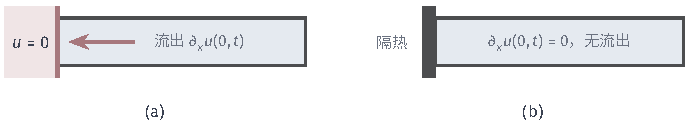
\includegraphics[width=112mm]{figures/06-differential-equations/02-partial-differential-equations/tikz/heat-boundary-meaning/figure.pdf}
  \caption{同一根暖棒左端的两种边界。(a)Dirichlet：端点接冰水，温度固定为$0$，红色箭头表示热量流出，流出率是$\partial_xu(0,t)$，由解决定。(b)Neumann：端点隔热（深灰），通量为零，温度由解决定。}
  \label{fig:heat-boundary-meaning}
\end{BookInlineFigure}

外法向通量是$-\partial_{\bm{n}}u$。所以Neumann数据$\partial_{\bm{n}}u=g>0$表示热量从外面进来，不是流出去。对无源的方程在$(0,1)$上积分，再用微积分基本定理，得到
\[
 \frac{\mathrm{d}}{\mathrm{d}t}\int_0^1u\,\mathrm{d}x=\partial_xu(1,t)-\partial_xu(0,t) .
\]
隔热时右端为零，总热量不变。接冰水时，只要棒内温度为正，左端斜率为正、右端斜率为负，右端小于零，总热量持续减少。

图~\ref{fig:heat-bump-two-boundaries}是同一个三角形在两种边界下的演化，公式下一节推出。短时间内两者几乎一样，因为中段还没有“听到”端点的消息。随后分歧变大：接冰水的鼓包整体下沉到零，隔热的鼓包摊平到平均温度$1/4$。

\begin{BookInlineFigure}
  \centering
  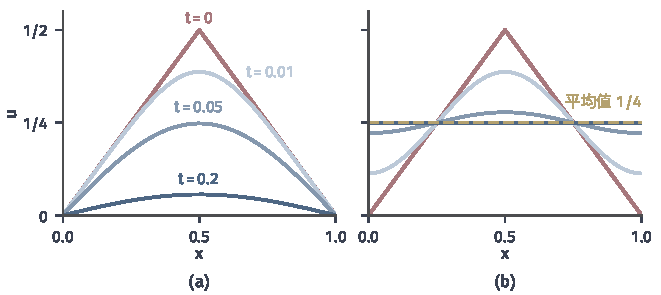
\includegraphics[width=112mm]{figures/06-differential-equations/02-partial-differential-equations/matplotlib/heat-bump-two-boundaries/figure.pdf}
  \caption{三角形初值（红）的演化，蓝色由浅到深为$t=0.01,0.05,0.2$。(a)两端$u=0$。(b)两端$\partial_xu=0$，黄色虚线是初值的平均值$1/4$，$t=0.2$的曲线已与它重合。}
  \label{fig:heat-bump-two-boundaries}
\end{BookInlineFigure}

图~\ref{fig:heat-spacetime-boundaries}把同样的解画在时空平面上。左图的红色竖边表示温度被固定，颜色向上逐渐褪成白色；右图的虚线竖边表示绝热，颜色褪成均匀的浅蓝，总量保留了下来。

\begin{BookInlineFigure}
  \centering
  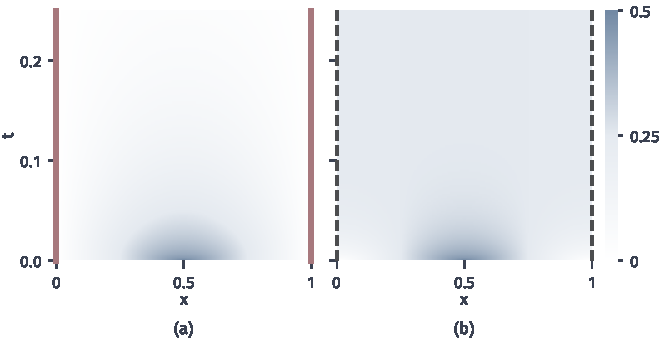
\includegraphics[width=112mm]{figures/06-differential-equations/02-partial-differential-equations/matplotlib/heat-spacetime-boundaries/figure.pdf}
  \caption{三角形初值解的时空温度图，颜色由白到蓝表示温度由$0$到$0.5$，两图色阶相同。(a)两端固定为$0$（红边）。(b)两端无通量（深灰虚边）。}
  \label{fig:heat-spacetime-boundaries}
\end{BookInlineFigure}

把两种条件并列，见表~\ref{tab:heat-boundary-compare}。此外还有介于两者之间的Robin条件$\partial_{\bm{n}}u+\beta u=0$（$\beta>0$），它说流出量正比于端点与环境的温差；$\beta\to0$接近隔热，$\beta\to\infty$接近固定温度。

\begin{BookInlineTable}
  \centering
  \caption{两种齐次边界条件的比较，数值取自三角形初值，$t=0.1$。}
  \label{tab:heat-boundary-compare}
  \begin{tabular}{lll}
    \toprule
    & 固定温度$u=0$ & 无通量$\partial_{\bm{n}}u=0$\\
    \midrule
    规定的量 & 端点温度 & 端点通量\\
    由解决定的量 & 端点通量 & 端点温度\\
    无源时总热量 & 减少 & 不变\\
    $t=0.1$的总热量 & $0.0962$ & $0.2500$\\
    $t=0.1$的中点温度 & $0.1511$ & $0.2539$\\
    \bottomrule
  \end{tabular}
\end{BookInlineTable}


\section{边界模式}
\label{sec:heat-modes}

三角形的形状一直在变，直接跟踪它并不方便。换一个问法：有没有这样的初始形状，演化时形状不变，只是整体按比例缩小？如果有足够多这样的形状，任何初值都可以拆开，各部分分别衰减，再加回去。

\paragraph{离散后的特征向量}
把棒离散成向量，问题就是我们熟悉的。取步长$h=1/4$，内部三个格点$x_j=j/4$，端点取零，用二阶差商代替$\partial_x^2u$，记$\bm{u}(t)$为三个格点上的温度。方程成为线性常微分方程组
\[
 \dot{\bm{u}}=-\bm{K}\bm{u},\qquad
 \bm{K}=16\begin{bmatrix}2&-1&0\\-1&2&-1\\0&-1&2\end{bmatrix} .
\]
矩阵的特征向量正是“形状不变”的初值：若$\bm{K}\bm{v}=\mu\bm{v}$，从$\bm{v}$出发的解是$\mathrm{e}^{-\mu t}\bm{v}$。

三个特征值和特征向量可以手算验证。取$\bm{v}=(\sqrt2/2,\,1,\,\sqrt2/2)^{\top}$，第一行给出$16(\sqrt2-1)\approx6.627$，第二行给出$16(2-\sqrt2)\approx9.373$，比值都是$9.373$，这就是$\mu_1$。全部结果是
\[
 \mu_1=16(2-\sqrt2)\approx9.37,\quad \mu_2=32,\quad \mu_3=16(2+\sqrt2)\approx54.63 .
\]
特征向量恰好是$\sin(k\pi x)$在格点上的取值，$k=1,2,3$，见图~\ref{fig:heat-discrete-modes}。这提示连续问题的“特征向量”是正弦函数，对应的$\mu_k$则应当逼近某个随$k$增长的数。

\begin{BookInlineFigure}
  \centering
  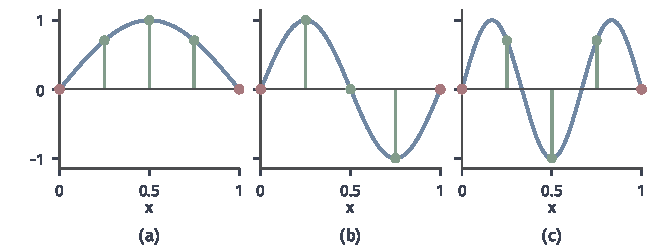
\includegraphics[width=112mm]{figures/06-differential-equations/02-partial-differential-equations/matplotlib/heat-discrete-modes/figure.pdf}
  \caption{三个内部格点的离散问题。绿色竖线是矩阵$\bm{K}$的三个特征向量，蓝线是$\sin(k\pi x)$，红点是固定为零的端点。(a)$k=1$。(b)$k=2$。(c)$k=3$。}
  \label{fig:heat-discrete-modes}
\end{BookInlineFigure}

\paragraph{分离变量}
现在回到连续问题，令$f=0$，寻找形如$u(x,t)=\varphi(x)a(t)$的解，这种做法称为\term{分离变量}（separation of variables）。代入$\partial_tu=\partial_x^2u$，得到
\[
 \varphi(x)\,a'(t)=\varphi''(x)\,a(t) .
\]
在$\varphi$和$a$不为零的地方两边相除，
\[
 \frac{a'(t)}{a(t)}=\frac{\varphi''(x)}{\varphi(x)} .
\]
左边只依赖$t$，右边只依赖$x$，二者相等只能都是常数，记作$-\lambda$。于是偏微分方程分成两个常微分方程：
\begin{equation}
 a'=-\lambda a,\qquad -\varphi''=\lambda\varphi .
 \label{eq:heat-separated}
\end{equation}

时间方程的解是$a(t)=a(0)\mathrm{e}^{-\lambda t}$。空间方程加上边界条件，只对某些$\lambda$有非零解，这称为\term{边界特征值问题}（boundary eigenvalue problem）。边界条件正是在这里进入：它决定哪些形状可用。

\paragraph{Dirichlet边界的模式}
要求$\varphi(0)=\varphi(1)=0$，按$\lambda$的符号分三种情形。

若$\lambda<0$，记$\omega=\sqrt{-\lambda}$，通解是$\varphi=A\cosh\omega x+B\sinh\omega x$。由$\varphi(0)=0$得$A=0$，由$\varphi(1)=B\sinh\omega=0$得$B=0$，没有非零解。

若$\lambda=0$，通解是$\varphi=A+Bx$，两个端点条件同样迫使$A=B=0$。

若$\lambda>0$，记$\omega=\sqrt\lambda$，通解是$\varphi=A\cos\omega x+B\sin\omega x$。由$\varphi(0)=0$得$A=0$。要有非零解，必须$\sin\omega=0$，即$\omega=k\pi$。把振幅归一化后，全部模式是
\begin{equation}
 e_k(x)=\sqrt2\sin(k\pi x),\qquad \lambda_k=k^2\pi^2,\qquad k=1,2,\ldots .
 \label{eq:heat-dirichlet-modes}
\end{equation}

与离散结果比较，连续问题的前三个特征值是
\[
 \lambda_1\approx9.87,\quad \lambda_2\approx39.5,\quad \lambda_3\approx88.8 .
\]
低频的$\mu_1$已经接近$\lambda_1$，高频差别较大，三个格点本来就表示不好高频。

每个模式独立地按$\mathrm{e}^{-k^2\pi^2t}$衰减，频率越高衰减越快。振幅减半的时间是$\ln2/\lambda_k$：$k=1$时约$0.0702$，$k=3$时约$0.0078$，相差九倍。原因就是前面的邻居平均：振荡越快，峰与邻居的落差相对越大。图~\ref{fig:heat-mode-decay}(a)的初值是$\sin(\pi x)+\tfrac12\sin(4\pi x)$，小起伏很快消失，大的拱形缓慢下降；图~\ref{fig:heat-mode-decay}(b)在对数坐标中把衰减画成直线，斜率是$-\lambda_k$。

\begin{BookInlineFigure}
  \centering
  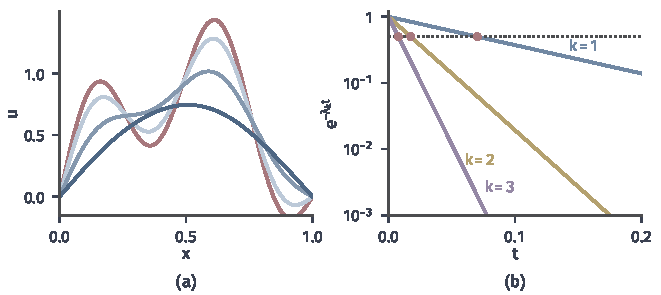
\includegraphics[width=112mm]{figures/06-differential-equations/02-partial-differential-equations/matplotlib/heat-mode-decay/figure.pdf}
  \caption{模式衰减。(a)初值$\sin(\pi x)+\tfrac12\sin(4\pi x)$（红）与$t=0.002,0.008,0.03$的解（蓝色由浅到深）。(b)$k=1,2,3$的振幅因子，纵轴为对数刻度，红点是振幅减半的时刻，虚线高度为$1/2$。}
  \label{fig:heat-mode-decay}
\end{BookInlineFigure}

\paragraph{Neumann边界的模式}
把边界换成$\varphi'(0)=\varphi'(1)=0$，计算只有一处结果不同。$\lambda<0$时，$\varphi'=\omega(A\sinh\omega x+B\cosh\omega x)$，由$\varphi'(0)=0$得$B=0$，由$\varphi'(1)=0$得$A=0$，仍无非零解。$\lambda>0$时，由$\varphi'(0)=0$得$B=0$，再由$\sin\omega=0$得$\omega=k\pi$。

不同的是$\lambda=0$：$\varphi=A+Bx$的导数是$B$，只要$B=0$就满足两个条件，常数活了下来。全部模式是
\begin{equation}
 \tilde{e}_0(x)=1,\quad\lambda_0=0;\qquad \tilde{e}_k(x)=\sqrt2\cos(k\pi x),\quad\lambda_k=k^2\pi^2\quad(k\geq1) .
 \label{eq:heat-neumann-modes}
\end{equation}

$\lambda_0=0$的模式称为\term{零模式}（zero mode），它的时间因子恒为$1$，永远保留。常数没有曲率，每一点都等于邻居的平均值，没有理由变化。这与表~\ref{tab:heat-boundary-compare}的总热量守恒相合：隔热棒里的热量无处可去，它最后全部留在这个常数里。

\paragraph{初值如何确定系数}
要用这些模式表示一般的初值，需要两件事：模式彼此正交，模式足够多。正交性可以直接算。对$j\neq k$，由积化和差，
\[
 \int_0^12\sin(j\pi x)\sin(k\pi x)\,\mathrm{d}x
 =\int_0^1\bigl(\cos((j-k)\pi x)-\cos((j+k)\pi x)\bigr)\,\mathrm{d}x=0 ,
\]
$j=k$时同样的式子给出$1$。

完备性来自Fourier级数：把$(0,1)$上的函数奇延拓到$(-1,1)$，再按周期$2$展开，余弦系数全为零，只剩$\sin(k\pi x)$；偶延拓则只剩余弦。所以$\{e_k\}_{k\geq1}$与$\{\tilde{e}_k\}_{k\geq0}$都是$L^2(0,1)$的标准正交基，三角系统的完备性可参考\BookChapterRef{chap:fourier-transform}{卷四第14章“Fourier变换”}。

于是对$u_0\in L^2(0,1)$，令$c_k=\langle u_0,e_k\rangle$，就有$u_0=\sum_kc_ke_k$（在$L^2$中收敛）和Parseval等式$\sum_kc_k^2=\lVert u_0\rVert_2^2$。把每一项换成衰减后的形式，就得到候选解。它是否真的是解，初值在什么意义下恢复，需要证明。

\begin{theorem}[区间上的模式解]
\label{thm:heat-series}
设$u_0\in L^2(0,1)$，$c_k=\langle u_0,e_k\rangle$，$\lambda_k=k^2\pi^2$，令
\begin{equation}
 u(x,t)=\sum_{k\geq1}c_k\mathrm{e}^{-\lambda_kt}e_k(x) .
 \label{eq:heat-sine-solution}
\end{equation}
则下列结论成立。
\begin{enumerate}
 \item 对每个$t\geq0$，级数在$L^2(0,1)$中收敛，满足
 \begin{equation}
  \lVert u(\cdot,t)\rVert_2\leq\mathrm{e}^{-\pi^2t}\lVert u_0\rVert_2,
  \label{eq:heat-series-decay}
 \end{equation}
 并且$t\to0^+$时$\lVert u(\cdot,t)-u_0\rVert_2\to0$。
 \item 级数及其任意阶逐项导数在$[0,1]\times[t_0,\infty)$上一致收敛（$t_0>0$），所以$u$在$[0,1]\times(0,\infty)$上无穷次可微，逐点满足热方程和零边值。
 \item 若$u_0$连续、分段连续可微且$u_0(0)=u_0(1)=0$，则$\sum_k\lvert c_k\rvert<\infty$，$u$在$[0,1]\times[0,\infty)$上连续，$u(\cdot,0)=u_0$处处成立，$u$是定义~\ref{def:heat-ibvp}意义下的经典解。
\end{enumerate}
\end{theorem}

\begin{proof}
(1)由Parseval等式，系数$c_k\mathrm{e}^{-\lambda_kt}$平方可和，级数收敛。又$\lambda_k\geq\pi^2$，所以
\[
 \lVert u(\cdot,t)\rVert_2^2=\sum_kc_k^2\mathrm{e}^{-2\lambda_kt}\leq\mathrm{e}^{-2\pi^2t}\sum_kc_k^2 .
\]
这就是式~\eqref{eq:heat-series-decay}。初值的恢复同样按坐标计算：
\[
 \lVert u(\cdot,t)-u_0\rVert_2^2=\sum_kc_k^2\bigl(1-\mathrm{e}^{-\lambda_kt}\bigr)^2 .
\]
每一项在$t\to0^+$时趋于零，且不超过可和的$c_k^2$，由级数的控制收敛定理，和趋于零。

(2)由Parseval等式，$\lvert c_k\rvert\leq\lVert u_0\rVert_2$。对$x$求$m$次、对$t$求$n$次后，第$k$项在$t\geq t_0$上的绝对值不超过
\[
 \sqrt2\,\lVert u_0\rVert_2\,(k\pi)^{m+2n}\,\mathrm{e}^{-k^2\pi^2t_0} .
\]
指数因子比$k$的任何幂衰减得都快，这个上界关于$k$可和。由Weierstrass判别法，各阶导数的级数一致收敛，可以逐项求导。每一项都满足方程和零边值，极限也满足。

(3)分部积分一次，边界项因$u_0$在端点为零而消失，得到
\[
 c_k=\frac{1}{k\pi}\int_0^1u_0'(x)\,\sqrt2\cos(k\pi x)\,\mathrm{d}x=\frac{b_k}{k\pi},
\]
其中$b_k$是$u_0'$在标准正交系$\sqrt2\cos(k\pi x)$上的坐标，由Bessel不等式$\sum_kb_k^2\leq\lVert u_0'\rVert_2^2$。再由Cauchy--Schwarz不等式和$\sum_kk^{-2}=\pi^2/6$，
\[
 \sum_k\lvert c_k\rvert\leq\Bigl(\sum_k\frac{1}{k^2\pi^2}\Bigr)^{1/2}\Bigl(\sum_kb_k^2\Bigr)^{1/2}\leq\frac{\lVert u_0'\rVert_2}{\sqrt6} .
\]
于是级数的第$k$项被$\sqrt2\lvert c_k\rvert$一致控制，$u$是连续函数的一致极限，在$[0,1]\times[0,\infty)$上连续。$t=0$时$u(\cdot,0)$连续，又在$L^2$中等于$u_0$，两个连续函数几乎处处相等就处处相等。
\end{proof}

定理的三条分别回答三个问题。第一条对最粗糙的数据也成立，但只说平方积分的距离趋于零，不说每一点的值。第二条说只要过了一点时间，解就无穷光滑，初值有多粗糙无关紧要。第三条说初值和边界相容且有一点光滑性时，一致地恢复。

\begin{example}[三角形的系数]
\label{ex:heat-tent-coefficients}
取式~\eqref{eq:heat-tent}的$u_0$。它连续、分段线性、两端为零，定理~\ref{thm:heat-series}的第三条适用。在$(0,1/2)$上$u_0'=1$，在$(1/2,1)$上$u_0'=-1$，所以
\[
 \int_0^1u_0\sin(k\pi x)\,\mathrm{d}x
 =\frac{1}{k\pi}\Bigl(\int_0^{1/2}\cos(k\pi x)\,\mathrm{d}x-\int_{1/2}^1\cos(k\pi x)\,\mathrm{d}x\Bigr) .
\]
计算两个积分，每一个都贡献$\sin(k\pi/2)/(k\pi)$，于是
\[
 c_k=\frac{2\sqrt2\,\sin(k\pi/2)}{k^2\pi^2} .
\]
偶数$k$的系数为零，这是因为三角形关于中点对称，偶数模式关于中点反对称。前三个非零系数是
\[
 c_1\approx0.2866,\quad c_3\approx-0.0318,\quad c_5\approx0.0115 .
\]
代入式~\eqref{eq:heat-sine-solution}，解是
\[
 u(x,t)=\sum_{k\text{ 奇}}\frac{4\sin(k\pi/2)}{k^2\pi^2}\,\mathrm{e}^{-k^2\pi^2t}\sin(k\pi x) .
\]
\end{example}

在中点，$\sin^2(k\pi/2)=1$，只取第一项得到$\tfrac{4}{\pi^2}\mathrm{e}^{-\pi^2t}$。表~\ref{tab:heat-tent-center}把它与多项求和的结果比较。$t=0$时第一项差得很远，$t=0.1$时已经精确到小数点后三位以上，因为高频项衰减得太快。

\begin{BookInlineTable}
  \centering
  \caption{三角形初值的中点温度$u(1/2,t)$：只取$k=1$一项与级数求和的比较。}
  \label{tab:heat-tent-center}
  \begin{tabular}{lllllll}
    \toprule
    $t$ & $0$ & $0.01$ & $0.02$ & $0.05$ & $0.1$ & $0.2$\\
    \midrule
    第一项 & $0.4053$ & $0.3672$ & $0.3327$ & $0.2474$ & $0.1511$ & $0.0563$\\
    级数 & $0.5000$ & $0.3872$ & $0.3404$ & $0.2480$ & $0.1511$ & $0.0563$\\
    \bottomrule
  \end{tabular}
\end{BookInlineTable}

图~\ref{fig:heat-tent-series}显示了同一件事。图(a)中，$t=0$的系数按$k^{-2}$缓慢下降，时间稍一增加，高频系数就断崖式跌落。图(b)中，初值的折角需要很多项才能描出来；图(c)中，$t=0.02$时一项就很接近真解了。

\begin{BookInlineFigure}
  \centering
  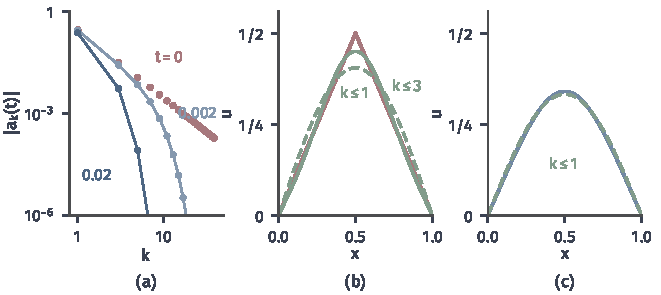
\includegraphics[width=112mm]{figures/06-differential-equations/02-partial-differential-equations/matplotlib/heat-tent-series/figure.pdf}
  \caption{三角形初值的正弦展开。(a)奇数$k$上系数的绝对值$\lvert a_k(t)\rvert=\lvert c_k\rvert\mathrm{e}^{-\lambda_kt}$，红点$t=0$，蓝色点线$t=0.002,0.02$。(b)$t=0$：三角形（红）与$k\leq1$（绿色虚线）、$k\leq3$（绿色实线）的部分和。(c)$t=0.02$：真解（蓝）与$k\leq1$的部分和（绿色虚线）。}
  \label{fig:heat-tent-series}
\end{BookInlineFigure}

\paragraph{Neumann问题与平均值}
余弦基的情形把上面的论证逐字重复，只需注意$\lambda_0=0$。设$u_0\in L^2(0,1)$，$a_0=\int_0^1u_0\,\mathrm{d}x$，$a_k=\langle u_0,\tilde{e}_k\rangle$，解是
\begin{equation}
 u(x,t)=a_0+\sum_{k\geq1}a_k\mathrm{e}^{-k^2\pi^2t}\tilde{e}_k(x) .
 \label{eq:heat-cosine-solution}
\end{equation}
同样的Parseval计算给出
\[
 \lVert u(\cdot,t)-a_0\rVert_2\leq\mathrm{e}^{-\pi^2t}\lVert u_0-a_0\rVert_2 ,
\]
所以温度趋于初值的平均值。

对三角形，$a_0=1/4$。分部积分一次，$\int_0^1u_0\cos(k\pi x)\,\mathrm{d}x$等于$\bigl(2\cos(k\pi/2)-1-(-1)^k\bigr)/(k^2\pi^2)$。只有$k\equiv2\pmod4$时它不为零，等于$-4/(k^2\pi^2)$，于是
\[
 u(x,t)=\frac14-\sum_{k\equiv2\ (\mathrm{mod}\ 4)}\frac{8}{k^2\pi^2}\,\mathrm{e}^{-k^2\pi^2t}\cos(k\pi x) .
\]
最慢的非常数项是$k=2$，衰减率$4\pi^2$，比一般的上界$\pi^2$快。原因仍是对称：$\cos\pi x$关于中点反对称，三角形不含这一分量。例如$t=0.1$时，$\tfrac{2}{\pi^2}\mathrm{e}^{-0.4\pi^2}\approx0.0039$，所以中点温度约$0.2539$，端点温度约$0.2461$，与图~\ref{fig:heat-zero-mode}(a)一致。

\begin{BookInlineFigure}
  \centering
  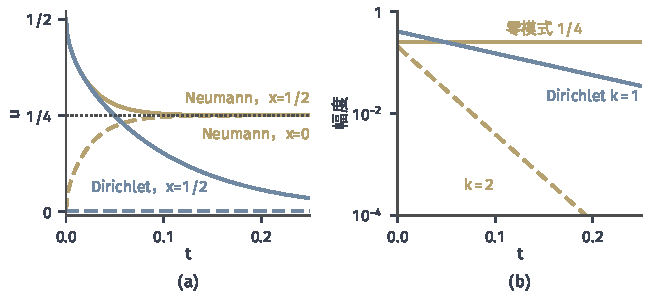
\includegraphics[width=112mm]{figures/06-differential-equations/02-partial-differential-equations/matplotlib/heat-zero-mode/figure.pdf}
  \caption{三角形初值下零模式的作用。(a)中点（实线）与端点（虚线）的温度：Neumann（黄）两条线都趋于$1/4$，Dirichlet（蓝）趋于$0$，蓝色虚线是固定为零的端点。(b)模式幅度，纵轴为对数：Neumann的常数模式$1/4$（黄实线）不变，$k=2$模式幅度$2\pi^{-2}\mathrm{e}^{-4\pi^2t}$（黄虚线）；Dirichlet最低模式幅度$4\pi^{-2}\mathrm{e}^{-\pi^2t}$（蓝）。}
  \label{fig:heat-zero-mode}
\end{BookInlineFigure}

\paragraph{不相容的初值}
定理~\ref{thm:heat-series}第一条的“$L^2$意义下”不是多余的谨慎。取$u_0=1$，两端仍固定为零，初值和边值在角点矛盾。系数是$c_k=\sqrt2(1-(-1)^k)/(k\pi)$，奇数项上为$2\sqrt2/(k\pi)$，于是$\sum_k\lvert c_k\rvert=\infty$，定理的第三条不能用。

$t=0$时部分和在$L^2$中收敛到$1$，但每个部分和在端点都等于$0$，而且靠近端点有固定幅度的过冲，这是\term{Gibbs现象}（Gibbs phenomenon）：奇延拓在端点有高度为$2$的跳跃，部分和的最大值趋于约$1.179$，取$k\leq61$时算得的最大值就是这个数，如图~\ref{fig:heat-corner-layer}(a)。

$t>0$时情形完全改变。定理第二条保证解光滑并且在端点为零，温度在边界附近形成一层过渡，图~\ref{fig:heat-corner-layer}(b)。层的厚度由$\sqrt{t}$决定：把横轴换成$x/(2\sqrt{t})$，不同时刻的层重合到同一条曲线，图~\ref{fig:heat-corner-layer}(c)，这条曲线的公式在下一节得到。

\begin{BookInlineFigure}
  \centering
  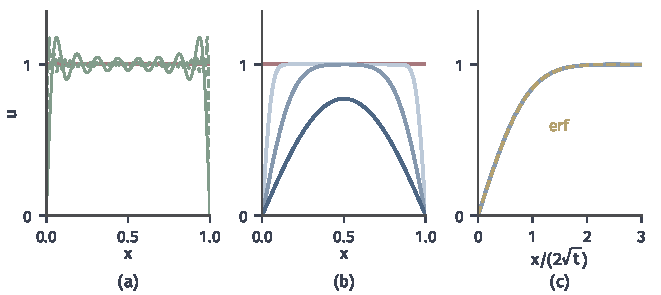
\includegraphics[width=112mm]{figures/06-differential-equations/02-partial-differential-equations/matplotlib/heat-corner-layer/figure.pdf}
  \caption{初值$u_0=1$与零边值不相容。(a)$t=0$：$k\leq15$（绿实线）与$k\leq61$（绿虚线）的部分和在红线附近振荡，端点旁有不随项数消失的过冲。(b)$t=0.001,0.01,0.05$的解（蓝色由浅到深），没有振荡。(c)$t=0.001$、$0.01$的边界层换成变量$x/(2\sqrt{t})$后重合，黄色虚线是$\operatorname{erf}$。}
  \label{fig:heat-corner-layer}
\end{BookInlineFigure}

于是，初值在什么意义下恢复取决于数据：一般的$L^2$初值在$L^2$意义下恢复；连续、分段可微且与边界相容的初值一致地恢复；与边界矛盾的初值在角点附近不可能一致地恢复，但这不妨碍$t>0$时的解是光滑的。


\section{热核}
\label{sec:heat-kernel}

棒无限长时没有端点来挑选模式，频率不再是离散的$k\pi$，而是连成一片。此时局部的一点热量怎样影响后来的场？我们考虑全空间的问题
\begin{equation}
 \partial_tu=\Delta u,\quad \bm{x}\in\mathbb{R}^{d},\ t>0;\qquad u(\bm{x},0)=u_0(\bm{x}) .
 \label{eq:heat-cauchy}
\end{equation}
先用Fourier变换形式地求出公式，再撇开形式推导，直接检验公式在什么条件下给出解、在什么意义下取回初值。

\subsection{核的构造}
\label{sec:heat-kernel-construction}

\paragraph{每个频率一个标量方程}
沿用卷四的约定，Fourier变换写成
\[
 \widehat{u}(\bm{\xi})=\int u(\bm{x})\mathrm{e}^{-2\pi\mathrm{i}\bm{x}\cdot\bm{\xi}}\,\mathrm{d}\bm{x} .
\]
这时对$x_j$求导对应乘以$2\pi\mathrm{i}\xi_j$，Laplace算子对应乘以$-4\pi^2\lvert\bm{\xi}\rvert^2$，这些运算规则都在上一节所引的卷四一章中建立。

设$u$足够好，对式~\eqref{eq:heat-cauchy}关于$\bm{x}$作变换。偏微分方程对每个固定的$\bm{\xi}$变成一个标量常微分方程：
\[
 \partial_t\widehat{u}(\bm{\xi},t)=-4\pi^2\lvert\bm{\xi}\rvert^2\,\widehat{u}(\bm{\xi},t) .
\]
这与上一节的$a'=-\lambda a$完全相同，只是$\lambda$换成了连续变化的$4\pi^2\lvert\bm{\xi}\rvert^2$。解出来是
\begin{equation}
 \widehat{u}(\bm{\xi},t)=\mathrm{e}^{-4\pi^2\lvert\bm{\xi}\rvert^2t}\,\widehat{u}_0(\bm{\xi}) .
 \label{eq:heat-fourier-solution}
\end{equation}
两种模式的对应是精确的：$\sin(k\pi x)=\sin(2\pi(k/2)x)$的频率是$\xi=k/2$，代入$4\pi^2\xi^2$恰好得到$k^2\pi^2$。

\paragraph{乘法还原为卷积}
频域的乘积对应空间的卷积，所以只需找到一个函数，它的变换是$\mathrm{e}^{-4\pi^2\lvert\bm{\xi}\rvert^2t}$。卷四已经算过：$\mathrm{e}^{-\pi\lvert\bm{x}\rvert^2}$的变换是它自身；又把函数$g(\bm{x})$换成$s^{-d}g(\bm{x}/s)$，变换从$\widehat{g}(\bm{\xi})$变成$\widehat{g}(s\bm{\xi})$。

要让指数对上，需要$\pi s^2=4\pi^2t$，即$s=\sqrt{4\pi t}$，这样就得到下面的函数。

\begin{definition}[热核]
\label{def:heat-kernel}
$\mathbb{R}^{d}$上的\term{热核}（heat kernel）是
\begin{equation}
 G(\bm{x},t)=\frac{1}{(4\pi t)^{d/2}}\exp\Bigl(-\frac{\lvert\bm{x}\rvert^2}{4t}\Bigr),\qquad \bm{x}\in\mathbb{R}^{d},\ t>0 .
 \label{eq:heat-kernel}
\end{equation}
对初值$u_0$，定义\term{卷积表示}（convolution representation）
\begin{equation}
 u(\bm{x},t)=\int_{\mathbb{R}^{d}}G(\bm{x}-\bm{y},t)\,u_0(\bm{y})\,\mathrm{d}\bm{y} .
 \label{eq:heat-convolution}
\end{equation}
\end{definition}

到这里的推导要求$u$有变换、能逐点解常微分方程、乘积能还原，都是形式的。下面的做法不再依赖它们，而是直接研究式~\eqref{eq:heat-kernel}和式~\eqref{eq:heat-convolution}。

\begin{theorem}[热核的基本性质]
\label{thm:heat-kernel-properties}
对$t>0$，式~\eqref{eq:heat-kernel}的$G$满足：
\begin{enumerate}
 \item $G>0$，并且$G(\cdot,t)$在$\mathbb{R}^{d}$上的积分等于$1$；
 \item 满足尺度关系
 \begin{equation}
  G(\bm{x},t)=t^{-d/2}G(\bm{x}/\sqrt{t},1) ;
  \label{eq:heat-kernel-scaling}
 \end{equation}
 \item 每个坐标的二阶矩等于$2t$；
 \item 在$\mathbb{R}^{d}\times(0,\infty)$上$\partial_tG=\Delta G$。
\end{enumerate}
\end{theorem}

\begin{proof}
正性由公式可见。积分按坐标分解成$d$个一维积分的乘积。一维情形代换$x=2\sqrt{t}\,z$，
\[
 \int_{\mathbb{R}}\frac{1}{\sqrt{4\pi t}}\mathrm{e}^{-x^2/(4t)}\,\mathrm{d}x=\frac{1}{\sqrt\pi}\int_{\mathbb{R}}\mathrm{e}^{-z^2}\,\mathrm{d}z=1 .
\]
尺度关系由公式直接代入得到。二阶矩中其余坐标积分为$1$，剩下的一维积分用同一代换，再用$\int z^2\mathrm{e}^{-z^2}\,\mathrm{d}z=\sqrt\pi/2$，得到
\[
 \int_{\mathbb{R}}x^2G(x,t)\,\mathrm{d}x=\frac{4t}{\sqrt\pi}\int_{\mathbb{R}}z^2\mathrm{e}^{-z^2}\,\mathrm{d}z=2t .
\]

最后计算导数。令$r=\lvert\bm{x}\rvert$，对$t$求导得到
\[
 \partial_tG=\Bigl(-\frac{d}{2t}+\frac{r^2}{4t^2}\Bigr)G .
\]
对$x_i$求一次导数得$\partial_iG=-\tfrac{x_i}{2t}G$，再求一次并对$i$求和，
\[
 \Delta G=\sum_{i}\Bigl(-\frac{1}{2t}+\frac{x_i^2}{4t^2}\Bigr)G=\Bigl(-\frac{d}{2t}+\frac{r^2}{4t^2}\Bigr)G .
\]
两式相等。
\end{proof}

四条性质各有含义。正性和积分为$1$说卷积是一种加权平均，总热量不变。尺度关系说时间不产生新形状，只把同一个钟形按$\sqrt{t}$拉宽、按$t^{-d/2}$压低。二阶矩说方差随时间线性增长，所以宽度是$\sqrt{2t}$。

具体地，一维时$t=0.01,0.04,0.16$的峰值是$2.82,\,1.41,\,0.705$，标准差是$0.141,\,0.283,\,0.566$：时间变为四倍，宽度加倍，峰值减半，图~\ref{fig:heat-kernel-scaling}。这就是初边值问题里“棒长加倍、时间四倍”的另一面。

\begin{BookInlineFigure}
  \centering
  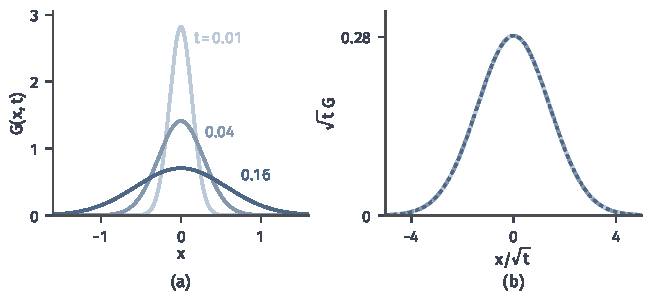
\includegraphics[width=112mm]{figures/06-differential-equations/02-partial-differential-equations/matplotlib/heat-kernel-scaling/figure.pdf}
  \caption{一维热核。(a)$t=0.01,0.04,0.16$时的$G(x,t)$（蓝色由浅到深）。(b)改用尺度化坐标后的$\sqrt{t}\,G$与$x/\sqrt{t}$，三个时刻（实线、虚线、点线）重合到同一条曲线。}
  \label{fig:heat-kernel-scaling}
\end{BookInlineFigure}

\paragraph{卷积是加权平均}
式~\eqref{eq:heat-convolution}的读法是：时刻$t$在$\bm{x}$处的温度，是初值以$\bm{x}$为中心、宽度约$\sqrt{2t}$的Gauss加权平均。也可以反过来读：$\bm{y}$处的一点初始热量$u_0(\bm{y})\,\mathrm{d}\bm{y}$，到时刻$t$散成以$\bm{y}$为中心的钟形，所有钟形叠加成解。

取方框$u_0=\mathbb{I}_{[-1/2,1/2]}$为例。引入误差函数
\[
 \operatorname{erf}(z)=\frac{2}{\sqrt\pi}\int_0^z\mathrm{e}^{-s^2}\,\mathrm{d}s .
\]
一维积分经代换$z=(x-y)/(2\sqrt{t})$化为
\begin{equation}
 u(x,t)=\frac12\Bigl(\operatorname{erf}\frac{x+1/2}{2\sqrt{t}}-\operatorname{erf}\frac{x-1/2}{2\sqrt{t}}\Bigr) .
 \label{eq:heat-box-solution}
\end{equation}

图~\ref{fig:heat-convolution-weights}取$x=0.7$，$t=0.04$。紫色钟形在方框内的部分（蓝色浅底）的面积就是这一点的温度，代入式~\eqref{eq:heat-box-solution}得$0.240$。这一点在方框外，初值为零，可是加权平均已经够到了方框。

\begin{BookInlineFigure}
  \centering
  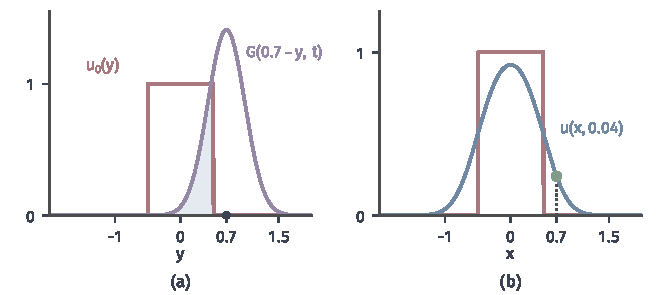
\includegraphics[width=112mm]{figures/06-differential-equations/02-partial-differential-equations/matplotlib/heat-convolution-weights/figure.pdf}
  \caption{卷积作为加权平均。(a)方框初值（红）与以$x=0.7$为中心、$t=0.04$的权重$G(0.7-y,t)$（紫），蓝色浅底的面积等于$u(0.7,0.04)$。(b)解$u(\cdot,0.04)$（蓝），绿点是$x=0.7$处的值$0.240$。}
  \label{fig:heat-convolution-weights}
\end{BookInlineFigure}

\paragraph{传播范围}
热核处处为正，于是只要$u_0\geq0$不恒为零，对任意小的$t>0$，$u$在每一点都严格为正。扰动瞬间到达无穷远，这一性质称为\term{无穷传播速度}（infinite speed of propagation），它与下一章波动方程的有限速度截然不同。

但“到达”的量极小。由式~\eqref{eq:heat-box-solution}，$t=0.01$时距离方框中心$2$的地方温度只有约$1.4\times10^{-26}$，$t=0.1$时距离$3$的地方约$1.1\times10^{-8}$。图~\ref{fig:heat-tails}(a)中尾部在对数坐标下是向下弯的抛物线，这是$\mathrm{e}^{-x^2/(4t)}$的特征。

想知道“热量实际传到哪里”，可以固定一个小的阈值看等值线。图~\ref{fig:heat-tails}(b)是$u=10^{-3}$的位置，它按$\sqrt{t}$前进，早期很快，后来越来越慢，并不是匀速推进的波前。

\begin{BookInlineFigure}
  \centering
  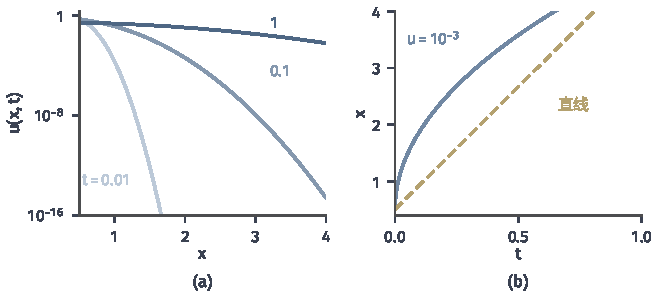
\includegraphics[width=112mm]{figures/06-differential-equations/02-partial-differential-equations/matplotlib/heat-tails/figure.pdf}
  \caption{方框初值的远场。(a)$x>1/2$上的解，纵轴对数，$t=0.01,0.1,1$（蓝色由浅到深）。(b)等值线$u=10^{-3}$的位置（蓝），黄色虚线是连接其起点和终点的直线，匀速前进的前沿应当沿这样的直线。}
  \label{fig:heat-tails}
\end{BookInlineFigure}

这里要说清类比的边界。把热核读成“热量瞬间传到远处”，描述的是这个数学模型。真实的热传递由有限速度的微观运动实现，Fourier定律只是在足够大的尺度上的近似，远处$10^{-26}$量级的温度变化没有物理意义。模型的价值在于$\sqrt{t}$的尺度和被压到极小的尾部，而不在严格的正性上。

\paragraph{频率的衰减}
同一个解也可以在频域读。式~\eqref{eq:heat-fourier-solution}说，频率$\bm{\xi}$的分量乘以$\mathrm{e}^{-4\pi^2\lvert\bm{\xi}\rvert^2t}$。这个因子在$\lvert\bm{\xi}\rvert=1/(2\pi\sqrt{t})$处降到$\mathrm{e}^{-1}$，更高的频率几乎全被抹掉。例如$t=0.01$时$\xi=5$的因子是$\mathrm{e}^{-\pi^2}\approx5\times10^{-5}$。

所以热核是一个低通滤波器，时间越长，通带越窄，图~\ref{fig:heat-fourier-multiplier}。空间和频率的两种读法互为对偶：空间上钟形的宽度按$\sqrt{t}$增长，频率上通带的宽度按$1/\sqrt{t}$收缩。方框的尖角含有缓慢衰减的高频，滤掉之后角就圆了。

\begin{BookInlineFigure}
  \centering
  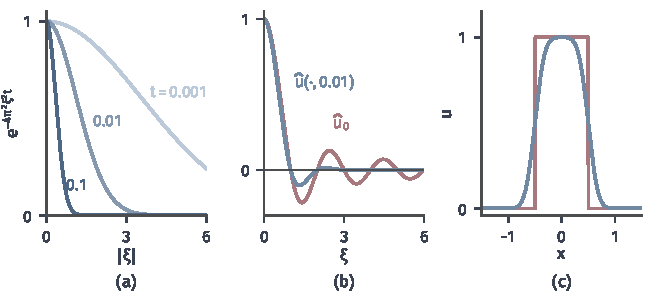
\includegraphics[width=112mm]{figures/06-differential-equations/02-partial-differential-equations/matplotlib/heat-fourier-multiplier/figure.pdf}
  \caption{热传播的频域作用。(a)乘子$\mathrm{e}^{-4\pi^2\xi^2t}$，$t=0.001,0.01,0.1$（蓝色由浅到深）。(b)方框的变换$\widehat{u}_0=\sin(\pi\xi)/(\pi\xi)$（红）与乘上$t=0.01$的乘子后的结果（蓝）。(c)空间中的方框（红）与$t=0.01$的解（蓝）。}
  \label{fig:heat-fourier-multiplier}
\end{BookInlineFigure}

\paragraph{公式何时给出解}
式~\eqref{eq:heat-convolution}的积分未必收敛。$u_0$可以无界，但不能增长得比核衰减得还快。下面的条件恰好刻画这个界线：存在$T>0$，使
\begin{equation}
 \int_{\mathbb{R}^{d}}\lvert u_0(\bm{y})\rvert\,\mathrm{e}^{-\lvert\bm{y}\rvert^2/(4T)}\,\mathrm{d}\bm{y}<\infty .
 \label{eq:heat-integrability}
\end{equation}
有界的可测函数、$L^p$函数（$1\leq p\leq\infty$）都满足它，并且$T$可以取任意正数。

\begin{theorem}[卷积解的可微性]
\label{thm:heat-convolution-smooth}
设$u_0$可测且满足式~\eqref{eq:heat-integrability}。则式~\eqref{eq:heat-convolution}的积分对$\bm{x}\in\mathbb{R}^{d}$、$0<t<T$绝对收敛，$u$在$\mathbb{R}^{d}\times(0,T)$上无穷次可微，且可以在积分号下求导；特别地
\begin{equation}
 \partial_tu=\Delta u,\qquad \bm{x}\in\mathbb{R}^{d},\ 0<t<T .
 \label{eq:heat-convolution-solves}
\end{equation}
\end{theorem}

\begin{proof}
固定紧集$K\subset\mathbb{R}^{d}\times(0,T)$，其上$\lvert\bm{x}\rvert\leq R$，$t_0\leq t\leq t_1<T$。关键是用一个与$(\bm{x},t)$无关的可积函数控制被积函数及其导数。

取$\theta>0$使$(1+\theta)t_1<T$，再取$\sigma\in(0,1)$，使$(1+\theta)t_1/(1-\sigma)\leq T$。由三角不等式和Young不等式，对任意$\bm{x},\bm{y}$，
\[
 \lvert\bm{y}\rvert^2\leq(1+\theta)\lvert\bm{x}-\bm{y}\rvert^2+\bigl(1+\theta^{-1}\bigr)\lvert\bm{x}\rvert^2 .
\]
把它改写成对$\lvert\bm{x}-\bm{y}\rvert^2$的下界，并用$t\leq t_1$，得到
\[
 \frac{(1-\sigma)\lvert\bm{x}-\bm{y}\rvert^2}{4t}\geq\frac{(1-\sigma)\lvert\bm{y}\rvert^2}{4(1+\theta)t_1}-C_1\geq\frac{\lvert\bm{y}\rvert^2}{4T}-C_1 ,
\]
其中常数$C_1$只依赖$R$、$t_0$、$\theta$、$\sigma$。

$G$对$\bm{x}$、$t$的任意阶导数等于$G$乘以一个$\bm{x}$和$1/t$的多项式。在$K$上这个多项式关于$\lvert\bm{x}-\bm{y}\rvert$有多项式增长，而多项式被指数$\mathrm{e}^{-\sigma\lvert\bm{x}-\bm{y}\rvert^2/(4t)}$压住。于是每个导数的绝对值满足
\[
 \bigl\lvert\partial^{\alpha}_{\bm{x}}\partial_t^{n}G(\bm{x}-\bm{y},t)\bigr\rvert\leq C\,\mathrm{e}^{-(1-\sigma)\lvert\bm{x}-\bm{y}\rvert^2/(4t)}\leq C'\,\mathrm{e}^{-\lvert\bm{y}\rvert^2/(4T)} .
\]
乘以$\lvert u_0\rvert$后可积。由控制收敛定理，积分绝对收敛，且可以在积分号下任意次求导。定理~\ref{thm:heat-kernel-properties}的第四条给出式~\eqref{eq:heat-convolution-solves}。
\end{proof}

这个结论里没有要求初值连续，这是扩散的平滑作用的第一次定量出现，后面还要专门研究。条件中的$T$不能随意增大，下面的例子说明它是准确的。

\begin{example}[快速增长的初值]
\label{ex:heat-gaussian-growth}
取$d=1$，$u_0(x)=\mathrm{e}^{ax^2}$，$a>0$。此时式~\eqref{eq:heat-integrability}成立当且仅当$T<1/(4a)$。式~\eqref{eq:heat-convolution}的指数是$y$的二次式，记$p=1/(4t)-a$，当$t<1/(4a)$时$p>0$。把指数写成
\[
 -py^2+\frac{xy}{2t}-\frac{x^2}{4t} .
\]
由Gauss积分
\[
 \int_{\mathbb{R}}\mathrm{e}^{-py^2+by}\,\mathrm{d}y=\sqrt{\frac{\pi}{p}}\,\mathrm{e}^{b^2/(4p)},
\]
取$b=x/(2t)$，振幅因子是$(4\pi t)^{-1/2}\sqrt{\pi/p}$，它等于$(1-4at)^{-1/2}$。指数部分合并后是$ax^2/(1-4at)$，于是
\begin{equation}
 u(x,t)=\frac{1}{\sqrt{1-4at}}\exp\Bigl(\frac{ax^2}{1-4at}\Bigr),\qquad 0\leq t<\frac{1}{4a} .
 \label{eq:heat-gaussian-growth}
\end{equation}
$t\to1/(4a)$时$u(0,t)\to\infty$，解在有限时间爆炸。
\end{example}

图~\ref{fig:heat-growth-limit}取$a=1/2$，由式~\eqref{eq:heat-gaussian-growth}，爆炸时刻是$t=1/2$。这里的爆炸并不违背“热量被抹平”的直觉：无穷远处温度增长得太快，加权平均从远处吸进来的热量越来越多，直到积分发散。

\begin{BookInlineFigure}
  \centering
  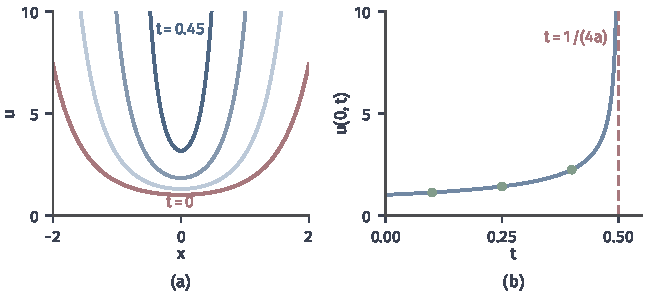
\includegraphics[width=112mm]{figures/06-differential-equations/02-partial-differential-equations/matplotlib/heat-growth-limit/figure.pdf}
  \caption{初值$\mathrm{e}^{x^2/2}$（$a=1/2$）的卷积解。(a)$t=0$（红）与$t=0.2,0.35,0.45$（蓝色由浅到深）。(b)中心温度$u(0,t)=(1-2t)^{-1/2}$（蓝），绿点是直接数值积分的结果，红色虚线是爆炸时刻$t=1/(4a)$。}
  \label{fig:heat-growth-limit}
\end{BookInlineFigure}

\subsection{初值恢复}
\label{sec:heat-recovery}

卷积公式只在$t>0$时有定义，定理~\ref{thm:heat-convolution-smooth}没有提到初值。$t\to0^+$时$u$回到$u_0$吗？答案取决于数据和“回到”的含义。

\paragraph{质量向一点集中}
直观上，$G(\cdot,t)$的总质量始终是$1$，宽度却趋于零，加权平均只看越来越近的邻域，所以应当趋于该点的值。这样的一族函数称为\term{恒同逼近}（approximate identity）。所有证明都用到同一个定量事实：对任意$\delta>0$，由尺度关系~\eqref{eq:heat-kernel-scaling}，
\begin{equation}
 \int_{\lvert\bm{y}\rvert\geq\delta}G(\bm{y},t)\,\mathrm{d}\bm{y}=\int_{\lvert\bm{z}\rvert\geq\delta/\sqrt{t}}G(\bm{z},1)\,\mathrm{d}\bm{z}\ \longrightarrow\ 0,\quad t\to0^+ .
 \label{eq:heat-tail}
\end{equation}
右边是一个可积函数在越来越远的区域上的积分，所以趋于零。图~\ref{fig:heat-approx-identity}显示了$\lvert\bm{y}\rvert\geq\delta$上的尾部质量怎样随$t$变化。

\begin{BookInlineFigure}
  \centering
  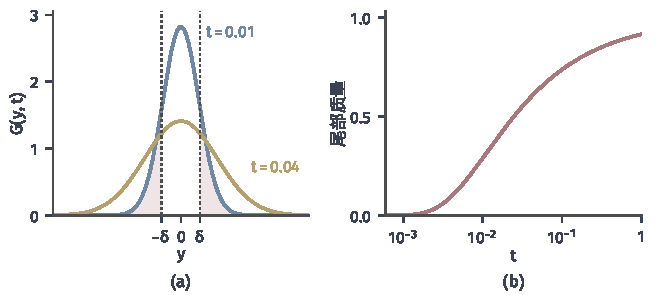
\includegraphics[width=112mm]{figures/06-differential-equations/02-partial-differential-equations/matplotlib/heat-approx-identity/figure.pdf}
  \caption{热核质量的集中。(a)$t=0.01$（蓝）与$t=0.04$（黄）的核，红色浅底是$t=0.01$时$\lvert y\rvert\geq\delta$的尾部，$\delta=0.15$。(b)该尾部质量$\operatorname{erfc}(\delta/(2\sqrt{t}))$随$t$的变化，横轴为对数。}
  \label{fig:heat-approx-identity}
\end{BookInlineFigure}

\paragraph{一致恢复}
记$C_0(\mathbb{R}^{d})$为在无穷远趋于零的连续函数，它们都有界且一致连续，所以只需讨论有界一致连续的函数。一致连续性是这里的关键：同一个$\delta$要对所有的点起作用。

\begin{theorem}[一致范数下的恢复]
\label{thm:heat-uniform-recovery}
设$u_0$在$\mathbb{R}^{d}$上有界且一致连续，特别地可以是$u_0\in C_0(\mathbb{R}^{d})$。则式~\eqref{eq:heat-convolution}给出的$u$满足
\begin{equation}
 \lim_{t\to0^+}\sup_{\bm{x}\in\mathbb{R}^{d}}\lvert u(\bm{x},t)-u_0(\bm{x})\rvert=0 .
 \label{eq:heat-uniform-recovery}
\end{equation}
\end{theorem}

\begin{proof}
因为$G$的积分为$1$，可以把$u_0(\bm{x})$写进积分。再代换$\bm{y}\mapsto\bm{x}-\bm{y}$，
\[
 u(\bm{x},t)-u_0(\bm{x})=\int G(\bm{y},t)\bigl(u_0(\bm{x}-\bm{y})-u_0(\bm{x})\bigr)\,\mathrm{d}\bm{y} .
\]
任取$\varepsilon>0$，由一致连续性取$\delta>0$，使$\lvert\bm{y}\rvert<\delta$时对所有$\bm{x}$都有$\lvert u_0(\bm{x}-\bm{y})-u_0(\bm{x})\rvert<\varepsilon$。

把积分分成$\lvert\bm{y}\rvert<\delta$和$\lvert\bm{y}\rvert\geq\delta$两部分。第一部分不超过$\varepsilon\int G=\varepsilon$。第二部分中被积的差不超过$2\lVert u_0\rVert_\infty$，于是
\[
 \lvert u(\bm{x},t)-u_0(\bm{x})\rvert\leq\varepsilon+2\lVert u_0\rVert_\infty\int_{\lvert\bm{y}\rvert\geq\delta}G(\bm{y},t)\,\mathrm{d}\bm{y} .
\]
右端与$\bm{x}$无关。由式~\eqref{eq:heat-tail}，$t$充分小时第二项小于$\varepsilon$。
\end{proof}

\paragraph{$L^p$恢复}
积分型的范数不需要逐点的连续性，$L^p$函数在平移下的连续性起到一致连续性的作用。

\begin{theorem}[$L^p$范数下的恢复]
\label{thm:heat-lp-recovery}
设$1\leq p<\infty$，$u_0\in L^p(\mathbb{R}^{d})$。则对$t>0$，$u(\cdot,t)\in L^p$，并且
\begin{equation}
 \lVert u(\cdot,t)\rVert_p\leq\lVert u_0\rVert_p,\qquad \lim_{t\to0^+}\lVert u(\cdot,t)-u_0\rVert_p=0 .
 \label{eq:heat-lp-recovery}
\end{equation}
第一个不等式对$p=\infty$也成立。
\end{theorem}

\begin{proof}
记$(\tau_{\bm{y}}u_0)(\bm{x})=u_0(\bm{x}-\bm{y})$。解是平移函数的加权平均：
\[
 u(\cdot,t)=\int G(\bm{y},t)\,\tau_{\bm{y}}u_0\,\mathrm{d}\bm{y} .
\]
积分形式的Minkowski不等式说，平均的范数不超过范数的平均，所以
\[
 \lVert u(\cdot,t)\rVert_p\leq\int G(\bm{y},t)\lVert\tau_{\bm{y}}u_0\rVert_p\,\mathrm{d}\bm{y}=\lVert u_0\rVert_p .
\]
$p=\infty$时这由$\lvert u\rvert\leq\lVert u_0\rVert_\infty\int G$直接得到。

同样地，把$u_0$写进积分后，
\[
 \lVert u(\cdot,t)-u_0\rVert_p\leq\int G(\bm{y},t)\,\lVert\tau_{\bm{y}}u_0-u_0\rVert_p\,\mathrm{d}\bm{y} .
\]
任取$\varepsilon>0$。平移在$L^p$中连续，这要求$p<\infty$，可参考\BookChapterRef{chap:function-approximation}{卷四第20章“函数逼近”}，所以存在$\delta>0$，使$\lvert\bm{y}\rvert<\delta$时$\lVert\tau_{\bm{y}}u_0-u_0\rVert_p<\varepsilon$。

分成$\lvert\bm{y}\rvert<\delta$和$\lvert\bm{y}\rvert\geq\delta$两部分。第一部分不超过$\varepsilon$。第二部分中差的范数不超过$2\lVert u_0\rVert_p$，由式~\eqref{eq:heat-tail}，$t$充分小时小于$\varepsilon$。
\end{proof}

用方框验证收敛的快慢。每条边附近$u-u_0$的绝对值在距边$s$处约为$\tfrac12\operatorname{erfc}(s/(2\sqrt{t}))$，$t$小时两条边互不干扰。边的两侧合起来积分，用$\int_0^\infty\operatorname{erfc}=1/\sqrt\pi$，每条边贡献
\[
 2\int_0^\infty\frac12\operatorname{erfc}\frac{s}{2\sqrt{t}}\,\mathrm{d}s=2\sqrt{\frac{t}{\pi}} ,
\]
所以$\lVert u(\cdot,t)-u_0\rVert_1\approx4\sqrt{t/\pi}$。$t=0.01$时这个数是$0.2257$，数值积分的结果与它一致。

图~\ref{fig:heat-recovery-norms}把几种范数放在一起。方框的$L^1$距离按$t^{1/2}$下降，$L^2$距离按$t^{1/4}$下降，一致距离却始终是$1/2$，因为边界上的解总是取$1/2$，而边的一侧初值是$1$。连续的三角形$\max\{1-\lvert x\rvert,0\}$在一致范数下收敛，折角处的下降是$2\sqrt{t/\pi}$。

\begin{BookInlineFigure}
  \centering
  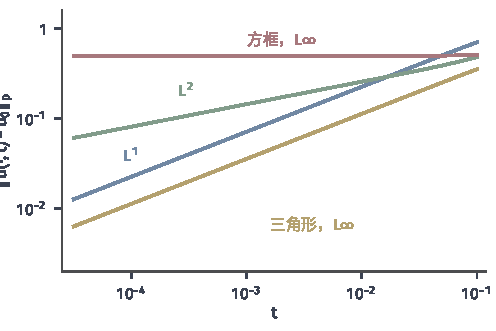
\includegraphics[width=84mm]{figures/06-differential-equations/02-partial-differential-equations/matplotlib/heat-recovery-norms/figure.pdf}
  \caption{解到初值的距离随$t$的变化，双对数坐标。方框初值$\mathbb{I}_{[-1/2,1/2]}$的$L^1$（蓝）、$L^2$（绿）、$L^\infty$（红）距离；连续三角形$\max\{1-\lvert x\rvert,0\}$的$L^\infty$距离（黄）。}
  \label{fig:heat-recovery-norms}
\end{BookInlineFigure}

\paragraph{连续点的恢复}
一般的初值只要在一点连续，解就在这一点取回初值，这是局部的结论，不需要整体的有界性。

\begin{theorem}[连续点的恢复]
\label{thm:heat-pointwise-recovery}
设$u_0$可测且满足式~\eqref{eq:heat-integrability}，在$\bm{x}_0$处连续。则
\begin{equation}
 \lim_{(\bm{x},t)\to(\bm{x}_0,0^+)}u(\bm{x},t)=u_0(\bm{x}_0) .
 \label{eq:heat-pointwise-recovery}
\end{equation}
\end{theorem}

\begin{proof}
仍利用$G$的积分为$1$，写成
\[
 u(\bm{x},t)-u_0(\bm{x}_0)=\int G(\bm{x}-\bm{y},t)\bigl(u_0(\bm{y})-u_0(\bm{x}_0)\bigr)\,\mathrm{d}\bm{y} .
\]
任取$\varepsilon>0$，取$\delta>0$使$\lvert\bm{y}-\bm{x}_0\rvert<\delta$时$\lvert u_0(\bm{y})-u_0(\bm{x}_0)\rvert<\varepsilon$。只考虑$\lvert\bm{x}-\bm{x}_0\rvert<\delta/2$。近处$\lvert\bm{y}-\bm{x}_0\rvert<\delta$的积分不超过$\varepsilon$。

在远处$\lvert\bm{y}-\bm{x}_0\rvert\geq\delta$，有$\lvert\bm{x}-\bm{y}\rvert\geq\delta/2$，并且$\lvert\bm{x}-\bm{y}\rvert$不小于$\lvert\bm{y}-\bm{x}_0\rvert/2$。

把指数平分成两半，一半用第一个下界，另一半用第二个下界：
\[
 \mathrm{e}^{-\lvert\bm{x}-\bm{y}\rvert^2/(4t)}\leq\mathrm{e}^{-\delta^2/(32t)}\,\mathrm{e}^{-\lvert\bm{y}-\bm{x}_0\rvert^2/(32t)} .
\]
限制$t\leq T/16$，并利用
\[
 \lvert\bm{y}-\bm{x}_0\rvert^2\geq\frac12\lvert\bm{y}\rvert^2-\lvert\bm{x}_0\rvert^2 ,
\]
第二个因子满足
\[
 \mathrm{e}^{-\lvert\bm{y}-\bm{x}_0\rvert^2/(32t)}\leq\mathrm{e}^{\lvert\bm{x}_0\rvert^2/(2T)}\,\mathrm{e}^{-\lvert\bm{y}\rvert^2/(4T)} .
\]

于是含$u_0(\bm{y})$的远处积分不超过
\[
 (4\pi t)^{-d/2}\,\mathrm{e}^{-\delta^2/(32t)}\,\mathrm{e}^{\lvert\bm{x}_0\rvert^2/(2T)}\int\lvert u_0(\bm{y})\rvert\,\mathrm{e}^{-\lvert\bm{y}\rvert^2/(4T)}\,\mathrm{d}\bm{y} .
\]
指数因子比$t^{-d/2}$衰减得快，所以这一项在$t\to0^+$时趋于零。

含常数$u_0(\bm{x}_0)$的远处积分不超过
\[
 \lvert u_0(\bm{x}_0)\rvert\int_{\lvert\bm{z}\rvert\geq\delta/2}G(\bm{z},t)\,\mathrm{d}\bm{z} ,
\]
由式~\eqref{eq:heat-tail}也趋于零。
\end{proof}

\paragraph{$L^\infty$的缺口}
能不能把三个定理合起来，说任意有界初值都一致恢复？不能。逐点恢复对每一点各用各的$\delta$，一致恢复要求同一个$\delta$对所有点有效，有界性也不能代替它。

取$d=1$、$u_0=\operatorname{sign}(x)$，解是$u=\operatorname{erf}(x/(2\sqrt{t}))$。对每个$x\neq0$它趋于$u_0(x)$，定理~\ref{thm:heat-pointwise-recovery}成立。但$u(0,t)=0$，$u$连续，在$0$右侧任意近处$u_0=1$而$u$接近$0$，所以对每个$t>0$，
\[
 \lVert u(\cdot,t)-u_0\rVert_\infty=1 .
\]

连续也不够。取$u_0=\sin(x^2)$，它有界连续但不一致连续。例~\ref{ex:heat-gaussian-growth}的Gauss积分对$a=\mathrm{i}$同样成立，其虚部就是解：
\[
 u(x,t)=\operatorname{Im}\Bigl[(1-4\mathrm{i}t)^{-1/2}\exp\Bigl(\frac{\mathrm{i}x^2}{1-4\mathrm{i}t}\Bigr)\Bigr] .
\]
取模得到包络$(1+16t^2)^{-1/4}\exp(-4x^2t/(1+16t^2))$，它在$\lvert x\rvert\to\infty$时趋于零。而$\sin(x^2)$在任意远处都取到$1$，所以对每个$t>0$，一致距离至少是$1$。图~\ref{fig:heat-sup-failure}画出了这两个例子。局部频率越高的地方被抹平得越快，每个$t>0$都有一片“已经抹平”的远场，它和初值相差一个固定的量。

\begin{BookInlineFigure}
  \centering
  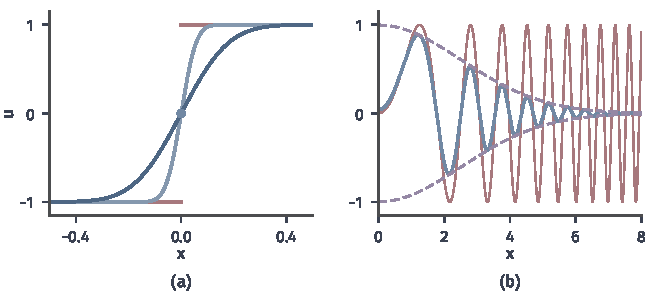
\includegraphics[width=112mm]{figures/06-differential-equations/02-partial-differential-equations/matplotlib/heat-sup-failure/figure.pdf}
  \caption{有界初值的一致恢复可能失败。(a)$u_0=\operatorname{sign}(x)$（红）与$t=0.001,0.01$的解（蓝色由浅到深），解在原点恒为零（蓝点）。(b)$u_0=\sin(x^2)$（红，细线）、$t=0.02$的解（蓝）与其包络（紫色虚线）。}
  \label{fig:heat-sup-failure}
\end{BookInlineFigure}

表~\ref{tab:heat-recovery}汇总了本节的结论。

\begin{BookInlineTable}
  \centering
  \caption{全空间热传播的初值恢复。}
  \label{tab:heat-recovery}
  \begin{tabular}{lll}
    \toprule
    初值 & 恢复方式 & 依据\\
    \midrule
    有界一致连续（含$C_0$） & 一致收敛 & 定理~\ref{thm:heat-uniform-recovery}\\
    $L^p$，$1\leq p<\infty$ & $L^p$收敛 & 定理~\ref{thm:heat-lp-recovery}\\
    满足式~\eqref{eq:heat-integrability} & 连续点处逐点收敛 & 定理~\ref{thm:heat-pointwise-recovery}\\
    一般$L^\infty$ & 一致收敛可能失败 & $\operatorname{sign}(x)$，$\sin(x^2)$\\
    \bottomrule
  \end{tabular}
\end{BookInlineTable}


\section{受迫响应}
\label{sec:heat-forced}

前面的解都由初值产生。如果棒上有持续的热源，或者端点的温度随时间改变，解又是什么？方程是线性的，答案的思路只有一条：把外部输入切成小片，每一片都当成一次自由演化的起点，再叠加起来。

\paragraph{从常微分方程到扩散}
线性常微分方程$\dot{\bm{x}}=\bm{A}\bm{x}+\bm{g}(t)$的解是
\[
 \bm{x}(t)=\mathrm{e}^{t\bm{A}}\bm{x}_0+\int_0^t\mathrm{e}^{(t-s)\bm{A}}\bm{g}(s)\,\mathrm{d}s .
\]
积分号下的读法是：时刻$s$注入的增量$\bm{g}(s)\,\mathrm{d}s$随后按齐次方程走了$t-s$的时间。

扩散的情形完全一样。时间片$[s,s+\Delta s]$内注入的热量分布大约是$f(\cdot,s)\Delta s$，它接下来自由扩散$t-s$的时间。把所有时间片的贡献加起来，令$\Delta s\to0$，得到\term{Duhamel公式}（Duhamel formula）。

\paragraph{全空间的表示}
对全空间，自由扩散由热核给出，于是
\begin{equation}
 u(\bm{x},t)=\int_{\mathbb{R}^{d}}G(\bm{x}-\bm{y},t)\,u_0(\bm{y})\,\mathrm{d}\bm{y}+\int_0^t\!\!\int_{\mathbb{R}^{d}}G(\bm{x}-\bm{y},t-s)\,f(\bm{y},s)\,\mathrm{d}\bm{y}\,\mathrm{d}s .
 \label{eq:heat-duhamel-space}
\end{equation}
图~\ref{fig:heat-duhamel-pulses}取$\lvert x\rvert<1/4$上的单位热源，持续到$t=0.5$，切成五片。较晚注入的片（深色）还很集中，较早注入的已经散开，它们的和（绿点）贴近精确的积分（蓝）。

\begin{BookInlineFigure}
  \centering
  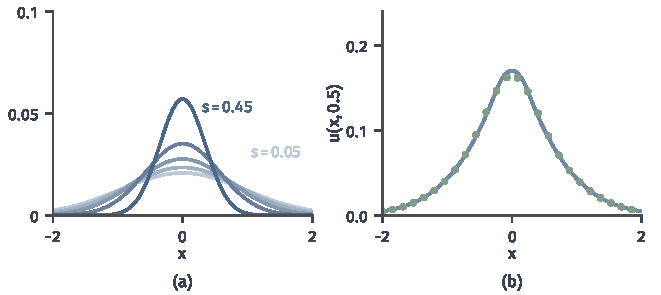
\includegraphics[width=112mm]{figures/06-differential-equations/02-partial-differential-equations/matplotlib/heat-duhamel-pulses/figure.pdf}
  \caption{热源$f=\mathbb{I}_{[-1/4,1/4]}(x)$，$0<s<0.5$，初值为零，观察时刻$t=0.5$。(a)五个时间片（$s=0.05,0.15,\ldots,0.45$，$\Delta s=0.1$）各自的响应，颜色越深注入越晚。(b)五片之和（绿点）与时间积分的精确结果（蓝）。}
  \label{fig:heat-duhamel-pulses}
\end{BookInlineFigure}

把这个想法变成定理，难点在$s\to t$时核变成奇异的。只要把时间积分靠近奇异点的一段切开，用热核收回初值的性质来处理。

\begin{theorem}[全空间的Duhamel公式]
\label{thm:heat-duhamel-space}
设$f$及其导数$\partial_tf$、$\partial_{x_i}f$、$\partial_{x_i}\partial_{x_j}f$在$\mathbb{R}^{d}\times[0,T]$上有界连续，并取$u_0=0$。则式~\eqref{eq:heat-duhamel-space}的第二项给出的$u$在$\mathbb{R}^{d}\times(0,T]$上有连续的$\partial_tu$与二阶空间偏导，并满足
\begin{equation}
 \partial_tu=\Delta u+f,\qquad \lim_{t\to0^+}\sup_{\bm{x}}\lvert u(\bm{x},t)\rvert=0 .
 \label{eq:heat-duhamel-solves}
\end{equation}
\end{theorem}

\begin{proof}
由$\int G=1$，$\lvert u(\bm{x},t)\rvert\leq t\sup\lvert f\rvert$，这给出初值条件。

为了求导，先把$\bm{y}$和$s$都换成相对量，令$\bm{y}\mapsto\bm{x}-\bm{y}$、$s\mapsto t-s$：
\[
 u(\bm{x},t)=\int_0^t\!\!\int G(\bm{y},s)\,f(\bm{x}-\bm{y},t-s)\,\mathrm{d}\bm{y}\,\mathrm{d}s .
\]
现在$\bm{x}$和$t$只出现在光滑的$f$中，可以在积分号下求导：
\[
 \Delta u=\int_0^t\!\!\int G(\bm{y},s)\,\Delta f(\bm{x}-\bm{y},t-s)\,\mathrm{d}\bm{y}\,\mathrm{d}s,
\]
\[
 \partial_tu=\int_0^t\!\!\int G(\bm{y},s)\,\partial_tf(\bm{x}-\bm{y},t-s)\,\mathrm{d}\bm{y}\,\mathrm{d}s+\int G(\bm{y},t)f(\bm{x}-\bm{y},0)\,\mathrm{d}\bm{y} .
\]
记$F(\bm{y},s)=f(\bm{x}-\bm{y},t-s)$，则$\partial_tf=-\partial_sF$，$\Delta f=\Delta_{\bm{y}}F$。相减，并把时间积分在小的$\varepsilon>0$处切开：
\[
 (\partial_t-\Delta)u=\int_\varepsilon^t\!\!\int G\,(-\partial_s-\Delta_{\bm{y}})F\,\mathrm{d}\bm{y}\,\mathrm{d}s+R_\varepsilon+\int G(\bm{y},t)F(\bm{y},t)\,\mathrm{d}\bm{y},
\]
其中$R_\varepsilon$是$[0,\varepsilon]$上的积分，由导数有界，$\lvert R_\varepsilon\rvert\leq C\varepsilon$。

第一项在$[\varepsilon,t]$上对$s$和$\bm{y}$分部积分，这里$G$光滑且快速衰减，边界只出现在$s=\varepsilon$和$s=t$：
\[
 \int_\varepsilon^t\!\!\int(\partial_sG-\Delta G)F\,\mathrm{d}\bm{y}\,\mathrm{d}s+\int G(\bm{y},\varepsilon)F(\bm{y},\varepsilon)\,\mathrm{d}\bm{y}-\int G(\bm{y},t)F(\bm{y},t)\,\mathrm{d}\bm{y} .
\]
第一个积分为零，最后一项恰好与前面的$\int G(\bm{y},t)F(\bm{y},t)\,\mathrm{d}\bm{y}$抵消。于是
\[
 (\partial_t-\Delta)u=\int G(\bm{y},\varepsilon)f(\bm{x}-\bm{y},t-\varepsilon)\,\mathrm{d}\bm{y}+R_\varepsilon .
\]
令$\varepsilon\to0^+$。$f$有界且导数有界，所以一致连续，用定理~\ref{thm:heat-uniform-recovery}同样的分段估计，右端趋于$f(\bm{x},t)$。导数的连续性由积分号下的表达式得到。
\end{proof}

这里要求$f$光滑，是因为导数都放在了$f$上。降低$f$的正则性时，经典解可能不存在，式~\eqref{eq:heat-duhamel-space}仍然可以作为一个积分定义的解，这一点在解半群一节再说。

\begin{example}[恒定点源]
\label{ex:heat-line-point-source}
实轴原点处有单位强度的恒定点源，初值为零。它不满足定理的光滑要求，但式~\eqref{eq:heat-duhamel-space}中的积分仍有意义，给出$u(x,t)=\int_0^tG(x,s)\,\mathrm{d}s$。在原点，
\[
 u(0,t)=\int_0^t\frac{\mathrm{d}s}{\sqrt{4\pi s}}=\sqrt{\frac{t}{\pi}} .
\]
$t=1$时为$0.5642$，$t=4$时为$1.1284$，无限增长。实轴上一维的点源没有稳态，因为热量散开的速度跟不上注入的速度。
\end{example}

图~\ref{fig:heat-line-point-source}对比了这一点。区间上情形不同。在$(0,1)$的中点放同样的单位点源，两端保持为零，温度有界，稳态是折线$\tfrac12\min\{x,1-x\}$，中点的值是$1/4$：吸热的端点把注入的热量带走了。

\begin{BookInlineFigure}
  \centering
  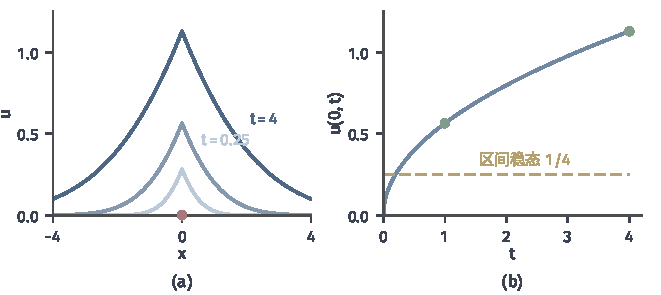
\includegraphics[width=112mm]{figures/06-differential-equations/02-partial-differential-equations/matplotlib/heat-line-point-source/figure.pdf}
  \caption{实轴上原点处的恒定单位点源（红点）。(a)$t=0.25,1,4$时的温度（蓝色由浅到深），原点处有一个折角。(b)原点温度$\sqrt{t/\pi}$（蓝）无限增长，绿点是$t=1,4$的值；黄色虚线是$(0,1)$上中点受单位点源、两端为零时的稳态值$1/4$。}
  \label{fig:heat-line-point-source}
\end{BookInlineFigure}

\paragraph{边界模式的表示}
在区间上自由演化由模式给出，同样的切片思想逐个模式进行。设$u$按$e_k$展开，系数记为$a_k(t)$，$f_k(t)=\langle f(\cdot,t),e_k\rangle$。用$e_k$检验$\partial_tu=\partial_x^2u+f$，分部积分两次，端点项因零边值而消失，每个模式得到一个独立的标量方程：
\[
 a_k'(t)=-\lambda_ka_k(t)+f_k(t) .
\]
这是一个标准的一阶线性方程，解出
\begin{equation}
 a_k(t)=\mathrm{e}^{-\lambda_kt}a_k(0)+\int_0^t\mathrm{e}^{-\lambda_k(t-s)}f_k(s)\,\mathrm{d}s .
 \label{eq:heat-duhamel-modes}
\end{equation}

把系数合起来，并定义区间上的核
\begin{equation}
 G_D(x,y,t)=\sum_{k\geq1}e_k(x)e_k(y)\mathrm{e}^{-\lambda_kt},
 \label{eq:heat-dirichlet-kernel}
\end{equation}
式~\eqref{eq:heat-duhamel-modes}就写成了与式~\eqref{eq:heat-duhamel-space}同样的形状，只是$G(x-y,t-s)$换成了$G_D(x,y,t-s)$。这个核依赖$x$和$y$两个变量，不只是它们的差，因为端点破坏了平移不变性。

当$f:[0,T]\to L^2(0,1)$连续时，由$\lvert\int_0^t\mathrm{e}^{-\lambda_k(t-s)}f_k\,\mathrm{d}s\rvert$的Cauchy--Schwarz估计，级数在$L^2$中收敛，定义了一个$L^2$值的解。若$f$、$\partial_xf$、$\partial_x^2f$在$[0,1]\times[0,T]$上连续且$f$在端点为零，分部积分两次给出$\sup_s\lvert f_k(s)\rvert\leq C/k^2$。又由时间积分的直接估计，
\[
 \lambda_k\Bigl\lvert\int_0^t\mathrm{e}^{-\lambda_k(t-s)}f_k(s)\,\mathrm{d}s\Bigr\rvert\leq\sup_s\lvert f_k(s)\rvert .
\]
于是$\sum_k\lambda_k\lvert a_k\rvert$的受迫部分可和，级数可以逐项求导，得到经典解。

\begin{example}[恒定热源趋于稳态]
\label{ex:heat-source-steady}
在$(0,1)$上取$f=1$，$u_0=0$，两端为零。系数为
\[
 f_k=\sqrt2\int_0^1\sin(k\pi x)\,\mathrm{d}x=\frac{\sqrt2\,(1-(-1)^k)}{k\pi},
\]
奇数$k$上等于$2\sqrt2/(k\pi)$，偶数$k$上为零。由式~\eqref{eq:heat-duhamel-modes}，对恒定的$f_k$积分，
\[
 a_k(t)=\frac{f_k}{\lambda_k}\bigl(1-\mathrm{e}^{-\lambda_kt}\bigr) .
\]
$t\to\infty$时$a_k\to f_k/\lambda_k$，这正是$-u''=1$、零边值的稳态解$x(1-x)/2$的系数，$-\partial_x^2$在模式坐标中就是乘以$\lambda_k$。在中点，稳态值是$1/8$。
\end{example}

这个$f$在端点不为零，上面逐项求导的充分条件不适用，但解可以直接写成稳态减去自由衰减：
\[
 u=\frac{x(1-x)}{2}-\sum_k\frac{f_k}{\lambda_k}\mathrm{e}^{-\lambda_kt}e_k .
\]
第一项是多项式，第二项属于定理~\ref{thm:heat-series}的情形，所以$t>0$时仍是经典解。

中点的值由这个级数算出，$t=0.05,0.1,0.2,0.5$时依次是
\[
 0.0463,\quad 0.0769,\quad 0.1071,\quad 0.1241 .
\]
图~\ref{fig:heat-source-steady}(b)说明每个模式按自己的速度靠近稳态，最慢的是$k=1$，高频模式几乎立刻到位。

\begin{BookInlineFigure}
  \centering
  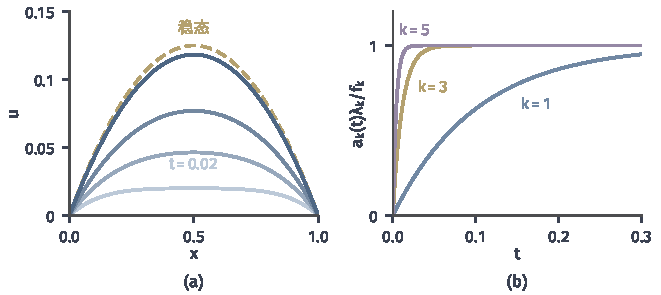
\includegraphics[width=112mm]{figures/06-differential-equations/02-partial-differential-equations/matplotlib/heat-source-steady/figure.pdf}
  \caption{恒定热源$f=1$，零边值，零初值。(a)$t=0.02,0.05,0.1,0.3$的解（蓝色由浅到深）趋于稳态$x(1-x)/2$（黄色虚线）。(b)各模式到稳态的比例$a_k(t)\lambda_k/f_k=1-\mathrm{e}^{-\lambda_kt}$，$k=1,3,5$。}
  \label{fig:heat-source-steady}
\end{BookInlineFigure}

\paragraph{非齐次边界的提升}
模式展开依赖零边值：分部积分时端点项才会消失。端点温度$u(0,t)=g_0(t)$、$u(1,t)=g_1(t)$非零时，先减去一个满足边界条件的函数，这称为\term{边界提升}（boundary lifting）。

设$g_0,g_1\in C^1[0,T]$，取线性插值
\[
 w(x,t)=(1-x)g_0(t)+xg_1(t) .
\]
令$v=u-w$。于是$v$在两端为零，而$\partial_x^2w=0$，代入原方程得到
\begin{equation}
 \partial_tv=\partial_x^2v+f-\partial_tw,\qquad v(x,0)=u_0(x)-w(x,0) .
 \label{eq:heat-lift-problem}
\end{equation}
边值变化的代价是多了一项源$-\partial_tw$，这就是要求$g_0,g_1$可微的原因。$v$现在可以用式~\eqref{eq:heat-duhamel-modes}求解。

Neumann情形要求端点斜率分别为$g_0$、$g_1$，提升不能用线性函数，因为一条直线只有一个斜率。取二次函数
\[
 w=g_0x+\frac{g_1-g_0}{2}x^2 ,
\]
这时$\partial_x^2w=g_1-g_0$不为零，$v=u-w$的源项是$f+\partial_x^2w-\partial_tw$。多维区域上可以用第~\ref{chap:elliptic-equations}章的调和函数作提升：取$\Delta w=0$、边界上$w=g$，再按上面的方式处理。

\begin{example}[一端突然加热]
\label{ex:heat-boundary-lift}
取$u_0=0$，$u(0,t)=0$，$u(1,t)=1$。提升函数是$w=x$，不随时间变化，于是$v$满足无源的热方程，初值$-x$。$x$在$e_k$上的坐标是$\sqrt2(-1)^{k+1}/(k\pi)$，所以
\[
 u(x,t)=x+\sum_{k\geq1}\frac{2(-1)^k}{k\pi}\,\mathrm{e}^{-k^2\pi^2t}\sin(k\pi x) .
\]
在中点，$t=0.05,0.1,0.2,0.5$的温度分别是
\[
 0.1138,\quad 0.2628,\quad 0.4116,\quad 0.4954 ,
\]
趋于稳态$w(1/2)=1/2$。
\end{example}

这个例子的初值和边值在$(1,0)$处矛盾，$v$的初值$-x$在$x=1$不为零，所以属于定理~\ref{thm:heat-series}的$L^2$情形，$t>0$时光滑。图~\ref{fig:heat-boundary-lift}中，(a)是$v$的衰减，(b)是加回$w$之后的$u$。

\begin{BookInlineFigure}
  \centering
  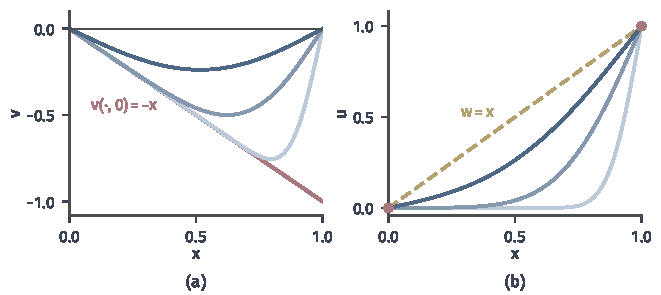
\includegraphics[width=112mm]{figures/06-differential-equations/02-partial-differential-equations/matplotlib/heat-boundary-lift/figure.pdf}
  \caption{边界提升，$u(0,t)=0$，$u(1,t)=1$，$u_0=0$，$t=0.005,0.03,0.1$（蓝色由浅到深）。(a)$v=u-w$，初值$-x$（红），两端为零。(b)$u=w+v$，黄色虚线是提升函数$w=x$，红点是边值。}
  \label{fig:heat-boundary-lift}
\end{BookInlineFigure}

\paragraph{全空间公式不能照搬}
既然有了卷积公式，能否直接把区间上的初值代进去？把三角形延拓成零，用实轴的核做卷积，图~\ref{fig:heat-wholeline-vs-interval}(a)的黄线就是结果。在$t=0.05$时它在端点的值约$0.111$，并不等于边值$0$，棒外的“真空”也被当成了可以吸收热量的材料。

对有特殊几何的区间，可以用\term{像源法}（method of images）修正。把初值奇延拓，再按周期$2$延拓，图~\ref{fig:heat-wholeline-vs-interval}(b)的红线就是这个延拓。这个函数在$x=0,1$两侧反对称，实轴上的卷积保持对称性，所以解在这些点始终为零。

\begin{BookInlineFigure}
  \centering
  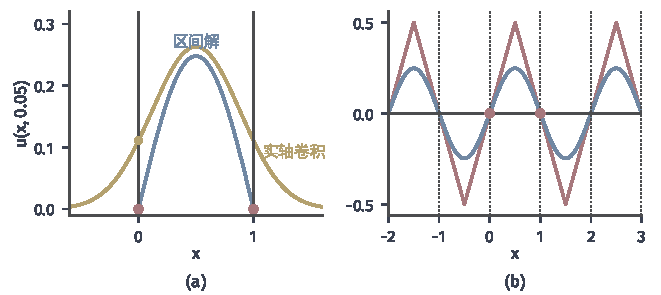
\includegraphics[width=112mm]{figures/06-differential-equations/02-partial-differential-equations/matplotlib/heat-wholeline-vs-interval/figure.pdf}
  \caption{实轴卷积与区间问题，三角形初值，$t=0.05$。(a)区间解（蓝）在端点（红点）为零；把三角形延拓为零后的实轴卷积（黄）在端点的值约$0.111$。深灰竖线是棒的端点。(b)奇延拓并按周期$2$延拓的初值（红）与实轴卷积（蓝），解在每个整数点为零。}
  \label{fig:heat-wholeline-vs-interval}
\end{BookInlineFigure}

用公式写出来，把周期延拓代入卷积，就得到另一种形式的区间核：
\begin{equation}
 G_D(x,y,t)=\sum_{n\in\mathbb{Z}}\bigl(G(x-y+2n,t)-G(x+y+2n,t)\bigr) .
 \label{eq:heat-image-kernel}
\end{equation}
它和式~\eqref{eq:heat-dirichlet-kernel}是同一个函数的两种写法，因为两者给出同一个问题的解，而解是唯一的，唯一性在第~\ref{sec:heat-properties}节证明。像源的写法在$t$小时收敛极快，只需$n=0$的项；模式的写法在$t$大时收敛极快，只需前几项。对图中的例子数值计算$u(1/2,0.05)$，两种写法都得到$0.24796$。一般区域没有这种反射结构，边界的作用需要由模式或其他方法处理。


\section{解的性质}
\label{sec:heat-properties}

上面几节的解都有公式，公式只存在于少数几何形状上。一般区域、一般数据时能断定什么？下面研究四个量：总热量、最高最低温度、平方积分、光滑程度。每个量的变化规律都来自对方程本身的一次计算，不需要解的表达式，并且在估计中明确写出需要什么边界和源项条件。

\subsection{质量变化}
\label{sec:heat-mass}

棒里的总热量会怎样变？这是守恒律的积分形式，它的结论最直接。记$M(t)=\int_\Omega u(\bm{x},t)\,\mathrm{d}\bm{x}$。

\begin{theorem}[质量平衡]
\label{thm:heat-mass-balance}
设$\Omega$是有界开集，边界分段$C^1$，$u$在$\overline\Omega\times(0,T]$上有连续的$\partial_tu$和二阶空间偏导，满足$\partial_tu=\Delta u+f$，$f$连续。则对$0<t\leq T$，
\begin{equation}
 M'(t)=\int_\Omega f\,\mathrm{d}\bm{x}+\int_{\partial\Omega}\partial_{\bm{n}}u\,\mathrm{d}S .
 \label{eq:heat-mass-balance}
\end{equation}
\end{theorem}

\begin{proof}
被积函数连续，可以在积分号下对$t$求导：$M'(t)=\int_\Omega(\Delta u+f)\,\mathrm{d}\bm{x}$。由散度定理，$\Delta u=\nabla\cdot\nabla u$的体积分等于$\partial_{\bm{n}}u$的边界积分。这就是式~\eqref{eq:heat-mass-balance}。
\end{proof}

右端两项是两个不同的来源：内部源项的贡献和穿过边界的净通量。于是可以分情形读。

无源且零Neumann条件时，右端为零，总质量守恒。无源且零Dirichlet条件时，边界项一般不为零。设$u\geq0$，边界上$u=0$是最小值，温度沿外法向下降，$\partial_{\bm{n}}u\leq0$，所以$M'\leq0$，这种吸收边界让质量流失。

全空间没有边界，但需要无穷远处的衰减代替它。最直接的条件是$u_0\in L^1(\mathbb{R}^{d})$，这时由Fubini定理和$\int G=1$，
\[
 \int_{\mathbb{R}^{d}}u(\bm{x},t)\,\mathrm{d}\bm{x}=\int_{\mathbb{R}^{d}}u_0(\bm{y})\int_{\mathbb{R}^{d}}G(\bm{x}-\bm{y},t)\,\mathrm{d}\bm{x}\,\mathrm{d}\bm{y}=\int_{\mathbb{R}^{d}}u_0(\bm{y})\,\mathrm{d}\bm{y} .
\]
这里不需要任何关于导数在无穷远的假设。如果想用式~\eqref{eq:heat-mass-balance}在大球上取极限，就要证明大球面上的通量趋于零，这正是“适当衰减”的含义。

回到三角形。由式~\eqref{eq:heat-sine-solution}逐项积分，Dirichlet情形的质量是
\[
 M(t)=\sum_{k\text{ 奇}}\frac{8\sin(k\pi/2)}{k^3\pi^3}\,\mathrm{e}^{-k^2\pi^2t} .
\]
$t=0$时求和得$1/4$，$t=0.02,0.05,0.1,0.2$时依次约为
\[
 0.2102,\quad 0.1574,\quad 0.0962,\quad 0.0358 .
\]
Neumann情形$M$恒为$1/4$。对称性使两端的流出相同，式~\eqref{eq:heat-mass-balance}给出$M'=-2\partial_xu(0,t)$，$t=0.1$时左端斜率约为$0.4745$，流出率约为$0.949$，图~\ref{fig:heat-mass-balance}(b)用$M$的差商核对了这个等式。

有源时两项相互竞争。图~\ref{fig:heat-mass-balance}(c)取$f=1$，$u_0=0$。Dirichlet情形下，随着温度升高，边界流出变大，最终内部注入速率$1$被两端流出抵消，每端的斜率大小是$1/2$，质量趋于稳态的积分$\int_0^1x(1-x)/2\,\mathrm{d}x=1/12$。Neumann情形没有出口，$M(t)=t$无限增长，没有稳态，这对应着椭圆Neumann问题的相容条件$\int f=0$不成立。

\begin{BookInlineFigure}
  \centering
  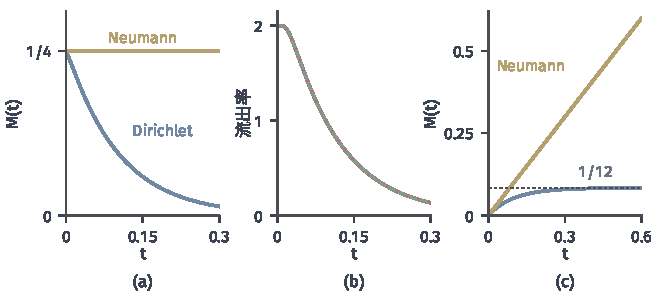
\includegraphics[width=112mm]{figures/06-differential-equations/02-partial-differential-equations/matplotlib/heat-mass-balance/figure.pdf}
  \caption{总热量的变化。(a)三角形初值、无源：Dirichlet（蓝）流失，Neumann（黄）不变。(b)Dirichlet情形的边界流出率$2\partial_xu(0,t)$（红）与$-M'(t)$的差商（绿色虚线），两者重合。(c)$f=1$、$u_0=0$：Dirichlet（蓝）趋于$1/12$，Neumann（黄）线性增长。}
  \label{fig:heat-mass-balance}
\end{BookInlineFigure}

\subsection{最大值原理}
\label{sec:heat-maximum}

没有热源时，棒内能不能出现比开始时和端点都热的点？物理上不能，热量只往低处流。数学上的结论需要指明温度的最大值可能出现在哪些地方，这就要看时空区域的边界中哪一部分真正影响解。

\paragraph{抛物边界}
记$\Omega_T=\Omega\times(0,T]$。称底面与侧面的并
\[
 \Gamma_T=(\overline\Omega\times\{0\})\cup(\partial\Omega\times[0,T])
\]
为\term{抛物边界}（parabolic boundary），它就是给定数据的那部分，图~\ref{fig:heat-parabolic-boundary}。顶面$t=T$不在其中，因为信息只从过去流向未来，那里的值由方程决定。

\begin{BookInlineFigure}
  \centering
  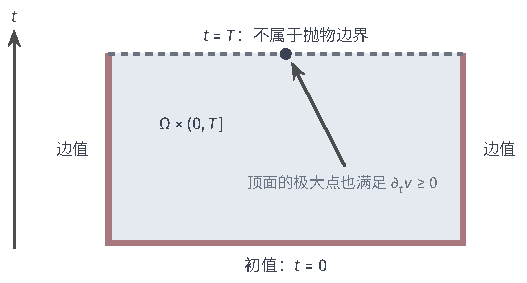
\includegraphics[width=90mm]{figures/06-differential-equations/02-partial-differential-equations/tikz/heat-parabolic-boundary/figure.pdf}
  \caption{时空矩形$\Omega\times(0,T]$的抛物边界（红色粗线）由底面和两条侧边组成，顶面（虚线）不属于它。顶面上若有极大点（黑点），那里的时间导数只能从过去一侧计算，符号仍然与方程矛盾，这正是定理的证明要点。}
  \label{fig:heat-parabolic-boundary}
\end{BookInlineFigure}

\begin{theorem}[弱最大值原理]
\label{thm:heat-weak-max}
设$\Omega$是有界开集，$u\in C(\overline\Omega\times[0,T])$，在$\Omega_T$上$\partial_tu$和二阶空间偏导连续，且$\partial_tu-\Delta u\leq0$。则
\begin{equation}
 \max_{\overline\Omega\times[0,T]}u=\max_{\Gamma_T}u .
 \label{eq:heat-weak-max}
\end{equation}
\end{theorem}

\begin{proof}
如果严格不等式$\partial_tv-\Delta v<0$成立，论证很短，所以先制造严格性。任取$\varepsilon>0$，令$v=u-\varepsilon t$，则
\[
 \partial_tv-\Delta v=\partial_tu-\Delta u-\varepsilon<0 .
\]
$v$在紧集上连续，在某点$(\bm{x}_0,t_0)$取得最大值。假设这一点不在$\Gamma_T$上，即$\bm{x}_0\in\Omega$，$0<t_0\leq T$。

固定$t_0$，$\bm{x}_0$是$v(\cdot,t_0)$的内部极大点，Hessian半负定，于是$\Delta v(\bm{x}_0,t_0)\leq0$。固定$\bm{x}_0$看时间：若$t_0<T$，一阶条件给出$\partial_tv=0$；若$t_0=T$，$v(\bm{x}_0,t)\leq v(\bm{x}_0,T)$对$t<T$成立，左导数给出$\partial_tv\geq0$。无论哪种情形，
\[
 \partial_tv-\Delta v\geq0,
\]
与严格不等式矛盾。所以$v$的最大值在$\Gamma_T$上取到。由$0\leq\varepsilon t\leq\varepsilon T$，
\[
 \max u\leq\max v+\varepsilon T=\max_{\Gamma_T}v+\varepsilon T\leq\max_{\Gamma_T}u+\varepsilon T .
\]
令$\varepsilon\to0$，得$\max u\leq\max_{\Gamma_T}u$。反方向的不等式成立是因为$\Gamma_T$是整个闭集的子集。
\end{proof}

条件$\partial_tu-\Delta u\leq0$的含义是内部不产生热量，可以吸热。对$-u$用定理，就得到$\partial_tu-\Delta u\geq0$时最小值在$\Gamma_T$上取到。图~\ref{fig:heat-max-envelope}中初值是$\sin(\pi x)+\sin(5\pi x)$，负的小凹陷很快被填平，最大值单调下降，最小值从$-0.198$上升到$0$，都不越出初值和边界值的范围。

\begin{BookInlineFigure}
  \centering
  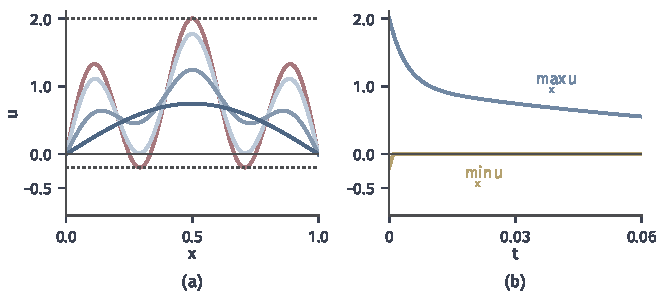
\includegraphics[width=112mm]{figures/06-differential-equations/02-partial-differential-equations/matplotlib/heat-max-envelope/figure.pdf}
  \caption{最大值原理的例子，$u_0=\sin(\pi x)+\sin(5\pi x)$（红），两端为零。(a)$t=0.001,0.005,0.03$的解（蓝色由浅到深），两条点线是初值的最大值$2$和最小值$-0.198$。(b)$\max_xu$（蓝）单调下降，$\min_xu$（黄）单调上升到$0$。}
  \label{fig:heat-max-envelope}
\end{BookInlineFigure}

这里要注意定理比较的是抛物边界上的值。零Neumann条件下侧面的值未知，定理不能直接说最大值在底面。一维时可以用偶延拓把隔热端点变成对称的内部点，再用全空间的结论，就知道隔热棒的最高温也不超过初值的最高温。一般区域上的同一结论需要边界点处法向导数的符号引理，篇幅较长，读者可查阅抛物方程的教材。

\paragraph{比较、唯一与连续依赖}
线性方程的两个解相减仍是解，把弱最大值原理用在差上，立刻得到几条结论。

\begin{theorem}[比较原理与唯一性]
\label{thm:heat-comparison}
设$\Omega$是有界开集，$u_1,u_2$满足定理~\ref{thm:heat-weak-max}的正则性，记$Lu=\partial_tu-\Delta u$。
\begin{enumerate}
 \item 若在$\Omega_T$上$Lu_1\leq Lu_2$，在$\Gamma_T$上$u_1\leq u_2$，则处处$u_1\leq u_2$。
 \item 若$Lu_i=f_i$，记$F=\sup_{\Omega_T}\lvert f_1-f_2\rvert$，则
 \begin{equation}
  \max\lvert u_1-u_2\rvert\leq\max_{\Gamma_T}\lvert u_1-u_2\rvert+TF .
  \label{eq:heat-max-stability}
 \end{equation}
 \item 特别地，Dirichlet初边值问题的经典解至多一个。
\end{enumerate}
\end{theorem}

\begin{proof}
(1)对$u_1-u_2$用定理~\ref{thm:heat-weak-max}。

(2)令$w=u_1-u_2-Ft$，则$\partial_tw-\Delta w=f_1-f_2-F\leq0$。由定理~\ref{thm:heat-weak-max}和$-Ft\leq0$，
\[
 \max(u_1-u_2)\leq\max w+FT\leq\max_{\Gamma_T}(u_1-u_2)+FT .
\]
交换$u_1$与$u_2$得到另一方向。

(3)在式~\eqref{eq:heat-max-stability}中令数据相同，右端为零。
\end{proof}

比较原理使我们能用简单的函数夹住解。例如例~\ref{ex:heat-source-steady}中$f=1$、$u_0=0$：与$w=t$比较，$\partial_tw-\partial_x^2w=1=f$，抛物边界上$u\leq w$，于是$u\leq t$；再与稳态$x(1-x)/2$比较，又有$u\leq x(1-x)/2$。前面算出$t=0.05$时中点值是$0.0463$，确实不超过$0.05$，也不超过$0.125$。

\paragraph{全空间与增长限制}
有界区域的证明用到了最大值存在，这在全空间不再自动成立，结论本身也可能失败。存在一族Tikhonov解，由
\[
 u(x,t)=\sum_{m\geq0}\frac{x^{2m}}{(2m)!}\,\phi^{(m)}(t),\qquad \phi(t)=\mathrm{e}^{-t^{-\alpha}}\ (\alpha>1,\ t>0),\quad \phi(0)=0
\]
给出，它在实轴上满足热方程，初值为零，却不恒为零。这个例子的收敛性验证较长，读者可查阅偏微分方程的教材。它的增长比$\mathrm{e}^{ax^2}$还快，这是无穷远处传进来的“幽灵热量”。下面的定理说明，只要禁止这样的增长，最大值原理就恢复了。

\begin{theorem}[全空间的最大值原理]
\label{thm:heat-whole-max}
设$u\in C(\mathbb{R}^{d}\times[0,T])$，在$\mathbb{R}^{d}\times(0,T]$上$\partial_tu$和二阶空间偏导连续，$\partial_tu-\Delta u\leq0$，并存在常数$A,a>0$，使
\begin{equation}
 u(\bm{x},t)\leq A\,\mathrm{e}^{a\lvert\bm{x}\rvert^2},\qquad \bm{x}\in\mathbb{R}^{d},\ 0\leq t\leq T .
 \label{eq:heat-growth}
\end{equation}
若$M_0=\sup u_0<\infty$，则$u\leq M_0$处处成立。特别地，若两个解的绝对值都满足式~\eqref{eq:heat-growth}这样的界，初值相同则解相同。
\end{theorem}

\begin{proof}
先设$4aT<1$，取$\varepsilon>0$使$4a(T+\varepsilon)<1$，并记$a+\gamma=1/(4(T+\varepsilon))$，$\gamma>0$。固定$\bm{y}\in\mathbb{R}^{d}$、$\mu>0$，引入一个向无穷增长、满足方程的比较函数。记$\rho=T+\varepsilon-t>0$，令
\[
 w(\bm{x},t)=\rho^{-d/2}\exp\Bigl(\frac{\lvert\bm{x}-\bm{y}\rvert^2}{4\rho}\Bigr) .
\]
直接求导，$\partial_tw$和$\Delta w$都等于$\bigl(\tfrac{d}{2\rho}+\tfrac{\lvert\bm{x}-\bm{y}\rvert^2}{4\rho^2}\bigr)w$，所以$\partial_tw=\Delta w$。令$v=u-\mu w$，则$\partial_tv-\Delta v\leq0$。

在球$B_r(\bm{y})$上用定理~\ref{thm:heat-weak-max}，只需看抛物边界。底面上$w>0$，所以$v\leq u_0\leq M_0$。侧面$\lvert\bm{x}-\bm{y}\rvert=r$上，用式~\eqref{eq:heat-growth}和$\rho\leq T+\varepsilon$，
\[
 v\leq A\,\mathrm{e}^{a(\lvert\bm{y}\rvert+r)^2}-\mu\,(T+\varepsilon)^{-d/2}\,\mathrm{e}^{(a+\gamma)r^2} .
\]
$r\to\infty$时第二项的指数系数$a+\gamma$大于第一项的$a$，右端趋于$-\infty$，于是$r$足够大时$v\leq M_0$。

由定理~\ref{thm:heat-weak-max}，$v\leq M_0$在球内成立。在球心取值，得$u(\bm{y},t)\leq M_0+\mu\,w(\bm{y},t)$。$w(\bm{y},t)=\rho^{-d/2}$有界，令$\mu\to0$，得$u(\bm{y},t)\leq M_0$。

一般的$T$，把$[0,T]$分成长度不超过$1/(8a)$的小段，逐段应用上面的结论，每一段的初值都不超过$M_0$。唯一性：两个解的差及其相反数都满足定理的条件，初值的上确界为零，差恒为零。
\end{proof}

增长条件的常数$a$可以任意大，$T$也可以任意大，不过$\mathrm{e}^{a\lvert\bm{x}\rvert^2}$这样的阶不能放宽，Tikhonov解正好越过这条线。这与定理~\ref{thm:heat-convolution-smooth}的积分条件相呼应：两者都以Gauss函数的增长为界。

\subsection{能量估计}
\label{sec:heat-energy}

最大值原理控制的是最坏的一点，并且依赖边界上的符号。另一种度量是平方积分，它在两种齐次边界下都表现得很好，而且自然地连接到弱解。记$E(t)=\tfrac12\lVert u(\cdot,t)\rVert_2^2$。

\begin{theorem}[能量估计]
\label{thm:heat-energy}
设$\Omega$是有界开集，边界分段$C^1$，$u\in C(\overline\Omega\times[0,T])$，在$\overline\Omega\times(0,T]$上$\partial_tu$和二阶空间偏导连续，满足$\partial_tu=\Delta u+f$（$f$连续）及零Dirichlet条件或零Neumann条件。则对$0<t\leq T$，
\begin{equation}
 \frac12\frac{\mathrm{d}}{\mathrm{d}t}\lVert u\rVert_2^2+\lVert\nabla u\rVert_2^2=\langle f,u\rangle .
 \label{eq:heat-energy-identity}
\end{equation}
无源时，对$0<t\leq T$还有
\begin{equation}
 \frac12\lVert u(\cdot,t)\rVert_2^2+\int_0^t\lVert\nabla u\rVert_2^2\,\mathrm{d}s=\frac12\lVert u_0\rVert_2^2 .
 \label{eq:heat-energy-integrated}
\end{equation}
一般地，零Neumann时取$\mu=0$，零Dirichlet时取$\mu=1/C_P^2$，其中$C_P$是Poincaré常数，则
\begin{equation}
 \lVert u(\cdot,t)\rVert_2\leq\mathrm{e}^{-\mu t}\lVert u_0\rVert_2+\int_0^t\mathrm{e}^{-\mu(t-s)}\lVert f(\cdot,s)\rVert_2\,\mathrm{d}s .
 \label{eq:heat-energy-bound}
\end{equation}
\end{theorem}

\begin{proof}
用$u$乘方程并在$\Omega$上积分。由Green公式，
\[
 \int_\Omega u\,\Delta u\,\mathrm{d}\bm{x}=-\lVert\nabla u\rVert_2^2+\int_{\partial\Omega}u\,\partial_{\bm{n}}u\,\mathrm{d}S .
\]
两种边界条件都使边界积分为零，一种因为$u=0$，另一种因为$\partial_{\bm{n}}u=0$。这就是式~\eqref{eq:heat-energy-identity}。

无源时把式~\eqref{eq:heat-energy-identity}在$[\varepsilon,t]$上积分。令$\varepsilon\to0^+$，$u$在闭集上连续，$E(\varepsilon)\to E(0)$；由单调收敛定理，梯度项收敛，这样得到式~\eqref{eq:heat-energy-integrated}。

为了得到式~\eqref{eq:heat-energy-bound}，想对$\lVert u\rVert_2$求导，但它在零点不可微，所以任取$\varepsilon>0$，令$y=(\lVert u\rVert_2^2+\varepsilon)^{1/2}$。由式~\eqref{eq:heat-energy-identity}和Cauchy--Schwarz不等式，以及$\lVert\nabla u\rVert_2^2\geq\mu\lVert u\rVert_2^2$（Neumann时$\mu=0$，这个不等式平凡；Dirichlet时是Poincaré不等式），
\[
 y\,y'\leq-\mu\lVert u\rVert_2^2+\lVert f\rVert_2\lVert u\rVert_2 .
\]
两边除以$y>0$，用$\lVert u\rVert_2\leq y$和$\lVert u\rVert_2^2/y\geq y-\sqrt\varepsilon$，
\[
 y'\leq-\mu y+\mu\sqrt\varepsilon+\lVert f\rVert_2 .
\]
乘积分因子$\mathrm{e}^{\mu t}$积分，令$\varepsilon\to0$，就得到式~\eqref{eq:heat-energy-bound}。
\end{proof}

式~\eqref{eq:heat-energy-integrated}有两层含义。第一，能量单调下降，下降的量正是梯度的平方积分，起伏越大，耗散越快。第二，即使初值只属于$L^2$，梯度在时间上的平方积分也不超过$\tfrac12\lVert u_0\rVert_2^2$，这是后面平滑效应的积分形式。

在$(0,1)$上零Dirichlet时最优的$C_P=1/\pi$，式~\eqref{eq:heat-energy-bound}无源时就是式~\eqref{eq:heat-series-decay}，能量方法不用模式得到了同样的衰减率。

\paragraph{用于比较两组数据}
方程线性，两个解的差满足同类问题，把式~\eqref{eq:heat-energy-bound}用在差上就是对数据的连续依赖：
\begin{equation}
 \lVert u_1(t)-u_2(t)\rVert_2\leq\mathrm{e}^{-\mu t}\lVert u_{1,0}-u_{2,0}\rVert_2+\int_0^t\mathrm{e}^{-\mu(t-s)}\lVert f_1-f_2\rVert_2\,\mathrm{d}s .
 \label{eq:heat-energy-stability}
\end{equation}
数据相同则差为零，所以这也给出唯一性，并且包括零Neumann问题，这是弱最大值原理没有直接给出的。

\begin{example}[两组初值的差]
\label{ex:heat-energy-difference}
在$(0,1)$上取零边值，$u_{1,0}$为三角形，第二组初值是
\[
 u_{2,0}=u_{1,0}+\tfrac{1}{10}(\sin\pi x+\sin3\pi x) .
\]
差的初值范数是$\tfrac{1}{10}\sqrt{1/2+1/2}=0.1$，而差本身是
\[
 u_2-u_1=\tfrac{1}{10}\bigl(\mathrm{e}^{-\pi^2t}\sin\pi x+\mathrm{e}^{-9\pi^2t}\sin3\pi x\bigr) .
\]
由正交性，其范数是$\tfrac{1}{10}(\tfrac12\mathrm{e}^{-2\pi^2t}+\tfrac12\mathrm{e}^{-18\pi^2t})^{1/2}$，不超过上界$0.1\,\mathrm{e}^{-\pi^2t}$。
\end{example}

\paragraph{能量衰减与质量守恒}
能量和质量是两个不同的量，隔热棒把这一点显示得最清楚：总质量不变，能量仍在减少。由Cauchy--Schwarz不等式，$M^2\leq\lvert\Omega\rvert\,\lVert u\rVert_2^2$，等号当且仅当$u$为常数。所以在质量固定时，均匀分布的能量最小，扩散正是把温度推向这个最小能量的状态。

三角形的初始能量是$\tfrac12\int_0^1u_0^2\,\mathrm{d}x=1/24$。在隔热棒中，最终温度是$1/4$，最终能量是$\tfrac12(1/4)^2=1/32$。两者相差的$1/96$由式~\eqref{eq:heat-energy-integrated}全部以梯度平方的时间积分耗散掉。接冰水时，能量和质量都趋于零，图~\ref{fig:heat-energy-mass}(a)。

\begin{BookInlineFigure}
  \centering
  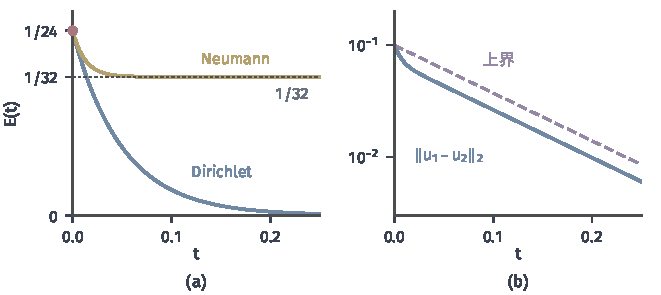
\includegraphics[width=112mm]{figures/06-differential-equations/02-partial-differential-equations/matplotlib/heat-energy-mass/figure.pdf}
  \caption{能量。(a)三角形初值（初始能量$1/24$，红点）的$E(t)$：Neumann（黄）下降到$1/32$后停止，Dirichlet（蓝）趋于$0$。(b)例~\ref{ex:heat-energy-difference}的差的$L^2$范数（蓝）与上界$0.1\,\mathrm{e}^{-\pi^2t}$（紫色虚线），纵轴为对数。}
  \label{fig:heat-energy-mass}
\end{BookInlineFigure}

上面的定理对经典解陈述。解也可以只在弱形式下成立：它在时间上平方可积地取值于$H^1_0(\Omega)$，对几乎每个$t$和每个$v\in H^1_0(\Omega)$有
\[
 \frac{\mathrm{d}}{\mathrm{d}t}\langle u,v\rangle+a(u,v)=\langle f,v\rangle ,
\]
其中$a(u,v)=\int_\Omega\nabla u\cdot\nabla v$，同样的能量等式仍然成立，取$v=u$的合法性需要取值于函数空间的时间导数理论，证明较长，读者可查阅抛物方程的教材。

表~\ref{tab:heat-three-measures}把三个度量放在一起。

\begin{BookInlineTable}
  \centering
  \caption{无源热方程的三种度量。}
  \label{tab:heat-three-measures}
  \begin{tabular}{llll}
    \toprule
    量 & 零Dirichlet & 零Neumann & 控制方式\\
    \midrule
    总质量 & 流失 & 守恒 & 边界通量\\
    最大值 & 不超过数据 & 不超过初值 & 符号结构\\
    能量 & 趋于$0$ & 趋于均匀态能量 & 梯度耗散\\
    \bottomrule
  \end{tabular}
\end{BookInlineTable}

\subsection{正时间平滑}
\label{sec:heat-smoothing}

定理~\ref{thm:heat-series}和定理~\ref{thm:heat-convolution-smooth}都说，$t>0$时解立即变成无穷光滑。这种\term{平滑效应}（smoothing effect）有多强？导数能大到什么程度？

\paragraph{全空间：把导数放到核上}
卷积的导数可以放在核上：$\partial^\alpha_{\bm{x}}u=(\partial^\alpha G)*u_0$。初值无需可导，所有的导数都由光滑的核承担，代价只是核的导数的大小。

\begin{theorem}[全空间的平滑估计]
\label{thm:heat-smoothing}
设$1\leq p\leq\infty$，$u_0\in L^p(\mathbb{R}^{d})$，$\alpha$是多重指标。则存在只依赖$\alpha$和$d$的常数$C_\alpha$，使对$t>0$，
\begin{equation}
 \lVert\partial^\alpha_{\bm{x}}u(\cdot,t)\rVert_p\leq C_\alpha\,t^{-\lvert\alpha\rvert/2}\,\lVert u_0\rVert_p .
 \label{eq:heat-smoothing}
\end{equation}
\end{theorem}

\begin{proof}
$L^p$函数满足式~\eqref{eq:heat-integrability}：由Hölder不等式，Gauss函数属于$L^{p'}$。于是定理~\ref{thm:heat-convolution-smooth}允许在积分号下求导。用定理~\ref{thm:heat-lp-recovery}证明中的Minkowski不等式，
\[
 \lVert\partial^\alpha u(\cdot,t)\rVert_p\leq\lVert\partial^\alpha G(\cdot,t)\rVert_1\,\lVert u_0\rVert_p .
\]
由尺度关系~\eqref{eq:heat-kernel-scaling}求导，
\[
 \partial^\alpha G(\bm{x},t)=t^{-(d+\lvert\alpha\rvert)/2}(\partial^\alpha G)(\bm{x}/\sqrt{t},1) .
\]
积分时代换$\bm{x}=\sqrt{t}\,\bm{z}$，因子$t^{d/2}$抵消，于是
\[
 \lVert\partial^\alpha G(\cdot,t)\rVert_1=t^{-\lvert\alpha\rvert/2}\lVert\partial^\alpha G(\cdot,1)\rVert_1 .
\]
把最后这个有限的$L^1$范数取作$C_\alpha$。
\end{proof}

一维$\alpha=1$时常数可以算出来。$G(\cdot,t)$是单峰函数，它的导数的$L^1$范数等于全变差，是峰值的两倍：
\[
 \lVert\partial_xG(\cdot,t)\rVert_1=2G(0,t)=\frac{1}{\sqrt{\pi t}} .
\]
于是
\[
 \lVert\partial_xu(\cdot,t)\rVert_\infty\leq\frac{\lVert u_0\rVert_\infty}{\sqrt{\pi t}} .
\]
这个常数不能再小：$u_0=\operatorname{sign}(x)$时$u=\operatorname{erf}(x/(2\sqrt{t}))$，在原点的斜率恰好是$1/\sqrt{\pi t}$，等号成立。

同样的办法还能把可积性换成有界性。卷积不超过核的上确界乘以$\lVert u_0\rVert_1$，于是
\[
 \lVert u(\cdot,t)\rVert_\infty\leq(4\pi t)^{-d/2}\lVert u_0\rVert_1 .
\]
这说明一点上的尖峰无法存留，只要总量有限，高度就被核的峰值控制。

\paragraph{区间：谱系数的压制}
有界区间上同样的结论由系数得到。对式~\eqref{eq:heat-sine-solution}，$\partial_x^mu$的系数比$u$多一个因子$(k\pi)^m$，而$\sqrt2\sin k\pi x$、$\sqrt2\cos k\pi x$都是标准正交系，所以
\[
 \lVert\partial_x^mu(\cdot,t)\rVert_2^2=\sum_k\lambda_k^m\,\mathrm{e}^{-2\lambda_kt}c_k^2\leq\Bigl(\sup_{\lambda>0}\lambda^m\mathrm{e}^{-2\lambda t}\Bigr)\sum_kc_k^2 .
\]
函数$\lambda^m\mathrm{e}^{-2\lambda t}$在$\lambda=m/(2t)$处取最大值，代入得到
\begin{equation}
 \lVert\partial_x^mu(\cdot,t)\rVert_2\leq\Bigl(\frac{m}{2\mathrm{e}\,t}\Bigr)^{m/2}\lVert u_0\rVert_2,\qquad t>0 .
 \label{eq:heat-spectral-smoothing}
\end{equation}
这和式~\eqref{eq:heat-smoothing}的$t^{-m/2}$一致。指数因子不管多小的$t$，都压得住任何多项式因子，这就是无穷光滑的来源；只是$t$越小，压制所需的频率越高，界就越大。

\paragraph{估计变差与初值的光滑性}
式~\eqref{eq:heat-smoothing}在$t\to0^+$时趋于无穷，这不说明解在变坏，而是说明界要为最粗糙的初值留有余地。初值的导数已经有界时，估计不必如此。

导数和卷积可交换：若$u_0$有界且一阶导数有界，则$\partial_xu=G*\partial_xu_0$，于是
\[
 \lVert\partial_xu(\cdot,t)\rVert_\infty\leq\lVert\partial_xu_0\rVert_\infty ,
\]
$t\to0^+$时没有奇性。解保持初值原有的光滑程度，只对超出这个程度的导数付出$t^{-1/2}$的代价。

图~\ref{fig:heat-smoothing-rates}用两个初值把这两件事分开。跳跃$\operatorname{sign}(x)$的一阶导数的界是$1/\sqrt{\pi t}$。折线$-\lvert x\rvert$的解满足$\partial_xu=-\operatorname{erf}(x/(2\sqrt{t}))$，一阶导数的界恒为$1$，二阶导数$\partial_x^2u=-2G(x,t)$的界是$1/\sqrt{\pi t}$：多出来的一阶导数才要付代价。跳跃的二阶导数代价是$t^{-1}$，正好多一个$t^{-1/2}$。

\begin{BookInlineFigure}
  \centering
  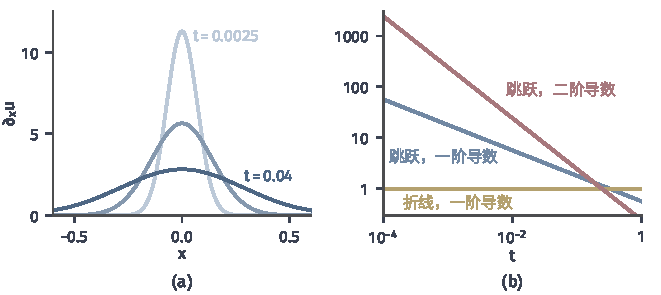
\includegraphics[width=112mm]{figures/06-differential-equations/02-partial-differential-equations/matplotlib/heat-smoothing-rates/figure.pdf}
  \caption{平滑的代价。(a)跳跃$\operatorname{sign}(x)$的解的斜率$2G(x,t)$，$t=0.0025,0.01,0.04$（蓝色由浅到深）。(b)精确的上确界，双对数坐标：跳跃的$\lVert\partial_xu\rVert_\infty=1/\sqrt{\pi t}$（蓝），跳跃的$\lVert\partial_x^2u\rVert_\infty\propto t^{-1}$（红），折线$-\lvert x\rvert$的$\lVert\partial_xu\rVert_\infty=1$（黄）。}
  \label{fig:heat-smoothing-rates}
\end{BookInlineFigure}


\section{解半群}
\label{sec:heat-semigroup}

无源时，时刻$t$的解由初值完全决定，这是一个映射。在矩阵情形，它就是$\mathrm{e}^{t\bm{A}}$，走两段时间等于把两个指数相乘。热方程的解映射是否也构成这样的结构？它的“$\bm{A}$”是什么？这需要先确定函数空间。

\paragraph{解算子与时间拼接}
把初值$u_0$映到时刻$t$的解，记为$S(t)u_0$。全空间上$S(t)u_0=G(\cdot,t)*u_0$，区间上$S(t)$把坐标$c_k$乘以$\mathrm{e}^{-\lambda_kt}$。在区间上，时间拼接就是指数相加：
\[
 \mathrm{e}^{-\lambda_k(t+s)}=\mathrm{e}^{-\lambda_kt}\,\mathrm{e}^{-\lambda_ks} .
\]

全空间上，$S(t+s)=S(t)S(s)$等价于热核的卷积恒等式
\begin{equation}
 G(\cdot,t)*G(\cdot,s)=G(\cdot,t+s),\qquad t,s>0 .
 \label{eq:heat-kernel-semigroup}
\end{equation}
证明最快的办法是取Fourier变换：左边的变换是$\mathrm{e}^{-4\pi^2\lvert\bm{\xi}\rvert^2t}\mathrm{e}^{-4\pi^2\lvert\bm{\xi}\rvert^2s}$，右边的变换是$\mathrm{e}^{-4\pi^2\lvert\bm{\xi}\rvert^2(t+s)}$，两者相等，而两边都是$L^1$函数，$L^1$上Fourier变换是单射。这个恒等式也可以从方差读出：两个独立的Gauss扰动相加，方差相加，$2t+2s=2(t+s)$。

有了式~\eqref{eq:heat-kernel-semigroup}，由Fubini定理得到$S(t)S(s)u_0=S(t+s)u_0$。图~\ref{fig:heat-semigroup-composition}用数值卷积核对了这一点：分两步走与一步走到同样的终点，差别是离散误差。这就是从时刻$s$的状态重新开始，后续演化不需要知道更早的历史。

\begin{BookInlineFigure}
  \centering
  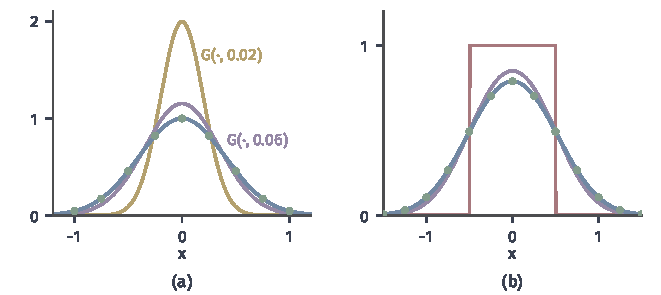
\includegraphics[width=112mm]{figures/06-differential-equations/02-partial-differential-equations/matplotlib/heat-semigroup-composition/figure.pdf}
  \caption{时间拼接。(a)$G(\cdot,0.02)$（黄）与$G(\cdot,0.06)$（紫）的数值卷积（绿点）落在$G(\cdot,0.08)$（蓝）上。(b)方框（红）先走$0.06$（紫）再走$0.02$（绿点），与一步走$0.08$的解（蓝）一致。}
  \label{fig:heat-semigroup-composition}
\end{BookInlineFigure}

\paragraph{强连续半群}
把这些性质抽象出来。注意其中只有$t\geq0$，反向一般不存在，这是“半”字的含义。

\begin{definition}[强连续半群]
\label{def:heat-c0-semigroup}
设$X$是Banach空间，$\{S(t)\}_{t\geq0}$是$X$上的有界线性算子族。若
\begin{equation}
 S(0)=I,\qquad S(t+s)=S(t)S(s),\qquad \lim_{t\to0^+}\lVert S(t)x-x\rVert_X=0
 \label{eq:heat-c0-semigroup}
\end{equation}
对所有$t,s\geq0$和$x\in X$成立，则称它是\term{强连续半群}（strongly continuous semigroup）。若还有$\lVert S(t)\rVert\leq1$，称为\term{压缩半群}（contraction semigroup）。把$u_0$映到解的这样一族算子称为\term{解半群}（solution semigroup）。
\end{definition}

强连续是一个与空间有关的性质，这正是上一节初值恢复定理的用武之地。由定理~\ref{thm:heat-uniform-recovery}和定理~\ref{thm:heat-lp-recovery}，全空间热半群在$C_0(\mathbb{R}^{d})$、有界一致连续函数空间及$L^p$（$1\leq p<\infty$）上是强连续的压缩半群；这里用到的是$S(t)$把这些空间映到自身，$C_0$的情形可由控制收敛定理得到。在$L^\infty$上$S(t)$仍是压缩的半群，却不强连续，$\operatorname{sign}(x)$就是反例。

强连续只要求对每个固定的$x$收敛，不要求算子范数收敛。对区间上的$L^2$半群，算子是对角的，所以
\[
 \lVert S(t)-I\rVert=\sup_k\bigl(1-\mathrm{e}^{-\lambda_kt}\bigr)=1,\qquad t>0 .
\]
无论$t$多小，足够高的频率都还没有“被恢复”，图~\ref{fig:heat-unbounded-generator}(a)。对矩阵则$\lVert\mathrm{e}^{t\bm{A}}-\bm{I}\rVert\to0$，这是有限维和无限维的本质差别之一。

\paragraph{生成元}
矩阵可以由指数函数在零点的导数取回：
\[
 \bm{A}=\lim_{t\to0}\frac{\mathrm{e}^{t\bm{A}}-\bm{I}}{t} .
\]
对半群做同样的事，极限只对部分$x$存在。

\begin{definition}[生成元]
\label{def:heat-generator}
设$\{S(t)\}$是$X$上的强连续半群。对$x\in X$考虑差商的极限
\begin{equation}
 Ax=\lim_{t\to0^+}\frac{S(t)x-x}{t} .
 \label{eq:heat-generator-limit}
\end{equation}
使这个极限在$X$中存在的$x$构成子空间$D(A)$。称$A$为半群的\term{生成元}（generator），$D(A)$为它的定义域。
\end{definition}

区间上的情形可以完全算出来，而且把边界条件的位置显露出来。

\begin{theorem}[区间热半群的生成元]
\label{thm:heat-generator}
在$X=L^2(0,1)$上，设$S(t)$是零Dirichlet条件的半群，$u=\sum_kc_ke_k$。则
\begin{equation}
 D(A)=\Bigl\{u:\sum_k\lambda_k^2c_k^2<\infty\Bigr\}=H^2(0,1)\cap H^1_0(0,1),\qquad Au=u'' .
 \label{eq:heat-generator-dirichlet}
\end{equation}
零Neumann条件时，用$\tilde{e}_k$的坐标写同样的条件，得到
\begin{equation}
 D(A)=\{u\in H^2(0,1):u'(0)=u'(1)=0\},\qquad Au=u'' .
 \label{eq:heat-generator-neumann}
\end{equation}
\end{theorem}

\begin{proof}
只写Dirichlet情形，Neumann情形把正弦换成余弦，并加上$k=0$一项。

设$\sum_k\lambda_k^2c_k^2<\infty$，令$y=-\sum_k\lambda_kc_ke_k$。按坐标计算
\[
 \Bigl\lVert\frac{S(t)u-u}{t}-y\Bigr\rVert_2^2=\sum_k\Bigl(\frac{\mathrm{e}^{-\lambda_kt}-1}{t}+\lambda_k\Bigr)^2c_k^2 .
\]
由$0\leq1-\mathrm{e}^{-\lambda t}\leq\lambda t$，括号中的量属于$[0,\lambda_k]$，每一项不超过可和的$\lambda_k^2c_k^2$，又对每个$k$趋于零。由控制收敛定理，和趋于零，所以$u\in D(A)$且$Au=y$。

反过来，若极限$y$存在，取第$k$个坐标，$\langle y,e_k\rangle=-\lambda_kc_k$，由Parseval等式，$\sum_k\lambda_k^2c_k^2$等于$\lVert y\rVert_2^2$，有限。

现在识别这个集合。若$\sum_k\lambda_k^2c_k^2<\infty$，部分和$u_N$在$H^2$中是Cauchy列，因为
\[
 \lVert u_N''\rVert_2^2=\sum_{k\leq N}\lambda_k^2c_k^2,\qquad \lVert u_N'\rVert_2^2=\sum_{k\leq N}\lambda_kc_k^2 .
\]
极限$u\in H^2$，$H^1$收敛蕴含端点值收敛，所以$u(0)=u(1)=0$，且$u''=-\sum_k\lambda_kc_ke_k=y$。

若$u\in H^2\cap H^1_0$，分部积分两次，端点项因$u$和$e_k$在两端为零而消失，
\[
 \langle u'',e_k\rangle=\langle u,e_k''\rangle=-\lambda_kc_k .
\]
由Parseval等式，$\sum_k\lambda_k^2c_k^2$等于$\lVert u''\rVert_2^2$，有限。
\end{proof}

这个定理说明，两种边界条件对应同一个微分表达式$u''$，却是两个不同的算子，图~\ref{fig:heat-generator-domain}。边界条件不在表达式里，而在定义域里。前面分离变量时边界条件决定可用的模式，这里是同一件事的算子语言。

\begin{BookInlineFigure}
  \centering
  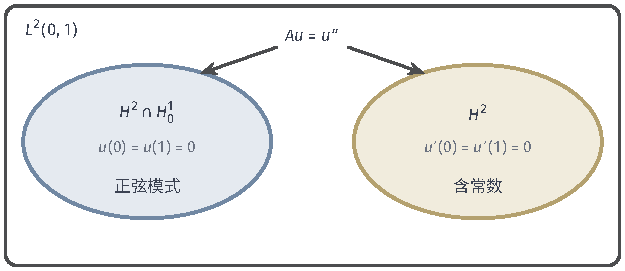
\includegraphics[width=105mm]{figures/06-differential-equations/02-partial-differential-equations/tikz/heat-generator-domain/figure.pdf}
  \caption{同一个表达式$Au=u''$的两个定义域，都是$L^2(0,1)$的稠密子空间。左（蓝）是零Dirichlet条件，由正弦模式张成；右（黄）是零Neumann条件，包含常数，生成不同的半群。}
  \label{fig:heat-generator-domain}
\end{BookInlineFigure}

生成元是无界算子：$\lVert Ae_k\rVert_2=k^2\pi^2\to\infty$，这也是$\lVert S(t)-I\rVert$不趋于零的原因。于是$\mathrm{e}^{tA}$不能用幂级数定义，一般的$u\in L^2$根本不在$D(A^n)$中。空间离散后，这种无界性表现为矩阵最大特征值随网格加细而增长，约为$4/h^2$，图~\ref{fig:heat-unbounded-generator}(b)。

\begin{BookInlineFigure}
  \centering
  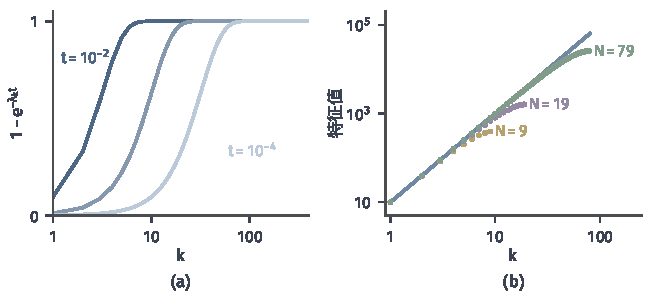
\includegraphics[width=112mm]{figures/06-differential-equations/02-partial-differential-equations/matplotlib/heat-unbounded-generator/figure.pdf}
  \caption{生成元的无界性。(a)$1-\mathrm{e}^{-\lambda_kt}$对$k$的关系，$t=10^{-2},10^{-3},10^{-4}$（蓝色由深到浅），对每个$t$都随$k$增大趋于$1$。(b)离散Laplace矩阵的特征值$4h^{-2}\sin^2(k\pi h/2)$，$N=9,19,79$（点），蓝线是$\lambda_k=k^2\pi^2$，网格越细能到达的特征值越大。}
  \label{fig:heat-unbounded-generator}
\end{BookInlineFigure}

\paragraph{一般区域与源项}
一般的有界区域上，可以用第~\ref{chap:elliptic-equations}章的双线性型定义生成元。令
\[
 a(u,v)=\int_\Omega\nabla u\cdot\nabla v\,\mathrm{d}\bm{x} .
\]
$D(A)$由这样的$u\in H^1_0(\Omega)$组成：存在$g\in L^2(\Omega)$，使$a(u,v)=-\langle g,v\rangle$对所有$v\in H^1_0(\Omega)$成立，此时$Au=g$。Dirichlet边界藏在空间$H^1_0$里，$g$是弱意义下的$\Delta u$。

$-A$的逆是椭圆问题的解算子，它在$L^2(\Omega)$上紧且自伴。由紧自伴算子的谱定理，存在$L^2(\Omega)$的标准正交基$\{e_k\}$和$0<\lambda_1\leq\lambda_2\leq\cdots\to\infty$，于是半群可以直接写成
\begin{equation}
 S(t)u_0=\sum_k\mathrm{e}^{-\lambda_kt}\langle u_0,e_k\rangle e_k ,
 \label{eq:heat-spectral-semigroup}
\end{equation}
谱定理可参考\BookChapterRef{chap:operator-spectra}{卷四第18章“算子谱”}。一般的算子何时生成半群由Hille--Yosida定理回答，它的证明需要预解式的估计，这里的算子已经有了显式的谱表示，所以用不到它。

源项的公式回到前面的切片思想。设$f:[0,T]\to X$连续，
\begin{equation}
 u(t)=S(t)u_0+\int_0^tS(t-s)f(s)\,\mathrm{d}s
 \label{eq:heat-mild}
\end{equation}
称为\term{温和解}（mild solution）。它只要求半群存在，而不要求$u$可微。强连续性和$\lVert S(t)\rVert\leq1$保证被积函数连续，积分在$X$中存在。数据足够好时，它与经典解一致，式~\eqref{eq:heat-duhamel-space}和式~\eqref{eq:heat-duhamel-modes}是它的两个具体形式。

最后，半群和椭圆问题之间有一个简单的关系。在零Dirichlet的情形下，把式~\eqref{eq:heat-spectral-semigroup}对时间从$0$积到$\infty$，每个模式的因子积分为$1/\lambda_k$，所以对$f\in L^2(\Omega)$，
\[
 \int_0^\infty S(t)f\,\mathrm{d}t=(-A)^{-1}f .
\]
恒定热源在无穷长时间内累积的响应，就是Poisson问题的解。例~\ref{ex:heat-source-steady}中$a_k\to f_k/\lambda_k$是这个等式的坐标形式。

与矩阵的对照见表~\ref{tab:heat-matrix-analogy}。

\begin{BookInlineTable}
  \centering
  \caption{矩阵指数与热半群的对照。}
  \label{tab:heat-matrix-analogy}
  \begin{tabular}{lll}
    \toprule
    & 线性常微分方程 & 热方程\\
    \midrule
    演化算子 & $\mathrm{e}^{t\bm{A}}$，$t\in\mathbb{R}$ & $S(t)$，$t\geq0$\\
    生成元 & 有界，处处有定义 & 无界，定义域含边界条件\\
    小时间连续 & 按算子范数 & 只按每个初值\\
    输入响应 & 常数变易公式 & Duhamel公式（温和解）\\
    \bottomrule
  \end{tabular}
\end{BookInlineTable}


\section{逆热问题}
\label{sec:heat-inverse}

设想测得了棒在时刻$T$的温度，想知道时刻$0$的温度。这称为\term{逆热问题}（backward heat problem）。方程本身可逆吗？正向问题适定，反向问题是否同样？

\paragraph{高频被放大}
在$(0,1)$上取零边值，$u(\cdot,T)$的坐标是$y_k=\mathrm{e}^{-\lambda_kT}c_k$。形式上，初值的坐标由$c_k=\mathrm{e}^{\lambda_kT}y_k$恢复，这一步把每个坐标放大$\mathrm{e}^{\lambda_kT}$倍。$T=0.05$时，
\[
 \mathrm{e}^{\lambda_1T}\approx1.64,\quad \mathrm{e}^{\lambda_3T}\approx84.9,\quad \mathrm{e}^{\lambda_5T}\approx2.3\times10^{5},\quad \mathrm{e}^{\lambda_7T}\approx3.2\times10^{10} .
\]
测量总有误差。正向传播把高频压没了，反向传播要把它放大回来，噪声也跟着放大。

图~\ref{fig:heat-inverse-amplify}(b)、(c)显示了问题的另一面：两个明显不同的初值，到$T=0.05$时几乎无法区分。差的部分是$0.12\sin(11\pi x)$，放大因子使它在终态只剩约$10^{-27}$，任何测量都看不出来。

\begin{BookInlineFigure}
  \centering
  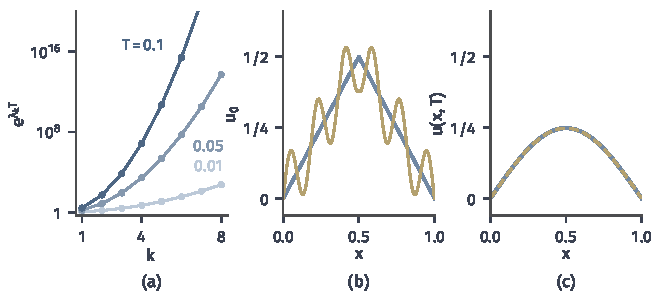
\includegraphics[width=112mm]{figures/06-differential-equations/02-partial-differential-equations/matplotlib/heat-inverse-amplify/figure.pdf}
  \caption{反向恢复的困难。(a)放大因子$\mathrm{e}^{\lambda_kT}$，$T=0.01,0.05,0.1$（蓝色由浅到深），纵轴为对数。(b)三角形初值（蓝）及加上$0.12\sin(11\pi x)$的初值（黄）。(c)二者在$T=0.05$时的解，两条曲线重合。}
  \label{fig:heat-inverse-amplify}
\end{BookInlineFigure}

\paragraph{不适定性}
正向映射是单射，所以终态确实决定初态。可是Hadamard的三条要求中，存在性和连续依赖都失败，这就是\term{不适定问题}（ill-posed problem）的情形。

\begin{theorem}[逆热问题的不适定性]
\label{thm:heat-inverse-illposed}
设$S(T):L^2(0,1)\to L^2(0,1)$是零Dirichlet条件的解算子，$T>0$。
\begin{enumerate}
 \item $S(T)$是单射；$y=\sum_ky_ke_k$属于其值域，当且仅当
 \begin{equation}
  \sum_k\mathrm{e}^{2\lambda_kT}y_k^2<\infty .
  \label{eq:heat-inverse-range}
 \end{equation}
 \item 逆映射不连续：存在$\lVert\eta_n\rVert_2\to0$的扰动，使$\lVert S(T)^{-1}\eta_n\rVert_2\to\infty$。
\end{enumerate}
\end{theorem}

\begin{proof}
(1)若$S(T)u_0=0$，则$\mathrm{e}^{-\lambda_kT}c_k=0$，所以全部$c_k=0$。$y=S(T)u_0$当且仅当$c_k=\mathrm{e}^{\lambda_kT}y_k$平方可和，这就是式~\eqref{eq:heat-inverse-range}。

(2)取$\eta_n=\mathrm{e}^{-\lambda_nT/2}e_n$。它的范数$\mathrm{e}^{-\lambda_nT/2}\to0$。而
\[
 S(T)^{-1}\eta_n=\mathrm{e}^{\lambda_nT/2}e_n,
\]
范数趋于无穷。
\end{proof}

式~\eqref{eq:heat-inverse-range}说，只有极其光滑的函数才是可能的终态。一个带噪声的观测几乎一定不满足它，形式公式的级数发散。

\paragraph{中间时刻的稳定性}
恢复$t=0$是不可能稳定的，但恢复稍早的时刻$0<t<T$好得多，只要预先知道初值有界。由Hölder不等式，取指数$T/(T-t)$与$T/t$，把$c_k^2\mathrm{e}^{-2\lambda_kt}$写成$(c_k^2)^{1-t/T}(c_k^2\mathrm{e}^{-2\lambda_kT})^{t/T}$，
\begin{equation}
 \lVert u(\cdot,t)\rVert_2\leq\lVert u_0\rVert_2^{\,1-t/T}\,\lVert u(\cdot,T)\rVert_2^{\,t/T} .
 \label{eq:heat-log-convexity}
\end{equation}
如果$\lVert u_0\rVert_2\leq R$，两个候选解的差也满足这个不等式，所以观测误差$\delta$在时刻$t$产生至多$(2R)^{1-t/T}\delta^{t/T}$的误差。这个指数$t/T$随$t\to0$退化为零，反映出$t=0$处失去稳定性。

\paragraph{用截断恢复}
放弃高频，只恢复可靠的部分。设观测$y=S(T)u_0+\eta$，$\lVert\eta\rVert_2\leq\delta$。截断重建是
\begin{equation}
 u^{N}=\sum_{k\leq N}\mathrm{e}^{\lambda_kT}\langle y,e_k\rangle\,e_k .
 \label{eq:heat-truncated}
\end{equation}

\begin{theorem}[截断重建的误差]
\label{thm:heat-truncation}
若$u_0\in H^1_0(0,1)$，$\lVert u_0'\rVert_2\leq R$，则
\begin{equation}
 \lVert u^{N}-u_0\rVert_2\leq\mathrm{e}^{\lambda_NT}\delta+\frac{R}{\sqrt{\lambda_{N+1}}} .
 \label{eq:heat-truncation-error}
\end{equation}
\end{theorem}

\begin{proof}
观测的坐标是衰减后的真值加噪声的坐标，代入式~\eqref{eq:heat-truncated}，
\[
 u^{N}-u_0=\sum_{k\leq N}\mathrm{e}^{\lambda_kT}\langle\eta,e_k\rangle e_k-\sum_{k>N}c_ke_k .
\]
第一个和的范数不超过$\mathrm{e}^{\lambda_NT}\delta$，因为每个放大因子不超过$\mathrm{e}^{\lambda_NT}$。第二个和的平方范数是$\sum_{k>N}c_k^2$，由定理~\ref{thm:heat-series}证明中的分部积分和Parseval等式，$\sum_k\lambda_kc_k^2$等于$\lVert u_0'\rVert_2^2$，不超过$R^2$，于是
\[
 \sum_{k>N}c_k^2\leq\frac{1}{\lambda_{N+1}}\sum_{k>N}\lambda_kc_k^2\leq\frac{R^2}{\lambda_{N+1}} .
\]
\end{proof}

误差分成两半：噪声放大随$N$指数增长，截断偏差随$N$缓慢下降。使两者平衡，大致要求$\mathrm{e}^{\lambda_NT}\delta\sim1$，即
\begin{equation}
 N\approx\frac{1}{\pi}\sqrt{\frac{\ln(1/\delta)}{T}} .
 \label{eq:heat-recoverable-scale}
\end{equation}
这个数决定了可恢复的最细尺度。$T=0.05$时，$\delta=10^{-3},10^{-6},10^{-12}$对应$N\approx3.7,\,5.3,\,7.5$。测量精度提高到平方，可恢复的频率只增加到$\sqrt2$倍；相应的偏差只按$1/\sqrt{\ln(1/\delta)}$下降。

\begin{example}[三角形的重建]
\label{ex:heat-inverse-tent}
取三角形初值，$T=0.05$，每个奇数模式的观测都有固定误差$\eta_k=10^{-3}$。第$k$个模式的恢复误差是$10^{-3}\mathrm{e}^{\lambda_kT}$，$k=1,3,5$时分别为$0.0016$、$0.0849$、$228$。而真实系数只有$c_1\approx0.2866$，$c_3\approx-0.0318$，$c_5\approx0.0115$：$k=3$的恢复误差已经比系数本身大，$k=5$则完全被噪声淹没。总误差如表~\ref{tab:heat-inverse-error}，最好的选择是只保留$k=1$。
\end{example}

\begin{BookInlineTable}
  \centering
  \caption{三角形初值的截断重建误差，$T=0.05$，每个奇数模式的观测误差为$10^{-3}$，取$k\leq N$的奇数模式。}
  \label{tab:heat-inverse-error}
  \begin{tabular}{llll}
    \toprule
    $N$ & 噪声放大 & 截断偏差 & $L^2$总误差\\
    \midrule
    $1$ & $0.0016$ & $0.0347$ & $0.0348$\\
    $3$ & $0.0849$ & $0.0138$ & $0.0860$\\
    $5$ & $228$ & $0.0078$ & $228$\\
    \bottomrule
  \end{tabular}
\end{BookInlineTable}

图~\ref{fig:heat-inverse-recon}画出了这三种重建。$N=1$时得到一条平滑的拱形，整体位置正确；$N=3$时噪声开始主导；$N=5$时重建的幅度达到数百，已经和三角形毫无关系。

\begin{BookInlineFigure}
  \centering
  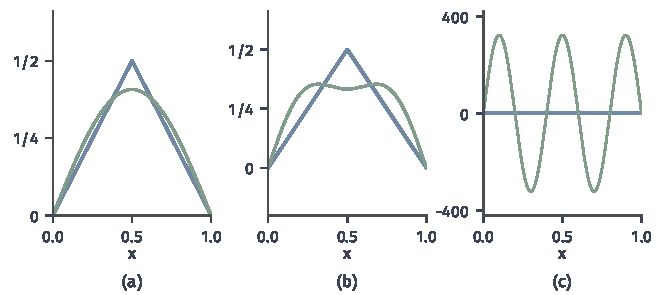
\includegraphics[width=112mm]{figures/06-differential-equations/02-partial-differential-equations/matplotlib/heat-inverse-recon/figure.pdf}
  \caption{截断重建，$T=0.05$，每个奇数模式的观测误差为$10^{-3}$。蓝线是真实的三角形，绿线是$u^{N}$。(a)$N=1$。(b)$N=3$。(c)$N=5$，注意纵轴范围。}
  \label{fig:heat-inverse-recon}
\end{BookInlineFigure}

\paragraph{Tikhonov滤波}
截断是硬开关。\term{Tikhonov正则化}（Tikhonov regularization）用平滑的滤波代替它。设$\sigma_k=\mathrm{e}^{-\lambda_kT}$，取$\alpha>0$，极小化
\[
 \lVert S(T)v-y\rVert_2^2+\alpha\lVert v\rVert_2^2 .
\]
这个问题按坐标分开，第$k$个坐标是一元二次函数，解为
\begin{equation}
 v_k=\frac{\sigma_k}{\sigma_k^2+\alpha}\,y_k .
 \label{eq:heat-tikhonov}
\end{equation}
增益$\sigma/(\sigma^2+\alpha)$在$\sigma=\sqrt\alpha$处最大，最大值是$1/(2\sqrt\alpha)$，所以噪声放大不超过这个数。$\sigma\gg\sqrt\alpha$的低频几乎按$1/\sigma$恢复，$\sigma\ll\sqrt\alpha$的高频被压到零。

取$\alpha=10^{-4}$，增益的上限是$50$。$T=0.05$时，$k=1,3,5$的增益分别是$1.64$、$49.3$、$0.044$，未正则化时是$1.64$、$84.9$、$2.3\times10^5$。图~\ref{fig:heat-inverse-tradeoff}(a)是不同噪声水平下总误差随$N$的变化，呈现先降后升的形状；图~\ref{fig:heat-inverse-tradeoff}(b)比较了三种增益。

\begin{BookInlineFigure}
  \centering
  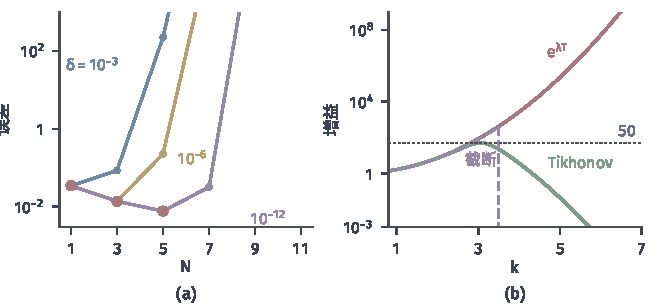
\includegraphics[width=112mm]{figures/06-differential-equations/02-partial-differential-equations/matplotlib/heat-inverse-tradeoff/figure.pdf}
  \caption{噪声与可恢复尺度。(a)三角形初值，$T=0.05$，每个奇数模式的观测误差$\delta=10^{-3},10^{-6},10^{-12}$时$L^2$总误差随$N$的变化，红点是最优的$N$。(b)作为连续变量$k$的增益：未正则化的$\mathrm{e}^{\lambda T}$（红）、截断（紫色虚线，示意取在$k=3.5$）、$\alpha=10^{-4}$的Tikhonov滤波（绿），点线是增益上限$50$。}
  \label{fig:heat-inverse-tradeoff}
\end{BookInlineFigure}

正则化并不能恢复已经丢失的信息，它只是诚实地放弃了高频，用先验（如初值的范数有界）换取稳定。正向过程越能抹平细节，反向过程就越难找回细节，这两者是同一个衰减因子的两面。


\section{本章小结}
\label{sec:heat-summary}

本章回答了一个局部规律怎样决定整体演化的问题。每一点向邻居的平均值靠拢，写成方程是$\partial_tu=\Delta u+f$，再加上一个初值和边界条件，问题就确定了。固定温度和无通量是两种不同的物理规定，前者让热量流出，后者保留一个零模式。

同一个传播过程有四种描述，它们各有适用的场合，见表~\ref{tab:heat-summary}。边界模式把问题对角化，高频衰减得快，零模式不衰减；热核把一点的影响写成Gauss钟形，宽度按$\sqrt{t}$增长；能量和极值估计不需要显式公式；半群把解看成算子，边界条件落在生成元的定义域中。

\begin{BookInlineTable}
  \centering
  \caption{同一扩散过程的四种描述。}
  \label{tab:heat-summary}
  \begin{tabular}{lll}
    \toprule
    描述 & 适用情形 & 看到的结构\\
    \midrule
    边界模式 & 有界区域，零边值 & 独立模式按$\mathrm{e}^{-\lambda_kt}$衰减\\
    热核卷积 & 全空间，受增长限制 & Gauss平均，$\sqrt{t}$尺度\\
    能量与极值 & 一般区域，明确的边界 & 耗散、比较、唯一性\\
    解半群 & 选定函数空间 & 时间拼接，无界生成元\\
    \bottomrule
  \end{tabular}
\end{BookInlineTable}

结论的成立范围都有明确的边界。初值恢复的方式取决于数据：有界一致连续初值一致恢复，$L^p$初值（$1\leq p<\infty$）在$L^p$中恢复，一般$L^\infty$初值只在连续点逐点恢复。全空间的唯一性要限制增长，否则有Tikhonov解。经典解的公式需要相应的正则性和相容性，粗糙数据时只能在$L^2$或弱的意义下理解。估计都是有限时间的，长期行为的一般理论不在本卷。

持续输入和非齐次边界都归结到同一条原则：线性叠加，把输入切片后逐片自由演化。这个原则要求已经知道自由演化；非零边值要先提升，全空间卷积不能直接用于有界区域。

平滑效应是扩散最突出的特点，也是逆问题困难的根源。正向过程在$t>0$时把高频按指数压低，反向恢复必须把它们放大回来，所以可恢复的频率只随测量精度的对数增长。

第~\ref{chap:wave-equations}章的波动方程有两个初值、有限的传播速度和守恒的能量，可以与这里的耗散和瞬间影响逐条比较。随机路径、转移概率和Fokker--Planck方程给出的概率解释不属于本卷范围，空间离散则在第~\ref{chap:pde-numerical-methods}章讨论。


\chapter{波动方程（补充）}
\label{chap:wave-equations}

拨动一根绷紧的弦然后松手。指尖离开的瞬间弦是一条折线，速度处处为零；片刻之后折角分成两个，各自向两端跑去，碰到琴桥又翻转回来。如果换成用小锤敲击，弦的初始形状是平的，却有一段初速度，随后的运动又完全不同。第~\ref{chap:diffusion-equations}章的热传导只要知道初始温度，这里却要同时知道初始位移和初始速度，时间导数多了一阶，整个演化的性格就变了。

最直接的差别有三个。温度的鼓包会被抹平，再也回不到原样，弦上的波却带着折角一直走下去，没有衰减，也没有变光滑。热方程在正时刻处处感受到初值的变化，弦上的一点却要等波跑过来才知道远处发生了什么。扩散的平方范数单调减小，弦的动能和弹性能却彼此转换，总量不变。

本章把这几点讲清楚，作为椭圆和扩散两章之外的补充。先由弦的受力写出方程，比较各种端点条件。一维实轴上的解可以完全写出来，它把初始数据分成左右两列行波，并告诉我们每个时空点依赖哪段初值。端点的作用用反射解释，区间上的解用模式展开，边界条件决定可以用哪些模式。

外力和边界驱动的影响用脉冲叠加算出。最后两节离开具体公式：能量恒等式给出守恒和唯一性，局部能量估计说明扰动不会超出传播锥，这两个结论在高维同样成立。高维的波没有左右两列的分解，本章只讨论能在高维保留下来的结论，具体的高维解公式不作推导。

\section{波动问题}
\label{sec:wave-problem}

一根弦的运动由什么决定？先从受力写出方程，看清位移、速度、波速和外力各自的位置，再讨论弦的端点能怎样约束运动。

\paragraph{从张力到方程}
设弦静止时沿$x$轴拉直，线密度（单位长度的质量）为常数$\rho>0$，张力大小为常数$\kappa>0$。记$u(x,t)$为点$x$在时刻$t$的竖直位移。我们只考虑小振动：斜率满足$\lvert\partial_xu\rvert\ll1$，弦上各点只沿竖直方向运动。

取一小段$[x,x+\Delta x]$，如图~\ref{fig:wave-string-element}。它的两端各受一个沿切线方向的张力，水平分量近似抵消，竖直分量决定这一小段的加速度。设切线与水平方向的夹角为$\theta$，则$\tan\theta=\partial_xu$，于是
\[
 \sin\theta=\frac{\partial_xu}{\sqrt{1+(\partial_xu)^{2}}}=\partial_xu+O\bigl(\lvert\partial_xu\rvert^{3}\bigr).
\]
小斜率假设在这里起作用：竖直分量可以用$\kappa\,\partial_xu$代替，弦的伸长也只是斜率的二阶量，所以张力保持常数。

\begin{BookInlineFigure}
  \centering
  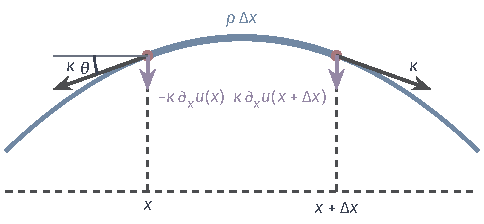
\includegraphics[width=81.975mm]{figures/06-differential-equations/02-partial-differential-equations/tikz/wave-string-element/figure.pdf}
  \caption{弦上一小段$[x,x+\Delta x]$的受力。蓝色粗线是这一小段，质量为$\rho\,\Delta x$。深灰箭头是两端沿切线的张力$\kappa$，紫色箭头是它们的竖直分量。这里弦向上凸，两个竖直分量都向下，合力把这一段拉回平衡位置。}
  \label{fig:wave-string-element}
\end{BookInlineFigure}

右端受到的竖直力是$\kappa\,\partial_xu(x+\Delta x,t)$，左端受到的是$-\kappa\,\partial_xu(x,t)$。再设单位质量上的竖直外力为$f(x,t)$。对这一小段用牛顿第二定律，得到
\[
 \rho\,\Delta x\,\partial_t^{2}u\approx\kappa\bigl[\partial_xu(x+\Delta x,t)-\partial_xu(x,t)\bigr]+\rho\,\Delta x\,f .
\]

两边除以$\rho\,\Delta x$，令$\Delta x\to0$，方括号除以$\Delta x$成为$\partial_x^{2}u$。于是得到一维波动方程：
\begin{equation}
 \partial_t^{2}u=c^{2}\partial_x^{2}u+f,\qquad c^{2}=\frac{\kappa}{\rho}.
 \label{eq:wave-string}
\end{equation}
常数$c>0$称为\term{波速}（wave speed）。量纲上$\kappa/\rho$的单位是$\mathrm{m^2/s^2}$，所以$c$确实是速度，后文会看到它正是扰动传播的速度。例如线密度$0.005\,\mathrm{kg/m}$、张力$80\,\mathrm{N}$的弦，$c=\sqrt{16000}\approx126.5\,\mathrm{m/s}$。张力越大、弦越轻，波跑得越快。

方程中的量各有含义，列在表~\ref{tab:wave-quantities}中。

\begin{BookInlineTable}
  \centering
  \caption{弦振动中各量的含义}
  \label{tab:wave-quantities}
  \begin{tabular}{lll}
    \toprule
    量 & 含义 & 在方程中的作用\\
    \midrule
    $u$ & 竖直位移 & 未知场\\
    $\partial_tu$ & 竖直速度 & 与位移一起构成状态\\
    $\partial_x^{2}u$ & 弦的弯曲 & 决定张力合力\\
    $c$ & 波速 & 把弯曲换算成加速度\\
    $f$ & 单位质量的外力 & 直接提供加速度\\
    \bottomrule
  \end{tabular}
\end{BookInlineTable}

\paragraph{弯曲决定加速度}
式~\eqref{eq:wave-string}和第~\ref{chap:diffusion-equations}章的热方程$\partial_tu=\partial_x^{2}u$右端相同，都是弯曲程度。区别只在左端：弯曲在热方程里决定变化的速度，在波动方程里决定变化的加速度。

这一个差别足以产生完全不同的运动。取初始形状$u_0=\mathrm{e}^{-x^{2}}$，$c=1$，波动问题的初速度为零。在$x=0$处，弯曲是$\partial_x^{2}u_0(0)=-2$。热方程的解在这一点的前期行为是下面左式，波动方程的解是右式：
\[
 u^{\mathrm{heat}}(0,t)\approx1-2t,\qquad u^{\mathrm{wave}}(0,t)\approx1-t^{2}.
\]

热方程中顶点一开始就以速度$2$下降，凡是向上凸的地方都立刻下降，凡是向下凹的地方都立刻上升，所以鼓包被抹平。弦的情形中，同样的弯曲只给出加速度，弦要积累速度才开始移动。一旦有了速度，弯曲消失后运动也不会停下，弦会冲过平衡位置。

图~\ref{fig:wave-curvature-acceleration}把这个差别画了出来。(a)的箭头是弯曲给出的量，(b)中热方程的鼓包逐渐变矮变宽并保持一个峰，(c)中波动方程的鼓包裂成了两个向外移动的峰。

\begin{BookInlineFigure}
  \centering
  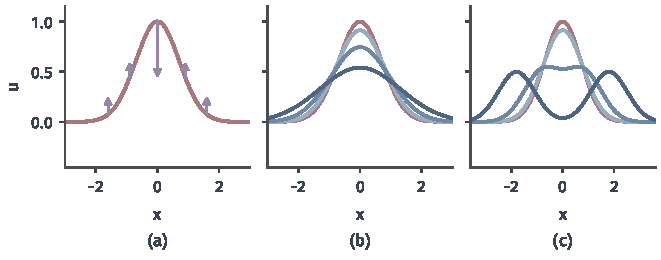
\includegraphics[width=112mm]{figures/06-differential-equations/02-partial-differential-equations/matplotlib/wave-curvature-acceleration/figure.pdf}
  \caption{同样的弯曲，两种后果。(a)初值$\mathrm{e}^{-x^{2}}$（红）和各点的弯曲$\partial_x^{2}u$（紫色箭头）。(b)热方程，蓝色由浅到深为$t=0.05,0.2,0.6$，弯曲作为速度，鼓包被抹平。(c)波动方程，$c=1$，初速度为零，蓝色由浅到深为$t=0.3,0.8,1.8$，弯曲作为加速度，鼓包裂成两个峰。}
  \label{fig:wave-curvature-acceleration}
\end{BookInlineFigure}

\paragraph{把弦看成珠链}
把函数看成很长的向量，可以把这个差别说得更具体。把弦换成$N$颗质量为$\rho h$的珠子，间距为$h$，相邻珠子之间由张力$\kappa$的轻线相连，如图~\ref{fig:wave-bead-chain}。第$j$颗珠子受到两侧的竖直拉力，分别正比于它与邻居的高度差除以$h$。

\begin{BookInlineFigure}
  \centering
  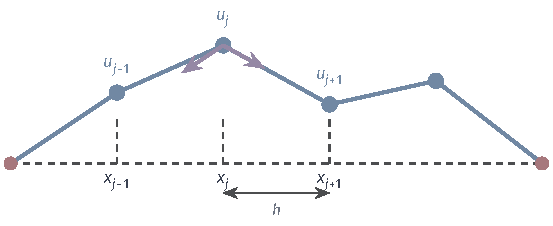
\includegraphics[width=93.606mm]{figures/06-differential-equations/02-partial-differential-equations/tikz/wave-bead-chain/figure.pdf}
  \caption{把弦换成珠链。珠子间距为$h$，两端（红点）固定。第$j$颗珠子受到两侧轻线的拉力（紫色箭头），竖直合力正比于$u_{j+1}-2u_j+u_{j-1}$，这正是二阶差分。}
  \label{fig:wave-bead-chain}
\end{BookInlineFigure}

列出第$j$颗珠子的牛顿第二定律，两端固定时取$u_0=u_{N+1}=0$，并除以质量，得到
\[
 \ddot{u}_j=c^{2}\,\frac{u_{j+1}-2u_j+u_{j-1}}{h^{2}},\qquad j=1,\ldots,N.
\]
记$\bm{u}=(u_1,\ldots,u_N)^\top$，$\bm{K}$为$h^{-2}$乘三对角矩阵$\mathrm{tridiag}(-1,2,-1)$，它对称正定。上式就是
\begin{equation}
 \ddot{\bm{u}}=-c^{2}\bm{K}\bm{u}.
 \label{eq:wave-chain}
\end{equation}

同样的空间离散用在热方程上，得到$\dot{\bm{u}}=-\bm{K}\bm{u}$。两个方程只差一阶时间导数，共用同一个矩阵$\bm{K}$。设$\bm{v}$是$\bm{K}$的特征向量，特征值为$\lambda>0$，把解限制在这个方向上，系数$a(t)$分别满足下面两个常微分方程：
\[
 \dot{a}=-\lambda a,\qquad \ddot{a}=-c^{2}\lambda a.
\]
前者给出衰减$\mathrm{e}^{-\lambda t}$，后者给出振荡$\cos(c\sqrt{\lambda}\,t)$。所以每个方向上一个是指数衰减，一个是不衰减的简谐振动，这是本章反复用到的对应。

这个类比也有失效的地方。珠链的频率有上限，这是因为特征值有上限；连续的弦可以振动得任意快。珠链上的扰动实际上以略低于$c$的速度散开，而连续弦上的波形不变。第~\ref{sec:wave-modes}节会用具体数字比较这些差别，波动方程的离散求解放在第~\ref{chap:pde-numerical-methods}章。

\paragraph{初始状态是一对函数}
式~\eqref{eq:wave-chain}的每个分量都是二阶常微分方程，要同时给位置和速度。连续的弦也一样，初始状态是一对函数：初始位移$u_0$和初始速度$u_1$。第~\ref{chap:pde-problems}章的例子正说明了这一点：$(0,1)$上$c=1$、两端固定时，$\cos(\pi t)\sin(\pi x)$和$(\cos\pi t+\sin\pi t)\sin(\pi x)$的初始位移相同，都是$\sin\pi x$，后续运动却不同。

把区域写成一般形式，本章的问题可以统一写出。

\begin{definition}[波动方程的初边值问题]
\label{def:wave-ibvp}
设$\Omega\subset\mathbb{R}^{d}$为区域，$c>0$，$T>0$。给定源项$f$、初始位移$u_0$和初始速度$u_1$。求$u(\bm{x},t)$满足
\begin{equation}
 \begin{aligned}
  \partial_t^{2}u-c^{2}\Delta u&=f && \text{于}\ \Omega\times(0,T],\\
  u(\cdot,0)=u_0,\quad\partial_tu(\cdot,0)&=u_1 && \text{于}\ \Omega,
 \end{aligned}
 \label{eq:wave-ibvp}
\end{equation}
以及边界$\partial\Omega\times(0,T]$上给定的边界条件。$\Omega=\mathbb{R}^{d}$时没有边界条件。
\end{definition}

\paragraph{端点怎样约束运动}
端点条件有两种基本类型，如图~\ref{fig:wave-boundary-types}。把弦的一端钉死，得到\term{固定端}（fixed end）$u=0$，端点没有位移，因而没有速度。把弦的一端系在一个能沿竖直光滑杆自由滑动的无质量小环上，得到\term{自由端}（free end）。小环在竖直方向不能受力，否则加速度无穷大，所以张力的竖直分量为零，即$\partial_xu=0$。

\begin{BookInlineFigure}
  \centering
  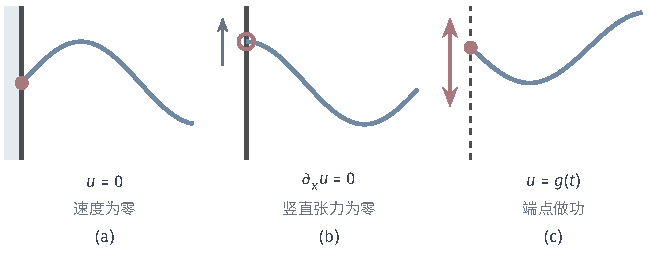
\includegraphics[width=109.703mm]{figures/06-differential-equations/02-partial-differential-equations/tikz/wave-boundary-types/figure.pdf}
  \caption{三种端点。(a)固定端：端点位移和速度为零。(b)自由端：小环沿光滑竖直杆滑动，弦在端点的切线水平。(c)驱动端：端点按给定的位移$g(t)$运动，并通过张力向弦做功。}
  \label{fig:wave-boundary-types}
\end{BookInlineFigure}

两种条件限制的量不同，共同点是端点不向弦输入能量。功率等于力乘速度。在端点上，支撑对弦的竖直力等于$\kappa\,\partial_{\bm{n}}u$，其中$\partial_{\bm{n}}$是外法向导数：右端是$\partial_x$，左端是$-\partial_x$。所以端点向弦输入的功率是
\begin{equation}
 P=\kappa\,\partial_{\bm{n}}u\,\partial_tu .
 \label{eq:wave-end-power}
\end{equation}

固定端让第二个因子$\partial_tu$为零，自由端让第一个因子$\partial_{\bm{n}}u$为零。两种方式都使$P=0$。如果端点按给定的位移运动，或者端点上施加给定的力，式~\eqref{eq:wave-end-power}一般不为零，能量就通过端点进出弦。表~\ref{tab:wave-boundary}总结了这四种情形。

\begin{BookInlineTable}
  \centering
  \caption{端点条件和端点功率}
  \label{tab:wave-boundary}
  \begin{tabular}{llll}
    \toprule
    端点 & 条件 & 被规定的量 & 功率$P$\\
    \midrule
    固定端 & $u=0$ & 位移和速度 & $0$\\
    自由端 & $\partial_{\bm{n}}u=0$ & 竖直力 & $0$\\
    位移驱动 & $u=g(t)$ & 位移和速度 & $\kappa\,\partial_{\bm{n}}u\,g'(t)$\\
    力驱动 & $\kappa\,\partial_{\bm{n}}u=g(t)$ & 竖直力 & $g(t)\,\partial_tu$\\
    \bottomrule
  \end{tabular}
\end{BookInlineTable}

初值和边值在角点处要彼此相容。位移驱动的左端$u(0,t)=g(t)$要有$C^{2}$解，必须满足下面三个条件，它们依次来自位移相等、速度相等和方程在角点处成立：
\[
 u_0(0)=g(0),\qquad u_1(0)=g'(0),\qquad g''(0)=c^{2}u_0''(0)+f(0,0).
\]
固定端是$g\equiv0$的情形。不相容时，间断或折角会从角点出发沿特征线传播，解只能在弱的意义下理解。


\section{一维传播公式}
\label{sec:wave-dalembert}

无界的弦上没有端点干扰，一维波动问题可以完全解出来。解的公式会回答两个问题：初始位移和初始速度各起什么作用，某一时空点的值究竟取决于哪段初值。

\paragraph{换坐标：沿两族直线看}
第~\ref{chap:pde-problems}章指出，一维波动方程的特征线是两族直线$x\pm ct=$常数。沿这两族直线取坐标，方程会变得非常简单。令
\[
 \xi=x-ct,\qquad \eta=x+ct,
\]
并把$u$写成$(\xi,\eta)$的函数。由链式法则，
\[
 \partial_x=\partial_\xi+\partial_\eta,\qquad \partial_t=c(\partial_\eta-\partial_\xi).
\]

把这两个算子分别平方再作差，混合项是唯一留下的部分：
\[
 \partial_t^{2}-c^{2}\partial_x^{2}=c^{2}(\partial_\eta-\partial_\xi)^{2}-c^{2}(\partial_\xi+\partial_\eta)^{2}=-4c^{2}\partial_\xi\partial_\eta .
\]
于是无源的波动方程等价于
\begin{equation}
 \partial_\xi\partial_\eta u=0.
 \label{eq:wave-characteristic-form}
\end{equation}

式~\eqref{eq:wave-characteristic-form}说$\partial_\eta u$不随$\xi$变化，只是$\eta$的函数。对$\eta$积分，积分“常数”是$\xi$的函数。所以$C^{2}$解都可以写成两个一元函数之和：
\begin{equation}
 u(x,t)=F(x-ct)+G(x+ct).
 \label{eq:wave-general-solution}
\end{equation}

$F(x-ct)$是形状$F$以速度$c$向右平移，$G(x+ct)$是形状$G$以速度$c$向左平移。这两项称为\term{行波}（travelling wave）。方程$\partial_t^{2}u=c^{2}\partial_x^{2}u$的全部解都由一列右行波和一列左行波叠加而成，两列波互相穿过，彼此不改变形状。

\paragraph{由初值确定两列波}
把式~\eqref{eq:wave-general-solution}代入两个初始条件，得到
\[
 F(x)+G(x)=u_0(x),\qquad -cF'(x)+cG'(x)=u_1(x).
\]
对第二式从$0$到$x$积分，再除以$c$，其中$K=G(0)-F(0)$是常数：
\[
 G(x)-F(x)=\frac1c\int_0^{x}u_1(s)\,\mathrm{d}s+K .
\]

把它与第一式相加减，就解出了两个函数：
\[
 \begin{aligned}
  F(x)&=\frac12u_0(x)-\frac1{2c}\int_0^{x}u_1(s)\,\mathrm{d}s-\frac K2,\\
  G(x)&=\frac12u_0(x)+\frac1{2c}\int_0^{x}u_1(s)\,\mathrm{d}s+\frac K2 .
 \end{aligned}
\]
代回式~\eqref{eq:wave-general-solution}，常数$K$相消，两个积分合并成从$x-ct$到$x+ct$的积分。这样就得到了下面的公式。

\begin{theorem}[\term{d'Alembert公式}（d'Alembert formula）]
\label{thm:wave-dalembert}
设$u_0\in C^{2}(\mathbb{R})$，$u_1\in C^{1}(\mathbb{R})$。一维问题$\partial_t^{2}u=c^{2}\partial_x^{2}u$，$u(\cdot,0)=u_0$，$\partial_tu(\cdot,0)=u_1$在$\mathbb{R}\times[0,\infty)$上有唯一的$C^{2}$解
\begin{equation}
 u(x,t)=\frac12\bigl[u_0(x-ct)+u_0(x+ct)\bigr]+\frac1{2c}\int_{x-ct}^{x+ct}u_1(s)\,\mathrm{d}s .
 \label{eq:wave-dalembert}
\end{equation}
\end{theorem}

\begin{proof}
先证唯一性。设$u$是$C^{2}$解，换到坐标$(\xi,\eta)$后，$t\geq0$对应区域$\eta\geq\xi$。这个区域在两个坐标方向上的截线都是连通的半直线，所以式~\eqref{eq:wave-characteristic-form}可以如上逐次积分，得到式~\eqref{eq:wave-general-solution}。前面的代入过程说明$F,G$由初值确定到相差一个相消的常数，因此$u$必定是式~\eqref{eq:wave-dalembert}。

再证式~\eqref{eq:wave-dalembert}确实是解。记$x_-=x-ct$，$x_+=x+ct$。由链式法则和变上限积分的求导公式，对$x$求两次，得到
\[
 \partial_x^{2}u=\frac12\bigl[u_0''(x_-)+u_0''(x_+)\bigr]+\frac1{2c}\bigl[u_1'(x_+)-u_1'(x_-)\bigr].
\]

对$t$求一次，$x_\pm$对$t$的导数是$\pm c$，于是
\[
 \partial_tu=\frac c2\bigl[-u_0'(x_-)+u_0'(x_+)\bigr]+\frac12\bigl[u_1(x_+)+u_1(x_-)\bigr].
\]

再对$t$求一次，得到
\[
 \partial_t^{2}u=\frac{c^{2}}2\bigl[u_0''(x_-)+u_0''(x_+)\bigr]+\frac c2\bigl[u_1'(x_+)-u_1'(x_-)\bigr].
\]
比较前后两式，$\partial_t^{2}u=c^{2}\partial_x^{2}u$。题设的光滑性保证这些导数都连续。令$t=0$，$x_-=x_+=x$，积分项为零，$u=u_0$；$\partial_tu$的表达式给出$\partial_tu=u_1$。
\end{proof}

用一组光滑的数据验证公式。取$c=2$，$u_0=\sin x$，$u_1=\cos x$。式~\eqref{eq:wave-dalembert}的两项分别是
\[
 \begin{aligned}
  \frac12\bigl[\sin(x-2t)+\sin(x+2t)\bigr]&=\sin x\cos2t,\\
  \frac14\int_{x-2t}^{x+2t}\cos s\,\mathrm{d}s&=\frac12\cos x\sin2t .
 \end{aligned}
\]
两者之和满足$\partial_t^{2}u=-4u=4\partial_x^{2}u$，$t=0$时位移是$\sin x$，速度是$\cos x$。

式~\eqref{eq:wave-dalembert}有两项，分别来自初始位移和初始速度。由线性性，可以把它们分开讨论。

\paragraph{初始位移的贡献}
取$c=1$，初速度为零，初始位移是帐篷形
\[
 u_0(x)=\Lambda(x)=\max\{1-\lvert x\rvert,\,0\}.
\]
式~\eqref{eq:wave-dalembert}只剩第一项，解是
\begin{equation}
 u(x,t)=\frac12\bigl[\Lambda(x-t)+\Lambda(x+t)\bigr].
 \label{eq:wave-tent-solution}
\end{equation}
帐篷在$0,\pm1$处有折角，严格说来不是$C^{2}$函数，式~\eqref{eq:wave-tent-solution}在折角运动的线上没有二阶导数，它是第~\ref{chap:pde-problems}章意义下的弱解，可以看成光滑初值的解的极限。

式~\eqref{eq:wave-tent-solution}说，初始鼓包分成高度减半的两份，一份向右，一份向左。取$t=1/2$，手算几个点的值：
\[
 \begin{aligned}
  u(0,\tfrac12)&=\tfrac12[\Lambda(-\tfrac12)+\Lambda(\tfrac12)]=\tfrac12,\\
  u(\tfrac12,\tfrac12)&=\tfrac12[\Lambda(0)+\Lambda(1)]=\tfrac12,\\
  u(1,\tfrac12)&=\tfrac12[\Lambda(\tfrac12)+\Lambda(\tfrac32)]=\tfrac14 .
 \end{aligned}
\]
此时两份还重叠着，叠加成高度$1/2$的平台。到$t=1$，两份恰好分开；到$t=2$，它们的中心分别在$\pm2$，中间的弦回到零位，如图~\ref{fig:wave-dalembert-displacement}。

\begin{BookInlineFigure}
  \centering
  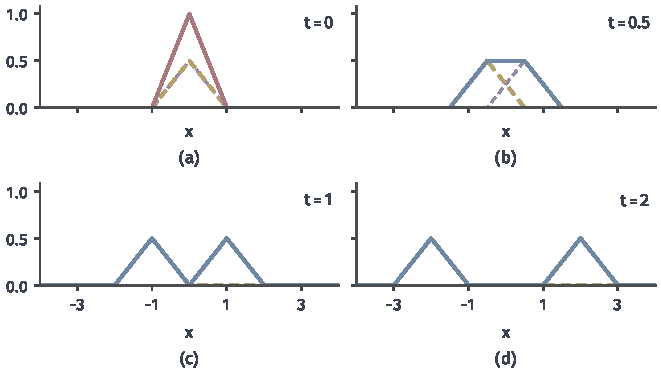
\includegraphics[width=112mm]{figures/06-differential-equations/02-partial-differential-equations/matplotlib/wave-dalembert-displacement/figure.pdf}
  \caption{帐篷形初始位移（$c=1$，初速度为零）在四个时刻的解。黄色虚线是左行波$\frac12\Lambda(x+t)$，紫色虚线是右行波$\frac12\Lambda(x-t)$，实线是两者之和。鼓包分成两半后互不干扰，形状和高度此后不再改变。}
  \label{fig:wave-dalembert-displacement}
\end{BookInlineFigure}

注意帐篷的折角也被带走了。原来的三个折角各分裂成两个，分别沿特征线运动，没有任何一个被磨圆。对比热方程，折角在任意正时刻都消失。波动方程的解在时刻$t$和初值一样光滑，不会更光滑。

\paragraph{初始速度的贡献}
再取初始位移为零，用小锤敲打区间$(-1,1)$，即$c=1$，$u_1=\mathbb{I}\{\lvert x\rvert<1\}$。式~\eqref{eq:wave-dalembert}只剩积分项，被积函数只在$(-1,1)$上不为零，所以
\begin{equation}
 u(x,t)=\frac12\,\bigl\lvert(x-t,\,x+t)\cap(-1,1)\bigr\rvert .
 \label{eq:wave-box-solution}
\end{equation}
竖线表示区间的长度。这个函数连续，但$u_1$的跳跃使它不是$C^{2}$函数，它同样在弱的意义下解方程。

固定一个位置观察。在$x=0$处，式~\eqref{eq:wave-box-solution}的交集在$t\leq1$时是$(-t,t)$，在$t\geq1$时是$(-1,1)$，于是
\[
 u(0,t)=\min\{t,\,1\}.
\]
位移先线性上升，到$t=1$后停在$1$，再也不回来。

固定一个时刻观察。取$t=3$，在几个点上读出交集的长度：
\[
 u(0,3)=\tfrac12\cdot2=1,\qquad u(3,3)=\tfrac12\cdot1=\tfrac12,\qquad u(4,3)=0.
\]
解是一个梯形：在$\lvert x\rvert\leq t-1$上高度为$1$，在$\lvert x\rvert=t+1$处降到零。图~\ref{fig:wave-dalembert-velocity}显示这个梯形不断变宽，高度不变。

\begin{BookInlineFigure}
  \centering
  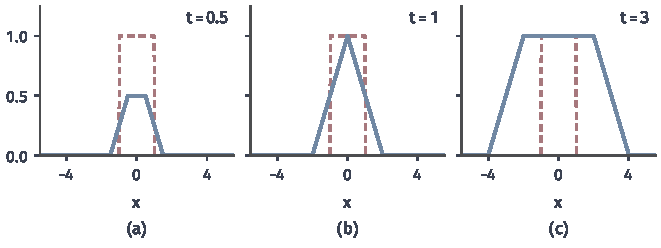
\includegraphics[width=112mm]{figures/06-differential-equations/02-partial-differential-equations/matplotlib/wave-dalembert-velocity/figure.pdf}
  \caption{初始速度为$(-1,1)$的指示函数（红色虚线）时三个时刻的解（蓝），$c=1$，初始位移为零。解是逐渐变宽的梯形，中间的平台高度为$1$，$t>1$后不再升高。}
  \label{fig:wave-dalembert-velocity}
\end{BookInlineFigure}

为什么速度的贡献是积分？设想只在一点$y$附近的小区间$\mathrm{d}y$上有初速度。式~\eqref{eq:wave-dalembert}的积分说，$\lvert x-y\rvert<ct$的点得到位移$u_1(y)\,\mathrm{d}y/(2c)$，更远的点还没有收到信号。一次局部的推动在波前走过的范围内留下固定的抬高，所有$y$的贡献加起来就是积分。

这和初始位移的情形不同。位移的两半走开后，中间恢复零位；速度的作用却留下永久的位移，因为被敲过的弦有净动量。对空间积分可以把这件事算清楚。由式~\eqref{eq:wave-box-solution}，$\int_{\mathbb{R}}\partial_tu\,\mathrm{d}x$保持为初值的积分$2$，所以
\[
 \int_{\mathbb{R}}u(x,t)\,\mathrm{d}x=2t.
\]
梯形的面积正是这样增长的：宽度每单位时间增加$2$，高度为$1$。

\paragraph{一个时空点依赖哪段初值}
式~\eqref{eq:wave-dalembert}直接告诉我们计算$u(x_0,t_0)$要用到什么：$u_0$只用到两个端点$x_0\pm ct_0$，$u_1$用到整个区间$[x_0-ct_0,x_0+ct_0]$。从点$(x_0,t_0)$沿两条特征线回溯到$t=0$，就截出这个区间，如图~\ref{fig:wave-dependence}(a)。

反过来，初值在区间$[a,b]$上的变化只能影响图~\ref{fig:wave-dependence}(b)的阴影区域，$a-ct\leq x\leq b+ct$，以外的点完全不受影响。扰动以速度$c$向两侧扩展。

\begin{BookInlineFigure}
  \centering
  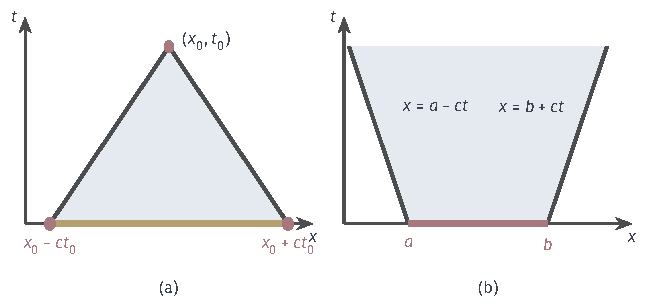
\includegraphics[width=109.647mm]{figures/06-differential-equations/02-partial-differential-equations/tikz/wave-dependence/figure.pdf}
  \caption{一维波动方程的依赖关系。(a)点$(x_0,t_0)$的值由两条特征线（深灰）截出的区间决定：两个红点是所用的位移，黄色线段是所用的速度。(b)初始数据$[a,b]$（红色线段）的变化只能影响阴影区域。}
  \label{fig:wave-dependence}
\end{BookInlineFigure}

用前面的两个例子走一遍。取$c=1$，$(x_0,t_0)=(1/2,2)$，依赖区间是$[-3/2,5/2]$。帐篷初始位移只用到$u_0(-3/2)$和$u_0(5/2)$，两者都为零，于是
\[
 u(\tfrac12,2)=0.
\]
帐篷的两半都已经从这里经过。小锤初始速度要用整个依赖区间，其中包含$(-1,1)$，于是
\[
 u(\tfrac12,2)=\tfrac12\cdot2=1.
\]
如果把初值在$x=3$附近改掉，这两个数都不变，因为$3$不在依赖区间内。

图~\ref{fig:wave-spacetime}把两个例子画在时空平面上。(a)中的折角沿特征线运动，帐篷走后留下空白；(b)中两列波前沿之间的弦保持抬高。

\begin{BookInlineFigure}
  \centering
  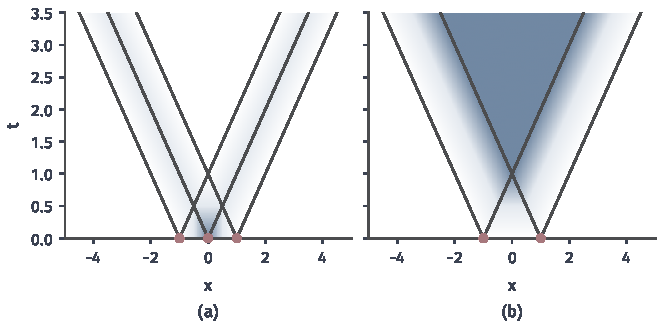
\includegraphics[width=112mm]{figures/06-differential-equations/02-partial-differential-equations/matplotlib/wave-spacetime/figure.pdf}
  \caption{时空平面上的解，$c=1$，颜色越深$u$越大。(a)帐篷形初始位移。(b)$(-1,1)$上的初始速度。深灰直线是从初始数据的折点（红点）出发的特征线，解的不光滑处全部落在这些线上。}
  \label{fig:wave-spacetime}
\end{BookInlineFigure}

\paragraph{解对初值的连续依赖}
由式~\eqref{eq:wave-dalembert}，把两项分别放大，得到点态估计
\begin{equation}
 \sup_{x}\lvert u(x,t)\rvert\leq\sup_{x}\lvert u_0(x)\rvert+t\,\sup_{x}\lvert u_1(x)\rvert .
 \label{eq:wave-sup-bound}
\end{equation}
线性问题中，把它用在两组数据之差上，就得到连续依赖：在有限时间$[0,T]$内，数据的小扰动只造成解的小扰动。

式~\eqref{eq:wave-sup-bound}右端随$t$线性增长，这不是估计不够好。$u_1\equiv1$，$u_0\equiv0$时解是$u=t$，恰好取到等号。这也说明这个估计只在有限时间上有用，长时间的稳定性要另行讨论。

\paragraph{粗糙初值的解}
帐篷和指示函数都不满足定理~\ref{thm:wave-dalembert}的光滑性条件，式~\eqref{eq:wave-dalembert}给出的函数在什么意义下是解？第~\ref{chap:pde-problems}章的回答是弱解：对任意紧支在$\mathbb{R}\times(0,\infty)$中的光滑函数$\varphi$，要求
\begin{equation}
 \iint u\,\bigl(\partial_t^{2}\varphi-c^{2}\partial_x^{2}\varphi\bigr)\,\mathrm{d}x\,\mathrm{d}t=0 .
 \label{eq:wave-weak}
\end{equation}
经典解通过两次分部积分满足它，而式~\eqref{eq:wave-weak}中不再出现$u$的导数。

设$u_0$连续，$u_1$局部可积。取光滑函数列$u_0^{(m)}\to u_0$（在紧集上一致）、$u_1^{(m)}\to u_1$（局部$L^1$），对应的光滑解$u^{(m)}$满足式~\eqref{eq:wave-weak}。把式~\eqref{eq:wave-dalembert}的两项放大，$u^{(m)}$在紧集上一致收敛到由同一公式给出的$u$，于是极限也满足式~\eqref{eq:wave-weak}。这说明$\Lambda$的解和小锤的解是光滑解的极限，式~\eqref{eq:wave-tent-solution}和式~\eqref{eq:wave-box-solution}的说法是合理的。


\section{边界模式}
\label{sec:wave-modes}

弦总有端点，波跑到端点后会怎样？半直线上用反射就能回答，有界区间上波来回反射，解的结构要用模式描述。边界条件决定可用的模式，这一点和第~\ref{chap:diffusion-equations}章相同，时间因子却完全不同。

\paragraph{半直线：固定端的翻转反射}
考虑$x>0$上的弦，端点$x=0$固定。d'Alembert公式需要整条实轴上的数据，我们把初值延拓到$x<0$上，让解自动在$x=0$处为零。如果实轴上的数据关于原点是奇函数，解也是奇函数，因为$-u(-x,t)$满足同样的问题，由唯一性等于$u$；奇函数在$0$处的值只能是$0$。

于是对$u_0,u_1$作\term{奇延拓}（odd extension）：$x<0$时令$u_0(x)=-u_0(-x)$，$u_1(x)=-u_1(-x)$。这是在墙的另一侧放一个翻转的镜像。把延拓后的数据代入式~\eqref{eq:wave-dalembert}，分情况计算。当$x\geq ct$时，$x-ct\geq0$，用不到延拓，公式不变。当$0\leq x<ct$时，$u_0(x-ct)=-u_0(ct-x)$，积分中$(x-ct,\,ct-x)$是对称区间，奇函数的积分为零。

这样就得到半直线固定端的解：
\begin{equation}
 u(x,t)=
 \begin{cases}
  \dfrac12\bigl[u_0(x-ct)+u_0(x+ct)\bigr]+\dfrac1{2c}\displaystyle\int_{x-ct}^{x+ct}u_1\,\mathrm{d}s, & x\geq ct,\\
  \dfrac12\bigl[u_0(ct+x)-u_0(ct-x)\bigr]+\dfrac1{2c}\displaystyle\int_{ct-x}^{ct+x}u_1\,\mathrm{d}s, & 0\leq x<ct .
 \end{cases}
 \label{eq:wave-halfline-fixed}
\end{equation}
第二行中，$-\frac12u_0(ct-x)$是从左侧镜像传来的、已经翻转的反射波。

\paragraph{半直线：自由端的同号反射}
自由端要求$\partial_xu(0,t)=0$。偶函数的导数在$0$处为零，所以改作\term{偶延拓}（even extension）：$u_0(-x)=u_0(x)$，$u_1(-x)=u_1(x)$。镜像不翻转。同样的计算在$0\leq x<ct$时给出
\begin{equation}
 u(x,t)=\frac12\bigl[u_0(ct+x)+u_0(ct-x)\bigr]+\frac1{2c}\Bigl[\int_0^{ct+x}u_1\,\mathrm{d}s+\int_0^{ct-x}u_1\,\mathrm{d}s\Bigr],
 \label{eq:wave-halfline-free}
\end{equation}
$x\geq ct$时仍是式~\eqref{eq:wave-dalembert}。

这两个公式要成为$C^{2}$解，延拓后的数据必须足够光滑。固定端要求$u_0(0)=u_0''(0)=u_1(0)=0$，这正是表~\ref{tab:wave-boundary}之后的相容条件在$g\equiv0$、$f\equiv0$时的结果。自由端要求$u_0'(0)=u_1'(0)=0$。解也是唯一的：若$u$是半直线上固定端的$C^{2}$解，由方程得$\partial_x^{2}u(0,t)=c^{-2}\partial_t^{2}u(0,t)=0$，它的奇延拓在实轴上是$C^{2}$解，再用定理~\ref{thm:wave-dalembert}；自由端用偶延拓同理。

\paragraph{走一遍反射}
取$c=1$，$u_1=0$，初始位移是中心在$x=3$的帐篷$\Lambda(x-3)$。它分成两半，右行的一半直接走开，左行的一半$\frac12\Lambda(x-3+t)$在$t=2$时到达端点，$t=3$时中心位于端点。

在反射发生的时刻，两种端点表现最为不同。取$t=3$，靠近端点$0\leq x\leq1$处的解由式~\eqref{eq:wave-halfline-fixed}和式~\eqref{eq:wave-halfline-free}算出：
\[
 u^{\mathrm{fix}}(x,3)=\tfrac12[\Lambda(x)-\Lambda(-x)]=0,\qquad u^{\mathrm{free}}(x,3)=\Lambda(x).
\]
固定端附近入射波和镜像恰好抵消，位移为零，能量此时全在速度里；自由端附近两者相加，端点位移翻倍，高度达到$1$。

反射之后再取一点比较。在$(x,t)=(1,\,7/2)$处，$ct+x=9/2$，$ct-x=5/2$，代入两个公式：
\[
 u^{\mathrm{fix}}(1,\tfrac72)=\tfrac12[\Lambda(\tfrac32)-\Lambda(-\tfrac12)]=-\tfrac14,\qquad u^{\mathrm{free}}(1,\tfrac72)=\tfrac14 .
\]
固定端反射回来的波被翻转，自由端反射回来的波保持同号，如图~\ref{fig:wave-reflection}。

\begin{BookInlineFigure}
  \centering
  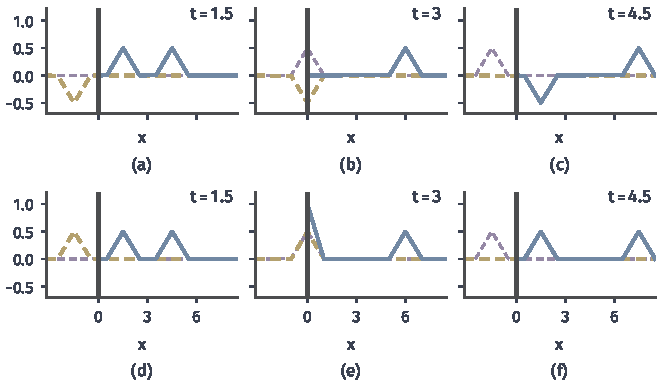
\includegraphics[width=112mm]{figures/06-differential-equations/02-partial-differential-equations/matplotlib/wave-reflection/figure.pdf}
  \caption{半直线上$\Lambda(x-3)$的两半波在端点（深灰竖线）的反射，$c=1$。上排是固定端，下排是自由端。紫色虚线是左行的入射波，黄色虚线是从$x<0$一侧传来的镜像，上排翻转，下排不翻转。蓝线是$x\geq0$上的解，等于两者与右行波之和。}
  \label{fig:wave-reflection}
\end{BookInlineFigure}

\paragraph{区间：分离变量}
现在考虑$(0,L)$上的弦。波在两端之间来回反射，用镜像可以写出来，但更好的办法是换一个角度：寻找形状不变、只有幅度随时间变化的解。设$u(x,t)=X(x)\Theta(t)$，代入$\partial_t^{2}u=c^{2}\partial_x^{2}u$并除以$c^{2}X\Theta$，得到
\[
 \frac{\ddot{\Theta}(t)}{c^{2}\Theta(t)}=\frac{X''(x)}{X(x)}.
\]

左边只依赖$t$，右边只依赖$x$，所以两边等于同一个常数，记作$-\lambda$。这种做法称为\term{分离变量法}（separation of variables）。空间部分是特征值问题，时间部分是简谐振子：
\begin{equation}
 -X''=\lambda X,\qquad \ddot{\Theta}=-c^{2}\lambda\,\Theta .
 \label{eq:wave-separation}
\end{equation}

边界条件落在$X$上。先看两端固定的情形，$X(0)=X(L)=0$。把$X$乘上式并积分，分部积分后边界项为零：
\[
 \lambda\int_0^{L}X^{2}\,\mathrm{d}x=\int_0^{L}(X')^{2}\,\mathrm{d}x .
\]
非零的$X$不可能是常数（它要在端点取零），所以$\lambda>0$。记$\lambda=k^{2}$，$k>0$，通解是$X=A\cos kx+B\sin kx$。条件$X(0)=0$给出$A=0$，条件$X(L)=0$给出$\sin kL=0$，于是
\begin{equation}
 k_n=\frac{n\pi}{L},\qquad X_n(x)=\sin\frac{n\pi x}{L},\qquad n=1,2,\ldots
 \label{eq:wave-dirichlet-modes}
\end{equation}

时间部分的频率是$\omega_n=ck_n=cn\pi/L$，称为第$n$个\term{固有频率}（natural frequency）。

其他端点组合做同样的计算，只是条件换了，结果列在表~\ref{tab:wave-modes}中，前三个模式画在图~\ref{fig:wave-mode-shapes}中。两端自由时多出$\lambda=0$的常数模式，它的时间因子是$a+bt$：整根弦没有受到任何拉回的力，可以整体匀速平移。一端固定一端自由时，$X$在固定端为零、在自由端斜率为零，波长的四分之一装进弦长，所以$k$是$\pi/(2L)$的奇数倍。

\begin{BookInlineTable}
  \centering
  \caption{区间$(0,L)$上三种端点组合的空间模式}
  \label{tab:wave-modes}
  \begin{tabular}{lll}
    \toprule
    端点 & $X_n$ & $k_n$\\
    \midrule
    固定--固定 & $\sin(n\pi x/L)$ & $n\pi/L$，$n\geq1$\\
    自由--自由 & $\cos(n\pi x/L)$ & $n\pi/L$，$n\geq0$\\
    固定--自由 & $\sin((n-\tfrac12)\pi x/L)$ & $(n-\tfrac12)\pi/L$，$n\geq1$\\
    \bottomrule
  \end{tabular}
\end{BookInlineTable}

\begin{BookInlineFigure}
  \centering
  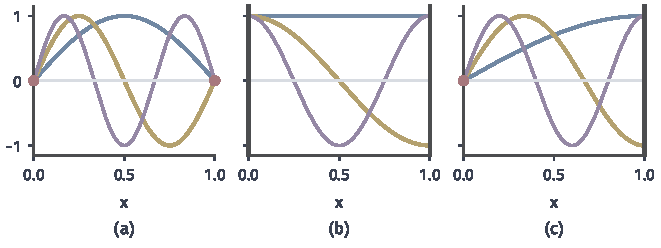
\includegraphics[width=112mm]{figures/06-differential-equations/02-partial-differential-equations/matplotlib/wave-mode-shapes/figure.pdf}
  \caption{$L=1$时的前三个空间模式，蓝、黄、紫依次为$n$增大。红点表示固定端（$X=0$），深灰粗竖线表示自由端（$X'=0$）。(a)固定--固定。(b)自由--自由，蓝线是常数模式。(c)固定--自由。}
  \label{fig:wave-mode-shapes}
\end{BookInlineFigure}

\paragraph{模式展开的解}
两端固定时，由式~\eqref{eq:wave-separation}和线性性，把所有模式叠加起来。把初值按$\sin(n\pi x/L)$展开，系数是
\begin{equation}
 a_n=\frac2L\int_0^{L}u_0(x)\sin\frac{n\pi x}{L}\,\mathrm{d}x,\qquad b_n=\frac2L\int_0^{L}u_1(x)\sin\frac{n\pi x}{L}\,\mathrm{d}x .
 \label{eq:wave-coefficients}
\end{equation}
这组正弦函数在$L^{2}(0,L)$中正交而且完备，这是Fourier级数理论的结果，可参考\BookChapterRef{chap:fourier-transform}{卷四第14章“Fourier变换”}。下面的定理说明，数据足够光滑时级数给出经典解。

\begin{theorem}[两端固定的模式解]
\label{thm:wave-series}
设$u_0\in C^{3}[0,L]$，$u_1\in C^{2}[0,L]$，并满足在$x=0,L$处$u_0=u_0''=0$，$u_1=0$。记$\omega_n=cn\pi/L$，系数由式~\eqref{eq:wave-coefficients}给出，则
\begin{equation}
 u(x,t)=\sum_{n=1}^{\infty}\Bigl(a_n\cos\omega_nt+\frac{b_n}{\omega_n}\sin\omega_nt\Bigr)\sin\frac{n\pi x}{L}
 \label{eq:wave-series}
\end{equation}
是$[0,L]\times[0,\infty)$上的$C^{2}$函数，满足$\partial_t^{2}u=c^{2}\partial_x^{2}u$、两端为零和两个初始条件。
\end{theorem}

\begin{proof}
关键是系数衰减得足够快，使逐项求两次导后的级数一致收敛。记$k_n=n\pi/L$。对$a_n$的积分分部三次：前两次的边界项因$u_0$和$u_0''$在端点为零而消失，第三次仍保留积分。于是
\[
 a_n=-\frac{1}{k_n^{3}}\cdot\frac2L\int_0^{L}u_0'''(x)\cos k_nx\,\mathrm{d}x .
\]

右端的积分是$u_0'''$关于余弦系的系数，由Bessel不等式，这些系数平方可和，所以$(n^{3}a_n)$属于$\ell^{2}$。同样对$b_n$分部两次，$(n^{2}b_n)$属于$\ell^{2}$。由Cauchy--Schwarz不等式，
\[
 \sum_{n}n^{2}\lvert a_n\rvert=\sum_{n}\frac{n^{3}\lvert a_n\rvert}{n}\leq\Bigl(\sum_{n}n^{6}a_n^{2}\Bigr)^{1/2}\Bigl(\sum_{n}\frac1{n^{2}}\Bigr)^{1/2}<\infty,
\]
同理$\sum_nn\lvert b_n\rvert<\infty$。

式~\eqref{eq:wave-series}的通项及其对$x,t$的至多二阶偏导，绝对值都不超过常数乘$n^{2}\lvert a_n\rvert+n\lvert b_n\rvert$。由Weierstrass判别法，这些级数都一致收敛，可以逐项求导，所以$u$是$C^{2}$函数。每一项都满足方程和边界条件，因而$u$也满足。令$t=0$，由余弦和正弦展开的收敛性，得到两个初始条件。
\end{proof}

式~\eqref{eq:wave-series}的解也是唯一的，这要等第~\ref{sec:wave-energy}节用能量证明。数据不够光滑时，只要$(u_0,u_1)\in H_0^{1}(0,L)\times L^{2}(0,L)$，级数仍在能量的意义下收敛，所得的函数是弱解，折线初值就属于这种情形。

自由端的常数模式可以手算验证。取$L=1$，$c=1$，两端自由，$u_0=0$，$u_1=1+\cos\pi x$。把$u_1$看成常数模式和第一个余弦模式之和，常数模式的时间因子是$t$，第一个模式的时间因子是$\sin(\pi t)/\pi$，所以
\[
 u(x,t)=t+\frac{\sin\pi t}{\pi}\cos\pi x .
\]
代入可得
\[
 \partial_t^{2}u=-\pi\sin(\pi t)\cos\pi x=\partial_x^{2}u .
\]
两端$\partial_xu=0$，$t=0$时位移为零，速度是$u_1$。第一项让弦整体匀速上升，第二项是叠加在上面的振动，这是固定端不会出现的现象。

\paragraph{驻波是两列行波之和}
式~\eqref{eq:wave-series}的每一项称为\term{驻波}（standing wave）：形状不变，只是幅度随时间振荡，节点永远不动。这看起来和行波毫无关系。其实由积化和差，
\begin{equation}
 \cos(ckt)\sin(kx)=\frac12\bigl[\sin k(x-ct)+\sin k(x+ct)\bigr].
 \label{eq:wave-standing}
\end{equation}

一个驻波就是一列右行波和一列左行波的叠加，这正是式~\eqref{eq:wave-general-solution}的形式。两列波不断反射，在区间内干涉出固定的形状。图~\ref{fig:wave-standing-traveling}用$L=1$，$c=1$，$n=1$画出了这个分解。

\begin{BookInlineFigure}
  \centering
  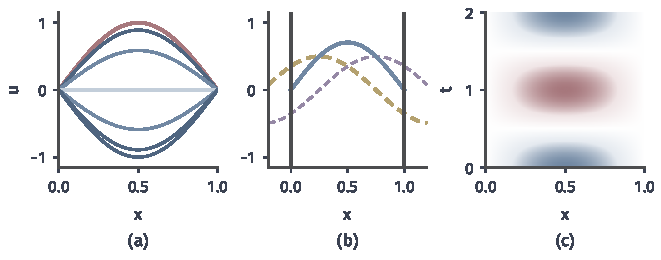
\includegraphics[width=112mm]{figures/06-differential-equations/02-partial-differential-equations/matplotlib/wave-standing-traveling/figure.pdf}
  \caption{第一个驻波$\cos(\pi t)\sin(\pi x)$，$L=1$，$c=1$。(a)不同时刻的形状，红色是$t=0$，端点始终为零。(b)$t=0.25$的分解：黄色虚线是左行波，紫色虚线是右行波，蓝线是两者之和，它在两端（深灰竖线）为零。(c)时空热图，蓝为正，红为负，$t=1$附近弦完全翻转。}
  \label{fig:wave-standing-traveling}
\end{BookInlineFigure}

把这个观察用到整个级数上。对式~\eqref{eq:wave-series}逐项用式~\eqref{eq:wave-standing}，并把$u_0,u_1$作奇延拓后再以$2L$为周期延拓到实轴，得到的正是d'Alembert公式
\begin{equation}
 u(x,t)=\frac12\bigl[\tilde{u}_0(x-ct)+\tilde{u}_0(x+ct)\bigr]+\frac1{2c}\int_{x-ct}^{x+ct}\tilde{u}_1(s)\,\mathrm{d}s .
 \label{eq:wave-interval-extension}
\end{equation}
其中$\tilde{u}_0,\tilde{u}_1$是延拓后的函数。奇延拓保证$x=0$处为零，以$2L$为周期再关于$x=L$也是奇的，所以$x=L$处也为零。这就是在两堵墙之间反复照镜子：反射和模式是同一个解的两种写法。式~\eqref{eq:wave-interval-extension}说明解沿时间有周期$2L/c$，一个波跑到对端再回来刚好用这么长时间。

\paragraph{手算：拨弦的模式}
取$L=1$，$c=1$，初速度为零，把中点拉起成折线$u_0=\min\{x,1-x\}$。由式~\eqref{eq:wave-coefficients}，分部积分后，正弦系数是
\begin{equation}
 a_n=\frac{4}{n^{2}\pi^{2}}\sin\frac{n\pi}{2}.
 \label{eq:wave-pluck-coefficients}
\end{equation}
$n$为偶数时$a_n=0$，这是因为折线关于中点对称，而偶数模式关于中点反对称。前三个非零系数是
\[
 a_1=\frac4{\pi^{2}}\approx0.405,\qquad a_3=-\frac4{9\pi^{2}}\approx-0.045,\qquad a_5=\frac4{25\pi^{2}}\approx0.016 .
\]

解是$u=\sum_na_n\cos(n\pi t)\sin(n\pi x)$。我们用两个时刻核对。在$t=1/2$、$x=1/2$处，奇数$n$的$\cos(n\pi/2)=0$，所以$u(\frac12,\frac12)=0$。用奇周期延拓的d'Alembert公式算，$x\mp t$是$0$和$1$，延拓函数在这两点都是零，结果相同。

在$t=1$时，$\cos(n\pi)=-1$（$n$为奇数），于是$u(x,1)=-u_0(x)$，弦完全翻转。$t=2$时回到初值，运动的周期是$2L/c=2$。图~\ref{fig:wave-plucked-series}的(a)是部分和，三项之后已接近折线，只是尖角处收敛慢；(b)(c)显示折角一直存在，并沿着反射的特征线来回移动。

\begin{BookInlineFigure}
  \centering
  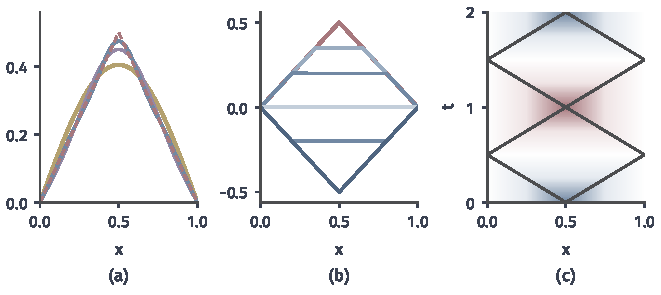
\includegraphics[width=112mm]{figures/06-differential-equations/02-partial-differential-equations/matplotlib/wave-plucked-series/figure.pdf}
  \caption{中点拨起的弦，$L=1$，$c=1$，$u_0=\min\{x,1-x\}$。(a)正弦级数的部分和，黄、紫、蓝分别取到$n=1,3,7$，红色虚线是$u_0$。(b)解的快照，红色是$t=0$，蓝色深浅为$t=0.15,0.3,0.5,0.7,1$，$t=1$时弦完全翻转。(c)时空热图（蓝正红负），深灰折线是在端点反射的特征线，也是折角的轨迹。}
  \label{fig:wave-plucked-series}
\end{BookInlineFigure}

\paragraph{时间因子：振荡与衰减}
同样的空间模式，在第~\ref{chap:diffusion-equations}章的热方程$\partial_tu=\partial_x^{2}u$中，第$n$个模式的时间因子是$\mathrm{e}^{-n^{2}\pi^{2}t}$（$L=1$），在波动方程中是$\cos(n\pi t)$（$c=1$）。图~\ref{fig:wave-heat-mode-factor}并排画出了前三个因子。

热方程的高频模式衰减极快，这就是折角瞬间消失的原因。波动方程的高频模式幅度完全不变，只是振荡得更快。所以波动方程不会平滑初值，初值的高频成分永远留在解里。

\begin{BookInlineFigure}
  \centering
  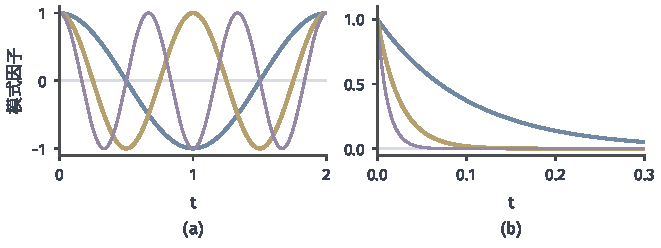
\includegraphics[width=112mm]{figures/06-differential-equations/02-partial-differential-equations/matplotlib/wave-heat-mode-factor/figure.pdf}
  \caption{第$n$个模式的时间因子，$L=1$，蓝、黄、紫依次为$n=1,2,3$。(a)波动方程$\cos(n\pi t)$，$c=1$，幅度不衰减。(b)热方程$\mathrm{e}^{-n^{2}\pi^{2}t}$，模式越高衰减越快（注意时间轴范围不同）。}
  \label{fig:wave-heat-mode-factor}
\end{BookInlineFigure}

\paragraph{离散的模式}
回到式~\eqref{eq:wave-chain}的珠链，看模式如何从有限维走到无限维。设$L=1$，$c=1$，有$N$颗珠子，$h=1/(N+1)$。$\bm{K}$的特征向量正是在格点上取值的$\sin(k\pi x)$，特征值和频率是
\begin{equation}
 \lambda_k=\frac4{h^{2}}\sin^{2}\frac{k\pi h}{2},\qquad \omega_k=\sqrt{\lambda_k}=\frac2h\sin\frac{k\pi h}{2},\qquad k=1,\ldots,N.
 \label{eq:wave-chain-frequencies}
\end{equation}

$N=3$，$h=1/4$时，三个频率和连续弦的$n\pi$比较如下：
\[
 \begin{aligned}
  \text{珠链：}\quad&\omega_1\approx3.06,\quad\omega_2\approx5.66,\quad\omega_3\approx7.39,\\
  \text{连续弦：}\quad&\pi\approx3.14,\quad2\pi\approx6.28,\quad3\pi\approx9.42.
 \end{aligned}
\]
最低的模式已经很准，最高的模式误差最大。图~\ref{fig:wave-discrete-modes}(a)显示珠链的特征向量恰好是连续模式在格点上的采样，(b)显示频率曲线在$N=15$时低端贴合直线$n\pi$，高端向下弯，不能超过$2/h$。这就是第~\ref{sec:wave-problem}节所说类比的失效之处：珠链只有$N$个模式，频率有上限，连续弦的模式无穷多。

\begin{BookInlineFigure}
  \centering
  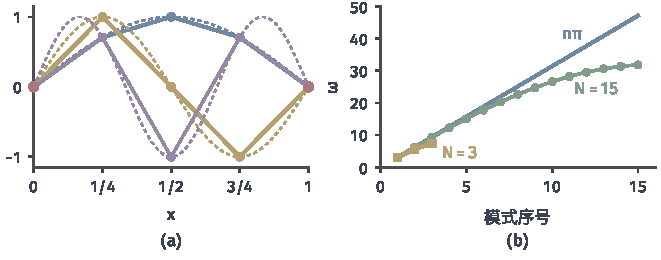
\includegraphics[width=112mm]{figures/06-differential-equations/02-partial-differential-equations/matplotlib/wave-discrete-modes/figure.pdf}
  \caption{珠链和连续弦的模式，$L=1$，$c=1$。(a)$N=3$时的三个特征向量（折线上的点），细虚线是连续模式$\sin(k\pi x)$，红点是固定端。(b)频率随模式序号的变化：蓝线是连续弦$n\pi$，绿线和黄线是$N=15$和$N=3$的珠链。}
  \label{fig:wave-discrete-modes}
\end{BookInlineFigure}


\section{受迫响应}
\label{sec:wave-forced}

弦上持续受力，或者端点被人摇动，解怎样由这些输入决定？线性问题的办法是把输入切成很多瞬时的小份，每一份单独算，再加起来。

\paragraph{脉冲等于初速度}
先看单个振子的例子。第~\ref{chap:linear-differential-systems}章的常数变易公式对$\ddot{x}+\omega^{2}x=g(t)$、零初值给出
\[
 x(t)=\int_0^{t}\frac{\sin\omega(t-s)}{\omega}\,g(s)\,\mathrm{d}s .
\]
被积函数中的$\sin\omega(t-s)/\omega$，是时刻$s$得到单位初速度之后，经过时间$t-s$的自由振动。外力在极短的时间$\mathrm{d}s$内提供的冲量是$g(s)\,\mathrm{d}s$，它的效果就是让速度突然增加这么多。

把振子换成弦，道理不变。时刻$s$的外力$f(\cdot,s)$在$\mathrm{d}s$内给弦增加的速度是$f(\cdot,s)\,\mathrm{d}s$，这相当于在时刻$s$从零位移出发，以这个速度分布开始一次自由振动。

\begin{theorem}[\term{Duhamel原理}（Duhamel's principle）]
\label{thm:wave-duhamel}
设$f$和$\partial_xf$在$\mathbb{R}\times[0,T]$上连续。对每个$s\in[0,T]$，记$w(\cdot,\cdot\,;s)$是自由波动方程在$t\geq s$上的解，它在时刻$s$的位移为零，速度为$f(\cdot,s)$。则
\begin{equation}
 u(x,t)=\int_0^{t}w(x,t;s)\,\mathrm{d}s=\frac1{2c}\int_0^{t}\int_{x-c(t-s)}^{x+c(t-s)}f(y,s)\,\mathrm{d}y\,\mathrm{d}s
 \label{eq:wave-duhamel}
\end{equation}
是$\partial_t^{2}u-c^{2}\partial_x^{2}u=f$在零初值下的$C^{2}$解。
\end{theorem}

\begin{proof}
由式~\eqref{eq:wave-dalembert}，从时刻$s$算起，$w$的表达式为
\[
 w(x,t;s)=\frac1{2c}\int_{x-c(t-s)}^{x+c(t-s)}f(y,s)\,\mathrm{d}y .
\]
它给出式~\eqref{eq:wave-duhamel}的第二个等号。直接求导，$\partial_tw$是$f$在两端点处值的平均，$\partial_t^{2}w$和$\partial_x^{2}w$都由$\partial_xf$在端点的值表示。这些导数对$(x,t,s)$连续，可以在积分号下求导。

对$t$求一次导，积分上限带来一项$w(x,t;t)$。这一项的积分区间长度为零，所以等于零：
\[
 \partial_tu(x,t)=w(x,t;t)+\int_0^{t}\partial_tw(x,t;s)\,\mathrm{d}s=\int_0^{t}\partial_tw(x,t;s)\,\mathrm{d}s .
\]

再求一次导，上限这次带来$\partial_tw(x,t;t)$，按定义它等于$f(x,t)$：
\[
 \partial_t^{2}u=f(x,t)+\int_0^{t}\partial_t^{2}w\,\mathrm{d}s=f(x,t)+c^{2}\int_0^{t}\partial_x^{2}w\,\mathrm{d}s=f+c^{2}\partial_x^{2}u .
\]
令$t=0$，由上面两式得$u(\cdot,0)=0$，$\partial_tu(\cdot,0)=0$。
\end{proof}

定理对$f$的光滑性要求来自$\partial_x^{2}w$要由$\partial_xf$表示。$f$只是连续甚至只是局部可积时，式~\eqref{eq:wave-duhamel}仍有意义，它给出的是弱解，下面持续施力的例子就属于这种情形。一般的初值问题由线性性得到：式~\eqref{eq:wave-dalembert}加上式~\eqref{eq:wave-duhamel}。

\paragraph{外力的依赖区域}
式~\eqref{eq:wave-duhamel}的积分区域是点$(x,t)$的回溯三角形，如图~\ref{fig:wave-duhamel}(a)。时刻$s$的外力只在宽度$2c(t-s)$的切片上起作用，越接近$t$，切片越窄。

三角形内的权重处处是常数$1/(2c)$。换个角度看图~\ref{fig:wave-duhamel}(b)：在点$(y,s)$施加单位脉冲，此后的响应在前向锥内是$1/(2c)$，锥外是零。这是实轴上的Green函数，用公式写是
\begin{equation}
 G(x,t;y,s)=\frac1{2c}\,\mathbb{I}\{\lvert x-y\rvert<c(t-s)\}.
 \label{eq:wave-green}
\end{equation}
式~\eqref{eq:wave-duhamel}就是用$G$对$f$积分。

\begin{BookInlineFigure}
  \centering
  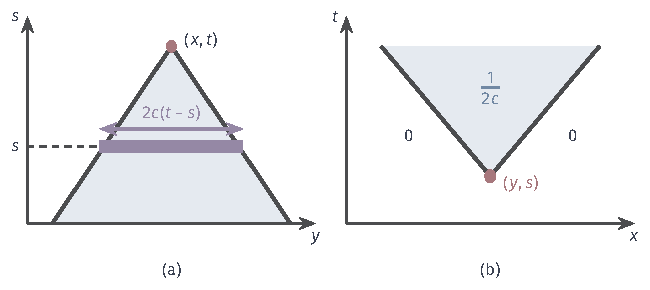
\includegraphics[width=110.06mm]{figures/06-differential-equations/02-partial-differential-equations/tikz/wave-duhamel/figure.pdf}
  \caption{外力的作用范围。(a)计算$u(x,t)$要积分回溯三角形内的$f$，紫色条带是时刻$s$的切片，宽度为$2c(t-s)$。(b)点$(y,s)$（红）的单位脉冲只在前向锥内产生响应，值为$1/(2c)$，锥外为零。}
  \label{fig:wave-duhamel}
\end{BookInlineFigure}

\paragraph{瞬时冲击与持续驱动}
比较两种施力方式，取$c=1$。一种是$t=0$时的一次单位冲击，相当于初速度$\mathbb{I}\{\lvert x\rvert<1\}$，第~\ref{sec:wave-dalembert}节已算出$u(0,t)=\min\{t,1\}$。另一种是在同一区间上持续施力，$f=\mathbb{I}\{\lvert x\rvert<1\}$对所有$t\geq0$成立。

持续驱动相当于每一时刻都敲一次。由式~\eqref{eq:wave-duhamel}，时刻$s$的那一次敲击到$t$时在$x=0$的贡献是$\min\{t-s,1\}$。令$r=t-s$，积分得到
\[
 u(0,t)=\int_0^{t}\min\{r,1\}\,\mathrm{d}r=
 \begin{cases}
  t^{2}/2, & 0\leq t\leq1,\\
  t-\frac12, & t\geq1.
 \end{cases}
\]

例如$t=1$时$u(0,1)=1/2$，$t=3$时$u(0,3)=5/2$。一次冲击的响应到$t=1$后不再变化；持续驱动的响应在$t>1$后线性增长，因为不断有新的敲击的贡献抵达这一点。

图~\ref{fig:wave-impulse-sustained}(a)显示持续驱动如何由各次冲击累加：浅色的梯形是时刻$s=2,1,0$的单次冲击到$t=3$时的响应，蓝色的钟形是所有时刻的积分。(b)是两种情形在原点处的时间历程。

\begin{BookInlineFigure}
  \centering
  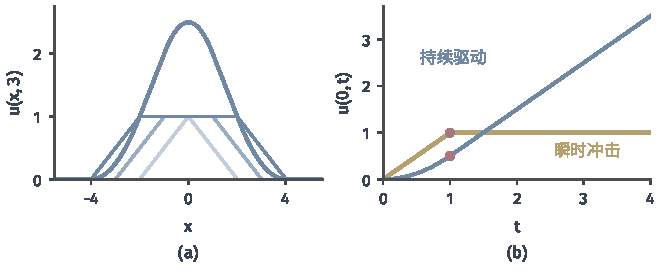
\includegraphics[width=112mm]{figures/06-differential-equations/02-partial-differential-equations/matplotlib/wave-impulse-sustained/figure.pdf}
  \caption{瞬时冲击与持续驱动，$c=1$，力作用在$(-1,1)$上。(a)$t=3$时的位移：蓝色由浅到深的三个梯形是时刻$s=2,1,0$的单次冲击的响应，粗蓝线是持续驱动的解，等于全部冲击响应的积分。(b)原点处的位移，黄线是一次冲击，蓝线是持续驱动，红点是$t=1$时的值$1$和$1/2$。}
  \label{fig:wave-impulse-sustained}
\end{BookInlineFigure}

\paragraph{有限区间：逐模式受迫与共振}
在$(0,L)$上两端固定，把解按式~\eqref{eq:wave-dirichlet-modes}的模式展开，每个系数$a_n(t)$都是一个受迫振子。设$f_n(t)$是$f(\cdot,t)$的正弦系数，零初值时
\begin{equation}
 \ddot{a}_n+\omega_n^{2}a_n=f_n(t),\qquad a_n(t)=\int_0^{t}\frac{\sin\omega_n(t-s)}{\omega_n}f_n(s)\,\mathrm{d}s .
 \label{eq:wave-modal-forcing}
\end{equation}

取$L=1$，$c=1$，$f=\sin(\pi x)\cos(\Omega t)$，只有第一个模式被驱动，固有频率是$\omega_1=\pi$。$\Omega\neq\pi$时，解是特解加上消去初值的齐次解：
\[
 a_1(t)=\frac{\cos\Omega t-\cos\pi t}{\pi^{2}-\Omega^{2}} .
\]
它一直有界。例如$\Omega=2$时，$\lvert a_1\rvert\leq2/(\pi^{2}-4)\approx0.34$。

当$\Omega=\pi$时，上式的分母为零。令$\Omega\to\pi$取极限，由L'Hôpital法则得到
\[
 a_1(t)=\frac{t\sin\pi t}{2\pi} .
\]
代入方程可以验证：$\ddot{a}_1=\cos\pi t-\pi^{2}a_1$。幅度随时间线性增长，这就是共振：外力每个周期都在弦运动的方向上推，能量持续积累。

对比热方程的同一模式。$\dot{a}+\pi^{2}a=\cos\pi t$的解是一个有界的振荡加上快速衰减的暂态，幅度约为$1/(\pi\sqrt{\pi^{2}+1})\approx0.096$。扩散会不断耗掉输入，所以没有共振。图~\ref{fig:wave-resonance}对比了这三种响应。

\begin{BookInlineFigure}
  \centering
  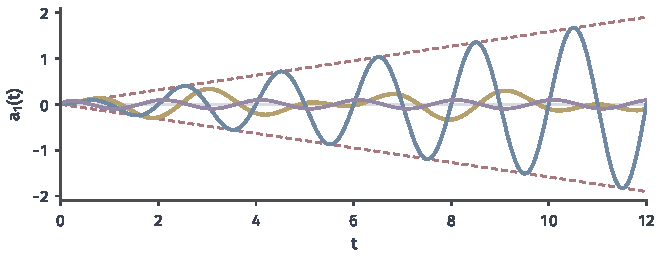
\includegraphics[width=112mm]{figures/06-differential-equations/02-partial-differential-equations/matplotlib/wave-resonance/figure.pdf}
  \caption{第一个模式在外力$\cos\Omega t$下的响应，$L=1$，$c=1$。蓝线是共振$\Omega=\pi$，红色虚线是它的包络$\pm t/(2\pi)$。黄线是非共振$\Omega=2$。紫线是热方程同一模式在$\Omega=\pi$下的响应。}
  \label{fig:wave-resonance}
\end{BookInlineFigure}

\paragraph{边界输入与能量}
除了体内的外力，也可以摇动端点。考虑半直线$x>0$，初值为零，左端按$u(0,t)=g(t)$运动，并设$g(0)=g'(0)=0$。此时右行波$u=g(t-x/c)$满足方程，并在$x=0$处取$g(t)$，所以解是
\begin{equation}
 u(x,t)=
 \begin{cases}
  g(t-x/c), & 0\leq x<ct,\\
  0, & x\geq ct .
 \end{cases}
 \label{eq:wave-boundary-solution}
\end{equation}
端点的运动沿特征线原样传到各处，只是延迟了$x/c$。

由式~\eqref{eq:wave-end-power}，端点的输入要算入能量账。这里$\partial_tu=g'$，$\partial_xu=-g'/c$，端点$x=0$的外法向导数是$-\partial_x$。把$\kappa$换成$c^{2}$（即除以线密度$\rho$），单位质量的输入功率是
\[
 P(t)=c^{2}\cdot\frac{g'(t)}{c}\cdot g'(t)=c\,g'(t)^{2}.
\]
弦原本静止时，摇动端点总在向弦输入能量，功率与端点速度的平方成正比，与$g$的符号无关。

取$c=1$，$g(t)=\sin^{2}\pi t$（$0\leq t\leq1$），此后$g=0$。这里$g'(t)=\pi\sin2\pi t$，$g''$在$t=0,1$有跳跃，所以解的二阶导数在两条特征线$x=t$和$x=t-1$上跳跃，其他位置方程按经典意义成立。累计输入的能量是
\[
 \int_0^{1}P(t)\,\mathrm{d}t=\int_0^{1}\pi^{2}\sin^{2}2\pi t\,\mathrm{d}t=\frac{\pi^{2}}2\approx4.93 .
\]

弦上的能量可以独立算一遍来核对。$t\geq1$时，由式~\eqref{eq:wave-boundary-solution}，$\partial_tu$和$\partial_xu$的平方都等于$g'(t-x)^{2}$，所以
\[
 E(t)=\frac12\int_0^{\infty}\bigl[(\partial_tu)^{2}+(\partial_xu)^{2}\bigr]\,\mathrm{d}x=\int_0^{1}g'(r)^{2}\,\mathrm{d}r=\frac{\pi^{2}}2 .
\]
两种算法结果相同，能量在端点停止摇动后保持不变，如图~\ref{fig:wave-boundary-drive}。

\begin{BookInlineFigure}
  \centering
  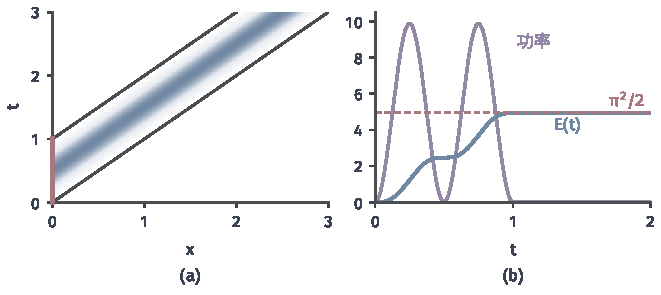
\includegraphics[width=112mm]{figures/06-differential-equations/02-partial-differential-equations/matplotlib/wave-boundary-drive/figure.pdf}
  \caption{端点驱动的半直线，$c=1$，$g(t)=\sin^{2}\pi t$（$0\leq t\leq1$，红色粗线）。(a)时空热图：端点的运动沿特征线传播，深灰直线是波包的前后沿。(b)输入功率$g'(t)^{2}$（紫）和弦上的能量$E(t)$（蓝，由空间积分算出），红色虚线是总输入$\pi^{2}/2$。}
  \label{fig:wave-boundary-drive}
\end{BookInlineFigure}

有限区间上，非齐次的边界条件可以转移成外力。若$u(0,t)=g(t)$，$u(L,t)=0$，令$R(x,t)=g(t)(1-x/L)$，$v=u-R$。$v$在两端为零，满足下面的方程，初值相应地减去$R$和$\partial_tR$在$t=0$的值：
\[
 \partial_t^{2}v-c^{2}\partial_x^{2}v=f-g''(t)\Bigl(1-\frac xL\Bigr).
\]
这样就回到了逐模式受迫的情形。此时端点的功率不一定为正，因为反射回来的波可以推动端点，把能量还给驱动源。


\section{能量估计}
\label{sec:wave-energy}

前面的计算反复出现同一个量：弦的动能加弹性能。不写出解，只对方程乘$\partial_tu$再积分，能得到什么？这样得到的结论不依赖一维公式，也不依赖模式展开，在一般区域上同样成立。

\paragraph{动能和弹性能}
线密度为$\rho$的弦，一小段的动能是$\frac12\rho(\partial_tu)^{2}\,\mathrm{d}x$。弹性能等于张力乘以伸长量，小斜率时一小段的伸长是$\sqrt{1+(\partial_xu)^{2}}\,\mathrm{d}x-\mathrm{d}x\approx\frac12(\partial_xu)^{2}\,\mathrm{d}x$，所以弹性能是$\frac12\kappa(\partial_xu)^{2}\,\mathrm{d}x$。除以$\rho$并推广到$\Omega\subset\mathbb{R}^{d}$，定义\term{动能}（kinetic energy）和\term{弹性能}（elastic energy）之和
\begin{equation}
 E(t)=\frac12\int_\Omega\bigl[(\partial_tu)^{2}+c^{2}\lVert\nabla u\rVert_2^{2}\bigr]\,\mathrm{d}\bm{x}.
 \label{eq:wave-energy}
\end{equation}

\begin{theorem}[能量恒等式]
\label{thm:wave-energy-identity}
设$\Omega\subset\mathbb{R}^{d}$有界，边界分片光滑，$u\in C^{2}(\overline{\Omega}\times[0,T])$满足$\partial_t^{2}u-c^{2}\Delta u=f$。则
\begin{equation}
 E'(t)=\int_\Omega f\,\partial_tu\,\mathrm{d}\bm{x}+c^{2}\int_{\partial\Omega}\partial_tu\,\partial_{\bm{n}}u\,\mathrm{d}S .
 \label{eq:wave-energy-identity}
\end{equation}
特别地，若$f\equiv0$，且边界每一处或者$\partial_tu=0$，或者$\partial_{\bm{n}}u=0$，则$E(t)$为常数。
\end{theorem}

\begin{proof}
积分号下对$t$求导，得到
\[
 E'(t)=\int_\Omega\bigl[\partial_tu\,\partial_t^{2}u+c^{2}\nabla u\cdot\nabla\partial_tu\bigr]\,\mathrm{d}\bm{x}.
\]

第二项用散度定理移走梯度，散度定理的条件和形式可参考\BookChapterRef{chap:integral-theorems}{卷二第27章“积分定理”}：
\[
 \int_\Omega\nabla u\cdot\nabla\partial_tu\,\mathrm{d}\bm{x}=\int_{\partial\Omega}\partial_tu\,\partial_{\bm{n}}u\,\mathrm{d}S-\int_\Omega\partial_tu\,\Delta u\,\mathrm{d}\bm{x}.
\]

代回去，体积分合并成$\int_\Omega\partial_tu(\partial_t^{2}u-c^{2}\Delta u)\,\mathrm{d}\bm{x}$，由方程等于$\int_\Omega f\partial_tu\,\mathrm{d}\bm{x}$。这就是式~\eqref{eq:wave-energy-identity}。无源且边界项为零时，$E'=0$。
\end{proof}

式~\eqref{eq:wave-energy-identity}是能量账：右端第一项是外力的功率，第二项是边界的功率，它正是式~\eqref{eq:wave-end-power}除以$\rho$。固定端、自由端以及给定不随时间变化的位移（此时$\partial_tu=0$）都不进出能量。

\paragraph{和热方程对比}
第~\ref{chap:diffusion-equations}章对热方程也做了能量估计，那里在同样的边界条件下乘的是$u$，得到的是
\[
 \frac{\mathrm{d}}{\mathrm{d}t}\,\frac12\int_\Omega u^{2}\,\mathrm{d}\bm{x}=-\int_\Omega\lVert\nabla u\rVert_2^{2}\,\mathrm{d}\bm{x}\leq0 .
\]
区别在于热方程的能量只含$u$，并且被梯度持续消耗；波动方程的能量同时含$\partial_tu$和$\nabla u$，两部分互相转换，总量不变。这也和两个方程的时间方向性相合：波动方程把$t$换成$-t$仍是波动方程，能量守恒在两个时间方向都成立；热方程只能向前。

\paragraph{手算一个能量账}
继续用中点拨起的弦，$L=1$，$c=1$。$t=0$时速度为零，$\lvert u_0'\rvert=1$几乎处处成立，所以由式~\eqref{eq:wave-energy}，
\[
 E(0)=\frac12\int_0^{1}1\,\mathrm{d}x=\frac12 .
\]

能量也可以按模式计算。把式~\eqref{eq:wave-series}代入式~\eqref{eq:wave-energy}，由三角函数的正交性，不同模式的交叉项为零，每个模式的能量单独守恒：
\begin{equation}
 E=\frac L4\sum_{n=1}^{\infty}\bigl(\omega_n^{2}a_n^{2}+b_n^{2}\bigr).
 \label{eq:wave-modal-energy}
\end{equation}

代入式~\eqref{eq:wave-pluck-coefficients}。只有奇数$n$的项非零，$\omega_n^{2}a_n^{2}=16/(n^{2}\pi^{2})$，于是
\[
 E=\frac14\sum_{n\ \text{奇}}\frac{16}{n^{2}\pi^{2}}=\frac4{\pi^{2}}\sum_{n\ \text{奇}}\frac1{n^{2}}=\frac4{\pi^{2}}\cdot\frac{\pi^{2}}8=\frac12 .
\]
两种算法一致。这里折线初值只是分段光滑，定理~\ref{thm:wave-energy-identity}不能直接用，但式~\eqref{eq:wave-modal-energy}对$H_0^{1}\times L^{2}$的数据仍然成立。第一项占$4/\pi^{2}\approx0.405$，即总能量的$81\%$；加上$n=3$后达$90\%$，加上$n=5$后达$93\%$。高频模式的系数虽小，乘上$\omega_n^{2}$后对能量的贡献并不小。

\paragraph{能量守恒不等于振幅不变}
能量不变，弦上各点的位移却可以大幅变化。回到实轴上的帐篷形初值，由式~\eqref{eq:wave-tent-solution}，$t=0$时能量全是弹性能：
\[
 E=\frac12\int_{-1}^{1}1\,\mathrm{d}x=1,\qquad \max_{x}\lvert u(x,0)\rvert=1.
\]

$t\geq1$时分成两列互不重叠的波，每列的$\partial_tu$和$\partial_xu$的平方都是$1/4$，在长度为$2$的支集上，动能和弹性能都是$\frac12\cdot\frac14\cdot2$，两列相加得到
\[
 K=\frac12,\qquad V=\frac12,\qquad \max_{x}\lvert u(x,t)\rvert=\frac12.
\]
最大位移减半，总能量不变，只是一半的弹性能变成了动能。

图~\ref{fig:wave-energy-accounting}对比了这几种情形。(a)是拨弦的动能和弹性能相互转换，总和恒为$1/2$。(b)是同一初值下热方程的$\frac12\lVert u\rVert_2^{2}$，单调衰减。(c)是实轴上的帐篷，总能量不变，最大位移却下降。

\begin{BookInlineFigure}
  \centering
  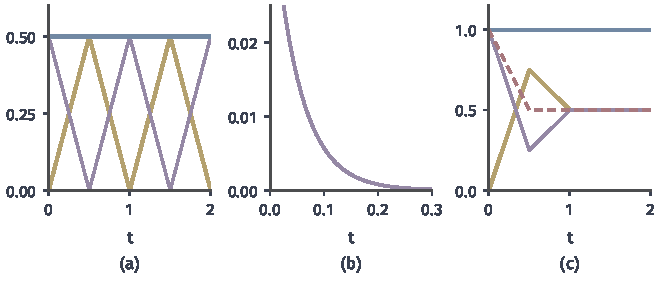
\includegraphics[width=112mm]{figures/06-differential-equations/02-partial-differential-equations/matplotlib/wave-energy-accounting/figure.pdf}
  \caption{能量账。(a)拨弦，$L=1$，$c=1$：黄线是动能，紫线是弹性能，蓝线是两者之和。(b)同一初值在热方程下的$\frac12\lVert u\rVert_2^{2}$（紫），单调下降。(c)实轴上的帐篷：黄、紫、蓝含义同(a)，红色虚线是最大位移，从$1$降到$1/2$，能量却保持为$1$。}
  \label{fig:wave-energy-accounting}
\end{BookInlineFigure}

\paragraph{差解的能量给出唯一性}
能量恒等式最直接的用途是唯一性：设两个解有相同的数据，它们的差的能量从零开始，又不会增加。

\begin{theorem}[唯一性]
\label{thm:wave-uniqueness}
设$\Omega$有界，边界分片光滑。式~\eqref{eq:wave-ibvp}在每一处边界上指定$u$或$\partial_{\bm{n}}u$的条件下，至多有一个$C^{2}(\overline{\Omega}\times[0,T])$解。
\end{theorem}

\begin{proof}
设$u,\tilde{u}$是两个解，$w=u-\tilde{u}$。由线性性，$w$满足无源方程、零初值和齐次的边界条件：在指定$u$的边界上$w=0$，从而$\partial_tw=0$；在指定$\partial_{\bm{n}}u$的边界上$\partial_{\bm{n}}w=0$。定理~\ref{thm:wave-energy-identity}给出$w$的能量为常数，而零初值使它在$t=0$时为零，所以
\[
 \int_\Omega\bigl[(\partial_tw)^{2}+c^{2}\lVert\nabla w\rVert_2^{2}\bigr]\,\mathrm{d}\bm{x}=0,\qquad 0\leq t\leq T.
\]

被积函数连续且非负，所以处处为零，特别地$\partial_tw\equiv0$。于是$w(\bm{x},t)=w(\bm{x},0)=0$。
\end{proof}

边界条件在这里是必需的。在$(0,1)$上取$c=1$，零初值，如果不给边界条件，$u\equiv0$是解，而式~\eqref{eq:wave-boundary-solution}的右行波$g(t-x)$（$g$在$t$很小时为零）也是解：它们的初值相同，差别只来自左端的输入。边界条件正是用来堵住这种能量入口的。

这个证明没有用到解的公式。第~\ref{sec:wave-modes}节的级数解的唯一性由此得到。同样的思路用于有限时间的连续依赖，见下面的增长估计。

\paragraph{外力下的能量增长}
含源项时能量不再守恒，但能估计它增长多快。由式~\eqref{eq:wave-energy-identity}，边界项为零时，Cauchy--Schwarz不等式给出
\[
 E'(t)\leq\lVert f(\cdot,t)\rVert_{L^{2}(\Omega)}\,\lVert\partial_tu(\cdot,t)\rVert_{L^{2}(\Omega)} .
\]

动能不超过总能量，所以$\lVert\partial_tu\rVert_{L^{2}}\leq\sqrt{2E}$，从而
\[
 E'(t)\leq\sqrt2\,\lVert f(\cdot,t)\rVert_{L^{2}(\Omega)}\sqrt{E(t)} .
\]

这种形式的不等式适合对$\sqrt{E}$积分。为了避免$E=0$时除以零，先对$\varepsilon>0$考虑$\sqrt{E+\varepsilon}$，求导后代入上式，得到
\[
 \frac{\mathrm{d}}{\mathrm{d}t}\sqrt{E+\varepsilon}=\frac{E'}{2\sqrt{E+\varepsilon}}\leq\frac1{\sqrt2}\lVert f(\cdot,t)\rVert_{L^{2}(\Omega)} .
\]
积分后令$\varepsilon\to0$，就得到下面的定理。

\begin{theorem}[能量增长估计]
\label{thm:wave-energy-growth}
在定理~\ref{thm:wave-energy-identity}的条件下，设边界项为零。则对$0\leq t\leq T$，
\begin{equation}
 \sqrt{E(t)}\leq\sqrt{E(0)}+\frac1{\sqrt2}\int_0^{t}\lVert f(\cdot,s)\rVert_{L^{2}(\Omega)}\,\mathrm{d}s .
 \label{eq:wave-energy-growth}
\end{equation}
\end{theorem}

用在两组数据的差解上，式~\eqref{eq:wave-energy-growth}给出有限时间内对$(u_0,u_1,f)$的连续依赖，度量是能量范数。

这个估计的增长速度和共振是相合的。继续第~\ref{sec:wave-forced}节的例子，$L=1$，$c=1$，$f=\sin(\pi x)\cos\pi t$。外力的范数和能量分别是
\[
 \lVert f(\cdot,t)\rVert_{L^{2}}=\frac{\lvert\cos\pi t\rvert}{\sqrt2},\qquad E(t)=\frac14\bigl(\dot{a}_1^{2}+\pi^{2}a_1^{2}\bigr),
\]
后者由式~\eqref{eq:wave-modal-energy}对时变系数的同样计算得到。

在$t=12$处，由$a_1=t\sin\pi t/(2\pi)$得$a_1(12)=0$，$\dot{a}_1(12)=6$，所以$\sqrt{E(12)}=3$。式~\eqref{eq:wave-energy-growth}的右端是
\[
 \frac12\int_0^{12}\lvert\cos\pi s\rvert\,\mathrm{d}s=\frac12\cdot12\cdot\frac2\pi=\frac{12}{\pi}\approx3.82 .
\]
上界成立，两者都随$t$线性增长，估计的阶是准确的。如图~\ref{fig:wave-energy-growth}，非共振的$\Omega=2$只让能量有界振荡，这时上界就偏松了：式~\eqref{eq:wave-energy-growth}只用到$\lVert f\rVert_{L^{2}}$，看不到外力和模式频率是否匹配。

\begin{BookInlineFigure}
  \centering
  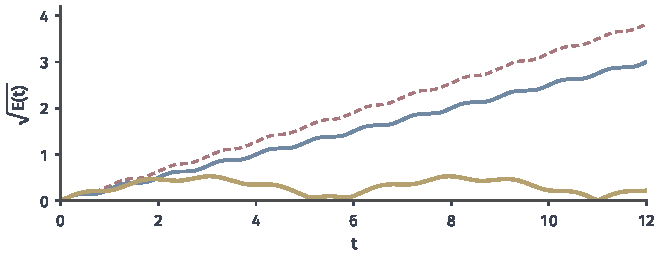
\includegraphics[width=112mm]{figures/06-differential-equations/02-partial-differential-equations/matplotlib/wave-energy-growth/figure.pdf}
  \caption{外力下的$\sqrt{E(t)}$，$L=1$，$c=1$，零初值，$f=\sin(\pi x)\cos\Omega t$。蓝线是共振$\Omega=\pi$，红色虚线是它的上界~\eqref{eq:wave-energy-growth}，两者都线性增长。黄线是非共振$\Omega=2$，能量有界。}
  \label{fig:wave-energy-growth}
\end{BookInlineFigure}


\section{有限传播}
\label{sec:wave-finite-speed}

一维公式告诉我们扰动以速度$c$传播。公式本身不能搬到高维，但这个结论能否脱离公式、在任意维成立？答案是能，用的是把能量局部化到一个收缩的球上。

\paragraph{收缩球上的能量}
设$u$在$\mathbb{R}^{d}$上解无源波动方程。取一点$(\bm{x}_0,t_0)$，考虑以$\bm{x}_0$为中心、半径随时间减小的球：
\[
 B_t=B\bigl(\bm{x}_0,\,c(t_0-t)\bigr),\qquad 0\leq t<t_0 .
\]
这些球叠起来就是顶点在$(\bm{x}_0,t_0)$的\term{传播锥}（propagation cone），如图~\ref{fig:wave-cone-proof}：
\begin{equation}
 K=\bigl\{(\bm{x},t):\lVert\bm{x}-\bm{x}_0\rVert_2\leq c(t_0-t),\ 0\leq t\leq t_0\bigr\}.
 \label{eq:wave-cone}
\end{equation}

直观上，球内的能量有两种变化。一是通过球面的能量通量，它可能把能量带进来；二是球在缩小，边缘上的能量被甩到球外。下面的计算说明，后者足以抵消前者，这恰好需要收缩的速度等于波速。

\begin{BookInlineFigure}
  \centering
  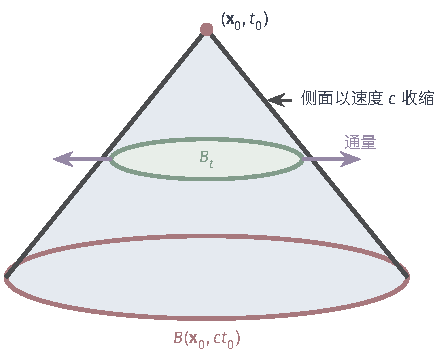
\includegraphics[width=75.406mm]{figures/06-differential-equations/02-partial-differential-equations/tikz/wave-cone-proof/figure.pdf}
  \caption{传播锥。绿色圆盘是时刻$t$的球$B_t$，红色边界是初始的球$B(\bm{x}_0,ct_0)$。紫色箭头是通过球面的能量通量，球的半径以速度$c$减小，通量带来的增量被缩小带走的能量抵消。}
  \label{fig:wave-cone-proof}
\end{BookInlineFigure}

\begin{theorem}[\term{有限传播速度}（finite speed of propagation）]
\label{thm:wave-finite-speed}
设$u\in C^{2}(\mathbb{R}^{d}\times[0,T])$满足$\partial_t^{2}u=c^{2}\Delta u$，$0<t_0\leq T$。若在球$B(\bm{x}_0,ct_0)$上$u_0=u_1=0$，则在传播锥$K$上$u=0$。
\end{theorem}

\begin{proof}
定义局部能量
\[
 e(t)=\frac12\int_{B_t}\bigl[(\partial_tu)^{2}+c^{2}\lVert\nabla u\rVert_2^{2}\bigr]\,\mathrm{d}\bm{x},\qquad 0\leq t<t_0 .
\]
半径变化的球上的积分对$t$求导，除了被积函数的导数，还要加上半径的变化率乘以球面上的积分，这里半径变化率是$-c$。于是
\[
 e'(t)=\int_{B_t}\bigl[\partial_tu\,\partial_t^{2}u+c^{2}\nabla u\cdot\nabla\partial_tu\bigr]\,\mathrm{d}\bm{x}-\frac c2\int_{\partial B_t}\bigl[(\partial_tu)^{2}+c^{2}\lVert\nabla u\rVert_2^{2}\bigr]\,\mathrm{d}S .
\]

和定理~\ref{thm:wave-energy-identity}的证明一样，第一个积分用散度定理和方程化成球面积分，$\bm{n}$为球面的外法向：
\[
 e'(t)=\int_{\partial B_t}\Bigl[c^{2}\partial_tu\,\partial_{\bm{n}}u-\frac c2(\partial_tu)^{2}-\frac{c^{3}}2\lVert\nabla u\rVert_2^{2}\Bigr]\,\mathrm{d}S .
\]

现在估计第一项。法向导数是梯度在单位向量上的分量，所以它的绝对值不超过梯度的范数：
\[
 \lvert\partial_{\bm{n}}u\rvert\leq\lVert\nabla u\rVert_2 .
\]
再对$\lvert\partial_tu\rvert$和$c\lVert\nabla u\rVert_2$用均值不等式：
\[
 c^{2}\lvert\partial_tu\rvert\,\lvert\partial_{\bm{n}}u\rvert\leq c\cdot\lvert\partial_tu\rvert\cdot c\lVert\nabla u\rVert_2\leq\frac c2(\partial_tu)^{2}+\frac{c^{3}}2\lVert\nabla u\rVert_2^{2} .
\]
被积函数因此不超过零，$e'(t)\leq0$。

由假设$e(0)=0$，而$e\geq0$，所以$e(t)=0$对$0\leq t<t_0$成立。于是在$K$内$\partial_tu=0$且$\nabla u=0$。对$K$内任一点$(\bm{x},t)$，线段$\{(\bm{x},s):0\leq s\leq t\}$都在$K$内，沿它积分得$u(\bm{x},t)=u(\bm{x},0)=0$。
\end{proof}

证明中均值不等式的系数恰好是$c/2$，这说明波速$c$是能用的最小收缩速度。球若以更慢的速度收缩，结论就不再成立。取$d=1$，$c=1$，向右传播的帐篷$u=\Lambda(x+5-t)$，支集在$[t-6,t-4]$。$t=0$时支集是$[-6,-4]$，所以$u_0,u_1$在$(-4,4)$上都为零。

让半径按$R(t)=4-t/2$缩小，速度只有$1/2$。这个慢收缩的区间的左端$-R(t)$向右移动得比波包慢，波包追上并进入区间：$t=0$时局部能量为$0$，$t=4$时波包全部在$[-2,0]$内，局部能量等于波包的全部能量$2$。特别地，$u(0,5)=\Lambda(0)=1\neq0$。但这并不违反定理：以$B(0,4)$为底、以速度$1$收缩的锥顶点在$t=4$，点$(0,5)$在锥外。

证明只用到$K$内的方程，所以源项在$K$内为零时结论仍然成立。在有界区域上，只要传播锥不碰到边界，结论就不变；锥碰到固定端或自由端时，边界上的通量项为零，同样的估计在球与$\Omega$的交上仍然有效，端点的影响体现为反射，传播速度依然不超过$c$。

\paragraph{用帐篷核对局部能量}
取$d=1$，$c=1$，帐篷初值，$(x_0,t_0)=(0,3)$，锥在时刻$t$的截面是$\lvert x\rvert\leq3-t$。解$u=F(x-t)+G(x+t)$时，
\[
 (\partial_tu)^{2}+(\partial_xu)^{2}=2F'(x-t)^{2}+2G'(x+t)^{2},
\]
交叉项相消。这里$F=G=\frac12\Lambda$，$\lvert F'\rvert=\frac12$，所以每列波在支集上的能量密度是$\frac12\cdot2\cdot\frac14=\frac14$，长度为$2$，每列带能量$1/2$。

右行波的支集是$[t-1,t+1]$。$t\leq1$时它全在截面内，$e(t)=1$。$t\geq2$时$t-1\geq3-t$，它全部离开截面，$e(t)=0$。$1<t<2$时，留在截面内的长度是$(3-t)-(t-1)=4-2t$，左右两列对称，于是
\begin{equation}
 e(t)=2\cdot\frac14\cdot(4-2t)=2-t,\qquad 1\leq t\leq2.
 \label{eq:wave-local-energy-example}
\end{equation}

这条曲线画在图~\ref{fig:wave-cone-energy}(b)中。局部能量从不增加，波包穿过锥面时能量离开，这正是定理证明中的不等式。(a)是同一过程的时空图。

\begin{BookInlineFigure}
  \centering
  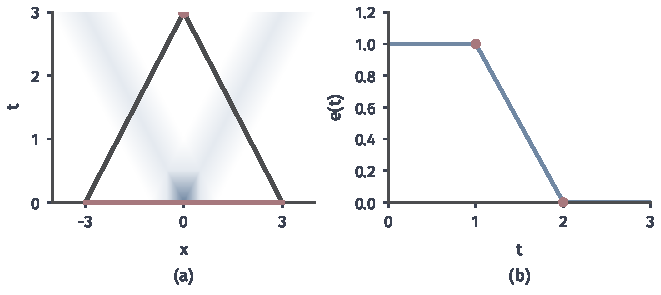
\includegraphics[width=112mm]{figures/06-differential-equations/02-partial-differential-equations/matplotlib/wave-cone-energy/figure.pdf}
  \caption{帐篷解的局部能量，$c=1$，$(x_0,t_0)=(0,3)$。(a)时空图，深灰三角形是传播锥，红色线段是底面。两个波包在$1<t<2$时穿出锥面。(b)由数值积分算出的$e(t)$（蓝），红点标出$t=1,2$，中间一段是式~\eqref{eq:wave-local-energy-example}的直线。}
  \label{fig:wave-cone-energy}
\end{BookInlineFigure}

\paragraph{依赖区域与影响区域}
定理~\ref{thm:wave-finite-speed}可以换一种说法。对线性问题，两个解之差仍是解，所以定理说明：两组初值若在$B(\bm{x}_0,ct_0)$上相同，解在点$(\bm{x}_0,t_0)$的值也相同。这引出下面两个概念。

\begin{definition}[依赖区域与影响区域]
\label{def:wave-domains}
点$(\bm{x}_0,t_0)$的\term{依赖区域}（domain of dependence）是初始时刻的闭球$\overline{B}(\bm{x}_0,ct_0)$。集合$A\subset\mathbb{R}^{d}$的\term{影响区域}（domain of influence）是
\begin{equation}
 \bigl\{(\bm{x},t):t\geq0,\ \mathrm{dist}(\bm{x},A)\leq ct\bigr\}.
 \label{eq:wave-influence}
\end{equation}
\end{definition}

由定理~\ref{thm:wave-finite-speed}，若$u_0,u_1$的支集在$A$内，则$\mathrm{dist}(\bm{x},A)>ct$时$u(\bm{x},t)=0$：以$\bm{x}$为中心、$ct$为半径的球与$A$不相交，初值在球上为零。一维时这两个区域就是图~\ref{fig:wave-dependence}。

定义给出的是“最多”依赖哪些数据，真正依赖的集合可能更小。一维时初始位移只用到两个端点，定理~\ref{thm:wave-finite-speed}无法看出这一点，它只说依赖不会超出球。

\paragraph{与热方程比较}
热方程的解由热核表示。第~\ref{chap:diffusion-equations}章的热核在一维是下面的Gauss函数，$\partial_tu=\partial_x^{2}u$的解是它与初值的卷积：
\[
 \Phi(x,t)=\frac1{\sqrt{4\pi t}}\exp\Bigl(-\frac{x^{2}}{4t}\Bigr),\qquad t>0 .
\]
$\Phi$处处为正，所以非负且不恒为零的初值在任何正时刻都使解处处为正。扰动的“速度”是无穷大的，这和有限传播形成对比。

这个差别需要谨慎理解。取$x=2$，$t=0.01$，单位点源的热核值是
\[
 \Phi(2,0.01)=\frac{\mathrm{e}^{-100}}{\sqrt{0.04\pi}}\approx1.0\times10^{-43},
\]
严格为正，但实际上探测不到。热方程的“无穷速度”是数学结论，物理上是极微弱的尾部。波动方程的前沿外严格为零，不存在尾部。图~\ref{fig:wave-vs-heat-spread}在同一帐篷初值下比较了两者，(c)取对数坐标才看得到热方程的尾部。

\begin{BookInlineFigure}
  \centering
  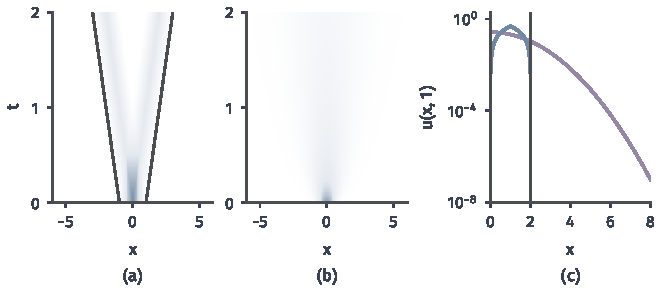
\includegraphics[width=112mm]{figures/06-differential-equations/02-partial-differential-equations/matplotlib/wave-vs-heat-spread/figure.pdf}
  \caption{同一帐篷初值的传播。(a)波动方程（$c=1$）的时空图，深灰线是传播前沿，线外严格为零。(b)热方程（扩散系数为$1$）的时空图，无明确前沿，鼓包逐渐抹平。(c)$t=1$时的对数坐标：紫线是热方程的解，始终为正；蓝线是波动方程的解，到深灰竖线$x=2$处截止。}
  \label{fig:wave-vs-heat-spread}
\end{BookInlineFigure}

\paragraph{耗散与平滑}
除了传播范围，两个方程在耗散和平滑上的差别也来自时间因子。由式~\eqref{eq:wave-pluck-coefficients}，拨弦的第$9$个系数是$a_9=4/(81\pi^{2})\approx0.0050$。$t=0.1$时，$L=1$的两种时间因子分别是
\[
 \mathrm{e}^{-81\pi^{2}\cdot0.1}\approx1.9\times10^{-35},\qquad \cos(0.9\pi)\approx-0.95 .
\]

热方程几乎抹掉了这个模式，波动方程只是改变了它的符号。把所有高频模式放在一起，热方程的解在任意正时刻都是光滑的，波动方程的折角却原样保留，因此逐点的光滑性不可能改善。

反过来，波动方程也没有扩散方程那样的不可逆性。能量不耗散，时间反向后问题仍然适定，高频成分不会在反向时被放大。第~\ref{chap:diffusion-equations}章的逆热问题之所以不稳定，正是因为反向时需要除以极小的因子$\mathrm{e}^{-n^{2}\pi^{2}t}$，而这里的因子模长始终不超过$1$，没有小到需要除的问题。

\paragraph{不要把一维公式搬到高维}
d'Alembert公式依赖换元~\eqref{eq:wave-characteristic-form}，而高维方向不止左右两个，公式没有直接的推广。三维的径向解可以说明这一点。对只依赖$r=\lVert\bm{x}\rVert_2$的函数，$\Delta u=r^{-1}\partial_r^{2}(ru)$，所以$ru$满足一维波动方程。取支集在$(a,b)$内（$a>0$）的光滑函数$\varphi$，外传的球面波是
\begin{equation}
 u(\bm{x},t)=\frac{\varphi(r-ct)}{r} .
 \label{eq:wave-spherical}
\end{equation}
它的幅度按$1/r$衰减，而能量由定理~\ref{thm:wave-energy-identity}（用足够大的球）保持不变：能量摊到越来越大的球面上，每点的振幅自然下降。这比一维行波多了一个衰减因子，是能量守恒与振幅不变并非一回事的另一个例子。

点脉冲的响应在不同维数中的差别更大，如图~\ref{fig:wave-point-response-dimensions}（$c=1$，$t=1$）。一维的响应是$(-1,1)$上的常数$1/2$，前沿过后留下平台。二维的响应在圆盘内是$1/(2\pi\sqrt{1-r^{2}})$，前沿过后留有逐渐衰减的尾巴。三维的响应集中在球面$r=1$上，前沿过后立即归零。这些公式的推导要用到球面平均和降维，篇幅较长，读者可查阅偏微分方程教材。这里要记住的是：前沿之外为零在所有维数中都成立，这是定理~\ref{thm:wave-finite-speed}保证的；前沿之内的形状随维数变化，不能由一维类推。

\begin{BookInlineFigure}
  \centering
  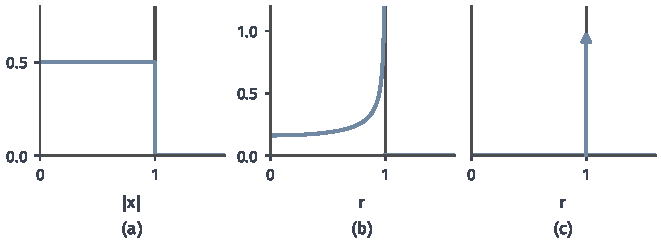
\includegraphics[width=112mm]{figures/06-differential-equations/02-partial-differential-equations/matplotlib/wave-point-response-dimensions/figure.pdf}
  \caption{原点处单位脉冲在$t=1$的响应，$c=1$，横轴为到原点的距离。(a)一维：前沿内是常数$1/2$。(b)二维：前沿内是$1/(2\pi\sqrt{1-r^{2}})$，在$r=1$处发散。(c)三维：全部集中在球面$r=1$上（箭头表示$\delta$分布）。深灰竖线是前沿$r=1$，三种情形在前沿外都为零。}
  \label{fig:wave-point-response-dimensions}
\end{BookInlineFigure}


\section{本章小结}
\label{sec:wave-summary}

本章是椭圆方程和扩散方程之后的补充，讨论二阶时间演化的基本认识。由弦的受力得到波动方程，弯曲决定加速度，所以初始状态是位移和速度一对函数。

一维实轴上，d'Alembert公式把解写成一列右行波和一列左行波。初始位移分成两半走开，初始速度留下不断变宽的平台，依赖区域由两条特征线截出。端点通过反射起作用：固定端翻转，自由端不翻转。

区间上的解按边界条件允许的模式展开，时间因子是不衰减的简谐振动，驻波正是两列行波的叠加。外力用Duhamel原理化成脉冲的叠加，模式频率与外力匹配时出现共振，边界驱动也按功率进入能量账。

表~\ref{tab:wave-summary}对比了扩散方程和波动方程。

\begin{BookInlineTable}
  \centering
  \caption{扩散方程与波动方程的对比}
  \label{tab:wave-summary}
  \begin{tabular}{lll}
    \toprule
    & 扩散方程 & 波动方程\\
    \midrule
    时间阶数 & 一阶 & 二阶\\
    初值 & $u_0$ & $u_0,u_1$\\
    模式因子 & 指数衰减 & 简谐振荡\\
    能量 & $\frac12\lVert u\rVert_2^{2}$单调减小 & 动能加弹性能守恒\\
    传播速度 & 无穷（尾部极弱） & 不超过$c$\\
    折角 & 立即消失 & 沿特征线传播\\
    时间反向 & 不适定 & 适定\\
    外力下 & 无共振 & 共振时线性增长\\
    \bottomrule
  \end{tabular}
\end{BookInlineTable}

能量恒等式不依赖解的公式，由它得到守恒、唯一性和有限时间的增长估计；局部能量进一步给出有限传播速度，在任意维成立。能量守恒不等于振幅不变，前沿之外为零也不说明前沿之内的形状相同，这两点要与一维公式分开理解。

本章只讨论常系数的标量波动方程和有限时间的结论。变系数介质、弹性力学和电磁学中的波动系统，要在具体物理建模需要时，再按一般的双曲系统扩展。


\chapter{输运方程}
\label{chap:transport-equations}

往一条缓缓流动的河里滴一滴墨水。如果忽略墨水向周围的扩散，墨迹只是被水流带着走：水流均匀时，它平移；水流越往下游越快时，它被拉长；水流汇聚时，它被压缩。给定水流的速度，我们想算出此后任意时刻、任意位置的墨水情况。

这个问题的答案取决于“墨水情况”指的是什么。假设每个水粒子带着一个标签，比如颜色的编号，那么粒子走到哪里，标签就带到哪里，数值不变。假设我们关心的是单位长度里有多少墨水，事情就不同了：水流把一段河水拉长一倍，同样多的墨水摊在两倍的长度上，浓度减半。同一个流动，同一个初始形状，这两种量的演化规律不同。

本章先讨论第一种量。沿着粒子的轨迹看，偏微分方程退化成常微分方程，第~\ref{chap:ode-sensitivity}章的流映射正好把初始位置和当前位置联系起来。然后由质量平衡推出第二种量满足的方程，并说明两者的差别恰好来自流动造成的体积变化。

这些构造都依赖足够规则的速度场。最后两节讨论初值带间断时方程应当如何理解，以及数据、源项和速度场的误差怎样影响解。全章速度场都是事先给定的，不受被搬运的量影响。

\section{输运问题}
\label{sec:transp-problem}

先看最简单的情形：一条直河以恒定速度$v$向右流动。用$u(x,t)$表示时刻$t$、位置$x$处水粒子携带的量，比如颜色的深浅。粒子不改变自己携带的值，时刻$t$位于$x$的粒子，在时刻$0$位于$x-vt$，所以
\begin{equation}
  u(x,t)=u_0(x-vt),
  \label{eq:transp-translate}
\end{equation}
其中$u_0$是初始分布。

设$u_0$可微，用链式法则计算式~\eqref{eq:transp-translate}的两个偏导数：
\[
  \partial_tu=-v\,u_0'(x-vt),\qquad \partial_xu=u_0'(x-vt).
\]
第一式加上第二式的$v$倍，右端抵消，得到恒定速度的\term{输运方程}（transport equation）
\begin{equation}
  \partial_tu+v\,\partial_xu=0.
  \label{eq:transp-constant}
\end{equation}

这个方程可以用两种视角读。站在岸上盯住固定位置，$\partial_tu$是看到的变化率：上游的值不断流过来，变化率等于$-v\,\partial_xu$。坐在随水漂流的小船上，周围的水相对自己不动，看到的值不变。式~\eqref{eq:transp-constant}说的就是这两种观察彼此一致。

图~\ref{fig:transp-shift}取$v=1$，初值是以$0$为中心、半宽为$1$的三角形。(a)中三个时刻的曲线形状相同，只是向右平移。(b)把同一个解画在$(x,t)$平面上，颜色的深浅沿斜线$x=x_0+t$保持不变，这些斜线就是粒子的轨迹。

\begin{BookInlineFigure}
  \centering
  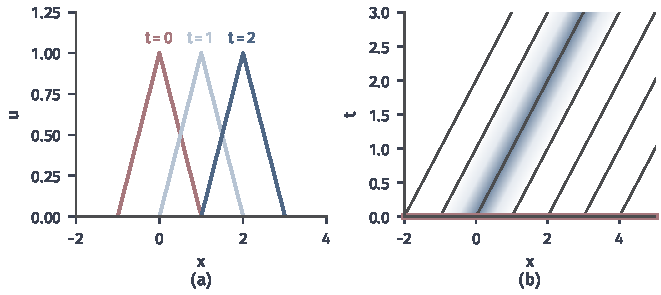
\includegraphics[width=112mm]{figures/06-differential-equations/02-partial-differential-equations/matplotlib/transp-shift/figure.pdf}
  \caption{恒定速度$v=1$的平移。(a)初值（红）和$t=1,2$时的解（蓝色由浅到深）。(b)解$u_0(x-t)$的时空热图，蓝色越深值越大，深灰斜线是粒子轨迹，红线是给定初值的$t=0$。}
  \label{fig:transp-shift}
\end{BookInlineFigure}

水流搬运墨水的比喻有它的边界。真实的墨水还会向四周扩散，边缘逐渐模糊；方程~\eqref{eq:transp-constant}中没有这一项，边缘再陡也不会变缓，初值的尖角和间断都被原样带走。扩散的效果由第~\ref{chap:diffusion-equations}章讨论。

\paragraph{一般的问题}
把水流换成随位置和时间变化的速度场$\bm{v}(\bm{x},t)$，同时允许粒子沿途获得或失去一些量，并考虑有边界的区域，就得到本章要研究的问题。

\begin{definition}[线性输运问题]
\label{def:transp-problem}
设$\Omega\subset\mathbb{R}^{d}$，$\bm{v}:\Omega\times[0,T]\to\mathbb{R}^{d}$是给定的速度场。\term{线性输运问题}（linear transport problem）是求$u(\bm{x},t)$，使
\begin{equation}
  \begin{cases}
    \partial_tu+\bm{v}\cdot\nabla u=f & \text{在}\ \Omega\times(0,T)\ \text{内},\\
    u(\cdot,0)=u_0 & \text{在}\ \Omega\ \text{上},\\
    u=g & \text{在入流边界}\ \Gamma_{-}(t)\ \text{上},
  \end{cases}
  \label{eq:transp-ibvp}
\end{equation}
其中$\bm{n}$是单位外法向，入流边界是
\begin{equation}
  \Gamma_{-}(t)=\{\bm{x}\in\partial\Omega:\bm{v}(\bm{x},t)\cdot\bm{n}(\bm{x})<0\}.
  \label{eq:transp-inflow-boundary}
\end{equation}
当$\Omega=\mathbb{R}^{d}$时，没有边界条件。
\end{definition}

方程中四个已知量的角色不同。
\begin{itemize}
  \item 速度场$\bm{v}$决定粒子往哪里走，它不携带任何场值。
  \item 初始场$u_0$给出时刻$0$在区域内的粒子所携带的值。
  \item 入流数据$g$给出后来从边界进入区域的粒子所携带的值。
  \item 源项$f$描述粒子沿途携带值的变化率，$f=1$表示每个粒子携带的值每单位时间增加$1$。
\end{itemize}

\paragraph{反向追踪}
某个时空点的值由哪些数据决定？从这一点出发，沿粒子的轨迹逆时间往回走，走到已知数据为止。下面以$\Omega=(0,1)$、$v=1/2$为例，此时入流边界只有左端点$x=0$。

如图~\ref{fig:transp-trace}(a)，从$P=(0.8,1)$往回走，轨迹是斜率固定的直线，时间退回$1$时，位置退回$0.5$，到达$(0.3,0)$，落在初始线上。从$Q=(0.2,1)$往回走，在退回时间$0.4$时已到达左端点$(0,0.6)$，落在入流边界上。没有源项时，这两点的值分别是
\[
  u(0.8,1)=u_0(0.3),\qquad u(0.2,1)=g(0.6).
\]

一般地，$(0,1)\times(0,T)$内的点$(x,t)$按下面的方式分成两类，由此得到解的表达式：
\begin{equation}
  u(x,t)=
  \begin{cases}
    u_0(x-vt), & x>vt,\\
    g(t-x/v), & x<vt.
  \end{cases}
  \label{eq:transp-inflow-solution}
\end{equation}
分界线$x=vt$是从角点$(0,0)$出发的轨迹。

\begin{BookInlineFigure}
  \centering
  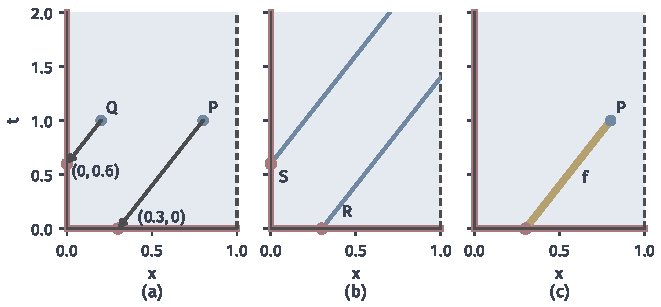
\includegraphics[width=112mm]{figures/06-differential-equations/02-partial-differential-equations/matplotlib/transp-trace/figure.pdf}
  \caption{区间$(0,1)$上$v=1/2$的追踪，红线是给数据的初始线和入流边界，深灰虚线是不给数据的出流边界。(a)从$P,Q$反向追踪到红线上的点。(b)从数据点$R,S$正向出发的影响范围（蓝线）。(c)有源项时，$P$的值还依赖黄色线段上的$f$。}
  \label{fig:transp-trace}
\end{BookInlineFigure}

\paragraph{正向追踪}
反过来，某个数据点影响哪些时空点？从数据点出发沿时间正向走即可。图~\ref{fig:transp-trace}(b)中，从$R$出发的影响范围只有一条线段，这条线段碰到右端点就离开了区域。这与第~\ref{chap:diffusion-equations}章的热方程很不一样，那里一点的扰动瞬间影响全局；与第~\ref{chap:wave-equations}章的波动方程也不同，那里一维的扰动沿左右两条线传播。

\paragraph{源项沿路径累积}
有源项时，粒子沿途不断获得新的量，$P$的值不只依赖轨迹的起点，还依赖整条轨迹上的$f$。如图~\ref{fig:transp-trace}(c)，黄色线段上每一处的$f$都对$u(P)$有贡献，而线段之外的$f$没有影响。这一累积的准确公式在第~\ref{sec:transp-characteristics}节给出。

\paragraph{入流数据与初值的衔接}
式~\eqref{eq:transp-inflow-solution}在分界线$x=vt$的两侧由不同的数据决定，解是否连续取决于角点上的相容性。图~\ref{fig:transp-inflow-solution}比较了两组数据。

(a)中$u_0=\tfrac12(1+\cos2\pi x)$，$g=\cos^{2}(\pi t/2)$。角点上$u_0(0)=g(0)=1$，解沿分界线连续。这里两侧的一阶导数也衔接，因为$u_0'(0)=g'(0)=0$。(b)中$u_0=0$，$g=1$，角点的值不一致，解在分界线上有一个高度为$1$的跳跃，并且这个跳跃沿分界线传播下去，不会被抹平。

\begin{BookInlineFigure}
  \centering
  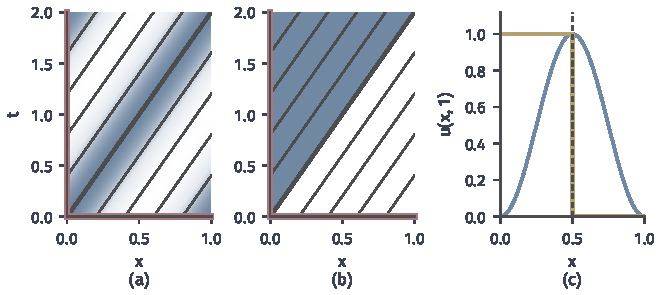
\includegraphics[width=112mm]{figures/06-differential-equations/02-partial-differential-equations/matplotlib/transp-inflow-solution/figure.pdf}
  \caption{$(0,1)$上$v=1/2$的解。(a)初值和入流相容，(b)初值$0$、入流$1$不相容。粗深灰线是分界线$x=t/2$，细深灰线是特征线，红线是给数据的边界，蓝色越深值越大。(c)$t=1$时的剖面，蓝线对应(a)，黄线对应(b)，虚线是分界线的位置。}
  \label{fig:transp-inflow-solution}
\end{BookInlineFigure}

右端点是出流边界，那里的值已由式~\eqref{eq:transp-inflow-solution}确定，不能再独立规定。图~\ref{fig:transp-inflow-solution}(b)的解在$x<t/2$处恒为$1$，在$x>t/2$处恒为$0$，它在分界线上不可导，方程不能逐点成立。这种解的含义留到第~\ref{sec:transp-weak}节讨论。

\section{特征线法}
\label{sec:transp-characteristics}

速度随位置变化时，粒子的轨迹不再是直线，上一节的公式也就不能直接使用。但“坐在小船上看”的想法仍然有效：沿粒子的轨迹求$u$的变化率，偏微分方程会变成常微分方程。

设曲线$\bm{x}(t)$满足$\dot{\bm{x}}=\bm{v}(\bm{x},t)$。沿这条曲线对$u(\bm{x}(t),t)$求导，由链式法则，
\begin{equation}
  \frac{\mathrm{d}}{\mathrm{d}t}u\bigl(\bm{x}(t),t\bigr)
  =\bigl(\partial_tu+\bm{v}\cdot\nabla u\bigr)\bigl(\bm{x}(t),t\bigr).
  \label{eq:transp-along}
\end{equation}
右端正是输运方程的左端。算子$\partial_t+\bm{v}\cdot\nabla$表示跟随粒子时的变化率，称为\term{物质导数}（material derivative）。

\begin{definition}[特征线]
\label{def:transp-characteristic}
设$\bm{v}$是给定的速度场。常微分方程
\begin{equation}
  \dot{\bm{x}}(t)=\bm{v}\bigl(\bm{x}(t),t\bigr)
  \label{eq:transp-char}
\end{equation}
的解$\bm{x}(t)$在时空中的图像$\{(\bm{x}(t),t)\}$称为输运方程的\term{特征线}（characteristic curve）。
\end{definition}

几何上，特征线是时空向量场$(\bm{v},1)$的积分曲线。图~\ref{fig:transp-chardir}中，$(\bm{v},1)$是特征线的切向量，物质导数是$u$沿这个时空方向的方向导数。输运方程规定的只是这一个方向上的导数，其他方向的导数方程不管。这就是沿特征线可以逐条求解的原因。

\begin{BookInlineFigure}
  \centering
  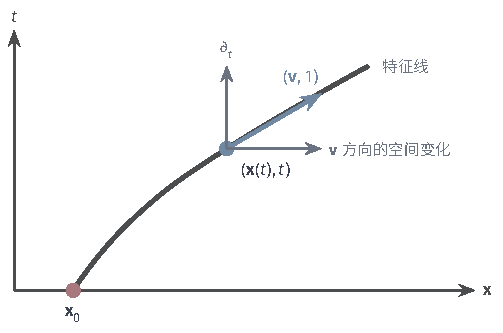
\includegraphics[width=85.2mm]{figures/06-differential-equations/02-partial-differential-equations/tikz/transp-chardir/figure.pdf}
  \caption{时空中的特征线（深灰）。红点是初始位置，蓝色箭头$(\bm{v},1)$是切向量，它由时间方向的一个单位和空间方向的$\bm{v}$合成。物质导数是$u$沿这一方向的方向导数。}
  \label{fig:transp-chardir}
\end{BookInlineFigure}

把偏微分方程沿特征线化为常微分方程，从而逐条求解的方法称为\term{特征线法}（method of characteristics）。

\paragraph{无源输运}
当$f=0$时，式~\eqref{eq:transp-along}说明$u$沿特征线不变。求某点$(\bm{x},t)$的值分三步：解方程~\eqref{eq:transp-char}，得到过这一点的特征线；沿特征线退回到$t=0$，得到出发位置$\bm{x}_0$；令$u(\bm{x},t)=u_0(\bm{x}_0)$。

\begin{example}[均匀拉伸的速度场]
\label{ex:transp-stretch}
取一维速度场$v(x)=x$，初值是以$1$为中心、半宽为$1$的三角形：
\begin{equation}
  u_0(x)=\max\{0,\ 1-\lvert x-1\rvert\}.
  \label{eq:transp-tent}
\end{equation}

特征线满足$\dot{x}=x$，从$x_0$出发的解是
\[
  x(t)=x_0\mathrm{e}^{t}.
\]
反解出发位置，$x_0=x\mathrm{e}^{-t}$。沿特征线$u$不变，于是
\[
  u(x,t)=u_0\bigl(x\mathrm{e}^{-t}\bigr).
\]

在可微的点上代入验证。两个偏导数分别是
\[
  \partial_tu=-x\mathrm{e}^{-t}u_0'\bigl(x\mathrm{e}^{-t}\bigr),\qquad
  x\,\partial_xu=x\mathrm{e}^{-t}u_0'\bigl(x\mathrm{e}^{-t}\bigr),
\]
两者之和为零。

现在算一个具体的点$(x,t)=(3,\ln2)$。特征线的出发位置是$3\mathrm{e}^{-\ln2}=1.5$，所以
\[
  u(3,\ln2)=u_0(1.5)=1-0.5=0.5.
\]
\end{example}

图~\ref{fig:transp-curved}(a)画出了这个例子的特征线。越往右，粒子跑得越快，等间距出发的特征线逐渐散开，解的颜色沿每条特征线不变。(b)是同一个解的剖面：三角形的底从$[0,2]$拉长到$[0,4]$，高度仍然是$1$。(a)中标出的那条特征线把$(1.5,0)$的值$0.5$带到了$(3,\ln2)$，在(b)中对应虚线连接的两点。

\begin{BookInlineFigure}
  \centering
  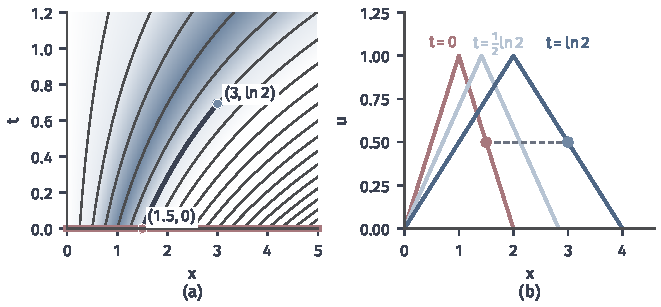
\includegraphics[width=112mm]{figures/06-differential-equations/02-partial-differential-equations/matplotlib/transp-curved/figure.pdf}
  \caption{速度场$v=x$对初值~\eqref{eq:transp-tent}的搬运。(a)特征线$x=x_0\mathrm{e}^{t}$（深灰）和解的时空热图，粗线把$(1.5,0)$（红）连到$(3,\ln2)$（蓝）。(b)初值（红）和$t=\frac12\ln2$、$t=\ln2$的解（蓝色由浅到深），虚线连接同一粒子的前后位置，高度不变。}
  \label{fig:transp-curved}
\end{BookInlineFigure}

速度场显含时间时做法相同，只是特征线的形状要由时间来决定。取$v=\cos t$，特征线$x=x_0+\sin t$来回摆动，解为$u_0(x-\sin t)$。取$v=xt$，特征线是$x=x_0\mathrm{e}^{t^{2}/2}$，解为$u_0(x\mathrm{e}^{-t^{2}/2})$。

图~\ref{fig:transp-timedep}展示了这两种情形。(a)中，每个时刻的速度在空间上处处相同，整个分布作为刚体来回移动。(b)中拉伸的速率随时间增大，特征线弯得越来越厉害。

\begin{BookInlineFigure}
  \centering
  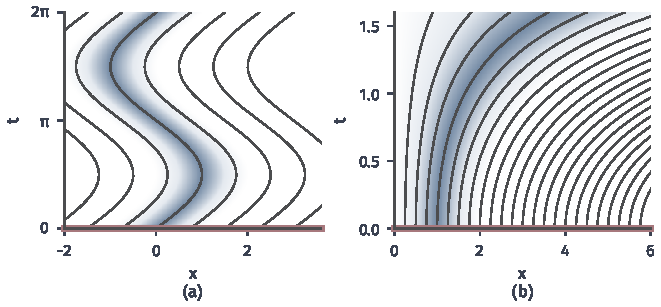
\includegraphics[width=112mm]{figures/06-differential-equations/02-partial-differential-equations/matplotlib/transp-timedep/figure.pdf}
  \caption{显含时间的速度场。深灰线是特征线，蓝色越深值越大，红线是初始线。(a)$v=\cos t$，初值是以$0$为中心、半宽为$1$的三角形。(b)$v=xt$，初值是式~\eqref{eq:transp-tent}。}
  \label{fig:transp-timedep}
\end{BookInlineFigure}

\paragraph{带源项的输运}
有源项时，由式~\eqref{eq:transp-along}，沿特征线的方程变成
\[
  \frac{\mathrm{d}}{\mathrm{d}t}u\bigl(\bm{x}(t),t\bigr)=f\bigl(\bm{x}(t),t\bigr).
\]
右端是沿已知曲线的已知函数，积分即得
\begin{equation}
  u\bigl(\bm{x}(t),t\bigr)=u_0(\bm{x}_0)+\int_0^{t}f\bigl(\bm{x}(s),s\bigr)\,\mathrm{d}s.
  \label{eq:transp-source-along}
\end{equation}
这就是图~\ref{fig:transp-trace}(c)的准确含义：$f$沿轨迹累积到$u$上。

\begin{example}[带源项的计算]
\label{ex:transp-source}
仍取$v=x$与初值~\eqref{eq:transp-tent}，源项取$f(x,t)=x$。沿特征线$x(s)=x_0\mathrm{e}^{s}$，由式~\eqref{eq:transp-source-along}，
\[
  u\bigl(x_0\mathrm{e}^{t},t\bigr)=u_0(x_0)+\int_0^{t}x_0\mathrm{e}^{s}\,\mathrm{d}s=u_0(x_0)+x_0\bigl(\mathrm{e}^{t}-1\bigr).
\]

把$x_0=x\mathrm{e}^{-t}$代回，得到
\[
  u(x,t)=u_0\bigl(x\mathrm{e}^{-t}\bigr)+x\bigl(1-\mathrm{e}^{-t}\bigr).
\]

计算点$(2,\ln2)$。它的出发位置是$x_0=1$，所以
\[
  u(2,\ln2)=u_0(1)+2\cdot\tfrac12=2.
\]
不计源项时，这一点的值是$1$，源项沿特征线累积的贡献是$1$。
\end{example}

图~\ref{fig:transp-source}(b)就是这个累积过程：沿出发于$x_0=1$的特征线，$u$从$1$增长到$\mathrm{e}^{t}$，浅蓝色的面积对应$\int_0^{t}\mathrm{e}^{s}\,\mathrm{d}s$。

\begin{BookInlineFigure}
  \centering
  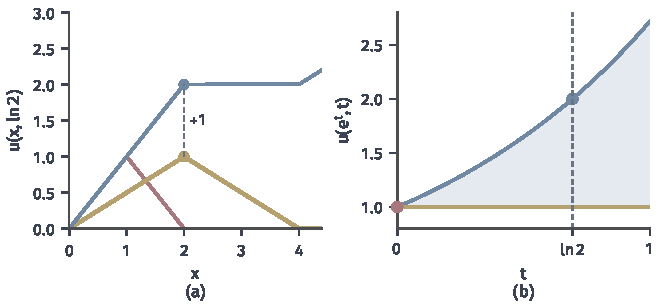
\includegraphics[width=112mm]{figures/06-differential-equations/02-partial-differential-equations/matplotlib/transp-source/figure.pdf}
  \caption{$v=x$、$f=x$的输运。(a)初值（红）、无源解（黄）和有源解（蓝）在$t=\ln2$的剖面，点$x=2$处两解相差$1$。(b)沿特征线$x=\mathrm{e}^{t}$的场值（蓝）与无源时的常值（黄），浅蓝区域是源项的累积，红点是初值。}
  \label{fig:transp-source}
\end{BookInlineFigure}

场的值也可以影响沿途的变化，典型的例子是线性衰减$f=-c(\bm{x},t)\,u+\tilde{f}$。此时沿特征线仍是一个常微分方程，只是变成了线性方程，用积分因子解出：
\begin{equation}
  u\bigl(\bm{x}(t),t\bigr)=\mathrm{e}^{-\int_0^{t}c\,\mathrm{d}r}\,u_0(\bm{x}_0)
  +\int_0^{t}\mathrm{e}^{-\int_s^{t}c\,\mathrm{d}r}\,\tilde{f}\bigl(\bm{x}(s),s\bigr)\,\mathrm{d}s,
  \label{eq:transp-reaction}
\end{equation}
其中$c$沿同一条特征线取值。例如$v=x$，$c=1$，$\tilde{f}=0$时，解为$u=\mathrm{e}^{-t}u_0(x\mathrm{e}^{-t})$。

\paragraph{与经典解的关系}
上面的计算默认了解存在且足够光滑，然后沿特征线推出它的值。这个过程反过来是否成立？按特征线公式造出的函数，是否真的满足方程？这需要速度场和数据的正则性。本章其余部分经常用到下面的条件，这里集中写出。

\medskip
\noindent\textbf{条件（V）.} $\bm{v}:\mathbb{R}^{d}\times[0,T]\to\mathbb{R}^{d}$连续，关于$\bm{x}$连续可微，Jacobian矩阵$\nabla\bm{v}$连续，且存在$L$，使对所有$(\bm{x},t)$有$\lVert\nabla\bm{v}(\bm{x},t)\rVert_2\leq L$。
\medskip

条件（V）说明$\bm{v}$关于$\bm{x}$全局Lipschitz，由第~\ref{chap:ode-existence-continuation}章的整体存在唯一性结论，方程~\eqref{eq:transp-char}过每一点$(\bm{x},t)$恰有一条定义在$[0,T]$上的解，记它在时刻$s$的位置为$\bm{X}(s;\bm{x},t)$。这条解由$\bm{X}(t;\bm{x},t)=\bm{x}$确定。

\begin{theorem}[特征线解与经典解]
\label{thm:transp-classical}
设$\bm{v}$满足条件（V），$u_0\in C^{1}(\mathbb{R}^{d})$，$f$在$\mathbb{R}^{d}\times[0,T]$上连续，关于$\bm{x}$连续可微且$\nabla f$连续。则输运问题~\eqref{eq:transp-ibvp}（$\Omega=\mathbb{R}^{d}$）有唯一的$C^{1}$解，
\begin{equation}
  u(\bm{x},t)=u_0\bigl(\bm{X}(0;\bm{x},t)\bigr)+\int_0^{t}f\bigl(\bm{X}(s;\bm{x},t),s\bigr)\,\mathrm{d}s.
  \label{eq:transp-char-solution}
\end{equation}
\end{theorem}

\begin{proof}
先证唯一性。设$u$是$C^{1}$解。沿过$(\bm{x},t)$的特征线，由式~\eqref{eq:transp-along}和方程，$u$的变化率等于$f$。从$0$到$t$积分，就得到式~\eqref{eq:transp-char-solution}，所以解只能是这个函数。

再证存在性，分两步：先说明这个函数是$C^{1}$的，再验证方程。令
\[
  \bm{\Psi}(\bm{x}_0,t)=\bigl(\bm{X}(t;\bm{x}_0,0),\,t\bigr).
\]
由解对初值的可微性（第~\ref{chap:ode-sensitivity}章），并结合$\partial_t\bm{X}=\bm{v}$，$\bm{\Psi}$是$C^{1}$映射。它的Jacobian矩阵是分块上三角的，对角块分别是$\mathrm{D}_{\bm{x}_0}\bm{X}$和$1$，行列式等于$\det\mathrm{D}_{\bm{x}_0}\bm{X}$，由第~\ref{chap:ode-sensitivity}章的Liouville公式知它恒正。

轨迹唯一性说明$\bm{\Psi}$是$\mathbb{R}^{d}\times[0,T]$到自身的双射。由反函数定理，$\bm{\Psi}^{-1}$也是$C^{1}$的，在$t=0,T$处按单侧导数理解。定义
\[
  W(\bm{x}_0,t)=u_0(\bm{x}_0)+\int_0^{t}f\bigl(\bm{X}(s;\bm{x}_0,0),s\bigr)\,\mathrm{d}s.
\]

$f$关于$\bm{x}$连续可微，所以$W$关于$\bm{x}_0$可以在积分号下求导，并且偏导数连续。$W$关于$t$的偏导数等于被积函数在$s=t$的值，也连续。所以$W\in C^{1}$，从而$u=W\circ\bm{\Psi}^{-1}\in C^{1}$。由于$\bm{X}(s;\bm{x}_0,0)=\bm{X}(s;\bm{x},t)$（同一条特征线），$u$就是式~\eqref{eq:transp-char-solution}的函数。

最后验证方程。由定义，$u(\bm{X}(t;\bm{x}_0,0),t)=W(\bm{x}_0,t)$。对$t$求导，并用式~\eqref{eq:transp-along}，
\[
  \bigl(\partial_tu+\bm{v}\cdot\nabla u\bigr)\bigl(\bm{X}(t;\bm{x}_0,0),t\bigr)=f\bigl(\bm{X}(t;\bm{x}_0,0),t\bigr).
\]
$\bm{\Psi}$是满射，所以方程在每一点成立。$t=0$时，$\bm{X}(0;\bm{x},0)=\bm{x}$，积分为零，初值条件成立。
\end{proof}

条件的作用可以逐一核对。$\bm{v}$的Lipschitz性保证过每点恰有一条特征线，否则“退回到$t=0$”的位置不确定，第~\ref{sec:transp-flow}节会给出具体的反例。$\nabla\bm{v}$的连续性让特征线关于初值$C^{1}$，这是解可微的来源。

$u_0$的$C^{1}$要求不能去掉。例~\ref{ex:transp-stretch}的三角形初值在$x=0,1,2$有折角，公式给出的解沿相应的三条特征线也有折角，它只在这些线之外是经典解。这说明特征线公式可以比方程本身走得更远，第~\ref{sec:transp-weak}节用测试函数解释这种解。有界区域的情形要把积分的下限换成特征线离开区域的时刻，并要求初值和入流数据在角点上按第~\ref{sec:transp-problem}节的方式衔接。

\section{流映射}
\label{sec:transp-flow}

上一节一次只跟踪一条特征线。把所有特征线放在一起看，固定两个时刻，每个粒子从前一时刻的位置走到后一时刻的位置，这就是一个空间到自身的映射。第~\ref{chap:ode-sensitivity}章已经研究过它，这里把要用的结论写下来。

\paragraph{流映射回顾}
对速度场$\bm{v}$，流映射$\bm{\varphi}_{s,t}(\bm{x})$表示时刻$s$位于$\bm{x}$的粒子在时刻$t$的位置，即
\begin{equation}
  \partial_t\bm{\varphi}_{s,t}(\bm{x})=\bm{v}\bigl(\bm{\varphi}_{s,t}(\bm{x}),t\bigr),\qquad
  \bm{\varphi}_{s,s}(\bm{x})=\bm{x}.
  \label{eq:transp-flow}
\end{equation}
上一节的$\bm{X}(s;\bm{x},t)$就是$\bm{\varphi}_{t,s}(\bm{x})$。

在条件（V）下，$\bm{\varphi}_{s,t}$是$\mathbb{R}^{d}$到自身的$C^{1}$双射。第~\ref{chap:ode-sensitivity}章还给出了两条代数规则：走两段等于走一段，走过去再走回来回到原处，即
\begin{equation}
  \bm{\varphi}_{r,t}\circ\bm{\varphi}_{s,r}=\bm{\varphi}_{s,t},\qquad
  \bm{\varphi}_{t,s}=\bm{\varphi}_{s,t}^{-1}.
  \label{eq:transp-flow-rules}
\end{equation}

\paragraph{输运解的表示}
用流映射重写式~\eqref{eq:transp-char-solution}，得到
\begin{equation}
  u(\cdot,t)=u_0\circ\bm{\varphi}_{t,0}+\int_0^{t}f(\cdot,s)\circ\bm{\varphi}_{t,s}\,\mathrm{d}s.
  \label{eq:transp-flow-solution}
\end{equation}
这里出现的是逆向的映射$\bm{\varphi}_{t,0}$。粒子带着值$u_0(\bm{x}_0)$从$\bm{x}_0$走到$\bm{\varphi}_{0,t}(\bm{x}_0)$，要想知道固定位置$\bm{y}$的值，必须先问“现在位于$\bm{y}$的粒子原来在哪里”，然后到初值里去查。

图~\ref{fig:transp-lookup}把例~\ref{ex:transp-stretch}的三个粒子连了起来。这时$\varphi_{0,\ln2}(x)=2x$，上下两条曲线上用箭头相连的点高度相同。要读下面的曲线在$y=3$处的值，就从$y=3$沿箭头退回$x_0=1.5$，到上面的曲线上读出$0.5$。

\begin{BookInlineFigure}
  \centering
  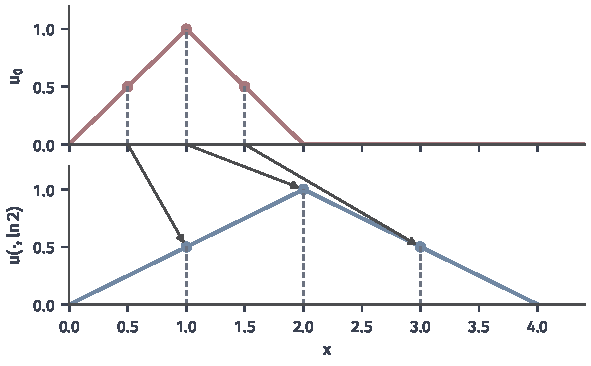
\includegraphics[width=100mm]{figures/06-differential-equations/02-partial-differential-equations/matplotlib/transp-lookup/figure.pdf}
  \caption{用流映射搬运场值，$v=x$，$t=\ln2$。上图是初值（红），下图是搬运后的解（蓝）。箭头把位置$x_0=0.5,1,1.5$连到$2x_0$，点的高度保持不变。}
  \label{fig:transp-lookup}
\end{BookInlineFigure}

同一个解有两种描述方式。跟着粒子看，$u(\bm{\varphi}_{0,t}(\bm{x}_0),t)=u_0(\bm{x}_0)$，这称为\term{Lagrange描述}（Lagrangian description），标号是粒子的初始位置。站在固定位置看，$u(\bm{y},t)=u_0(\bm{\varphi}_{t,0}(\bm{y}))$，这称为\term{Euler描述}（Eulerian description），标号是当前位置。两者用流映射互相转换，这也是公式中需要逆映射的原因。

$v=x$时流映射是$\varphi_{s,t}(x)=x\mathrm{e}^{t-s}$。规则~\eqref{eq:transp-flow-rules}在这里就是指数的相加。$v=xt$时流映射依赖两个时刻：
\[
  \varphi_{s,t}(x)=x\exp\Bigl(\frac{t^{2}-s^{2}}{2}\Bigr).
\]
这时$\varphi_{0,1}$的倍数是$\mathrm{e}^{1/2}$，$\varphi_{1,2}$的倍数是$\mathrm{e}^{3/2}$，相乘得到$\varphi_{0,2}$的倍数$\mathrm{e}^{2}$，符合式~\eqref{eq:transp-flow-rules}；但第二段时间的倍数不等于第一段，同样长的时间间隔走出的倍数不同，所以必须记住起止两个时刻。

平面上的情形类似。旋转场$\bm{v}=(-x_2,x_1)^{\top}$的流映射是旋转矩阵，鞍点场$\bm{v}=(x_1,-x_2)^{\top}$沿一个方向拉伸，沿另一个方向压缩：
\[
  \bm{\varphi}_{t}^{\mathrm{rot}}(\bm{x})=
  \begin{pmatrix}\cos t&-\sin t\\ \sin t&\cos t\end{pmatrix}\bm{x},\qquad
  \bm{\varphi}_{t}^{\mathrm{sad}}(\bm{x})=
  \begin{pmatrix}\mathrm{e}^{t}&0\\ 0&\mathrm{e}^{-t}\end{pmatrix}\bm{x}.
\]

图~\ref{fig:transp-2d-advect}用式~\eqref{eq:transp-flow-solution}搬运了一个由两团组成的初值。旋转把它转了四分之一圈，形状不变；鞍点流把它在一个方向拉长、另一个方向压扁。两种情形下，解的最大值都和初值相同，因为$u$只是被搬动，没有哪个粒子携带的值发生了变化。

\begin{BookInlineFigure}
  \centering
  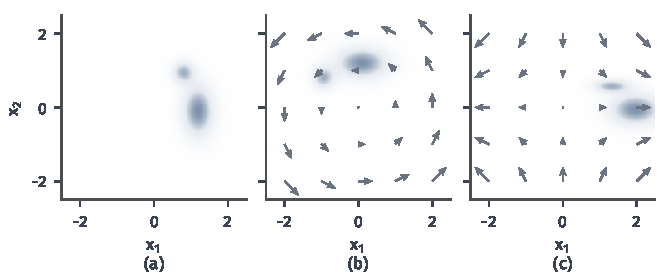
\includegraphics[width=112mm]{figures/06-differential-equations/02-partial-differential-equations/matplotlib/transp-2d-advect/figure.pdf}
  \caption{平面上的搬运，蓝色越深值越大，三幅图共用一个色阶，灰色箭头是速度场的方向。(a)初值。(b)旋转场，$t=\pi/2$。(c)鞍点场$\bm{v}=(x_1,-x_2)^{\top}$，$t=0.5$。}
  \label{fig:transp-2d-advect}
\end{BookInlineFigure}

\paragraph{逆映射的范围}
条件（V）保证了粒子不会在有限时间内跑到无穷远，也就保证了$\bm{\varphi}_{s,t}$在全空间上定义。去掉全局Lipschitz条件后，轨迹可能爆炸，逆映射的定义域就受到限制。

取$v=x^{2}$，第~\ref{chap:ode-sensitivity}章已经算出它的流映射：
\[
  \varphi_{0,t}(x)=\frac{x}{1-tx},\qquad x<\frac1t\quad(t>0).
\]
当$x$跑遍$(-\infty,1/t)$时，$\varphi_{0,t}(x)$跑遍$(-1/t,\infty)$。于是从初始线出发的粒子在时刻$t$只占据$y>-1/t$，反解得到的逆映射只在这个范围内有定义：
\[
  \varphi_{t,0}(y)=\frac{y}{1+ty},\qquad y>-\frac1t.
\]

图~\ref{fig:transp-flow-domain}(a)中，浅红色区域$\{x\leq-1/t\}$里的点没有来自初始线的特征线，它们的值由初值无法确定，这些特征线要追溯到“从$-\infty$进来”。另一方面，$x_0\geq1/t$的粒子在时刻$t$之前已经跑到了$+\infty$。例如$(y,t)=(1,1)$的出发位置是$1/2$，而$(y,t)=(-2,1)$没有出发位置。

\begin{BookInlineFigure}
  \centering
  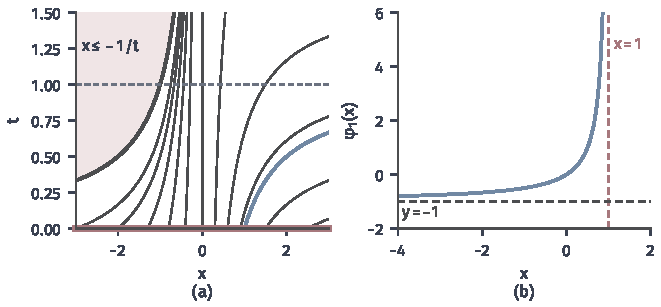
\includegraphics[width=112mm]{figures/06-differential-equations/02-partial-differential-equations/matplotlib/transp-flow-domain/figure.pdf}
  \caption{速度场$v=x^{2}$的流映射只在部分区域可逆。(a)特征线（深灰），蓝线是从$x_0=1$出发、在$t=1$爆炸的轨迹，粗深灰线$x=-1/t$是从初始线可达区域的边界，浅红区域无法追溯到初始线。(b)$\varphi_{0,1}(x)=x/(1-x)$，定义在$x<1$，值域是$(-1,\infty)$。}
  \label{fig:transp-flow-domain}
\end{BookInlineFigure}

所以一般情形下，式~\eqref{eq:transp-flow-solution}只在点$(\bm{y},t)$的反向轨迹能够回到$t=0$时才有意义。这时解存在的区域是流映射的值域，而不是整个时空。

\paragraph{轨迹唯一性}
即使轨迹全局存在，失去唯一性也会破坏这种表示。取$v(x)=2\sqrt{\lvert x\rvert}$，它在$x=0$处不Lipschitz。从负轴出发的粒子向右运动，在有限时间到达$0$，然后可以在$0$停留任意一段时间，再离开。过$(0,c)$向右离开的轨迹是$x=(t-c)^{2}$。

看图~\ref{fig:transp-nonunique}(a)中的点$P=(1,2)$。反向追踪得到$x=(r-1)^{2}$，在$r=1$到达$0$。再往回，有多条轨迹都能走到$(0,1)$：可以一直停在$0$，也可以来自负轴。凡是出发位置$x_0\in[-1,0]$的粒子，都可能在时刻$2$到达$P$，图中用红色粗线标出这些出发位置，黄色虚线是其中两条。

如果$u$是$C^{1}$解，它沿每条这样的轨迹都不变，所以$u_0$在$[-1,0]$上必须是常数。只要初值在这一段上不是常数，方程就没有$C^{1}$解。

\begin{BookInlineFigure}
  \centering
  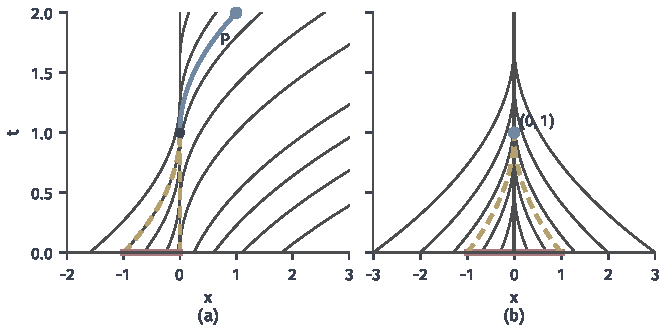
\includegraphics[width=112mm]{figures/06-differential-equations/02-partial-differential-equations/matplotlib/transp-nonunique/figure.pdf}
  \caption{速度场不Lipschitz时的轨迹。(a)$v=2\sqrt{\lvert x\rvert}$，轨迹在$x=0$处分叉，蓝线是到达$P$的最后一段，黄色虚线是到达$(0,1)$的两条路径，红色粗线是可能的出发位置$[-1,0]$。(b)$v=-2\,\mathrm{sgn}(x)\sqrt{\lvert x\rvert}$，轨迹并入$x=0$，从蓝点反向追踪的出发位置是红色粗线$[-1,1]$。}
  \label{fig:transp-nonunique}
\end{BookInlineFigure}

图~\ref{fig:transp-nonunique}(b)是反方向的情形。$v=-2\,\mathrm{sgn}(x)\sqrt{\lvert x\rvert}$下，粒子都流向$0$，正向轨迹是唯一的，但$[-1,1]$中的粒子在$t=1$时都已并入$0$，$\varphi_{0,1}$不是单射，逆映射不存在。从$(0,1)$反向追踪得到一整段出发位置，$u_0$在$[-1,1]$上不是常数时，同样不存在$C^{1}$解。

这两个例子说明，输运解的表示依赖于$\bm{\varphi}_{s,t}$的可逆性，可逆性又依赖轨迹在正反两个方向上的唯一性。以下都假设条件（V），需要讨论局部情形时，会明确说明定义域。


\section{连续性方程}
\label{sec:transp-continuity}

回到例~\ref{ex:transp-stretch}。三角形被$v=x$搬运到$t=\ln2$时，底变成了原来的两倍，高度不变，曲线下的面积从$1$变成了$2$。如果$u$表示粒子携带的标签，这没有问题；如果用它表示单位长度的墨水质量，总质量就凭空翻了一倍。质量不会凭空产生，所以墨水的浓度不满足输运方程，我们需要一个由质量平衡出发的新方程。

\paragraph{一维的质量平衡}
用$\rho(x,t)$表示单位长度的质量，取一段固定的区间$[a,b]$。流量$\rho v$是单位时间穿过某一点的质量，正号表示向右。如图~\ref{fig:transp-balance}(a)，区间内质量的变化等于从$a$流入的减去从$b$流出的，再加上区间内的源项$f$：
\[
  \frac{\mathrm{d}}{\mathrm{d}t}\int_a^{b}\rho\,\mathrm{d}x
  =\rho v\big|_{x=a}-\rho v\big|_{x=b}+\int_a^{b}f\,\mathrm{d}x.
\]

设$\rho$、$v$足够光滑，用微积分基本定理把两端的差写成积分：
\[
  \int_a^{b}\bigl(\partial_t\rho+\partial_x(\rho v)-f\bigr)\,\mathrm{d}x=0.
\]
区间是任取的，被积函数连续，所以它恒为零，这就是一维的连续性方程。

\begin{BookInlineFigure}
  \centering
  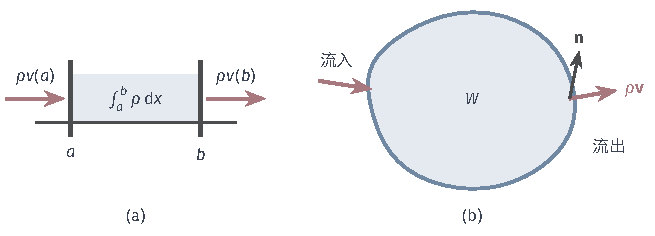
\includegraphics[width=111mm]{figures/06-differential-equations/02-partial-differential-equations/tikz/transp-balance/figure.pdf}
  \caption{控制区域的质量平衡。(a)区间$[a,b]$内的质量变化由两端的流量差决定。(b)平面区域$W$，红色箭头是质量流$\rho\bm{v}$，它在外法向$\bm{n}$上的投影为正时流出、为负时流入。}
  \label{fig:transp-balance}
\end{BookInlineFigure}

\paragraph{多维的质量平衡}
取固定的\term{控制区域}（control region）$W\subset\mathbb{R}^{d}$，如图~\ref{fig:transp-balance}(b)，边界光滑。穿过边界的质量流是$\rho\bm{v}\cdot\bm{n}$，于是
\begin{equation}
  \frac{\mathrm{d}}{\mathrm{d}t}\int_W\rho\,\mathrm{d}\bm{x}
  =-\int_{\partial W}\rho\bm{v}\cdot\bm{n}\,\mathrm{d}S+\int_Wf\,\mathrm{d}\bm{x}.
  \label{eq:transp-balance}
\end{equation}
由散度定理（见\BookChapterRef{chap:integral-theorems}{卷二第27章“积分定理”}），边界积分等于$\int_W\nabla\cdot(\rho\bm{v})\,\mathrm{d}\bm{x}$。由$W$的任意性，得到下面的方程。

\begin{definition}[连续性方程]
\label{def:transp-continuity}
给定速度场$\bm{v}$和源项$f$，未知密度$\rho(\bm{x},t)$满足的方程
\begin{equation}
  \partial_t\rho+\nabla\cdot(\rho\bm{v})=f
  \label{eq:transp-continuity}
\end{equation}
称为\term{连续性方程}（continuity equation）。
\end{definition}

把散度展开，可以看清它与输运方程的差别：
\begin{equation}
  \partial_t\rho+\bm{v}\cdot\nabla\rho=f-\rho\,\nabla\cdot\bm{v}.
  \label{eq:transp-divergence-correction}
\end{equation}
左端仍然是物质导数，右端多了一项$-\rho\nabla\cdot\bm{v}$，它就是散度修正。粒子携带的值不变，但$\rho$是“粒子周围的拥挤程度”，流动把周围的空间撑大或压小，这个量就要变。

当$\nabla\cdot\bm{v}=0$时修正项消失，两个方程完全一样，这样的速度场称为\term{无散度速度场}（divergence-free velocity field）。一般的速度场下两个方程不同，同一个初值走出的结果也不同。

\begin{example}[同一流动下的值与密度]
\label{ex:transp-rho-stretch}
仍取$v=x$，初值同式~\eqref{eq:transp-tent}。连续性方程是式~\eqref{eq:transp-reaction}的$c=\nabla\cdot v=1$情形，沿特征线的解是
\[
  \rho(x,t)=\mathrm{e}^{-t}\rho_0\bigl(x\mathrm{e}^{-t}\bigr).
\]

直接代入验证。对$t$求偏导，
\[
  \partial_t\rho=-\mathrm{e}^{-t}\rho_0-x\mathrm{e}^{-2t}\rho_0'.
\]
$\partial_x(x\rho)=\rho+x\partial_x\rho$，其中第一项是$\mathrm{e}^{-t}\rho_0$，第二项是$x\mathrm{e}^{-2t}\rho_0'$。两式相加为零。

点$(3,\ln2)$的出发位置是$1.5$。输运方程的解是$u(3,\ln2)=0.5$，连续性方程的解是
\[
  \rho(3,\ln2)=\tfrac12\cdot\rho_0(1.5)=0.25.
\]

积分验证总量。三角形的面积是$1$，时刻$t$时，对$\rho$换元$z=x\mathrm{e}^{-t}$，
\[
  \int_{\mathbb{R}}\rho(x,t)\,\mathrm{d}x=\int_{\mathbb{R}}\rho_0(z)\,\mathrm{d}z=1.
\]
同样的换元用在$u$上，多出的因子$\mathrm{e}^{t}$没有抵消，于是$\int u(x,t)\,\mathrm{d}x=\mathrm{e}^{t}$。
\end{example}

图~\ref{fig:transp-value-density}把这个例子放在一起比较。(a)和(b)的初值、流动完全相同，(a)中三角形的高度不变，面积翻倍；(b)中高度减半，面积不变。(c)是沿$x_0=1$这条特征线的三个量：$u$恒为$1$，体积倍率$J=\mathrm{e}^{t}$增长，密度$\rho=\mathrm{e}^{-t}$下降，乘积$\rho J$恒为$1$。

\begin{BookInlineFigure}
  \centering
  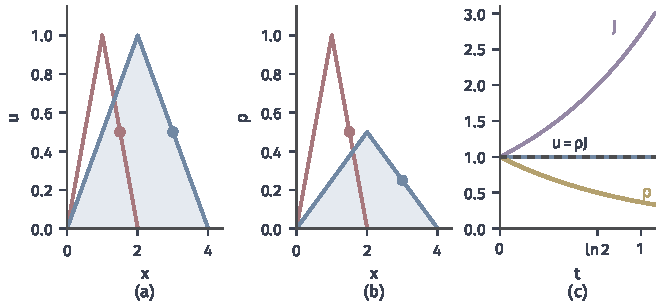
\includegraphics[width=112mm]{figures/06-differential-equations/02-partial-differential-equations/matplotlib/transp-value-density/figure.pdf}
  \caption{$v=x$，$t=\ln2$，初值同式~\eqref{eq:transp-tent}（红）。(a)场值$u$，浅蓝面积为$2$。(b)密度$\rho$，浅蓝面积为$1$，两图中的点都是$x_0=1.5$及其像。(c)沿$x_0=1$的特征线：$u$（蓝）、$\rho$（黄）、体积倍率$J$（紫）与乘积$\rho J$（虚线）。}
  \label{fig:transp-value-density}
\end{BookInlineFigure}

这里有两件容易混淆的事。沿轨迹密度不变，说的是物质导数为零，这只在$\nabla\cdot\bm{v}=0$时成立；总质量不变，说的是全空间的积分不随时间变化，它在$\bm{v}$不是无散度时同样成立，只要密度衰减足够快、没有质量从边界流失。例~\ref{ex:transp-rho-stretch}中总质量不变，沿轨迹的密度却在下降。

\subsection{体积变化}
\label{sec:transp-volume}

修正项$\rho\nabla\cdot\bm{v}$的来历，要从体积的变化说起。想象一维流动中相邻的两个粒子，相距$\Delta x$。前面的粒子比后面的多走了$\bigl(v(x+\Delta x)-v(x)\bigr)\,\mathrm{d}t$，所以它们的间距以$\partial_xv\,\Delta x$的速度增大，相对增长率就是$\partial_xv$。散度是这个现象在多维的写法。

\paragraph{Jacobian的演化}
记流映射的Jacobian行列式
\begin{equation}
  J_{s,t}(\bm{x})=\det\mathrm{D}\bm{\varphi}_{s,t}(\bm{x}).
  \label{eq:transp-jacobian}
\end{equation}

第~\ref{chap:ode-sensitivity}章证明了，Jacobian矩阵沿轨迹满足线性方程
\[
  \partial_t\mathrm{D}\bm{\varphi}_{s,t}=\nabla\bm{v}\bigl(\bm{\varphi}_{s,t},t\bigr)\,\mathrm{D}\bm{\varphi}_{s,t}.
\]
它的行列式满足Liouville公式，在这里的记号下，这个公式是
\begin{equation}
  \partial_tJ_{s,t}=\bigl(\nabla\cdot\bm{v}\bigr)\bigl(\bm{\varphi}_{s,t},t\bigr)\,J_{s,t},\qquad J_{s,s}=1,
  \label{eq:transp-liouville}
\end{equation}
解出来就是
\begin{equation}
  J_{s,t}(\bm{x})=\exp\int_s^{t}\bigl(\nabla\cdot\bm{v}\bigr)\bigl(\bm{\varphi}_{s,r}(\bm{x}),r\bigr)\,\mathrm{d}r>0.
  \label{eq:transp-liouville-solution}
\end{equation}

结合换元公式，可测集$\bm{W}$被搬运后的体积是$\int_{\bm{W}}J_{s,t}\,\mathrm{d}\bm{x}$。这说明$J_{s,t}$是局部的体积倍率，散度是体积倍率在瞬时的对数变化率。

\begin{example}[Logistic速度场的体积倍率]
\label{ex:transp-logistic-jacobian}
取$\Omega=(0,1)$，$v(x)=x(1-x)$，它正是第~\ref{chap:ode-sensitivity}章用过的Logistic方程的右端。流映射是
\[
  \varphi_{t}(x)=\frac{x\mathrm{e}^{t}}{1-x+x\mathrm{e}^{t}}.
\]
对$x$求导，
\[
  J_{0,t}(x)=\partial_x\varphi_{t}(x)=\frac{\mathrm{e}^{t}}{\bigl(1-x+x\mathrm{e}^{t}\bigr)^{2}}.
\]

$t=\ln2$时，$J_{0,\ln2}(x)=2/(1+x)^{2}$。取$x=1/3$，得到
\[
  J_{0,\ln2}(1/3)=\frac{2}{(4/3)^{2}}=\frac98.
\]

用式~\eqref{eq:transp-liouville-solution}核对。这条轨迹是$\varphi_s(1/3)=\mathrm{e}^{s}/(2+\mathrm{e}^{s})$，散度沿它取值$1-2\varphi_s$，积分得
\[
  \int_0^{\ln2}\Bigl(1-\frac{2\mathrm{e}^{s}}{2+\mathrm{e}^{s}}\Bigr)\mathrm{d}s
  =\ln2-2\ln\frac43=\ln\frac98.
\]
指数正好是$9/8$，与直接求导相同。
\end{example}

图~\ref{fig:transp-spreading}(a)从$[0,1]$上等间距的点出发画特征线。左半部分的线逐渐拉开，右半部分的线向$x=1$挤压，线的疏密直接反映出体积倍率。(b)是$t=\ln2$时的倍率$J_{0,\ln2}$：左边大于$1$，表示膨胀；右边小于$1$，表示压缩。绿点是用流映射的差分算出来的，与公式重合。

\begin{BookInlineFigure}
  \centering
  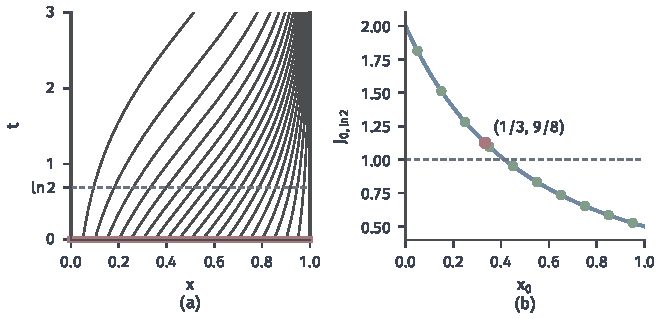
\includegraphics[width=112mm]{figures/06-differential-equations/02-partial-differential-equations/matplotlib/transp-spreading/figure.pdf}
  \caption{Logistic速度场$v=x(1-x)$。(a)从等间距的初始位置（红线）出发的特征线，两端的粗线是不动的边界。(b)$t=\ln2$的体积倍率（蓝），绿点是对流映射做中心差分的结果，红点是例~\ref{ex:transp-logistic-jacobian}的$(1/3,9/8)$，虚线是$J=1$。}
  \label{fig:transp-spreading}
\end{BookInlineFigure}

$\nabla\cdot\bm{v}\equiv0$时，由式~\eqref{eq:transp-liouville-solution}，$J_{s,t}\equiv1$，流映射保持体积。这是第~\ref{sec:transp-flow}节旋转场和鞍点场的共同之处。图~\ref{fig:transp-volume-flows}比较了三种平面流。

旋转场的散度是$\partial_1(-x_2)+\partial_2x_1=0$，鞍点场是$1-1=0$，面积都不变。放大场$\bm{v}=(x_1,x_2)^{\top}$的散度是$2$，$J=\mathrm{e}^{2t}$，$t=\ln2$时面积放大到$4$倍，$0.25$变成了$1$。一般的流要保留这个倍率，不能当作$1$。

\begin{BookInlineFigure}
  \centering
  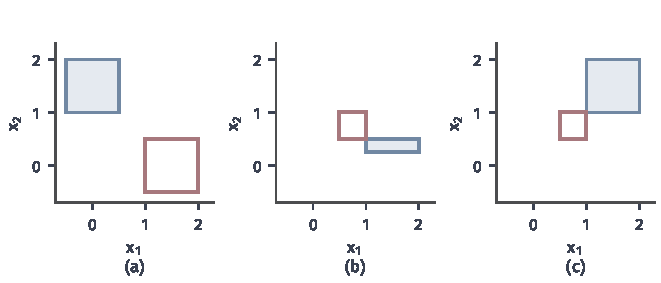
\includegraphics[width=112mm]{figures/06-differential-equations/02-partial-differential-equations/matplotlib/transp-volume-flows/figure.pdf}
  \caption{正方形（红框）被流映射搬运后的像（浅蓝）。(a)旋转场，$t=\pi/2$，面积$1$不变。(b)鞍点场，$t=\ln2$，正方形变成长方形，面积仍为$0.25$。(c)放大场，$t=\ln2$，面积由$0.25$变为$1$。}
  \label{fig:transp-volume-flows}
\end{BookInlineFigure}

\subsection{密度搬运}
\label{sec:transp-density}

有了体积倍率，可以直接算出密度。如图~\ref{fig:transp-pushforward}，一小块区域$\bm{W}$里的质量是$m\approx\rho_0(\bm{x})\lvert\bm{W}\rvert$。流动把它带到$\bm{\varphi}_{0,t}(\bm{W})$，质量不变，体积乘上了$J_{0,t}(\bm{x})$，所以新的密度应当是$\rho_0(\bm{x})/J_{0,t}(\bm{x})$。

\begin{BookInlineFigure}
  \centering
  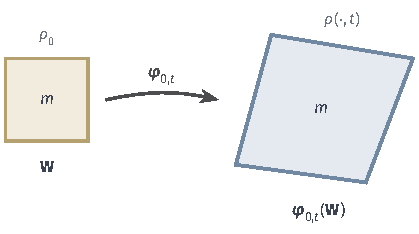
\includegraphics[width=70.9mm]{figures/06-differential-equations/02-partial-differential-equations/tikz/transp-pushforward/figure.pdf}
  \caption{一小块质量被流映射搬运。质量$m$不变，体积变为$J_{0,t}$倍，所以密度除以$J_{0,t}$。}
  \label{fig:transp-pushforward}
\end{BookInlineFigure}

\paragraph{推前测度}
这个想法用测度来说最干净。记初始质量分布为$\mu_0$，$\mathrm{d}\mu_0=\rho_0\,\mathrm{d}\bm{x}$。时刻$t$落在集合$B$中的质量，正好是初始时刻位于$\bm{\varphi}_{t,0}(B)$中的质量，于是
\begin{equation}
  \mu_t(B)=\mu_0\bigl(\bm{\varphi}_{t,0}(B)\bigr),\qquad
  \mu_t=(\bm{\varphi}_{0,t})_{\#}\mu_0.
  \label{eq:transp-pushforward-measure}
\end{equation}
也就是说，$\mu_t$是$\mu_0$在流映射下的推前测度，定义和基本性质见\BookChapterRef{chap:pushforward-measures}{卷四第9章“推前测度”}。

\begin{theorem}[密度搬运公式]
\label{thm:transp-density}
设$\bm{v}$满足条件（V），$\nabla\cdot\bm{v}$关于$\bm{x}$连续可微且偏导数连续，$\rho_0\in C^{1}(\mathbb{R}^{d})$。则方程~\eqref{eq:transp-continuity}（$f=0$）有唯一满足$\rho(\cdot,0)=\rho_0$的$C^{1}$解，它由下式确定：
\begin{equation}
  \rho\bigl(\bm{\varphi}_{0,t}(\bm{x}),t\bigr)\,J_{0,t}(\bm{x})=\rho_0(\bm{x}).
  \label{eq:transp-density}
\end{equation}
进而对任意非负可测函数$h$，有
\begin{equation}
  \int_{\mathbb{R}^{d}}\rho(\bm{y},t)\,h(\bm{y})\,\mathrm{d}\bm{y}
  =\int_{\mathbb{R}^{d}}\rho_0(\bm{x})\,h\bigl(\bm{\varphi}_{0,t}(\bm{x})\bigr)\,\mathrm{d}\bm{x}.
  \label{eq:transp-pushforward}
\end{equation}
若$\rho_0\geq0$，则$\rho\geq0$；取$h=1$，总质量不随时间变化。
\end{theorem}

\begin{proof}
设$\rho$是$C^{1}$解。沿轨迹，由式~\eqref{eq:transp-along}和式~\eqref{eq:transp-liouville}，
\[
  \frac{\mathrm{d}}{\mathrm{d}t}\Bigl[\rho\bigl(\bm{\varphi}_{0,t}(\bm{x}),t\bigr)J_{0,t}(\bm{x})\Bigr]
  =\bigl(\partial_t\rho+\bm{v}\cdot\nabla\rho+\rho\nabla\cdot\bm{v}\bigr)\bigl(\bm{\varphi}_{0,t}(\bm{x}),t\bigr)\,J_{0,t}(\bm{x}).
\]
括号里正是$\partial_t\rho+\nabla\cdot(\rho\bm{v})=0$，所以$\rho J$沿轨迹不变，取$t=0$的值即得式~\eqref{eq:transp-density}，唯一性得证。

反过来，令$R(\bm{x},t)=\rho_0(\bm{x})/J_{0,t}(\bm{x})$。$\nabla\cdot\bm{v}$关于$\bm{x}$是$C^{1}$的，由式~\eqref{eq:transp-liouville-solution}，$J_{0,t}$关于$(\bm{x},t)$是$C^{1}$的且恒正，$R$也是。沿定理~\ref{thm:transp-classical}证明中的映射$\bm{\Psi}$，定义$\rho=R\circ\bm{\Psi}^{-1}$，它是$C^{1}$的，并满足式~\eqref{eq:transp-density}。再用上面的等式把导数读出来，由$J_{0,t}>0$和$\bm{\Psi}$是满射，方程在每一点成立。

式~\eqref{eq:transp-pushforward}由换元$\bm{y}=\bm{\varphi}_{0,t}(\bm{x})$得到。换元产生因子$J_{0,t}$，由式~\eqref{eq:transp-density}，被积函数中$\rho J$恰好等于$\rho_0$：
\[
  \begin{aligned}
  \int\rho(\bm{y},t)h(\bm{y})\,\mathrm{d}\bm{y}
  &=\int\rho\bigl(\bm{\varphi}_{0,t}(\bm{x}),t\bigr)h\bigl(\bm{\varphi}_{0,t}(\bm{x})\bigr)J_{0,t}(\bm{x})\,\mathrm{d}\bm{x}\\
  &=\int\rho_0(\bm{x})h\bigl(\bm{\varphi}_{0,t}(\bm{x})\bigr)\,\mathrm{d}\bm{x}.
  \end{aligned}
\]
非负性由式~\eqref{eq:transp-density}和$J_{0,t}>0$得到。
\end{proof}

式~\eqref{eq:transp-density}是本章的核心：密度倍率$1/J$与体积倍率$J$逐点抵消，乘积沿轨迹不变。取$h$为集合$B$的指示函数，式~\eqref{eq:transp-pushforward}就是式~\eqref{eq:transp-pushforward-measure}。定理还要求$\nabla\cdot\bm{v}$对$\bm{x}$可微，这是为了得到$C^{1}$解；只求弱解时可以去掉，见第~\ref{sec:transp-weak}节。

有源项时，同样的计算给出$\frac{\mathrm{d}}{\mathrm{d}t}[\rho J]=fJ$，沿轨迹积分得到
\begin{equation}
  \rho\bigl(\bm{\varphi}_{0,t}(\bm{x}),t\bigr)\,J_{0,t}(\bm{x})
  =\rho_0(\bm{x})+\int_0^{t}f\bigl(\bm{\varphi}_{0,s}(\bm{x}),s\bigr)\,J_{0,s}(\bm{x})\,\mathrm{d}s.
  \label{eq:transp-density-source}
\end{equation}

\begin{example}[区间上的密度搬运]
\label{ex:transp-logistic-density}
在$(0,1)$上取$v=x(1-x)$，初始密度$\rho_0=1$。由例~\ref{ex:transp-logistic-jacobian}的结果，逆流映射是
\[
  \varphi_{t,0}(y)=\frac{y\mathrm{e}^{-t}}{1-y+y\mathrm{e}^{-t}}.
\]

把$J_{0,t}$用当前位置$y$表示。令$D=1-y+y\mathrm{e}^{-t}$，代入得$1-x+x\mathrm{e}^{t}=1/D$，于是$J_{0,t}=\mathrm{e}^{t}D^{2}$。由式~\eqref{eq:transp-density}，
\[
  \rho(y,t)=\frac{\mathrm{e}^{-t}}{\bigl(1-y+y\mathrm{e}^{-t}\bigr)^{2}}.
\]

取$t=\ln2$，$y=1/2$。出发位置是$x=\varphi_{\ln2,0}(1/2)=1/3$，倍率是$9/8$，所以
\[
  \rho(1/2,\ln2)=\frac{8}{9}.
\]
代入上面的公式核对：$D=3/4$，$\rho=\tfrac12\cdot\tfrac{16}{9}=\tfrac89$。

再验证总质量。$t=\ln2$时$\rho(y,\ln 2)=\tfrac12(1-y/2)^{-2}$，
\[
  \int_0^{1}\frac12\Bigl(1-\frac{y}{2}\Bigr)^{-2}\mathrm{d}y=\Bigl[\frac{1}{1-y/2}\Bigr]_0^{1}=2-1=1.
\]
\end{example}

图~\ref{fig:transp-logistic-density}(a)是这个密度在不同时刻的形状。均匀的初始分布逐渐向右端集中，绿色直方图是$40000$个按初始分布抽取的粒子在$t=\ln4$的位置，与公式吻合。

(b)从另一个角度看。质量$\int_0^{y}\rho\,\mathrm{d}x$等于初始时位于$(0,\varphi_{t,0}(y))$中的质量，而$\rho_0=1$，所以累积质量恰好是逆流映射本身。$t=\ln2$时，左半区间的质量是$\varphi_{\ln2,0}(1/2)=1/3$。

\begin{BookInlineFigure}
  \centering
  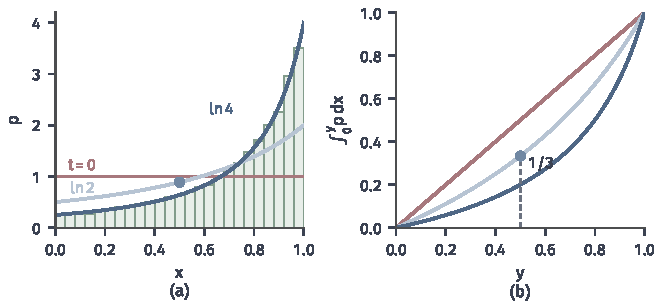
\includegraphics[width=112mm]{figures/06-differential-equations/02-partial-differential-equations/matplotlib/transp-logistic-density/figure.pdf}
  \caption{$(0,1)$上$v=x(1-x)$对均匀密度的搬运。(a)密度$\rho$：$t=0$（红）、$t=\ln2$与$t=\ln4$（蓝色由浅到深），绿色直方图是$40000$个粒子（固定种子）在$t=\ln4$的分布，蓝点是$(1/2,8/9)$。(b)累积质量，蓝点表示$t=\ln2$时左半区间的质量为$1/3$。}
  \label{fig:transp-logistic-density}
\end{BookInlineFigure}

平面上的情形相同。图~\ref{fig:transp-density-2d}把一个Gaussian形的密度分别交给三种流，运行时间都是$t=1$，初始峰值是$1$。放大场$\bm{v}=\bm{x}/2$的散度是$1$，峰值降到$\mathrm{e}^{-1}\approx0.37$；鞍点场$\bm{v}=(x_1/2,-x_2/2)^{\top}$的散度是$0$，形状变了，峰值不变；收缩场$\bm{v}=-\bm{x}/2$的散度是$-1$，峰值升到$\mathrm{e}\approx2.72$。

\begin{BookInlineFigure}
  \centering
  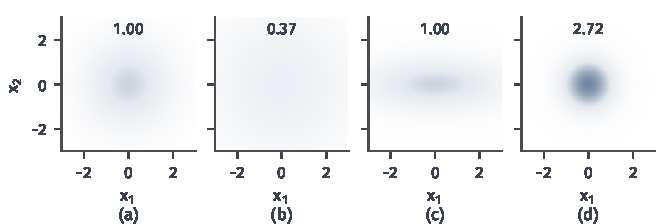
\includegraphics[width=112mm]{figures/06-differential-equations/02-partial-differential-equations/matplotlib/transp-density-2d/figure.pdf}
  \caption{同一Gaussian形密度的搬运，蓝色越深密度越大，图中数字是峰值。(a)初值。(b)放大场，$t=1$。(c)无散度的鞍点场，$t=1$。(d)收缩场，$t=1$。四幅图共用一个色阶。}
  \label{fig:transp-density-2d}
\end{BookInlineFigure}

概率密度是这里的特例：$\rho_0\geq0$且总质量为$1$。定理~\ref{thm:transp-density}说明这两条性质都被流保持，所以时刻$t$的$\rho$仍是概率密度，$\bm{\varphi}_{0,t}$就是随机变量的变换。除此之外，归一化没有增加任何东西，这里讨论的是一般的守恒密度。

表~\ref{tab:transp-value-density}把两种量并排列出。

\begin{BookInlineTable}
  \centering
  \caption{沿轨迹的场值与密度的比较。设$\bm{v}$满足条件（V），无源项。}
  \label{tab:transp-value-density}
  \begin{tabular}{p{16mm}p{42mm}p{42mm}}
    \toprule
    & 场值$u$ & 密度$\rho$ \\
    \midrule
    方程 & $\partial_tu+\bm{v}\cdot\nabla u=0$ & $\partial_t\rho+\nabla\cdot(\rho\bm{v})=0$ \\
    沿轨迹 & $u$不变 & $\rho J$不变 \\
    解 & $u_0\circ\bm{\varphi}_{t,0}$ & $(\rho_0/J_{0,t})\circ\bm{\varphi}_{t,0}$ \\
    不变量 & 最大值、最小值 & 总质量 \\
    例$v=x$，$t=\ln2$ & 高度不变，面积翻倍 & 高度减半，面积不变 \\
    \bottomrule
  \end{tabular}
\end{BookInlineTable}

\subsection{边界通量}
\label{sec:transp-boundary-flux}

全空间上质量不变，是因为没有地方可去。在有界区域里，粒子可能离开，也可能有新的粒子进入，总质量的变化完全由边界决定。

\paragraph{流入、流出与无通量}
在式~\eqref{eq:transp-balance}中取$W=\Omega$，把边界分成三部分：
\begin{equation}
  \Gamma_{-}=\{\bm{v}\cdot\bm{n}<0\},\qquad
  \Gamma_{+}=\{\bm{v}\cdot\bm{n}>0\},\qquad
  \Gamma_{0}=\{\bm{v}\cdot\bm{n}=0\}.
  \label{eq:transp-boundary-parts}
\end{equation}
图~\ref{fig:transp-boundary-parts}是匀速水平流过圆盘时的三部分。$\Gamma_{-}$上给定密度$\rho=g$（质量随粒子进入），$\Gamma_{+}$上的值由内部决定，$\Gamma_{0}$上没有流量。

总质量$M(t)=\int_\Omega\rho\,\mathrm{d}\bm{x}$的变化率是
\begin{equation}
  M'(t)=\int_{\Gamma_{-}}g\,\lvert\bm{v}\cdot\bm{n}\rvert\,\mathrm{d}S
  -\int_{\Gamma_{+}}\rho\,\bm{v}\cdot\bm{n}\,\mathrm{d}S
  +\int_\Omega f\,\mathrm{d}\bm{x}.
  \label{eq:transp-mass-rate}
\end{equation}

\begin{BookInlineFigure}
  \centering
  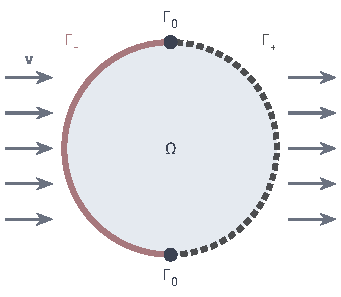
\includegraphics[width=57.8mm]{figures/06-differential-equations/02-partial-differential-equations/tikz/transp-boundary-parts/figure.pdf}
  \caption{速度场$\bm{v}=(1,0)^{\top}$（灰色箭头）下，圆盘的边界分成三部分：红色实线是入流边界$\Gamma_{-}$，深灰虚线是出流边界$\Gamma_{+}$，上下两点是$\bm{v}\cdot\bm{n}=0$的$\Gamma_{0}$。}
  \label{fig:transp-boundary-parts}
\end{BookInlineFigure}

下面在$(0,1)$上取$\rho_0=1$，看三个例子，$M(0)=1$。

第一，$v=1$，$g=0$。这时$\rho(x,t)=1$（$x>t$）、$\rho=0$（$x<t$）。质量以单位速率从右端流出，所以
\[
  M(t)=\max\{1-t,\ 0\}.
\]
式~\eqref{eq:transp-mass-rate}的流出项在$t<1$时等于$\rho(1,t)\cdot1=1$，符合$M'=-1$。

第二，$v=x-1/2$，两端都是出流。解是$\rho=\mathrm{e}^{-t}$，代入验证：
\[
  \partial_t\rho=-\mathrm{e}^{-t},\qquad \partial_x\bigl(\rho\,(x-\tfrac12)\bigr)=\mathrm{e}^{-t}.
\]
两端的流出量都是$\tfrac12\mathrm{e}^{-t}$，合起来恰好是$M'=-\mathrm{e}^{-t}$，因此
\[
  M(t)=\mathrm{e}^{-t}.
\]

第三，$v=x(1-x)$，两端$v=0$，边界是无通量的。例~\ref{ex:transp-logistic-density}中质量向右端堆积，但始终没有离开区间，
\[
  M(t)=1.
\]

这三种情形对应图~\ref{fig:transp-mass-balance}。把第一例换成$g=2$，则$t<1$时左端流入$2$、右端流出$1$，$M=1+t$；$t\geq1$时整个区间密度为$2$，进出相等，$M=2$。

\begin{BookInlineFigure}
  \centering
  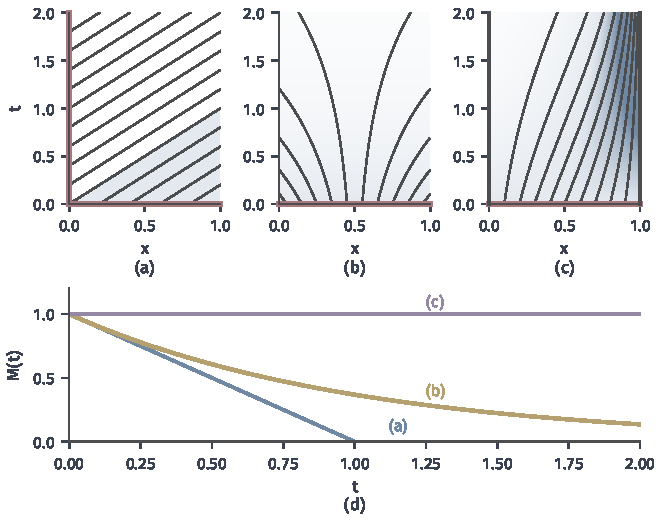
\includegraphics[width=112mm]{figures/06-differential-equations/02-partial-differential-equations/matplotlib/transp-mass-balance/figure.pdf}
  \caption{$(0,1)$上的质量平衡，$\rho_0=1$。上排是特征线（深灰）和密度（蓝色越深越大）：(a)$v=1$，入流数据为$0$；(b)$v=x-1/2$，两端出流；(c)$v=x(1-x)$，两端无通量（粗线）。红线是给数据的边界。(d)三种情形的总质量$M(t)$。}
  \label{fig:transp-mass-balance}
\end{BookInlineFigure}

质量守恒是一个有条件的结论。只有当右端全部为零时，$M$才不变，典型条件是$\Omega$封闭，即$\partial\Omega$上$\bm{v}\cdot\bm{n}=0$，并且没有源项。此时轨迹不会穿过边界，流映射把$\Omega$映到自身，定理~\ref{thm:transp-density}的论证可以在$\Omega$上进行，例~\ref{ex:transp-logistic-density}就是这样。否则，全空间上的守恒结论不能照搬到有界区域。

\section{弱形式}
\label{sec:transp-weak}

三角形初值有折角，台阶初值有跳跃，这些初值都没有经典解的资格，可是特征线公式照样给出了合理的函数。怎样说它们“满足方程”？第~\ref{chap:pde-problems}章的办法是把导数转移到测试函数上。输运方程和连续性方程的导数位置不同，转移之后的结果也不同，所以要分别处理。

下面取$\Omega=\mathbb{R}^{d}$，设$\bm{v}$满足条件（V），测试函数$\psi\in C^{1}_{c}(\mathbb{R}^{d}\times[0,T))$，它在$t=T$附近为零，在$t=0$可以不为零。

\paragraph{两个弱形式}
设$u$是输运方程的经典解。乘以$\psi$，在$\mathbb{R}^{d}\times(0,T)$上积分。时间项对$t$分部积分，产生初值的边界项；空间项写成$\psi\bm{v}\cdot\nabla u$，对$\bm{x}$分部积分，导数要落到$\psi\bm{v}$上。

得到的关系里不再有$u$的导数，只有$\psi\bm{v}$的散度
\[
  \nabla\cdot(\psi\bm{v})=\bm{v}\cdot\nabla\psi+\psi\,\nabla\cdot\bm{v}.
\]

连续性方程的空间项本来就是散度，分部积分后导数只落在$\psi$上，$\bm{v}$不被求导。

\begin{definition}[输运方程与连续性方程的弱解]
\label{def:transp-weak}
设$u_0,\rho_0\in L^{1}_{\mathrm{loc}}(\mathbb{R}^{d})$，$f\in L^{1}_{\mathrm{loc}}(\mathbb{R}^{d}\times[0,T))$。称$u\in L^{1}_{\mathrm{loc}}(\mathbb{R}^{d}\times[0,T))$是输运方程的弱解，若对所有测试函数$\psi$，有
\begin{equation}
  \int_0^{T}\!\!\int u\bigl(\partial_t\psi+\nabla\cdot(\psi\bm{v})\bigr)\,\mathrm{d}\bm{x}\,\mathrm{d}t
  +\int u_0\,\psi(\cdot,0)\,\mathrm{d}\bm{x}
  +\int_0^{T}\!\!\int f\psi\,\mathrm{d}\bm{x}\,\mathrm{d}t=0.
  \label{eq:transp-weak-transport}
\end{equation}
称$\rho\in L^{1}_{\mathrm{loc}}(\mathbb{R}^{d}\times[0,T))$是连续性方程的弱解，若对所有测试函数$\psi$，有
\begin{equation}
  \int_0^{T}\!\!\int\rho\bigl(\partial_t\psi+\bm{v}\cdot\nabla\psi\bigr)\,\mathrm{d}\bm{x}\,\mathrm{d}t
  +\int\rho_0\,\psi(\cdot,0)\,\mathrm{d}\bm{x}
  +\int_0^{T}\!\!\int f\psi\,\mathrm{d}\bm{x}\,\mathrm{d}t=0.
  \label{eq:transp-weak-continuity}
\end{equation}
\end{definition}

两式都不含未知函数的导数，所以间断函数也可以代入。对比可以发现，式~\eqref{eq:transp-weak-transport}中出现了$\nabla\cdot\bm{v}$，要求速度场的散度是函数；式~\eqref{eq:transp-weak-continuity}只需要$\rho\bm{v}$局部可积，对$\bm{v}$的要求弱得多。

分部积分的步骤可逆，所以当$u$或$\rho$是$C^{1}$函数时，弱解就是经典解。下面用一个例子看看弱形式如何辨别间断的传播速度。

\begin{example}[台阶的传播速度]
\label{ex:transp-step}
取一维$v=1$，$f=0$，台阶初值$u_0=1$（$x<0$）、$u_0=0$（$x>0$）。考虑以速度$s>0$移动的台阶$u_s=1$（$x<st$）、$u_s=0$（$x>st$）。

把$u_s$代入式~\eqref{eq:transp-weak-transport}，记左端为$R(s)$，并令$I=\int_0^{T}\psi(st,t)\,\mathrm{d}t$。先算空间项，由微积分基本定理，
\[
  \int_0^{T}\!\!\int_{-\infty}^{st}\partial_x\psi\,\mathrm{d}x\,\mathrm{d}t=I.
\]

再算时间项。积分上限随时间移动，由含参积分的求导法则，
\[
  \frac{\mathrm{d}}{\mathrm{d}t}\int_{-\infty}^{st}\psi\,\mathrm{d}x=\int_{-\infty}^{st}\partial_t\psi\,\mathrm{d}x+s\psi(st,t).
\]
对$t$从$0$到$T$积分，
\[
  \int_0^{T}\!\!\int_{-\infty}^{st}\partial_t\psi\,\mathrm{d}x\,\mathrm{d}t
  =-\int_{-\infty}^{0}\psi(x,0)\,\mathrm{d}x-sI.
\]

两项相加，再加上初值项$\int_{-\infty}^{0}\psi(x,0)\,\mathrm{d}x$，初值积分抵消，
\[
  R(s)=(1-s)\,I.
\]
只要存在使$I\neq0$的测试函数，$R(s)=0$就等价于$s=1$。所以台阶的弱解只能以特征速度$1$移动。
\end{example}

图~\ref{fig:transp-weak-step}(a)的紫色等值线是一个测试函数，它跨在间断线的两侧。(b)用光滑的初值逼近台阶，光滑解$u_0^{\varepsilon}(x-t)$在$\varepsilon\to0$时收敛到台阶解，这也说明台阶解是光滑解的极限。(c)对一个具体的$\psi$计算了$R(s)$，绿点是数值积分的结果，只有$s=1$时为零。

\begin{BookInlineFigure}
  \centering
  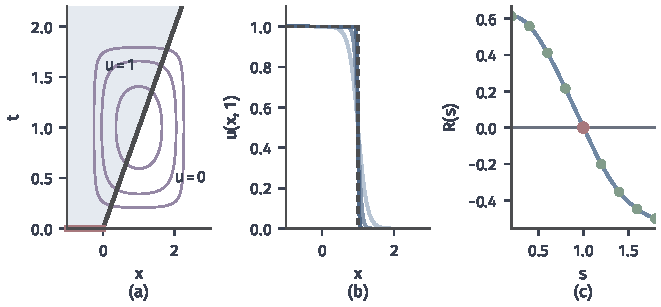
\includegraphics[width=112mm]{figures/06-differential-equations/02-partial-differential-equations/matplotlib/transp-weak-step/figure.pdf}
  \caption{台阶解的弱形式，$v=1$。(a)左侧浅蓝区域$u=1$，深灰粗线是间断线$x=t$，紫色曲线是测试函数$\psi$的等值线，红线是初值$1$的部分。(b)光滑化初值的解在$t=1$的剖面（蓝色由浅到深，过渡带越来越窄），虚线是台阶解。(c)$R(s)=(1-s)\int\psi(st,t)\,\mathrm{d}t$（蓝）与数值积分（绿），红点是$s=1$。}
  \label{fig:transp-weak-step}
\end{BookInlineFigure}

\paragraph{流构造就是弱解}
一般的情形下，第~\ref{sec:transp-flow}节的公式对粗糙的数据仍给出弱解，并且在$\bm{v}$足够正则时它是唯一的。

\begin{theorem}[流构造给出弱解]
\label{thm:transp-weak}
设$\bm{v}$满足条件（V）。
\begin{enumerate}
  \item 对$\rho_0\in L^{1}_{\mathrm{loc}}(\mathbb{R}^{d})$，函数
  \begin{equation}
    \rho(\bm{y},t)=\rho_0\bigl(\bm{\varphi}_{t,0}(\bm{y})\bigr)\,J_{t,0}(\bm{y})
    \label{eq:transp-weak-density}
  \end{equation}
  是连续性方程（$f=0$）的弱解，且是$L^{1}_{\mathrm{loc}}$中唯一的弱解。
  \item 对$u_0\in L^{1}_{\mathrm{loc}}(\mathbb{R}^{d})$，$u=u_0\circ\bm{\varphi}_{t,0}$是输运方程（$f=0$）的弱解。若$\nabla\cdot\bm{v}$还关于$\bm{x}$连续可微，这个弱解是$L^{1}_{\mathrm{loc}}$中唯一的。
\end{enumerate}
\end{theorem}

\begin{proof}
先证$\rho$是弱解。固定$\bm{x}$，由式~\eqref{eq:transp-flow}，沿轨迹有
\[
  \frac{\mathrm{d}}{\mathrm{d}t}\psi\bigl(\bm{\varphi}_{0,t}(\bm{x}),t\bigr)
  =\bigl(\partial_t\psi+\bm{v}\cdot\nabla\psi\bigr)\bigl(\bm{\varphi}_{0,t}(\bm{x}),t\bigr).
\]

在$[0,T]$上积分。$\psi$在$t=T$附近为零，于是
\[
  -\psi(\bm{x},0)=\int_0^{T}\bigl(\partial_t\psi+\bm{v}\cdot\nabla\psi\bigr)\bigl(\bm{\varphi}_{0,t}(\bm{x}),t\bigr)\,\mathrm{d}t.
\]

两边乘以$\rho_0(\bm{x})$，对$\bm{x}$积分并交换积分次序。式~\eqref{eq:transp-weak-density}的$\rho$满足式~\eqref{eq:transp-density}，换元$\bm{y}=\bm{\varphi}_{0,t}(\bm{x})$后，右端正是$\int_0^{T}\!\int\rho(\partial_t\psi+\bm{v}\cdot\nabla\psi)\,\mathrm{d}\bm{y}\,\mathrm{d}t$，这就是式~\eqref{eq:transp-weak-continuity}。

再证$u$是弱解。沿轨迹求导时多带一个因子$J_{0,t}$，由式~\eqref{eq:transp-liouville}，
\[
  \frac{\mathrm{d}}{\mathrm{d}t}\Bigl[\psi\bigl(\bm{\varphi}_{0,t}(\bm{x}),t\bigr)J_{0,t}(\bm{x})\Bigr]
  =\bigl(\partial_t\psi+\nabla\cdot(\psi\bm{v})\bigr)\bigl(\bm{\varphi}_{0,t}(\bm{x}),t\bigr)\,J_{0,t}(\bm{x}).
\]
对$t$积分，初值是$\psi(\bm{x},0)$。乘以$u_0(\bm{x})$，对$\bm{x}$积分，再把$\mathrm{d}\bm{x}$上的$J_{0,t}$用换元吸收，得到式~\eqref{eq:transp-weak-transport}。

接着证连续性方程的唯一性。设$\rho$是$\rho_0=0$的弱解，任取$h\in C^{1}_{c}(\mathbb{R}^{d}\times(0,T))$。定义
\[
  \psi(\bm{x},t)=-\int_t^{T}h\bigl(\bm{\varphi}_{t,r}(\bm{x}),r\bigr)\,\mathrm{d}r.
\]

由式~\eqref{eq:transp-flow-rules}，$\bm{\varphi}_{t,r}$是$\bm{\varphi}_{0,r}$与$\bm{\varphi}_{t,0}$的复合，关于$(\bm{x},t)$是$C^{1}$的，所以$\psi\in C^{1}$。$\psi$在$t=T$附近为零，$h$的支集紧，流映射连续，所以$\psi$的支集也紧，它是合法的测试函数。

任取一条轨迹$\bm{Y}(t)$，由定义，
\[
  \psi\bigl(\bm{Y}(t),t\bigr)=-\int_t^{T}h\bigl(\bm{Y}(r),r\bigr)\,\mathrm{d}r.
\]
对$t$求导，得到
\[
  \partial_t\psi+\bm{v}\cdot\nabla\psi=h.
\]
代入式~\eqref{eq:transp-weak-continuity}，得到
\[
  \int_0^{T}\!\!\int\rho h\,\mathrm{d}\bm{x}\,\mathrm{d}t=0.
\]
这对所有$h$成立，所以$\rho=0$几乎处处成立。

最后证输运方程的唯一性。令$c=\nabla\cdot\bm{v}$，取同样的$h$，定义
\[
  \psi(\bm{x},t)=-\int_t^{T}h\bigl(\bm{\varphi}_{t,r}(\bm{x}),r\bigr)\exp\Bigl(\int_t^{r}c\bigl(\bm{\varphi}_{t,\tau}(\bm{x}),\tau\bigr)\,\mathrm{d}\tau\Bigr)\mathrm{d}r.
\]

$c$关于$\bm{x}$是$C^{1}$的，所以$\psi\in C^{1}$，这就是额外假设的作用。沿轨迹用积分因子，得到$\partial_t\psi+\bm{v}\cdot\nabla\psi+c\psi=h$，即$\partial_t\psi+\nabla\cdot(\psi\bm{v})=h$。代入式~\eqref{eq:transp-weak-transport}，同样推出$u=0$。
\end{proof}

有源项时，解按式~\eqref{eq:transp-flow-solution}和式~\eqref{eq:transp-density-source}叠加，证明的计算相同，唯一性的结论也不变。

这个证明还揭示了两个方程之间的对偶关系。若$u$满足无源输运方程、$\rho$满足无源连续性方程，且二者足够光滑、衰减足够快，那么直接求导，用分部积分，可得
\[
  \frac{\mathrm{d}}{\mathrm{d}t}\int\rho u\,\mathrm{d}\bm{x}
  =\int\bigl(u\,\partial_t\rho+\rho\,\partial_tu\bigr)\,\mathrm{d}\bm{x}
  =\int\bigl(-u\nabla\cdot(\rho\bm{v})-\rho\bm{v}\cdot\nabla u\bigr)\,\mathrm{d}\bm{x}=0.
\]
也就是说，质量加权的标签总量不随时间变化。$h$与$\psi$的构造正是在利用这一点。

\paragraph{测度形式}
由于式~\eqref{eq:transp-weak-continuity}中不含$\bm{v}$的导数，也可以让$\rho_0$是测度。把积分$\int\rho_0\psi\,\mathrm{d}\bm{x}$换成$\int\psi\,\mathrm{d}\mu_0$，就可以描述集中在一点的质量。

取$\mu_0=\delta_{\bm{x}_0}$，式~\eqref{eq:transp-pushforward-measure}给出$\mu_t=\delta_{\bm{\varphi}_{0,t}(\bm{x}_0)}$，这个Dirac质量跟着粒子走。这是第~\ref{sec:transp-continuity}节密度搬运的极端情形，此时密度不再是函数，但质量守恒和推前关系仍然成立。

\paragraph{粗糙速度场}
以上结论都建立在条件（V）上。把$\bm{v}$换成粗糙的场，弱形式的写法没有变化，定理~\ref{thm:transp-weak}的结论却可能失效。

看图~\ref{fig:transp-rough-velocity}中的两个间断速度场。(a)$v=-\mathrm{sgn}(x)$：粒子从两侧撞向原点。$\rho_0=1$（$\lvert x\rvert<1$）时，$t<1$时的质量分布是
\begin{equation}
  \mu_t=\mathbf{1}_{\lvert x\rvert<1-t}\,\mathrm{d}x+2t\,\delta_0.
  \label{eq:transp-collision}
\end{equation}
质量在原点集中成Dirac，不再是函数。$\delta_0$处还需要规定$v$的取值，式~\eqref{eq:transp-collision}用的是$v(0)=0$，这个零测集上的取值现在影响结论。

(b)$v=\mathrm{sgn}(x)$：粒子从原点向两侧分开，$\lvert x\rvert<t$形成一块没有粒子来过的区域，浅红色部分。对输运方程来说，这里的值没有被初值决定。

对连续性方程，唯一性也会失败。看(c)：取$v=\mathrm{sgn}(x)$，初值$\rho_0=0$，定义
\begin{equation}
  \rho(x,t)=
  \begin{cases}
    t-x, & 0<x<t,\\
    -(t+x), & -t<x<0,\\
    0, & \text{其他}.
  \end{cases}
  \label{eq:transp-nonunique-density}
\end{equation}

\begin{BookInlineFigure}
  \centering
  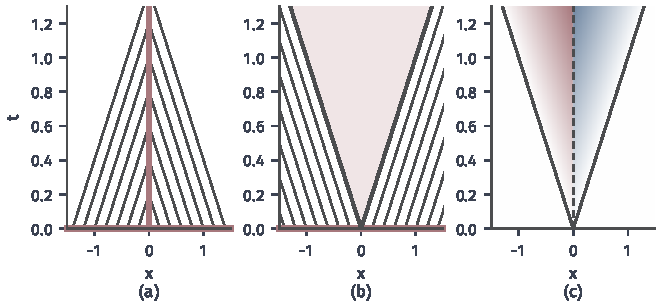
\includegraphics[width=112mm]{figures/06-differential-equations/02-partial-differential-equations/matplotlib/transp-rough-velocity/figure.pdf}
  \caption{间断速度场的三种问题，红线在(a)(b)中是初始线。(a)$v=-\mathrm{sgn}(x)$，特征线（深灰）撞向原点，红色粗线处积累质量。(b)$v=\mathrm{sgn}(x)$，浅红区域没有特征线到达。(c)$v=\mathrm{sgn}(x)$、$\rho_0=0$时的非零弱解~\eqref{eq:transp-nonunique-density}，红—白—蓝色阶的中点为$0$。}
  \label{fig:transp-rough-velocity}
\end{BookInlineFigure}

验证如下。在$x>0$的一侧，$v=1$，$\rho=t-x$满足$\partial_t\rho+\partial_x\rho=1-1=0$；$x<0$一侧，$v=-1$，$\rho=-(t+x)$满足$\partial_t\rho-\partial_x\rho=-1+1=0$。在分界线$x=0$上，右侧流量$\rho v=t\cdot1=t$，左侧流量$(-t)\cdot(-1)=t$，两侧相等，所以弱形式成立。

沿$x=\pm t$，$\rho$连续，没有问题。于是初值为零的问题有非零弱解，弱解在这里不唯一。式~\eqref{eq:transp-nonunique-density}的$\rho$有正有负，它在$x=0$两侧同时“产生”正、负质量。

这些例子都说明，弱形式并不会自动带来好的理论。超出Lipschitz范围的速度场需要专门的工具，结论依赖于$\nabla\bm{v}$的Sobolev型正则性和散度的有界性，这已超出本章的范围。本章的结论不能自动推广到任意粗糙的速度场。

\paragraph{有界区域上的弱形式}
有界区域的连续性方程也有相应的写法。要把$\Gamma_{-}$上的入流数据$g$放进去，测试函数应在$\Gamma_{+}$上为零。乘以$\psi$后分部积分，得到
\begin{equation}
  \int_0^{T}\!\!\int_{\Omega}\rho\bigl(\partial_t\psi+\bm{v}\cdot\nabla\psi\bigr)\,\mathrm{d}\bm{x}\,\mathrm{d}t
  +\int_{\Omega}\rho_0\psi(\cdot,0)\,\mathrm{d}\bm{x}
  +\int_0^{T}\!\!\int_{\Gamma_{-}}g\,\lvert\bm{v}\cdot\bm{n}\rvert\,\psi\,\mathrm{d}S\,\mathrm{d}t=0.
  \label{eq:transp-weak-boundary}
\end{equation}
边界项与式~\eqref{eq:transp-mass-rate}的入流项相对应，$\Gamma_{+}$上$\psi=0$让未知的出流值不进入方程。

\section{数据稳定性}
\label{sec:transp-stability}

测量得到的初值、源项和速度场总有误差。这些误差会被放大多少？答案与所用的范数有关，也与误差出现在哪个量上有关。

\paragraph{数据误差的$L^p$估计}
输运方程对$u$是线性的，同一速度场下，两个解的差$e$满足同一方程，其初值和源项分别是初值之差$e_0$与源项之差$g_e$。所以只需估计式~\eqref{eq:transp-flow-solution}给出的$e$。

要点是：逆流映射$\bm{\varphi}_{t,s}$的复合不改变函数的最大值，但会改变$L^{p}$范数，因为积分时要换元。这时$J_{s,t}$进入估计。

\begin{theorem}[数据误差的$L^{p}$估计]
\label{thm:transp-lp}
设$\bm{v}$满足条件（V），存在常数$\kappa\geq0$使$\nabla\cdot\bm{v}\leq\kappa$。设$1\leq p<\infty$，$e_0\in L^{p}(\mathbb{R}^{d})$，$g_e\in L^{1}(0,T;L^{p}(\mathbb{R}^{d}))$，$e$由式~\eqref{eq:transp-flow-solution}给出。则对$t\in[0,T]$，
\begin{equation}
  \lVert e(\cdot,t)\rVert_{p}\leq\mathrm{e}^{\kappa t/p}\lVert e_0\rVert_{p}
  +\int_0^{t}\mathrm{e}^{\kappa(t-s)/p}\lVert g_e(\cdot,s)\rVert_{p}\,\mathrm{d}s.
  \label{eq:transp-lp-estimate}
\end{equation}
当$e_0\in L^{\infty}$，$g_e\in L^{1}(0,T;L^{\infty})$时，把上式中的$\mathrm{e}^{\kappa\cdot/p}$换成$1$，无需假设散度有上界，结论对$p=\infty$成立。
\end{theorem}

\begin{proof}
先看单个函数的复合。设$w\in L^{p}$，换元$\bm{y}=\bm{\varphi}_{t,s}(\bm{x})$，即$\bm{x}=\bm{\varphi}_{s,t}(\bm{y})$，体积元多出因子$J_{s,t}(\bm{y})$，得到
\[
  \int\bigl\lvert w\bigl(\bm{\varphi}_{t,s}(\bm{x})\bigr)\bigr\rvert^{p}\,\mathrm{d}\bm{x}
  =\int\lvert w(\bm{y})\rvert^{p}J_{s,t}(\bm{y})\,\mathrm{d}\bm{y}.
\]

由式~\eqref{eq:transp-liouville-solution}和$\nabla\cdot\bm{v}\leq\kappa$，$J_{s,t}\leq\mathrm{e}^{\kappa(t-s)}$。开$p$次方，
\[
  \lVert w\circ\bm{\varphi}_{t,s}\rVert_{p}\leq\mathrm{e}^{\kappa(t-s)/p}\lVert w\rVert_{p}.
\]

把这个估计用于式~\eqref{eq:transp-flow-solution}的第一项，以及第二项中被积函数的$L^p$范数，再用Minkowski积分不等式把范数移入积分号，就得到式~\eqref{eq:transp-lp-estimate}。对$p=\infty$，复合映射双射，本性上确界不变，同样的步骤给出结论，$J$不再出现。
\end{proof}

式~\eqref{eq:transp-lp-estimate}表明，放大来自局部的体积膨胀：$p$越大，因子$\mathrm{e}^{\kappa t/p}$越接近$1$，$p=\infty$时不放大。

对例~\ref{ex:transp-stretch}的$v=x$，有$\kappa=1$，$J_{0,t}=\mathrm{e}^{t}$是常数。此时$e(x,t)=e_0(x\mathrm{e}^{-t})$，换元得到精确的等式：
\begin{equation}
  \lVert e(\cdot,t)\rVert_{p}=\mathrm{e}^{t/p}\lVert e_0\rVert_{p},
  \label{eq:transp-lp-example}
\end{equation}
所以式~\eqref{eq:transp-lp-estimate}中的因子不能再改进。

密度的情形相反。$\rho$按式~\eqref{eq:transp-density}搬运时，换元给出
\begin{equation}
  \lVert\rho(\cdot,t)\rVert_{p}^{p}=\int\lvert\rho_0(\bm{x})\rvert^{p}\,J_{0,t}(\bm{x})^{1-p}\,\mathrm{d}\bm{x}.
  \label{eq:transp-density-lp}
\end{equation}
$p=1$时$J$的幂次为零，$L^{1}$范数不变，这是质量守恒的范数形式。$p>1$时，密度的误差在压缩处被放大，在膨胀处被缩小，放大倍数由$\inf J_{0,t}$控制。

图~\ref{fig:transp-stability-lp}比较了$v=x$下三角形误差的范数，(a)是$u$的误差，(b)是$\rho$的误差。$u$的$L^{1}$误差增长最快，$L^{\infty}$不变；$\rho$恰好反过来，$L^{1}$不变，$L^{\infty}$衰减最快。线是精确的指数公式，绿点是数值积分。

\begin{BookInlineFigure}
  \centering
  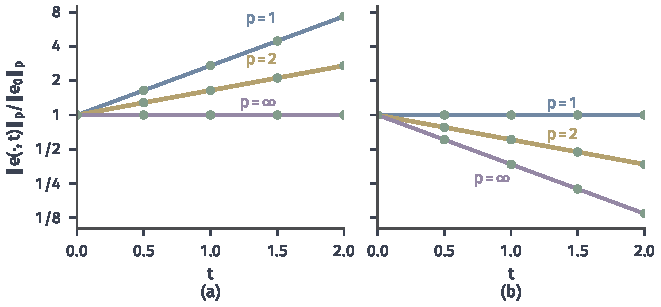
\includegraphics[width=112mm]{figures/06-differential-equations/02-partial-differential-equations/matplotlib/transp-stability-lp/figure.pdf}
  \caption{速度场$v=x$下误差范数的变化（纵轴为对数），$p=1,2,\infty$依次为蓝、黄、紫，绿点是用数值积分算出的范数比。(a)场值误差，满足式~\eqref{eq:transp-lp-example}。(b)密度误差，因子为$\mathrm{e}^{-(1-1/p)t}$。}
  \label{fig:transp-stability-lp}
\end{BookInlineFigure}

\paragraph{比较两个速度场}
现在让速度场本身有误差，初值和源项相同。上面的线性结构用不上了，因为$u^{a}$与$u^{b}$沿不同的轨迹搬运。此时的思路是比较两组特征线，再用数据的空间Lipschitz常数把轨迹差转换为场值差。

\begin{theorem}[速度场误差的$L^{\infty}$估计]
\label{thm:transp-velocity}
设$\bm{v}^{a},\bm{v}^{b}$满足条件（V），其中$\bm{v}^{a}$的常数为$L$，并存在可积函数$\delta$，使
\begin{equation}
  \lVert\bm{v}^{a}(\bm{x},t)-\bm{v}^{b}(\bm{x},t)\rVert_2\leq\delta(t).
  \label{eq:transp-velocity-gap}
\end{equation}
设$u_0$是$L_0$-Lipschitz函数，$f(\cdot,s)$是$L_f$-Lipschitz函数（常数不依赖$s$）。令$u^{a},u^{b}$分别是由式~\eqref{eq:transp-flow-solution}给出的解，定义
\begin{equation}
  E(t,s)=\int_s^{t}\mathrm{e}^{L(r-s)}\delta(r)\,\mathrm{d}r.
  \label{eq:transp-velocity-integral}
\end{equation}
则
\begin{equation}
  \lVert u^{a}(\cdot,t)-u^{b}(\cdot,t)\rVert_{\infty}
  \leq L_0\,E(t,0)+L_f\int_0^{t}E(t,s)\,\mathrm{d}s.
  \label{eq:transp-velocity-estimate}
\end{equation}
\end{theorem}

\begin{proof}
固定$\bm{x}$和$t$，令$\bm{x}^{a}(r)=\bm{\varphi}^{a}_{t,r}(\bm{x})$，$\bm{x}^{b}$同理，$z(r)=\lVert\bm{x}^{a}(r)-\bm{x}^{b}(r)\rVert_2$。两条曲线在$r=t$处重合，从$r$到$t$积分两者的差，
\[
  \bm{x}^{a}(r)-\bm{x}^{b}(r)
  =-\int_r^{t}\bigl(\bm{v}^{a}(\bm{x}^{a},\tau)-\bm{v}^{b}(\bm{x}^{b},\tau)\bigr)\,\mathrm{d}\tau.
\]

在被积函数中加减$\bm{v}^{a}(\bm{x}^{b},\tau)$，第一组差用$L$，第二组差用$\delta$，于是
\[
  z(r)\leq Z(r):=\int_r^{t}\bigl(Lz(\tau)+\delta(\tau)\bigr)\,\mathrm{d}\tau.
\]

由$-Z'(r)=Lz+\delta\leq LZ+\delta$，乘以积分因子，
\[
  \frac{\mathrm{d}}{\mathrm{d}r}\Bigl[\mathrm{e}^{L(r-s)}Z(r)\Bigr]
  =\mathrm{e}^{L(r-s)}\bigl(LZ(r)+Z'(r)\bigr)\geq-\mathrm{e}^{L(r-s)}\delta(r).
\]

从$s$到$t$积分，并用$Z(t)=0$，
\[
  z(s)\leq Z(s)\leq\int_s^{t}\mathrm{e}^{L(r-s)}\delta(r)\,\mathrm{d}r=E(t,s).
\]

这是反向的Gronwall估计，相当于第~\ref{chap:ode-sensitivity}章的结论在时间翻转下的形式。把它代入式~\eqref{eq:transp-flow-solution}，两项分别用$u_0$和$f(\cdot,s)$的Lipschitz常数控制，就得到式~\eqref{eq:transp-velocity-estimate}。
\end{proof}

式~\eqref{eq:transp-velocity-estimate}中$E$的指数因子和$\delta$的时间积分都有明确的含义：时刻$r$的速度误差造成轨迹偏差，沿着剩余的时间由流的拉伸放大，再由数据的斜率转化为场值误差。

取$\bm{v}^{a}=1$，$\bm{v}^{b}=1+\delta$，$f=0$，初值是以$0$为中心、半宽为$1$的三角形。此时$L=0$，$L_0=1$，$E(t,0)=\delta t$，估计给出$\lVert u^{a}-u^{b}\rVert_{\infty}\leq\delta t$。当$\delta t\leq1$时，这恰好是解的实际差：两个三角形错开$\delta t$，在斜边上的差就是$\delta t$。$\delta=0.2$，$t=1.5$时差为$0.3$。

\paragraph{间断初值}
初值有间断时，式~\eqref{eq:transp-velocity-estimate}中的$L_0$是无穷大，估计完全失效。台阶初值$u_0=\mathbf{1}_{x<0}$在$v=1$与$v=1+\delta$下的解，只要$\delta>0$、$t>0$，就总存在宽度为$\delta t$的一段，两解相差$1$，所以
\begin{equation}
  \lVert u^{a}(\cdot,t)-u^{b}(\cdot,t)\rVert_{\infty}=1.
  \label{eq:transp-step-sup}
\end{equation}
一致范数下解对速度场不连续。积分范数则仍然能捕捉到这段宽度的微小：
\begin{equation}
  \lVert u^{a}(\cdot,t)-u^{b}(\cdot,t)\rVert_{p}=(\delta t)^{1/p},\qquad 1\leq p<\infty.
  \label{eq:transp-step-lp}
\end{equation}

图~\ref{fig:transp-velocity-perturb}对比了两种初值。(a)中平滑的三角形错开一点点，差也很小，(b)中台阶错开任意小，最大差都是$1$，但差的区域宽度很窄。(c)把这几个量对$\delta$作图。

\begin{BookInlineFigure}
  \centering
  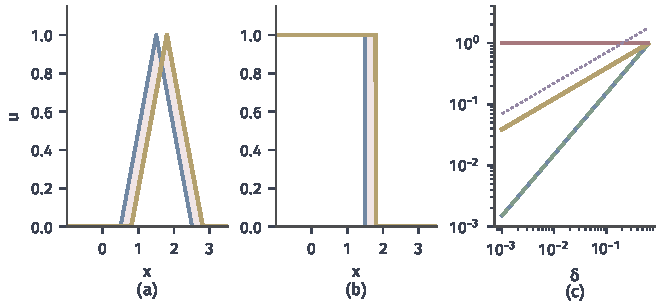
\includegraphics[width=112mm]{figures/06-differential-equations/02-partial-differential-equations/matplotlib/transp-velocity-perturb/figure.pdf}
  \caption{$v=1$（蓝）与$v=1+\delta$（黄）的解，$t=1.5$，$\delta=0.2$，浅红区域是两解的差。(a)三角形初值。(b)台阶初值。(c)误差随$\delta$的变化（对数坐标）：蓝线是三角形的一致误差，与绿色虚线（台阶的$L^{1}$误差）重合，都正比于$\delta$；黄线是台阶的$L^{2}$误差，与紫色点线（参考斜率$1/2$）平行；红线是台阶的一致误差。}
  \label{fig:transp-velocity-perturb}
\end{BookInlineFigure}

式~\eqref{eq:transp-step-lp}的收敛率$1/p$比光滑情形的一阶要慢，$p=2$时只有$1/2$阶。对一般的$L^{p}$初值，收敛仍然成立，只是不再有统一的速率。

\begin{theorem}[粗糙初值的$L^{p}$收敛]
\label{thm:transp-lp-convergence}
设$\bm{v}^{n},\bm{v}$满足条件（V），常数$L$相同，$\nabla\cdot\bm{v}^{n},\nabla\cdot\bm{v}\leq\kappa$，且$\bm{v}^{n}$在$\mathbb{R}^{d}\times[0,T]$上一致收敛于$\bm{v}$。设$u_0\in L^{p}(\mathbb{R}^{d})$，$1\leq p<\infty$，$u^{n},u$是相应的解$u_0\circ\bm{\varphi}^{n}_{t,0}$与$u_0\circ\bm{\varphi}_{t,0}$。则对每个$t\in[0,T]$，
\begin{equation}
  \lVert u^{n}(\cdot,t)-u(\cdot,t)\rVert_{p}\to0.
  \label{eq:transp-lp-convergence}
\end{equation}
\end{theorem}

\begin{proof}
任取$\varepsilon>0$。Lipschitz紧支函数在$L^{p}$中稠密，取这样的$w$，使$\lVert u_0-w\rVert_{p}<\varepsilon$，它的支集在球$B$内，Lipschitz常数为$L_w$。三角不等式给出
\[
  \lVert u^{n}-u\rVert_{p}\leq\lVert(u_0-w)\circ\bm{\varphi}^{n}_{t,0}\rVert_{p}
  +\lVert w\circ\bm{\varphi}^{n}_{t,0}-w\circ\bm{\varphi}_{t,0}\rVert_{p}
  +\lVert(w-u_0)\circ\bm{\varphi}_{t,0}\rVert_{p}.
\]

由定理~\ref{thm:transp-lp}的证明，第一项和第三项都不超过$\mathrm{e}^{\kappa t/p}\varepsilon$。第二项中，定理~\ref{thm:transp-velocity}的第一步给出逐点差不超过$L_wE_n$，其中$E_n\to0$。

被积函数只在$\bm{\varphi}^{n}_{0,t}(B)\cup\bm{\varphi}_{0,t}(B)$上非零，这个集合的体积不超过$2\mathrm{e}^{\kappa t}\lvert B\rvert$，所以第二项不超过
\[
  L_wE_n\bigl(2\mathrm{e}^{\kappa t}\lvert B\rvert\bigr)^{1/p}\to0.
\]
先让$n\to\infty$，再让$\varepsilon\to0$，即得式~\eqref{eq:transp-lp-convergence}。
\end{proof}

定理中$p<\infty$是必需的：式~\eqref{eq:transp-step-sup}就是$p=\infty$的反例。$\varepsilon$的取法依赖$u_0$，所以这里没有速率，这也是间断初值与Lipschitz初值的根本差别。

\paragraph{弱收敛}
数据本身的扰动也可能只在弱意义下小。比如$u_0^{n}(x)=\sin(nx)$在$L^{2}$的有界区间上弱收敛于$0$，但它的$L^{2}$范数不趋于零。

固定速度场，$u_0^{n}\rightharpoonup u_0$（$L^{p}$中弱收敛，$1<p<\infty$）时，对任意$h\in C_c(\mathbb{R}^{d})$，由换元，
\[
  \int u^{n}(\bm{y},t)h(\bm{y})\,\mathrm{d}\bm{y}
  =\int u_0^{n}(\bm{x})\,h\bigl(\bm{\varphi}_{0,t}(\bm{x})\bigr)J_{0,t}(\bm{x})\,\mathrm{d}\bm{x}.
\]

右端的$h(\bm{\varphi}_{0,t}(\cdot))J_{0,t}$是一个固定的$L^{p'}$函数，所以它收敛到对应$u_0$的值。这说明解的弱收敛可以从初值传递过来，但它不提供任何一致的误差估计。上面的振荡初值在$v=x$下的解是$\sin(nx\mathrm{e}^{-t})$，它的振幅始终是$1$，只是积分平均趋于零。

\section{本章小结}
\label{sec:transp-summary}

本章从一个问题出发：给定速度场，一滴墨水此后会怎样？答案取决于要问的量。若问粒子携带的值，它沿轨迹不变；若问单位体积的质量，它要除以流动带来的体积倍率。

两种量都通过同一组对象计算。轨迹由常微分方程$\dot{\bm{x}}=\bm{v}(\bm{x},t)$给出，把所有轨迹放在一起得到流映射$\bm{\varphi}_{s,t}$。场值的解是初值与逆流映射的复合，加上沿轨迹累积的源项；密度的解还要多除一个Jacobian行列式$J_{0,t}$，它由速度的散度沿轨迹积分得到。表~\ref{tab:transp-value-density}给出了两者的对比。

这些结论都有明确的条件。

\begin{itemize}
  \item 条件（V）保证了过每一点恰有一条特征线，逆映射在全空间存在。轨迹爆炸时，解只在流映射的值域上有定义；轨迹不唯一时，反向追踪的结果不确定，$C^{1}$解可能不存在。
  \item 总质量守恒需要闭区域、无源项，或全空间上足够的衰减。沿轨迹的密度不变是另一个结论，它只在无散度时成立。
  \item 经典解要求初值$C^{1}$，连续性方程的经典解还要求$\nabla\cdot\bm{v}$对$\bm{x}$连续可微。折角和间断用弱形式处理，弱形式下的存在和唯一仍然要靠条件（V），粗糙速度场下可能出现集中或非唯一。
  \item 数据误差的$L^{p}$放大由体积膨胀控制，速度误差的$L^{\infty}$估计需要初值和源项的Lipschitz常数。间断初值下一致估计失效，只能用$L^{p}$或弱收敛的语言。
\end{itemize}

这一切都有一个共同的前提：速度场是事先给定的，特征线彼此不相交。若传播速度依赖未知量本身，不同高度的点走得快慢不同，特征线就可能相交，解在有限时间内失去光滑性。第~\ref{chap:scalar-conservation-laws}章讨论这种情形。


\chapter{标量守恒律}
\label{chap:scalar-conservation-laws}

一条单行道上，前方路段车少、车开得快，后方路段车多、车开得慢。密度的分布会怎样随时间变化？第~\ref{chap:transport-equations}章的速度场是事先给定的，墨水只管被水流带走。车流不同：每辆车的速度取决于周围的密度，而密度又取决于所有车的位置。传播速度依赖未知量本身，这一点改变了全部局面。

最直接的后果是波形会变形。以一维Burgers方程为例，它的传播速度就等于场值：高处跑得快，低处跑得慢。高处从后面追上低处，波形的前沿越来越陡，到某一时刻斜率变成无穷，而场值始终有界。微分方程在这一刻失去了逐点的意义，路上的车却不会消失，区间内车辆总数的收支账依然成立。

于是要回到积分形式的收支平衡，并允许解带有间断。这一放宽有代价：同一个初值可以有无穷多个满足收支平衡的解，其中一个甚至让静止的流体自发运动起来。只算总账无法决定解，还需要一条规则来判定信息的传播方向。

本章沿着Burgers方程一路走下去。先用特征线算出光滑解何时失效，再写出允许间断的解和间断的传播速度，接着看选择规则怎样淘汰多余的解。把这些放到左右两个常状态的初值上，可以手算出两种基本的波。最后证明两个合乎规则的解的积分距离不会随时间增大，唯一性由此而来。

\section{守恒律问题}
\label{sec:cons-problem}

一段路上的车辆数只会因为有车从两端进出而改变。把这句话写成数学，就得到本章的方程。

\paragraph{从区间收支到方程}
设$u(x,t)$是$t$时刻$x$处的密度，例如单位长度上的车辆数。单位时间内向右穿过$x$点的量称为\term{通量}（flux）。本章假设通量只通过密度依赖位置和时间，写成$F(u(x,t))$，其中$F:\mathbb{R}\to\mathbb{R}$是给定的函数。

任取区间$[a,b]$，如图~\ref{fig:cons-balance}。区间内的总量只因两端的进出而变化，左端流入，右端流出：
\begin{equation}
  \frac{\mathrm{d}}{\mathrm{d}t}\int_a^b u(x,t)\,\mathrm{d}x=F(u(a,t))-F(u(b,t)).
  \label{eq:cons-balance}
\end{equation}

\begin{BookInlineFigure}
  \centering
  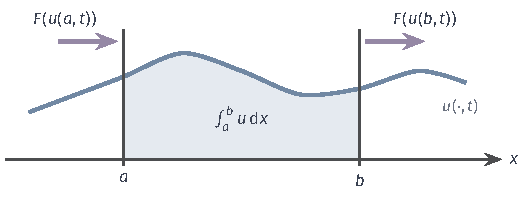
\includegraphics[width=89.8mm]{figures/06-differential-equations/02-partial-differential-equations/tikz/cons-balance/figure.pdf}
  \caption{区间上的收支。蓝线是某一时刻的密度$u(\cdot,t)$，浅蓝区域的面积是区间$[a,b]$内的总量。紫色箭头表示穿过两个端点的通量，左端流入增加总量，右端流出减少总量。}
  \label{fig:cons-balance}
\end{BookInlineFigure}

式~\eqref{eq:cons-balance}没有对$x$求导，也不要求$u$连续，只要积分和端点值有意义就能写出来。后面处理间断时正要回到这一点。现在先假设$u$和$F$都是$C^1$的，把右端写成$\partial_xF(u)$的积分：
\[
  \int_a^b\bigl(\partial_tu+\partial_xF(u)\bigr)\,\mathrm{d}x=0 .
\]

区间$[a,b]$是任取的，被积函数又连续。如果被积函数在某一点不为零，在该点附近的小区间上积分就不为零，与上式矛盾。于是得到
\begin{equation}
  \partial_tu+\partial_xF(u)=0,\qquad x\in\mathbb{R},\ t>0.
  \label{eq:cons-law}
\end{equation}

再给定初始分布
\begin{equation}
  u(x,0)=u_0(x),\qquad x\in\mathbb{R},
  \label{eq:cons-initial}
\end{equation}
式~\eqref{eq:cons-law}与~\eqref{eq:cons-initial}合起来就是\term{标量守恒律}（scalar conservation law）的初值问题。“守恒”一词来自式~\eqref{eq:cons-balance}：若$u$在无穷远处衰减，使两端的通量趋于同一个值，令$a\to-\infty$、$b\to\infty$，则右端为零，全直线上的总量$\int_{\mathbb{R}}u\,\mathrm{d}x$不随时间变化。

\paragraph{通量决定传播速度}
$C^1$解可以用链式法则展开$\partial_xF(u)$，得到
\begin{equation}
  \partial_tu+F'(u)\,\partial_xu=0.
  \label{eq:cons-quasilinear}
\end{equation}

把它与第~\ref{chap:transport-equations}章的输运方程$\partial_tu+v\,\partial_xu=0$对照，形式完全相同，只是速度$v$换成了$F'(u)$。$F'(u)$是密度$u$上的小扰动的传播速度。差别在于，输运方程的$v$事先已知，这里的速度要等解出$u$之后才知道。下面三种通量显示了通量形状带来的不同，见图~\ref{fig:cons-fluxes}。

\begin{itemize}
  \item 线性通量$F(u)=cu$：速度$F'(u)=c$是常数，方程退回到恒定速度的输运方程。
  \item \term{Burgers方程}（Burgers equation）的通量$F(u)=u^2/2$：速度$F'(u)=u$，场值本身就是传播速度。可以把$u$想成一维粒子各自的速度，每个粒子不受力，匀速前进。
  \item 车流通量$F(u)=u(1-u)$，其中$u\in[0,1]$是归一化密度：车速为$1-u$，空路上最快，堵死时为零，流量等于密度乘车速。
\end{itemize}

\begin{BookInlineFigure}
  \centering
  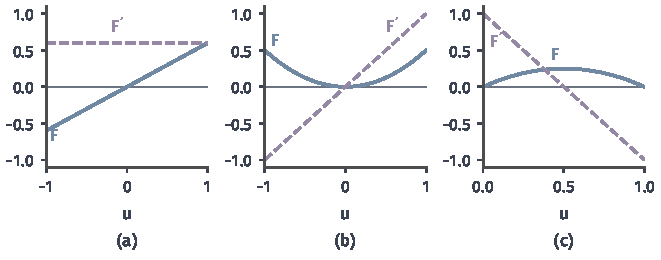
\includegraphics[width=112mm]{figures/06-differential-equations/02-partial-differential-equations/matplotlib/cons-fluxes/figure.pdf}
  \caption{三种通量及其传播速度。蓝色实线是通量$F$，紫色虚线是传播速度$F'$。(a)线性通量$F=0.6u$，速度为常数。(b)Burgers通量$F=u^2/2$，速度等于$u$，$F$是凸函数。(c)车流通量$F=u(1-u)$，速度$1-2u$随密度减小，$F$是凹函数。}
  \label{fig:cons-fluxes}
\end{BookInlineFigure}

车流的例子说明，扰动的传播速度和粒子的速度是两回事。取$u=3/4$，每辆车以速度$1-u=1/4$向前开，而密度扰动的传播速度是
\[
  F'(3/4)=1-2\cdot\frac34=-\frac12 ,
\]
它是负的。车在向前走，密度的变化却向后传，这就是堵车的尾部向后蔓延的原因。Burgers方程里两者恰好相同，读图和手算都最简单，所以本章用
\begin{equation}
  \partial_tu+\partial_x\Bigl(\frac{u^2}{2}\Bigr)=0
  \label{eq:cons-burgers}
\end{equation}
作贯穿全章的例子。

\paragraph{讨论的范围}
本章只讨论一维标量方程。未知量是向量的守恒律系统有多族速度不同的波，它们彼此耦合，本章后面的唯一性论证没有对应物。多维标量方程的熵解理论仍然成立，但间断不再是一条曲线，左右两侧的次序也不复存在，一维的显式构造不能照搬。下文的条件和结论都只针对一维标量问题。


\section{光滑解的失效}
\label{sec:cons-breakdown}

光滑解能活多久？特征线法可以回答这个问题：沿某条曲线把偏微分方程化成常微分方程。与第~\ref{chap:transport-equations}章的差别只在于曲线的速度依赖解。先假设$C^1$解存在，看它必须长什么样。

\paragraph{特征线是直线}
设$F\in C^2$，$u$是式~\eqref{eq:cons-law}的$C^1$解。从初始线上的点$(x_0,0)$出发，解常微分方程
\[
  x'(t)=F'\bigl(u(x(t),t)\bigr),\qquad x(0)=x_0 .
\]

沿这条曲线对$u$求导，再用式~\eqref{eq:cons-quasilinear}，得到
\[
  \frac{\mathrm{d}}{\mathrm{d}t}u(x(t),t)
  =\partial_tu+x'(t)\,\partial_xu
  =\partial_tu+F'(u)\,\partial_xu=0 .
\]

所以$u$沿曲线不变，始终等于$u_0(x_0)$。这样一来$x'(t)=F'(u_0(x_0))$是常数，曲线是一条直线。记
\begin{equation}
  a(x_0)=F'(u_0(x_0)),\qquad X_t(x_0)=x_0+a(x_0)\,t ,
  \label{eq:cons-characteristic}
\end{equation}
这些直线就是\term{特征线}（characteristic curve），$a(x_0)$是它的速度。解沿特征线保持常值：
\begin{equation}
  u\bigl(X_t(x_0),t\bigr)=u_0(x_0).
  \label{eq:cons-implicit}
\end{equation}

Burgers方程的$a=u_0$，特征线为$x=x_0+u_0(x_0)t$。下面的例子贯穿全章：
\begin{equation}
  u_0(x)=\frac{1}{1+x^2}.
  \label{eq:cons-bump}
\end{equation}

图~\ref{fig:cons-speed-arrows}把这条特征线翻译成波形的运动：曲线上的每个点水平移动，移动距离等于自己的高度。峰顶$x_0=0$、$u=1$的点在$t=1$移到$x=1$。右侧$x_0=2$、$u=1/5$的点只移到$x=2.2$。峰的右侧高处追赶低处，波形变陡；左侧高处离开低处，波形变缓。

\begin{BookInlineFigure}
  \centering
  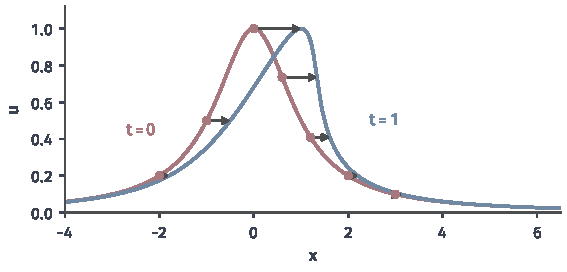
\includegraphics[width=96mm]{figures/06-differential-equations/02-partial-differential-equations/matplotlib/cons-speed-arrows/figure.pdf}
  \caption{Burgers方程中波形的水平移动。红线是初值~\eqref{eq:cons-bump}，红点是几个初始点，黑色箭头的长度等于该点的高度，蓝线是$t=1$的波形。峰的右侧被压陡，左侧被拉缓。}
  \label{fig:cons-speed-arrows}
\end{BookInlineFigure}

\paragraph{特征线相交与斜率爆炸}
斜率会变成多大？对式~\eqref{eq:cons-implicit}关于$x_0$求导，利用$\partial_{x_0}X_t=1+a'(x_0)t$，得到
\[
  \partial_xu\bigl(X_t(x_0),t\bigr)\,\bigl(1+a'(x_0)\,t\bigr)=u_0'(x_0).
\]

除过去，就是沿特征线的斜率公式：
\begin{equation}
  \partial_xu\bigl(X_t(x_0),t\bigr)=\frac{u_0'(x_0)}{1+a'(x_0)\,t}.
  \label{eq:cons-gradient}
\end{equation}

分母有直接的几何含义。$a'(x_0)$度量相邻特征线的速度差，两条相邻特征线的间距按因子$1+a'(x_0)t$变化。$a'<0$时，后面的特征线比前面的快，间距不断缩小；到$t=-1/a'(x_0)$，间距缩成零，分母为零，斜率发散。$a'>0$时间距增大，斜率随时间衰减。

在图~\ref{fig:cons-char-bump}中，初值峰右侧出发的特征线彼此靠拢，红色曲线是它们的包络，包络的尖点就是最早相交的位置。下面的例子算出这个点。

\begin{BookInlineFigure}
  \centering
  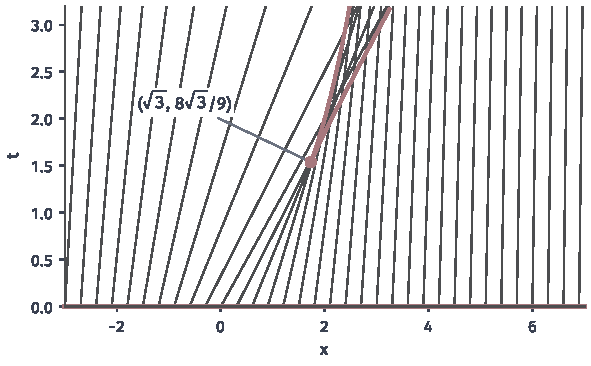
\includegraphics[width=100mm]{figures/06-differential-equations/02-partial-differential-equations/matplotlib/cons-char-bump/figure.pdf}
  \caption{初值~\eqref{eq:cons-bump}的特征线（深灰）。红色粗线是初始线，红色曲线是特征线的包络$t=-1/u_0'(x_0)$，$x=x_0+u_0(x_0)t$，它的尖点（红点）是特征线最早相交的位置。}
  \label{fig:cons-char-bump}
\end{BookInlineFigure}

\begin{example}[最早的相交点]
Burgers方程的$a=u_0$，取初值~\eqref{eq:cons-bump}。分母最早为零的特征线，出发点使$u_0'$最负。求导得
\[
  u_0'(x)=-\frac{2x}{(1+x^2)^2},\qquad u_0''(x)=\frac{6x^2-2}{(1+x^2)^3}.
\]

令$u_0''=0$，在$x>0$一侧得到$x_0=1/\sqrt{3}$。在这一点，
\[
  u_0(x_0)=\frac34,\qquad u_0'(x_0)=-\frac{2/\sqrt{3}}{(4/3)^2}=-\frac{3\sqrt{3}}{8}.
\]

于是最早的相交时刻和位置是
\[
  T^{*}=-\frac{1}{u_0'(x_0)}=\frac{8\sqrt{3}}{9}\approx1.54,\qquad
  x^{*}=x_0+\frac34T^{*}=\sqrt{3}.
\]
\end{example}

\paragraph{光滑解的寿命}
上面的计算是在假设解存在的前提下进行的。下面的定理确切地说明：相交时刻之前解存在且唯一，到了相交时刻不能再以$C^1$的方式继续。

\begin{theorem}[光滑解的寿命]
\label{thm:cons-lifespan}
设$F\in C^2(\mathbb{R})$，$u_0\in C^1(\mathbb{R})$，$u_0$与$u_0'$有界。记$a=F'\circ u_0$，$m=\inf_{\mathbb{R}}a'$。
\begin{enumerate}
  \item 若$m\geq0$，问题~\eqref{eq:cons-law}、\eqref{eq:cons-initial}在$\mathbb{R}\times[0,\infty)$上有唯一的$C^1$解。
  \item 若$m<0$，令
  \begin{equation}
    T^{*}=-\frac{1}{m},
    \label{eq:cons-breaking-time}
  \end{equation}
  此时问题在时间段$[0,T^{*})$上有唯一的$C^1$解，解的值保持在$[\inf u_0,\sup u_0]$内。当$t\uparrow T^{*}$时，$\sup_x\lvert\partial_xu(x,t)\rvert\to\infty$。对任何$T>T^{*}$，$\mathbb{R}\times[0,T]$上不存在$C^1$解；若下确界$m$在某点取到，$T=T^{*}$时同样不存在。
\end{enumerate}
\end{theorem}

\begin{proof}
记$T_0=\infty$（$m\geq0$时）或$T_0=T^{*}$（$m<0$时）。先看映射$X_t$。对$0\leq t<T_0$，
\[
  \partial_{x_0}X_t=1+a'(x_0)\,t\geq1+\min(m,0)\,t>0 .
\]
导数有正的下界，所以$X_t$严格递增，且把$\mathbb{R}$映满$\mathbb{R}$，是$C^1$同胚。

唯一性：设$u$是$\mathbb{R}\times[0,T_0)$上的$C^1$解。前面已经说明，$u$沿式~\eqref{eq:cons-characteristic}的直线不变。这些直线在$t$时刻覆盖整条实轴，所以$u$的值被式~\eqref{eq:cons-implicit}完全确定。

存在性：令$\xi(x,t)$是方程$X_t(\xi)=x$的解。由隐函数定理，$\xi\in C^1$，并且
\[
  \partial_x\xi=\frac{1}{1+a'(\xi)\,t},\qquad
  \partial_t\xi=-\frac{a(\xi)}{1+a'(\xi)\,t}.
\]

定义$u(x,t)=u_0(\xi(x,t))$。它在$t=0$取$u_0$，并且$F'(u)=a(\xi)$，所以
\[
  \partial_tu+F'(u)\,\partial_xu
  =u_0'(\xi)\bigl(\partial_t\xi+a(\xi)\,\partial_x\xi\bigr)=0 .
\]
第一条结论与第二条的存在性就此成立。$u$的值都是$u_0$的值，所以落在$[\inf u_0,\sup u_0]$内。

斜率发散：设$m<0$。取点列$x_n$使$a'(x_n)\to m$。记$C=\max\lvert F''\rvert$，最大值取在$u_0$值域的闭包上，它是紧集，且$C>0$（否则$a'\equiv0$）。由$a'=F''(u_0)u_0'$，当$n$充分大时
\[
  \lvert u_0'(x_n)\rvert\geq\frac{\lvert a'(x_n)\rvert}{C}\geq\frac{\lvert m\rvert}{2C}.
\]

对固定的$t<T^{*}$，有$1+mt>0$，且$n\to\infty$时$1+a'(x_n)t\to1+mt$。取$n$充分大，使$1+a'(x_n)t\leq2(1+mt)$，由式~\eqref{eq:cons-gradient}，
\[
  \sup_x\lvert\partial_xu(x,t)\rvert\geq\frac{\lvert m\rvert}{4C\,(1+mt)}.
\]
令$t\uparrow T^{*}$，右端趋于无穷。

不可延拓：设$u$是$\mathbb{R}\times[0,T]$上的$C^1$解，$T>T^{*}$。由$m<-1/T$，存在$x_0$使$a'(x_0)<-1/T$；若下确界在某点取到且$T=T^{*}$，就取该点。令$t_1=-1/a'(x_0)\in(0,T]$，此时$a'(x_0)\neq0$，从而$u_0'(x_0)\neq0$。

前面的推导对解存在的整个时间段成立，于是在$t=t_1$时
\[
  \partial_xu\bigl(X_{t_1}(x_0),t_1\bigr)\,\bigl(1+a'(x_0)\,t_1\bigr)=u_0'(x_0).
\]
左端的第二个因子为零，右端不为零，矛盾。
\end{proof}

对Burgers方程，$a'=u_0'$，$T^{*}=-1/\inf u_0'$。特别地，有界的$C^1$初值（导数有界）给出整体$C^1$解，当且仅当$u_0$单调不减。定理中的条件各有作用：$u_0'$有界保证$m$有限，否则$T^{*}$可以为零；$F''$非零才让速度随$u$变化，线性通量的$a'\equiv0$，永远不会相交。

有界性和光滑性是分开的两件事。第~\ref{chap:ordinary-differential-equations}章的爆炸是解的值趋于无穷；这里相反，解的值始终在初值范围内，发散的是导数。图~\ref{fig:cons-gradient-blowup}显示，初值~\eqref{eq:cons-bump}的压缩侧斜率在$T^{*}$发散，膨胀侧斜率逐渐衰减，而最大值始终为$1$。

\begin{BookInlineFigure}
  \centering
  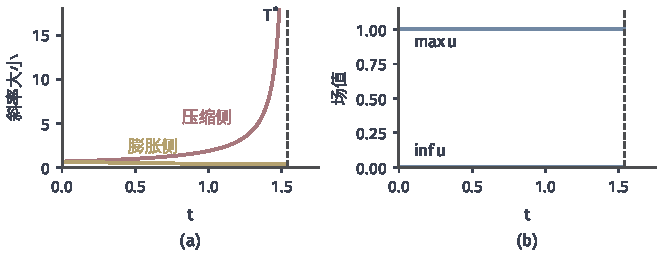
\includegraphics[width=112mm]{figures/06-differential-equations/02-partial-differential-equations/matplotlib/cons-gradient-blowup/figure.pdf}
  \caption{初值~\eqref{eq:cons-bump}的斜率与场值。(a)红线是压缩侧的最大下降斜率$\max_{x_0}(-u_0'/(1+tu_0'))$，黄线是膨胀侧的最大上升斜率，虚线是$T^{*}$。(b)场值的上界和下确界（蓝）不随时间变化。}
  \label{fig:cons-gradient-blowup}
\end{BookInlineFigure}

\paragraph{相交之后发生了什么}
定理说的是映射$X_t$的单调性。图~\ref{fig:cons-fold-map}画出$x_0\mapsto X_t(x_0)$在三个时刻的形状：$T^{*}$之前严格递增，$T^{*}$时出现水平切点，之后出现折叠，同一个$x$有三个原像，也就是有三条特征线到达同一点，各自带来不同的值。

\begin{BookInlineFigure}
  \centering
  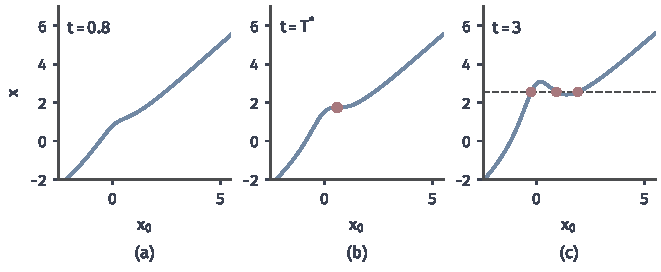
\includegraphics[width=112mm]{figures/06-differential-equations/02-partial-differential-equations/matplotlib/cons-fold-map/figure.pdf}
  \caption{初值~\eqref{eq:cons-bump}的映射$X_t$。(a)$t=0.8$，严格递增。(b)$t=T^{*}$，红点是水平切点$(1/\sqrt{3},\sqrt{3})$。(c)$t=3$，映射折叠，虚线$x=2.55$与曲线有三个交点（红点）。}
  \label{fig:cons-fold-map}
\end{BookInlineFigure}

把折叠的结果画成波形，就是图~\ref{fig:cons-steepening}(b)：曲线翻转，成为多值的。水面的波可以卷起来，同一个$x$上有几层水；密度却不能，同一时刻同一地点只有一个车流密度。所以$T^{*}$之后，式~\eqref{eq:cons-implicit}不再给出一个函数。

\begin{BookInlineFigure}
  \centering
  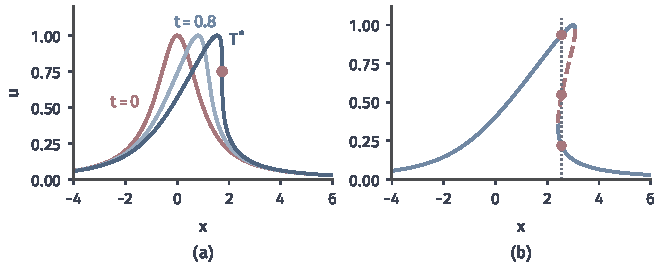
\includegraphics[width=112mm]{figures/06-differential-equations/02-partial-differential-equations/matplotlib/cons-steepening/figure.pdf}
  \caption{波形的变陡与翻转。(a)红线是$t=0$，蓝色由浅到深是$t=0.8$和$t=T^{*}$，红点是斜率首次为无穷的位置$(\sqrt{3},3/4)$。(b)$t=3$时沿特征线算出的图像，红色虚线是翻转部分，竖直点线$x=2.55$上有三个值。}
  \label{fig:cons-steepening}
\end{BookInlineFigure}

第~\ref{chap:transport-equations}章的轨迹不会相交，原因是给定的Lipschitz速度场让常微分方程的解唯一，两条轨迹不能在同一时刻到达同一点。这里两条特征线到达同一点时带着不同的场值，也就有不同的速度，它们不是同一个速度场下的轨迹，唯一性定理管不到它们。速度依赖解，正是相交的来源。

\paragraph{斜坡：所有特征线同时汇聚}
还有一个算起来更简单的初值：
\begin{equation}
  u_0(x)=\begin{cases}1,&x<0,\\1-x,&0\leq x\leq1,\\0,&x>1.\end{cases}
  \label{eq:cons-ramp}
\end{equation}

它只是Lipschitz连续，但沿特征线的计算不受影响。在$(0,1)$上$a'=-1$，从那里出发的特征线$x=x_0+(1-x_0)t$全部在$(1,1)$汇聚，$T^{*}=1$。反解出$x_0=(x-t)/(1-t)$，得到$t<1$时的解
\begin{equation}
  u(x,t)=\frac{1-x}{1-t},\qquad t\leq x\leq1,
  \label{eq:cons-ramp-solution}
\end{equation}
其余区域取常值$1$或$0$。第~\ref{sec:cons-weak}节将接着算出$t>1$时的解，这时解必须带一个间断。


\section{弱解}
\label{sec:cons-weak}

特征线在$T^{*}$失效，收支平衡并没有失效。路上的车不会因为斜率变成无穷而消失，式~\eqref{eq:cons-balance}依然有意义。我们需要一种不依赖导数的方式说出“解满足方程”，并回答间断会以多快的速度移动。

\subsection{积分守恒}
\label{subsec:cons-integral}

把式~\eqref{eq:cons-balance}对时间从$t_1$积分到$t_2$，得到时空矩形上的收支账：
\begin{equation}
  \begin{aligned}
    &\int_a^b u(x,t_2)\,\mathrm{d}x-\int_a^b u(x,t_1)\,\mathrm{d}x\\
    &\qquad+\int_{t_1}^{t_2}F(u(b,t))\,\mathrm{d}t
    -\int_{t_1}^{t_2}F(u(a,t))\,\mathrm{d}t=0 .
  \end{aligned}
  \label{eq:cons-box}
\end{equation}

图~\ref{fig:cons-box}把四项画在$(x,t)$平面上：矩形的上下两边记录总量，左右两边记录流过的量。把$(F(u),u)$看成$(x,t)$平面上的向量场，式~\eqref{eq:cons-box}说的是这个场穿过矩形边界的净通量为零。间断线可以从矩形中穿过，这四项仍然都有意义。

\begin{BookInlineFigure}
  \centering
  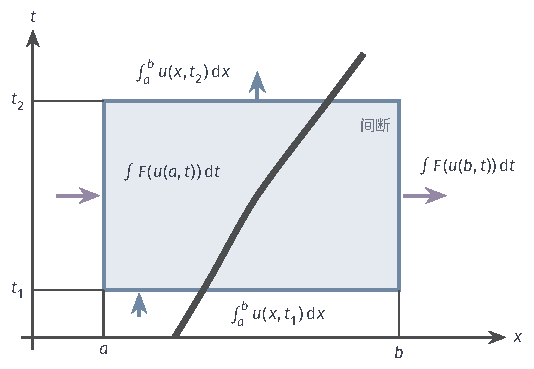
\includegraphics[width=90.4mm]{figures/06-differential-equations/02-partial-differential-equations/tikz/cons-box/figure.pdf}
  \caption{时空矩形上的收支。上下两边的蓝色箭头记录$t_2$、$t_1$时刻区间内的总量，左右两边的紫色箭头记录时段内流入、流出的量。深灰粗线是一条间断线，它穿过矩形时四项仍有定义。}
  \label{fig:cons-box}
\end{BookInlineFigure}

\paragraph{用光滑权重代替矩形}
用矩形检验有两点不便：它要用到$u$在线段上的值，而$u$只是有界可测时这样的值没有确切含义；矩形的边角也不便做微积分。办法是把矩形的示性函数换成光滑的权重$\varphi$，如图~\ref{fig:cons-test-weight}。这就像用一个边缘柔和的窗口观察收支，$\varphi$在窗口内部几乎是常数，它的导数集中在边缘附近，而边缘正是收支发生的地方。

\begin{BookInlineFigure}
  \centering
  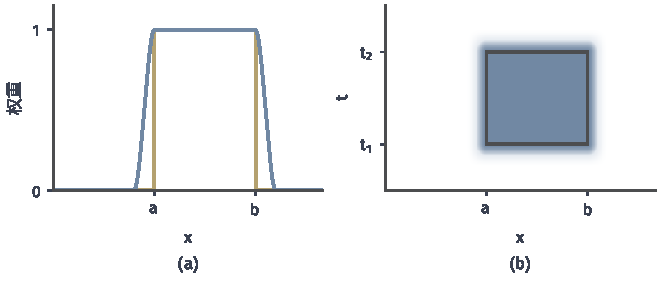
\includegraphics[width=112mm]{figures/06-differential-equations/02-partial-differential-equations/matplotlib/cons-test-weight/figure.pdf}
  \caption{用光滑权重代替矩形。(a)一维剖面：黄线是示性函数，蓝线是光滑的近似。(b)时空平面上的权重$\varphi$，颜色越深值越大，黑框是矩形$[a,b]\times[t_1,t_2]$。$\varphi$的导数只在黑框附近不为零。}
  \label{fig:cons-test-weight}
\end{BookInlineFigure}

设$u$是$C^1$解，$\varphi\in C_c^{\infty}(\mathbb{R}\times[0,\infty))$是\term{测试函数}（test function）。它在$t=0$可以不为零，在大的$\lvert x\rvert$和$t$上为零。把式~\eqref{eq:cons-law}乘以$\varphi$再积分：
\[
  \int_0^{\infty}\!\!\int_{\mathbb{R}}\bigl(\partial_tu+\partial_xF(u)\bigr)\varphi\,\mathrm{d}x\,\mathrm{d}t=0 .
\]

对$t$分部积分时，下限$t=0$留下一项$-\int_{\mathbb{R}}u_0\,\varphi(\cdot,0)\,\mathrm{d}x$；对$x$分部积分没有边界项。所有导数都转到$\varphi$上之后，得到下面的定义。

\begin{definition}[弱解]
\label{def:cons-weak-solution}
设$u_0\in L^{\infty}(\mathbb{R})$，$F\in C^1(\mathbb{R})$。有界可测函数$u$称为问题~\eqref{eq:cons-law}、\eqref{eq:cons-initial}的\term{弱解}（weak solution），若对每个$\varphi\in C_c^{\infty}(\mathbb{R}\times[0,\infty))$，
\begin{equation}
  \int_0^{\infty}\!\!\int_{\mathbb{R}}\bigl(u\,\partial_t\varphi+F(u)\,\partial_x\varphi\bigr)\,\mathrm{d}x\,\mathrm{d}t
  +\int_{\mathbb{R}}u_0\,\varphi(\cdot,0)\,\mathrm{d}x=0 .
  \label{eq:cons-weak}
\end{equation}
\end{definition}

式~\eqref{eq:cons-weak}没有$u$的导数，间断的$u$也能代入。初值的进入方式值得留意：$\varphi$在$t=0$不必为零，第二项正是下边界上的收支。若只取在$t=0$附近为零的$\varphi$，初值就看不见了。

取$\varphi$趋于矩形的示性函数，$\partial_t\varphi$在矩形上下边附近集中，$\partial_x\varphi$在左右边附近集中，式~\eqref{eq:cons-weak}的极限就回到式~\eqref{eq:cons-box}，对几乎所有的$a,b,t_1,t_2$成立。弱形式与矩形收支说的是同一件事。

弱解的概念确实推广了经典解，下面的引理说明两者在光滑情形下一致。

\begin{lemma}[经典解与弱解]
\label{lem:cons-classical-weak}
设$u\in C^1(\mathbb{R}\times[0,\infty))$有界，$F\in C^1$，$u_0$连续有界。则$u$是经典解（满足式~\eqref{eq:cons-law}、\eqref{eq:cons-initial}）当且仅当$u$满足式~\eqref{eq:cons-weak}。
\end{lemma}

\begin{proof}
必要性就是上面的分部积分。

充分性：式~\eqref{eq:cons-weak}对$u$反向分部积分。先取在$t=0$附近为零的$\varphi$，得到
\[
  \int_0^{\infty}\!\!\int_{\mathbb{R}}\bigl(\partial_tu+\partial_xF(u)\bigr)\varphi\,\mathrm{d}x\,\mathrm{d}t=0 .
\]
被积函数中的括号连续，若在某点不为零，取该点附近符号一致的$\varphi\geq0$，积分不为零，矛盾。所以式~\eqref{eq:cons-law}处处成立。

再取一般的$\varphi$，反向分部积分后内部的项已经为零，剩下
\[
  \int_{\mathbb{R}}\bigl(u_0-u(\cdot,0)\bigr)\varphi(\cdot,0)\,\mathrm{d}x=0 .
\]
$\varphi(\cdot,0)$可以是任意的$C_c^{\infty}$函数，所以$u(\cdot,0)=u_0$。
\end{proof}

\paragraph{分段满足方程并不够}
弱形式放宽了要求，但并非什么间断都行。取初值$u_0=1$（$x<0$）、$u_0=0$（$x>0$）。候选函数“间断永远不动”，即$u(x,t)=u_0(x)$，在间断线两侧都是常数，逐点满足方程。

用式~\eqref{eq:cons-box}在矩形$[-1,1]\times[0,1]$上算账，见图~\ref{fig:cons-wrong-speed}(a)。区间内的总量两个时刻都是$1$，变化量为零。左端流入$F(1)\cdot1=1/2$，右端流出$F(0)\cdot1=0$，净流入为$1/2$。账对不上，因为流进来的$1/2$没有地方去。

如果间断以速度$1/2$右移，$t=1$时总量变成$3/2$，增加的$1/2$恰好是净流入，账就平了，见图~\ref{fig:cons-wrong-speed}(b)。可见分段满足方程还不够，间断的移动速度必须与流入流出相配。下一小节给出这个条件。

\begin{BookInlineFigure}
  \centering
  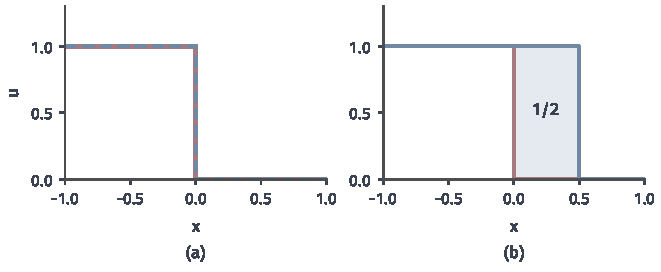
\includegraphics[width=112mm]{figures/06-differential-equations/02-partial-differential-equations/matplotlib/cons-wrong-speed/figure.pdf}
  \caption{间断速度与收支账，初值为左$1$右$0$的阶跃（红），$t=1$时的候选解为蓝线。(a)间断不动：总量不变，净流入的$1/2$无处安放。(b)间断以速度$1/2$右移：浅蓝矩形的面积$1/2$恰好等于净流入。}
  \label{fig:cons-wrong-speed}
\end{BookInlineFigure}

\paragraph{收支账选不出解}
反过来，把收支账算平也未必就够了。取Burgers方程和相反的阶跃：$u_0=0$（$x<0$）、$u_0=1$（$x>0$）。下面两个函数的初值都是这个阶跃：
\[
  u^{\mathrm{j}}(x,t)=\begin{cases}0,&x<t/2,\\1,&x>t/2,\end{cases}\qquad
  u^{\mathrm{f}}(x,t)=\begin{cases}0,&x\leq0,\\x/t,&0<x<t,\\1,&x\geq t.\end{cases}
\]

在矩形$[-2,2]\times[0,1]$上算账。初始总量是$2$，右端流出$F(1)\cdot1=1/2$，左端不流入，所以$t=1$时总量应为$3/2$。对$u^{\mathrm{j}}$，$t=1$时值为$1$的部分长度是$3/2$；对$u^{\mathrm{f}}$，总量是
\[
  \int_0^1x\,\mathrm{d}x+1\cdot1=\frac32 .
\]
两个账都平，差别只是把图~\ref{fig:cons-same-ledger}中两块面积相等的小三角形互换了位置。

\begin{BookInlineFigure}
  \centering
  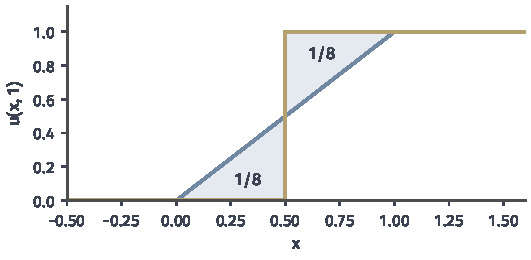
\includegraphics[width=90mm]{figures/06-differential-equations/02-partial-differential-equations/matplotlib/cons-same-ledger/figure.pdf}
  \caption{同一阶跃初值的两个候选解在$t=1$的形状：黄线是带间断的$u^{\mathrm{j}}$，蓝线是连续的$u^{\mathrm{f}}$。两块浅蓝三角形的面积都是$1/8$，一增一减，总量相同。}
  \label{fig:cons-same-ledger}
\end{BookInlineFigure}

矩形收支是必要条件，这里只验证了一个矩形。下一小节的定理会说明这两个函数确实都是弱解。经典解一定满足弱形式，但弱形式可以容许同一个初值有多个解，这是放宽解的概念要付的代价。

\subsection{跳跃条件}
\label{subsec:cons-jump}

间断以多快的速度移动？设间断两侧的状态是$u_-$（左）和$u_+$（右），间断的速度是$s$。

换到跟着间断一起运动的坐标系，见图~\ref{fig:cons-moving-jump}(b)。在这个坐标系里间断静止，所有物质的速度都减去了$s$，通量相应变成$F(u)-su$。间断是一条线，存不下任何东西，所以从左边进入的量必须等于从右边流出的量：
\[
  F(u_-)-s\,u_-=F(u_+)-s\,u_+ .
\]

\begin{BookInlineFigure}
  \centering
  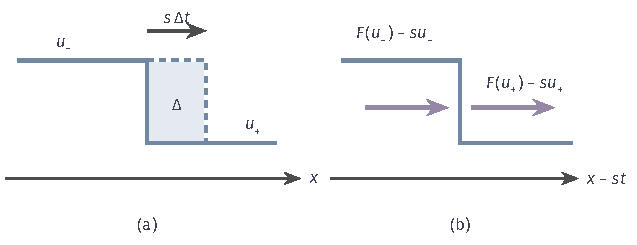
\includegraphics[width=107.9mm]{figures/06-differential-equations/02-partial-differential-equations/tikz/cons-moving-jump/figure.pdf}
  \caption{间断处的收支。(a)实验室坐标：时间$\Delta t$内间断移动$s\Delta t$，浅蓝矩形内的总量变化$(u_--u_+)s\Delta t$必须等于净流入。(b)随间断运动的坐标：相对通量$F(u)-su$在间断两侧相等，紫色箭头表示这两股流量。}
  \label{fig:cons-moving-jump}
\end{BookInlineFigure}

移项就得到\term{Rankine--Hugoniot条件}（Rankine--Hugoniot condition）。下面的定理说明，这个条件恰好刻画了分段光滑函数何时是弱解。

\begin{theorem}[Rankine--Hugoniot条件]
\label{thm:cons-rh}
设$F\in C^1$，$V\subset\mathbb{R}\times(0,\infty)$是开集，$C^1$曲线$x=\gamma(t)$把$V$分成左右两部分$V_-$、$V_+$。设$u$在$V_\pm$内是$C^1$的并满足式~\eqref{eq:cons-law}，$u$及其一阶偏导都能连续延拓到曲线的两侧，单侧极限记为$u_\pm(t)$。则$u$对所有$\varphi\in C_c^{\infty}(V)$满足
\begin{equation}
  \iint_V\bigl(u\,\partial_t\varphi+F(u)\,\partial_x\varphi\bigr)\,\mathrm{d}x\,\mathrm{d}t=0
  \label{eq:cons-rh-weak}
\end{equation}
当且仅当在曲线上
\begin{equation}
  \gamma'(t)\,\bigl(u_+-u_-\bigr)=F(u_+)-F(u_-).
  \label{eq:cons-rh}
\end{equation}
\end{theorem}

\begin{proof}
考虑$(x,t)$平面上的向量场$\bm{W}=(F(u)\varphi,\ u\varphi)$。在$V_\pm$内，利用式~\eqref{eq:cons-law}，
\[
  \nabla_{(x,t)}\cdot\bm{W}=F(u)\,\partial_x\varphi+u\,\partial_t\varphi .
\]

$\varphi$在$V$的边界附近为零，所以在$V_-$上用散度定理时，只有曲线部分有贡献。曲线$x-\gamma(t)=0$上指向$V_+$（即$V_-$的外法向）的方向是$(1,-\gamma')$，弧长元是$\sqrt{1+\gamma'^2}\,\mathrm{d}t$，单位化因子抵消，于是
\[
  \iint_{V_-}\bigl(u\,\partial_t\varphi+F(u)\,\partial_x\varphi\bigr)\,\mathrm{d}x\,\mathrm{d}t
  =\int\bigl(F(u_-)-\gamma'u_-\bigr)\,\varphi(\gamma(t),t)\,\mathrm{d}t .
\]

在$V_+$上外法向反号，得到
\[
  \iint_{V_+}\bigl(u\,\partial_t\varphi+F(u)\,\partial_x\varphi\bigr)\,\mathrm{d}x\,\mathrm{d}t
  =-\int\bigl(F(u_+)-\gamma'u_+\bigr)\,\varphi(\gamma(t),t)\,\mathrm{d}t .
\]

两式相加，积分等式等价于
\[
  \int\Bigl(F(u_-)-F(u_+)-\gamma'(u_--u_+)\Bigr)\,\varphi(\gamma(t),t)\,\mathrm{d}t=0
\]
对所有$\varphi$成立。括号里的函数连续，$\varphi$在曲线上的值可以任取，所以这等价于括号恒为零，即式~\eqref{eq:cons-rh}。
\end{proof}

定理针对$t>0$的内部。若分段$C^1$的$u$在各块上取到相应的初值，边界$t=0$的项恰好给出式~\eqref{eq:cons-weak}中的初值积分，所以$u$是弱解当且仅当每条间断线上式~\eqref{eq:cons-rh}成立。有两个特殊情形要留意。$u_+=u_-$时式~\eqref{eq:cons-rh}自动成立，所以$u$连续、仅导数间断的折线不需要额外条件，前面的$u^{\mathrm{f}}$就属于这种情形。条件的另一面是，它只约束速度，不约束两侧状态的相对大小。

\paragraph{波速是通量的弦斜率}
$u_-\neq u_+$时，式~\eqref{eq:cons-rh}给出
\begin{equation}
  s=\frac{F(u_+)-F(u_-)}{u_+-u_-},
  \label{eq:cons-shock-speed}
\end{equation}
它是通量图像上连接两个状态的弦的斜率，如图~\ref{fig:cons-rh-chord}。由积分中值定理，$s$是$F'$在$u_-$与$u_+$之间的平均值。Burgers方程的弦斜率特别简单：
\begin{equation}
  s=\frac{u_-+u_+}{2}.
  \label{eq:cons-burgers-speed}
\end{equation}
前面的阶跃取$u_-=0$、$u_+=1$，$s=1/2$，所以$u^{\mathrm{j}}$确实是弱解；$u^{\mathrm{f}}$由两条连续接缝组成，也是弱解。一个初值，两个弱解。

\begin{BookInlineFigure}
  \centering
  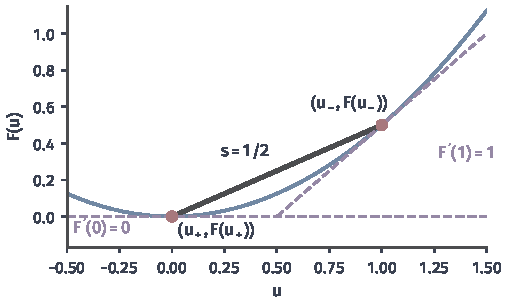
\includegraphics[width=86mm]{figures/06-differential-equations/02-partial-differential-equations/matplotlib/cons-rh-chord/figure.pdf}
  \caption{Rankine--Hugoniot速度的几何含义，$F=u^2/2$（蓝）。两个红点是状态$u_-=1$、$u_+=0$，深灰粗线是弦，斜率$s=1/2$。紫色虚线是两端的切线，斜率$F'(1)=1$与$F'(0)=0$，$s$介于两者之间。}
  \label{fig:cons-rh-chord}
\end{BookInlineFigure}

\paragraph{斜坡初值的后续}
现在可以接着算斜坡~\eqref{eq:cons-ramp}。$t=1$时解变成左$1$右$0$的台阶，位置在$x=1$。此后沿用这个台阶，令间断从$(1,1)$出发，由式~\eqref{eq:cons-burgers-speed}，速度是$1/2$，于是间断线为$x=(1+t)/2$，解为
\begin{equation}
  u(x,t)=\begin{cases}1,&x<(1+t)/2,\\0,&x>(1+t)/2,\end{cases}\qquad t\geq1.
  \label{eq:cons-ramp-shock}
\end{equation}

图~\ref{fig:cons-ramp-shock}(a)中，左侧的特征线以速度$1$从后面追上间断，右侧的特征线停在原地等间断到来，都终止在间断线上。

\begin{BookInlineFigure}
  \centering
  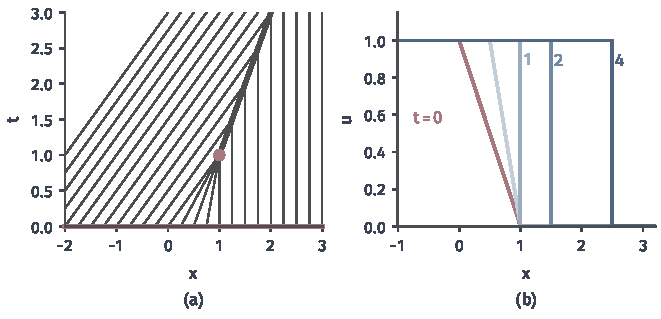
\includegraphics[width=112mm]{figures/06-differential-equations/02-partial-differential-equations/matplotlib/cons-ramp-shock/figure.pdf}
  \caption{斜坡初值的解。(a)特征线（细线）在红点$(1,1)$汇聚，此后深灰粗线$x=(1+t)/2$是间断线，两侧的特征线都在它上面终止。(b)红线是$t=0$，蓝色由浅到深是$t=0.5,1,2,4$。}
  \label{fig:cons-ramp-shock}
\end{BookInlineFigure}

\paragraph{等面积法则}
式~\eqref{eq:cons-ramp-shock}还可以换一个角度得到。沿特征线得到的多值图像虽然不是函数，但曲线下的面积是守恒的。把图像写成参数形式$(x_0+tu_0(x_0),\,u_0(x_0))$，带符号的面积随时间的变化是
\[
  \frac{\mathrm{d}}{\mathrm{d}t}\int u_0\,\bigl(1+t\,u_0'\bigr)\,\mathrm{d}x_0
  =\int u_0\,u_0'\,\mathrm{d}x_0=\Bigl[\frac{u_0^2}{2}\Bigr]_{-\infty}^{\infty},
\]
在初值的两端取相同的极限时为零。要把多值图像截成单值函数并保持总量，就应竖直切一刀，使切掉的两块面积相等，这称为\term{等面积法则}（equal-area rule）。

图~\ref{fig:cons-equal-area}(a)在$t=2$验证这一点。斜坡的多值图像中间一段是从$(1,0)$到$(2,1)$的线段$u=x-1$。在$x=c$处切开，左边多出的三角形面积是$(c-1)^2/2$，右边少掉的三角形面积是$(2-c)^2/2$。令两者相等，得$c=3/2$，与$x=(1+t)/2$在$t=2$的值一致。

\begin{BookInlineFigure}
  \centering
  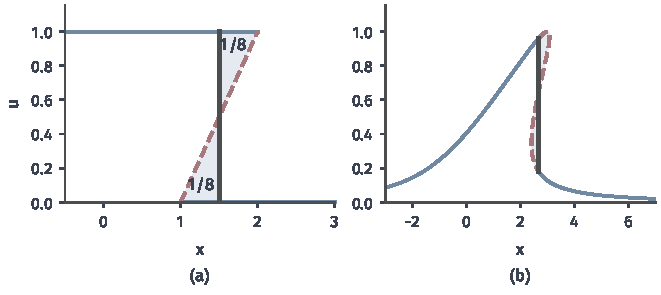
\includegraphics[width=112mm]{figures/06-differential-equations/02-partial-differential-equations/matplotlib/cons-equal-area/figure.pdf}
  \caption{等面积法则。蓝线是单值的解，红色虚线是沿特征线得到的翻转部分，深灰竖线是间断位置，两块浅蓝区域面积相等。(a)斜坡初值在$t=2$，间断位于$x=3/2$，每块面积$1/8$。(b)初值~\eqref{eq:cons-bump}在$t=3$，间断位置由数值积分得到。}
  \label{fig:cons-equal-area}
\end{BookInlineFigure}

贯穿例子~\eqref{eq:cons-bump}的间断路径没有闭式，但可以把上面两条结合起来计算。设$\gamma(t)$是间断位置，$u_\pm$是多值图像在$x=\gamma(t)$处最靠左和最靠右的分支的值，由式~\eqref{eq:cons-burgers-speed}，
\begin{equation}
  \gamma'(t)=\frac{u_-(t)+u_+(t)}{2},\qquad \gamma(T^{*})=\sqrt{3}.
  \label{eq:cons-bump-shock}
\end{equation}

这是一个常微分方程，右端要在每一步解两次特征线方程。数值积分得$\gamma(3)\approx2.677$。图~\ref{fig:cons-bump-shock}(a)中间断从红点长出，特征线不断汇入。(b)显示了波形的演化：间断形成后，峰逐渐被削低，波形的前沿始终保持一个台阶。

\begin{BookInlineFigure}
  \centering
  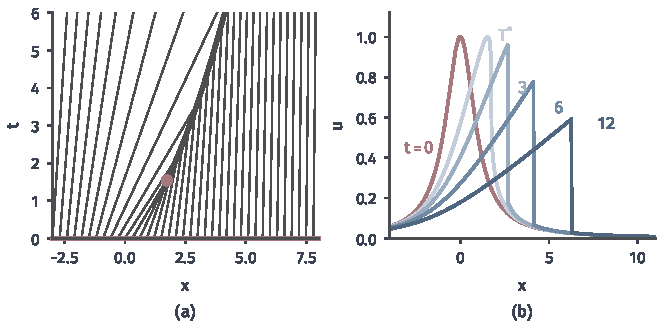
\includegraphics[width=112mm]{figures/06-differential-equations/02-partial-differential-equations/matplotlib/cons-bump-shock/figure.pdf}
  \caption{初值~\eqref{eq:cons-bump}的激波形成之后。(a)细线是特征线，它们都在深灰粗线（数值求解式~\eqref{eq:cons-bump-shock}得到的间断路径）上终止，红点是最早的相交点。(b)红线是$t=0$，蓝色由浅到深是$t=T^{*},3,6,12$，台阶越来越矮。}
  \label{fig:cons-bump-shock}
\end{BookInlineFigure}

\paragraph{同一方程的不同守恒形式}
跳跃条件依赖于哪个量守恒。$C^1$时，Burgers方程乘以$u$，得到同样成立的
\[
  \partial_t\Bigl(\frac{u^2}{2}\Bigr)+\partial_x\Bigl(\frac{u^3}{3}\Bigr)=0 .
\]
两个方程的光滑解完全相同，但把后者看作守恒律时，守恒量是$u^2/2$，通量是$u^3/3$。

对同一组状态$u_-=1$、$u_+=0$，由式~\eqref{eq:cons-shock-speed}，两种写法给出的速度分别是
\[
  s=\frac{1/2-0}{1-0}=\frac12,\qquad
  s=\frac{1/3-0}{1/2-0}=\frac23 .
\]

图~\ref{fig:cons-form-speed}画出这两条路径。所以方程写成哪一种守恒形式不是记号问题，而是在说明哪个量真正守恒；$u\,\partial_xu$这样的非守恒写法在间断处没有定义，也就无从决定速度。

\begin{BookInlineFigure}
  \centering
  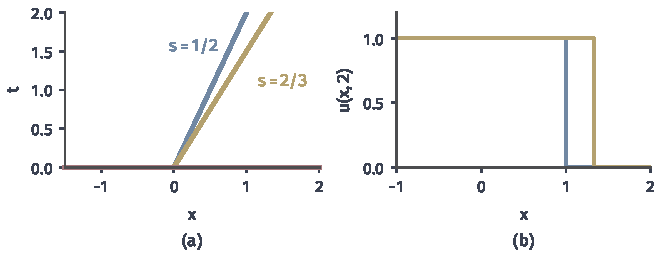
\includegraphics[width=112mm]{figures/06-differential-equations/02-partial-differential-equations/matplotlib/cons-form-speed/figure.pdf}
  \caption{守恒形式决定间断速度，状态$u_-=1$、$u_+=0$。(a)蓝线是以$u$为守恒量得到的路径$s=1/2$，黄线是以$u^2/2$为守恒量得到的路径$s=2/3$。(b)两种情形在$t=2$的形状。}
  \label{fig:cons-form-speed}
\end{BookInlineFigure}

跳跃条件只保证穿过间断的总量收支平衡。$u^{\mathrm{j}}$满足它，$u^{\mathrm{f}}$也满足，所以还要有别的办法检验传播方向是否合理。


\section{熵条件}
\label{sec:cons-entropy}

弱解到底多到什么程度？怎样从中挑出合理的那一个？本节先把多余的解摆出来，再从特征线的方向和小黏性的极限两个角度找到选择规则，最后把规则写成对一切弱解都能检验的不等式。

\paragraph{同一初值的无穷多个弱解}
仍取Burgers方程和阶跃初值$u_0=0$（$x<0$）、$u_0=1$（$x>0$）。上一节的两个解只是一族解的两端。任取$\alpha\in[0,1]$，令
\begin{equation}
  u^{\alpha}(x,t)=\begin{cases}
    0,&x<\alpha t/2,\\
    \alpha,&\alpha t/2<x<\alpha t,\\
    x/t,&\alpha t<x<t,\\
    1,&x\geq t.
  \end{cases}
  \label{eq:cons-weak-family}
\end{equation}

逐块检验。常数块上两个偏导都是零，方程成立；块$u=x/t$上
\[
  \partial_tu+u\,\partial_xu=-\frac{x}{t^2}+\frac{x}{t}\cdot\frac1t=0 .
\]
唯一的跳跃在$x=\alpha t/2$处，两侧是$0$和$\alpha$，由式~\eqref{eq:cons-burgers-speed}，速度应为$\alpha/2$，正好相符。其余两条接缝连续。由定理~\ref{thm:cons-rh}，每个$u^{\alpha}$都是弱解。

图~\ref{fig:cons-weak-family}画出$\alpha=1,\,1/2,\,0$三种情形。$\alpha=1$就是$u^{\mathrm{j}}$，$\alpha=0$就是$u^{\mathrm{f}}$，中间的$\alpha$把一部分扇形换成了向上的跳跃。

\begin{BookInlineFigure}
  \centering
  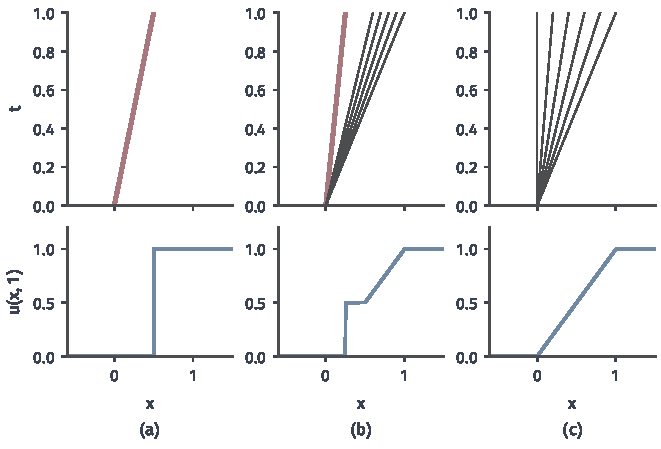
\includegraphics[width=112mm]{figures/06-differential-equations/02-partial-differential-equations/matplotlib/cons-weak-family/figure.pdf}
  \caption{阶跃初值的弱解族~\eqref{eq:cons-weak-family}。上排是$(x,t)$平面，红色粗线是向上的跳跃，细线是扇形中的特征线；下排是$t=1$的形状。(a)$\alpha=1$，全部是跳跃。(b)$\alpha=1/2$，跳跃接扇形。(c)$\alpha=0$，全部是扇形，没有跳跃。}
  \label{fig:cons-weak-family}
\end{BookInlineFigure}

更极端的例子是零初值。任取$b>0$，令
\begin{equation}
  u(x,t)=\begin{cases}
    0,&x<-bt/2,\\
    -b,&-bt/2<x<0,\\
    b,&0<x<bt/2,\\
    0,&x>bt/2.
  \end{cases}
  \label{eq:cons-zero-data}
\end{equation}

三条跳跃线的速度都满足式~\eqref{eq:cons-burgers-speed}：$0$与$-b$之间是$-b/2$，$-b$与$b$之间是$0$，$b$与$0$之间是$b/2$。$t=0$时$u$处处为零，所以这是零初值的非零弱解，见图~\ref{fig:cons-zero-data}。静止的流体从原点自发地向两边散开，总量却分毫不差。所以只算收支账排除不了这样的解。

\begin{BookInlineFigure}
  \centering
  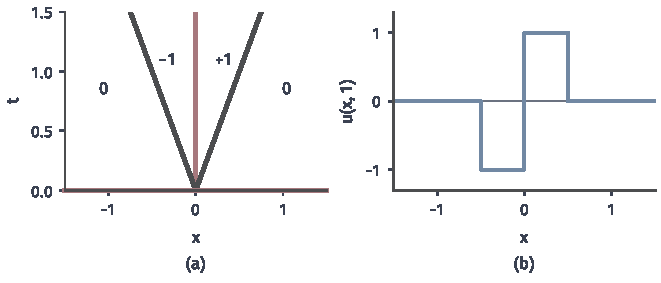
\includegraphics[width=112mm]{figures/06-differential-equations/02-partial-differential-equations/matplotlib/cons-zero-data/figure.pdf}
  \caption{零初值的非零弱解，$b=1$。(a)$(x,t)$平面，数字是各区域的值，红色粗线$x=0$是向上的跳跃，两条深灰粗线是向下的跳跃。(b)$t=1$的形状，正负两块面积相互抵消。}
  \label{fig:cons-zero-data}
\end{BookInlineFigure}

\paragraph{特征线必须汇入间断}
看特征线在间断两侧的走向就能分出好坏。先看图~\ref{fig:cons-lax-in-out}(a)，其中$u_-=1$、$u_+=0$，$s=1/2$。左侧特征线的速度$1$大于$s$，从后面追上间断；右侧特征线的速度$0$小于$s$，被间断追上。两侧的特征线都汇入间断，间断两侧的状态都由更早的初值决定。

(b)中$u_-=0$、$u_+=1$，$s$同样是$1/2$，方向却反了：左侧速度$0$小于$s$，右侧速度$1$大于$s$，特征线都从间断上离开。这些特征线沿途携带的值并不来自初值，只能在间断线上凭空产生。这就是前面的解不唯一的根源：既然这些值无从确定，它们就可以任意选取。

\begin{BookInlineFigure}
  \centering
  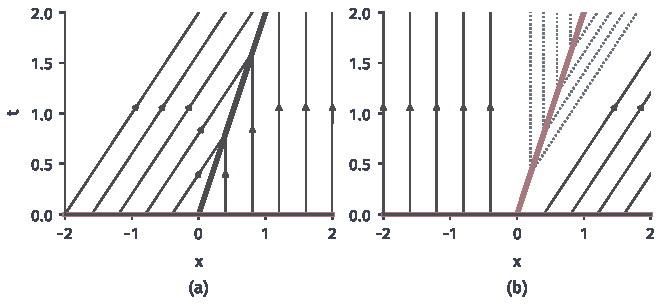
\includegraphics[width=112mm]{figures/06-differential-equations/02-partial-differential-equations/matplotlib/cons-lax-in-out/figure.pdf}
  \caption{两种间断两侧的特征线，$s$都是$1/2$，箭头指向时间增大的方向。(a)$u_-=1$、$u_+=0$（深灰粗线），两侧特征线都汇入。(b)$u_-=0$、$u_+=1$（红色粗线），点线表示从间断上发出的特征线，初值决定不了它们的取值。}
  \label{fig:cons-lax-in-out}
\end{BookInlineFigure}

把这一观察写成条件，就是\term{Lax熵条件}（Lax entropy condition）：
\begin{equation}
  F'(u_-)>s>F'(u_+).
  \label{eq:cons-lax}
\end{equation}

满足这一条件的间断称为\term{激波}（shock wave）。$F$严格凸时条件有更简单的形式。此时$F'$严格递增，$s$是$F'$在$u_-$与$u_+$之间的平均，严格落在两端值之间。所以当$u_-\neq u_+$时，式~\eqref{eq:cons-lax}等价于$F'(u_-)>F'(u_+)$，也就是$u_->u_+$。

对Burgers方程这句话是说，只有向下的跳跃才允许存在。检验前面的例子：$(u_-,u_+)=(1,0)$满足$1>1/2>0$；$(0,1)$要求$0>1/2>1$，不成立。凹的车流通量则相反，要求$u_-<u_+$：前方密度大、后方密度小，正是车辆追上堵车队尾的情形。例如$u_-=0.2$、$u_+=0.8$时
\[
  s=\frac{0.16-0.16}{0.6}=0,\qquad F'(0.2)=0.6>0>-0.6=F'(0.8),
\]
队尾静止不动，两侧的扰动都汇向队尾。

式~\eqref{eq:cons-lax}只适用于分段光滑的解和凸通量。要对一般的有界解下定义，得从这条规则的来源说起。

\paragraph{消失黏性}
真实的流体和车流都有一点扩散：司机会根据前方密度提前调整。在方程里加上小的黏性项，
\begin{equation}
  \partial_tu^{\nu}+\partial_xF(u^{\nu})=\nu\,\partial_{xx}u^{\nu},\qquad \nu>0.
  \label{eq:cons-viscous}
\end{equation}
式~\eqref{eq:cons-viscous}是抛物型方程，第~\ref{chap:diffusion-equations}章的抹平作用使它的解保持光滑，也没有多解的问题。合理的弱解应该是$\nu\to0$时的极限。这种通过\term{消失黏性}（vanishing viscosity）挑选解的做法，可以在Burgers方程上算到底。

寻找行波解$u^{\nu}=U(\xi)$，$\xi=x-st$，$U(\pm\infty)=u_\pm$。代入Burgers方程，得到
\[
  -sU'+UU'=\nu U'' .
\]

对$\xi$积分一次，积分常数记为$C$：
\[
  -sU+\frac{U^2}{2}=\nu U'+C .
\]

令$\xi\to\pm\infty$，$U'\to0$，两端各给一个等式：
\[
  C=-su_-+\frac{u_-^2}{2}=-su_++\frac{u_+^2}{2}.
\]
当$u_-\neq u_+$时，消去$C$得到$s=(u_-+u_+)/2$，Rankine--Hugoniot条件自动出现。把$s$与$C=-u_-u_+/2$代回，一阶方程化为
\begin{equation}
  \nu U'=\frac12(U-u_-)(U-u_+).
  \label{eq:cons-viscous-profile}
\end{equation}

右端在$U$介于$u_-$与$u_+$之间时为负，所以$U$只能沿$\xi$递减。从$\xi=-\infty$的$u_-$走到$\xi=+\infty$的$u_+$，就必须$u_->u_+$。向上的跳跃没有黏性剖面，向下的跳跃才有。解出这个分离变量方程，得到
\begin{equation}
  U(\xi)=\frac{u_-+u_+}{2}-\frac{u_--u_+}{2}\tanh\frac{(u_--u_+)\,\xi}{4\nu}.
  \label{eq:cons-viscous-tanh}
\end{equation}

过渡层的宽度约为$4\nu/(u_--u_+)$，$\nu\to0$时剖面收缩成跳跃，见图~\ref{fig:cons-viscous-profile}。这是黏性对向下跳跃的解释：很薄的一层里，压缩和扩散互相平衡。

\begin{BookInlineFigure}
  \centering
  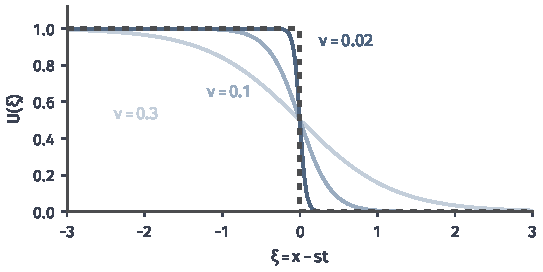
\includegraphics[width=92mm]{figures/06-differential-equations/02-partial-differential-equations/matplotlib/cons-viscous-profile/figure.pdf}
  \caption{Burgers方程的黏性行波~\eqref{eq:cons-viscous-tanh}，$u_-=1$、$u_+=0$。蓝色由浅到深是$\nu=0.3,0.1,0.02$，深灰点线是$\nu\to0$的极限跳跃。}
  \label{fig:cons-viscous-profile}
\end{BookInlineFigure}

向上的阶跃又如何？图~\ref{fig:cons-viscous-fan}把式~\eqref{eq:cons-viscous}从阶跃初值$0$、$1$开始算到$t=1$。数值解没有靠近跳跃$u^{\mathrm{j}}$，而是贴向连续的扇形$u^{\mathrm{f}}$。在弱解族~\eqref{eq:cons-weak-family}中，黏性选中的是$\alpha=0$。

\begin{BookInlineFigure}
  \centering
  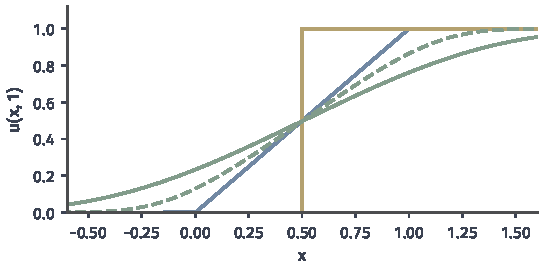
\includegraphics[width=92mm]{figures/06-differential-equations/02-partial-differential-equations/matplotlib/cons-viscous-fan/figure.pdf}
  \caption{阶跃初值$0$、$1$的黏性解在$t=1$的形状，由守恒的显式差分格式算出。绿色实线和虚线是$\nu=0.1$和$\nu=0.02$，蓝线是扇形解$u^{\mathrm{f}}$，黄线是跳跃解$u^{\mathrm{j}}$。$\nu$减小时数值解靠向蓝线。}
  \label{fig:cons-viscous-fan}
\end{BookInlineFigure}

\paragraph{熵不等式}
小黏性留下了什么可以在极限中保存的信息？取任意$C^2$凸函数$\eta$，再取$q$使$q'=\eta'F'$。这样的一对$(\eta,q)$称为\term{熵对}（entropy pair），$\eta$是熵，$q$是\term{熵通量}（entropy flux）。方程~\eqref{eq:cons-viscous}乘以$\eta'(u^{\nu})$，用链式法则整理：
\[
  \partial_t\eta(u^{\nu})+\partial_xq(u^{\nu})
  =\nu\,\partial_{xx}\eta(u^{\nu})-\nu\,\eta''(u^{\nu})\,(\partial_xu^{\nu})^2 .
\]

最后一项因为$\eta$凸而非正，它记录了扩散带来的耗散，正是这一项在极限中留下了方向。乘以$\varphi\geq0$并积分，分部积分后丢掉非负的耗散项，得到
\[
  \iint\bigl(\eta(u^{\nu})\,\partial_t\varphi+q(u^{\nu})\,\partial_x\varphi\bigr)\,\mathrm{d}x\,\mathrm{d}t
  \geq-\nu\iint\eta(u^{\nu})\,\partial_{xx}\varphi\,\mathrm{d}x\,\mathrm{d}t .
\]
假定$u^{\nu}$一致有界且几乎处处收敛，令$\nu\to0$，右端趋于零，留下一个不含$\nu$的不等式。这段推导只说明了不等式的来源，下面把它取作定义。

\begin{definition}[熵解]
\label{def:cons-entropy-solution}
设$F\in C^1(\mathbb{R})$，$u_0\in L^{\infty}(\mathbb{R})$。函数$u\in L^{\infty}(\mathbb{R}\times(0,\infty))$称为问题~\eqref{eq:cons-law}、\eqref{eq:cons-initial}的\term{熵解}（entropy solution），若对每个$C^2$凸函数$\eta$、满足$q'=\eta'F'$的$q$，以及每个非负的$\varphi\in C_c^{\infty}(\mathbb{R}\times(0,\infty))$，
\begin{equation}
  \int_0^{\infty}\!\!\int_{\mathbb{R}}\bigl(\eta(u)\,\partial_t\varphi+q(u)\,\partial_x\varphi\bigr)\,\mathrm{d}x\,\mathrm{d}t\geq0 ,
  \label{eq:cons-entropy-ineq}
\end{equation}
并且对每个$R>0$，初值在下述意义下取到：
\begin{equation}
  \operatorname*{ess\,lim}_{t\downarrow0}\int_{-R}^{R}\lvert u(x,t)-u_0(x)\rvert\,\mathrm{d}x=0 .
  \label{eq:cons-entropy-initial}
\end{equation}
\end{definition}

不等式~\eqref{eq:cons-entropy-ineq}是$\partial_t\eta(u)+\partial_xq(u)\leq0$的弱形式。取$\eta(u)=u$、$q=F$和$\eta(u)=-u$、$q=-F$，两者都是凸的，两个不等式合起来给出等式，再结合式~\eqref{eq:cons-entropy-initial}，熵解一定是弱解。$C^1$解由链式法则使式~\eqref{eq:cons-entropy-ineq}取等号，所以经典解也是熵解。

“熵”的名字来自气体动力学，那里的物理熵经过激波只增不减；数学上取凸函数，符号相反，所以$\eta$的总量只减不增。凸性的作用是把扩散耗散的符号固定下来。可以把$\eta(u)$想成一种能量：光滑时它和$u$一样守恒，只在间断处被消耗。

\paragraph{跨间断的熵不等式}
分段光滑的解要满足什么条件？重复定理~\ref{thm:cons-rh}的散度计算，把$(u,F(u))$换成$(\eta(u),q(u))$。在间断线两侧光滑部分的贡献为零，只留下线积分，于是式~\eqref{eq:cons-entropy-ineq}等价于
\begin{equation}
  q(u_+)-q(u_-)-s\bigl(\eta(u_+)-\eta(u_-)\bigr)\leq0 .
  \label{eq:cons-jump-entropy}
\end{equation}

左端是单位时间内在间断上产生的熵。取Burgers方程、$\eta=u^2/2$、$q=u^3/3$，并用$s=(u_-+u_+)/2$。记$\Delta=u_+-u_-$，直接展开：
\[
  \begin{aligned}
    \frac{u_+^3-u_-^3}{3}-\frac{(u_-+u_+)(u_+^2-u_-^2)}{4}
    &=\Delta\,\frac{4(u_+^2+u_+u_-+u_-^2)-3(u_-+u_+)^2}{12}\\
    &=\frac{\Delta^3}{12}.
  \end{aligned}
\]

所以间断上的能量变化率恰好是
\begin{equation}
  \frac{(u_+-u_-)^3}{12},
  \label{eq:cons-energy-rate}
\end{equation}
它非正当且仅当$u_+\leq u_-$。向下的跳跃消耗能量，向上的跳跃产生能量。

用斜坡解~\eqref{eq:cons-ramp-shock}核对一下。$t\geq1$时，在包含间断的大区间上，$\int u^2/2\,\mathrm{d}x$的增长率是$1/4$，因为$u=1$的区域以速度$1/2$延伸，每单位长度带能量$1/2$。左端流入能量的速率是$q(1)=1/3$。两者相差
\[
  \frac13-\frac14=\frac{1}{12},
\]
正是式~\eqref{eq:cons-energy-rate}在$(u_-,u_+)=(1,0)$时给出的耗散率。

零初值的解~\eqref{eq:cons-zero-data}同样可以算账。中间的跳跃$-b\to b$产生能量$(2b)^3/12=2b^3/3$，两侧的跳跃各消耗$b^3/12$，净产生率为$b^3/2$，这正是总能量$b^3t/2$的增长率。这个解违反熵不等式，错就错在中间那条向上的跳跃。

图~\ref{fig:cons-energy-decay}显示贯穿例子的情况：$T^{*}$之前能量守恒，激波形成之后能量按式~\eqref{eq:cons-energy-rate}减少，而总量一直不变。这是守恒律与熵的区别：总量是真正守恒的量，熵只有在光滑时才守恒。

\begin{BookInlineFigure}
  \centering
  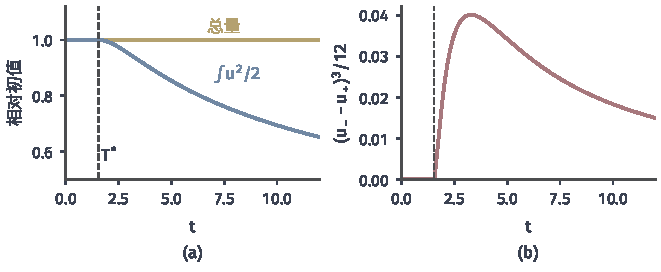
\includegraphics[width=112mm]{figures/06-differential-equations/02-partial-differential-equations/matplotlib/cons-energy-decay/figure.pdf}
  \caption{初值~\eqref{eq:cons-bump}的总量与能量。(a)黄线是总量$\int u\,\mathrm{d}x$相对初值的比，蓝线是能量$\int u^2/2\,\mathrm{d}x$相对初值的比，虚线是$T^{*}$。(b)激波上的耗散率$(u_--u_+)^3/12$，$T^{*}$之前为零。}
  \label{fig:cons-energy-decay}
\end{BookInlineFigure}

\paragraph{一族就够：Kruzhkov熵}
定义要求对所有凸熵成立，用起来需要一族足够简单的代表。对每个$k\in\mathbb{R}$，令
\begin{equation}
  \eta_k(u)=\lvert u-k\rvert,\qquad q_k(u)=\operatorname{sgn}(u-k)\bigl(F(u)-F(k)\bigr),
  \label{eq:cons-kruzhkov-pair}
\end{equation}
这称为\term{Kruzhkov熵}（Kruzhkov entropy）。它不是$C^2$的，但下面的引理说明，只需检验这一族。

\begin{lemma}[Kruzhkov熵的充分性]
\label{lem:cons-kruzhkov}
设$F\in C^1$，$u$有界。式~\eqref{eq:cons-entropy-ineq}对所有$C^2$凸熵对成立，当且仅当对每个$k\in\mathbb{R}$和每个$\varphi\geq0$，
\begin{equation}
  \int_0^{\infty}\!\!\int_{\mathbb{R}}\bigl(\lvert u-k\rvert\,\partial_t\varphi+q_k(u)\,\partial_x\varphi\bigr)\,\mathrm{d}x\,\mathrm{d}t\geq0 .
  \label{eq:cons-kruzhkov}
\end{equation}
\end{lemma}

\begin{proof}
必要性：取$C^2$凸函数及与之配对的熵通量
\[
  \eta_\delta(u)=\sqrt{(u-k)^2+\delta^2}-\delta,\qquad
  q_\delta(u)=\int_k^u\eta_\delta'(w)F'(w)\,\mathrm{d}w .
\]
$\delta\to0$时，在有界集上$\eta_\delta\to\lvert u-k\rvert$，$q_\delta\to q_k$，且都是一致收敛，不等式取极限成立。

充分性：记$\lVert u\rVert_{L^\infty}\leq M$。对$C^2$凸函数$\eta$，在$[-M,M]$上有表示
\[
  \eta(u)=\alpha u+\beta+\frac12\int_{-M}^{M}\eta''(k)\,\lvert u-k\rvert\,\mathrm{d}k .
\]
这是因为两端的二阶导数都是$\eta''$，差是仿射函数。

对上式求导，得到
\[
  \eta'(u)=\alpha+\frac12\int_{-M}^{M}\eta''(k)\operatorname{sgn}(u-k)\,\mathrm{d}k .
\]

乘以$F'(u)$再积分，熵通量有对应的表示：
\[
  q(u)=\alpha F(u)+\beta'+\frac12\int_{-M}^{M}\eta''(k)\,q_k(u)\,\mathrm{d}k .
\]

取$k=M$和$k=-M$，式~\eqref{eq:cons-kruzhkov}中$\lvert u-k\rvert$分别是$M-u$和$u+M$，两个不等式合起来说明$u$满足式~\eqref{eq:cons-rh-weak}形式的等式，于是仿射部分的贡献为零。常数项$\beta,\beta'$积分后也为零。其余部分是式~\eqref{eq:cons-kruzhkov}按非负权重$\eta''(k)/2$对$k$的积分，所以非负。
\end{proof}

现在可以回答跨间断的问题：对一个满足跳跃条件的间断，熵条件到底要求什么。记$L(k)$是通量图像上连接两个状态的弦，
\begin{equation}
  L(k)=F(u_-)+s\,(k-u_-).
  \label{eq:cons-chord}
\end{equation}

\begin{theorem}[跨间断的熵判据]
\label{thm:cons-chord}
设$F\in C^1$，$u_-\neq u_+$，$s$由式~\eqref{eq:cons-shock-speed}给出。则式~\eqref{eq:cons-jump-entropy}对所有$C^2$凸熵对成立，当且仅当对$u_-$与$u_+$之间的每个$k$，
\begin{equation}
  \begin{cases}
    F(k)\leq L(k),&u_->u_+,\\
    F(k)\geq L(k),&u_-<u_+.
  \end{cases}
  \label{eq:cons-oleinik}
\end{equation}
特别地，$F$严格凸时，熵判据等价于$u_->u_+$，也等价于式~\eqref{eq:cons-lax}。
\end{theorem}

\begin{proof}
记$D(\eta,q)$是式~\eqref{eq:cons-jump-entropy}的左端。$D$关于$(\eta,q)$是线性的，由引理~\ref{lem:cons-kruzhkov}中的表示，只需计算$D_k=D(\eta_k,q_k)$。仿射部分贡献$\alpha(F(u_+)-F(u_-)-s(u_+-u_-))=0$，这用到了跳跃条件。

$k$不在$u_-$与$u_+$之间时，$\operatorname{sgn}(u-k)$在两个状态上相同，$D_k$是跳跃条件的一个倍数，等于零。

设$u_->k>u_+$。此时$\eta_k(u_-)=u_--k$，$\eta_k(u_+)=k-u_+$，相应的熵通量是$F(u_-)-F(k)$和$F(k)-F(u_+)$。代入得到
\[
  D_k=2F(k)-F(u_+)-F(u_-)-s\,(2k-u_+-u_-).
\]

由式~\eqref{eq:cons-chord}和跳跃条件$F(u_+)=F(u_-)+s(u_+-u_-)$，上式整理为
\[
  D_k=2\bigl(F(k)-L(k)\bigr).
\]
所以$D_k\leq0$当且仅当$F(k)\leq L(k)$。$u_-<k<u_+$时两个符号都反过来，$D_k=-2(F(k)-L(k))$，于是$D_k\leq0$当且仅当$F(k)\geq L(k)$。

必要性取$D_k\leq0$对$C^2$逼近的极限；充分性把$D_k\leq0$按非负权重$\eta''(k)/2$积分。

$F$严格凸时，弦严格在图像上方，$F(k)<L(k)$，第二种情形不可能，第一种情形总成立。
\end{proof}

式~\eqref{eq:cons-oleinik}称为\term{Oleinik条件}（Oleinik condition），图~\ref{fig:cons-oleinik-chord}是它的几何图景。它同时覆盖凸与非凸通量，比式~\eqref{eq:cons-lax}更一般：跳跃能否存在，取决于通量图像在两个状态之间落在弦的哪一边。用$k=1/2$检验$(u_-,u_+)=(1,0)$：$F(1/2)=1/8$，$L(1/2)=1/4$，$D_k=2(1/8-1/4)=-1/4\leq0$，熵不等式成立。

\begin{BookInlineFigure}
  \centering
  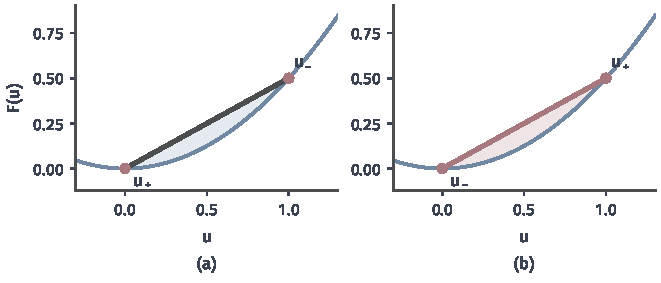
\includegraphics[width=112mm]{figures/06-differential-equations/02-partial-differential-equations/matplotlib/cons-oleinik-chord/figure.pdf}
  \caption{Oleinik条件，$F=u^2/2$（蓝）。两图的弦相同，红点是两个状态。(a)$u_->u_+$，要求图像在弦下方（浅蓝），成立。(b)$u_-<u_+$，要求图像在弦上方，凸函数的图像却在下方（浅红），不成立。}
  \label{fig:cons-oleinik-chord}
\end{BookInlineFigure}

消失黏性的说明到这里还只是形式推导。严格的结论是：$F\in C^1$、$u_0\in L^{\infty}$时，式~\eqref{eq:cons-viscous}的解在$\nu\to0$时在$L^1_{\mathrm{loc}}$中收敛到熵解。证明需要用到解的一致有界性、全变差估计和紧性论证，篇幅较长，读者可查阅Kruzhkov于1970年发表的原始论文或双曲守恒律的专著。这个定理说明熵条件的选择与物理上的小黏性是一致的。


\section{Riemann问题}
\label{sec:cons-riemann}

最简单的不连续初值是左右两个常状态：
\begin{equation}
  u_0(x)=\begin{cases}u_l,&x<0,\\u_r,&x>0.\end{cases}
  \label{eq:cons-riemann-data}
\end{equation}
这称为\term{Riemann问题}（Riemann problem）。守恒、特征线和熵条件在这里都能落实成手算。

有一条结构可以先用上。方程和初值在缩放$(x,t)\mapsto(\lambda x,\lambda t)$下不变，若解唯一（下一节证明），解就只依赖于比值$\xi=x/t$，形如$u=w(\xi)$。这样的解称为\term{自相似解}（self-similar solution）。在$(x,t)$平面上，它沿着从原点出发的每条射线取常值。

本节先设$F$严格凸。此时$F'$严格递增，按上一节的结论，$u_l>u_r$时阶跃本身是可接受的间断，$u_l<u_r$时不是。这两种情形分别对应两种完全不同的波。

\subsection{激波}
\label{subsec:cons-shock}

左状态大于右状态时，$F'(u_l)>F'(u_r)$，左边的特征线比右边的快，迎面相撞，只能产生间断。

\begin{theorem}[激波解]
\label{thm:cons-shock}
设$F\in C^1$严格凸，$u_l>u_r$。令
\begin{equation}
  s=\frac{F(u_l)-F(u_r)}{u_l-u_r},\qquad
  u(x,t)=\begin{cases}u_l,&x<st,\\u_r,&x>st.\end{cases}
  \label{eq:cons-shock-solution}
\end{equation}
则$u$是Riemann问题的熵解。
\end{theorem}

\begin{proof}
$u$分块为常数，满足方程。$s$由式~\eqref{eq:cons-shock-speed}给出，跳跃条件成立。由定理~\ref{thm:cons-chord}，$u_->u_+$时式~\eqref{eq:cons-jump-entropy}对所有凸熵对成立，所以式~\eqref{eq:cons-entropy-ineq}成立。最后，$u$与初值只在宽度为$\lvert s\rvert t$的区间上不同，差不超过$u_l-u_r$，式~\eqref{eq:cons-entropy-initial}成立。
\end{proof}

波速由两侧状态共同决定，任何一侧单独都定不下来。表~\ref{tab:cons-shock-examples}列出几组数据。Burgers方程的波速是两侧状态的算术平均，这是平方通量的特殊之处；最后一行的通量$F=u^4/4$严格凸，波速$15/4$并不等于两侧传播速度的平均$9/2$。每一行都满足$F'(u_l)>s>F'(u_r)$。

\begin{BookInlineTable}
  \centering
  \caption{激波速度的手算。前四行是Burgers方程，第五行$F=u^4/4$，每一行都验证了$F'(u_l)>s>F'(u_r)$。}
  \label{tab:cons-shock-examples}
  \begin{tabular}{cccccc}
    \toprule
    通量 & $u_l$ & $u_r$ & $s$ & $F'(u_l)$ & $F'(u_r)$\\
    \midrule
    $u^2/2$ & $2$ & $0$ & $1$ & $2$ & $0$\\
    $u^2/2$ & $2$ & $1$ & $3/2$ & $2$ & $1$\\
    $u^2/2$ & $1$ & $-1$ & $0$ & $1$ & $-1$\\
    $u^2/2$ & $0$ & $-2$ & $-1$ & $0$ & $-2$\\
    $u^4/4$ & $2$ & $1$ & $15/4$ & $8$ & $1$\\
    \bottomrule
  \end{tabular}
\end{BookInlineTable}

取第一行$u_l=2$、$u_r=0$，$s=1$，解在图~\ref{fig:cons-riemann-shock}中。用矩形$[-1,3]\times[0,1]$核对收支：初始总量是$2\cdot1=2$，$t=1$时$x<1$的部分长度为$2$，总量是$4$，左端流入$F(2)\cdot1=2$，右端流出$0$，正好$2+2=4$。第三行的$s=0$说明波速可以为零，第四行的$s=-1$说明激波可以向左传播。

\begin{BookInlineFigure}
  \centering
  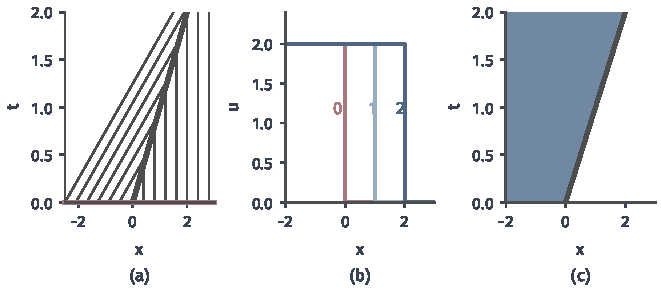
\includegraphics[width=112mm]{figures/06-differential-equations/02-partial-differential-equations/matplotlib/cons-riemann-shock/figure.pdf}
  \caption{Burgers方程的Riemann问题$u_l=2$、$u_r=0$，$s=1$。(a)特征线（细线）从两侧汇入激波（深灰粗线）。(b)红线是$t=0$，蓝色由浅到深是$t=1,2$。(c)时空平面上的场，颜色越深值越大。}
  \label{fig:cons-riemann-shock}
\end{BookInlineFigure}

\subsection{稀疏波}
\label{subsec:cons-rarefaction}

左状态小于右状态时，$F'(u_l)<F'(u_r)$，左边的特征线比右边的慢，它们彼此分开。图~\ref{fig:cons-riemann-fan}(a)中，浅红的楔形区域没有任何特征线到达，式~\eqref{eq:cons-implicit}在那里什么也没有告诉我们。阶跃本身还是可以当作弱解，但它在上一节已经被熵条件排除，楔形必须用别的东西填满。

\begin{BookInlineFigure}
  \centering
  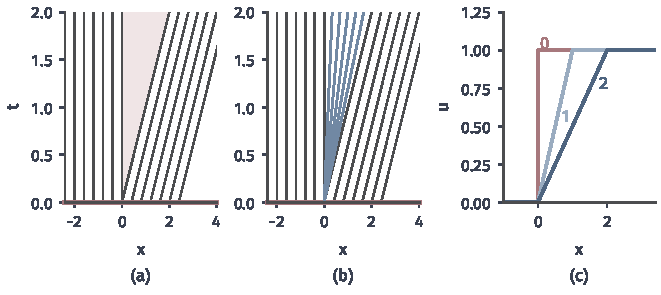
\includegraphics[width=112mm]{figures/06-differential-equations/02-partial-differential-equations/matplotlib/cons-riemann-fan/figure.pdf}
  \caption{Burgers方程的Riemann问题$u_l=0$、$u_r=1$。(a)只画初始线出发的特征线，留下一片浅红的空白楔形。(b)从原点发出的扇形特征线（蓝）填满楔形。(c)红线是$t=0$，蓝色由浅到深是$t=1,2$，斜坡的宽度随时间线性增长。}
  \label{fig:cons-riemann-fan}
\end{BookInlineFigure}

用自相似的形式求解。把$u=w(\xi)$，$\xi=x/t$代入式~\eqref{eq:cons-quasilinear}，$\partial_tu=-\xi w'/t$，$\partial_xu=w'/t$，得到
\[
  \frac{w'(\xi)}{t}\bigl(F'(w(\xi))-\xi\bigr)=0 .
\]

所以每一点要么$w'=0$（常状态），要么$F'(w(\xi))=\xi$。后者说明，填补楔形的解满足$F'(w)=\xi$，也就是把初始间断点看成同时发出所有速度的特征线的源头：每条射线$x=\xi t$就是一条特征线，速度恰好是$\xi$。这样得到的解称为\term{稀疏波}（rarefaction wave）。

\begin{theorem}[稀疏波解]
\label{thm:cons-rarefaction}
设$F\in C^2$，在$[u_l,u_r]$上$F''>0$，$u_l<u_r$。令
\begin{equation}
  u(x,t)=\begin{cases}
    u_l,&x\leq F'(u_l)\,t,\\
    (F')^{-1}(x/t),&F'(u_l)\,t<x<F'(u_r)\,t,\\
    u_r,&x\geq F'(u_r)\,t.
  \end{cases}
  \label{eq:cons-rarefaction}
\end{equation}
则$u$连续（$t>0$），并且是Riemann问题的熵解。
\end{theorem}

\begin{proof}
$F'$在$[u_l,u_r]$上严格递增，逆函数$(F')^{-1}$是$C^1$的，所以式~\eqref{eq:cons-rarefaction}有定义。在扇形边界上它的值分别是$u_l$、$u_r$，$u$在$t>0$连续。

在扇形内，记$w=(F')^{-1}$，有$F''(w)\,w'=1$，于是
\[
  \partial_tu+F'(u)\,\partial_xu
  =-\frac{x}{t^2}w'+\frac{x}{t}\cdot\frac{w'}{t}=0 .
\]

$u$在各块上是$C^1$的，满足方程，由链式法则，每一块上$\partial_t\eta(u)+\partial_xq(u)=0$。两条接缝上$u$连续，式~\eqref{eq:cons-jump-entropy}的左端为零。所以式~\eqref{eq:cons-entropy-ineq}取等号成立。最后，$u$只在宽度不超过$\max\lvert F'\rvert\,t$的区间上与初值不同，差不超过$u_r-u_l$，式~\eqref{eq:cons-entropy-initial}成立。
\end{proof}

Burgers方程$F'(u)=u$，$(F')^{-1}$是恒等映射，取$(u_l,u_r)=(0,1)$，得到
\begin{equation}
  u(x,t)=\frac{x}{t},\qquad 0<x<t,
  \label{eq:cons-burgers-fan}
\end{equation}
这正是前面的$u^{\mathrm{f}}$。$F=u^4/4$、$(u_l,u_r)=(1,2)$时，$F'(u)=u^3$，扇形占据$1<x/t<8$，解是$u=(x/t)^{1/3}$。扇形边缘的速度由两侧状态各自决定，而不是取什么平均：左边缘$F'(u_l)$，右边缘$F'(u_r)$。

\paragraph{扇形是连续依赖的结果}
稀疏波可以由经典解的极限得到。把阶跃$0$、$1$替换成宽度为$\varepsilon$的斜坡，$u_0=x/\varepsilon$（$0\leq x\leq\varepsilon$）。这个初值单调不减，定理~\ref{thm:cons-lifespan}说解永远不会失去光滑性。由特征线$x=x_0+(x_0/\varepsilon)t$反解$x_0=\varepsilon x/(\varepsilon+t)$，得到
\begin{equation}
  u^{\varepsilon}(x,t)=\frac{x}{\varepsilon+t},\qquad 0\leq x\leq\varepsilon+t .
  \label{eq:cons-smoothed-step}
\end{equation}

令$\varepsilon\to0$，式~\eqref{eq:cons-smoothed-step}收敛到扇形~\eqref{eq:cons-burgers-fan}，如图~\ref{fig:cons-smoothed-step}。所以向上的阶跃是一个不稳定的状态：无论把初值磨得多么轻微，解都立刻选择扇形。跳跃解$u^{\mathrm{j}}$经不起这样的扰动，这是排除它的又一条理由。

\begin{BookInlineFigure}
  \centering
  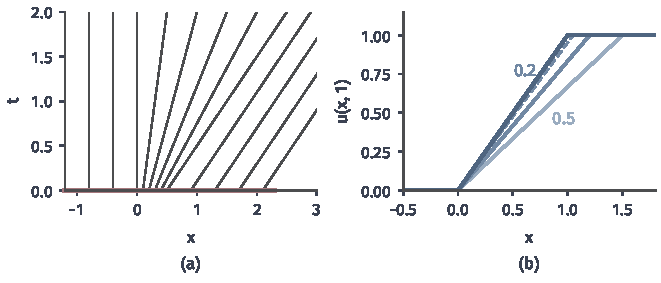
\includegraphics[width=112mm]{figures/06-differential-equations/02-partial-differential-equations/matplotlib/cons-smoothed-step/figure.pdf}
  \caption{磨光的阶跃。(a)$\varepsilon=0.5$的特征线，从斜坡出发的特征线彼此张开，永不相交。(b)解~\eqref{eq:cons-smoothed-step}在$t=1$的形状，蓝色由浅到深是$\varepsilon=0.5,0.2$，虚线是$\varepsilon=0.05$，最深的蓝线是扇形。}
  \label{fig:cons-smoothed-step}
\end{BookInlineFigure}

表~\ref{tab:cons-wave-comparison}把三种候选放在一起对比。

\begin{BookInlineTable}
  \centering
  \caption{严格凸通量下的三种波。}
  \label{tab:cons-wave-comparison}
  \begin{tabular}{cccc}
    \toprule
    & 激波 & 稀疏波 & 扩张间断\\
    \midrule
    状态 & $u_l>u_r$ & $u_l<u_r$ & $u_l<u_r$\\
    连续性 & 跳跃 & 连续 & 跳跃\\
    特征线 & 汇入 & 张开并填满 & 从间断发出\\
    能量（Burgers） & 减少 & 守恒 & 增加\\
    熵条件 & 满足 & 满足 & 违反\\
    \bottomrule
  \end{tabular}
\end{BookInlineTable}

\paragraph{波的相遇：方波}
Riemann解可以拼起来，用来算一般的初值。取Burgers方程和方波
\[
  u_0(x)=\begin{cases}1,&0<x<1,\\0,&\text{其他}.\end{cases}
\]

$x=0$处是向上的阶跃，产生扇形$u=x/t$；$x=1$处是向下的阶跃，产生激波，速度$1/2$。所以$t\leq2$时
\[
  u(x,t)=\begin{cases}x/t,&0<x<t,\\1,&t<x<1+t/2,\\0,&\text{其他}.\end{cases}
\]

扇形的右边缘$x=t$追赶激波$x=1+t/2$，相遇于$t=2$、$x=2$。此后激波左侧的状态不再是常数，而是扇形的值$\gamma/t$，右侧仍是$0$。由式~\eqref{eq:cons-burgers-speed}，激波位置$\gamma(t)$满足
\[
  \gamma'(t)=\frac{\gamma(t)}{2t},\qquad \gamma(2)=2 .
\]

分离变量解得$\gamma(t)=\sqrt{2t}$。于是$t\geq2$时的解是
\begin{equation}
  u(x,t)=\begin{cases}x/t,&0<x<\sqrt{2t},\\0,&\text{其他}.\end{cases}
  \label{eq:cons-box-late}
\end{equation}

波形成为一个三角形，高度$\gamma/t=\sqrt{2/t}$按$t^{-1/2}$衰减，底宽$\sqrt{2t}$按$t^{1/2}$增长。面积是
\[
  \frac12\cdot\sqrt{2t}\cdot\sqrt{\frac2t}=1 ,
\]
与初值的总量一致。图~\ref{fig:cons-box-interaction}展示了这个过程。

\begin{BookInlineFigure}
  \centering
  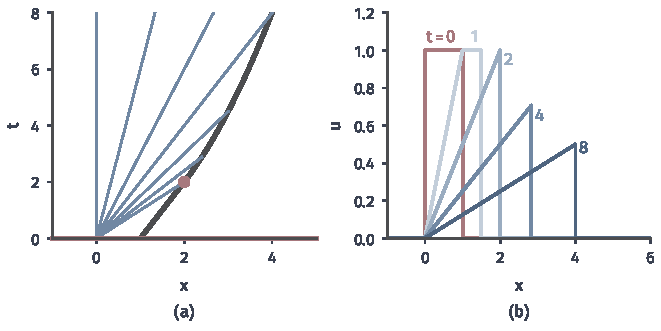
\includegraphics[width=112mm]{figures/06-differential-equations/02-partial-differential-equations/matplotlib/cons-box-interaction/figure.pdf}
  \caption{方波的演化。(a)蓝线是从原点发出的扇形特征线，深灰粗线是激波，红点$(2,2)$是扇形右边缘追上激波的位置，此后激波沿$x=\sqrt{2t}$弯曲。(b)红线是$t=0$，蓝色由浅到深是$t=1,2,4,8$，方波先变成梯形，再变成衰减的三角形。}
  \label{fig:cons-box-interaction}
\end{BookInlineFigure}

\paragraph{更一般的通量}
通量不凸时，单一的激波或扇形可能都不行，解由两者复合而成。规律是：$u_l>u_r$时取$F$在$[u_r,u_l]$上的上凹包络，$u_l<u_r$时取下凸包络；包络的直线段对应间断，严格弯曲的部分对应扇形。这一构造的完整证明要逐段验证Oleinik条件，较为繁琐，读者可查阅双曲守恒律的专著。下面验证一个具体的例子。

取$F(u)=u^3/3$，$(u_l,u_r)=(1,-1)$。$F$在$u<0$时凹，$u>0$时凸。从$(1,1/3)$作切线，切$F$的图像于$a<0$，条件是切线斜率等于弦斜率：
\[
  a^2=\frac{1/3-a^3/3}{1-a}=\frac{1+a+a^2}{3}.
\]

整理得$2a^2-a-1=0$，舍去$a=1$，取$a=-1/2$。于是解由三段组成：从$1$跳到$-1/2$的激波，速度$s=a^2=1/4$；然后是由$w^2=\xi$定出的扇形，$w=-\sqrt{\xi}$，$1/4<\xi<1$；最后是常状态$-1$。

检验激波部分。由式~\eqref{eq:cons-chord}，弦是$L(k)=1/3+(k-1)/4$，于是
\[
  F(k)-L(k)=\frac{4k^3-3k-1}{12}=\frac{(k-1)(2k+1)^2}{12}.
\]
在$k\in[-1/2,1]$上这个量非正，式~\eqref{eq:cons-oleinik}成立。切点$k=-1/2$处恰好为零，这正是激波与扇形相接的位置。

图~\ref{fig:cons-cubic-compound}把这个解和一个迎风差分格式的数值解画在一起，两者吻合。这种复合波说明，严格凸通量下的二分法不能照搬到一般通量。

\begin{BookInlineFigure}
  \centering
  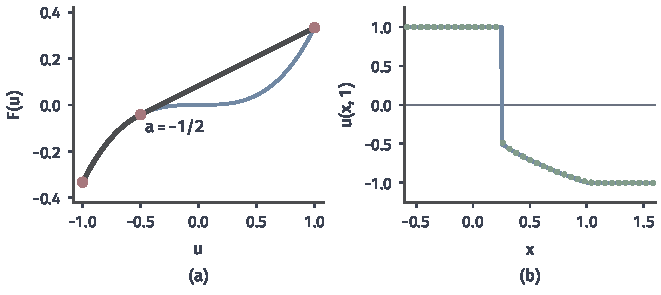
\includegraphics[width=112mm]{figures/06-differential-equations/02-partial-differential-equations/matplotlib/cons-cubic-compound/figure.pdf}
  \caption{非凸通量$F=u^3/3$的Riemann问题$u_l=1$、$u_r=-1$。(a)蓝线是$F$，深灰粗线是上凹包络，红点是端点和切点$a=-1/2$。(b)蓝线是$t=1$的精确解（激波接扇形），绿点是空间步长$2\times10^{-3}$的迎风格式的数值解。}
  \label{fig:cons-cubic-compound}
\end{BookInlineFigure}


\section{唯一性与稳定性}
\label{sec:cons-uniqueness}

熵条件排除了前面所有的反例，但这并不等于只剩下一个解。怎样证明同一初值的熵解只有一个？办法是比较两个熵解：证明它们的积分距离不会随时间增大。

\paragraph{距离为什么不增}
先看一个算得出的例子。比较斜坡初值~\eqref{eq:cons-ramp}的解$u$和阶跃初值的解$v$，阶跃位于$x=1/2$，左$1$右$0$。$v$是激波解，位置$x=(1+t)/2$。$u$在$t<1$时由式~\eqref{eq:cons-ramp-solution}给出，$t\geq1$时由式~\eqref{eq:cons-ramp-shock}给出。

$t<1$时，两个解只在区间$(t,1)$上不同。在激波位置$x=(1+t)/2$处，$u$的值是$1/2$，所以差的图像是两个全等的三角形，底为$(1-t)/2$，高为$1/2$。于是
\begin{equation}
  \lVert u(\cdot,t)-v(\cdot,t)\rVert_1=\frac{1-t}{4},\qquad 0\leq t\leq1.
  \label{eq:cons-merge-distance}
\end{equation}

$t=1$时距离为零，此后两个解完全相同，见图~\ref{fig:cons-merge-l1}。距离在减小，而且激波吞掉了两个初值之间的差别。

\begin{BookInlineFigure}
  \centering
  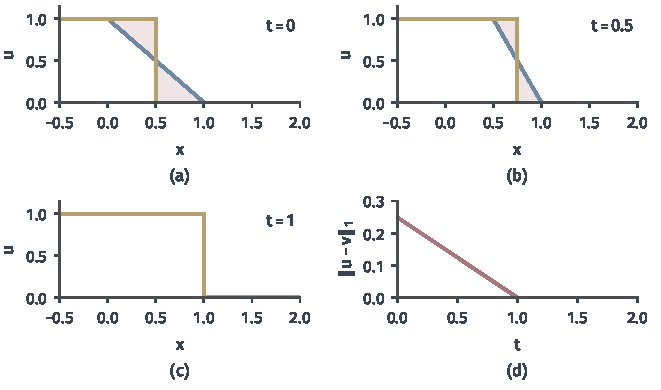
\includegraphics[width=112mm]{figures/06-differential-equations/02-partial-differential-equations/matplotlib/cons-merge-l1/figure.pdf}
  \caption{两个熵解的距离。蓝线是斜坡初值的解，黄线是阶跃初值的解，浅红区域的面积是两者的$L^1$距离。(a)$t=0$。(b)$t=0.5$。(c)$t=1$，两个解重合。(d)距离随时间的变化，$t\leq1$时为$(1-t)/4$，此后为零。}
  \label{fig:cons-merge-l1}
\end{BookInlineFigure}

\paragraph{收缩定理}
一般情形的结论如下。式中的常数$L$是系统中最大的传播速度，它决定了外部区域的影响能传多快。

\begin{theorem}[局部$L^1$收缩]
\label{thm:cons-contraction}
设$F\in C^1(\mathbb{R})$，$u,v$是初值$u_0,v_0\in L^{\infty}(\mathbb{R})$的两个熵解。取$M$使$\lvert u\rvert,\lvert v\rvert\leq M$几乎处处成立，令$L=\max_{\lvert w\rvert\leq M}\lvert F'(w)\rvert$。则对每个$R>0$和几乎处处的$T>0$，
\begin{equation}
  \int_{-R}^{R}\lvert u(x,T)-v(x,T)\rvert\,\mathrm{d}x
  \leq\int_{-R-LT}^{R+LT}\lvert u_0(x)-v_0(x)\rvert\,\mathrm{d}x .
  \label{eq:cons-local-contraction}
\end{equation}
\end{theorem}

图~\ref{fig:cons-cone}是这个不等式的几何含义。$t=T$时区间$[-R,R]$上的差，只由底边$[-R-LT,R+LT]$上的初值差决定，侧边以速度$L$向内收缩。间断可以穿过这个梯形，账依然成立。

\begin{BookInlineFigure}
  \centering
  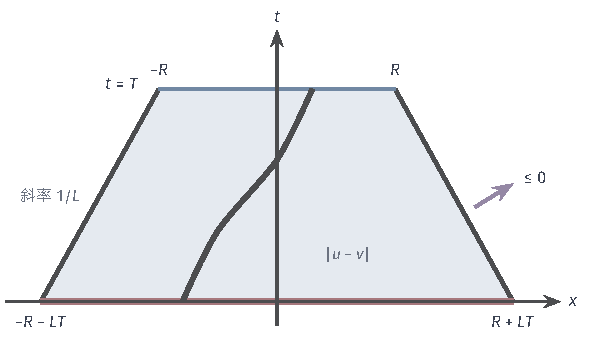
\includegraphics[width=99.8mm]{figures/06-differential-equations/02-partial-differential-equations/tikz/cons-cone/figure.pdf}
  \caption{依赖域梯形。底边（红）是初值差的积分范围，顶边（蓝）是$t=T$时的积分范围，两条侧边（深灰）的速度为$L$。紫色箭头表示穿过侧边的净流量不为正，即差不会从侧边流入。梯形内的深灰曲线是一条可能的间断线。}
  \label{fig:cons-cone}
\end{BookInlineFigure}

证明的难处在于$u$和$v$都不光滑，不能直接相减再求导。若是光滑解，$w=u-v$满足线性输运方程，$\lvert w\rvert$沿特征线的积分不增，结论立刻得到。Kruzhkov的办法是\term{变量加倍}（doubling of variables）：让$u$依赖$(x,t)$，$v$依赖独立的$(y,s)$，在式~\eqref{eq:cons-kruzhkov}中用一个解的值充当另一个解的常数$k$，最后用很窄的权重把$(y,s)$压回$(x,t)$，如图~\ref{fig:cons-doubling}。常数$k$在这里扮演的角色正是Kruzhkov熵的用处：熵不等式对每个$k$成立，$k$就可以取另一个解的值。

\begin{BookInlineFigure}
  \centering
  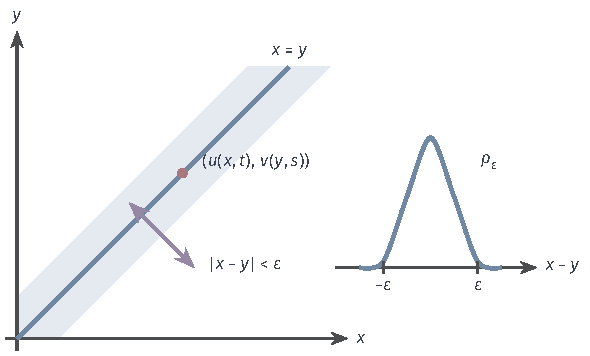
\includegraphics[width=99.9mm]{figures/06-differential-equations/02-partial-differential-equations/tikz/cons-doubling/figure.pdf}
  \caption{变量加倍的示意。左图是$(x,y)$平面（时间变量同理），两个解在两组独立变量上取值，浅蓝带是权重集中的区域，宽度约为$\varepsilon$。右图是横截面上的磨光核$\rho_\varepsilon$。令$\varepsilon\to0$，积分被压回对角线$x=y$。}
  \label{fig:cons-doubling}
\end{BookInlineFigure}

\begin{proof}
记$q(a,b)=\operatorname{sgn}(a-b)(F(a)-F(b))$。它关于$a,b$对称，并且当$\lvert a\rvert,\lvert b\rvert\leq M$时，
\[
  \lvert q(a,b)\rvert\leq L\,\lvert a-b\rvert .
\]

第一步，变量加倍。设$\phi(x,t,y,s)\geq0$是$(\mathbb{R}\times(0,\infty))^2$上的紧支光滑函数。固定$(y,s)$，在式~\eqref{eq:cons-kruzhkov}中对$u$取$k=v(y,s)$，再对$(y,s)$积分。类似地固定$(x,t)$，对$v$取$k=u(x,t)$，对$(x,t)$积分。两式相加，由$q$的对称性，
\[
  \iiiint\Bigl(\lvert u-v\rvert\,(\partial_t\phi+\partial_s\phi)
  +q(u,v)\,(\partial_x\phi+\partial_y\phi)\Bigr)\,\mathrm{d}x\,\mathrm{d}t\,\mathrm{d}y\,\mathrm{d}s\geq0 ,
\]
其中$u=u(x,t)$，$v=v(y,s)$。

第二步，选取测试函数。取非负$\psi\in C_c^{\infty}(\mathbb{R}\times(0,\infty))$和偶的标准磨光核$\rho_\varepsilon$，令
\[
  \phi=\psi\Bigl(\frac{x+y}{2},\frac{t+s}{2}\Bigr)\,
  \rho_\varepsilon\Bigl(\frac{x-y}{2}\Bigr)\,\rho_\varepsilon\Bigl(\frac{t-s}{2}\Bigr).
\]

求$\partial_t\phi+\partial_s\phi$时，$\rho_\varepsilon((t-s)/2)$的两项导数互相抵消，只剩$\psi$对时间的导数，空间变量同样。第一步的不等式化为
\[
  \iiiint\Bigl(\lvert u-v\rvert\,\partial_T\psi+q(u,v)\,\partial_X\psi\Bigr)\rho_\varepsilon\rho_\varepsilon\,\mathrm{d}x\,\mathrm{d}t\,\mathrm{d}y\,\mathrm{d}s\geq0 ,
\]
其中$\partial_T\psi,\partial_X\psi$在中点取值。

第三步，令$\varepsilon\to0$。作变量替换$X=(x+y)/2$，$\xi=(x-y)/2$，$T'=(t+s)/2$，$\tau=(t-s)/2$，Jacobian给出常数因子$4$。$\lvert a-b\rvert$与$q(a,b)$关于$a,b$是Lipschitz的，所以被积函数与其$\xi=\tau=0$时的值之差，被
\[
  C\bigl(\lvert u(X+\xi,T'+\tau)-u(X,T')\rvert+\lvert v(X-\xi,T'-\tau)-v(X,T')\rvert\bigr)
\]
控制。有界函数的平移在$L^1_{\mathrm{loc}}$中连续，这一项的积分在$\varepsilon\to0$时趋于零。于是对所有非负的$\psi$，
\begin{equation}
  \int_0^{\infty}\!\!\int_{\mathbb{R}}\Bigl(\lvert u-v\rvert\,\partial_t\psi+q(u,v)\,\partial_x\psi\Bigr)\,\mathrm{d}x\,\mathrm{d}t\geq0 .
  \label{eq:cons-kato}
\end{equation}

第四步，切出梯形。取$\delta\in(0,R)$和光滑不减函数$H_\delta$，$H_\delta(z)=0$（$z\leq-\delta$），$H_\delta(z)=1$（$z\geq0$）。取$\theta\in C_c^{\infty}(0,T)$，$\theta\geq0$，令
\[
  \psi(x,t)=\theta(t)\,\chi_\delta(x,t),\qquad
  \chi_\delta=1-H_\delta\bigl(\lvert x\rvert+L(t-T)-R\bigr).
\]
在$x=0$附近$H_\delta$的自变量小于$-\delta$，所以$\lvert x\rvert$的不光滑不影响$\psi$的光滑性。

记$H_\delta'$在上述自变量处取值，计算得
\[
  \partial_t\psi=\theta'\chi_\delta-\theta L H_\delta',\qquad
  \partial_x\psi=-\theta\operatorname{sgn}(x)H_\delta' .
\]

代入式~\eqref{eq:cons-kato}，整理后得到
\[
  \int_0^{T}\theta'(t)\int_{\mathbb{R}}\chi_\delta\,\lvert u-v\rvert\,\mathrm{d}x\,\mathrm{d}t
  \geq\iint\theta\,H_\delta'\,\bigl(L\,\lvert u-v\rvert+\operatorname{sgn}(x)\,q(u,v)\bigr)\,\mathrm{d}x\,\mathrm{d}t .
\]

$H_\delta'\geq0$，又由$\lvert q\rvert\leq L\lvert u-v\rvert$，右端非负。这一步是全部证明的关键：侧边的收缩速度$L$压过了流出的通量。

第五步，取极限。令$\delta\to0$，记
\[
  m(t)=\int_{\lvert x\rvert<R+L(T-t)}\lvert u(x,t)-v(x,t)\rvert\,\mathrm{d}x ,
\]
上面的不等式变成$\int_0^T\theta'(t)\,m(t)\,\mathrm{d}t\geq0$对所有非负的$\theta$成立。这说明$m$的弱导数非正，$m$几乎处处等于一个不增函数。

由式~\eqref{eq:cons-entropy-initial}，$t\downarrow0$时$m(t)$的本性极限是$\int_{\lvert x\rvert<R+LT}\lvert u_0-v_0\rvert\,\mathrm{d}x$。于是对几乎处处的$t\in(0,T)$，
\[
  \int_{\lvert x\rvert<R+L(T-t)}\lvert u-v\rvert\,\mathrm{d}x
  \leq\int_{\lvert x\rvert<R+LT}\lvert u_0-v_0\rvert\,\mathrm{d}x .
\]

令$R'=R+L(T-t)$，右端的半径就是$R'+Lt$，这正是要证的形式。让$(R,T)$取遍有理数，两端关于半径连续，所以结论对几乎处处的$t$和所有半径成立。
\end{proof}

证明中的两个地方用到了本章的条件。第一步的$k$可以取任意值，这需要Kruzhkov熵对所有$k$成立，只满足个别几个熵不够。第四步的$\lvert q\rvert\leq L\lvert u-v\rvert$需要$F$在解的取值范围内Lipschitz，这就是通量正则性与解有界的作用。

\paragraph{唯一性、收缩与比较}
把定理~\ref{thm:cons-contraction}用到不同的情形，就得到下面三条结论。比较原理需要把证明中的绝对值换成正部，做法很短，写在证明里。

\begin{theorem}[熵解的唯一性与稳定性]
\label{thm:cons-uniqueness}
在定理~\ref{thm:cons-contraction}的条件下：
\begin{enumerate}
  \item 若$u_0=v_0$几乎处处成立，则$u=v$几乎处处成立，即熵解唯一。
  \item 若$u_0-v_0\in L^1(\mathbb{R})$，则对几乎处处的$t>0$，
  \begin{equation}
    \lVert u(\cdot,t)-v(\cdot,t)\rVert_{1}\leq\lVert u_0-v_0\rVert_{1}.
    \label{eq:cons-l1-contraction}
  \end{equation}
  \item 若$u_0\leq v_0$几乎处处成立，则$u\leq v$几乎处处成立。特别地，$u$的值不超出$u_0$的本性下确界与本性上确界。
\end{enumerate}
\end{theorem}

\begin{proof}
第一条：式~\eqref{eq:cons-local-contraction}的右端为零。

第二条：在式~\eqref{eq:cons-local-contraction}中令$R\to\infty$。

第三条：$(u-k)^{+}$是凸函数，记$\operatorname{sgn}^{+}(z)$在$z>0$时为$1$，否则为$0$，与之配对的熵通量是$\operatorname{sgn}^{+}(u-k)(F(u)-F(k))$；$(k-v)^{+}$也是凸函数，熵通量是$\operatorname{sgn}^{+}(k-v)(F(k)-F(v))$。它们都是$C^2$凸熵的极限，所以各自满足式~\eqref{eq:cons-entropy-ineq}。

在变量加倍中，对$u$用前者并取$k=v(y,s)$，对$v$用后者并取$k=u(x,t)$，两式的被积函数相同，都是$(u-v)^{+}$和$\operatorname{sgn}^{+}(u-v)(F(u)-F(v))$。后者的绝对值同样不超过$L(u-v)^{+}$，所以第二步到第五步逐字照搬，得到
\[
  \int_{-R}^{R}(u-v)^{+}(x,T)\,\mathrm{d}x
  \leq\int_{-R-LT}^{R+LT}(u_0-v_0)^{+}\,\mathrm{d}x .
\]
$u_0\leq v_0$时右端为零，所以$u\leq v$。

常数是方程的熵解，取$v\equiv\operatorname*{ess\,sup}u_0$和$u\equiv\operatorname*{ess\,inf}u_0$作比较，得到值域的结论。
\end{proof}

第二条要求$u_0-v_0$可积，并不要求$u_0$、$v_0$本身可积。第一条和第三条不需要可积性，因为定理~\ref{thm:cons-contraction}是局部的，这正是有限传播速度的好处。阶跃初值不可积，但它和另一个只在有界区间上不同的初值之差可积，式~\eqref{eq:cons-l1-contraction}对它们仍然适用，式~\eqref{eq:cons-merge-distance}就是这样的例子。

存在性没有在这里证明。结论是：$F\in C^1$、$u_0\in L^{\infty}$时，熵解在$\mathbb{R}\times(0,\infty)$上存在且唯一。证明可以由消失黏性或单调差分格式的极限得到，需要一致的有界性和全变差估计，篇幅较长，读者可查阅前面提到的文献。本节的贡献是后半部分：极限至多只有一个，且连续依赖于初值。

\paragraph{收缩的两个推论}
收缩给出了比唯一性更多的信息。设$u_0$的全变差$\mathrm{TV}(u_0)$有限。方程不依赖$x$，所以平移$u(\cdot+h,\cdot)$也是熵解，由式~\eqref{eq:cons-l1-contraction}，
\[
  \lVert u(\cdot+h,t)-u(\cdot,t)\rVert_1\leq\lVert u_0(\cdot+h)-u_0\rVert_1\leq\lvert h\rvert\,\mathrm{TV}(u_0).
\]
除以$\lvert h\rvert$再令$h\to0$，得到$\mathrm{TV}(u(\cdot,t))\leq\mathrm{TV}(u_0)$。熵解不会产生新的振荡。

另一方面，式~\eqref{eq:cons-merge-distance}中的距离在有限时间内变成了零，所以时刻$t=1$的解不能告诉我们初值是斜坡还是阶跃。激波把特征线汇入后就丢掉了它们携带的信息。这个收缩是单向的：时间反演后距离可以增大，所以逆时间的问题不适定。

\paragraph{结论的边界}
这些结论只针对标量方程。系统的情形没有与式~\eqref{eq:cons-l1-contraction}对应的$L^1$收缩，也没有足够多的凸熵来运行变量加倍。已知的系统解理论需要初值全变差较小等附加条件，用的是不同的稳定性泛函。所以本节的结论不能直接移植到守恒律系统。


\section{本章小结}
\label{sec:cons-summary}

本章从车流的收支平衡出发，研究传播速度依赖未知量时会发生什么。特征线是直线，斜率由初值决定；只要相邻特征线的速度差使$1+a't$为零，斜率就在有限时间发散。此后解的值仍然有界，但$C^1$解不再存在，初值~\eqref{eq:cons-bump}的破裂时刻是$T^{*}=8\sqrt{3}/9$，斜坡~\eqref{eq:cons-ramp}的破裂时刻是$T^{*}=1$。

收支平衡不依赖导数，于是弱形式~\eqref{eq:cons-weak}接纳了间断，Rankine--Hugoniot条件~\eqref{eq:cons-rh}把间断的速度变成了通量的弦斜率。但这只是总量守恒的要求。同一阶跃初值有一整族弱解~\eqref{eq:cons-weak-family}，零初值也有非零的弱解~\eqref{eq:cons-zero-data}，守恒本身选不出解。

熵条件补上了这一步。从特征线看，它要求特征线汇入间断；从小黏性看，它是黏性耗散在极限中留下的不等式；从通量图像看，它是弦与图像的上下关系。Riemann问题把这些条件落实为计算：严格凸通量下，$u_l>u_r$得到激波，$u_l<u_r$得到稀疏波。表~\ref{tab:cons-summary}把各个解的概念放在一起。

\begin{BookInlineTable}
  \centering
  \caption{标量守恒律的解的概念及其适用条件。}
  \label{tab:cons-summary}
  \begin{tabular}{p{16mm}p{32mm}p{24mm}p{20mm}}
    \toprule
    概念 & 要求 & 存在范围 & 唯一性\\
    \midrule
    $C^1$解 & 逐点满足方程 & 到$T^{*}$为止 & 有\\
    弱解 & 式~\eqref{eq:cons-weak}，间断满足跳跃条件 & 整体（含熵解） & 无\\
    熵解 & 弱解加所有凸熵不等式 & 整体，$u_0\in L^{\infty}$ & 有，且$L^1$收缩\\
    \bottomrule
  \end{tabular}
\end{BookInlineTable}

最后，变量加倍把熵不等式变成两个熵解之间的比较，给出局部$L^1$收缩~\eqref{eq:cons-local-contraction}，由此得到唯一性、比较原理和全变差不增。这些结论依赖通量的正则性和解的有界性，$L^1$距离还要求初值之差可积；存在性依赖消失黏性或差分格式的极限，本章未证。一维标量以外的情形，尤其是守恒律系统，不能照搬这些结论。

守恒和正确的解选择缺一不可：只有守恒，解太多；只有特征线，解在相交之后不存在。第~\ref{chap:pde-numerical-methods}章的有限体积方法在每个单元界面上解一个Riemann问题，复用的正是这里的局部传播结构。


\chapter{Hamilton--Jacobi方程}
\label{chap:hamilton-jacobi-equations}

一个波前从一点出发，以当地的速度向四周推进。对平面上的每个位置，最早什么时候被波前扫到？把这个时刻记成函数$T(\bm{x})$。沿着波前的法向走一小步，所花时间等于步长除以当地速度，于是$T$的梯度长度由速度决定。这条关系对未知函数的梯度是非线性的：两个解的和不再是解。

求解$T$并不需要把波前一步步推进。在解光滑的地方，$T$可以沿一族曲线算出来，这些曲线就是波前的传播路线。麻烦出现在路线相交的地方。两列波前相遇时，一个位置会被两条路线同时到达，两条路线给出不同的梯度，$T$在那里长出尖点。路线之后还能继续画，算出的值却不止一个，而物理上只有第一次到达才算数。

本章先建立两类问题：到达时间的边值问题和随时间演化的初值问题，并说清Hamilton量在其中的作用。接着用特征线在光滑的范围内重建解，再看尖点怎样产生，为什么“几乎处处满足方程”不足以确定解。然后在接触点处提出微分不等式，得到黏性解的定义，由比较原理证明唯一性和数据稳定性。最后讨论两种得到解的办法：Hopf--Lax公式把解写成极小化，消失黏性把解看成小扩散方程的极限。这两种办法与尖点处的选择完全一致。

\section{方程问题}
\label{sec:hj-problem}

先把两类问题摆出来。一类问波前什么时候到达，未知函数不含时间；另一类问一个高度场随时间怎样变化，它的变化率由局部斜率决定。前者可以看成后者的特例，两者需要的数据却不一样。

\paragraph{到达时间}
从一维开始。在$x=0$处点火，火线以速度$c(x)>0$向右推进。经过一小段$[x,x+\mathrm{d}x]$需要的时间是$\mathrm{d}x/c(x)$，把这些时间加起来得到到达时间
\[
  T(x)=\int_0^x\frac{\mathrm{d}s}{c(s)},\qquad T'(x)=\frac{1}{c(x)}.
\]
速度越小，到达时间增长得越快，$T$的斜率就是“慢度”$1/c$。

取一组具体的速度：在$[0,1)$上$c=1$，在$[1,2)$上$c=0.4$，在$[2,3]$上$c=1.5$。逐段累加，得到
\[
  T(1)=1,\qquad T(2)=1+\frac{1}{0.4}=3.5,\qquad T(3)=3.5+\frac{1}{1.5}\approx4.17.
\]
图~\ref{fig:hj-arrival-1d}显示，$T$是折线，慢的中间一段最陡。

\begin{BookInlineFigure}
  \centering
  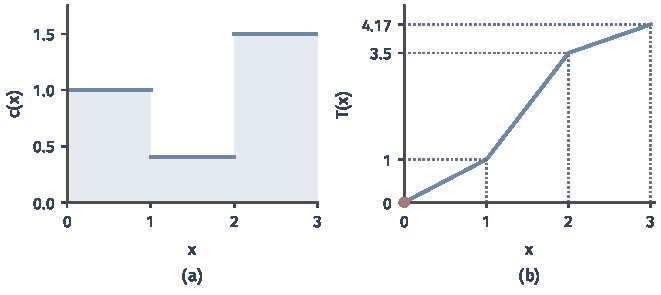
\includegraphics[width=112mm]{figures/06-differential-equations/02-partial-differential-equations/matplotlib/hj-arrival-1d/figure.pdf}
  \caption{一维到达时间。(a)分段常数的速度$c(x)$。(b)由$x=0$（红点）出发的到达时间$T(x)$，各段斜率是$1/c$。}
  \label{fig:hj-arrival-1d}
\end{BookInlineFigure}

到了高维，时刻$t$的波前是等值面$\{T=t\}$，已经被扫过的区域是$\{T\leq t\}$。设波前沿法向以速度$c(\bm{x})$推进。图~\ref{fig:hj-front-normal}中，点$\bm{x}$在$\mathrm{d}t$后沿法向$\bm{n}$到达$\bm{x}+c\,\mathrm{d}t\,\bm{n}$，那里的到达时间恰好多了$\mathrm{d}t$，所以
\[
  \langle\nabla T,\ c\,\bm{n}\rangle\,\mathrm{d}t=\mathrm{d}t.
\]
法向是$T$增长的方向，$\bm{n}=\nabla T/\lVert\nabla T\rVert_2$。代入后得到$c\,\lVert\nabla T\rVert_2=1$。

\begin{BookInlineFigure}
  \centering
  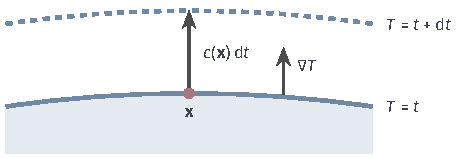
\includegraphics[width=78.3mm]{figures/06-differential-equations/02-partial-differential-equations/tikz/hj-front-normal/figure.pdf}
  \caption{波前的法向推进。实线是时刻$t$的波前，虚线是$t+\mathrm{d}t$的波前，浅蓝是已扫过的区域。两条等值线的法向距离是$c(\bm{x})\,\mathrm{d}t$，所以$\nabla T$的长度是$1/c$。}
  \label{fig:hj-front-normal}
\end{BookInlineFigure}

这个局部关系连同“从哪里开始、何时开始”的数据，构成到达时间问题。

\begin{definition}[程函方程]
\label{def:hj-eikonal}
设$\Omega\subset\mathbb{R}^{d}$是开集，$c:\Omega\to(0,\infty)$连续，$\Gamma\subset\overline{\Omega}$是闭集，$g:\Gamma\to\mathbb{R}$是给定的起始时刻。称
\begin{equation}
  c(\bm{x})\,\lVert\nabla T(\bm{x})\rVert_2=1\quad(\bm{x}\in\Omega\setminus\Gamma),\qquad
  T=g\quad\text{在}\ \Gamma\ \text{上}
  \label{eq:hj-eikonal}
\end{equation}
为\term{程函方程}（eikonal equation）的边值问题，$T$称为\term{到达时间}（arrival time），它的等值面$\{T=t\}$称为时刻$t$的\term{波前}（wavefront）。
\end{definition}

方程里没有时间，时间是未知函数的取值。一维时方程写作$\lvert T'\rvert=1/c$，比前面的$T'=1/c$少了方向信息：向左走还是向右走，方程本身不管。第~\ref{chap:pde-problems}章已经见过这种缺失带来的后果，$\lvert u'\rvert=1$、$u(\pm1)=0$没有$C^1$解，却有无穷多条几乎处处满足方程的锯齿线。

\paragraph{初值演化}
到达时间也可以放进一个随时间变化的场里。令$u(\bm{x},t)=T(\bm{x})-t$，则时刻$t$的波前就是$u(\cdot,t)$的零等值面。这时$\partial_tu=-1$，$\nabla u=\nabla T$，所以程函方程变成
\[
  \partial_tu+c(\bm{x})\,\lVert\nabla u\rVert_2=0.
\]
图~\ref{fig:hj-level-set}对$T(x)=\lvert x\rvert$画出这件事：函数图像整体下降，零点（红）就是向两侧跑的波前。

\begin{BookInlineFigure}
  \centering
  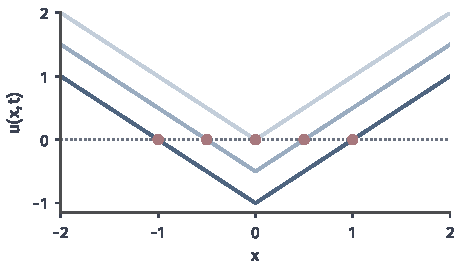
\includegraphics[width=78mm]{figures/06-differential-equations/02-partial-differential-equations/matplotlib/hj-level-set/figure.pdf}
  \caption{把波前写成零等值面。蓝色由浅到深是$u(x,t)=\lvert x\rvert-t$在$t=0,0.5,1$的图像，红点是零点$x=\pm t$，它们以速度$1$向两侧运动。}
  \label{fig:hj-level-set}
\end{BookInlineFigure}

把$c\lVert\bm{p}\rVert_2$换成一般的函数，就得到本章的第二类问题。

\begin{definition}[Hamilton--Jacobi初值问题]
\label{def:hj-ivp}
设$t_{\mathrm{f}}>0$，函数$H(t,\bm{x},\bm{p})$在$t\in[0,t_{\mathrm{f}}]$、$\bm{x},\bm{p}\in\mathbb{R}^{d}$上连续，$u_0$在$\mathbb{R}^{d}$上连续。称
\begin{equation}
  \partial_tu+H(t,\bm{x},\nabla u)=0\quad(\bm{x}\in\mathbb{R}^{d},\ 0<t<t_{\mathrm{f}}),\qquad
  u(\bm{x},0)=u_0(\bm{x})
  \label{eq:hj-ivp}
\end{equation}
为\term{Hamilton--Jacobi方程}（Hamilton--Jacobi equation）的初值问题，$H(t,\bm{x},\bm{p})$称为\term{Hamilton量}（Hamiltonian）。若$u$连续可微并逐点满足方程，就称$u$是经典解。
\end{definition}

本章的$u$只在$H$中通过梯度出现，$H$不依赖场值。比第~\ref{chap:transport-equations}章多出来的是：$H$对$\bm{p}$可以是非线性的。输运方程$\partial_tu+\langle\bm{v},\nabla u\rangle=0$正是$H=\langle\bm{v},\bm{p}\rangle$的线性情形。

\paragraph{Hamilton量的作用}
$H$回答的问题是：斜率为$\bm{p}$的地方，高度以多快的速度下降。这一点在平面解上能直接看出。对只依赖$\bm{p}$的$H$，令
\begin{equation}
  u(\bm{x},t)=\langle\bm{p},\bm{x}\rangle-tH(\bm{p}).
  \label{eq:hj-plane-solution}
\end{equation}
此时$\nabla u=\bm{p}$，$\partial_tu=-H(\bm{p})$，方程逐点成立。斜率不变，整个平面以速率$H(\bm{p})$下降。

图~\ref{fig:hj-plane-slopes}取$H(p)=p^2/2$。斜率$p=0,1,2$的三条直线在$t=1$时分别下降$0$、$0.5$和$2$。下降量对斜率是二次的。把两个斜率为$1$的解相加，得到的直线斜率为$2$，下降量却只有$1$，而斜率为$2$的解应当下降$2$，所以解不能叠加。

\begin{BookInlineFigure}
  \centering
  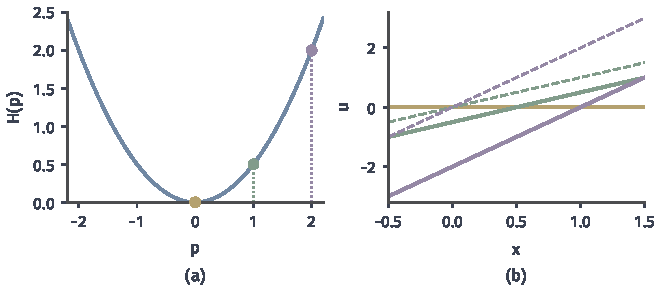
\includegraphics[width=112mm]{figures/06-differential-equations/02-partial-differential-equations/matplotlib/hj-plane-slopes/figure.pdf}
  \caption{Hamilton量决定下降速率。(a)$H(p)=p^2/2$，三个点对应$p=0,1,2$（黄、绿、紫）。(b)对应的平面解，虚线是$t=0$，实线是$t=1$，下降量分别是$0$、$0.5$、$2$。}
  \label{fig:hj-plane-slopes}
\end{BookInlineFigure}

一维时方程和第~\ref{chap:scalar-conservation-laws}章的守恒律有直接的关系。设$H=H(p)$，$u$足够光滑，对$\partial_tu+H(\partial_xu)=0$再求一次$x$偏导，$v=\partial_xu$满足
\[
  \partial_tv+\partial_xH(v)=0.
\]
所以一维的Hamilton--Jacobi方程是通量为$H$的标量守恒律的“原函数”，$u$的折角对应$v$的间断。这个对应后面会反复用到，但它只在一维成立；高维时梯度是向量，不满足标量守恒律。

\paragraph{两类问题需要的数据}
表~\ref{tab:hj-two-problems}把两类问题放在一起。两者都是对梯度的非线性方程，数据的位置和要求不同。

\begin{BookInlineTable}
  \centering
  \begin{tabular}{lll}
    \toprule
    & 到达时间问题 & 初值演化问题\\
    \midrule
    未知量 & $T(\bm{x})$，时间是取值 & $u(\bm{x},t)$\\
    梯度的含义 & 慢度向量，长度$1/c$ & 局部斜率\\
    方程的作用 & 限制梯度的长度 & 由斜率给出下降速率\\
    所需数据 & 源集合$\Gamma$上的起始时刻 & $t=0$时整个$\mathbb{R}^{d}$上的$u_0$\\
    数据的限制 & 起始时刻不能相互矛盾 & 增长和正则性\\
    \bottomrule
  \end{tabular}
  \caption{到达时间问题与初值演化问题的对比。}
  \label{tab:hj-two-problems}
\end{BookInlineTable}

初值问题只需要在$t=0$给一个函数，方程对时间是一阶的，不需要初始速度，全空间上也没有侧边界。到达时间问题的数据要彼此相容。在区间$(0,1)$上取$c=1$，两端都是源，起始时刻为$g(0)=0$和$g(1)=2$。从左端出发的波前在时刻$1$就到达了右端，而右端规定的起始时刻是$2$，这个规定不会起作用。一般的要求是，$\lvert g(\bm{x})-g(\bm{y})\rvert$不超过两点之间的传播时间；这个限制在第~\ref{sec:hj-comparison}节还要用到。

\section{特征方程}
\label{sec:hj-characteristics}

方程只说了时间导数和梯度的关系，能否沿某些曲线把它化成常微分方程？输运方程已经用过这个办法：沿速度场的轨线，解的值不变。这里的困难在于，方程对梯度非线性，沿曲线求导时会冒出二阶导数。这一节要找到让二阶导数消失的曲线，并说明怎样从这些曲线重建场。

\paragraph{沿什么曲线求导}
设$H$二阶连续可微，$u$是二阶连续可微的经典解。取一条待定的曲线$\bm{x}(s)$，记沿线的梯度和值为
\[
  \bm{p}(s)=\nabla u(\bm{x}(s),s),\qquad z(s)=u(\bm{x}(s),s).
\]
对$\bm{p}$求导，用链式法则，得到
\[
  \dot{\bm{p}}=\partial_t\nabla u+\nabla^2u\,\dot{\bm{x}}.
\]
这里出现了未知的二阶导数$\nabla^2u$，这是方程非线性的代价。

为消去$\partial_t\nabla u$，对方程本身关于$\bm{x}$求梯度：
\[
  \partial_t\nabla u+\nabla_{\bm{x}}H+\nabla^2u\,\nabla_{\bm{p}}H=0.
\]
两式相减消去$\partial_t\nabla u$，得到
\[
  \dot{\bm{p}}=-\nabla_{\bm{x}}H+\nabla^2u\,\bigl(\dot{\bm{x}}-\nabla_{\bm{p}}H\bigr).
\]
括号里的量可以由我们选择：只要曲线满足$\dot{\bm{x}}=\nabla_{\bm{p}}H$，二阶导数就消失了。曲线的方向不是事先给定的速度场，而由当地的斜率决定。

再算沿线的值。由链式法则和方程，
\[
  \dot{z}=\partial_tu+\langle\nabla u,\dot{\bm{x}}\rangle=-H+\langle\bm{p},\nabla_{\bm{p}}H\rangle.
\]
把这三个结果写在一起。

\begin{theorem}[特征方程组]
\label{thm:hj-characteristics}
设$H\in C^2$，$u\in C^2$是方程$\partial_tu+H(t,\bm{x},\nabla u)=0$的解。若曲线$\bm{x}(s)$的速度等于$\nabla_{\bm{p}}H$（梯度变量取沿线的$\nabla u$），则沿线的梯度$\bm{p}(s)$和值$z(s)$满足
\begin{equation}
  \dot{\bm{x}}=\nabla_{\bm{p}}H,\qquad
  \dot{\bm{p}}=-\nabla_{\bm{x}}H,\qquad
  \dot{z}=\langle\bm{p},\nabla_{\bm{p}}H\rangle-H,
  \label{eq:hj-characteristics}
\end{equation}
其中$H$及其偏导数都在$(s,\bm{x}(s),\bm{p}(s))$处取值。这组常微分方程称为\term{特征方程组}（characteristic system），$\bm{x}(s)$称为特征线。
\end{theorem}

式~\eqref{eq:hj-characteristics}的前两个方程不含$z$，构成$(\bm{x},\bm{p})$空间中的闭合系统，这就是第~\ref{chap:ode-sensitivity}章的Hamilton方程。在那里我们已经知道它生成的流保持相空间体积，$H$不显含时间时沿轨道守恒。这两条性质这里不再重复；本章的新内容是第三个方程，它在已知$(\bm{x},\bm{p})$之后只是一次积分，负责把值带上。

图~\ref{fig:hj-characteristic-lift}是一条特征线的示意。出发点$\bm{y}$提供初始斜率$\bm{p}_0=\nabla u_0(\bm{y})$，此后位置按$\nabla_{\bm{p}}H$前进，斜率按$-\nabla_{\bm{x}}H$变化，值按第三式累积。

\begin{BookInlineFigure}
  \centering
  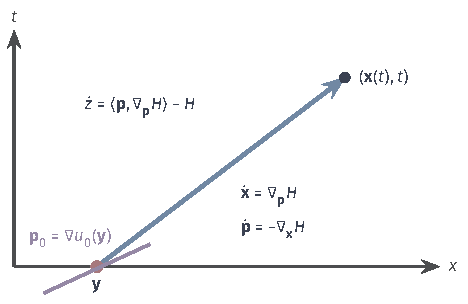
\includegraphics[width=79.3mm]{figures/06-differential-equations/02-partial-differential-equations/tikz/hj-characteristic-lift/figure.pdf}
  \caption{一条特征线（蓝）。从初始点$\bm{y}$（红）出发，紫线表示初值在该点的切线，它给出初始斜率$\bm{p}_0$。沿线要同时求解位置、斜率和值三个量。}
  \label{fig:hj-characteristic-lift}
\end{BookInlineFigure}

\paragraph{由特征重建场}
定理~\ref{thm:hj-characteristics}假定解已经存在，只是必要条件。反过来，给定$u_0$，能否从特征线造出解？做法分三步。

\begin{enumerate}
  \item 对每个$\bm{y}$，从位置$\bm{y}$、斜率$\nabla u_0(\bm{y})$、值$u_0(\bm{y})$出发解式~\eqref{eq:hj-characteristics}，得到$\bm{x}(\bm{y},t)$、$\bm{p}(\bm{y},t)$、$z(\bm{y},t)$。
  \item 对给定的$(\bm{x},t)$，解方程$\bm{x}(\bm{y},t)=\bm{x}$，求出是哪条特征线到达这里。
  \item 令$u(\bm{x},t)=z(\bm{y},t)$，其中$\bm{y}$是上一步的解。
\end{enumerate}

第二步是关键：只有映射$\bm{y}\mapsto\bm{x}(\bm{y},t)$可逆时，$u$才有定义。$t=0$时它是恒等映射，所以短时间内可逆，这用到反函数定理：Jacobian可逆的连续可微映射局部有连续可微的逆，可参考\BookChapterRef{chap:implicit-inverse-functions}{卷二第22章“隐函数与反函数”}。这一步还需要证明造出来的函数确实满足方程，而不只是沿线有正确的取值。

\begin{theorem}[经典解的局部存在]
\label{thm:hj-local-classical}
设$H\in C^2$，$u_0\in C^2$。对每个$\bm{y}_0\in\mathbb{R}^{d}$，存在$t_1>0$和$\bm{y}_0$的邻域，使上面三步在$\bm{x}(\bm{y}_0,t)$附近、$0\leq t<t_1$时定义出一个连续可微函数$u$，它满足
\begin{equation}
  \partial_tu+H(t,\bm{x},\nabla u)=0,\qquad u(\cdot,0)=u_0,\qquad\nabla u(\bm{x}(\bm{y},t),t)=\bm{p}(\bm{y},t).
  \label{eq:hj-local-classical}
\end{equation}
\end{theorem}

\begin{proof}
式~\eqref{eq:hj-characteristics}的右端关于$(\bm{x},\bm{p})$连续可微，初值关于$\bm{y}$连续可微，所以解关于$\bm{y}$连续可微。映射$(\bm{y},t)\mapsto(\bm{x}(\bm{y},t),t)$在$t=0$处的Jacobian是单位阵，由反函数定理局部可逆，$u$有定义且连续可微。

关键是证明$\nabla u=\bm{p}$。固定指标$i$，记$\partial_i=\partial/\partial y_i$，考虑
\[
  a(t)=\partial_iz-\langle\bm{p},\partial_i\bm{x}\rangle.
\]
$t=0$时，$\partial_iz=\partial_iu_0(\bm{y})$，$\partial_i\bm{x}=\bm{e}_i$，$\bm{p}=\nabla u_0(\bm{y})$，所以$a(0)=0$。

下面计算$\dot{a}$。对$\dot{z}=\langle\bm{p},\nabla_{\bm{p}}H\rangle-H$关于$y_i$求导，其中含$\partial_i\bm{p}$的两项抵消：
\[
  \partial_i\dot{z}=\langle\bm{p},\partial_i(\nabla_{\bm{p}}H)\rangle-\langle\nabla_{\bm{x}}H,\partial_i\bm{x}\rangle.
\]
另一方面，由$\dot{\bm{p}}=-\nabla_{\bm{x}}H$和$\dot{\bm{x}}=\nabla_{\bm{p}}H$，
\[
  \frac{\mathrm{d}}{\mathrm{d}t}\langle\bm{p},\partial_i\bm{x}\rangle=-\langle\nabla_{\bm{x}}H,\partial_i\bm{x}\rangle+\langle\bm{p},\partial_i(\nabla_{\bm{p}}H)\rangle.
\]
两式相减，$\dot{a}=0$，于是$a\equiv0$，即对所有$i$有$\partial_iz=\langle\bm{p},\partial_i\bm{x}\rangle$。

由$u$的定义和链式法则，又有
\[
  \partial_iz=\langle\nabla u,\partial_i\bm{x}\rangle.
\]
比较两式，得
\[
  \langle\nabla u-\bm{p},\partial_i\bm{x}\rangle=0,\qquad i=1,\ldots,d.
\]
向量$\partial_1\bm{x},\ldots,\partial_d\bm{x}$线性无关，所以$\nabla u=\bm{p}$。

最后对$z(\bm{y},t)=u(\bm{x}(\bm{y},t),t)$关于$t$求导，并代入$\dot{z}$的方程和$\nabla u=\bm{p}$：
\[
  \langle\bm{p},\nabla_{\bm{p}}H\rangle-H=\partial_tu+\langle\bm{p},\nabla_{\bm{p}}H\rangle.
\]
消去相同的项，得到$\partial_tu=-H$。
\end{proof}

下面用一个可以手算的例子走一遍这三步。这个例子会贯穿到最后一节。

\begin{example}[余弦初值]
\label{ex:hj-cos}
取$d=1$，$H(p)=p^2/2$，$u_0(x)=\cos x$。特征方程组是
\[
  \dot{x}=p,\qquad\dot{p}=0,\qquad\dot{z}=\frac{p^2}{2}.
\]
从$y$出发，初始斜率$p=-\sin y$沿线不变，特征线是直线，于是
\[
  x=y-t\sin y,\qquad p=-\sin y,\qquad z=\cos y+\frac{t}{2}\sin^2y.
\]

取$t=1/2$、$y=\pi/2$，得到
\[
  x=\frac{\pi}{2}-\frac12,\qquad p=-1,\qquad z=\frac14.
\]
因此$u(\pi/2-1/2,\ 1/2)=1/4$，该点的斜率是$-1$。$t=1/2$时$\partial x/\partial y=1-\frac12\cos y>0$，$y\mapsto x$严格单调，这个点只由这一条特征线到达。
\end{example}

\paragraph{到达时间的特征线}
对波前对应的$H(\bm{x},\bm{p})=c(\bm{x})\lVert\bm{p}\rVert_2$（$\bm{p}\neq\bm{0}$），偏导数是
\[
  \nabla_{\bm{p}}H=c\,\frac{\bm{p}}{\lVert\bm{p}\rVert_2},\qquad\nabla_{\bm{x}}H=\lVert\bm{p}\rVert_2\nabla c.
\]
代入式~\eqref{eq:hj-characteristics}，第一个方程说特征线沿$\bm{p}$的方向以速度$c$前进，这条曲线叫射线。第三个方程给出
\[
  \dot{z}=\Bigl\langle\bm{p},c\frac{\bm{p}}{\lVert\bm{p}\rVert_2}\Bigr\rangle-c\lVert\bm{p}\rVert_2=0.
\]
也就是说，$u=T-t$沿射线不变，这正是波前的含义：射线上的点时刻$s$恰好在波前上，$T(\bm{x}(s))$每经过单位时间增加$1$。

图~\ref{fig:hj-huygens}从另一个角度解释射线。把当前波前上的每个点当作新的小波源，小圆的公共包络就是下一时刻的波前，连接圆心和切点的方向就是射线方向。这就是几何上的波前图景，也说明射线垂直于波前（速度$c$只依赖位置时）。

\begin{BookInlineFigure}
  \centering
  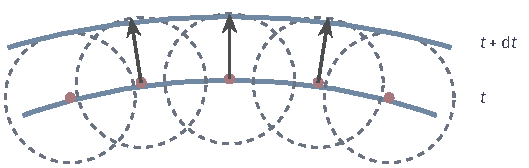
\includegraphics[width=89.5mm]{figures/06-differential-equations/02-partial-differential-equations/tikz/hj-huygens/figure.pdf}
  \caption{波前的包络图景。下方蓝线是时刻$t$的波前，红点发出半径$c\,\mathrm{d}t$的小圆（虚线），上方蓝线是这些小圆的包络，即$t+\mathrm{d}t$的波前，深灰箭头是射线。}
  \label{fig:hj-huygens}
\end{BookInlineFigure}

速度为常数时，$\nabla c=\bm{0}$，$\bm{p}$不变，射线是直线，$T$就是到源点的距离除以$c$。速度随位置变化时射线弯曲。例如在平面上取$c(\bm{x})=1+ax_2$，$a=1/2$，源在原点。这个速度下到达时间有闭式
\begin{equation}
  T(\bm{x})=\frac{1}{a}\operatorname{arccosh}\Bigl(1+\frac{a^2\lVert\bm{x}\rVert_2^2}{2c(\bm{x})}\Bigr),
  \label{eq:hj-linear-speed}
\end{equation}
代入程函方程可以验证。我们沿竖直射线手算一个点：在$x_1=0$上向上走，$\dot{x}_2=1+x_2/2$，$x_2(0)=0$，解得
\[
  x_2(t)=2\bigl(\mathrm{e}^{t/2}-1\bigr).
\]
令$x_2=2$，得到$t=2\ln2\approx1.386$。式~\eqref{eq:hj-linear-speed}在$(0,2)$处给出$\operatorname{arccosh}(1.25)/a=2\ln2$，两者一致。

图~\ref{fig:hj-rays-linear-speed}用数值积分解特征方程组，得到射线，再画上式~\eqref{eq:hj-linear-speed}的等值线。射线总向速度小的一侧弯转，斜向上出发的射线进入快层后又折回下方。射线与等值线处处垂直。积分到$t=3.2$时，射线终点的$T$值与$t$的差不超过$2\times10^{-11}$。

\begin{BookInlineFigure}
  \centering
  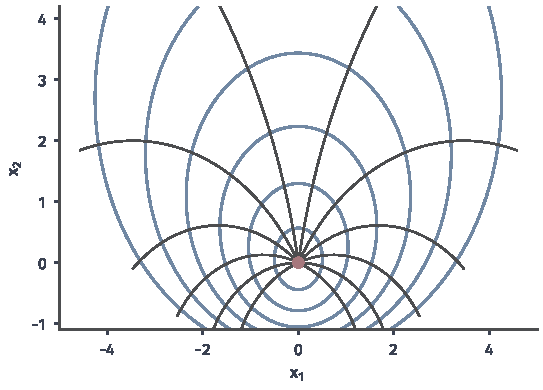
\includegraphics[width=92mm]{figures/06-differential-equations/02-partial-differential-equations/matplotlib/hj-rays-linear-speed/figure.pdf}
  \caption{速度$c=1+x_2/2$下从原点（红）出发的波前和射线。蓝线是式~\eqref{eq:hj-linear-speed}在$T=0.5,1,\ldots,3$的等值线，深灰线是用步长$0.01$的四阶Runge--Kutta方法积分特征方程组得到的射线，初始方向间隔$20^\circ$。}
  \label{fig:hj-rays-linear-speed}
\end{BookInlineFigure}

\paragraph{边界数据怎样启动特征线}
初值问题的特征线从每个$\bm{y}$以确定的斜率出发。程函方程的数据只在$\Gamma$上给出值，切向导数能由$g$算出，法向导数却要由方程决定。设$\Gamma$是一段超曲面，$\nabla_\Gamma g$是$g$沿$\Gamma$的切向梯度，$\bm{n}$是单位法向。令$\bm{p}=\nabla_\Gamma g+\beta\bm{n}$，代入$\lVert\bm{p}\rVert_2=1/c$，得到
\begin{equation}
  \beta=\pm\sqrt{\frac{1}{c^2}-\lVert\nabla_\Gamma g\rVert_2^2}.
  \label{eq:hj-boundary-branches}
\end{equation}
图~\ref{fig:hj-boundary-branches}的圆是$\lVert\bm{p}\rVert_2=1/c$，竖直虚线是切向分量固定时的所有候选，两个交点就是式~\eqref{eq:hj-boundary-branches}的两支。

\begin{BookInlineFigure}
  \centering
  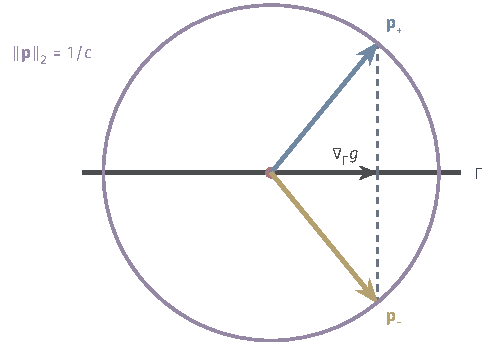
\includegraphics[width=83.5mm]{figures/06-differential-equations/02-partial-differential-equations/tikz/hj-boundary-branches/figure.pdf}
  \caption{边界上的初始斜率。紫圆是$\lVert\bm{p}\rVert_2=1/c$，水平线是边界$\Gamma$，切向分量$\nabla_\Gamma g$由数据给定，方程留下两支法向分量：$\bm{p}_+$（蓝）指向一侧，$\bm{p}_-$（黄）指向另一侧。}
  \label{fig:hj-boundary-branches}
\end{BookInlineFigure}

要使两支是不同的实数，需要$\lVert\nabla_\Gamma g\rVert_2<1/c$。它的含义是：起始时刻沿$\Gamma$变化得不能太快。沿$\Gamma$的视在传播速度$1/\lVert\nabla_\Gamma g\rVert_2$要大于当地的波速$c$。若$g$沿$\Gamma$变化得更快，某个点规定的起始时刻已晚于别的点传来的波前，就是第~\ref{sec:hj-problem}节$g(1)=2$的情形。选定一支后，就得到从$\Gamma$的一侧发出的波前。

\section{尖点的产生}
\label{sec:hj-cusps}

定理~\ref{thm:hj-local-classical}只保证短时间内有解。时间一长，映射$\bm{y}\mapsto\bm{x}(\bm{y},t)$可能不再可逆，同一个位置会被几条特征线到达。这时经典解到了尽头，而且仅仅要求方程几乎处处成立，也无法决定接下来该怎么办。

\paragraph{梯度沿特征线的变化}
取$d=1$，$H=H(p)$。此时$\dot{p}=-\partial_xH=0$，斜率沿特征线不变，特征线是直线：
\[
  x(y,t)=y+tH'\bigl(u_0'(y)\bigr).
\]
对$y$求导，记$a(y)=H''(u_0'(y))\,u_0''(y)$，得到
\[
  \partial_yx=1+ta(y).
\]

二阶导数$w=\partial_x^2u$沿特征线的取值，可以用$\partial_yp/\partial_yx$算出。由$p=u_0'(y)$，
\begin{equation}
  w(y,t)=\frac{u_0''(y)}{1+ta(y)}.
  \label{eq:hj-riccati}
\end{equation}
若$H$是严格凸的，$a(y)<0$恰好发生在$u_0''(y)<0$的地方，也就是初值向下弯的地方。这些地方的分母随时间减小，到$t=-1/a(y)$时变成零，曲率发散。

\begin{theorem}[经典解的首次失效]
\label{thm:hj-breakdown}
设$d=1$，$H\in C^2$，$u_0\in C^2$，且$u_0'$、$u_0''$有界，$H''$在$u_0'$的值域上有界。记$m=\inf_ya(y)$。

若$m\geq0$，令$t^*=\infty$；若$m<0$，令$t^*=-1/m$。则在$0\leq t<t^*$上，$y\mapsto x(y,t)$是$\mathbb{R}$到$\mathbb{R}$的同胚，特征线给出整个$\mathbb{R}\times[0,t^*)$上的$C^2$解。若$m<0$且下确界在某点$y^*$处达到，则
\begin{equation}
  \lim_{t\uparrow t^*}\bigl\lvert\partial_x^2u(x(y^*,t),t)\bigr\rvert=\infty,
  \label{eq:hj-breakdown}
\end{equation}
所以这个解不能在$t^*$之后作为$C^2$解延拓。
\end{theorem}

\begin{proof}
设$0\leq t<t^*$。此时
\[
  \partial_yx=1+ta(y)\geq1+tm\geq\kappa>0,
\]
其中$m\geq0$时取$\kappa=1$，$m<0$时取$\kappa=1-t/t^*$。一阶导数有正下界，所以$y\mapsto x$严格递增，并且$\lvert x\rvert\to\infty$（$\lvert y\rvert\to\infty$时），是同胚。

在每个闭区间$[0,t_2]\subset[0,t^*)$上，$\kappa$有统一的正下界。逐点应用定理~\ref{thm:hj-local-classical}的计算，得到连续可微的$u$，且$\partial_xu=p$。由$w$的公式，$\partial_xu$关于$x$连续可微，$u$是$C^2$解。

式~\eqref{eq:hj-breakdown}由式~\eqref{eq:hj-riccati}得到：在$y=y^*$处，分母是$1+tm=1-t/t^*\to0$，分子$u_0''(y^*)$不为零（因为$a(y^*)=m<0$）。若存在$C^2$延拓，$\partial_x^2u$在紧集上有界，这与发散矛盾。
\end{proof}

定理说的是：斜率的变化率在有限时间内发散，而斜率和场值本身一直有界。这和第~\ref{chap:scalar-conservation-laws}章的结论对应，$v=\partial_xu$正是在同一时刻由光滑变成间断。

把定理用到例~\ref{ex:hj-cos}。$a(y)=u_0''(y)=-\cos y$，最小值$-1$在$y=0$处取得，所以$t^*=1$。特征线和曲率是
\[
  \partial_yx=1-t\cos y,\qquad w=\frac{-\cos y}{1-t\cos y}.
\]
在$x=0$（$y=0$）处，$w=-1/(1-t)$。$t=0.5$时曲率是$-2$，$t=0.9$时是$-10$。图~\ref{fig:hj-cos-steepening}显示$u$在原点越来越尖，斜率曲线越来越陡。

\begin{BookInlineFigure}
  \centering
  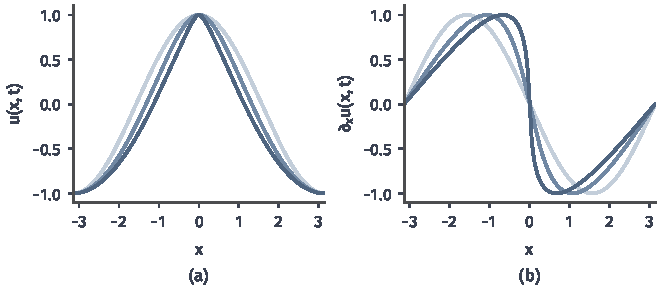
\includegraphics[width=112mm]{figures/06-differential-equations/02-partial-differential-equations/matplotlib/hj-cos-steepening/figure.pdf}
  \caption{$H=p^2/2$、$u_0=\cos x$的经典解，蓝色由浅到深是$t=0,0.5,0.9$。(a)场值$u$。(b)斜率$\partial_xu$，$x=0$处的斜率变化率是$-1/(1-t)$，$t\uparrow1$时发散，而斜率一直保持在$[-1,1]$内。}
  \label{fig:hj-cos-steepening}
\end{BookInlineFigure}

图~\ref{fig:hj-cos-characteristics}(a)把特征线全部画出来。$t<1$时它们互不相交，$t=1$时最先在红点相遇。条件$\partial_yx=0$给出特征线族的包络
\[
  t=\frac{1}{\cos y},\qquad x=y-\tan y,
\]
即图中的深灰曲线，称为\term{焦散线}（caustic）。两支焦散线之间的每个点都有三条特征线经过，这个区域由红点向上张开。

\begin{BookInlineFigure}
  \centering
  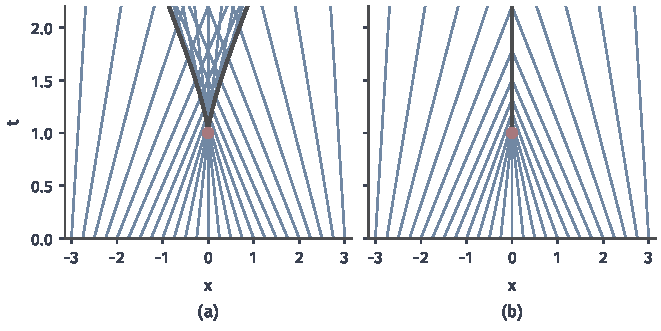
\includegraphics[width=112mm]{figures/06-differential-equations/02-partial-differential-equations/matplotlib/hj-cos-characteristics/figure.pdf}
  \caption{$u_0=\cos x$的特征线$x=y-t\sin y$（蓝）。(a)全部画出，它们在红点$(0,1)$首次相遇，深灰曲线是焦散线。(b)只画到撞上$x=0$（深灰粗线）为止的部分，第~\ref{sec:hj-hopf-lax}节将说明解用到的正是这一部分。}
  \label{fig:hj-cos-characteristics}
\end{BookInlineFigure}

\paragraph{同一位置的多个分支}
$t^*$之后，公式仍然能算，只是不再给出函数。取$t=\pi/2$、$x=0$，要求解
\[
  y=\frac{\pi}{2}\sin y.
\]
它有三个解$y=0$、$y=\pi/2$、$y=-\pi/2$。代入$p=-\sin y$和$z=\cos y+\frac{t}{2}\sin^2y$，得到
\[
  \begin{gathered}
    y=0:\quad(p,z)=(0,1),\\
    y=\tfrac{\pi}{2}:\quad(p,z)=(-1,\tfrac{\pi}{4}),\\
    y=-\tfrac{\pi}{2}:\quad(p,z)=(1,\tfrac{\pi}{4}).
  \end{gathered}
\]
三条特征线带来三对不同的斜率和值，$u(0,\pi/2)$应当取哪一个？特征方程组只负责沿线传递，回答不了这个问题。

图~\ref{fig:hj-swallowtail}(a)是$t=\pi/2$时$(x,z)$的像。曲线在$\lvert x\rvert\leq0.33$内折叠成三层，整条曲线不是函数图像。图(b)是相平面上$(x,p)$的像，初始的正弦曲线被Hamilton流剪切后折叠，同一个$x$上有三个$p$。蓝色画的是后面选出的解，下包络在$x=0$处有折角，斜率从$+1$跳到$-1$。

\begin{BookInlineFigure}
  \centering
  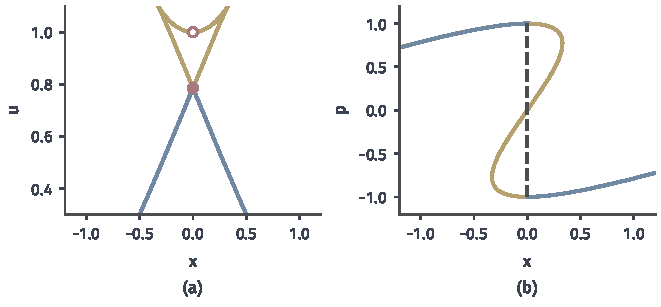
\includegraphics[width=112mm]{figures/06-differential-equations/02-partial-differential-equations/matplotlib/hj-swallowtail/figure.pdf}
  \caption{$t=\pi/2$时的多值像（黄）与选出的解（蓝）。(a)$(x,z)$平面，$x=0$处有三个值，红点是$\pi/4$（两条分支的公共值），空心点是$1$。(b)$(x,p)$平面，折叠的曲线在$x=0$处被虚线截断，蓝线在$x=0$处从$p=1$跳到$p=-1$。}
  \label{fig:hj-swallowtail}
\end{BookInlineFigure}

到达时间问题里，这个选择有明确的物理含义。平面上有两个源$\bm{a}=(-1,0)$和$\bm{b}=(1,0)$，时刻$0$同时点燃。每个源单独产生的到达时间是$T_1=\lVert\bm{x}-\bm{a}\rVert_2$和$T_2=\lVert\bm{x}-\bm{b}\rVert_2$，都是经典解。但一点只会被第一次到达的波前扫到，所以
\[
  T=\min\{T_1,T_2\}.
\]
后到的波前经过的是已经扫过的区域，没有意义。

图~\ref{fig:hj-two-sources}(a)显示两列圆形波前相遇后在中垂线上消失，$T$沿这条线不可微。在直线$x_2=1$上看，两条分支在$x_1=0$处都等于$\sqrt2$，斜率分别是$+1/\sqrt2$和$-1/\sqrt2$，取最小值后在该点形成折角，见图(b)。

\begin{BookInlineFigure}
  \centering
  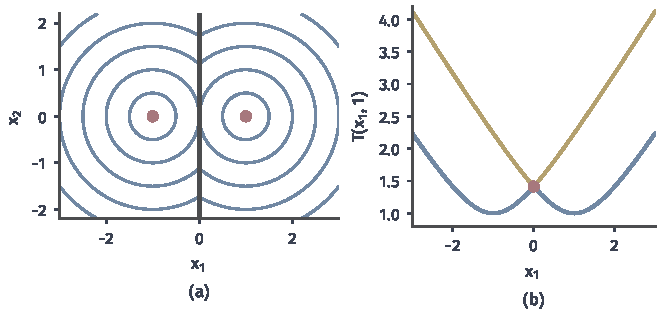
\includegraphics[width=112mm]{figures/06-differential-equations/02-partial-differential-equations/matplotlib/hj-two-sources/figure.pdf}
  \caption{两个同时点燃的源（红点）。(a)蓝线是$T=\min\{T_1,T_2\}$的等值线，深灰线是中垂线，两列波前在此相遇后消失。(b)沿$x_2=1$的截面，黄线是两个单独的到达时间，蓝线是取最小值的结果，红点是折角，高度$\sqrt2$。}
  \label{fig:hj-two-sources}
\end{BookInlineFigure}

这两个例子都选了较小的值。这究竟是巧合，还是方程本身的要求？下面的例子说明，光凭几乎处处的逐点检验回答不了。

\paragraph{几乎处处满足方程仍然不够}
取$H=p^2/2$，$u_0=0$。$u\equiv0$满足方程和初值。还有没有别的连续解？令
\begin{equation}
  w(x,t)=\min\Bigl\{\lvert x\rvert-\frac{t}{2},\ 0\Bigr\}.
  \label{eq:hj-notch}
\end{equation}
它的形状是一个越挖越深的凹槽，在$\lvert x\rvert\geq t/2$上等于$0$，在$\lvert x\rvert<t/2$上等于$\lvert x\rvert-t/2$。

逐块验证。在$\lvert x\rvert>t/2$上$w=0$，方程成立。在$0<\lvert x\rvert<t/2$上$\partial_xw=\pm1$，$\partial_tw=-1/2$，所以
\[
  \partial_tw+\frac12(\partial_xw)^2=-\frac12+\frac12=0.
\]
除了三条线$x=0$、$x=\pm t/2$，方程都成立，这三条线的测度为零。初值也满足。于是$w$和$0$是同一个初值问题的两个几乎处处解，见图~\ref{fig:hj-notch}(a)。

图~\ref{fig:hj-notch}(b)把凹槽翻译成斜率。$v=\partial_xw$在$x=\pm t/2$处的跳跃满足Rankine--Hugoniot条件，例如$x=t/2$处左值$1$、右值$0$，通量$v^2/2$给出速度$1/2$。而在$x=0$处，$v$从$-1$跳到$+1$，这是左值小于右值的间断。第~\ref{chap:scalar-conservation-laws}章的熵条件说，凸通量下的间断必须左值大于右值，否则特征线会从间断面向外分开。$x=0$处的跳跃正好违反这一条。

\begin{BookInlineFigure}
  \centering
  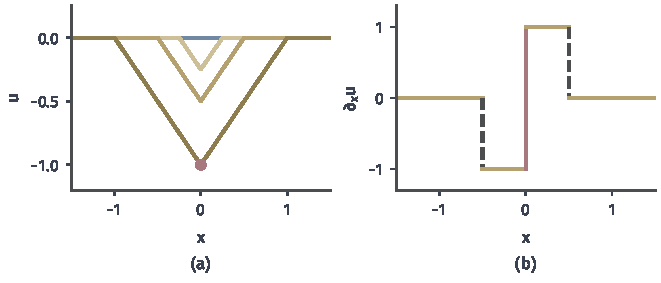
\includegraphics[width=112mm]{figures/06-differential-equations/02-partial-differential-equations/matplotlib/hj-notch/figure.pdf}
  \caption{初值为$0$时的非唯一性。(a)蓝线是$u=0$，黄色由浅到深是式~\eqref{eq:hj-notch}的$w$在$t=0.5,1,2$的图像，红点是底部折角。(b)$t=1$时的斜率$\partial_xw$，深灰虚线处的跳跃左值大于右值，红线处的跳跃左值小于右值。}
  \label{fig:hj-notch}
\end{BookInlineFigure}

因此，光用“几乎处处”这条标准，经典解失效后方程给不出答案。需要在不可微的点上也提出要求，而且要求必须能区分$w$底部的折角和$T$的尖峰。这是下一节的任务。

\section{黏性解}
\label{sec:hj-viscosity}

折角处没有导数，方程不能代入。能否用一些有导数的东西替代它？答案是拿光滑函数从上方或下方贴住$u$，把方程写在贴住的光滑函数上。

\paragraph{用光滑函数从两侧接触}
设$\varphi$是光滑函数，$u-\varphi$在点$\bm{x}_0$有局部极大值。几何上，把$\varphi$上下平移，使它在$\bm{x}_0$处与$u$相等，那么附近有$\varphi\geq u$，$\varphi$从上方贴住$u$。若$u$在$\bm{x}_0$可微，极值点的一阶条件给出$\nabla\varphi(\bm{x}_0)=\nabla u(\bm{x}_0)$。这样可以从$\varphi$读出$u$的梯度。

$u$不可微时，情况由折角的方向决定。图~\ref{fig:hj-touching}画了三种情形。在光滑点上，从上方和下方都能贴住，贴住的函数斜率都等于$u$的斜率。在向下弯的折角（凹折角）处，从上方可以用多种斜率贴住，从下方则根本贴不住。在向上弯的折角（凸折角）处正好相反。

\begin{BookInlineFigure}
  \centering
  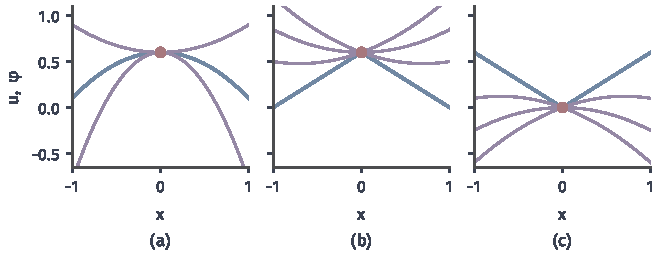
\includegraphics[width=112mm]{figures/06-differential-equations/02-partial-differential-equations/matplotlib/hj-touching/figure.pdf}
  \caption{光滑测试函数（紫）在红点贴住$u$（蓝）。(a)光滑点：上下两侧都能贴住，斜率唯一。(b)凹折角：只能从上方贴住，斜率可取一个区间。(c)凸折角：只能从下方贴住，斜率可取一个区间。}
  \label{fig:hj-touching}
\end{BookInlineFigure}

接下来决定不等式的方向。设$u_\varepsilon$是$\partial_tu+H(\nabla u)=\varepsilon\Delta u$的光滑解，$\varepsilon>0$，且$u_\varepsilon-\varphi$在内部点取局部极大。一阶条件和二阶条件给出
\[
  \partial_t\varphi=\partial_tu_\varepsilon,\qquad\nabla\varphi=\nabla u_\varepsilon,\qquad\Delta u_\varepsilon\leq\Delta\varphi.
\]
代入方程，得到
\[
  \partial_t\varphi+H(\nabla\varphi)=\varepsilon\Delta u_\varepsilon\leq\varepsilon\Delta\varphi.
\]
令$\varepsilon\to0$，右端趋于零。所以从上方贴时，自然的要求是$\partial_t\varphi+H(\nabla\varphi)\leq0$；从下方贴时不等号反向。这个计算只是启示，严格的结论在第~\ref{sec:hj-vanishing}节证明，但它已经给出了定义的形状。

\begin{definition}[黏性解]
\label{def:hj-viscosity}
设$u\in C(\mathbb{R}^{d}\times[0,t_{\mathrm{f}}))$。若对每个$\varphi\in C^1(\mathbb{R}^{d}\times(0,t_{\mathrm{f}}))$，当$u-\varphi$在$(\bm{x}_0,t_0)$（$t_0>0$）取局部极大值时都有
\begin{equation}
  \partial_t\varphi(\bm{x}_0,t_0)+H\bigl(t_0,\bm{x}_0,\nabla\varphi(\bm{x}_0,t_0)\bigr)\leq0,
  \label{eq:hj-subsolution}
\end{equation}
就称$u$是式~\eqref{eq:hj-ivp}中方程的\term{黏性次解}（viscosity subsolution）。若对每个这样的$\varphi$，当$u-\varphi$在$(\bm{x}_0,t_0)$取局部极小值时都有
\begin{equation}
  \partial_t\varphi(\bm{x}_0,t_0)+H\bigl(t_0,\bm{x}_0,\nabla\varphi(\bm{x}_0,t_0)\bigr)\geq0,
  \label{eq:hj-supersolution}
\end{equation}
就称$u$是\term{黏性上解}（viscosity supersolution）。既是次解又是上解的函数称为黏性解。初值问题的黏性解还要求$u(\cdot,0)=u_0$。
\end{definition}

记忆方式是：次解贴上方，得到“小于等于”；上解贴下方，得到“大于等于”。这个定义里从头到尾没有$u$的导数，所以它对连续函数有意义。

稳态方程$F(\bm{x},\nabla u)=0$的定义完全相同：局部极大处要求$F(\bm{x}_0,\nabla\varphi)\leq0$，局部极小处要求$F(\bm{x}_0,\nabla\varphi)\geq0$，边界条件单独提出。到达时间问题取
\[
  F(\bm{x},\bm{p})=c(\bm{x})\lVert\bm{p}\rVert_2-1.
\]

定义要有用，首先不能把经典解排除在外，而且不可微的地方之外应当和原方程一致。

\begin{lemma}[与经典解相容]
\label{lem:hj-consistency}
(1)连续可微的经典解是黏性解。(2)若黏性解$u$在内部点$\bm{z}_0=(\bm{x}_0,t_0)$可微，则方程在$\bm{z}_0$处逐点成立，即
\begin{equation}
  \partial_tu(\bm{z}_0)+H\bigl(t_0,\bm{x}_0,\nabla u(\bm{z}_0)\bigr)=0.
  \label{eq:hj-consistency}
\end{equation}
\end{lemma}

\begin{proof}
(1)若$u\in C^1$，$u-\varphi$在内部取极值，则$\partial_t\varphi=\partial_tu$，$\nabla\varphi=\nabla u$，代入方程得到等号，两个不等式都成立。

(2)只需构造一个$C^1$函数从上方贴住$u$且导数与$u$相同，下方同理，再分别代入两个定义。记$r=\lVert\bm{z}-\bm{z}_0\rVert_2$，并令$v$为$u$减去它在$\bm{z}_0$的一阶Taylor多项式。由可微性，
\[
  \rho(r)=\max_{\lVert\bm{z}-\bm{z}_0\rVert_2\leq r}\frac{\lvert v(\bm{z})\rvert}{\lVert\bm{z}-\bm{z}_0\rVert_2}
\]
连续、不减，且$\rho(0)=0$（规定分式在$\bm{z}=\bm{z}_0$处取$0$）。令
\[
  \psi(\bm{z})=\int_r^{2r}\rho(\tau)\,\mathrm{d}\tau.
\]

$\rho$连续，所以$\psi$在$\bm{z}\neq\bm{z}_0$处$C^1$。又$\lvert\psi\rvert\leq r\rho(2r)=o(r)$，所以$\psi$在$\bm{z}_0$处可微且导数为零，导数的表达式也趋于零，$\psi\in C^1$。由$\rho$不减，得$\psi(\bm{z})\geq r\rho(r)\geq v(\bm{z})$。

于是$v-\psi$在$\bm{z}_0$有局部极大值$0$，以“一阶Taylor多项式$+\psi$”作测试函数代入式~\eqref{eq:hj-subsolution}，得到式~\eqref{eq:hj-consistency}左端$\leq0$。用$-\psi$代替$\psi$，由式~\eqref{eq:hj-supersolution}得到$\geq0$。
\end{proof}

Lipschitz函数几乎处处可微（Rademacher定理，证明要用到Lebesgue微分定理和逐方向的论证，篇幅较长，读者可查阅实分析教材），所以Lipschitz连续的黏性解几乎处处满足方程。黏性解比“几乎处处解”多出来的，是在余下的零测集上的不等式。

下面的引理很快会用到：Lipschitz函数被贴住时，测试函数的斜率不会超过Lipschitz常数。

\begin{lemma}[贴住Lipschitz函数]
\label{lem:hj-lipschitz-touch}
设$u$关于$\bm{x}$是$R$-Lipschitz的，$\varphi\in C^1$，$u-\varphi$在$(\bm{x}_0,t_0)$取局部极大值或局部极小值，则
\begin{equation}
  \lVert\nabla\varphi(\bm{x}_0,t_0)\rVert_2\leq R.
  \label{eq:hj-lipschitz-touch}
\end{equation}
\end{lemma}

\begin{proof}
设取局部极大值，$t$固定为$t_0$。对单位向量$\bm{e}$和小$h>0$，有
\[
  \varphi(\bm{x}_0+h\bm{e},t_0)-\varphi(\bm{x}_0,t_0)\geq u(\bm{x}_0+h\bm{e},t_0)-u(\bm{x}_0,t_0)\geq-Rh.
\]
除以$h$并令$h\to0$，得到$\langle\nabla\varphi,\bm{e}\rangle\geq-R$。取$\bm{e}=-\nabla\varphi/\lVert\nabla\varphi\rVert_2$，就得到结论。局部极小的情形把$u-\varphi$换成$\varphi-u$。
\end{proof}

\paragraph{折角检验}
回到程函方程$\lvert u'\rvert=1$，$u(\pm1)=0$，这里$F(p)=\lvert p\rvert-1$。检验两个候选。

\begin{example}[两个折角]
\label{ex:hj-kink-test}
候选一$u=1-\lvert x\rvert$。在$x\neq0$处它光滑且满足方程，只需检验$x=0$。从下方贴不住（$x=0$是凹折角），所以上解条件是空的。从上方贴住时，$\varphi'(0)=p$满足$\lvert p\rvert\leq1$，于是
\[
  F(p)=\lvert p\rvert-1\leq0.
\]
次解条件成立，$1-\lvert x\rvert$是黏性解。

候选二$u=\lvert x\rvert-1$。$x=0$是凸折角，从上方贴不住，从下方能贴住。取$\varphi\equiv-1$，它从下方贴住$u$，斜率为$0$。上解条件要求
\[
  F(0)=-1\geq0,
\]
这不成立，所以$\lvert x\rvert-1$不是黏性解。
\end{example}

图~\ref{fig:hj-kink-test}展示了这两个检验。第~\ref{chap:pde-problems}章的每条锯齿线都有凸折角，同样在那里失败。凹折角和凸折角的差别就是答案：凸折角要求贴住的斜率长度至少为$1$，而$[-1,1]$内的斜率都能贴住，这不可能；凹折角要求长度至多为$1$，恰好成立。

\begin{BookInlineFigure}
  \centering
  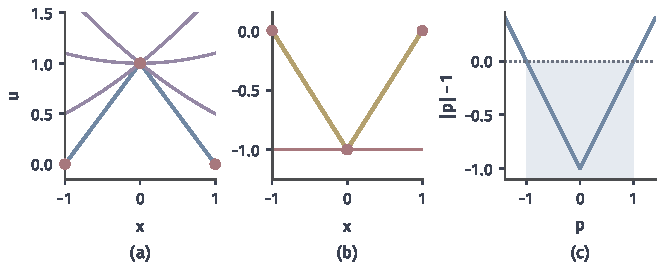
\includegraphics[width=112mm]{figures/06-differential-equations/02-partial-differential-equations/matplotlib/hj-kink-test/figure.pdf}
  \caption{程函方程$\lvert u'\rvert=1$（红点为边值）的折角检验。(a)$1-\lvert x\rvert$在顶点被紫线从上方贴住，斜率在$[-1,1]$内。(b)$\lvert x\rvert-1$在底点被水平红线从下方贴住，斜率$0$。(c)$\lvert p\rvert-1$，浅蓝范围内它不大于$0$：次解条件成立而上解条件不成立。}
  \label{fig:hj-kink-test}
\end{BookInlineFigure}

这个检验在到达时间问题中有直观的含义。若$T$在内部有凸折角，那么该点比它左右两边都早被到达，可是波前只能从相邻位置传来，内部没有源的地方不可能出现这种情况。凹折角则是两列波前相遇的地方，这是允许的。

定义对方程的符号敏感。把$F$换成$-F$，上下解的角色互换，方程$-\lvert u'\rvert+1=0$的黏性解是$\lvert x\rvert-1$，而不是$1-\lvert x\rvert$。这一点和弱解不同：弱形式乘$-1$不改变解集。这里的符号规定了信息传播的方向，$\partial_tu+H=0$中$\partial_tu$的系数为正，这是时间向前的方向。

对高维的到达时间问题，同样的两步检验可以直接做。

\begin{theorem}[距离函数]
\label{thm:hj-distance}
设$\Omega\subset\mathbb{R}^{d}$是开集，$\Omega\neq\mathbb{R}^{d}$，$u(\bm{x})$是$\bm{x}$到$\partial\Omega$的最短欧氏距离。则$u$是
\begin{equation}
  \lVert\nabla u\rVert_2-1=0\quad\text{在}\ \Omega\ \text{内}
  \label{eq:hj-distance}
\end{equation}
的黏性解。
\end{theorem}

\begin{proof}
三角不等式说明$u$是$1$-Lipschitz的。局部极大处，由引理~\ref{lem:hj-lipschitz-touch}得$\lVert\nabla\varphi\rVert_2\leq1$，次解条件成立。

设$u-\varphi$在$\bm{x}\in\Omega$取局部极小值，$\bm{y}\in\partial\Omega$是最近点，$\bm{e}$是从$\bm{x}$指向$\bm{y}$的单位向量。对小$h>0$，$\bm{x}_h=\bm{x}+h\bm{e}$仍在$\Omega$内，并且
\[
  u(\bm{x}_h)\leq\lVert\bm{x}_h-\bm{y}\rVert_2=u(\bm{x})-h.
\]
由局部极小，得到
\[
  \varphi(\bm{x}_h)-\varphi(\bm{x})\leq u(\bm{x}_h)-u(\bm{x})\leq-h.
\]
除以$h$并令$h\to0$，得到$\langle\nabla\varphi,\bm{e}\rangle\leq-1$，所以$\lVert\nabla\varphi(\bm{x})\rVert_2\geq1$，上解条件成立。
\end{proof}

取$\Omega=\mathbb{R}^2\setminus\{\bm{a},\bm{b}\}$，就知道图~\ref{fig:hj-two-sources}的$T=\min\{T_1,T_2\}$是黏性解。“第一次到达”这个物理选择，在方程层面就是黏性条件。

\paragraph{时间依赖的折角}
再回到凹槽$w$。它在$(0,t)$处的折角和$(t/2,t)$处的折角方向相反，检验结果也相反。

\begin{example}[凹槽不是黏性解]
\label{ex:hj-notch-test}
在$t_0>0$的点$(0,t_0)$附近，$w=\lvert x\rvert-t/2$。函数$\varphi=-t/2$从下方贴住$w$，其$q=\partial_t\varphi=-1/2$，$p=\partial_x\varphi=0$。上解条件要求
\[
  q+\frac{p^2}{2}=-\frac12\geq0,
\]
不成立，所以$w$不是上解。

对比$x=t/2$的折角。在那里$w=\min\{x-t/2,\ 0\}$，从上方贴住的测试函数，其$(q,p)$落在两个平面梯度$(-\tfrac12,1)$和$(0,0)$的连线上，写成$(q,p)=(-s/2,s)$，$0\leq s\leq1$。代入得到
\[
  q+\frac{p^2}{2}=-\frac{s}{2}+\frac{s^2}{2}\leq0,
\]
次解条件成立。这个折角是允许的。
\end{example}

图~\ref{fig:hj-notch-test}是这两个量。第一个折角对应$v$的左值小于右值的跳跃，第二个对应左值大于右值的跳跃，这和第~\ref{sec:hj-cusps}节由熵条件得到的判断一致。黏性解的定义不用导数，却自动区分了这两种跳跃。

\begin{BookInlineFigure}
  \centering
  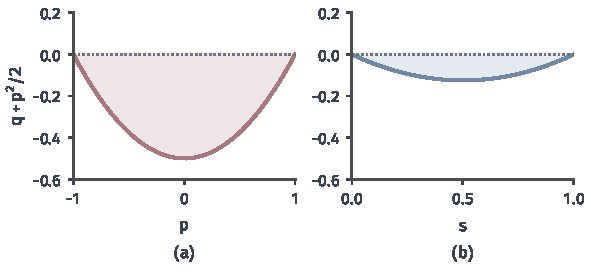
\includegraphics[width=100mm]{figures/06-differential-equations/02-partial-differential-equations/matplotlib/hj-notch-test/figure.pdf}
  \caption{凹槽$w$两类折角上的检验量$q+p^2/2$。(a)底部$x=0$处，$q=-1/2$，$\lvert p\rvert\leq1$，红线全部为负，上解条件不满足。(b)$x=t/2$处，$(q,p)=(-s/2,s)$，蓝线全部非正，次解条件满足。}
  \label{fig:hj-notch-test}
\end{BookInlineFigure}

\paragraph{与弱解的区别}
黏性解和弱解都用测试函数，但做的事情不一样。弱解把方程乘上测试函数积分，导数通过分部积分转到测试函数上，方程必须有散度形式。黏性解不做积分，也不移走导数，它只在测试函数贴住解的一点上读取一阶导数，建立一个微分不等式。表~\ref{tab:hj-weak-vs-viscosity}把两者并列。

\begin{BookInlineTable}
  \centering
  \begin{tabular}{lll}
    \toprule
    & 弱解 & 黏性解\\
    \midrule
    测试函数的角色 & 乘上去做积分 & 在接触点处提供导数\\
    检验位置 & 整个区域的积分 & 逐点的不等式\\
    需要的结构 & 散度形式 & 方程的符号（单调性）\\
    方程乘$-1$ & 解不变 & 解改变\\
    对极限的稳定性 & 弱收敛下通量要可控 & 局部一致收敛即可\\
    \bottomrule
  \end{tabular}
  \caption{弱解与黏性解的对比。}
  \label{tab:hj-weak-vs-viscosity}
\end{BookInlineTable}

所以黏性解并不是把方程积分一下得到的弱化形式，$H(\nabla u)$非线性时，分部积分本来就做不了。这个定义的价值要由下一节的比较原理来兑现。

\section{比较原理}
\label{sec:hj-comparison}

黏性解的定义只是几条不等式，它能确定唯一的函数吗？在到达时间的语言里，答案应当由一个朴素的事实决定：更早点燃的波前不会更晚到达。把它写成数学就是比较原理：次解在初始或边界上不超过上解，就处处不超过上解。

\paragraph{光滑情形的机制}
先看$u$、$v$都光滑的情形，$u$是次解，$v$是上解，$u(\cdot,0)\leq v(\cdot,0)$。假设$u-v$在某处为正，为了简单，设最大值在$t_0>0$的某点$(\bm{x}_0,t_0)$取到。在这一点
\[
  \nabla u=\nabla v,\qquad\partial_tu\geq\partial_tv,
\]
后一个不等号是因为最大值的时刻可能是右端点。两个方程相减，两个$H$在同一个梯度上取值，相互抵消，得到$\partial_tu-\partial_tv\leq0$。

这还不是矛盾，$\partial_tu=\partial_tv$是可能的。修补的办法是减去一个严格增长的时间函数，例如$\lambda t$或$\lambda/(t_{\mathrm{f}}-t)$，使极大点处的时间导数严格大于零，这样就矛盾了。

对只连续的$u$、$v$，上面的第一式无法写出：在$u-v$的极大点，$u$和$v$都可能不可微。解决办法是\term{变量倍增}（doubling of variables）：用两组独立的变量分别处理$u$和$v$，并加上惩罚项迫使它们靠近，
\[
  \Phi(\bm{x},\bm{y})=u(\bm{x})-v(\bm{y})-\frac{\lVert\bm{x}-\bm{y}\rVert_2^2}{\delta^2}.
\]

固定$\bm{y}$时，$\Phi$是$u$减去一个光滑函数，这个光滑函数可以作为$u$的测试函数；固定$\bm{x}$时同样能作为$v$的测试函数。两个测试函数的梯度都是$2(\bm{x}-\bm{y})/\delta^2$，同一个$\bm{p}$出现在两边，这正是光滑情形下$\nabla u=\nabla v$的替身。

图~\ref{fig:hj-doubling}用一对带折角的函数演示。$\delta$变小时，$\Phi$的正值区域被压向对角线，极大点（绿）也靠向对角线，且其高度趋向$u-v$的最大值。

\begin{BookInlineFigure}
  \centering
  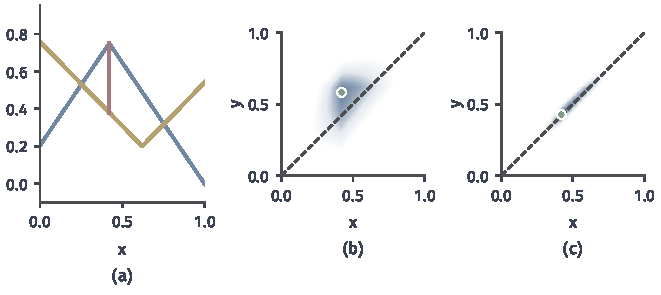
\includegraphics[width=112mm]{figures/06-differential-equations/02-partial-differential-equations/matplotlib/hj-doubling/figure.pdf}
  \caption{变量倍增。(a)$u$（蓝，凹折角）和$v$（黄，凸折角），红线段标出$u-v$的最大值。(b)、(c)$\Phi(x,y)$的正值，白色表示$\Phi\leq0$，蓝色越深值越大，绿点是极大点，虚线是对角线，$\delta=0.6$和$0.12$。}
  \label{fig:hj-doubling}
\end{BookInlineFigure}

\paragraph{初值问题}
下面是初值问题的比较原理。为了涵盖$H=p^2/2$这种关于$\bm{p}$不全局Lipschitz的情形，我们要求函数关于$\bm{x}$是Lipschitz的，这样只需要$H$在有界的$\bm{p}$上的性质。

\begin{theorem}[初值问题的比较原理]
\label{thm:hj-comparison}
设$H(t,\bm{x},\bm{p})$在$\lVert\bm{p}\rVert_2\leq R$的范围内关于全部自变量一致连续。设$u,v$在$\mathbb{R}^{d}\times[0,t_{\mathrm{f}}]$上有界、一致连续，关于$\bm{x}$是$R$-Lipschitz的，$u$是次解，$v$是上解。若$u(\cdot,0)\leq v(\cdot,0)$，则
\begin{equation}
  u\leq v\quad\text{在}\ \mathbb{R}^{d}\times[0,t_{\mathrm{f}}]\ \text{上}.
  \label{eq:hj-comparison}
\end{equation}
\end{theorem}

\begin{proof}
反设$\sigma=\sup(u-v)>0$。由连续性，存在$(\bar{\bm{x}},\bar{t})$，$\bar{t}<t_{\mathrm{f}}$，使$(u-v)(\bar{\bm{x}},\bar{t})>3\sigma/4$。对$\lambda,\delta>0$，记$\psi(t)=\lambda/(t_{\mathrm{f}}-t)$，并令
\[
  \begin{aligned}
    \Phi(\bm{x},\bm{y},t,s)={}&u(\bm{x},t)-v(\bm{y},s)-\psi(t)-\psi(s)\\
    &-\frac{\lVert\bm{x}-\bm{y}\rVert_2^2+(t-s)^2}{\delta^2}-\delta\bigl(\lVert\bm{x}\rVert_2^2+\lVert\bm{y}\rVert_2^2\bigr).
  \end{aligned}
\]
$\psi$在$t\to t_{\mathrm{f}}$时趋于无穷，二次项在无穷远处趋于负无穷，而$u,v$有界，所以$\Phi$在某点$(\bm{x}_0,\bm{y}_0,t_0,s_0)$取到最大值，且$t_0,s_0<t_{\mathrm{f}}$。先取$\lambda$充分小，此后只令$\delta\to0$，使得
\[
  \Phi(\bm{x}_0,\bm{y}_0,t_0,s_0)\geq\Phi(\bar{\bm{x}},\bar{\bm{x}},\bar{t},\bar{t})\geq\frac{\sigma}{2}.
\]

第一步估计最大点。记$C_0=\sup\lvert u\rvert+\sup\lvert v\rvert$。由上式，各惩罚项之和不超过$u(\bm{x}_0,t_0)-v(\bm{y}_0,s_0)\leq C_0$，所以
\[
  \begin{gathered}
    \lVert\bm{x}_0-\bm{y}_0\rVert_2\leq\sqrt{C_0}\,\delta,\qquad\lvert t_0-s_0\rvert\leq\sqrt{C_0}\,\delta,\\
    \delta\lVert\bm{x}_0\rVert_2\leq\sqrt{C_0\delta},\qquad\delta\lVert\bm{y}_0\rVert_2\leq\sqrt{C_0\delta}.
  \end{gathered}
\]

第二步说明$t_0,s_0>0$。若$t_0=0$，由$u(\cdot,0)\leq v(\cdot,0)$，
\[
  \frac{\sigma}{2}\leq u(\bm{x}_0,0)-v(\bm{y}_0,s_0)\leq v(\bm{x}_0,0)-v(\bm{y}_0,s_0).
\]
$s_0=\lvert t_0-s_0\rvert$，右端在$\delta\to0$时由$v$的一致连续性趋于零，矛盾。若$s_0=0$，同样用$u$的一致连续性得到矛盾。

第三步使用次解和上解的定义。记$\bm{p}=2(\bm{x}_0-\bm{y}_0)/\delta^2$。固定$(\bm{y}_0,s_0)$，函数$(\bm{x},t)\mapsto\Phi$是$u$减去$C^1$函数，它在$(\bm{x}_0,t_0)$取极大。测试函数的时间导数是$\psi'(t_0)+2(t_0-s_0)/\delta^2$，梯度是$\bm{p}+2\delta\bm{x}_0$，所以由次解条件，
\[
  \psi'(t_0)+\frac{2(t_0-s_0)}{\delta^2}+H\bigl(t_0,\bm{x}_0,\bm{p}+2\delta\bm{x}_0\bigr)\leq0.
\]

固定$(\bm{x}_0,t_0)$，$v$减去相应的$C^1$函数在$(\bm{y}_0,s_0)$取极小，测试函数的时间导数是$-\psi'(s_0)+2(t_0-s_0)/\delta^2$，梯度是$\bm{p}-2\delta\bm{y}_0$。由上解条件，
\[
  -\psi'(s_0)+\frac{2(t_0-s_0)}{\delta^2}+H\bigl(s_0,\bm{y}_0,\bm{p}-2\delta\bm{y}_0\bigr)\geq0.
\]

两式相减，$2(t_0-s_0)/\delta^2$抵消，得到
\[
  \psi'(t_0)+\psi'(s_0)\leq H\bigl(s_0,\bm{y}_0,\bm{p}-2\delta\bm{y}_0\bigr)-H\bigl(t_0,\bm{x}_0,\bm{p}+2\delta\bm{x}_0\bigr).
\]
由引理~\ref{lem:hj-lipschitz-touch}，两个梯度的长度都不超过$R$，所以可以用$H$的一致连续性。两组自变量的距离由第一步趋于零，右端趋于零。

而左端不小于$2\lambda/t_{\mathrm{f}}^2$，是一个与$\delta$无关的正数，矛盾。
\end{proof}

证明中每个假设的作用都能指出来。有界性让$\delta\lVert\bm{x}\rVert_2^2$这一项能把最大点留在有限范围内，这是增长条件的来源。一致连续性让第二步能把最大点推离$t=0$。Lipschitz条件和$H$的一致连续性负责最后一步。$\psi$的引入提供了严格的正数。

比较原理立刻给出唯一性和连续依赖。

\begin{theorem}[唯一性与数据稳定性]
\label{thm:hj-uniqueness}
在定理~\ref{thm:hj-comparison}的条件下，设$u$、$v$是黏性解，初值分别为$u_0$、$v_0$，$H$不依赖场值。则对$0\leq t\leq t_{\mathrm{f}}$，
\begin{equation}
  \sup_{\bm{x}}\lvert u(\bm{x},t)-v(\bm{x},t)\rvert\leq\sup_{\bm{x}}\lvert u_0(\bm{x})-v_0(\bm{x})\rvert.
  \label{eq:hj-stability}
\end{equation}
特别地，在这一函数类中，同一初值的黏性解至多一个。
\end{theorem}

\begin{proof}
记$K=\sup\lvert u_0-v_0\rvert$。$H$不依赖场值，所以$v+K$仍是黏性解，因为加常数不改变测试函数的导数。此时$u_0\leq v_0+K$，由比较原理得$u\leq v+K$。交换$u$、$v$得到另一半。$K=0$时就是唯一性。
\end{proof}

式~\eqref{eq:hj-stability}说明，解到解的映射在上确界范数下不扩张。图~\ref{fig:hj-order-preserved}用第~\ref{sec:hj-hopf-lax}节的公式算了一个例子：初值的差在$[0,0.6]$内，此后$u\leq v$一直保持，差的最大值始终不超过$0.6$，差的最小值保持为$0$。

\begin{BookInlineFigure}
  \centering
  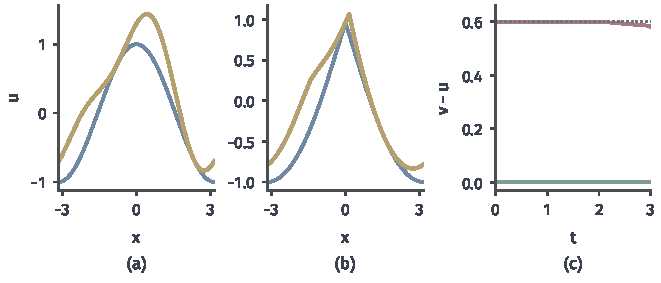
\includegraphics[width=112mm]{figures/06-differential-equations/02-partial-differential-equations/matplotlib/hj-order-preserved/figure.pdf}
  \caption{次序保持与上确界稳定性，$H=p^2/2$。(a)初值$u_0=\cos x$（蓝）和$v_0=\cos x+0.3+0.3\sin2x$（黄），$v_0\geq u_0$。(b)$t=1.2$的解，次序不变。(c)$v-u$的最大值（红）和最小值（绿）随时间的变化，虚线是初始最大差$0.6$。}
  \label{fig:hj-order-preserved}
\end{BookInlineFigure}

比较原理还给出简单的先验界。对$H=p^2/2$和例~\ref{ex:hj-cos}，常数$\pm1$都是经典解，$-1\leq\cos x\leq1$，所以在所有时刻$-1\leq u\leq1$。不解方程就知道了解的范围。

也可以用它解释凹槽为什么被排除。若$w$是上解，将它和次解$0$比较，初值都是$0$，比较原理给出$0\leq w$，而$w$在凹槽内为负。所以$w$不可能是上解，这就是例~\ref{ex:hj-notch-test}在底部折角处看到的失败。整体的比较结论，靠的正是接触点处的不等式。

条件不能随意去掉。取无界的初值$u_0=-x^2/2$，$H=p^2/2$，由特征线得到经典解
\[
  u(x,t)=-\frac{x^2}{2(1-t)},\qquad0\leq t<1.
\]
当$t\uparrow1$时，$u(x,t)\to-\infty$（$x\neq0$），没有办法延拓到$t\geq1$。有界性假设排除的就是这种从无穷远处传来的影响。

\paragraph{边值问题}
稳态的到达时间问题没有时间方向，上面证明中的$\psi$无从谈起，严格性要用别的办法得到。程函方程里可以把次解乘一个小于$1$的常数。

\begin{theorem}[程函方程的比较原理]
\label{thm:hj-comparison-eikonal}
设$\Omega\subset\mathbb{R}^{d}$有界开，$n\in C(\overline{\Omega})$，$n>0$。设$u,v\in C(\overline{\Omega})$分别是$\lVert\nabla u\rVert_2=n$在$\Omega$内的次解和上解，并且在$\partial\Omega$上$u\leq v$，则
\begin{equation}
  u\leq v\quad\text{在}\ \overline{\Omega}\ \text{上}.
  \label{eq:hj-comparison-eikonal}
\end{equation}
\end{theorem}

\begin{proof}
反设$\sigma=\max_{\overline{\Omega}}(u-v)>0$。取$\theta\in(0,1)$充分接近$1$，使$(1-\theta)\max\lvert u\rvert<\sigma/4$，于是$\sigma'=\max(\theta u-v)\geq3\sigma/4$，而在$\partial\Omega$上$\theta u-v\leq\sigma/4$。

对$\delta>0$，令
\[
  \Phi(\bm{x},\bm{y})=\theta u(\bm{x})-v(\bm{y})-\frac{\lVert\bm{x}-\bm{y}\rVert_2^2}{\delta^2},
\]
它在紧集$\overline{\Omega}\times\overline{\Omega}$上的最大点记为$(\bm{x}_\delta,\bm{y}_\delta)$。$\Phi$的最大值不小于$\sigma'$，所以惩罚项有界，$\lVert\bm{x}_\delta-\bm{y}_\delta\rVert_2\to0$。取子列使$\bm{x}_\delta,\bm{y}_\delta\to\bm{z}$，由连续性
\[
  \theta u(\bm{z})-v(\bm{z})\geq\sigma'\geq\frac{3\sigma}{4}.
\]
这说明$\bm{z}\notin\partial\Omega$，$\delta$小时$\bm{x}_\delta,\bm{y}_\delta$都在$\Omega$内。

记$\bm{p}=2(\bm{x}_\delta-\bm{y}_\delta)/\delta^2$。固定$\bm{y}_\delta$，$u$减去光滑函数在$\bm{x}_\delta$取极大，测试函数的梯度是$\bm{p}/\theta$，由次解条件$\lVert\bm{p}\rVert_2/\theta\leq n(\bm{x}_\delta)$。固定$\bm{x}_\delta$，由上解条件$\lVert\bm{p}\rVert_2\geq n(\bm{y}_\delta)$。两式合并，得到
\[
  n(\bm{y}_\delta)\leq\theta\,n(\bm{x}_\delta).
\]
令$\delta\to0$，$n(\bm{z})\leq\theta n(\bm{z})$，与$n(\bm{z})>0$、$\theta<1$矛盾。
\end{proof}

取$n=1/c$，$c$连续且有正的上下界，这个定理就适用于第~\ref{sec:hj-problem}节的到达时间问题，方程写成$c\lVert\nabla T\rVert_2-1=0$和$\lVert\nabla T\rVert_2-n=0$时次解、上解的条件相同，因为$c>0$不改变不等号方向。定理~\ref{thm:hj-distance}的距离函数在有界区域上是边值为零的唯一黏性解。

正性$n>0$的作用是提供严格性。若$n$在某点为零，可以看到比较原理失败。在$(-1,1)$上取$\lvert u'\rvert=2\lvert x\rvert$，$u(\pm1)=0$，这里$n(0)=0$，相当于速度在原点为无穷大。则
\[
  u=1-x^2\qquad\text{和}\qquad u=x^2-1
\]
都是$C^1$的经典解，因而都是黏性解，见图~\ref{fig:hj-boundary-failures}(a)。这就破坏了唯一性。

\begin{BookInlineFigure}
  \centering
  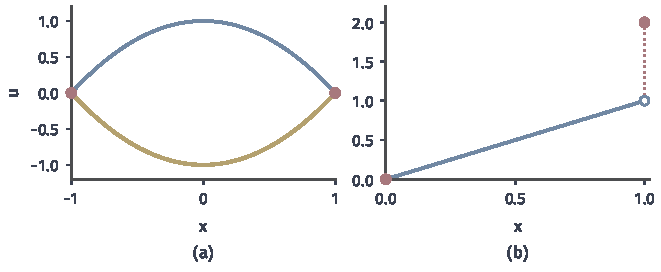
\includegraphics[width=112mm]{figures/06-differential-equations/02-partial-differential-equations/matplotlib/hj-boundary-failures/figure.pdf}
  \caption{边值问题的两种失败。(a)$\lvert u'\rvert=2\lvert x\rvert$，$u(\pm1)=0$（红点）有两个经典解$1-x^2$（蓝）和$x^2-1$（黄）。(b)$\lvert u'\rvert=1$，$u(0)=0$，$u(1)=2$（红点）：连续解取$u=x$，在右端得到$u(1)=1$（空心点），边值$2$没有被达到。}
  \label{fig:hj-boundary-failures}
\end{BookInlineFigure}

边界数据不相容时，问题出在另一处。在$(0,1)$上取$\lvert u'\rvert=1$，$u(0)=0$，$u(1)=2$。方程要求$u$是$1$-Lipschitz的，$u(1)$不可能等于$2$。自然的候选是
\[
  u(x)=\min\{0+x,\ 2+(1-x)\}=x,
\]
它在$(0,1)$内是黏性解，但在右端取值$1$，边值$2$被丢掉了，见图~\ref{fig:hj-boundary-failures}(b)。这对应第~\ref{sec:hj-problem}节的相容性条件。边值问题的比较原理假定函数已经在边界上按要求比较，它并不保证任何数据都能取到。

初值问题不会出现边值丢失，这里的差别列在表~\ref{tab:hj-comparison-cases}中，一种情形的结论不能搬到另一种情形。

\begin{BookInlineTable}
  \centering
  \begin{tabular}{lll}
    \toprule
    & 初值问题 & 程函边值问题\\
    \midrule
    严格性来源 & 时间函数$\psi$ & 系数$\theta<1$与$n>0$\\
    比较的部位 & $t=0$，全空间 & 边界$\partial\Omega$\\
    无穷远的控制 & 有界性、$\delta\lVert\bm{x}\rVert_2^2$ & 有界区域\\
    数据的限制 & 有界且Lipschitz & 需要相容，否则边值丢失\\
    条件破坏时 & 爆破、非唯一 & $n$有零点时非唯一\\
    \bottomrule
  \end{tabular}
  \caption{初值问题与边值问题的比较原理。}
  \label{tab:hj-comparison-cases}
\end{BookInlineTable}

\section{Hopf--Lax表示}
\label{sec:hj-hopf-lax}

比较原理保证黏性解至多一个，存在性还没有解决。对只依赖梯度的凸Hamilton量，解可以显式写出来，而且公式直接解释了尖点处选了哪一支。

\paragraph{从特征线到极小化}
设$H=H(\bm{p})$是凸函数，并且\term{超线性增长}（superlinear growth），即
\begin{equation}
  \lim_{\lVert\bm{p}\rVert_2\to\infty}\frac{H(\bm{p})}{\lVert\bm{p}\rVert_2}=+\infty.
  \label{eq:hj-superlinear}
\end{equation}
由第~\ref{sec:hj-characteristics}节的特征方程组，特征线是直线，斜率$\bm{p}$不变，速度$\bm{q}=\nabla H(\bm{p})$。沿线值的增量$\langle\bm{p},\nabla H(\bm{p})\rangle-H(\bm{p})$可以只用$\bm{q}$表示。

这里要用到凸共轭：对凸函数$H$，定义
\begin{equation}
  L(\bm{q})=\sup_{\bm{p}\in\mathbb{R}^{d}}\bigl\{\langle\bm{p},\bm{q}\rangle-H(\bm{p})\bigr\}.
  \label{eq:hj-legendre}
\end{equation}
$H$在$\bm{p}$处可微且$\bm{q}=\nabla H(\bm{p})$时，上确界在$\bm{p}$处取到，因此$L(\bm{q})=\langle\bm{p},\bm{q}\rangle-H(\bm{p})$，恰好是沿特征线值的增长率。凸共轭的基本性质（下半连续的凸函数共轭两次回到自身）可参考\BookChapterRef{chap:duality}{卷五第18章“对偶问题”}。

超线性让事情变得简单。对任意$r>0$，取$\bm{p}=r\bm{q}/\lVert\bm{q}\rVert_2$代入式~\eqref{eq:hj-legendre}，得到
\[
  L(\bm{q})\geq r\lVert\bm{q}\rVert_2-\max_{\lVert\bm{p}\rVert_2=r}H(\bm{p}).
\]
所以$L$同样超线性增长；由式~\eqref{eq:hj-superlinear}，式~\eqref{eq:hj-legendre}中的上确界有限。$L$是有限的凸函数，因而连续，并且由Fenchel--Moreau定理$H=L^*$。

最常用的例子是$H(\bm{p})=\lVert\bm{p}\rVert_2^2/2$，它的共轭是$L(\bm{q})=\lVert\bm{q}\rVert_2^2/2$。

从$\bm{y}$出发、时间$t$内到达$\bm{x}$的特征线速度是$\bm{q}=(\bm{x}-\bm{y})/t$，所以它带来的值是$u_0(\bm{y})+tL(\bm{q})$。不同的$\bm{y}$给出不同的候选值，我们取最小的一个。

\begin{definition}[Hopf--Lax公式]
\label{def:hj-hopf-lax}
设$H$凸且超线性增长，$L=H^*$，$u_0$有界且$R$-Lipschitz。对$t>0$，定义
\begin{equation}
  u(\bm{x},t)=\min_{\bm{y}\in\mathbb{R}^{d}}\Bigl\{u_0(\bm{y})+tL\Bigl(\frac{\bm{x}-\bm{y}}{t}\Bigr)\Bigr\},
  \label{eq:hj-hopf-lax}
\end{equation}
并令$u(\cdot,0)=u_0$。式~\eqref{eq:hj-hopf-lax}称为\term{Hopf--Lax公式}（Hopf--Lax formula）。
\end{definition}

对$H=p^2/2$，公式写成
\[
  u(x,t)=\min_y\Bigl\{u_0(y)+\frac{(x-y)^2}{2t}\Bigr\}.
\]
它有一个直观的图景，见图~\ref{fig:hj-parabola-touch}。把开口向下、顶点在$(x,c)$的抛物线$c-(x-y)^2/(2t)$放在$u_0$的下方，向上抬，直到碰到$u_0$，此时的$c$就是$u(x,t)$。接触点$y$是极小点，也就是这个位置的解“来自”的初始点。

\begin{BookInlineFigure}
  \centering
  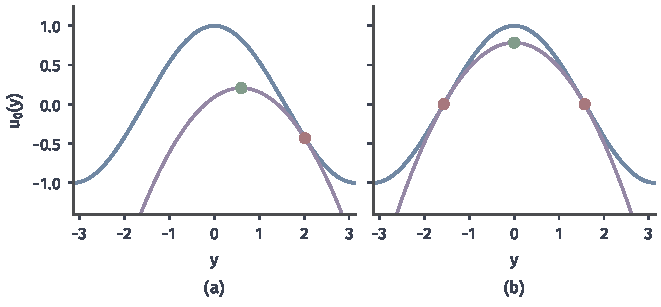
\includegraphics[width=112mm]{figures/06-differential-equations/02-partial-differential-equations/matplotlib/hj-parabola-touch/figure.pdf}
  \caption{Hopf--Lax公式的抛物线图景，$u_0=\cos y$（蓝），$t=\pi/2$。紫线是抬到碰上$u_0$为止的抛物线，绿点是顶点$(x,u(x,t))$，红点是接触点。(a)$x=0.6$，只有一个接触点。(b)$x=0$，两个接触点$y=\pm\pi/2$，顶点高度$\pi/4$。}
  \label{fig:hj-parabola-touch}
\end{BookInlineFigure}

\paragraph{公式的性质}
要证明式~\eqref{eq:hj-hopf-lax}给出黏性解，需要它的四条性质。最关键的一条是半群性质：走$t$时间等于先走$s$，再走$t-s$。

\begin{lemma}[Hopf--Lax公式的性质]
\label{lem:hj-hopf-lax}
在定义~\ref{def:hj-hopf-lax}的条件下：

(1)式~\eqref{eq:hj-hopf-lax}的极小值可以取到。

(2)$u(\cdot,t)$是$R$-Lipschitz的。

(3)对$0\leq s<t$，
\begin{equation}
  u(\bm{x},t)=\min_{\bm{y}}\Bigl\{u(\bm{y},s)+(t-s)L\Bigl(\frac{\bm{x}-\bm{y}}{t-s}\Bigr)\Bigr\}.
  \label{eq:hj-semigroup}
\end{equation}

(4)记
\begin{equation}
  C=\max\Bigl\{\lvert L(\bm{0})\rvert,\ \max_{\lVert\bm{p}\rVert_2\leq R}\lvert H(\bm{p})\rvert\Bigr\},
  \label{eq:hj-time-constant}
\end{equation}
则对$0\leq s\leq t$，
\begin{equation}
  \lvert u(\bm{x},t)-u(\bm{x},s)\rvert\leq C(t-s).
  \label{eq:hj-time-lipschitz}
\end{equation}
\end{lemma}

\begin{proof}
(1)括号内是$\bm{y}$的连续函数。$u_0$有界，$L$超线性增长，所以当$\lVert\bm{y}\rVert_2\to\infty$时括号内趋于$+\infty$，极小值可取到。

(2)设$\bm{y}$是$(\bm{x},t)$的极小点。把$\bm{y}+\hat{\bm{x}}-\bm{x}$代入$(\hat{\bm{x}},t)$的公式，$L$的自变量不变，所以
\[
  u(\hat{\bm{x}},t)-u(\bm{x},t)\leq u_0(\bm{y}+\hat{\bm{x}}-\bm{x})-u_0(\bm{y})\leq R\lVert\hat{\bm{x}}-\bm{x}\rVert_2.
\]
交换$\bm{x}$和$\hat{\bm{x}}$得到另一半。

(3)$s=0$时就是定义。设$s>0$。先证式中右端不超过左端。设$\bm{z}$是$(\bm{x},t)$的极小点，取线段上的点$\bm{y}=\frac{s}{t}\bm{x}+(1-\frac{s}{t})\bm{z}$，此时
\[
  \frac{\bm{x}-\bm{y}}{t-s}=\frac{\bm{y}-\bm{z}}{s}=\frac{\bm{x}-\bm{z}}{t}.
\]
用$u(\bm{y},s)\leq u_0(\bm{z})+sL((\bm{y}-\bm{z})/s)$，右端括号内不超过$u_0(\bm{z})+tL((\bm{x}-\bm{z})/t)=u(\bm{x},t)$。

再证左端不超过右端。任取$\bm{y}$，设$\bm{z}$是$(\bm{y},s)$的极小点。由$L$的凸性，
\[
  tL\Bigl(\frac{\bm{x}-\bm{z}}{t}\Bigr)\leq(t-s)L\Bigl(\frac{\bm{x}-\bm{y}}{t-s}\Bigr)+sL\Bigl(\frac{\bm{y}-\bm{z}}{s}\Bigr).
\]
再由$u(\bm{x},t)$的定义，得到
\[
  u(\bm{x},t)\leq u_0(\bm{z})+tL\Bigl(\frac{\bm{x}-\bm{z}}{t}\Bigr)\leq u(\bm{y},s)+(t-s)L\Bigl(\frac{\bm{x}-\bm{y}}{t-s}\Bigr).
\]

(4)先证$s=0$。上界由$\bm{y}=\bm{x}$得到：$u(\bm{x},t)\leq u_0(\bm{x})+tL(\bm{0})$。下界用$\bm{z}=(\bm{x}-\bm{y})/t$改写公式，再用Lipschitz条件：
\[
  u(\bm{x},t)\geq u_0(\bm{x})+t\min_{\bm{z}}\bigl\{L(\bm{z})-R\lVert\bm{z}\rVert_2\bigr\}.
\]
而$R\lVert\bm{z}\rVert_2$等于$\langle\bm{p},\bm{z}\rangle$在$\lVert\bm{p}\rVert_2\leq R$上的最大值。交换两个$\max$并用$H=L^*$，得到
\[
  -\min_{\bm{z}}\bigl\{L(\bm{z})-R\lVert\bm{z}\rVert_2\bigr\}=\max_{\lVert\bm{p}\rVert_2\leq R}H(\bm{p})\leq C.
\]
一般的$s$由式~\eqref{eq:hj-semigroup}和(2)，把$u(\cdot,s)$当作新的初值重复这一论证。
\end{proof}

\begin{theorem}[Hopf--Lax公式给出黏性解]
\label{thm:hj-hopf-lax}
在定义~\ref{def:hj-hopf-lax}的条件下，式~\eqref{eq:hj-hopf-lax}定义的$u$在任意$\mathbb{R}^{d}\times[0,t_{\mathrm{f}}]$上有界、Lipschitz，是初值问题$\partial_tu+H(\nabla u)=0$、$u(\cdot,0)=u_0$的黏性解，并且是有界、一致连续、关于$\bm{x}$为$R$-Lipschitz的函数类中唯一的黏性解。
\end{theorem}

\begin{proof}
由引理~\ref{lem:hj-hopf-lax}，$u$有界，界为$\sup\lvert u_0\rvert+Ct_{\mathrm{f}}$；$u$关于$\bm{x}$是$R$-Lipschitz的，关于$t$是$C$-Lipschitz的，$t=0$时取值$u_0$。

\emph{次解。}设$u-\varphi$在$(\bm{x}_0,t_0)$取局部极大，$t_0>0$。任取$\bm{q}$和小$h>0$，在式~\eqref{eq:hj-semigroup}中取$\bm{y}=\bm{x}_0-h\bm{q}$、$s=t_0-h$，得到
\[
  u(\bm{x}_0,t_0)\leq u(\bm{x}_0-h\bm{q},t_0-h)+hL(\bm{q}).
\]
由局部极大，$u-\varphi$在$(\bm{x}_0-h\bm{q},t_0-h)$处不大于在$(\bm{x}_0,t_0)$处，整理后得到
\[
  \varphi(\bm{x}_0,t_0)-\varphi(\bm{x}_0-h\bm{q},t_0-h)\leq hL(\bm{q}).
\]
除以$h$，令$h\to0$，得到
\[
  \partial_t\varphi+\langle\bm{q},\nabla\varphi\rangle-L(\bm{q})\leq0.
\]
对$\bm{q}$取上确界并用$H=L^*$，得到$\partial_t\varphi+H(\nabla\varphi)\leq0$。

\emph{上解。}设$u-\varphi$在$(\bm{x}_0,t_0)$取局部极小。由式~\eqref{eq:hj-semigroup}（取$s=t_0-h$）和(1)，存在$\bm{y}_h$，记$\bm{q}_h=(\bm{x}_0-\bm{y}_h)/h$，使
\[
  u(\bm{x}_0,t_0)=u(\bm{y}_h,t_0-h)+hL(\bm{q}_h).
\]
由$u$的Lipschitz性质，$hL(\bm{q}_h)\leq Rh\lVert\bm{q}_h\rVert_2+Ch$。$L$超线性增长，所以$\lVert\bm{q}_h\rVert_2$有不依赖$h$的上界。

由局部极小，同样整理得到
\[
  \varphi(\bm{x}_0,t_0)-\varphi(\bm{y}_h,t_0-h)\geq hL(\bm{q}_h).
\]
$\varphi\in C^1$且$\bm{q}_h$有界，所以左端等于$h(\partial_t\varphi+\langle\bm{q}_h,\nabla\varphi\rangle)+o(h)$，其中导数在$(\bm{x}_0,t_0)$处取值。除以$h$，得到
\[
  \partial_t\varphi+\langle\bm{q}_h,\nabla\varphi\rangle-L(\bm{q}_h)\geq o(1).
\]
由Fenchel--Young不等式（$H=L^*$的定义），左端第二、三两项不超过$H(\nabla\varphi)$。令$h\to0$，得到$\partial_t\varphi+H(\nabla\varphi)\geq0$。

\emph{唯一性。}$H$连续，在$\lVert\bm{p}\rVert_2\leq R$上一致连续，由定理~\ref{thm:hj-uniqueness}即得。
\end{proof}

证明的结构和方程的含义一一对应：极小化的上界对应每一条候选路线都给出不等式，所以次解成立；极小化取到的那条路线给出反向的不等式，所以上解成立。

\paragraph{公式怎样选择分支}
回到$u_0=\cos x$，取$t=\pi/2$、$x=0$。极小化的函数是$F(y)=\cos y+y^2/\pi$，临界点方程是
\[
  F'(y)=-\sin y+\frac{2y}{\pi}=0,
\]
即$\sin y=2y/\pi$。由$\sin$在$[0,\pi]$上的凹性，它的非负解只有$y=0$和$y=\pi/2$；再由对称性，全部解是$y=0,\pm\pi/2$。代入$F$得到
\[
  F(0)=1,\qquad F\bigl(\pm\tfrac{\pi}{2}\bigr)=\frac{\pi}{4}\approx0.785.
\]
所以$u(0,\pi/2)=\pi/4$，极小点是$y=\pm\pi/2$。这三个临界点恰好是第~\ref{sec:hj-cusps}节算出的三条特征线，函数值也与当时的$z$相同。

这个吻合有一般的原因。设$u_0$、$L$、$H$可微，$\bm{q}$表示$(\bm{x}-\bm{y})/t$，极小点满足一阶条件$\nabla u_0(\bm{y})=\nabla L(\bm{q})$。由共轭函数的性质，这等价于$\bm{q}$等于$\nabla H$在$\bm{p}_0=\nabla u_0(\bm{y})$处的值，也就是
\[
  \bm{x}=\bm{y}+t\nabla H(\bm{p}_0).
\]
所以每个临界点都对应一条到达$(\bm{x},t)$的特征线，临界值就是这条线带来的$z$。Hopf--Lax公式在所有特征线中选择取值最小的一条，这回答了第~\ref{sec:hj-cusps}节的问题：对凸的$H$，黏性解取的就是所有特征线候选的下包络。

图~\ref{fig:hj-argmin-jump}(a)是目标函数$F$。$x=0$时两个极小点等高；$x=0.3$时右侧变低，唯一的极小点约为$y=1.822$，极小值$0.489$。图(b)是极小点随$x$的变化，在$x=0$处从$-\pi/2$跳到$\pi/2$，这个跳跃就是图~\ref{fig:hj-cos-characteristics}(b)中两族特征线之间的分界。

\begin{BookInlineFigure}
  \centering
  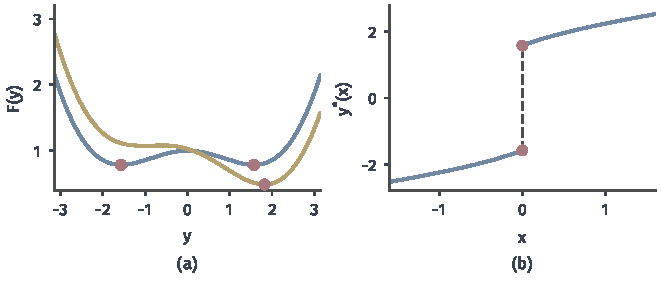
\includegraphics[width=112mm]{figures/06-differential-equations/02-partial-differential-equations/matplotlib/hj-argmin-jump/figure.pdf}
  \caption{极小点的跳跃，$t=\pi/2$，$F(y)=\cos y+(x-y)^2/(2t)$。(a)$x=0$（蓝）有两个等高的极小点，$x=0.3$（黄）只有一个，红点是极小点。(b)极小点$y^*(x)$，虚线处从$-\pi/2$跳到$\pi/2$。}
  \label{fig:hj-argmin-jump}
\end{BookInlineFigure}

\begin{theorem}[极小点决定梯度]
\label{thm:hj-minimizer-gradient}
设$L$连续可微，$\bm{y}$是$(\bm{x},t)$的一个极小点，$t>0$。若$u(\cdot,t)$在$\bm{x}$处可微，则
\begin{equation}
  \nabla u(\bm{x},t)=\nabla L\Bigl(\frac{\bm{x}-\bm{y}}{t}\Bigr).
  \label{eq:hj-minimizer-gradient}
\end{equation}
特别地，若$L$还是严格凸的，而$(\bm{x},t)$有两个不同的极小点，则$u(\cdot,t)$在$\bm{x}$处不可微。
\end{theorem}

\begin{proof}
对任意$\bm{x}'$，$\bm{y}$仍是公式的一个候选，所以
\[
  u(\bm{x}',t)\leq u_0(\bm{y})+tL\Bigl(\frac{\bm{x}'-\bm{y}}{t}\Bigr),
\]
且$\bm{x}'=\bm{x}$时取等。右端是$\bm{x}'$的$C^1$函数，从上方贴住$u(\cdot,t)$，一阶条件给出式~\eqref{eq:hj-minimizer-gradient}。

若有两个极小点，$(\bm{x}-\bm{y})/t$取两个不同的值，严格凸函数的梯度是单射，式~\eqref{eq:hj-minimizer-gradient}的右端不同，矛盾。
\end{proof}

不可微点就是多个极小点的位置，也就是特征线竞争时打平的位置。在$x=0$、$t=\pi/2$，两个极小点给出$q=(0\mp\pi/2)/(\pi/2)=\mp1$，$u$的左斜率是$+1$，右斜率是$-1$，形成凹折角。

折角只会是凹的，这一点可以直接证明。对$H=\lVert\bm{p}\rVert_2^2/2$，公式展开平方，得到
\[
  u(\bm{x},t)-\frac{\lVert\bm{x}\rVert_2^2}{2t}=\min_{\bm{y}}\Bigl\{u_0(\bm{y})+\frac{\lVert\bm{y}\rVert_2^2}{2t}-\frac{\langle\bm{x},\bm{y}\rangle}{t}\Bigr\}.
\]
右端是$\bm{x}$的仿射函数的极小，所以是凹函数。这种减去二次函数后变成凹函数的性质叫做\term{半凹}（semiconcave）。它排除了$t>0$时的一切凸折角。

一维时，这条性质说$\partial_xu-x/t$不增，即$v=\partial_xu$对$a>0$满足$v(x+a)-v(x)\leq a/t$。这就是Burgers方程熵解的单侧增长界（Oleinik条件），也说明了凹槽$w$的底部为何从一开始就被排除。

\paragraph{两种折角的算例}
把$u_0=\pm\lvert x\rvert$代入公式，可以完整地手算，取$H=p^2/2$。

对$u_0=\lvert x\rvert$，先在$y>0$上求极小：$1+(y-x)/t=0$，得$y=x-t$，要求$x>t$，此时值为$x-t/2$。$y<0$的情形对称。其余情况极小点在折角$y=0$处，值为$x^2/(2t)$。汇总得
\begin{equation}
  u(x,t)=\begin{cases}x^2/(2t),&\lvert x\rvert\leq t,\\\lvert x\rvert-t/2,&\lvert x\rvert>t.\end{cases}
  \label{eq:hj-convex-kink}
\end{equation}
初值的凸折角立刻被抹平。$\partial_xu=x/t$，正是第~\ref{chap:scalar-conservation-laws}章的稀疏波。

对$u_0=-\lvert x\rvert$，在$y>0$上一阶条件$-1+(y-x)/t=0$给出$y=x+t$，值$-x-t/2$；在$y<0$上$y=x-t$，值$x-t/2$。比较两者取较小，得到
\begin{equation}
  u(x,t)=-\lvert x\rvert-\frac{t}{2}.
  \label{eq:hj-concave-kink}
\end{equation}
凹折角一直存在，$x=0$上$v$的跳跃是激波。图~\ref{fig:hj-fan-kink}是两种情形的对比。

\begin{BookInlineFigure}
  \centering
  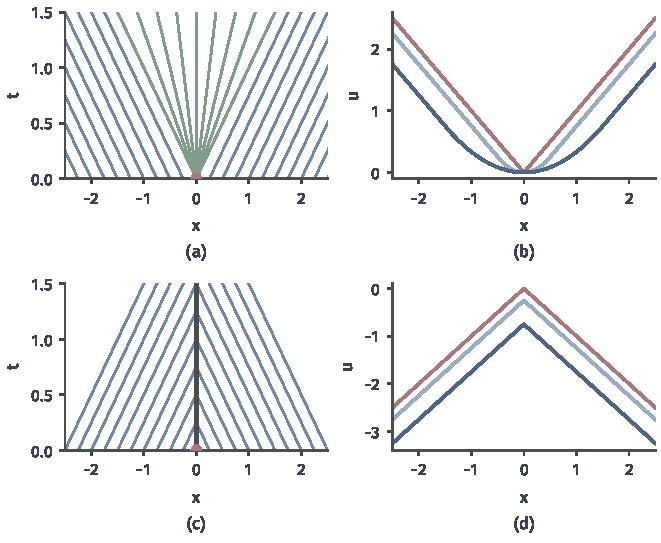
\includegraphics[width=112mm]{figures/06-differential-equations/02-partial-differential-equations/matplotlib/hj-fan-kink/figure.pdf}
  \caption{$H=p^2/2$下两种折角的演化。(a)、(b)$u_0=\lvert x\rvert$：折角处发出绿色扇形特征线填补空隙，解由式~\eqref{eq:hj-convex-kink}给出。(c)、(d)$u_0=-\lvert x\rvert$：蓝色特征线都汇入深灰的折角线，解由式~\eqref{eq:hj-concave-kink}给出。(b)、(d)中红线是初值，蓝色由浅到深是$t=0.5,1.5$。}
  \label{fig:hj-fan-kink}
\end{BookInlineFigure}

\paragraph{条件的作用}
凸性不能省略。公式只依赖$L=H^*$，而不同的$H$可能有相同的$L$。由Fenchel--Moreau定理，$L^*$是$H$的闭凸包，所以式~\eqref{eq:hj-hopf-lax}求解的其实是$H^{**}$对应的方程。若$H$不凸，$H^{**}\neq H$，公式给出的就不是原方程的解。

初值有界也用到了。对$u_0=-x^2/2$、$H=p^2/2$和$t>1$，公式中的目标函数
\[
  -\frac{y^2}{2}+\frac{(x-y)^2}{2t}
\]
的二次项系数是$\frac{1}{2t}-\frac12<0$，下确界是$-\infty$，公式失去意义。这和上一节经典解在$t=1$爆破是一致的。

\paragraph{到达时间：极限情形}
波前对应$H(\bm{p})=\lVert\bm{p}\rVert_2$，它是凸的，但只线性增长。此时共轭函数是单位球的指示函数：$\lVert\bm{q}\rVert_2\leq1$时$L(\bm{q})=0$，否则$L=+\infty$。把它代入式~\eqref{eq:hj-hopf-lax}，得到
\begin{equation}
  u(\bm{x},t)=\min_{\lVert\bm{y}-\bm{x}\rVert_2\leq t}u_0(\bm{y}).
  \label{eq:hj-erosion}
\end{equation}
定理~\ref{thm:hj-hopf-lax}不直接覆盖这种情形，但它的证明可以照搬：极小点在紧球上取得，半群性质只用到$L$的凸性，$\bm{q}_h$在单位球内，有界性不用再证，$H=L^*$仍然成立。所以式~\eqref{eq:hj-erosion}是有界Lipschitz初值下的黏性解。

这个公式说，$u$在$(\bm{x},t)$的值是初值在半径$t$的球内的最小值。取一个闭的源集$S$，$u_0=d(\cdot,S)$是到$S$的距离（要满足有界性，可以在远处截断，有限时间内的结果不受影响）。则
\[
  u(\bm{x},t)=\max\{d(\bm{x},S)-t,\ 0\},
\]
所以$\{u(\cdot,t)=0\}=\{d(\cdot,S)\leq t\}$恰好是时刻$t$已被扫过的区域，到达时间$T=d(\cdot,S)$从解中读出。

图~\ref{fig:hj-erosion}取一维的$S=\{-1.5,1\}$。相向的两列波前在$x=-0.25$、时刻$1.25$相遇，这正是图(b)的折角点。这与定理~\ref{thm:hj-distance}的结论一致，$T$就是到$S$的距离。

\begin{BookInlineFigure}
  \centering
  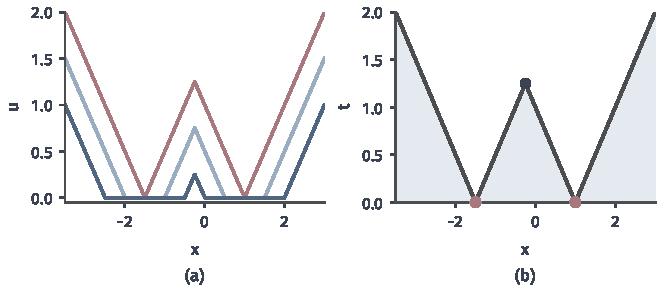
\includegraphics[width=112mm]{figures/06-differential-equations/02-partial-differential-equations/matplotlib/hj-erosion/figure.pdf}
  \caption{$H=\lvert p\rvert$的极限情形。(a)初值$u_0=d(x,S)$（红），$S=\{-1.5,1\}$，蓝色由浅到深是$t=0.5,1$的解，零值区域在扩大。(b)$(x,t)$平面，红点是源，深灰线是$T(x)=d(x,S)$，也就是四条波前的轨迹，浅蓝是波前尚未到达的区域$t<T(x)$，黑点$(-0.25,1.25)$是两列波前相遇的位置。}
  \label{fig:hj-erosion}
\end{BookInlineFigure}

Hopf--Lax公式的外形是在速度和代价之间做选择，让人想到控制问题。这一节只把它用作方程的表示公式：$L$由$H$算出来，极小化的作用是从特征线中选出黏性解。本章不需要问谁在做决策，也不需要讨论最优策略是否存在。

\section{消失黏性}
\label{sec:hj-vanishing}

第~\ref{chap:pde-problems}章已经见过，给程函方程加一个小扩散项，解的极限就是到边界的距离。这一节解释这个现象：在方程中加入$\varepsilon\Delta u$，光滑解在$\varepsilon\to0$时为什么收敛到黏性解，以及有限的$\varepsilon$下误差有多大。

考虑带小扩散的方程
\begin{equation}
  \partial_tu_\varepsilon+H(\nabla u_\varepsilon)=\varepsilon\Delta u_\varepsilon,\qquad u_\varepsilon(\cdot,0)=u_0,
  \label{eq:hj-viscous}
\end{equation}
其中$\varepsilon>0$。$\varepsilon$前面的符号与第~\ref{chap:diffusion-equations}章的热方程相同，时间向前是适定的。

\paragraph{一个可以精确求解的例子}
对$H=\lVert\bm{p}\rVert_2^2/2$，式~\eqref{eq:hj-viscous}可以化成线性的热方程。设$u_\varepsilon=-2\varepsilon\ln w$，$w>0$，这称为\term{Cole--Hopf变换}（Cole--Hopf transformation）。分别计算各项：
\[
  \partial_tu_\varepsilon=-2\varepsilon\frac{\partial_tw}{w},\qquad
  \frac12\lVert\nabla u_\varepsilon\rVert_2^2=2\varepsilon^2\frac{\lVert\nabla w\rVert_2^2}{w^2}.
\]
Laplace项为
\[
  \varepsilon\Delta u_\varepsilon=-2\varepsilon^2\frac{\Delta w}{w}+2\varepsilon^2\frac{\lVert\nabla w\rVert_2^2}{w^2}.
\]
代入式~\eqref{eq:hj-viscous}，含$\lVert\nabla w\rVert_2^2$的两项抵消，非线性消失了，剩下
\[
  \partial_tw=\varepsilon\Delta w.
\]

由第~\ref{chap:diffusion-equations}章的热核表示，$\partial_tw=\varepsilon\Delta w$在全空间的有界解是初值与Gauss核的卷积，初值取$w_0=\mathrm{e}^{-u_0/(2\varepsilon)}$。两个指数的自变量合并后，正好出现Hopf--Lax公式中的函数。记
\[
  F(\bm{y})=u_0(\bm{y})+\frac{\lVert\bm{x}-\bm{y}\rVert_2^2}{2t},
\]
则
\begin{equation}
  u_\varepsilon(\bm{x},t)=-2\varepsilon\ln\Bigl[(4\pi\varepsilon t)^{-d/2}\int_{\mathbb{R}^{d}}\mathrm{e}^{-F(\bm{y})/(2\varepsilon)}\,\mathrm{d}\bm{y}\Bigr].
  \label{eq:hj-cole-hopf}
\end{equation}

式~\eqref{eq:hj-cole-hopf}是一个“软极小”。图~\ref{fig:hj-cole-hopf-softmin}是$(x,t)=(0,\pi/2)$时的被积函数：$\varepsilon$变小时，权重集中到$F$的两个极小点附近，$-2\varepsilon\ln$把积分的值换算回$F$的尺度。

\begin{BookInlineFigure}
  \centering
  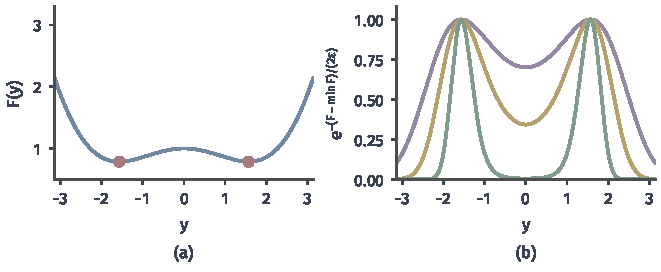
\includegraphics[width=112mm]{figures/06-differential-equations/02-partial-differential-equations/matplotlib/hj-cole-hopf-softmin/figure.pdf}
  \caption{Cole--Hopf公式中的权重，$u_0=\cos y$，$(x,t)=(0,\pi/2)$。(a)$F(y)$，红点是两个极小点。(b)归一化的被积函数，$\varepsilon=0.3$（紫）、$0.1$（黄）、$0.02$（绿）。$\varepsilon$变小时质量集中到极小点。}
  \label{fig:hj-cole-hopf-softmin}
\end{BookInlineFigure}

\begin{theorem}[Cole--Hopf解的极限]
\label{thm:hj-cole-hopf-limit}
设$u_0$有界且$R$-Lipschitz，$H=\lVert\bm{p}\rVert_2^2/2$，$u$是式~\eqref{eq:hj-hopf-lax}。对任意$0<t_1<t_2$，存在常数$C$，使对$t\in[t_1,t_2]$、$\bm{x}\in\mathbb{R}^{d}$和$0<\varepsilon\leq1/2$，
\begin{equation}
  \lvert u_\varepsilon(\bm{x},t)-u(\bm{x},t)\rvert\leq C\varepsilon\ln\frac{1}{\varepsilon}.
  \label{eq:hj-cole-hopf-limit}
\end{equation}
\end{theorem}

\begin{proof}
记$m=\min F=u(\bm{x},t)$，$M=\sup\lvert u_0\rvert$，$\bm{y}^*$为一个极小点。由$F(\bm{x})\leq M$，得$m\leq M$。

先估计积分的上界。由$u_0\geq-M$，得到
\[
  F(\bm{y})\geq-M+\frac{\lVert\bm{x}-\bm{y}\rVert_2^2}{2t}.
\]
取$\rho^2=8Mt$，当$\lVert\bm{x}-\bm{y}\rVert_2\geq\rho$时，
\[
  F(\bm{y})-m\geq\frac{\lVert\bm{x}-\bm{y}\rVert_2^2}{2t}-2M\geq\frac{\lVert\bm{x}-\bm{y}\rVert_2^2}{4t}.
\]
球内用$F\geq m$。合起来，记$\lvert B_\rho\rvert$为半径$\rho$的球的体积，得
\[
  \int\mathrm{e}^{-F/(2\varepsilon)}\,\mathrm{d}\bm{y}\leq\mathrm{e}^{-m/(2\varepsilon)}\bigl(\lvert B_\rho\rvert+(8\pi\varepsilon t)^{d/2}\bigr).
\]

再估计下界。由$\rho$的取法，极小点满足$\lVert\bm{x}-\bm{y}^*\rVert_2\leq\rho$。在$\bm{y}^*$的半径$\varepsilon$的球内，$F$是$\Lambda$-Lipschitz的，$\Lambda=R+(\rho+1)/t$，所以$F\leq m+\Lambda\varepsilon$，积分至少是
\[
  \mathrm{e}^{-m/(2\varepsilon)}\mathrm{e}^{-\Lambda/2}\lvert B_\varepsilon\rvert.
\]

把这两个界代入式~\eqref{eq:hj-cole-hopf}，$-2\varepsilon\ln$作用在$\mathrm{e}^{-m/(2\varepsilon)}$上得到$m$，其余因子是$\varepsilon$的幂次和$t\in[t_1,t_2]$上有界的常数，它们取对数再乘$2\varepsilon$后，不超过$C\varepsilon\ln(1/\varepsilon)$。
\end{proof}

所以在这个模型中，消失黏性的极限就是Hopf--Lax公式，也就是唯一的黏性解。

折角附近的结构也能精确算出。在$(0,\pi/2)$附近，$F$有两个极小点$\pm\pi/2$，$F''(\pm\pi/2)=2/\pi$，也就是$tF''=1$。把积分在两个极小点附近用Gauss积分近似，每个贡献$\sqrt{4\pi\varepsilon/F''}\,\mathrm{e}^{-\pi/(8\varepsilon)}$，于是
\begin{equation}
  u_\varepsilon(0,\pi/2)=\frac{\pi}{4}-2\varepsilon\ln2+O(\varepsilon^2).
  \label{eq:hj-kink-correction}
\end{equation}
其中$\ln2$来自“两个极小点”。表~\ref{tab:hj-kink-correction}用式~\eqref{eq:hj-cole-hopf}的数值积分核对，$\varepsilon$越小吻合得越好。

\begin{BookInlineTable}
  \centering
  \begin{tabular}{cccc}
    \toprule
    $\varepsilon$ & $0.2$ & $0.05$ & $0.01$\\
    \midrule
    $\pi/4-u_\varepsilon(0,\pi/2)$ & $0.2842$ & $0.0800$ & $0.0142$\\
    $2\varepsilon\ln2$ & $0.2773$ & $0.0693$ & $0.0139$\\
    \bottomrule
  \end{tabular}
  \caption{折角处的黏性修正，$u_0=\cos x$，$H=p^2/2$。}
  \label{tab:hj-kink-correction}
\end{BookInlineTable}

两条分支在$x=0$附近可以近似写成$\pi/4\pm x$，软极小给出
\[
  u_\varepsilon\approx\frac{\pi}{4}-2\varepsilon\ln\Bigl(2\cosh\frac{x}{2\varepsilon}\Bigr),\qquad
  \partial_xu_\varepsilon\approx-\tanh\frac{x}{2\varepsilon}.
\]
折角被抹成宽度约$\varepsilon$的过渡层，它的斜率恰好是第~\ref{chap:scalar-conservation-laws}章Burgers方程的黏性激波剖面。图~\ref{fig:hj-viscous-limit}显示这个过程。

\begin{BookInlineFigure}
  \centering
  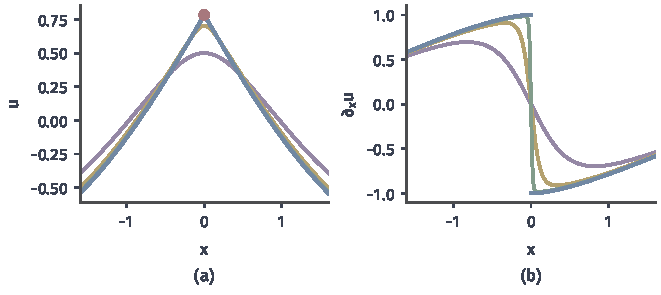
\includegraphics[width=112mm]{figures/06-differential-equations/02-partial-differential-equations/matplotlib/hj-viscous-limit/figure.pdf}
  \caption{消失黏性的极限，$u_0=\cos x$，$t=\pi/2$。(a)式~\eqref{eq:hj-cole-hopf}的$u_\varepsilon$，$\varepsilon=0.2$（紫）、$0.05$（黄）、$0.01$（绿），蓝线是Hopf--Lax解，红点是折角。(b)对应的斜率，$\varepsilon$变小时过渡层变窄，趋向蓝线在$x=0$的跳跃。}
  \label{fig:hj-viscous-limit}
\end{BookInlineFigure}

到达时间也有同样的线性化。令$T_\varepsilon=-\varepsilon\ln w$，代入带小扩散的方程
\[
  \lVert\nabla T_\varepsilon\rVert_2^2-\varepsilon\Delta T_\varepsilon=1,
\]
得到线性方程
\[
  \varepsilon^2\Delta w=w.
\]
第~\ref{chap:pde-problems}章的一维显式解就是$w=\cosh(x/\varepsilon)/\cosh(1/\varepsilon)$。

在平面上，点源的径向解是修正Bessel函数$K_0(r/\varepsilon)$，它满足$\varepsilon^2\Delta w=w$（$r>0$）。两个源的线性叠加给出
\[
  T_\varepsilon=-\varepsilon\ln\Bigl[K_0\bigl(\lVert\bm{x}-\bm{a}\rVert_2/\varepsilon\bigr)+K_0\bigl(\lVert\bm{x}-\bm{b}\rVert_2/\varepsilon\bigr)\Bigr].
\]
$K_0(z)$随$z$增大以$\mathrm{e}^{-z}$的速度衰减，所以$T_\varepsilon$是两个距离的软极小。图~\ref{fig:hj-soft-two-sources}显示，$\varepsilon$变小时，等值线向$T=\min\{T_1,T_2\}$靠拢，中垂线上的尖角由圆滑变尖锐。

\begin{BookInlineFigure}
  \centering
  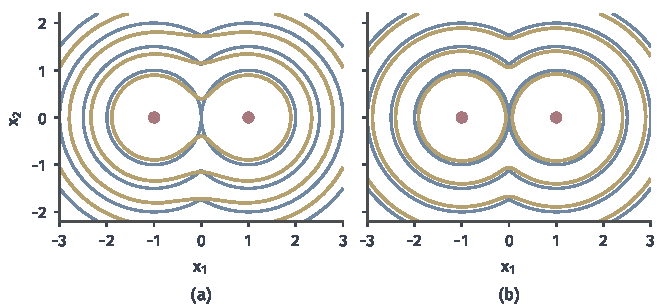
\includegraphics[width=112mm]{figures/06-differential-equations/02-partial-differential-equations/matplotlib/hj-soft-two-sources/figure.pdf}
  \caption{到达时间的软化，源为两个红点。蓝线是$T=\min\{T_1,T_2\}$的等值线$1,1.5,2,2.5$，黄线是$T_\varepsilon$的相同等值线。(a)$\varepsilon=0.3$。(b)$\varepsilon=0.08$。}
  \label{fig:hj-soft-two-sources}
\end{BookInlineFigure}

\paragraph{一般Hamilton量}
一般的$H$没有线性化，但结论不依赖显式解，其根据是黏性解在局部一致极限下稳定。

\begin{theorem}[黏性解的稳定性]
\label{thm:hj-stability-viscosity}
设$H$连续，$u_\varepsilon\in C^2$是式~\eqref{eq:hj-viscous}中方程的经典解，$\varepsilon\to0$时$u_\varepsilon\to u$在$\mathbb{R}^{d}\times(0,t_{\mathrm{f}})$上局部一致成立。则$u$是
\begin{equation}
  \partial_tu+H(\nabla u)=0
  \label{eq:hj-limit-equation}
\end{equation}
的黏性解。
\end{theorem}

\begin{proof}
只证次解，上解同理。设$\varphi\in C^1$，$u-\varphi$在$P$取局部极大。换成$\tilde\varphi=\varphi+\lVert\bm{z}-P\rVert_2^2$（$\bm{z}=(\bm{x},t)$），它在$P$的导数不变，且$u-\tilde\varphi$在$P$取严格局部极大。取以$P$为中心的闭球$B$，$B$在$t>0$内，使$P$是$u-\tilde\varphi$在$B$上唯一的最大点。

取光滑函数$\varphi^\eta$在$B$上连同一阶导数一致收敛到$\tilde\varphi$。固定$\eta$，$u_\varepsilon-\varphi^\eta$在$B$上的最大点记为$P_{\varepsilon}$。当它在$B$的内部时，一阶和二阶条件给出
\[
  \partial_t\varphi^\eta(P_\varepsilon)+H\bigl(\nabla\varphi^\eta(P_\varepsilon)\bigr)=\varepsilon\Delta u_\varepsilon(P_\varepsilon)\leq\varepsilon\Delta\varphi^\eta(P_\varepsilon).
\]

$\varphi^\eta$是固定的光滑函数，$\Delta\varphi^\eta$在$B$上有界。由一致收敛，$\varepsilon\to0$时$P_\varepsilon$的聚点是$u-\varphi^\eta$在$B$上的最大点；$\eta$充分小时这些点都靠近$P$，从而在$B$内部。令$\varepsilon\to0$，得到在某个最大点$P^\eta$处
\[
  \partial_t\varphi^\eta(P^\eta)+H\bigl(\nabla\varphi^\eta(P^\eta)\bigr)\leq0.
\]
再令$\eta\to0$，$P^\eta\to P$，$\varphi^\eta$的导数收敛到$\tilde\varphi$的导数，由$H$的连续性得到$\partial_t\varphi(P)+H(\nabla\varphi(P))\leq0$。
\end{proof}

证明只用到局部一致收敛，这就是黏性解在极限下稳定的原因。不需要梯度的强收敛，而对弱解来说，$H(\nabla u_\varepsilon)$的弱极限一般不是$H(\nabla u)$。

\begin{theorem}[消失黏性选择黏性解]
\label{thm:hj-vanishing-viscosity}
设$H$连续，$u_0$有界且$R$-Lipschitz。设对每个充分小的$\varepsilon$，式~\eqref{eq:hj-viscous}有$C^2$解$u_\varepsilon$，并且存在不依赖$\varepsilon$的常数$C$，使
\begin{equation}
  \lvert u_\varepsilon\rvert\leq C,\qquad\lVert\nabla u_\varepsilon\rVert_2\leq R,\qquad\lvert\partial_tu_\varepsilon\rvert\leq C.
  \label{eq:hj-uniform-estimates}
\end{equation}
则$\varepsilon\to0$时，$u_\varepsilon$局部一致收敛到初值问题唯一的有界、关于$\bm{x}$是$R$-Lipschitz的黏性解。
\end{theorem}

\begin{proof}
由式~\eqref{eq:hj-uniform-estimates}，$\{u_\varepsilon\}$一致有界且等度连续。由Arzel\`a--Ascoli定理，一致有界、等度连续的函数列在紧集上有一致收敛的子列。取任一收敛子列，极限$u$继承相同的界，由定理~\ref{thm:hj-stability-viscosity}是黏性解，$u(\cdot,0)=u_0$。

由定理~\ref{thm:hj-uniqueness}，这样的黏性解只有一个，所以所有收敛子列有相同的极限，整个族收敛。
\end{proof}

式~\eqref{eq:hj-uniform-estimates}是定理的条件，不是自动成立的。对光滑的$H(\bm{p})$，它们来自线性抛物方程的最大值原理：差商$u_\varepsilon(\bm{x}+\bm{h},t)-u_\varepsilon(\bm{x},t)$满足一个线性抛物方程，最大值在初始时刻取得，所以空间Lipschitz常数不增加，时间导数的界要求初值更光滑或先磨光初值。光滑解的存在性证明要用到抛物方程的正则性理论，篇幅较长，可查阅\scite{math-bardi1997hjb}。

所以$\varepsilon\Delta u$的作用和第~\ref{chap:scalar-conservation-laws}章在守恒律中的作用一样：它打破了对称，选择了一个解。$\varepsilon$的符号决定选哪个，这就是第~\ref{chap:pde-problems}章看到的符号问题。

\paragraph{有限黏性的误差}
$\varepsilon>0$时$u_\varepsilon$是光滑的，但它只是近似。一般的Lipschitz初值下，$\sup\lvert u_\varepsilon-u\rvert$的量级是$\sqrt{\varepsilon t}$，证明要用变量倍增并同时估计黏性项，篇幅较长，读者可查阅\scite{math-bardi1997hjb}。这个量级的含义是：在只有Lipschitz正则性时，误差随$\varepsilon$减小得比$\varepsilon$本身慢。在例~\ref{ex:hj-cos}中，由于解的结构特殊，$x=0$处的误差是$O(\varepsilon)$，见式~\eqref{eq:hj-kink-correction}和图~\ref{fig:hj-two-limits}(b)。

\paragraph{不要混淆两个极限}
实际计算时有两个参数：黏性$\varepsilon$和网格步长$h$。令$h\to0$只是更准确地解带$\varepsilon$的方程，令$\varepsilon\to0$才改变方程本身。

图~\ref{fig:hj-two-limits}(a)做了一个实验：固定$\varepsilon=0.1$，用周期网格上的中心差分和显式时间推进，时间步足够小，算到$t=\pi/2$。随着网格加密，到$u_\varepsilon$的误差按$h^2$下降，从$N=20$时的$0.056$降到$N=640$时的$6\times10^{-5}$。到$u$的误差却停在$0.159$附近，这是黏性解与带黏性方程的差，再细的网格也消除不了。

\begin{BookInlineFigure}
  \centering
  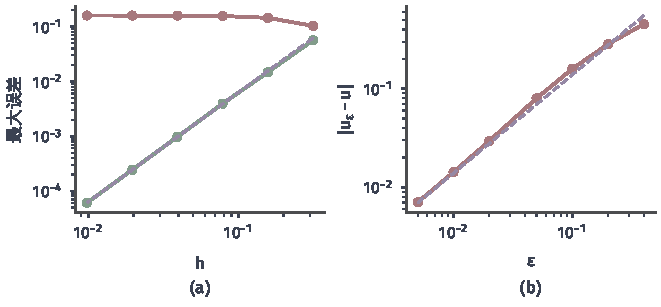
\includegraphics[width=112mm]{figures/06-differential-equations/02-partial-differential-equations/matplotlib/hj-two-limits/figure.pdf}
  \caption{两个极限的区分，$u_0=\cos x$，$t=\pi/2$。(a)固定$\varepsilon=0.1$，网格点数$N=20,\ldots,640$（$h=2\pi/N$），绿线是数值解到$u_\varepsilon$的最大误差，红线是到黏性解$u$的最大误差，紫色虚线是$h^2$的参考斜率。(b)式~\eqref{eq:hj-cole-hopf}在$x=0$处的误差随$\varepsilon$的变化，紫色虚线是$2\varepsilon\ln2$。}
  \label{fig:hj-two-limits}
\end{BookInlineFigure}

要逼近$u$本身，必须同时让$\varepsilon\to0$，并且让网格能够分辨宽度约$\varepsilon$的过渡层，或者在格式里内建适当的数值耗散。后一种做法把$\varepsilon$隐含在网格步长中，两个极限就合并了，这时收敛性需要专门的分析，不能从上面的实验推出。

\section{本章小结}
\label{sec:hj-summary}

本章围绕一个问题展开：当方程只限制局部的梯度时，场值由什么决定。到达时间给出了具体的图景，波前法向推进的速度决定$T$梯度的长度；令$u=T-t$，到达时间问题就进入时间依赖的方程，Hamilton量$H$说明斜率$\bm{p}$的地方高度下降多快。两类问题的数据不同，边值问题还要求数据相容。

光滑时，方程化为特征方程组。位置和斜率服从Hamilton方程，值靠一次积分带上，这样可以局部重建经典解。对波前而言，特征线就是射线，$u$沿线不变。

特征线会相交。一维中曲率按式~\eqref{eq:hj-riccati}发散，经典解在有限时刻结束，而斜率和场值依然有界。此后同一位置有多个候选，几乎处处满足方程的解不唯一，凹槽就是例子。

黏性解在接触点处提出不等式：从上方贴得到$\leq0$，从下方贴得到$\geq0$。它不做积分，也不移走导数，而且对方程的符号敏感。凹折角通过检验，凸折角不通过，这和“只有第一次到达才算数”是一致的。

比较原理把这些局部的不等式变成整体结论：次解和上解的次序从数据传到全部时刻，因此黏性解唯一，且对初值的依赖在上确界范数下不扩张。初值问题要有增长和连续性条件，边值问题要有$n>0$和相容的数据，两种情形的严格性来源不同，不能互相搬用。

存在性有两条途径。对凸且超线性增长的$H$，Hopf--Lax公式写出解，其极小点就是到达的特征线，取最小值就是选下包络，多个极小点的地方就是不可微点。消失黏性把解看成小扩散方程的极限，$H=\lVert\bm{p}\rVert_2^2/2$时Cole--Hopf变换让这件事可以精确计算；一般情形下依靠一致估计、局部一致收敛下的稳定性和比较原理。有限黏性下解仍有误差，加细网格也不能消除它。

表~\ref{tab:hj-summary}汇总各工具解决的问题和适用条件。

\begin{BookInlineTable}
  \centering
  \begin{tabular}{lll}
    \toprule
    工具 & 解决的问题 & 条件\\
    \midrule
    特征方程组 & 光滑范围内重建解 & $H$、$u_0$光滑，局部\\
    黏性解 & 不可微点上的选择 & 连续函数\\
    比较原理 & 唯一性与稳定性 & 增长、连续性、相容性\\
    Hopf--Lax公式 & 显式表示与存在性 & $H$凸且超线性\\
    消失黏性 & 光滑近似与解的选择 & 一致估计\\
    \bottomrule
  \end{tabular}
  \caption{本章各工具的作用。}
  \label{tab:hj-summary}
\end{BookInlineTable}

本章只做方程分析，所有结论都是有限时间内的。这里的$H$是给定的，Hopf--Lax公式中的极小化也只是解的表示。在决策问题中，Hamilton量由系统和代价确定，价值函数满足Hamilton--Jacobi--Bellman方程，需要进一步讨论价值函数与策略的验证，可参考\BookChapterRef{chap:continuous-time-optimal-control}{卷十第6章“连续时间最优控制”}。


\chapter{偏微分方程的数值求解}
\label{chap:pde-numerical-methods}

考虑区间上的边值问题：$-u''=\pi^2\sin(\pi x)$，$u(0)=0$，$u(1)=1$。它的解$u=\sin(\pi x)+x$可以直接写出，所以我们能核对任何近似。换成系数跳变的杆、形状不规则的板，或者会出现激波的车流，解就写不出来了。前面各章告诉我们解是否存在、属于什么空间、信息怎样传播，却没有告诉我们某一点的数值。

计算机只能保存有限个数，把一个场换成有限个数有不同的办法：记录格点上的值，记录一组基函数的系数，或者记录每个小单元里的平均量。这三种记录方式分别对应有限差分、Galerkin有限元和守恒有限体积方法，它们保留的是连续问题的三种不同结构：局部导数、弱形式和局部守恒。

得到一组数之后，真正难的问题才开始：这组数代表了什么？网格加密时它是否趋于原问题的解，趋于哪一个解？第~\ref{chap:scalar-conservation-laws}章已经看到，守恒律的弱解可以不唯一，一个看上去合理的格式完全可能收敛到错误的解。

本章先用上面的区间问题说明三类未知量和误差的三个来源，再依次讲三种方法，每种方法都结合能手算的小网格写出计算过程。随后讨论一致性、稳定性与收敛的关系，线性和非线性问题在这里要走不同的路。最后把空间、时间、积分和代数误差分开检验，并比较计算成本。

本章的结论都在有限时间区间上讨论，长时间行为不在这里考虑；除特别说明外，线性格式的结论针对规则网格。

\section{离散问题}
\label{sec:pdenum-discrete}

一个定义在区间上的函数有无穷多个值，怎样只用有限个数把它留下来？答案不止一种，不同的答案决定了后面的方程长什么样。全章的第一个例子是
\begin{equation}
 -u''=\pi^2\sin(\pi x)\quad\text{于}\ (0,1),\qquad u(0)=0,\quad u(1)=1,
 \label{eq:pdenum-model}
\end{equation}
它的解是
\begin{equation}
 u(x)=\sin(\pi x)+x .
 \label{eq:pdenum-model-exact}
\end{equation}

\paragraph{三类未知量}
把$[0,1]$等分成四段，步长$h=1/4$，节点$x_j=jh$。下面三种记录方式都只用几个数，含义却不同，图~\ref{fig:pdenum-three-unknowns}把它们画在同一个解上。

第一种记录节点上的值$U_j\approx u(x_j)$。这串数称为\term{网格函数}（grid function），它只在节点上有定义，节点之间是什么并不规定。有限差分方法的未知量就是它。

第二种记录一组基函数的系数$c_j$，把近似写成$u_h(x)=\sum_jc_j\varphi_j(x)$。$u_h$是定义在整个区间上的函数，可以求导、积分。若每个$\varphi_j$在节点$x_j$处为$1$、在其他节点处为$0$，系数恰好等于节点值，但它们的身份仍然是函数的坐标。有限元方法的未知量是它。

第三种把区间分成单元$C_j$，记录每个单元上的平均
\begin{equation}
 \bar{u}_j=\frac{1}{\lvert C_j\rvert}\int_{C_j}u\,\mathrm{d}x .
 \label{eq:pdenum-cell-average}
\end{equation}
它不是任何一点的值，而是这个单元里的总量除以长度。有限体积方法的未知量是它。

\begin{BookInlineFigure}
 \centering
 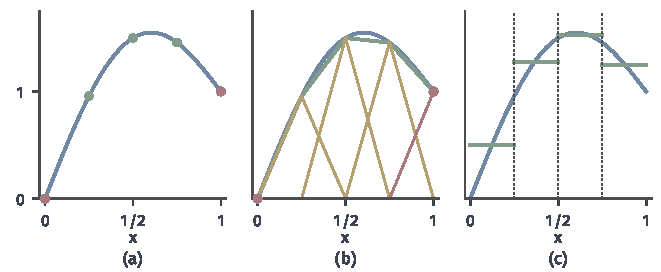
\includegraphics[width=112mm]{figures/06-differential-equations/02-partial-differential-equations/matplotlib/pdenum-three-unknowns/figure.pdf}
 \caption{同一个解$u=\sin(\pi x)+x$（蓝）的三种记录方式，$h=1/4$，红点是边值。(a)内部节点上的值（绿点）。(b)帽函数按节点值加权（黄线，右端红线是边界帽函数），其和是绿色折线。(c)四个单元上的平均（绿色水平线），虚线是单元界面。}
 \label{fig:pdenum-three-unknowns}
\end{BookInlineFigure}

把函数看成无限维向量，这三种做法都是在挑选有限个坐标：节点值是“按位置取样”，基函数系数是“在子空间里找坐标”，单元平均是“按小块累计”。类比到此为止，因为这三种坐标并不是同一个向量的不同分量，它们彼此之间相差一个与$h$有关的量。

例如在第一个单元$[0,1/4]$上，解的平均值由积分算出：
\[
 \bar{u}_1=4\int_0^{1/4}\bigl(\sin(\pi x)+x\bigr)\,\mathrm{d}x=\frac{4}{\pi}\Bigl(1-\frac{\sqrt2}{2}\Bigr)+\frac18\approx0.4979,
\]
而单元中点的值是$u(1/8)\approx0.5077$。比较数值解时必须说清比较的是哪一种量。

\paragraph{边界和初值怎样进入}
未知量选定后，还要说明已知数据放在哪里。Dirichlet边值是已知的节点值，它不再是未知量，而是把含它的项移到方程右端，右端因此带上边界数据。第~\ref{sec:pdenum-elliptic-fd}小节和第~\ref{sec:pdenum-weak-galerkin}小节会分别算出这一项。

Neumann条件和Robin条件规定的是边界通量。在弱形式和有限体积方法中，通量本来就在方程里出现，这些条件直接写进边界那一项；在差分格式中，则要用边界附近的差商或虚拟节点表达它们。

演化方程的初值$u_0$给出第一层数据，要按未知量的身份换算：差分取节点值，有限元取插值或投影，有限体积取单元平均。初值若不连续，这几种换算的差别并不小，后面的激波例子会用到单元平均。

\paragraph{三步离散，三份误差}
对演化方程，从$u$到屏幕上的数字要经过三步（图~\ref{fig:pdenum-error-pipeline}）。空间离散把场换成有限个未知量，得到第~\ref{chap:ode-numerical-methods}章讨论的常微分方程组；时间推进把它变成逐层的代数关系；每一层若含隐式方程，还要由有限精度的线性代数算出来。

\begin{BookInlineFigure}
 \centering
 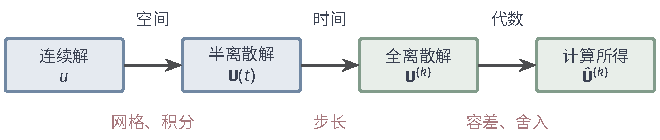
\includegraphics[width=112mm]{figures/06-differential-equations/02-partial-differential-equations/tikz/pdenum-error-pipeline/figure.pdf}
 \caption{从连续解到计算结果的三步。每个箭头引入一份误差，下方红字是控制它的主要因素。椭圆问题没有时间步，只有空间和代数两步。}
 \label{fig:pdenum-error-pipeline}
\end{BookInlineFigure}

记半离散解为$\bm{U}(t)$，全离散解为$\bm{U}^{(k)}$，实际算出的为$\widehat{\bm{U}}^{(k)}$，$\bm{R}_hu$表示把连续解按未知量的身份换算成离散向量。总误差分成三段：
\begin{equation}
 \begin{aligned}
 \bm{R}_hu(t_k)-\widehat{\bm{U}}^{(k)}
 &=\bigl(\bm{R}_hu(t_k)-\bm{U}(t_k)\bigr)\\
 &\quad+\bigl(\bm{U}(t_k)-\bm{U}^{(k)}\bigr)
 +\bigl(\bm{U}^{(k)}-\widehat{\bm{U}}^{(k)}\bigr).
 \end{aligned}
 \label{eq:pdenum-error-split}
\end{equation}

这样拆的好处是每一段可以单独控制，也可以单独检验。加密网格却不减小时间步，误差会停在时间误差的水平上；线性方程解得不够精确，误差会停在代数误差的水平上。第~\ref{sec:pdenum-error-cost}节会实际看到这两种停滞。

和常微分方程不同，这里步长变小时，向量$\bm{U}$的维数也在变。不同$h$对应的误差要能比较，范数必须随网格换算，比如$\lVert\bm{v}\rVert_{2,h}=(h\sum_jv_j^2)^{1/2}$相当于$L^2$范数，而$\lVert\bm{v}\rVert_\infty$相当于最大模。不带因子$h$的欧氏范数会随未知量增多而变大，不能用来比较。

\section{有限差分}
\label{sec:pdenum-finite-differences}

导数是极限，极限是算不完的，能算的是相邻几个值的差商。差商和导数差多少，由Taylor展开回答。

设$u$在$x$附近足够光滑。把$u(x\pm h)$在$x$处展开：
\[
 u(x\pm h)=u(x)\pm hu'(x)+\frac{h^2}{2}u''(x)\pm\frac{h^3}{6}u'''(x)+\frac{h^4}{24}u''''(\xi_\pm).
\]

只用一侧的值，得到前向差商和后向差商，它们与$u'(x)$相差$O(h)$。两式相减，偶次项消去，得到中心差商：
\begin{equation}
 \frac{u(x+h)-u(x-h)}{2h}=u'(x)+O(h^2).
 \label{eq:pdenum-central-first}
\end{equation}

两式相加，奇次项消去，得到二阶导数的三点公式：
\begin{equation}
 \delta_h^2u(x):=\frac{u(x-h)-2u(x)+u(x+h)}{h^2}=u''(x)+\frac{h^2}{12}u''''(\xi),
 \label{eq:pdenum-second-difference}
\end{equation}
其中$\xi\in(x-h,x+h)$，这里用到$u\in C^4$和介值定理，把两个余项合并成一个。

图~\ref{fig:pdenum-taylor-stencil}用$u=x^3$在$x=1$、$h=1/2$处比较三条割线。切线斜率是$3$，前向差商是$4.75$，后向差商是$1.75$，中心差商是$3.25$。两侧的偏差方向相反，取平均时一阶项抵消。

\begin{BookInlineFigure}
 \centering
 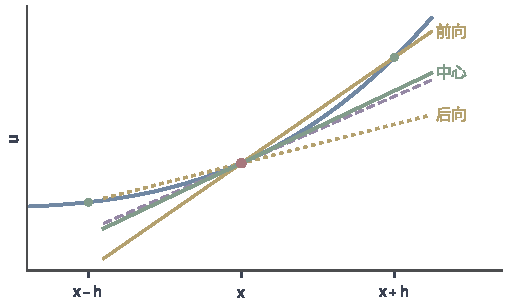
\includegraphics[width=86mm]{figures/06-differential-equations/02-partial-differential-equations/matplotlib/pdenum-taylor-stencil/figure.pdf}
 \caption{$u=x^3$（蓝）在红点$x=1$处的切线（紫色虚线）与三条差商割线，$h=1/2$。前向和后向差商（黄）分别偏大和偏小，中心差商（绿）的斜率$3.25$最接近切线的斜率$3$。}
 \label{fig:pdenum-taylor-stencil}
\end{BookInlineFigure}

余项里的$u''''$提醒我们：“二阶精度”不是公式本身的性质，而是公式加上解的光滑性的结论。解不够光滑时，式~\eqref{eq:pdenum-second-difference}的余项估计不成立，下面会看到实际阶数随之下降。

\subsection{椭圆方程的差分}
\label{sec:pdenum-elliptic-fd}

\paragraph{主要思想}
方程~\eqref{eq:pdenum-model}要求在每个内部节点$x_j$处成立，现在把它换成相邻三个节点值之间的关系。由式~\eqref{eq:pdenum-second-difference}，在$j=1,\ldots,n-1$上要求
\begin{equation}
 \frac{-U_{j-1}+2U_j-U_{j+1}}{h^2}=f(x_j),\qquad U_0=g_0,\quad U_n=g_1 .
 \label{eq:pdenum-three-point}
\end{equation}
这是$n-1$个未知量的线性方程组$\bm{A}_h\bm{U}=\bm{b}$。

边值出现在第一个和最后一个方程里。$j=1$的方程含已知的$U_0$，$j=n-1$的方程含已知的$U_n$，把它们移到右端，得到
\begin{equation}
 \bm{A}_h=\frac{1}{h^2}\begin{bmatrix}2&-1&&\\-1&2&\ddots&\\&\ddots&\ddots&-1\\&&-1&2\end{bmatrix},\qquad
 \bm{b}=\begin{bmatrix}f(x_1)+g_0/h^2\\f(x_2)\\\vdots\\f(x_{n-1})+g_1/h^2\end{bmatrix}.
 \label{eq:pdenum-fd-system}
\end{equation}

$\bm{A}_h$是三对角矩阵，按未知量的顺序消元时不产生新的非零元。一般的分解算法可参考\BookChapterRef{chap:direct-linear-solvers}{卷二第12章“线性方程的直接求解”}，这里只需要它的三对角形式。记对角元为$a_j$，上、下次对角元为$e_j$和$l_j$。消去第$j$行的下次对角元，逐行得到
\begin{equation}
 m_j=\frac{l_j}{d_{j-1}},\qquad d_j=a_j-m_je_{j-1},\qquad y_j=b_j-m_jy_{j-1}.
 \label{eq:pdenum-thomas-forward}
\end{equation}
消元后方程变成上双对角，再从最后一行往回代入：
\begin{equation}
 U_{n-1}=\frac{y_{n-1}}{d_{n-1}},\qquad U_j=\frac{y_j-e_jU_{j+1}}{d_j}.
 \label{eq:pdenum-thomas-back}
\end{equation}

\needspace{6\baselineskip}
\paragraph{变量}
\begin{itemize}
 \item $h=1/n$：步长；$x_j=jh$：节点，$j=0,\ldots,n$。
 \item $\bm{A}_h$：$(n-1)\times(n-1)$三对角矩阵，存为三个长度约$n$的数组。
 \item $\bm{b}\in\mathbb{R}^{n-1}$：节点上的右端，已含边值贡献。
 \item $d_j,y_j$：消元过程中的对角元和右端；$\bm{U}\in\mathbb{R}^{n-1}$：节点上的近似解。
\end{itemize}

\paragraph{初始化}
按式~\eqref{eq:pdenum-fd-system}填入$\bm{A}_h$与$\bm{b}$，并令$d_1=a_1$，$y_1=b_1$。

例中取$n=4$，$h=1/4$，$1/h^2=16$，$g_0=0$，$g_1=1$。节点上$f(x_j)=\pi^2\sin(\pi x_j)$，第三个方程的右端再加上$g_1/h^2=16$，于是
\[
 \bm{A}_h=16\begin{bmatrix}2&-1&0\\-1&2&-1\\0&-1&2\end{bmatrix},\qquad
 \bm{b}=\begin{bmatrix}6.9789\\9.8696\\22.9789\end{bmatrix}.
\]
初值是$d_1=32$，$y_1=6.9789$。

\needspace{6\baselineskip}
\paragraph{每轮更新}
对$j=2,\ldots,n-1$依次执行下面两步，第$n-1$行处理完后结束消元。
\begin{enumerate}
 \item 由式~\eqref{eq:pdenum-thomas-forward}算出$m_j,d_j$。例中第一轮$j=2$，第二轮$j=3$：
 \[
  \begin{aligned}
  m_2&=\frac{-16}{32}=-0.5, & d_2&=32-(-0.5)(-16)=24,\\
  m_3&=\frac{-16}{24}=-0.6667, & d_3&=32-(-0.6667)(-16)=21.3333.
  \end{aligned}
 \]
 \item 由同一式更新右端。例中两轮分别是
 \[
  \begin{aligned}
  y_2&=9.8696+0.5\times6.9789=13.3590,\\
  y_3&=22.9789+0.6667\times13.3590=31.8849.
  \end{aligned}
 \]
\end{enumerate}

消元结束后按式~\eqref{eq:pdenum-thomas-back}从下往上回代。例中依次得到
\[
 U_3=\frac{31.8849}{21.3333}=1.4946,\qquad
 U_2=\frac{13.3590+16\times1.4946}{24}=1.5530,
\]
\[
 U_1=\frac{6.9789+16\times1.5530}{32}=0.9946.
\]

最终得到节点上的近似解$(0.9946,\,1.5530,\,1.4946)$。式~\eqref{eq:pdenum-model-exact}给出的真值是$(0.9571,\,1.5000,\,1.4571)$，三个误差依次为$0.0375$、$0.0530$、$0.0375$。

\begin{BookInlineFigure}
 \centering
 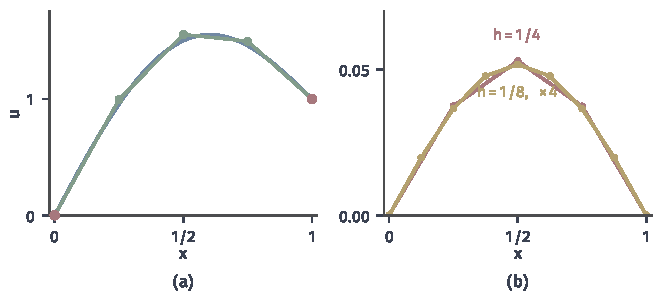
\includegraphics[width=112mm]{figures/06-differential-equations/02-partial-differential-equations/matplotlib/pdenum-fd-solution/figure.pdf}
 \caption{三点格式解问题~\eqref{eq:pdenum-model}。(a)$h=1/4$的数值解（绿）与真解（蓝），红点是边值。(b)节点误差，红线为$h=1/4$，黄线为$h=1/8$的误差乘以$4$：两条折线几乎重合，说明误差按$h^2$减小。}
 \label{fig:pdenum-fd-solution}
\end{BookInlineFigure}

图~\ref{fig:pdenum-fd-solution}(b)显示步长减半时误差约变为四分之一。这件事为什么成立？每个方程的残差很小，并不直接说明解的误差很小，下面要把两者联系起来。

\paragraph{从残差到误差}
把真解的节点值$\bm{R}_hu$代入离散方程，方程不再精确成立，差值就是\term{截断误差}（truncation error）：
\begin{equation}
 \bm{\tau}_h=\bm{A}_h\bm{R}_hu-\bm{b}.
 \label{eq:pdenum-truncation}
\end{equation}
由式~\eqref{eq:pdenum-second-difference}，$u\in C^4[0,1]$时它的每个分量满足$\lvert\tau_j\rvert\leq h^2M_4/12$，其中$M_4=\max\lvert u''''\rvert$。

离散解的误差$\bm{e}=\bm{R}_hu-\bm{U}$满足$\bm{A}_h\bm{e}=\bm{\tau}_h$，所以$\bm{e}=\bm{A}_h^{-1}\bm{\tau}_h$。问题归结为$\bm{A}_h^{-1}$的大小，而且这个大小不能随$h$变小而变大。这里要注意，$\bm{A}_h$的元素是$h^{-2}$量级，直接看它的元素说明不了逆的大小。

连续问题中，最大值原理控制了$-u''=f$的解（第~\ref{chap:elliptic-equations}章）。离散问题有完全平行的结论，证明也更短，因为“最大值点”只需在有限个数里找。

\begin{theorem}[离散最大值原理]
 \label{thm:pdenum-discrete-maximum}
 设网格函数$v_0,\ldots,v_n$在每个内部节点满足
 \begin{equation}
  \frac{-v_{j-1}+2v_j-v_{j+1}}{h^2}\leq0,\qquad j=1,\ldots,n-1,
  \label{eq:pdenum-discrete-subharmonic}
 \end{equation}
 则$\max_jv_j=\max(v_0,v_n)$。
\end{theorem}

\begin{proof}
 设最大值$M$在某个内部节点$j$取到。条件~\eqref{eq:pdenum-discrete-subharmonic}可以写成
 \[
  v_j\leq\frac{v_{j-1}+v_{j+1}}{2}.
 \]
 两个邻点都不超过$M$，而它们的平均不小于$v_j=M$，所以两个邻点都等于$M$。

 对邻点重复这个论证，最大值一路传到端点，于是$v_0=M$（也有$v_n=M$）。若最大值不在内部取到，它已经在端点上。
\end{proof}

这个定理的直观内容与热的抹平一致：每一点都不高于两邻点的平均，就不可能自己鼓起一个包。用它可以估计逆矩阵，诀窍是找一个差分算子作用后恰好等于$1$的函数。

\begin{theorem}[三点格式的误差界]
 \label{thm:pdenum-fd-error}
 对任意$\bm{\tau}\in\mathbb{R}^{n-1}$，$\bm{A}_h\bm{e}=\bm{\tau}$的解满足
 \begin{equation}
  \lVert\bm{e}\rVert_\infty\leq\frac18\lVert\bm{\tau}\rVert_\infty .
  \label{eq:pdenum-inverse-bound}
 \end{equation}
 若问题的解$u\in C^4[0,1]$，则
 \begin{equation}
  \max_j\lvert u(x_j)-U_j\rvert\leq\frac{h^2}{96}\max_{[0,1]}\lvert u''''\rvert .
  \label{eq:pdenum-fd-error}
 \end{equation}
\end{theorem}

\begin{proof}
 取$w(x)=x(1-x)/2$。它是二次函数，式~\eqref{eq:pdenum-second-difference}的余项为零，所以$-\delta_h^2w=-w''=1$，即$w$的节点值满足$\bm{A}_hw=\bm{1}$。

 令$v_j=e_j-\lVert\bm{\tau}\rVert_\infty w(x_j)$，并约定$e_0=e_n=0$。则$v_0=v_n=0$，且在内部节点上
 \[
  \frac{-v_{j-1}+2v_j-v_{j+1}}{h^2}=\tau_j-\lVert\bm{\tau}\rVert_\infty\leq0 .
 \]

 由定理~\ref{thm:pdenum-discrete-maximum}，$v_j\leq0$，即$e_j\leq\lVert\bm{\tau}\rVert_\infty w(x_j)$。对$-\bm{e}$作同样的论证，得到
 \[
  \lvert e_j\rvert\leq\lVert\bm{\tau}\rVert_\infty w(x_j) .
 \]

 $w$的最大值是$w(1/2)=1/8$，式~\eqref{eq:pdenum-inverse-bound}成立。把$\lVert\bm{\tau}_h\rVert_\infty\leq h^2M_4/12$代入，得到式~\eqref{eq:pdenum-fd-error}。
\end{proof}

证明的结构是后面反复出现的模式：一致性给出小的残差，稳定性（这里是$\lVert\bm{A}_h^{-1}\rVert_\infty\leq1/8$，常数与$h$无关）把残差转成解的误差。

例中$u''''=\pi^4\sin(\pi x)$，$M_4=\pi^4$，表~\ref{tab:pdenum-fd-refine}比较实际误差与上界。

\begin{BookInlineTable}
 \centering
 \caption{三点格式解问题~\eqref{eq:pdenum-model}的最大模误差和式~\eqref{eq:pdenum-fd-error}的上界。}
 \label{tab:pdenum-fd-refine}
 \begin{tabular}{cccc}
  \toprule
  $n$ & 实际误差 & 上界 & 相邻误差之比\\
  \midrule
  $4$ & $5.303\times10^{-2}$ & $6.342\times10^{-2}$ & --\\
  $8$ & $1.295\times10^{-2}$ & $1.585\times10^{-2}$ & $4.09$\\
  $16$ & $3.219\times10^{-3}$ & $3.964\times10^{-3}$ & $4.02$\\
  $32$ & $8.036\times10^{-4}$ & $9.909\times10^{-4}$ & $4.01$\\
  \bottomrule
 \end{tabular}
\end{BookInlineTable}

\paragraph{光滑性不够时}
误差界要求$u\in C^4$。换一个解$u=x^{3/2}-x$，它满足$u(0)=u(1)=0$，源项$f=-\tfrac34x^{-1/2}$在内部节点上有定义，但$u''$在$x=0$处无界，定理的条件不满足。

\begin{BookInlineFigure}
 \centering
 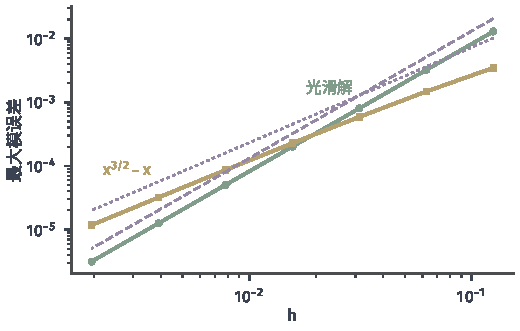
\includegraphics[width=88mm]{figures/06-differential-equations/02-partial-differential-equations/matplotlib/pdenum-fd-rates/figure.pdf}
 \caption{三点格式的网格加密，$n$从$8$到$512$，绿线是光滑解$\sin(\pi x)+x$，黄线是$x^{3/2}-x$。紫色虚线是斜率$2$，紫色点线是斜率$3/2$的参考线。公式没有改变，实际的收敛阶却取决于解的光滑性。}
 \label{fig:pdenum-fd-rates}
\end{BookInlineFigure}

图~\ref{fig:pdenum-fd-rates}是实际结果。光滑解每次加密的观测阶稳定在$2.00$附近。$x^{3/2}-x$的观测阶依次为$1.23$、$1.33$、$1.37$、$1.40$、$1.43$、$1.44$，逐渐向$3/2$靠近。这就是不能只凭公式形式判断精度的原因。

\paragraph{规则网格上的Poisson格式}
到两个空间维，在单位正方形上取步长$h$的规则网格。把$x_1$方向和$x_2$方向的三点公式相加，得到五点公式：
\begin{equation}
 \frac{4U_{i,j}-U_{i-1,j}-U_{i+1,j}-U_{i,j-1}-U_{i,j+1}}{h^2}=f(\bm{x}_{i,j}) .
 \label{eq:pdenum-five-point}
\end{equation}

边界上的节点值已知，出现时同样移到右端。图~\ref{fig:pdenum-five-point}(a)是模板的系数，(b)是$h=1/3$的网格，只有绿色的四个节点是未知量。

\begin{BookInlineFigure}
 \centering
 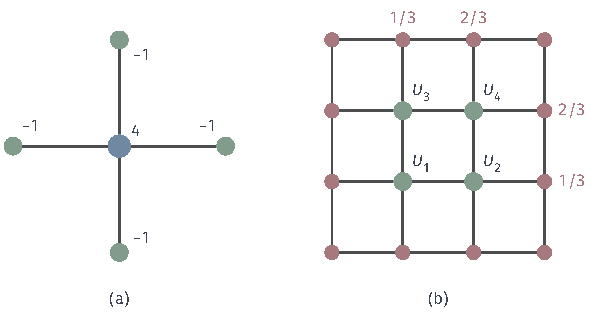
\includegraphics[width=101mm]{figures/06-differential-equations/02-partial-differential-equations/tikz/pdenum-five-point/figure.pdf}
 \caption{(a)五点模板，中心系数$4$，四个邻点系数$-1$，整体除以$h^2$。(b)$h=1/3$的网格，绿点是未知量，红点是已知的边值。边界标注是例子中边值$g=x_1x_2$在右边和上边的取值，左边和下边$g=0$。}
 \label{fig:pdenum-five-point}
\end{BookInlineFigure}

取$-\Delta u=0$，边值$g=x_1x_2$，真解就是$u=x_1x_2$。按图中编号，例如$U_2$的方程含右邻的边值$g(1,1/3)=1/3$，$U_4$的方程含右邻$g(1,2/3)$和上邻$g(2/3,1)$。乘以$h^2$并把边值移到右端，方程组是
\begin{equation}
 \begin{bmatrix}4&-1&-1&0\\-1&4&0&-1\\-1&0&4&-1\\0&-1&-1&4\end{bmatrix}
 \begin{bmatrix}U_1\\U_2\\U_3\\U_4\end{bmatrix}
 =\begin{bmatrix}0\\1/3\\1/3\\4/3\end{bmatrix}.
 \label{eq:pdenum-five-point-example}
\end{equation}

利用对称性$U_2=U_3$。第一个方程给出
\[
 U_2=2U_1 .
\]
代入第二个方程，得到
\[
 U_4=7U_1-\frac13 .
\]
最后一个方程成为$4U_4-2U_2=4/3$，代入上面两式，
\[
 24U_1=\frac83,\qquad U_1=\frac19,\quad U_2=U_3=\frac29,\quad U_4=\frac49 .
\]
这正是$x_1x_2$在四个节点上的值。原因是$x_1x_2$的四阶导数全为零，截断误差为零。

一般情形的误差估计与一维相同。设$u\in C^4(\overline{\Omega})$，比较函数仍取$w=x_1(1-x_1)/2$，它在五点算子下也给出$1$，所以$\lVert\bm{A}_h^{-1}\rVert_\infty\leq1/8$，最大模误差不超过$(h^2/96)(\max\lvert\partial_1^4u\rvert+\max\lvert\partial_2^4u\rvert)$。

矩阵的结构发生了变化。图~\ref{fig:pdenum-matrix-pattern}中，一维矩阵的非零元贴着对角线，二维矩阵除三条对角线外，还有两条离对角线一整行网格之远的带。按行消元时，带内的零元会被填满，所以二维问题的直接分解远比一维昂贵，第~\ref{sec:pdenum-error-cost}节再讨论这个代价。

\begin{BookInlineFigure}
 \centering
 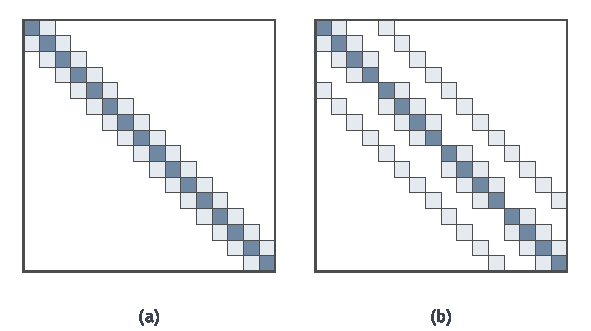
\includegraphics[width=100mm]{figures/06-differential-equations/02-partial-differential-equations/matplotlib/pdenum-matrix-pattern/figure.pdf}
 \caption{差分矩阵的非零元位置，深色是对角元。(a)一维三点格式，$16$个未知量。(b)二维五点格式，$4\times4$个内部节点，共$16$个未知量，按行编号。这里的方格本身是矩阵元素。}
 \label{fig:pdenum-matrix-pattern}
\end{BookInlineFigure}

规则网格的方便之处也是限制。边界不沿网格线时，靠近边界的节点需要专门的不等距模板，矩阵的对称性和最大值性质都要重新检查。下一节的有限元方法从弱形式出发，处理一般区域要自然得多。

\subsection{扩散方程的差分}
\label{sec:pdenum-heat-fd}

现在让温度随时间变化。考虑
\begin{equation}
 \partial_tu=\partial_x^2u\quad\text{于}\ (0,1)\times(0,T],\qquad u(0,t)=u(1,t)=0,\quad u(x,0)=u_0(x).
 \label{eq:pdenum-heat}
\end{equation}
这里只对空间做上一小节的离散，把时间留到下一步，这种做法称为\term{半离散}（semi-discretization）。

\paragraph{主要思想}
在内部节点上用三点公式代替$\partial_x^2u$，时间仍然连续，就得到常微分方程组
\begin{equation}
 \dot{\bm{U}}(t)=-\bm{A}_h\bm{U}(t),\qquad \bm{U}(0)=\bm{R}_hu_0 .
 \label{eq:pdenum-semidiscrete}
\end{equation}
偏微分方程变成了第~\ref{chap:ode-numerical-methods}章的线性系统，这正是把函数看成无限维向量所期待的对应：算子$\partial_x^2$对应矩阵$-\bm{A}_h$，它的特征模式对应矩阵的特征向量。

矩阵的特征向量恰好是正弦函数在节点上的取样。用三角恒等式
\[
 \sin(m\pi(j-1)h)+\sin(m\pi(j+1)h)=2\cos(m\pi h)\sin(m\pi jh)
\]
代入，得到$\bm{A}_h$的特征值
\begin{equation}
 \lambda_m=\frac{4}{h^2}\sin^2\frac{m\pi h}{2},\qquad m=1,\ldots,n-1 .
 \label{eq:pdenum-discrete-eigenvalues}
\end{equation}

$h\to0$时对固定的$m$有$\lambda_m\to m^2\pi^2$，这是连续算子的特征值。但$m$接近$n$时情形完全不同：最大特征值$\lambda_{n-1}=(4/h^2)\cos^2(\pi h/2)$接近$4/h^2$。

\begin{BookInlineFigure}
 \centering
 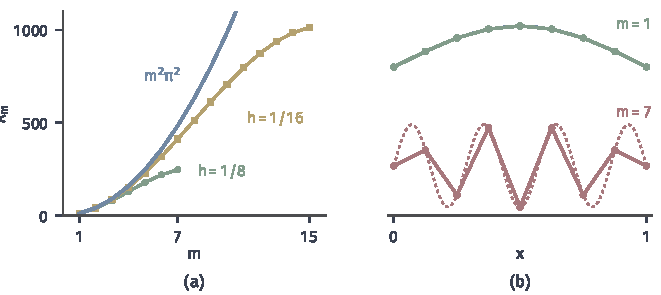
\includegraphics[width=112mm]{figures/06-differential-equations/02-partial-differential-equations/matplotlib/pdenum-heat-modes/figure.pdf}
 \caption{(a)连续特征值$m^2\pi^2$（蓝）与差分矩阵的特征值（绿$h=1/8$，黄$h=1/16$）。低模式贴近蓝线，高模式明显偏低，而网格越细，最大特征值越大。(b)$h=1/8$上的两个模式，绿线$m=1$，红线$m=7$；虚线是对应的连续正弦。}
 \label{fig:pdenum-heat-modes}
\end{BookInlineFigure}

图~\ref{fig:pdenum-heat-modes}说明了网格变细时发生的事。网格加密引入了越来越快的衰减模式，这些锯齿模式在真解中早已消失，也不是我们想算的东西，却决定了显式方法的步长上限。这与第~\ref{chap:ode-numerical-methods}章的刚性问题是同一件事。

在时间方向上，用步长$\tau$对式~\eqref{eq:pdenum-semidiscrete}作三种推进。三者的迭代公式为
\begin{align}
 \bm{U}^{(k+1)}&=(\bm{I}-\tau\bm{A}_h)\bm{U}^{(k)},
 \label{eq:pdenum-ftcs}\\
 \bm{U}^{(k+1)}&=(\bm{I}+\tau\bm{A}_h)^{-1}\bm{U}^{(k)},
 \label{eq:pdenum-btcs}\\
 \bm{U}^{(k+1)}&=\Bigl(\bm{I}+\frac{\tau}{2}\bm{A}_h\Bigr)^{-1}\Bigl(\bm{I}-\frac{\tau}{2}\bm{A}_h\Bigr)\bm{U}^{(k)}.
 \label{eq:pdenum-cn}
\end{align}
它们依次是显式Euler方法、后向Euler方法和\term{Crank--Nicolson方法}（Crank--Nicolson method）。第三种是梯形方法用在式~\eqref{eq:pdenum-semidiscrete}上的结果。

记$r=\tau/h^2$，式~\eqref{eq:pdenum-ftcs}的分量形式是
\begin{equation}
 U_j^{(k+1)}=U_j^{(k)}+r\bigl(U_{j-1}^{(k)}-2U_j^{(k)}+U_{j+1}^{(k)}\bigr).
 \label{eq:pdenum-ftcs-component}
\end{equation}

\needspace{6\baselineskip}
\paragraph{变量}
\begin{itemize}
 \item $\bm{U}^{(k)}\in\mathbb{R}^{n-1}$：第$k$层内部节点上的近似值。
 \item $h,\tau,r=\tau/h^2$：空间步、时间步及它们的比值。
 \item 后向Euler方法和Crank--Nicolson方法还要保存三对角矩阵及其消元结果$d_j$。
\end{itemize}

\paragraph{初始化}
令$U_j^{(0)}=u_0(x_j)$。例中取$h=1/4$，$u_0=\sin(\pi x)+0.1\sin(3\pi x)$，由它的两个模式可以写出真解：
\begin{equation}
 u(x,t)=\mathrm{e}^{-\pi^2t}\sin(\pi x)+0.1\,\mathrm{e}^{-9\pi^2t}\sin(3\pi x).
 \label{eq:pdenum-heat-exact}
\end{equation}
三个节点上的初值是
\[
 \bm{U}^{(0)}=(0.7778,\,0.9000,\,0.7778)^\top .
\]

\needspace{6\baselineskip}
\paragraph{每轮更新}
显式格式每轮按式~\eqref{eq:pdenum-ftcs-component}对$j=1,\ldots,n-1$算一遍，边界值$U_0=U_n=0$不更新，到$k\tau=T$结束。

例中先取$\tau=0.03$，$r=0.48$。第一轮中间节点的值是
\[
 U_2^{(1)}=0.9+0.48(0.7778-1.8+0.7778)=0.7827,
\]
左节点的值是
\[
 U_1^{(1)}=0.7778+0.48(0-1.5556+0.9)=0.4631 .
\]
此后各轮的结果为
\[
 \begin{aligned}
 \bm{U}^{(1)}&=(0.4631,\,0.7827,\,0.4631)^\top,\\
 \bm{U}^{(2)}&=(0.3942,\,0.4759,\,0.3942)^\top,\\
 \bm{U}^{(3)}&=(0.2442,\,0.3975,\,0.2442)^\top.
 \end{aligned}
\]
数值解有些摆动，但在衰减。把时间步改成$\tau=0.05$，$r=0.8$，前四轮是
\[
 \begin{aligned}
 \bm{U}^{(1)}&=(0.2533,\,0.7045,\,0.2533)^\top,\\
 \bm{U}^{(2)}&=(0.4116,\,-0.0174,\,0.4116)^\top,\\
 \bm{U}^{(3)}&=(-0.2609,\,0.6690,\,-0.2609)^\top,\\
 \bm{U}^{(4)}&=(0.6918,\,-0.8189,\,0.6918)^\top.
 \end{aligned}
\]
真解在$t=0.2$时中点的值是$0.1389$，而数值解已经变号并开始放大。

后向Euler方法每轮解一个三对角方程，用式~\eqref{eq:pdenum-thomas-forward}和式~\eqref{eq:pdenum-thomas-back}，矩阵的对角元是$1+2r$，次对角元是$-r$。例中$\tau=0.05$，$r=0.8$，第一轮的消元过程是
\[
 \begin{aligned}
 m_2&=-0.3077, & d_2&=2.3538, & y_2&=1.1393,\\
 m_3&=-0.3399, & d_3&=2.3281, & y_3&=1.1650,
 \end{aligned}
\]
从$d_1=2.6$和$y_1=0.7778$出发。回代给出
\[
 \bm{U}^{(1)}=(0.5004,\,0.6541,\,0.5004)^\top .
\]
第二、第三轮分别得到中点值$0.4565$和$0.3138$。同一个$\tau$下，Crank--Nicolson方法前三轮的中点值是$0.6358$、$0.3824$、$0.2391$，而真解是$0.6093$、$0.3727$、$0.2275$。它们都不放大。最终得到的是一列随时间衰减的向量，比较结果见下面对放大因子的分析。

\paragraph{放大因子解释一切}
对每个模式，$-\tau\lambda_m=z$，三种格式分别把这个模式乘上
\begin{equation}
 R_{\mathrm{E}}(z)=1+z,\qquad R_{\mathrm{B}}(z)=\frac{1}{1-z},\qquad R_{\mathrm{CN}}(z)=\frac{1+z/2}{1-z/2}.
 \label{eq:pdenum-heat-factors}
\end{equation}

例中$\lambda_1,\lambda_2,\lambda_3$分别约为$9.37$、$32$、$54.63$。$\tau=0.05$时，$R_{\mathrm{E}}$在三个模式上取$0.531$、$-0.6$、$-1.731$，第三个模式的绝对值大于$1$，放大的正是这个模式；$\tau=0.03$时，三个值是$0.719$、$0.04$、$-0.639$。图~\ref{fig:pdenum-amplification}把三条放大因子曲线和例中的点画在一起。

\begin{BookInlineFigure}
 \centering
 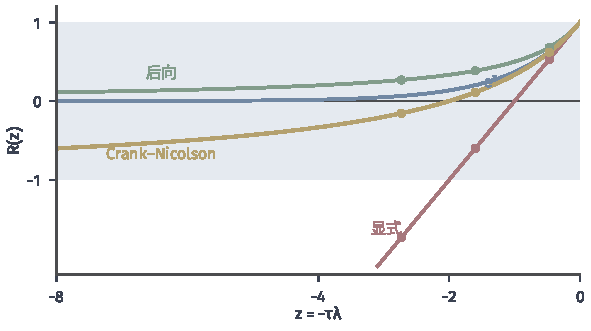
\includegraphics[width=100mm]{figures/06-differential-equations/02-partial-differential-equations/matplotlib/pdenum-amplification/figure.pdf}
 \caption{负实轴上的放大因子：蓝线是真解的$\mathrm{e}^{z}$，红线是显式Euler方法，绿线是后向Euler方法，黄线是Crank--Nicolson方法。浅蓝带表示$\lvert R\rvert\leq1$。圆点是$h=1/4$，$\tau=0.05$时三个模式的$z$值，显式Euler方法最左边的红点已在带外。}
 \label{fig:pdenum-amplification}
\end{BookInlineFigure}

显式格式要求所有模式都有$\lvert1+z\rvert\leq1$，即
\begin{equation}
 \tau\lambda_{\max}\leq2 .
 \label{eq:pdenum-ftcs-stability}
\end{equation}
由于$\lambda_{\max}<4/h^2$，$r=\tau/h^2\leq1/2$对任何网格都足够。例中$2/\lambda_{\max}=0.0366$，所以$\tau=0.03$稳定，$\tau=0.05$不稳定。

图~\ref{fig:pdenum-heat-stability}在$h=1/20$上比较阈值两侧。初值加了一个$2\times10^{-5}$大小的锯齿模式，它代表实际计算中总会出现的微小扰动。$r=0.55$时，这个几乎看不见的模式每步放大约$1.19$倍，到$t=0.08$时已经把解淹没。

\begin{BookInlineFigure}
 \centering
 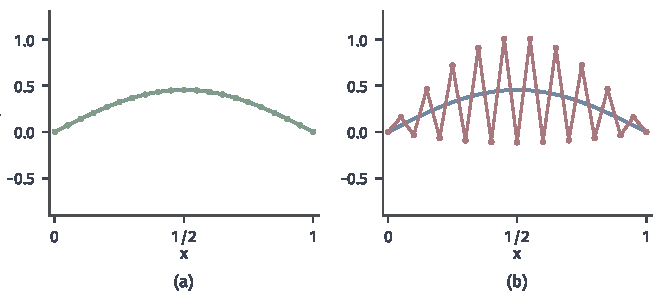
\includegraphics[width=112mm]{figures/06-differential-equations/02-partial-differential-equations/matplotlib/pdenum-heat-stability/figure.pdf}
 \caption{显式Euler方法在$h=1/20$上解式~\eqref{eq:pdenum-heat}到$t=0.08$，蓝线是真解。初值$\sin(\pi x)+0.1\sin(3\pi x)$叠加了幅度$2\times10^{-5}$的$\sin(19\pi x)$。(a)$r=0.4$，绿线贴合真解。(b)$r=0.55$，红线成为节点间振荡的锯齿。}
 \label{fig:pdenum-heat-stability}
\end{BookInlineFigure}

后向Euler方法对任何$z<0$都有$0<R_{\mathrm{B}}<1$，Crank--Nicolson方法也有$\lvert R_{\mathrm{CN}}\rvert<1$，它们都是无条件稳定的。但两者并不等价。$z\to-\infty$时，$R_{\mathrm{B}}\to0$，$R_{\mathrm{CN}}\to-1$，也就是说Crank--Nicolson方法几乎不衰减高模式，只是让它们每步变号。

\begin{BookInlineFigure}
 \centering
 \includegraphics[width=112mm]{figures/06-differential-equations/02-partial-differential-equations/matplotlib/pdenum-cn-oscillation/figure.pdf}
 \caption{方波初值、$h=1/40$、$\tau=0.02$（$r=32$）走三步。蓝线是半离散系统的精确解。(a)后向Euler方法（绿）光滑，略有偏差。(b)Crank--Nicolson方法（黄）在间断附近保留了振荡，此时最高模式的放大因子约为$-0.97$。}
 \label{fig:pdenum-cn-oscillation}
\end{BookInlineFigure}

图~\ref{fig:pdenum-cn-oscillation}是这个差别的后果。初值的跳跃含有大量高模式，$r$很大时，Crank--Nicolson方法在跳跃处留下不衰减的尖峰，而真解在第一瞬间就把它们抹平了。“无条件稳定”只是说不放大，并不保证解的外观正确。

\paragraph{精度和稳定对步长的不同要求}
稳定性问的是误差会不会放大，精度问的是每步新引入多少误差。Taylor展开给出三种格式的截断误差：两种Euler方法是$O(\tau+h^2)$，Crank--Nicolson方法是$O(\tau^2+h^2)$。要让时间误差和空间误差平衡，所需的步长并不一样，表~\ref{tab:pdenum-heat-steps}汇总了这一点和实际的误差。

\begin{BookInlineTable}
 \centering
 \caption{热方程$u_0=\sin(\pi x)$到$T=0.1$的最大模误差。表头括号内是时间步的选取。}
 \label{tab:pdenum-heat-steps}
 \begin{tabular}{ccccc}
  \toprule
  $n$ & 显式（$r=0.4$） & 后向（$\tau=h$） & 后向（$\tau=h^2$） & CN（$\tau=h$）\\
  \midrule
  $10$ & $4.29\times10^{-3}$ & $1.33\times10^{-1}$ & $2.03\times10^{-2}$ & $2.99\times10^{-2}$\\
  $20$ & $1.06\times10^{-3}$ & $7.62\times10^{-2}$ & $5.24\times10^{-3}$ & $6.88\times10^{-3}$\\
  $40$ & $2.65\times10^{-4}$ & $4.14\times10^{-2}$ & $1.32\times10^{-3}$ & $1.69\times10^{-3}$\\
  $80$ & $6.62\times10^{-5}$ & $2.16\times10^{-2}$ & $3.31\times10^{-4}$ & $4.20\times10^{-4}$\\
  \bottomrule
 \end{tabular}
\end{BookInlineTable}

显式格式的$\tau\sim h^2$是稳定性强加的，时间精度因此多余。后向Euler方法稳定性上没有限制，但要达到$O(h^2)$，精度仍然要求$\tau\sim h^2$，表中$\tau=h$一列只有一阶收敛。Crank--Nicolson方法取$\tau\sim h$就够了，代价是对粗糙数据要小心。

二维和三维的规则网格上，$\lambda_{\max}$约为$4d/h^2$，显式稳定条件变成$r\leq1/(2d)$。同样地，这些稳定性结论都依赖矩阵的对称结构和这里的边界处理，第~\ref{sec:pdenum-stability}节回到这个问题。

\section{Galerkin有限元}
\label{sec:pdenum-galerkin}

差分方法直接逼近导数，要求解有足够多的导数，网格也最好是规则的。第~\ref{chap:elliptic-equations}章的弱形式提供了另一个出发点：方程只需对一族测试函数成立，一阶导数就够了。于是可以换一个问法，不再逼近导数，而是在一个有限维的函数空间里找最好的近似。

这里只讨论二阶椭圆问题。一般泛函的Ritz思想可参考\BookChapterRef{chap:functional-optimization-variation}{卷五第29章“泛函优化”}，本节着重处理边界条件、局部基函数和方程误差。

\subsection{离散弱问题}
\label{sec:pdenum-weak-galerkin}

\paragraph{把试探空间换成有限维}
回忆第~\ref{chap:elliptic-equations}章的抽象形式。设$V$是Hilbert空间，对齐次Dirichlet问题是$H^1_0(\Omega)$；$a$是$V$上的双线性型，$\ell$是$V$上的有界线性泛函。弱问题是求$u\in V$，使
\begin{equation}
 a(u,v)=\ell(v)\qquad\text{对所有}\ v\in V .
 \label{eq:pdenum-weak}
\end{equation}
对问题$-\Delta u=f$，两个对象分别是
\[
 a(u,v)=\int_\Omega\nabla u\cdot\nabla v\,\mathrm{d}\bm{x},\qquad \ell(v)=\int_\Omega fv\,\mathrm{d}\bm{x}.
\]

式~\eqref{eq:pdenum-weak}要对无穷多个$v$成立，未知量$u$也在无穷维空间里。Galerkin的办法是同时限制两者：取有限维子空间$V_h\subset V$，把试探函数和测试函数都取在$V_h$中。

\begin{definition}[Galerkin方程]
 \label{def:pdenum-galerkin}
 设$V_h\subset V$是有限维子空间。求$u_h\in V_h$，使
 \begin{equation}
  a(u_h,v_h)=\ell(v_h)\qquad\text{对所有}\ v_h\in V_h .
  \label{eq:pdenum-galerkin}
 \end{equation}
 $V_h\subset V$这个包含关系称为\term{协调性}（conformity）。
\end{definition}

取$V_h$的基$\varphi_1,\ldots,\varphi_N$，写$u_h=\sum_jc_j\varphi_j$，并依次取$v_h=\varphi_i$。由双线性，式~\eqref{eq:pdenum-galerkin}等价于线性方程组
\begin{equation}
 \bm{K}\bm{c}=\bm{b},\qquad K_{ij}=a(\varphi_j,\varphi_i),\quad b_i=\ell(\varphi_i).
 \label{eq:pdenum-stiffness-system}
\end{equation}
$\bm{K}$称为\term{刚度矩阵}（stiffness matrix），$\bm{b}$称为\term{载荷向量}（load vector）。

若$a$在$V$上强制，常数为$\alpha$，那么对任意$\bm{c}\ne\bm{0}$，
\[
 \bm{c}^\top\bm{K}\bm{c}=a(u_h,u_h)\geq\alpha\lVert u_h\rVert_V^2>0 .
\]
所以$\bm{K}$可逆，离散解存在且唯一。这里用到$V_h\subset V$：强制性是在整个$V$上成立的，子空间自动继承。这就是协调性的第一个用处。

试探函数和测试函数取同一个空间，并不是唯一的选择，但它有清楚的含义。下面的恒等式是Galerkin方法几乎所有性质的来源。

\begin{theorem}[Galerkin正交性]
 \label{thm:pdenum-galerkin-orthogonality}
 设$V_h\subset V$，$u$满足式~\eqref{eq:pdenum-weak}，$u_h$满足式~\eqref{eq:pdenum-galerkin}，则
 \begin{equation}
  a(u-u_h,v_h)=0\qquad\text{对所有}\ v_h\in V_h .
  \label{eq:pdenum-orthogonality}
 \end{equation}
\end{theorem}

\begin{proof}
 由$V_h\subset V$，可以在式~\eqref{eq:pdenum-weak}中取$v=v_h$，得$a(u,v_h)=\ell(v_h)$。减去式~\eqref{eq:pdenum-galerkin}，由双线性即得结论。
\end{proof}

$a$对称正定时，$a(\cdot,\cdot)$本身是内积，式~\eqref{eq:pdenum-orthogonality}说$u-u_h$与$V_h$正交，也就是说$u_h$是$u$在$V_h$上的$a$-正交投影，图~\ref{fig:pdenum-galerkin-projection}是这幅图景。投影作用在未知的$u$上，算法却不需要知道$u$，因为$a(u,\varphi_i)=\ell(\varphi_i)$已由方程给出。$a$不对称时图景不再是投影，但恒等式仍然成立，下一小节的误差分析只用恒等式。

\begin{BookInlineFigure}
 \centering
 \includegraphics[width=92mm]{figures/06-differential-equations/02-partial-differential-equations/tikz/pdenum-galerkin-projection/figure.pdf}
 \caption{$a$对称正定时的Galerkin方法。真解$u$（蓝）不在有限维子空间$V_h$（浅蓝平面）中，$u_h$（绿）是它关于内积$a(\cdot,\cdot)$的正交投影，误差$u-u_h$（红）与$V_h$中的每个$v_h$（紫）都$a$-正交。}
 \label{fig:pdenum-galerkin-projection}
\end{BookInlineFigure}

\paragraph{非齐次Dirichlet数据}
上面的讨论要求试探函数和测试函数在同一个线性空间里，而边值$u=g\ne0$的函数不构成线性空间。第~\ref{chap:elliptic-equations}章的办法是作边界提升：取任何满足边值的函数$u_g$，令$w=u-u_g$，$w$就是齐次的，方程变成
\begin{equation}
 a(w,v)=\ell(v)-a(u_g,v)\qquad\text{对所有}\ v\in V .
 \label{eq:pdenum-lifted}
\end{equation}

离散时同样要做这一步，右端多出的$-a(u_g,v_h)$不能丢。在节点基下，自然的提升是用边界节点对应的基函数：$u_g=\sum_{p\in\text{边界}}g_p\varphi_p$。把基函数按内部节点I和边界节点B分块，式~\eqref{eq:pdenum-lifted}变成
\begin{equation}
 \bm{K}_{\mathrm{II}}\bm{c}_{\mathrm{I}}=\bm{b}_{\mathrm{I}}-\bm{K}_{\mathrm{IB}}\bm{g}_{\mathrm{B}} .
 \label{eq:pdenum-lifted-system}
\end{equation}

只删除边界节点的行和列，而不把$\bm{K}_{\mathrm{IB}}\bm{g}_{\mathrm{B}}$移到右端，等于把边值改成了零。对例子~\eqref{eq:pdenum-model}，下一小节将算出，正确的系统给出$(0.9571,1.5,1.4571)$，而漏掉这一项给出$(0.7071,1,0.7071)$，那是边值全为零的问题的解，如图~\ref{fig:pdenum-boundary-deletion}所示。

\begin{BookInlineFigure}
 \centering
 \includegraphics[width=88mm]{figures/06-differential-equations/02-partial-differential-equations/matplotlib/pdenum-boundary-deletion/figure.pdf}
 \caption{$h=1/4$的有限元解。蓝线是真解，红色大点是边值。绿线按式~\eqref{eq:pdenum-lifted-system}处理，节点值落在真解上。红线只删除了边界行和列，右端没有边值的贡献，解的右端回到了$0$。}
 \label{fig:pdenum-boundary-deletion}
\end{BookInlineFigure}

Neumann和Robin条件与此不同。它们是自然边界条件，在弱形式中通过$\ell$和$a$的边界项进入，不需要提升。

\subsection{基函数与组装}
\label{sec:pdenum-assembly}

\paragraph{主要思想}
基函数的选择决定矩阵的结构。若每个$\varphi_i$只在一小块区域上非零，那么$K_{ij}$只在$\varphi_i$和$\varphi_j$的支撑相交时非零，矩阵就是稀疏的。

在区间上取节点$0=x_0<x_1<\cdots<x_n=1$，$\varphi_i$是在$x_i$处为$1$、在其他节点处为$0$、每段上线性的\term{帽函数}（hat function）。这样的$u_h=\sum_ic_i\varphi_i$是连续的折线，且$c_i=u_h(x_i)$。

要算$K_{ij}=\int_0^1\varphi_j'\varphi_i'\,\mathrm{d}x$。帽函数的导数是分段常数，图~\ref{fig:pdenum-hat-derivatives}说明只有相邻的两个基函数才有重叠。

\begin{BookInlineFigure}
 \centering
 \includegraphics[width=112mm]{figures/06-differential-equations/02-partial-differential-equations/matplotlib/pdenum-hat-derivatives/figure.pdf}
 \caption{$h=1/4$的帽函数。(a)$\varphi_1,\varphi_2,\varphi_3$，相邻的帽函数才有公共支撑。(b)导数是分段常数，浅红区间是$\varphi_1'$（黄）与$\varphi_2'$（绿）唯一同时非零的区间，其上乘积为$-16$，积分得$K_{12}=-4$。}
 \label{fig:pdenum-hat-derivatives}
\end{BookInlineFigure}

每个积分都可以拆成单元上的积分之和，这把计算组织成了逐单元的循环。对单元$e=[x_{p},x_{q}]$，长度$h_e$，单元上只有$\varphi_p$和$\varphi_q$非零，它们的导数是$\mp1/h_e$，所以$2\times2$的\term{单元刚度矩阵}（element stiffness matrix）和单元载荷向量是
\begin{equation}
 \bm{k}^{e}=\frac{1}{h_e}\begin{bmatrix}1&-1\\-1&1\end{bmatrix},\qquad
 \bm{b}^{e}=\begin{bmatrix}\int_ef\varphi_p\,\mathrm{d}x\\\int_ef\varphi_q\,\mathrm{d}x\end{bmatrix}.
 \label{eq:pdenum-element-matrix}
\end{equation}
把它们按全局编号$p,q$累加到$\bm{K}$和$\bm{b}$中，这个过程称为\term{组装}（assembly）。

\needspace{6\baselineskip}
\paragraph{变量}
\begin{itemize}
 \item 节点数组$x_0,\ldots,x_n$，单元表：第$e$个单元的两个全局节点编号$(p_e,q_e)$。
 \item $\bm{K}\in\mathbb{R}^{(n+1)\times(n+1)}$：全局稀疏矩阵；$\bm{b}\in\mathbb{R}^{n+1}$：全局载荷。
 \item $\bm{k}^{e}\in\mathbb{R}^{2\times2}$，$\bm{b}^{e}\in\mathbb{R}^2$：当前单元的贡献。
\end{itemize}

\paragraph{初始化}
令$\bm{K}=\bm{0}$，$\bm{b}=\bm{0}$。例中$n=4$，$h_e=1/4$，$f=\pi^2\sin(\pi x)$，单元表为$(0,1),(1,2),(2,3),(3,4)$，节点从$0$编号。

\needspace{6\baselineskip}
\paragraph{每轮更新}
对每个单元执行下面三步，全部单元处理完后结束组装。
\begin{enumerate}
 \item 由式~\eqref{eq:pdenum-element-matrix}算出$\bm{k}^{e}$和$\bm{b}^{e}$。例中四个单元的$\bm{k}^{e}$相同，$1/h_e=4$。载荷用精确积分，四个单元依次是
 \[
  \begin{aligned}
  \bm{b}^{1}&=(0.3132,\,0.6070)^\top, & \bm{b}^{2}&=(1.0499,\,1.1716)^\top,\\
  \bm{b}^{3}&=(1.1716,\,1.0499)^\top, & \bm{b}^{4}&=(0.6070,\,0.3132)^\top.
  \end{aligned}
 \]
 \item 把$\bm{k}^{e}$加到$\bm{K}$的行列$(p_e,q_e)$上。例中第一轮后节点$0,1$构成的块是$4$乘以图~\ref{fig:pdenum-assembly}(a)的元素；第二轮再加到节点$1,2$的行列上，节点$1$的对角元变成$4+4=8$。图~\ref{fig:pdenum-assembly}是四轮的累加过程。
 \item 把$\bm{b}^{e}$加到$\bm{b}$的$p_e,q_e$分量上。例中内部节点的载荷累积成
 \[
  b_1=0.6070+1.0499=1.6569,\quad b_2=2\times1.1716=2.3431,\quad b_3=1.6569.
 \]
\end{enumerate}

\begin{BookInlineFigure}
 \centering
 \includegraphics[width=112mm]{figures/06-differential-equations/02-partial-differential-equations/tikz/pdenum-assembly/figure.pdf}
 \caption{$n=4$的刚度矩阵（以$1/h$为单位）累加四个单元的贡献。(a)—(d)依次是加入第$1$到第$4$个单元后的结果，黄底是这一轮新加入的位置，重叠处的$1+1=2$来自相邻单元共享节点。方格是矩阵元素。}
 \label{fig:pdenum-assembly}
\end{BookInlineFigure}

组装结束后处理边值。例中$u(0)=0$、$u(1)=1$，节点$3$与边界节点$4$的耦合是$K_{34}=-4$。按式~\eqref{eq:pdenum-lifted-system}，$-K_{34}g_4=+4$加在第三个方程上，内部系统为
\[
 4\begin{bmatrix}2&-1&0\\-1&2&-1\\0&-1&2\end{bmatrix}\bm{c}
 =\begin{bmatrix}1.6569\\2.3431\\5.6569\end{bmatrix}.
\]
用式~\eqref{eq:pdenum-thomas-forward}和式~\eqref{eq:pdenum-thomas-back}解这个三对角方程，最终得到
\[
 \bm{c}=(0.9571,\,1.5000,\,1.4571)^\top .
\]

这三个数正好是真解的节点值，这不是巧合。

\paragraph{节点精确性}
节点上没有误差，是因为此时节点处的Green函数恰好落在$V_h$里。

\begin{theorem}[一维节点精确]
 \label{thm:pdenum-nodal-exact}
 设$a(u,v)=\int_0^1u'v'\,\mathrm{d}x$，$V=H^1_0(0,1)$，$V_h$是任意网格上的分片线性函数空间，$u_h$是载荷精确积分的Galerkin解。则$u_h(x_i)=u(x_i)$对所有节点成立。
\end{theorem}

\begin{proof}
 固定内部节点$x_i$，取Green函数$G_i$：它在$[0,x_i]$和$[x_i,1]$上都是线性函数，$G_i(0)=G_i(1)=0$，且$a(w,G_i)=w(x_i)$对所有$w\in V$成立。$G_i$只在$x_i$处有折角，所以$G_i\in V_h$。

 在Galerkin正交性~\eqref{eq:pdenum-orthogonality}中取$v_h=G_i$，得
 \[
  u(x_i)-u_h(x_i)=a(u-u_h,G_i)=0 .
 \]
\end{proof}

这是一维常系数问题的特殊性质。二维的Green函数在节点处奇异，变系数问题的Green函数在单元内也不是线性的，节点精确都不再成立。

它却让载荷的积分误差可以单独看出来。若单元载荷用梯形公式，则$b_i\approx hf(x_i)$，方程组除以$h$后正是差分方程~\eqref{eq:pdenum-three-point}，解就是$(0.9946,1.5530,1.4946)$。这里的误差$0.0530$完全来自数值积分。

\paragraph{高维的组装}
二维时把区域分成三角形，$\varphi_i$是在节点$i$处为$1$、在其他节点处为$0$的分片线性函数，形如金字塔，支撑是围绕节点$i$的那些三角形（图~\ref{fig:pdenum-triangle-mesh}(a)）。组装的循环完全不变，只是单元矩阵变成$3\times3$。梯度在三角形上是常向量，所以
\begin{equation}
 k^{e}_{ab}=\lvert e\rvert\,\nabla\varphi_a\cdot\nabla\varphi_b .
 \label{eq:pdenum-triangle-matrix}
\end{equation}

\begin{BookInlineFigure}
 \centering
 \includegraphics[width=106mm]{figures/06-differential-equations/02-partial-differential-equations/tikz/pdenum-triangle-mesh/figure.pdf}
 \caption{(a)规则三角网格，浅蓝区域是红点处基函数的支撑，由六个三角形组成，绿点和黄点是有公共单元的邻点。(b)直角边长$h$的三角形单元，三个基函数的梯度列在右侧。}
 \label{fig:pdenum-triangle-mesh}
\end{BookInlineFigure}

对图~\ref{fig:pdenum-triangle-mesh}(b)的直角三角形，$\lvert e\rvert=h^2/2$，由式~\eqref{eq:pdenum-triangle-matrix}得
\[
 \bm{k}^{e}=\frac12\begin{bmatrix}2&-1&-1\\-1&1&0\\-1&0&1\end{bmatrix}.
\]
$h$约掉了，二维的刚度矩阵元素与单元大小无关。

把中心节点周围六个三角形的贡献加起来。两个三角形的直角顶点在中心，各贡献$1$，另外四个三角形的中心节点在锐角顶点，各贡献$1/2$，对角元是$4$。四个水平、竖直邻点的边各被两个三角形共享，每个贡献$-1/2$，非对角元是$-1$；两个黄色邻点对应的矩阵元是$0$。这正是五点公式~\eqref{eq:pdenum-five-point}的模板。有限元的好处是，不规则的网格也可以用同样的循环组装。

\paragraph{各自保留的误差来源}
实际计算与上面的理想情形还有三处不同。载荷和变系数的积分通常用数值积分代替，这时解的是一个扰动后的方程，它的误差不包含在下一小节的估计里。

边界弯曲时，多边形网格覆盖的区域与真实区域不同，$V_h$可能不再是$V$的子空间，协调性被破坏，需要曲边单元或额外的分析。最后，线性方程组是用有限精度算出来的，残差不为零，Galerkin正交性也只是近似成立。

\subsection{逼近误差}
\label{sec:pdenum-fem-error}

$u_h$离$u$有多远？回答分成两步，第一步把问题化成纯粹的逼近问题，第二步才用到网格和解的光滑性。

\begin{theorem}[Céa估计]
 \label{thm:pdenum-cea}
 设$a$在$V$上有界且强制，常数分别为$M$和$\alpha$，$V_h\subset V$，$u$和$u_h$分别满足式~\eqref{eq:pdenum-weak}和式~\eqref{eq:pdenum-galerkin}。则
 \begin{equation}
  \lVert u-u_h\rVert_V\leq\frac{M}{\alpha}\inf_{v_h\in V_h}\lVert u-v_h\rVert_V .
  \label{eq:pdenum-cea}
 \end{equation}
\end{theorem}

\begin{proof}
 记$e=u-u_h$，取任意$v_h\in V_h$。由强制性，
 \[
  \alpha\lVert e\rVert_V^2\leq a(e,e) .
 \]
 把第二个$e$写成$(u-v_h)+(v_h-u_h)$，其中$v_h-u_h\in V_h$，由式~\eqref{eq:pdenum-orthogonality}，这一部分的贡献为零：
 \[
  a(e,e)=a(e,u-v_h) .
 \]
 由有界性，
 \[
  a(e,u-v_h)\leq M\lVert e\rVert_V\lVert u-v_h\rVert_V .
 \]
 三式相连，约去$\lVert e\rVert_V$（$e=0$时结论已成立），再对$v_h$取下确界。
\end{proof}

三个条件各有作用。有界性和强制性给出常数比$M/\alpha$，它描述问题的条件好坏；协调性让Galerkin正交性可用。$a$对称时，在能量范数$\lVert v\rVert_a=a(v,v)^{1/2}$下常数是$1$，$u_h$就是能量范数下的最佳逼近。

定理只说$u_h$不比$V_h$中最好的函数差多少。第二步要估计$V_h$的逼近能力，常用的办法是取节点插值$I_hu$作为具体的候选。

\begin{lemma}[分片线性插值误差]
 \label{lem:pdenum-interpolation}
 设$u\in H^2(0,1)$，$I_hu$是$u$在最大步长为$h$的网格上的分片线性插值，则
 \begin{equation}
  \lVert(u-I_hu)'\rVert_{L^2}\leq\frac{h}{\pi}\lVert u''\rVert_{L^2} .
  \label{eq:pdenum-interpolation}
 \end{equation}
\end{lemma}

\begin{proof}
 在一个单元$[a,b]$上，长度$\ell\leq h$，记$e=u-I_hu$。$e(a)=e(b)=0$，所以$\int_a^be'\,\mathrm{d}x=0$，即$e'$的平均为零。

 把$e'$按余弦函数$\cos(k\pi(x-a)/\ell)$展开，平均为零使$k=0$的项消失，系数记为$c_k$。由Parseval恒等式，
 \[
  \int_a^b(e')^2\,\mathrm{d}x=\frac{\ell}{2}\sum_{k\geq1}c_k^2\leq\frac{\ell^2}{\pi^2}\cdot\frac{\ell}{2}\sum_{k\geq1}\Bigl(\frac{k\pi}{\ell}\Bigr)^2c_k^2=\frac{\ell^2}{\pi^2}\int_a^b(e'')^2\,\mathrm{d}x .
 \]
 单元内$I_hu$线性，所以$e''=u''$。对所有单元求和即得结论。
\end{proof}

合并Céa估计与引理。在一维Poisson问题上，$a$对称，常数是$1$，能量误差满足
\begin{equation}
 \lVert(u-u_h)'\rVert_{L^2}\leq\frac{h}{\pi}\lVert u''\rVert_{L^2} .
 \label{eq:pdenum-energy-rate}
\end{equation}

$L^2$范数下的误差比能量范数高一阶，这要用到对偶论证。

\begin{theorem}[$L^2$误差]
 \label{thm:pdenum-l2}
 在一维Poisson问题上，若$u\in H^2(0,1)$，则
 \begin{equation}
  \lVert u-u_h\rVert_{L^2}\leq\frac{h}{\pi}\lVert(u-u_h)'\rVert_{L^2}\leq\frac{h^2}{\pi^2}\lVert u''\rVert_{L^2} .
  \label{eq:pdenum-l2-rate}
 \end{equation}
\end{theorem}

\begin{proof}
 记$e=u-u_h$，$z$是对偶问题$-z''=e$，$z(0)=z(1)=0$的解，$z\in H^2$且$\lVert z''\rVert_{L^2}=\lVert e\rVert_{L^2}$。用$e$检验对偶问题并分部积分，
 \[
  \lVert e\rVert_{L^2}^2=a(e,z) .
 \]
 由Galerkin正交性可以减去$I_hz\in V_h$：
 \[
  a(e,z)=a(e,z-I_hz)\leq\lVert e'\rVert_{L^2}\lVert(z-I_hz)'\rVert_{L^2} .
 \]
 用引理~\ref{lem:pdenum-interpolation}估计第二个因子，并用$\lVert z''\rVert_{L^2}=\lVert e\rVert_{L^2}$，得到
 \[
  \lVert e\rVert_{L^2}^2\leq\frac{h}{\pi}\lVert e'\rVert_{L^2}\lVert e\rVert_{L^2} .
 \]
 约去$\lVert e\rVert_{L^2}$，得第一个不等式；第二个不等式由式~\eqref{eq:pdenum-energy-rate}得到。
\end{proof}

例中$\lVert u''\rVert_{L^2}=\pi^2/\sqrt2\approx6.979$。$h=1/4$时，能量误差的上界是$0.5554$，实际是$0.4985$；$L^2$误差的中间上界是$(h/\pi)\times0.4985=0.0397$，实际是$0.0393$。$h=1/8$时对应的四个数是$0.2777$、$0.2512$、$0.0100$、$0.0099$。

\paragraph{实际阶数还看什么}
式~\eqref{eq:pdenum-energy-rate}要求$u\in H^2$。把解换成$u=x^{3/4}-x$，它属于$H^1_0$，$u''$却不平方可积。由定理~\ref{thm:pdenum-nodal-exact}，这时$u_h$就是节点插值，能量误差可以用积分精确算出。图~\ref{fig:pdenum-fem-rates}(b)表明，均匀网格的观测阶只有$0.25$。

\begin{BookInlineFigure}
 \centering
 \includegraphics[width=112mm]{figures/06-differential-equations/02-partial-differential-equations/matplotlib/pdenum-fem-rates/figure.pdf}
 \caption{分片线性元的误差，紫线是参考斜率。(a)光滑解$\sin(\pi x)+x$：绿线$H^1$半范数，斜率$1$；黄线$L^2$范数，斜率$2$。(b)$u=x^{3/4}-x$的$H^1$半范数：红线是均匀网格，斜率$0.25$；绿线是向$0$加密的网格$x_i=(i/n)^4$，斜率接近$1$。}
 \label{fig:pdenum-fem-rates}
\end{BookInlineFigure}

问题集中在$x=0$附近，解的导数在那里无界。把节点按$x_i=(i/n)^4$向$0$加密后，单元数目不变，观测阶从$0.83$逐渐升到$0.94$，接近一阶。收敛阶不是方法的固有性质，它还取决于解的正则性和网格是否与之匹配。

高维的情形要结合更多因素。$k$次单元在解足够光滑、网格形状规则（三角形不退化）时，$H^1$误差是$O(h^k)$，$L^2$误差是$O(h^{k+1})$，后者还要求对偶问题具有$H^2$正则性。严格的证明需要Bramble--Hilbert引理和单元上的尺度变换，篇幅较长，读者可查阅有限元方法的专著。非凸多边形的角点附近解不属于$H^2$，均匀网格上的阶数会下降，机制与上面的一维例子相同。


\section{守恒有限体积}
\label{sec:pdenum-finite-volumes}

第~\ref{chap:scalar-conservation-laws}章的激波没有导数可言，差分公式在间断处失去依据，但有一个量即使在激波处仍然成立：任意一段区间里总量的变化，等于从两端流进流出的差。有限体积方法就以这个等式为出发点。

考虑一维标量守恒律
\begin{equation}
 \partial_tu+\partial_xF(u)=0,\qquad u(x,0)=u_0(x),
 \label{eq:pdenum-conservation-law}
\end{equation}
线性输运是$F(u)=au$的特殊情形，Burgers方程是$F(u)=u^2/2$的情形。

\subsection{单元平均与通量}
\label{sec:pdenum-cell-averages}

把$x$轴分成长度$h$的单元$C_j=[x_{j-1/2},x_{j+1/2}]$，时间步长为$\tau$。把式~\eqref{eq:pdenum-conservation-law}在$C_j\times[t_k,t_{k+1}]$上积分，$\bar{u}_j(t)$是单元平均~\eqref{eq:pdenum-cell-average}，得到一个精确的关系：
\begin{equation}
 \bar{u}_j(t_{k+1})=\bar{u}_j(t_k)-\frac{1}{h}\int_{t_k}^{t_{k+1}}\bigl(F(u_{j+1/2})-F(u_{j-1/2})\bigr)\,\mathrm{d}t ,
 \label{eq:pdenum-exact-balance}
\end{equation}
其中$u_{j\pm1/2}=u(x_{j\pm1/2},t)$。这个等式对弱解也成立，它不需要$u$可导，只需要界面上的通量有意义。

式中唯一不知道的是界面上的时间积分。用仅依赖两侧单元平均的\term{数值通量}（numerical flux）$\widehat{F}$代替它，就得到\term{守恒格式}（conservative scheme）：
\begin{equation}
 U_j^{(k+1)}=U_j^{(k)}-\lambda\Bigl(\widehat{F}_{j+1/2}^{(k)}-\widehat{F}_{j-1/2}^{(k)}\Bigr),\qquad\lambda=\frac{\tau}{h},
 \label{eq:pdenum-conservative}
\end{equation}
其中$\widehat{F}_{j+1/2}^{(k)}$是在第$j$与$j+1$单元的值$U_j^{(k)},U_{j+1}^{(k)}$处算出的数值通量。数值通量\term{相容}（consistent）是指$\widehat{F}(a,a)=F(a)$，也就是在解不变的区域里通量没有偏差。

关键的结构是：单元$j$右边的通量和单元$j+1$左边的通量是同一个数。图~\ref{fig:pdenum-fv-cells}把这件事画成了账目，从一个单元流出的量恰好流进邻居。

\begin{BookInlineFigure}
 \centering
 \includegraphics[width=111mm]{figures/06-differential-equations/02-partial-differential-equations/tikz/pdenum-fv-cells/figure.pdf}
 \caption{四个单元的平均值（绿）和界面通量。内部通量（紫）在左边单元中减去、在右边单元中加上，求和时抵消。总量的变化只由两端的通量（红）决定。}
 \label{fig:pdenum-fv-cells}
\end{BookInlineFigure}

把式~\eqref{eq:pdenum-conservative}对$j=1,\ldots,J$乘以$h$相加，内部的通量两两抵消，留下
\begin{equation}
 h\sum_{j=1}^JU_j^{(k+1)}=h\sum_{j=1}^JU_j^{(k)}-\tau\Bigl(\widehat{F}_{J+1/2}^{(k)}-\widehat{F}_{1/2}^{(k)}\Bigr).
 \label{eq:pdenum-telescoping}
\end{equation}
这是连续问题总量平衡的精确离散版本，不依赖$\widehat{F}$的具体形式，也不依赖$h$的大小。下面的例子说明，这个看似只是记账的性质决定了激波的速度。

\subsection{迎风与Riemann求解}
\label{sec:pdenum-upwind-riemann}

\paragraph{线性输运的迎风通量}
$F(u)=au$，设$a>0$，信息从左向右传，水流把墨水往下游带。单元界面的通量应该由上游决定，这就是\term{迎风格式}（upwind scheme）：
\begin{equation}
 \widehat{F}(U_j,U_{j+1})=aU_j .
 \label{eq:pdenum-upwind-flux}
\end{equation}
$a<0$时取$aU_{j+1}$。代入式~\eqref{eq:pdenum-conservative}，记$\mu=a\lambda$，得到更新公式
\begin{equation}
 U_j^{(k+1)}=U_j^{(k)}-\mu\bigl(U_j^{(k)}-U_{j-1}^{(k)}\bigr).
 \label{eq:pdenum-upwind}
\end{equation}

\needspace{6\baselineskip}
\paragraph{变量}
\begin{itemize}
 \item $U_j^{(k)}$：第$k$层第$j$个单元的平均，$j=1,\ldots,J$。
 \item $\widehat{F}_{j+1/2}^{(k)}$：第$j$与$j+1$单元之间的数值通量。
 \item $\mu=a\tau/h$：步长比。
\end{itemize}

\paragraph{初始化}
$U_j^{(0)}$取初值在单元上的平均。例中$a=1$，$\mu=0.5$，六个单元，方形初值的单元平均和左边界的入流状态是
\[
 \bm{U}^{(0)}=(0,\,1,\,1,\,0,\,0,\,0)^\top,\qquad U_{\text{入流}}=0 .
\]

\needspace{6\baselineskip}
\paragraph{每轮更新}
对每一层执行两步，走到$k\tau=T$结束。
\begin{enumerate}
 \item 由式~\eqref{eq:pdenum-upwind-flux}算出全部界面通量。例中第一轮，七个界面上的通量从左到右是$(0,0,1,1,0,0,0)$。
 \item 由式~\eqref{eq:pdenum-conservative}更新每个单元。例中前三轮的结果为
 \[
  \begin{aligned}
  \bm{U}^{(1)}&=(0,\,0.5,\,1,\,0.5,\,0,\,0)^\top,\\
  \bm{U}^{(2)}&=(0,\,0.25,\,0.75,\,0.75,\,0.25,\,0)^\top,\\
  \bm{U}^{(3)}&=(0,\,0.125,\,0.5,\,0.75,\,0.5,\,0.125)^\top.
  \end{aligned}
 \]
\end{enumerate}

最终各向量的分量之和都是$2$，这是式~\eqref{eq:pdenum-telescoping}的直接结果。方波被抹平了：$\mu=0.5$时每步的更新是相邻两值的平均，它和扩散有相同的作用。

\paragraph{数值黏性}
抹平的程度可以算出来。把$u$的Taylor展开代入式~\eqref{eq:pdenum-upwind}，并用方程把时间导数换成空间导数（$\partial_t^2u\approx a^2\partial_x^2u$），误差的主项给出
\begin{equation}
 \partial_tu+a\partial_xu=\nu\,\partial_x^2u+O(h^2),\qquad\nu=\frac{ah}{2}(1-\mu).
 \label{eq:pdenum-modified-equation}
\end{equation}
迎风格式更精确地求解的是一个带黏性的方程，$\nu$称为\term{数值黏性}（numerical viscosity）。它随$h\to0$消失，$\mu=1$时恰好为零，此时更新式就是整格平移。

\begin{BookInlineFigure}
 \centering
 \includegraphics[width=112mm]{figures/06-differential-equations/02-partial-differential-equations/matplotlib/pdenum-upwind-smear/figure.pdf}
 \caption{$a=1$，$h=1/100$，$\mu=0.5$的方波输运。(a)$T=0.25$的迎风格式（绿）与真解（蓝），紫色虚线是修正方程~\eqref{eq:pdenum-modified-equation}的解，$\nu=0.0025$，与绿线几乎重合。(b)同样的网格用中心差分通量走到$t=0.08$（红），解已剧烈振荡。}
 \label{fig:pdenum-upwind-smear}
\end{BookInlineFigure}

图~\ref{fig:pdenum-upwind-smear}(a)中，修正方程几乎完全解释了格式的行为。(b)用的是对称的中心差分通量$\widehat{F}=a(U_j+U_{j+1})/2$，它也守恒，也相容，却不考虑信息来自哪边，第~\ref{sec:pdenum-stability}节会说明它为什么不稳定。

\paragraph{主要思想：局部Riemann问题}
Burgers方程的传播方向取决于$u$的符号，不能事先规定上游。Godunov的想法是把每个界面看作一个小的初值问题。第$k$层的单元平均是分片常数，每个界面两侧的两个常数构成一个Riemann问题，第~\ref{chap:scalar-conservation-laws}章已经解出了它的熵解。

Riemann问题的解沿界面$x=0$是一个常数，记为$u^*(U_L,U_R)$。只要各界面发出的波还没有碰到相邻界面，式~\eqref{eq:pdenum-exact-balance}中通量的时间平均就精确等于$F(u^*)$，这给出\term{Godunov格式}（Godunov scheme）的通量：
\begin{equation}
 \widehat{F}(U_L,U_R)=F\bigl(u^*(U_L,U_R)\bigr).
 \label{eq:pdenum-godunov}
\end{equation}

对凸的$F$，$u^*$可以按波的类型读出，图~\ref{fig:pdenum-riemann-fan}是两种情形。

\begin{BookInlineFigure}
 \centering
 \includegraphics[width=112mm]{figures/06-differential-equations/02-partial-differential-equations/matplotlib/pdenum-riemann-fan/figure.pdf}
 \caption{Burgers方程Riemann问题的特征线（深灰），紫色虚线是界面$x=0$，Godunov通量就在这条线上读取。(a)$U_L=1$，$U_R=0$，粗线是速度$1/2$的激波，界面上的状态是$u^*=1$。(b)$U_L=-1$，$U_R=1$，浅蓝区域是稀疏波，界面上的状态是$u^*=0$。}
 \label{fig:pdenum-riemann-fan}
\end{BookInlineFigure}

$U_L\leq U_R$时解是稀疏波，$U_L>U_R$时是激波，两种情形可以合成一个公式：
\begin{equation}
 \widehat{F}(U_L,U_R)=
 \begin{cases}
 \min_{U_L\leq u\leq U_R}F(u), & U_L\leq U_R,\\
 \max_{U_R\leq u\leq U_L}F(u), & U_L>U_R .
 \end{cases}
 \label{eq:pdenum-godunov-minmax}
\end{equation}

在图~\ref{fig:pdenum-riemann-fan}(a)中，$U_L=1>U_R=0$，$u^2/2$在$[0,1]$上的最大值是$1/2$，等于$F(u^*)=F(1)$。在图(b)中，$U_L=-1<U_R=1$，$u^2/2$在$[-1,1]$上的最小值是$0$，等于$F(0)$。

\needspace{6\baselineskip}
\paragraph{变量}
\begin{itemize}
 \item $U_j^{(k)}$：第$k$层第$j$个单元的平均；$\lambda=\tau/h$。
 \item $\widehat{F}_{j+1/2}^{(k)}$：由式~\eqref{eq:pdenum-godunov-minmax}算出的界面通量。
\end{itemize}

\paragraph{初始化}
例中取Burgers方程，$\lambda=0.5$，六个单元，两端复制边界状态，也就是左边始终流入状态$1$，右边外侧始终是状态$0$：
\[
 \bm{U}^{(0)}=(1,\,1,\,1,\,0,\,0,\,0)^\top .
\]

\needspace{6\baselineskip}
\paragraph{每轮更新}
对每一层执行两步，走到$k\tau=T$结束。
\begin{enumerate}
 \item 按式~\eqref{eq:pdenum-godunov-minmax}算出全部界面通量。例中第一轮，第$3$单元及其左侧的界面通量都是$1/2$，第$3$与第$4$单元之间的状态是$(1,0)$，通量也是$1/2$，其余都是$0$。
 \item 由式~\eqref{eq:pdenum-conservative}更新。第一轮只有第$4$单元改变：
 \[
  U_4^{(1)}=0-0.5\times(0-0.5)=0.25 .
 \]
 第二轮界面$(1,0.25)$的通量仍是$1/2$，界面$(0.25,0)$的通量是$F(0.25)=0.03125$，于是
 \[
  U_4^{(2)}=0.25-0.5(0.03125-0.5)=0.4844,\qquad U_5^{(2)}=0.0156 .
 \]
 第三轮界面$(0.4844,0.0156)$的通量是$F(0.4844)=0.1173$，界面$(0.0156,0)$的通量是$0.00012$，
 \[
  \begin{gathered}
  U_4^{(3)}=0.4844+0.5(0.5-0.1173)=0.6757,\\
  U_5^{(3)}=0.0742,\qquad U_6^{(3)}=0.00006 .
  \end{gathered}
 \]
\end{enumerate}

最终各层分量之和依次是$3,\,3.25,\,3.5,\,3.75$，每步增加$\lambda\cdot\tfrac12=0.25$，也就是流入的量每步推动间断前进四分之一个单元。一个单元长$h$，一步时长$\tau$，所以间断的速度是$(h/4)/\tau=1/2$，这正是Rankine--Hugoniot条件给出的激波速度。这个速度来自式~\eqref{eq:pdenum-telescoping}，不依赖网格的细节。

\paragraph{丢掉守恒的代价}
Burgers方程的另一种写法$\partial_tu+u\partial_xu=0$在光滑解上与守恒形式等价。按它写一个迎风差分：$u\geq0$时
\[
 U_j^{(k+1)}=U_j^{(k)}-\lambda U_j^{(k)}\bigl(U_j^{(k)}-U_{j-1}^{(k)}\bigr).
\]
代入同一组初值，第$4$单元的$U_4=0$，修正项$\lambda U_4(U_4-U_3)=0$，$U_4$永远不变。数值解是定态，激波根本不动。

\begin{BookInlineFigure}
 \centering
 \includegraphics[width=88mm]{figures/06-differential-equations/02-partial-differential-equations/matplotlib/pdenum-godunov-shock/figure.pdf}
 \caption{Burgers方程，左状态$1$，右状态$0.2$，初始间断在$x=0.5$，$h=0.01$，$\lambda=0.5$，$T=1$。蓝线是真解，激波在$x=1.1$；绿线是Godunov格式，半高位置$1.105$；红线是非守恒的迎风差分，半高位置$0.965$，平均速度约为$0.465$，真值是$0.6$。}
 \label{fig:pdenum-godunov-shock}
\end{BookInlineFigure}

图~\ref{fig:pdenum-godunov-shock}换了一组不那么极端的数据，非守恒格式不再冻结，但速度仍然是错的。守恒的约束恰好保证了激波速度的正确，第~\ref{sec:pdenum-nonlinear}小节的定理说明这不是偶然的。

\subsection{熵选择}
\label{sec:pdenum-entropy}

守恒格式的极限若存在就是弱解，但弱解可以不唯一。第~\ref{chap:scalar-conservation-laws}章用熵条件挑出物理上的解，离散格式也需要类似的选择机制。

\paragraph{一个守恒却选错解的例子}
Godunov通量要解Riemann问题，一个省事的替代是取平均速度$s=(U_L+U_R)/2$当作波速，再按迎风法则取通量：
\begin{equation}
 \widehat{F}_{\mathrm{R}}(U_L,U_R)=
 \begin{cases}F(U_L), & s\geq0,\\F(U_R), & s<0.\end{cases}
 \label{eq:pdenum-roe}
\end{equation}
这是一种Roe型通量，它相容，代入式~\eqref{eq:pdenum-conservative}后也是守恒的。

取Burgers方程，初值在原点由$-1$跳到$1$。这时$s=0$，通量$\widehat{F}_{\mathrm{R}}=F(-1)=1/2$，它和两侧单元内部的通量相同，更新量为零。这个间断永远不动，是一个定态的膨胀激波。

它满足Rankine--Hugoniot条件，确实是弱解，只是不满足熵条件，真解是从原点展开的稀疏波。用Godunov通量走一步，$\lambda=0.5$，四个单元$(-1,-1,1,1)$的中间界面通量是$\min_{[-1,1]}F=0$，得到
\[
 U_2^{(1)}=-0.75,\qquad U_3^{(1)}=0.75,
\]
间断立即开始展开。

\begin{BookInlineFigure}
 \centering
 \includegraphics[width=112mm]{figures/06-differential-equations/02-partial-differential-equations/matplotlib/pdenum-entropy-fix/figure.pdf}
 \caption{Burgers方程，初值在$x=0$处由$-1$跳到$1$，$h=0.02$，$\lambda=0.5$，$T=0.5$，蓝线是熵解。(a)Godunov格式（绿）贴合稀疏波，$L^1$误差$0.047$。(b)Roe型通量（红）停留在初始的膨胀激波上，$L^1$误差$0.5$，加密网格不能改善。}
 \label{fig:pdenum-entropy-fix}
\end{BookInlineFigure}

图~\ref{fig:pdenum-entropy-fix}表明，离散守恒只负责总量，不能排除错误的间断。Roe型通量的问题出在特征速度于$U_L$和$U_R$之间变号的界面上，式~\eqref{eq:pdenum-roe}只看到了平均速度。

\paragraph{单调格式}
要选出正确的解，一个充分的结构性条件是单调。把式~\eqref{eq:pdenum-conservative}写成
\begin{equation}
 U_j^{(k+1)}=H\bigl(U_{j-1}^{(k)},U_j^{(k)},U_{j+1}^{(k)}\bigr).
 \label{eq:pdenum-scheme-h}
\end{equation}
若$H$对三个自变量都单调不减，称格式是\term{单调格式}（monotone scheme）。直观上，初值处处增大，下一层也处处增大，这和熵解的比较原理对应。

设$\widehat{F}$是Lipschitz的，对第一个变量不减，对第二个变量不增。$H$对第一、第三个变量的单调性由此直接得到，对中间变量$b$的单调性要求
\[
 \lambda\bigl(\partial_1\widehat{F}(b,c)-\partial_2\widehat{F}(a,b)\bigr)\leq1 .
\]

Godunov通量满足前两条。式~\eqref{eq:pdenum-godunov-minmax}中，增大$U_L$时，第一种情形的取最小值的区间缩小，最小值不减；第二种情形的取最大值的区间扩大，最大值不减。增大$U_R$的情形相反，通量不增。

步长条件也可以写得更具体。$\partial_1\widehat{F}(b,c)$只有$0$和$F'(b)$两种取值，后者只在$F'(b)>0$时出现；$\partial_2\widehat{F}(a,b)$同样只有$0$和$F'(b)$两种取值，后者只在$F'(b)<0$时出现。两者不会同时非零，所以条件成为
\begin{equation}
 \lambda\max\lvert F'\rvert\leq1 .
 \label{eq:pdenum-monotone-cfl}
\end{equation}

Roe型通量不单调。$U_L=-1$，$U_R=1$时通量是$1/2$；把$U_R$略微减小，$s<0$，通量变成$F(U_R)<1/2$。减小$U_R$反而减小了通量，方向与要求相反。

\paragraph{单调格式满足离散熵不等式}
对常数$c$，把$\max(a,c)$记作$a\vee c$，$\min(a,c)$记作$a\wedge c$。取Kružkov熵$\lvert u-c\rvert$，相应的熵通量是$\mathrm{sgn}(u-c)(F(u)-F(c))$。单调性足以产生这些熵不等式的离散版本。

\begin{theorem}[离散熵不等式]
 \label{thm:pdenum-discrete-entropy}
 设式~\eqref{eq:pdenum-scheme-h}的$H$单调不减，$\widehat{F}$相容。对任意常数$c$，令
 \begin{equation}
  Q_c(a,b)=\widehat{F}(a\vee c,\,b\vee c)-\widehat{F}(a\wedge c,\,b\wedge c).
  \label{eq:pdenum-entropy-flux}
 \end{equation}
 则格式的解满足
 \begin{equation}
  \begin{aligned}
  \lvert U_j^{(k+1)}-c\rvert\leq{}&\lvert U_j^{(k)}-c\rvert\\
  &-\lambda\Bigl(Q_c\bigl(U_j^{(k)},U_{j+1}^{(k)}\bigr)-Q_c\bigl(U_{j-1}^{(k)},U_j^{(k)}\bigr)\Bigr).
  \end{aligned}
  \label{eq:pdenum-discrete-entropy}
 \end{equation}
\end{theorem}

\begin{proof}
 记$a=U_{j-1}^{(k)}$，$b=U_j^{(k)}$，$d=U_{j+1}^{(k)}$。由相容性，常数状态不变，$H(c,c,c)=c$。

 由单调性，$H(a\vee c,b\vee c,d\vee c)$同时不小于$H(a,b,d)$和$H(c,c,c)=c$，所以
 \[
  H(a\vee c,b\vee c,d\vee c)\geq U_j^{(k+1)}\vee c .
 \]
 同理，
 \[
  H(a\wedge c,b\wedge c,d\wedge c)\leq U_j^{(k+1)}\wedge c .
 \]

 两式相减，并用$\lvert s-c\rvert=s\vee c-s\wedge c$，得到
 \[
  \lvert U_j^{(k+1)}-c\rvert\leq H(a\vee c,b\vee c,d\vee c)-H(a\wedge c,b\wedge c,d\wedge c) .
 \]
 代入$H$的定义，$(b\vee c)-(b\wedge c)=\lvert b-c\rvert$，通量部分合起来就是式~\eqref{eq:pdenum-entropy-flux}的差分。
\end{proof}

由相容性，$Q_c(a,a)=\mathrm{sgn}(a-c)(F(a)-F(c))$，所以$Q_c$是连续熵通量的相容逼近。这个不等式怎样传到极限，留到第~\ref{sec:pdenum-nonlinear}小节。

单调性有代价。单调格式至多是一阶精度，证明要分析格式在光滑解上的修正方程，篇幅较长，读者可查阅Harten、Hyman和Lax的原始工作。这就是单调格式总带有数值黏性的原因。

\section{稳定性与收敛}
\label{sec:pdenum-stability}

前面三种方法都用到了同一个模式：差分方程上是$\lVert\bm{A}_h^{-1}\rVert_\infty\leq1/8$，Galerkin方法上是强制常数，扩散方程上是放大因子不超过$1$。这里把这些词的含义固定下来，并说明线性问题和非线性守恒问题为什么不能共用一条判据。

\paragraph{三个概念}
比较不同网格上的解，先要选定一族离散范数。常用的有
\[
 \lVert\bm{v}\rVert_{\infty}=\max_j\lvert v_j\rvert,\qquad
 \lVert\bm{v}\rVert_{1,h}=h\sum_j\lvert v_j\rvert,\qquad
 \lVert\bm{v}\rVert_{2,h}=\Bigl(h\sum_j\lvert v_j\rvert^2\Bigr)^{1/2}.
\]
下面的概念都依赖于范数的选取，同一个格式可以在一种范数下稳定，在另一种范数下不稳定。

对线性单步格式$\bm{U}^{(k+1)}=\bm{B}_\tau\bm{U}^{(k)}$，$h$随$\tau$按固定的关系变化，三个概念的含义如下。

\begin{definition}[一致性、稳定性与收敛]
 \label{def:pdenum-consistency-stability}
 设真解充分光滑，局部误差$\bm{\eta}^{(k)}$由下式定义：
 \begin{equation}
  \bm{R}_hu(t_{k+1})=\bm{B}_\tau\bm{R}_hu(t_k)+\tau\,\bm{\eta}^{(k)} .
  \label{eq:pdenum-local-error}
 \end{equation}
 若$\max_k\lVert\bm{\eta}^{(k)}\rVert\to0$，称格式\term{一致}（consistent）。若存在$\tau_0,C_T$，使
 \begin{equation}
  \lVert\bm{B}_\tau^k\rVert\leq C_T\qquad\text{对所有}\ 0<\tau\leq\tau_0,\ k\tau\leq T,
  \label{eq:pdenum-stable}
 \end{equation}
 称格式\term{稳定}（stable）。若$k\tau\to t$时$\bm{U}^{(k)}$与$\bm{R}_hu(t)$的差趋于零，称格式收敛（convergent）。
\end{definition}

稳定性是对离散算子幂的一致界，常数$C_T$允许依赖$T$，它只描述有限时间。

\subsection{线性格式}
\label{sec:pdenum-linear}

\paragraph{一致性加稳定性}
由式~\eqref{eq:pdenum-local-error}减去格式本身，$\bm{e}^{(k)}=\bm{R}_hu(t_k)-\bm{U}^{(k)}$满足
\[
 \bm{e}^{(k+1)}=\bm{B}_\tau\bm{e}^{(k)}+\tau\bm{\eta}^{(k)} .
\]
递推展开，得到
\begin{equation}
 \bm{e}^{(k)}=\bm{B}_\tau^k\bm{e}^{(0)}+\tau\sum_{l=0}^{k-1}\bm{B}_\tau^{k-1-l}\bm{\eta}^{(l)} .
 \label{eq:pdenum-error-duhamel}
\end{equation}
用稳定性估计每个幂，得到
\begin{equation}
 \lVert\bm{e}^{(k)}\rVert\leq C_T\Bigl(\lVert\bm{e}^{(0)}\rVert+T\max_l\lVert\bm{\eta}^{(l)}\rVert\Bigr).
 \label{eq:pdenum-lax-bound}
\end{equation}
一致性保证右端趋于零，这就是收敛，收敛阶就是局部误差的阶。

反过来，收敛能否推出稳定？在恰当的框架下回答是肯定的。为了让所有网格落在同一个空间里，这里把格式看成一个Banach空间上的算子族，网格函数延拓成分片常数函数后就落入这个框架。

\begin{theorem}[Lax等价定理]
 \label{thm:pdenum-lax}
 设$X$是Banach空间，$S(t)$是适定线性初值问题的解算子，在$[0,T]$上一致有界且强连续。$B_\tau$是$X$上的有界线性算子，在稠密子集$D\subset X$上一致，即对$u_0\in D$，
 \begin{equation}
  \frac{1}{\tau}\sup_{k\tau\leq T}\bigl\lVert\bigl(B_\tau S(k\tau)-S((k+1)\tau)\bigr)u_0\bigr\rVert\to0 .
  \label{eq:pdenum-lax-consistent}
 \end{equation}
 则格式稳定，当且仅当对每个$u_0\in X$，只要$\tau\to0$且$k\tau\to t\in[0,T]$，就有$B_\tau^ku_0\to S(t)u_0$。
\end{theorem}

\begin{proof}
 先证稳定推出收敛。对$u_0\in D$，望远镜求和给出
 \[
  B_\tau^ku_0-S(k\tau)u_0=\sum_{l=0}^{k-1}B_\tau^{k-1-l}\bigl(B_\tau S(l\tau)-S((l+1)\tau)\bigr)u_0 .
 \]
 由稳定性和条件~\eqref{eq:pdenum-lax-consistent}，右端的范数不超过$C_Tk\tau$乘以一个趋于零的量。

 对一般的$u_0\in X$，用$D$中的元素逼近它。稳定性控制$B_\tau^k$作用在差上的量，$S(k\tau)$的一致有界性控制另一边，所以$B_\tau^ku_0-S(k\tau)u_0\to0$。再由强连续性，$S(k\tau)u_0\to S(t)u_0$。

 再证收敛推出稳定。假设格式不稳定，则存在$\tau_n\to0$和$k_n$，$k_n\tau_n\leq T$，使$\lVert B_{\tau_n}^{k_n}\rVert\to\infty$。取子序列使$k_n\tau_n\to t$。对每个$u_0\in X$，收敛性说明序列$B_{\tau_n}^{k_n}u_0$收敛，因而有界。由一致有界原理，$\sup_n\lVert B_{\tau_n}^{k_n}\rVert<\infty$，矛盾。
\end{proof}

定理的前提不可省略：问题必须线性且适定，格式必须线性，收敛要对$X$中每一个初值成立。

\paragraph{扩散格式的稳定估计}
显式Euler方法的稳定性可以用两种范数验证。在$\lVert\cdot\rVert_{2,h}$下，$\bm{I}-\tau\bm{A}_h$对称，特征值是$1-\tau\lambda_m$，所以范数不超过$1$的条件正是式~\eqref{eq:pdenum-ftcs-stability}，此时$C_T=1$。

在$\lVert\cdot\rVert_\infty$下，$r\leq1/2$时，式~\eqref{eq:pdenum-ftcs-component}可以写成
\[
 U_j^{(k+1)}=(1-2r)U_j^{(k)}+rU_{j-1}^{(k)}+rU_{j+1}^{(k)},
\]
三个系数非负且和为$1$，新值是旧值的凸组合，于是
\[
 \lVert\bm{U}^{(k+1)}\rVert_\infty\leq\lVert\bm{U}^{(k)}\rVert_\infty .
\]
这是热的抹平在离散层面上的体现。

\paragraph{Fourier稳定性分析}
规则网格、常系数、周期边界（或全直线）的情形，离散Fourier变换把格式对角化。把模式$U_j=\mathrm{e}^{\mathrm{i}j\xi}$代入格式，$\xi\in[-\pi,\pi]$，每步乘上一个放大因子$g(\xi)$。由Parseval恒等式，
\begin{equation}
 \lVert\bm{B}_\tau^k\rVert_{2,h}=\max_\xi\lvert g(\xi)\rvert^k .
 \label{eq:pdenum-von-neumann}
\end{equation}
稳定的充要条件是存在$C$，使$\lvert g(\xi)\rvert\leq1+C\tau$对所有$\xi$成立。

扩散格式~\eqref{eq:pdenum-ftcs-component}的放大因子是
\[
 g(\xi)=1+r(\mathrm{e}^{-\mathrm{i}\xi}-2+\mathrm{e}^{\mathrm{i}\xi})=1-4r\sin^2\frac{\xi}{2} .
\]
它在$\xi=\pi$时取到最小值$1-4r$，$\lvert g\rvert\leq1$的条件是$r\leq1/2$，与上面的结论一致。

迎风格式~\eqref{eq:pdenum-upwind}的放大因子$g(\xi)=1-\mu(1-\mathrm{e}^{-\mathrm{i}\xi})$在复平面上是以$1-\mu$为心、半径$\mu$的圆，并且
\begin{equation}
 \lvert g(\xi)\rvert^2=1-4\mu(1-\mu)\sin^2\frac{\xi}{2} .
 \label{eq:pdenum-upwind-factor}
\end{equation}
所以$0\leq\mu\leq1$时稳定。中心差分通量的放大因子是$g(\xi)=1-\mathrm{i}\mu\sin\xi$，$\lvert g\rvert^2=1+\mu^2\sin^2\xi$，对固定的$\mu>0$都大于$1$（$\sin\xi=0$处除外），这就是图~\ref{fig:pdenum-upwind-smear}(b)中振荡的来源。图~\ref{fig:pdenum-fourier-factors}把这三种情形画在复平面上，轨迹跑出单位圆的部分就是被放大的模式。

\begin{BookInlineFigure}
 \centering
 \includegraphics[width=112mm]{figures/06-differential-equations/02-partial-differential-equations/matplotlib/pdenum-fourier-factors/figure.pdf}
 \caption{输运格式的放大因子$g(\xi)$在复平面上的轨迹，浅蓝圆盘是$\lvert g\rvert\leq1$。(a)迎风格式$\mu=0.5$（绿），轨迹在圆盘内。(b)迎风格式$\mu=1.3$（红），最大模$1.6$，大部分在圆盘外。(c)中心差分$\mu=0.5$（红），轨迹是一段竖直线段，只在切点处不在圆外，最大模约为$1.118$。}
 \label{fig:pdenum-fourier-factors}
\end{BookInlineFigure}

\paragraph{边界闭合要单独检查}
Fourier分析的前提是周期边界或全直线，真实问题的边界不属于这个情形。边界的处理可能破坏内部的稳定性。

对$(0,1)$上的热方程，左端加上散热边界$\partial_xu(0,t)=\beta u(0,t)$，$\beta>0$，这个条件在物理上是耗散的。用虚拟节点$U_{-1}$和中心差分$(U_1-U_{-1})/(2h)=\beta U_0$消去虚拟节点，边界节点的更新是
\begin{equation}
 U_0^{(k+1)}=\bigl(1-2r(1+\beta h)\bigr)U_0^{(k)}+2rU_1^{(k)} .
 \label{eq:pdenum-robin-closure}
\end{equation}

系数非负的条件是$r\leq1/(2+2\beta h)$，比内部条件$r\leq1/2$更严。取$h=1/20$，$\beta=20$，$r=0.45$，内部的Fourier条件满足，边界节点的系数却是$-0.8$，迭代矩阵的谱半径是$1.173$，结果见图~\ref{fig:pdenum-boundary-closure}。

\begin{BookInlineFigure}
 \centering
 \includegraphics[width=88mm]{figures/06-differential-equations/02-partial-differential-equations/matplotlib/pdenum-boundary-closure/figure.pdf}
 \caption{显式格式解热方程的最大模随时间步的变化，$h=1/20$，$r=0.45$，右端$u=0$。绿线是左端Dirichlet条件，谱半径$0.990$，解衰减。红线是左端的散热条件~\eqref{eq:pdenum-robin-closure}，$\beta=20$，谱半径$1.173$，内部完全相同的格式发生指数增长。}
 \label{fig:pdenum-boundary-closure}
\end{BookInlineFigure}

反过来，只看矩阵的特征值也可能误判。对迎风格式取$\mu=1.5$，入流边界取零，矩阵是下双对角矩阵，特征值全是$-0.5$，谱半径小于$1$。可是这个矩阵远非正规，$N=20$时$\lVert\bm{B}^k\rVert_2$在$k=1,5,10,20$上依次约为$2.0$、$31.5$、$982$、$8.0\times10^5$，暂态增长足以毁掉计算。

\subsection{CFL条件}
\label{sec:pdenum-cfl}

上面得到的$\mu\leq1$有一个不依赖放大因子的解释：数值解必须能够看到它应该看到的初值。

\paragraph{依赖区域的比较}
对$\partial_tu+a\partial_xu=0$，$a>0$，点$(x_j,t_k)$的解等于初值在特征线足点$x_j-at_k$处的值（第~\ref{chap:transport-equations}章）。迎风格式每走一步只向左多看一个单元，所以$U_j^{(k)}$依赖的初值位于$[x_j-kh,x_j]$。

足点的距离是$at_k=\mu kh$，要落在这个区间内，就要$\mu\leq1$。图~\ref{fig:pdenum-cfl-domains}是两种情形的对比。

\begin{BookInlineFigure}
 \centering
 \includegraphics[width=107mm]{figures/06-differential-equations/02-partial-differential-equations/tikz/pdenum-cfl-domains/figure.pdf}
 \caption{迎风格式的依赖区域，顶部红点是要计算的值，绿点和浅绿三角形是它依赖的网格点，粗线是过红点的特征线。(a)$\mu=0.5$，足点（蓝）在依赖区域内。(b)$\mu=1.5$，特征线从依赖区域左侧穿出，足点（红）落在格式看不到的地方。}
 \label{fig:pdenum-cfl-domains}
\end{BookInlineFigure}

\begin{theorem}[CFL条件的必要性]
 \label{thm:pdenum-cfl}
 考虑$\partial_tu+a\partial_xu=0$的显式格式，步长比$\mu=a\tau/h$固定，单步模板向上游最多延伸$m$个单元。若$\mu>m$，则格式不可能对所有连续的初值收敛。
\end{theorem}

\begin{proof}
 固定$(x,t)$，$t>0$。$k\tau=t$时，$U_j^{(k)}$只依赖距$x_j$不超过$mkh$的上游初值，而
 \[
  mkh=m\,t\,\frac{h}{\tau}=\frac{m}{\mu}\,at<at .
 \]
 所以足点$x-at$与依赖区域之间有一段固定的距离。

 取一个在依赖区域内为零、在足点处非零的连续初值$u_0$。数值解在所有网格上都恒为零，而真解是$u_0(x-at)\ne0$，所以不收敛。
\end{proof}

这个条件称为\term{CFL条件}（Courant--Friedrichs--Lewy condition）。定理说的是必要性，反过来不成立：中心差分格式在$\mu\leq1$时满足CFL条件，但放大因子大于$1$，并不稳定。依赖区域够大只说明格式有可能拿到正确信息，这些信息是否被正确使用，还要看更新系数和边界处理。

$\mu=1.5$时，迎风格式对初值$(0,1,0,0)$走一步是$(0,-0.5,1.5,0)$，第二步是$(0,0.25,-1.5,2.25)$，最大模每步放大$1.5$倍。

用同样的比较看其他情形。隐式格式的依赖区域是整个网格，CFL条件自动满足，但这不等于大步长下精度也好。Burgers方程的特征速度依赖解，条件成为$\lambda\max\lvert u\rvert\leq1$，与式~\eqref{eq:pdenum-monotone-cfl}吻合。

热方程的显式格式的依赖区域宽度是$2kh=2t\,h/\tau$，连续问题的依赖区域是整条线，要填满它只需$h/\tau\to\infty$。$\tau\sim h^2$自然满足这一点，可见$r\leq1/2$这个限制并不是CFL条件，它更严格，来自稳定性。

\subsection{非线性守恒格式}
\label{sec:pdenum-nonlinear}

Lax等价定理依赖线性：误差传播写成了$\bm{B}_\tau$的幂。非线性守恒律的解甚至会在有限时间产生间断，因此要换一条路线，把“极限是什么”和“是否收敛”分开回答。

\begin{theorem}[Lax--Wendroff定理]
 \label{thm:pdenum-lax-wendroff}
 设$\widehat{F}$相容且局部Lipschitz，$\lambda=\tau/h$固定，$U^{(h)}(x,t)$是式~\eqref{eq:pdenum-conservative}的解构成的分片常数函数，初值取$u_0\in L^\infty(\mathbb{R})$的单元平均。若$h\to0$时$U^{(h)}$一致有界，且在$L^1_{\mathrm{loc}}$中收敛到$u$，则$u$是式~\eqref{eq:pdenum-conservation-law}的弱解，即对每个$\phi\in C_c^\infty(\mathbb{R}\times[0,T))$，
 \begin{equation}
  \int_0^T\!\!\int_{\mathbb{R}}\bigl(u\,\partial_t\phi+F(u)\,\partial_x\phi\bigr)\,\mathrm{d}x\,\mathrm{d}t+\int_{\mathbb{R}}u_0\,\phi(x,0)\,\mathrm{d}x=0 .
  \label{eq:pdenum-lw-limit}
 \end{equation}
\end{theorem}

\begin{proof}
 记$\phi_j^{(k)}=\phi(x_j,t_k)$。把式~\eqref{eq:pdenum-conservative}乘以$h\phi_j^{(k)}$，对$j,k$求和，再在时间和空间上分别作Abel求和，把差分转到$\phi$上。$\phi$有紧支集，没有边界项，得到
 \[
  \begin{aligned}
  &h\sum_jU_j^{(0)}\phi_j^{(0)}
  +h\tau\sum_{k\geq1}\sum_jU_j^{(k)}\frac{\phi_j^{(k)}-\phi_j^{(k-1)}}{\tau}\\
  &\qquad+h\tau\sum_{k\geq0}\sum_j\widehat{F}_{j+1/2}^{(k)}\frac{\phi_{j+1}^{(k)}-\phi_j^{(k)}}{h}=0 .
  \end{aligned}
 \]

 第一项趋于$\int u_0\phi(x,0)\,\mathrm{d}x$，因为$U_j^{(0)}$是单元平均。第二项中差商一致趋于$\partial_t\phi$，又有$U^{(h)}\to u$，所以它趋于$\iint u\,\partial_t\phi$。

 第三项要用相容性。把$\widehat{F}_{j+1/2}^{(k)}$换成$F(U_j^{(k)})=\widehat{F}(U_j^{(k)},U_j^{(k)})$，由Lipschitz性质，代价不超过常数乘以
 \[
  h\tau\sum_{k,j}\lvert U_{j+1}^{(k)}-U_j^{(k)}\rvert ,
 \]
 求和只在$\phi$的支集附近进行。这个量是$U^{(h)}$平移$h$前后之差的$L^1$范数，由$U^{(h)}$在$L^1_{\mathrm{loc}}$中收敛和平移的连续性，它趋于零。余下的部分趋于$\iint F(u)\,\partial_x\phi$，这里用到$F$的局部Lipschitz性和一致有界性。
\end{proof}

定理的假设里已经包含了收敛，它只回答极限是什么，也没有说是哪一个弱解。图~\ref{fig:pdenum-entropy-fix}(b)的Roe型通量相容又守恒，数值解收敛到的是膨胀激波这个错误的弱解。

要得到熵解，需要把定理~\ref{thm:pdenum-discrete-entropy}的不等式传到极限。对$\phi\geq0$作与上面相同的Abel求和，不等式保持方向，极限给出
\begin{equation}
 \begin{gathered}
 \iint\bigl(\lvert u-c\rvert\,\partial_t\phi+\mathrm{sgn}(u-c)(F(u)-F(c))\,\partial_x\phi\bigr)\,\mathrm{d}x\,\mathrm{d}t\\
 +\int\lvert u_0-c\rvert\,\phi(x,0)\,\mathrm{d}x\geq0 .
 \end{gathered}
 \label{eq:pdenum-entropy-limit}
\end{equation}
这对每个常数$c$成立，正是第~\ref{chap:scalar-conservation-laws}章的Kružkov熵条件，满足它的解是唯一的。

余下的问题是收敛本身。单调格式的解不超出初值的上下界，这是单调性和常数状态不变的直接推论。全变差也不增加，由Helly选择定理可得$L^1_{\mathrm{loc}}$中收敛的子序列；全变差不增的证明需要Crandall--Tartar引理，篇幅较长，读者可查阅守恒律数值方法的专著。子序列的极限都是唯一的熵解，所以整个序列收敛。

表~\ref{tab:pdenum-linear-nonlinear}对比两种论证。三件事分别对应三个不同的工具，少了哪一个都不够。

\begin{BookInlineTable}
 \centering
 \caption{线性问题与非线性守恒律的收敛论证。}
 \label{tab:pdenum-linear-nonlinear}
 \begin{tabular}{p{20mm}p{34mm}p{40mm}}
  \toprule
  要回答的问题 & 线性格式 & 非线性守恒格式\\
  \midrule
  是否收敛 & 一致性加稳定性（Lax等价） & 有界性加全变差控制给出紧性\\
  极限是什么 & 自动是原问题的解 & 守恒且相容（Lax--Wendroff）\\
  选出哪个解 & 解唯一，无须选择 & 离散熵不等式（单调格式）\\
  误差的范数 & $\lVert\cdot\rVert_{2,h}$等 & 通常是$L^1_{\mathrm{loc}}$，间断处不用最大模\\
  \bottomrule
 \end{tabular}
\end{BookInlineTable}

收敛速度也不同。图~\ref{fig:pdenum-godunov-shock}的激波问题在$T=0.8$时，单元数取$40$、$80$、$160$、$320$、$640$，$L^1$误差依次为
\[
 0.0300,\quad 0.0144,\quad 0.0079,\quad 0.0035,\quad 0.0019,
\]
观测阶略有起伏，整体接近$1$。

\section{误差与计算成本}
\label{sec:pdenum-error-cost}

一次计算结束后，怎样判断结果有多可信，又该把算力花在哪里？式~\eqref{eq:pdenum-error-split}把总误差分成了几段，这里逐段检验，再比较各种做法的代价。

\paragraph{用加密检查实际收敛}
真解已知时，比较相邻两层网格的误差，就得到\term{观测阶}（observed order）：
\begin{equation}
 p_{\mathrm{obs}}=\log_2\frac{E(h)}{E(h/2)} .
 \label{eq:pdenum-observed-order}
\end{equation}
表~\ref{tab:pdenum-fd-refine}和图~\ref{fig:pdenum-fd-rates}都是这样读出阶数的。真解未知时，有两种常用的办法。

第一种是构造解：先选一个光滑函数当作解，代入方程算出对应的源项和边值，再用这些数据检验程序。式~\eqref{eq:pdenum-model}就是这样得到的。这种办法检验的是程序和格式，不检验实际问题的解是否足够光滑。

第二种是比较三层网格。若误差的主项是$Ch^p$，相邻两层解的差的比值给出
\begin{equation}
 p_{\mathrm{obs}}\approx\log_2\frac{\lVert\bm{U}_h-\bm{U}_{h/2}\rVert}{\lVert\bm{U}_{h/2}-\bm{U}_{h/4}\rVert},
 \label{eq:pdenum-three-grid}
\end{equation}
这里的差要在公共节点上计算。它的前提是这几层网格已进入渐近范围，解的奇性、激波和未分辨的小尺度都可能破坏这一点。

\paragraph{分开估计各段误差}
只加密一个方向，就能把对应的误差段暴露出来。图~\ref{fig:pdenum-error-plateau}(a)解热方程，时间步固定为$\tau=0.05$时，加密空间网格到一定程度后误差停在约$7.7\times10^{-3}$，这就是时间误差的水平；$\tau=h$同步加密时，Crank--Nicolson方法的误差按$h^2$下降。

\begin{BookInlineFigure}
 \centering
 \includegraphics[width=112mm]{figures/06-differential-equations/02-partial-differential-equations/matplotlib/pdenum-error-plateau/figure.pdf}
 \caption{误差的停滞，紫色虚线是斜率$2$。(a)Crank--Nicolson方法解$u_0=\sin(\pi x)$的热方程到$T=0.1$：绿线$\tau=h$，红线固定$\tau=0.05$，后者被时间误差挡住。(b)一维Poisson问题：绿线用三对角消元直接求解，$h<2^{-16}$后舍入误差占主导；红线用共轭梯度法解$-u''=(3x+x^2)\mathrm{e}^x$，相对残差到$10^{-2}$就停止，加密后误差不再按$h^2$下降。}
 \label{fig:pdenum-error-plateau}
\end{BookInlineFigure}

积分误差也要单独看。第~\ref{sec:pdenum-assembly}小节中，同一个分片线性有限元，精确积分时节点误差为零，梯形积分时节点误差是$0.0530$，这份差别完全来自载荷的计算。

代数误差分两种。图~\ref{fig:pdenum-error-plateau}(b)的绿线是舍入误差：$\bm{A}_h$的条件数按$h^{-2}$增长，$h$小于$2^{-16}$后误差反而回升，最小值约为$2\times10^{-10}$。红线是迭代提前停止的误差：停止准则只控制残差，残差除以$\bm{A}_h$才是解的误差，所以固定的相对残差不能随网格加密自动提高解的精度。

一个实用的原则是让各段误差大致同一量级，多花的算力才有回报。迭代的容差应该随$h$收紧，时间步应该按格式的阶数跟着$h$减小。

\paragraph{计算成本}
设空间维数为$d$，每个方向的步长为$h$，未知量个数$N\sim h^{-d}$。差分和低阶有限元的矩阵每行只有常数个非零元，存储是$O(N)$。表~\ref{tab:pdenum-cost}比较了几种做法在单次求解或推进到固定时刻时的主要代价。

\begin{BookInlineTable}
 \centering
 \caption{$N\sim h^{-d}$个未知量时的代表性成本，$T$固定，常数和对数因子未写出。}
 \label{tab:pdenum-cost}
 \begin{tabular}{p{32mm}p{28mm}p{36mm}}
  \toprule
  做法 & 主要运算量 & 限制因素\\
  \midrule
  一维三对角消元 & $O(N)$ & 无\\
  带状消元，$d=2$ & $O(N^{2})$ & 带内填充，存储$O(N^{3/2})$\\
  共轭梯度，不预条件 & 约$O(N/h)$ & 迭代数随$\kappa^{1/2}\sim h^{-1}$增长\\
  显式扩散，$\tau\sim h^2$ & $O(N/h^2)$ & 稳定性\\
  隐式扩散，$\tau\sim h$ & $O(1/h)$次线性求解 & 每步的求解成本\\
  显式守恒格式，$\tau\sim h$ & $O(N/h)$ & CFL条件\\
  \bottomrule
 \end{tabular}
\end{BookInlineTable}

显式和隐式的取舍随问题而变。扩散问题的稳定性要求$\tau\sim h^2$，网格加密时显式方法的步数增长得很快，隐式方法每步更贵，但步数少得多。双曲问题的时间尺度本来就是$h$量级，显式格式的步长限制几乎不造成浪费，隐式方法反而难以获益。

大规模线性方程组的求解不在本章展开，可参考\BookChapterRef{chap:krylov-methods}{卷二第15章“Krylov子空间法”}；非线性问题每步的Newton迭代可参考\BookChapterRef{chap:second-order-methods}{卷五第7章“二阶方法”}。这些内层迭代的容差都属于式~\eqref{eq:pdenum-error-split}的最后一段。

还要记住，这些成本比较都建立在解的光滑性假设上。有激波或奇性时，全局加密的效率很低，图~\ref{fig:pdenum-fem-rates}(b)的加密网格只增加了靠近奇点的分辨率，就把一阶收敛恢复了回来。

\section{本章小结}
\label{sec:pdenum-summary}

开头的问题是：怎样把连续的场换成有限个数，这些数又代表什么。三种方法给出了三种回答，它们分别保留了连续问题的不同结构，表~\ref{tab:pdenum-methods}作了对比。

\begin{BookInlineTable}
 \centering
 \caption{三种离散方法的对比。}
 \label{tab:pdenum-methods}
 \begin{tabular}{p{16mm}p{20mm}p{20mm}p{38mm}}
  \toprule
  方法 & 未知量 & 保留的结构 & 精度保证依赖\\
  \midrule
  有限差分 & 节点值 & 局部导数 & 解的光滑性，离散逆算子的界\\
  Galerkin有限元 & 基函数系数 & 弱形式 & 有界、强制、协调，解的正则性，网格质量\\
  守恒有限体积 & 单元平均 & 局部守恒 & 守恒、相容，熵选择，全变差控制\\
  \bottomrule
 \end{tabular}
\end{BookInlineTable}

有限差分用Taylor展开逼近导数。定理~\ref{thm:pdenum-fd-error}说明，$u\in C^4$时小的截断误差经由与$h$无关的$\lVert\bm{A}_h^{-1}\rVert_\infty$转成小的解误差；解不够光滑时，阶数会下降。扩散问题上，网格加密带来更快的衰减模式，稳定性和精度对时间步提出了不同的要求。

Galerkin方法把弱问题限制到有限维子空间。Céa估计把误差化成最佳逼近问题，只用到有界性、强制性和协调性。非齐次Dirichlet数据要作提升，右端的边界贡献不能丢；实际的收敛阶还要结合解的正则性、单元次数和网格质量。

有限体积方法用界面通量更新单元平均，内部通量抵消保证了离散守恒，也保证了激波速度的正确。但守恒只管总量：Roe型通量相容又守恒，却会保留违反熵条件的膨胀激波，需要单调性或熵不等式来选出正确的解。

收敛的论证在线性和非线性问题上走了不同的路。线性格式由一致性和稳定性得到收敛，Lax等价定理说明两者在适定问题上等价；Fourier分析只适用于规则网格、常系数和周期边界，边界闭合要另行检查；CFL条件是依赖区域的必要条件，并不充分。非线性守恒格式则分别核验紧性、Lax--Wendroff定理的弱解极限和离散熵不等式，不能套用线性的结论。

因此，得到一个离散解只是开始。要说明它代表了什么连续解，还需要把空间、时间、积分和代数误差分开检验，用网格加密观察实际的收敛阶，并确认解的尺度已被网格分辨。


